\pdfoutput=1
\documentclass[11pt]{amsart}
\usepackage{amsmath,amssymb,amsthm}
\usepackage{mathtools, mathrsfs}
\usepackage[margin=1.2in]{geometry}
\usepackage{booktabs}
\usepackage{array}
\usepackage{adjustbox,longtable,needspace}
\usepackage{flafter}
\usepackage{xcolor}
\usepackage{tikz}
\usepackage[colorlinks=true,linkcolor=blue,citecolor=blue,urlcolor=blue]{hyperref}
\setlength{\emergencystretch}{2em}

\newtheorem{mainthm}{Theorem}
\renewcommand{\themainthm}{\Alph{mainthm}}
\newtheorem{maincor}[mainthm]{Corollary}
\newtheorem{mainconj}[mainthm]{Conjecture}
\newtheorem*{theorem*}{Theorem}
\newtheorem{theorem}{Theorem}[section]
\newtheorem{lemma}[theorem]{Lemma}
\newtheorem{proposition}[theorem]{Proposition}
\newtheorem{corollary}[theorem]{Corollary}
\theoremstyle{definition}
\newtheorem{definition}[theorem]{Definition}
\newtheorem{hypothesisx}{Hypothesis}
\newenvironment{hypothesis}[2]{\renewcommand{\thehypothesisx}{#1}\begin{hypothesisx}[#2]}{\end{hypothesisx}}
\newtheorem{example}[theorem]{Example}
\theoremstyle{remark}
\newtheorem{remark}[theorem]{Remark}
\numberwithin{equation}{section}
\renewcommand{\thepart}{\Roman{part}}
\newcommand{\Z}{\mathbb Z}\newcommand{\R}{\mathbb R}\newcommand{\C}{\mathbb C}\newcommand{\Q}{\mathbb Q}
\newcommand{\circv}{\mathrm{circ}}
\DeclareMathOperator{\Rel}{Rel}
\DeclareMathOperator{\Tors}{Tors}
\newcommand{\lgDP}{\mathrm{DP}}
\newcommand{\lgOrd}{\operatorname{Ord}}
\newcommand{\lgri}{\operatorname{ri}}
\newcommand{\lgBar}{\operatorname{Bar}}
\newcommand{\lgface}{\operatorname{face}}
\newcommand{\lgsd}{\operatorname{sd}}
\newcommand{\cyInv}{\operatorname{Inv}}
\newcommand{\cyBal}{\mathrm{Bal}(\Gamma)}
\newcommand{\cyTr}{\mathrm{Tr}}
\newcommand{\cyLk}{\operatorname{Lk}}
\newcommand{\cyit}{\operatorname{it}}
\newcommand{\cylin}{\operatorname{lin}}
\newcommand{\cyU}{\mathcal U}
\newcommand{\coderepo}{\url{https://github.com/bwuebben/calabi-yau-smoothability}, directory \texttt{paper6}}
\hypersetup{pdftitle={Tropical 2-cycles and relations among vanishing spheres in Batyrev mirror families},pdfauthor={Bernd Johannes Wuebben}}
\title[Relations among vanishing spheres]{Tropical $2$-cycles and relations among vanishing spheres in Batyrev mirror families}
\author{Bernd Johannes Wuebben}
\date{\today}
\subjclass[2020]{Primary 14J32; Secondary 14J33, 14T20, 14M25, 14D06, 32S30, 53D12, 53D37}
\keywords{Calabi--Yau threefolds, conifold transitions, mirror symmetry, vanishing cycles, tropical $2$-cycles, integral affine manifolds with singularities, toric degenerations, Lagrangian spheres}
\begin{document}
\begin{abstract}
We establish and strengthen Morrison's numerical prediction for conifold transitions under mirror symmetry
for a class of toric Calabi--Yau threefolds. We consider anticanonical hypersurfaces with nodes and isolated
cones over del Pezzo surfaces of degrees six and seven, at most one singularity on each torus orbit, and a
nodal crepant partial resolution induced by a projective toric morphism. For suitable degenerations of the
Batyrev mirror family near the maximally degenerate limit, we prove that the exceptional curves of a small
resolution and the mirror vanishing spheres have the same integral relation lattice, and that the spheres
generate a torsion-free subgroup. Every relation is realised by an explicit integral four-chain lifted from
a relative tropical two-cycle on the base of Gross's toric degeneration. The corresponding nodal locus is
smooth of codimension equal to the relative Picard number, as Morrison predicts. Consequently, the nodal
partial resolution is smoothable precisely when the mirror spheres admit a relation with every coefficient
nonzero. The required triangulations are established by a computer-assisted verification over the specified
class of reflexive polytopes.

\end{abstract}
\maketitle
\newpage
\tableofcontents
\newpage
\section{Introduction}\label{sec:intro}

\subsection{Conifold transitions and their mirrors}
Let $X'$ be a projective threefold with trivial canonical bundle whose singular points $q\in Q$ are ordinary double
points, and let $\widehat X\to X'$ be a small resolution, with exceptional curves $C_q\cong\mathbb P^1$. A smoothing
$X_s$ of $X'$, when it exists, contains a vanishing three-sphere for each node, and passing from $\widehat X$ to $X_s$
through $X'$ is a conifold transition. The two sides are tied together by linear relations, a phenomenon that goes
back to Clemens \cite{Cle83}: in a projective conifold transition the relations among the vanishing spheres and those
among the exceptional curves are mutual annihilators \cite[Thm.~1.14]{LLW18}, so the more relations the curves
satisfy, the fewer the spheres satisfy. Under a hypothesis on the exceptional curves, Friedman identified the
image of the first-order deformations of $X'$ in the local deformations of the nodes with the relations
$\sum_q\lambda_q[C_q]=0$ in $H_2(\widehat X)$, up to a nonzero scalar at each node, and constructed smoothings from
relations with every coefficient nonzero \cite[Rem.~(4.5), Cor.~(4.7)]{Friedman}. With the unobstructedness theorems of Kawamata,
Ran and Tian this becomes a criterion, in the form proved by Namikawa: $X'$ is smoothable if and only if the exceptional
curves satisfy a relation with every coefficient $\lambda_q$ different from zero \cite[Thm.~2.5]{Nam02}; compare
\cite[Thm.~1.3]{RT09}.

Morrison proposed that mirror symmetry reverses conifold transitions \cite{Mor99}. If $\widehat X$ has a mirror family
$Y$, the exceptional curves of $\widehat X$ should correspond to vanishing spheres $\delta_q$ of a degeneration of $Y$,
and the degenerate members should have a small resolution mirror to the smoothing $X_s$. Morrison made the prediction
quantitative: if the relative Picard number of $\widehat X\to X'$ is $\rho_{\rm rel}$, the $|Q|$ nodes of the mirror should
impose only $\rho_{\rm rel}$ conditions on its complex moduli \cite[\S3.1]{Mor99}. In terms of lattices the prediction
reads as follows. Let $K\subset\Z^Q$ be the lattice of relations among the exceptional curves; its rank is
$|Q|-\rho_{\rm rel}$. On the mirror, the vanishing spheres should satisfy the same relations,
\begin{equation}\label{eq:intro-prediction}
\Bigl\{k\in\Z^Q:\ \sum_qk_q[\delta_q]=0\text{ in }H_3(Y;\Z)\Bigr\}=K,
\end{equation}
so that the members of the mirror family on which all the spheres $\delta_q$ collapse form a locus of codimension
$|Q|-\operatorname{rank}K=\rho_{\rm rel}$. Smith, Thomas and Yau proved the symplectic counterpart of Friedman's
criterion \cite[Thm.~2.9]{STY}: disjoint Lagrangian three-spheres admit a symplectic conifold transition, for one of the
$2^{|Q|}$ choices of small resolution, exactly when their classes satisfy a relation with every coefficient nonzero.
Batyrev and Kreuzer tested the picture on Batyrev hypersurfaces whose singular two-faces are unit squares
\cite{BK10}. They identified the curve classes with the circuits of the squares, specialised the mirror family to the
locus on which the face polynomial of every square factors into two binomials, where the local model at each square
suggests a conifold point, and observed that by \cite{STY} a projective small resolution of such a degenerate mirror
requires a relation among the vanishing spheres with every coefficient nonzero; they did not determine whether such a
relation exists \cite[\S3]{BK10}.

Casta\~no-Bernard and Matessi proposed a mechanism in terms of affine geometry \cite{CBM}. On an integral affine
three-manifold $B$ with singularities, a tropical $2$-cycle $S$ with boundary on the discriminant should produce, in a
small resolution of the conifold built from $B$, a $3$-chain bounded by a combination of exceptional curves, and in a
smoothing of the conifold built from the dual structure, a $4$-chain bounded by the same combination of vanishing
spheres. They carried this out for topological models glued from local pieces \cite[Thm.~7.3, \S9.5]{CBM} and
conjectured that the relations coming from tropical $2$-cycles exhaust the relations among the vanishing cycles
\cite[Conj.~8.3]{CBM}; for a family of compact examples they proved this conditionally on a basis conjecture
\cite[Prop.~9.2]{CBM}.

\subsection{The result}
This paper proves~\eqref{eq:intro-prediction}, with Morrison's count, for a large class of Batyrev hypersurfaces
and their mirror families, and constructs the relations from relative tropical $2$-cycles on the base of Gross's toric
degeneration.

The hypersurfaces are the following. Let $\Delta$ be a reflexive four-polytope and $X\subset\mathbb P_\Delta$ a
$\Delta^\circ$-regular anticanonical hypersurface. Singular two-faces of $\Delta$ give isolated singular points of $X$. We
assume that $\Delta$ is \emph{admissible} (Definition~\ref{def:admissible}): its edges are primitive, its singular
two-faces are unit squares, which give nodes, and lattice pentagons and hexagons with one interior lattice point and no
other lattice points besides their vertices, which give cones over del Pezzo surfaces of degrees seven and six, and the
edge of $\Delta^\circ$ dual to each of these faces has lattice length one, so that each face gives exactly one singular
point. Subdividing these faces into unit parallelograms and unimodular triangles, with a
choice of \emph{profile} $\sigma$ at each hexagon, defines a crepant partial resolution $X'_\sigma\to X$ whose only
singularities are nodes, one for each parallelogram \cite{Paper4,Paper5}. We assume that this partial resolution is
induced by a projective toric morphism; this is Hypothesis~\ref{hyp:P}. Then $X'_\sigma$ has a projective small
resolution $\widehat X$, and the relations among its exceptional curves in $H_2(\widehat X;\Z)$ are exactly the
lattice
\[
K=\Bigl\{\lambda\in\Z^Q:\ \sum_q\lambda_q\,\circv_q=0\Bigr\}
\]
of relations among the \emph{circuits} $\circv_q=e_b+e_d-e_a-e_c$ of the parallelograms $abcd$; the group
$H_2(\widehat X;\Z)$ is torsion-free (Proposition~\ref{prop:integral}). On the mirror side, $Y_t$
is a member of the Batyrev mirror family near its maximally degenerate limit $t\to0$, with real coefficients of a fixed
sign pattern, close to the locus where every parallelogram's face polynomial factors into two binomials. Near each
parallelogram the defining function of $Y_t$ has one nondegenerate critical point with small critical value, and
$\delta_q\subset Y_t$ is its vanishing sphere.

\begin{theorem*}[Theorem~\ref{thm:main}]
Under Hypothesis~\ref{hyp:P}, for $t$ small and coefficients in the window just described:
\begin{enumerate}
\item $\sum_qk_q[\delta_q]$ is a torsion class of $H_3(Y_t;\Z)$ only if $k\in K$, and it vanishes for $k\in K$. So the
relation lattice of the vanishing spheres is exactly $K$, and the $[\delta_q]$ span a free group $\Z^Q/K$ that meets the
torsion trivially.
\item Every relation $k\in K$ is the boundary of an explicit integral $4$-chain on $Y_t$ lifted from a relative
tropical $2$-cycle on the base of Gross's toric degeneration of $X'_\sigma$.
\item Near the given member, the members with a node at every one of these critical points form a nonempty complex
submanifold of codimension $|Q|-\operatorname{rank}K$, the relative Picard number of a projective small resolution
$\widehat X\to X'_\sigma$.
\end{enumerate}
\end{theorem*}

Item~(1) says that the vanishing spheres of the mirror satisfy exactly the same integral relations as the
exceptional curves of $\widehat X$, which is~\eqref{eq:intro-prediction}. Near the maximally degenerate limit the nodal locus of item~(3) lies close to, but in general not on, the locus
where the face polynomials factor; the terms of the defining function from the cells next to each parallelogram move
the critical values (Section~\ref{ssec:periodsremarks}).
Combined with the smoothing criterion, the theorem settles the
analogue of the question of Batyrev and Kreuzer for these families (Corollary~\ref{cor:smooth}): the vanishing spheres of the mirror satisfy a relation with every coefficient nonzero if
and only if $X'_\sigma$ is smoothable, and then one of the $2^{|Q|}$ conifold transitions of $Y_t$ in Lagrangian spheres
isotopic to the $\delta_q$ is symplectic.

The smallest example shows every feature. The polytope $\Delta_9$ of \cite{Paper5} has two unit squares and one
$dP_7$ pentagon, so $X'_\sigma$ has four nodes, and
$K=\Z\,(1,-1,-1,1)$. On the base $B$ of Gross's degeneration there is a disc whose boundary runs along the discriminant
through the four nodes, crossing each node straight, and whose node coefficients are $(1,-1,-1,1)$
(Section~\ref{ssec:x9}). Its lift is a $4$-chain on $Y_t$ bounded by $\delta_1-\delta_2-\delta_3+\delta_4$, and by the
theorem this is the only relation: the four spheres span a free group of rank three, and the members of the mirror family
with all four nodes form a locus of codimension three. Since $K$ contains a vector with no zero entry, $X'_\sigma$ is
smoothable, and the four spheres admit a symplectic conifold transition.

\subsection{Tropical 2-cycles}
The relations are produced on the base. Let $B=B'_\sigma$ be the dual intersection complex of Gross's toric degeneration
of $X'_\sigma$ \cite{Gross2005}: an integral affine three-sphere whose singularities lie along a graph $\Gamma$, the
discriminant. Each node $q$ gives a four-valent vertex $p_q$ of $\Gamma$, which is a negative node in the sense of
\cite{CBM} (Proposition~\ref{prop:base}); the other vertices of $\Gamma$ are trivalent of the two standard types. Each edge
of $\Gamma$ carries a vanishing vector, the direction fixed by the monodromy around it.

We work with \emph{relative tropical $2$-cycles} (Definition~\ref{def:relcycle}): integral $2$-chains on $B$ with
coefficients in the sheaf $\iota_*\Lambda$ of monodromy-invariant integral tangent vectors, whose boundary lies on
$\Gamma$ and runs along each edge in the direction of its vanishing vector. The boundary of such a chain is a
\emph{balanced network} on $\Gamma$, and at each node it has a \emph{node coefficient} $\rho_q\in\Z$, the jump of the
boundary coefficient across $q$ measured against the circuit $\circv_q$ (Definition~\ref{def:nodecoef}). The tropical
$2$-cycles of \cite{CBM} are examples; relative tropical $2$-cycles may in addition carry non-primitive fields, branch
arbitrarily, cross the discriminant with any invariant field, and pass a node in both directions. Their node
coefficients always lie in $K$, by an augmentation argument (Section~\ref{ssec:cycles-bdry}). The first main
theorem is that they fill it.

\begin{theorem*}[Theorem~\ref{thm:real}]
Every balanced network on $\Gamma$ bounds a relative tropical $2$-cycle, and the node coefficients of balanced networks
are exactly $K$. Hence the node coefficients of relative tropical $2$-cycles generate $K$ over $\Z$.
\end{theorem*}

The second main theorem lifts every relative tropical $2$-cycle $z$ to an integral $4$-chain $\check\Xi(z)$ on $Y_t$ with
\[
\partial\,\check\Xi(z)=\sum_q\rho_q(z)\,[\delta_q]
\]
(Theorem~\ref{thm:lift}). For a tropical $2$-cycle in the sense of \cite{CBM} the chain realises the four-dimensional
object that Casta\~no-Bernard and Matessi attach to it in a topological smoothing: away from the discriminant it is, up to
homotopy, the bundle of two-tori annihilated by the field $v$ of $S$ in the dual torus fibres.

On the resolution side we construct, for every tropical $2$-cycle $S$ in the sense of \cite{CBM}, an integral $3$-chain
on $\widehat X$ with boundary $\sum_q\rho_q(S)[C_q]$ (Theorem~\ref{thm:res}). So a single tropical object bounds on both
sides of the transition, with the same coefficients, as \cite{CBM} proposed. We conjecture that these strict tropical
$2$-cycles already generate $K$ (Conjecture~\ref{conj:strict}); this holds on $340$ of the $364$ hexagon-free polytopes
of our list with $K\neq0$ that satisfy~\ref{hyp:P}, and Theorem~\ref{thm:real} shows that the larger class of relative cycles
generates $K$ always.

\subsection{How the proof goes}
The proof of Theorem~\ref{thm:main} has three steps.

\emph{The base.} Theorem~\ref{thm:real} is combinatorial topology on $B\cong S^3$ with coefficients in $\iota_*\Lambda$.
At the boundary level, a balanced network is determined near each node by two integers, the flows through the two
pairs of opposite edges, and its node coefficient is their difference. Pushing the flows onto the two-faces of $\Delta$
turns the condition $\sum_q\lambda_q\circv_q=0$ into the vanishing of a boundary on the cell complex $\partial\Delta\cong
S^3$, and $H_1(S^3)=0$ produces a balanced network with node coefficients $\lambda$ for every $\lambda\in K$
(Section~\ref{ssec:cycles-bdry}). To show that every balanced network bounds, we push it off $\Gamma$ along the dual
cells and are left with a cycle in $B\setminus\Gamma$ with coefficients in the local system $\Lambda$ that must be shown
to bound modulo meridians of $\Gamma$. This is a complement lemma: a Mayer--Vietoris argument over a regular neighbourhood of $\Gamma$ shows
that $H_1(B\setminus\Gamma;\Z)$ is generated by meridians, and a computation on the boundary spheres of the facets of the
polytope whose boundary is $B$, where $H^1(S^2;\Z)=0$, shows that the coefficients cause no further obstruction. Every step is integral, so no torsion enters
(Section~\ref{sec:cycles}).

\emph{The lift.} The cycle lives on $B'_\sigma$, the base of $X'_\sigma$, while the mirror family degenerates over a second
base $B_Y$, built from the mirror polytope with a different subdivision. The cells of the two bases do not correspond,
so we first construct a piecewise linear homeomorphism $B'_\sigma\to B_Y$ that carries discriminant to discriminant and
the local system of integral tangent vectors to the dual local system, by a Legendre correspondence through a complex of
pairs of dual cells (Sections~\ref{sec:dualpair} and~\ref{sec:legendre}). On the mirror we replace $Y_t$ by a localized hypersurface $W^*$ in the
sense of Mikhalkin and Yamamoto \cite{Mikhalkin,Ya16}, in which each monomial is cut off where it is far from maximal; an
isotopy through smooth hypersurfaces carries $W^*$ to $Y_t$. The regime is chosen so that near each node $W^*$ is, in
holomorphic coordinates, the conifold smoothing $\{xy+z_1z_2=\kappa\}$ with $\kappa$ small and nonzero, whose vanishing
sphere is $\delta_q$ (Section~\ref{sec:regime}). The chain is then assembled from local pieces: thimbles at the nodes,
subsets of toric divisors along the boundary of the cycle, and two-torus bundles over the rest, extended over regions
of $W^*$ that are aspherical with fundamental group $\Lambda$. The lift is linear in the cycle, and we build it
constituent by constituent on an abstract domain, so that sheets that cross or coincide on the base simply add. The
only global obstruction is boundary in the class of the fibre three-torus, and it vanishes because the positive real
locus of $W^*$ meets each fibre torus once and misses every vanishing sphere (Section~\ref{sec:lift}).

\emph{Periods.} The first two parts give $K\subseteq\Rel(\delta)$. For the reverse inclusion we regard the periods
$\wp_q=\int_{\delta_q}\Omega$ of a holomorphic volume form as functions of the coefficients. Each extends holomorphically
over a neighbourhood of the given member, including the members with nodes, and equals the critical value
$\varepsilon_q$ times a function without zeros near the nodal locus, while $d\varepsilon_q$ is close to the circuit row of $q$. A relation
among the $[\delta_q]$ is therefore a linear relation among differentials whose matrix has rank
$|Q|-\operatorname{rank}K$, so $\Rel(\delta)$ has rank at most $\operatorname{rank}K$; since $K$ is saturated, equality
follows, and the same argument shows that no nonzero combination outside $K$ is torsion. The loci $\{\varepsilon_q=0\}$ for
$q$ in a basis of the row space meet transversally, and the remaining critical values vanish on their intersection;
this is item~(3) (Section~\ref{sec:periods}). The period argument is classical \cite{GMS95,LLW18}; what is needed
here is its uniform form near the maximally degenerate limit.

\subsection{Hypotheses}
Hypothesis~\ref{hyp:P} is the only restriction beyond admissibility. It is required by the method, since without it
the partial resolution $X'_\sigma$ is not projective over $X$ and has no Gross degeneration, and it is a genuine
restriction: on our list it fails for $11$ of the $375$ hexagon-free polytopes with $K\neq0$, and for every profile on
$59$ of the $142$ polytopes with a hexagon (Section~\ref{ssec:scope}). Two further conditions enter the construction and
hold automatically. The base requires a regular unimodular triangulation of $\partial\Delta^\circ$ with a height
satisfying Gross's convexity conditions; Theorem~\ref{thm:U} shows that one exists for every admissible polytope, by
a computer-assisted verification over the $51{,}827$ admissible polytopes of the Kreuzer--Skarke classification with
exactly checked certificates (Appendix~\ref{app:unimodular}). The mirror side requires a subdivision of $\partial\Delta$
in which the cells next to each node parallelogram have their other vertices at lattice height one; the pulling
refinement of the subdivision given by~\ref{hyp:P} has this property (Proposition~\ref{prop:pulling}).

\subsection{Relation to other work}
Casta\~no-Bernard and Matessi constructed Lagrangian torus fibrations over integral affine three-manifolds with
singularities \cite{CBM09} and the conifolds and cycles described above \cite{CBM}; the present paper realises their
construction on actual hypersurfaces and their Batyrev mirrors, where the base is Gross's \cite{Gross2005} and the
spaces are algebraic. Gross and Siebert developed the correspondence between toric degenerations and their affine data, with the discrete
Legendre transform that exchanges the two sides of the mirror \cite{GSI}; Haase and Zharkov
constructed the integral affine spheres of toric hypersurfaces and their torus fibrations \cite{HZ1}. Cycles in
Calabi--Yau hypersurfaces near a maximally degenerate limit have been built from tropical data in other settings:
Lagrangian rational homology spheres from tropical curves with ends on the discriminant by Mak and Ruddat
\cite{MR20}, and lifts of closed tropical $(p,q)$-cycles in hypersurfaces with unimodular tropicalisation by
Yamamoto \cite{Ya26}, who notes that the tropical $2$-cycles of \cite{CBM} can be regarded as tropical $(1,2)$-cycles
\cite[\S1, footnote]{Ya26}. Ruddat and Siebert compute period integrals over lifts of tropical one-cycles \cite{RS20},
Ruddat develops a homology theory of tropical cycles on integral affine manifolds with a perfect pairing \cite{Ru21},
and Abouzaid, Ganatra, Iritani and Sheridan compute periods tropically in the setting of the Gamma conjecture
\cite{AGIS20}. The chains constructed here differ from these in two respects: they are relative, with boundary at the
nodes, and the subdivision that defines the ambient toric variety of $X'_\sigma$ is not unimodular, since it contains the
node parallelograms. The period argument of Section~\ref{sec:periods} goes back to Greene, Morrison and Strominger
\cite{GMS95}; compare \cite{LLW18}.

\subsection{Organisation}
Section~\ref{sec:statements} fixes the setting and states the results. Part~I concerns the base:
Section~\ref{sec:base} describes the partial resolution, the relation lattice, Gross's base, its discriminant and the
mirror subdivision; Section~\ref{sec:dualpair} introduces the dual-pair complex, a cell structure shared by the base of
$X'_\sigma$ and the base of the mirror family; and Section~\ref{sec:cycles} proves Theorem~\ref{thm:real}. Part~II
concerns the mirror: Section~\ref{sec:legendre} transfers relative tropical $2$-cycles to the mirror base,
Section~\ref{sec:regime} constructs the localized mirror and the Morse charts at the nodes, Section~\ref{sec:lift} the
lift of relative tropical $2$-cycles (Theorem~\ref{thm:lift}), and Section~\ref{sec:periods} proves
Theorem~\ref{thm:main} and Corollary~\ref{cor:smooth}. Part~III, Section~\ref{sec:resolution}, constructs the chains on
the small resolution (Theorem~\ref{thm:res}); it is not used in Parts~I and~II. Part~IV, Section~\ref{sec:examples},
treats the examples and the list of polytopes, including the evidence for Conjecture~\ref{conj:strict}.
Appendix~\ref{app:unimodular} proves Theorem~\ref{thm:U}, and the remaining appendices contain deferred proofs and
data.


\section{Setting and statements}\label{sec:statements}

This section fixes the objects and states the results. Sections~\ref{sec:base}--\ref{sec:examples} use the
definitions made here without repeating them.

\subsection{Conventions}\label{ssec:conventions}
We write $N\cong\Z^4$ and $M=\operatorname{Hom}(N,\Z)$, with pairing $\langle\ ,\ \rangle$. The polytope
$\Delta\subset N_\R$ is reflexive, with polar $\Delta^\circ=\{m\in M_\R:\langle m,n\rangle\ge-1\text{ for all }n\in\Delta\}$.
For a face $G$ of $\Delta$ the dual face is $G^\circ=\{m\in\Delta^\circ:\langle m,n\rangle=-1\text{ for all }n\in G\}$; for a
two-face $G$ it is an edge, of lattice length $\ell(G^\circ)$. We write $\mathbb P_\Delta$ for the toric variety of the fan
over the faces of $\Delta$. Its anticanonical hypersurfaces have Newton polytope $\Delta^\circ$, and such a hypersurface is
\emph{$\Delta^\circ$-regular} if it meets every torus orbit transversally \cite[\S3]{Batyrev}. The Batyrev mirror family
consists of the anticanonical hypersurfaces with Newton polytope $\Delta$ in a crepant resolution $X_{\mathcal T}$ of
$\mathbb P_{\Delta^\circ}$ (Section~\ref{ssec:mirrorfamily}). In the notation of Gross \cite{Gross2005} our pair
$(\Delta^\circ,\Delta)$ is $(\Delta,\nabla)$. We call the polytope whose lattice points index the monomials of a
hypersurface its \emph{Newton side}, and the polytope whose subdivision gives the fan of the ambient toric variety its
\emph{fan side}; for $X$ these are $\Delta^\circ$ and $\Delta$, for the mirror family $\Delta$ and $\Delta^\circ$.
We write $dP_k$ for a del Pezzo surface of degree $k$.

For a finite set of lattice points $n$ with heights $H(n)$ the tropical polynomial is
$m\mapsto\min_n\bigl(H(n)+\langle m,n\rangle\bigr)$, $m\in M_\R$, and its tropical hypersurface is the locus where the minimum is
attained at least twice. This convention is compatible with the signs of \cite{Gross2005}, and it is used in
Sections~\ref{sec:base}--\ref{sec:legendre} and~\ref{sec:resolution}; Sections~\ref{sec:regime}--\ref{sec:periods} use $p=-m$ and maxima of valuations, as stated
there.

\subsection{Admissible polytopes and profiles}\label{ssec:admissible}
A \emph{$dP_7$ pentagon} is a lattice pentagon with exactly one interior lattice point, its \emph{centre} $o$, and no
lattice points on its boundary besides its vertices; a \emph{$dP_6$ hexagon} is a lattice hexagon with the same two
properties. Up to $GL_2(\Z)$ and translation the hexagon has vertices $w_0,\dots,w_5=(1,0),(1,1),(0,1),(-1,0),(-1,-1),(0,-1)$ and centre
$o=(0,0)$, and $w_j+w_{j+2}=o+w_{j+1}$ for all $j$ (indices modulo $6$).

\begin{definition}[admissible polytopes]\label{def:admissible}
The reflexive polytope $\Delta$ is \emph{admissible} if every edge of $\Delta$ is primitive, every two-face is a unimodular
triangle, a unit square, a $dP_7$ pentagon or a $dP_6$ hexagon, and $\ell(G^\circ)=1$ for every two-face $G$ that is not a
triangle. This is \cite[Def.~8.1]{Paper4}.
\end{definition}

The lattice points of an admissible $\Delta$ that lie on faces of dimension at most two are the vertices and the
centres of the pentagons and hexagons; we denote this set by $R$. A singular two-face $G$ of $\Delta$ (a square, a
pentagon or a hexagon) gives one singular point of $X$, on the torus orbit of the cone over $G$: a node, a cone over
$dP_7$, or a cone over $dP_6$ respectively (Section~\ref{ssec:partialres}).

\begin{definition}[profiles and node parallelograms]\label{def:profile}
A \emph{profile} $\sigma$ assigns to every singular two-face of $\Delta$ a subdivision into unit parallelograms and
unimodular triangles, as follows. A unit square is not subdivided. A pentagon receives its unique subdivision into two
unit parallelograms and one triangle, all containing the centre (Section~\ref{ssec:faces}). A hexagon receives either
\begin{itemize}
\item an \emph{$A_1$ subdivision}: two parallelograms $\{o,w_j,w_{j+1},w_{j+2}\}$, $\{o,w_{j+3},w_{j+4},w_{j+5}\}$ and the
two triangles $\{o,w_{j+2},w_{j+3}\}$, $\{o,w_{j+5},w_j\}$, for one $j\in\{0,1,2\}$; or
\item an \emph{$A_2$ subdivision}: the three parallelograms $\{o,w_j,w_{j+1},w_{j+2}\}$ with $j\equiv j_0\pmod 2$, for one
$j_0\in\{0,1\}$.
\end{itemize}
The parallelograms of these subdivisions are the \emph{node parallelograms}; $Q$ denotes their set.
We say that a hexagon is on the \emph{$A_1$ branch} or the \emph{$A_2$ branch} of $\sigma$ according to its
subdivision. The names refer to the root sublattices generated by differences of exceptional curve classes
on the $dP_6$ surface over its centre (Remark~\ref{rem:tie}).
\end{definition}

The vertices of a node parallelogram are labelled $a,b,c,d$ in cyclic order with $a+c=b+d$, and one of its diagonals,
$\{a,c\}$, is chosen; in a pentagon or hexagon we choose the diagonal through the centre. The \emph{circuit} of $q\in Q$
and the \emph{relation lattice} are
\[
\circv_q:=e_b+e_d-e_a-e_c\in\Z^R,\qquad K:=\Bigl\{\lambda\in\Z^Q:\ \sum_q\lambda_q\,\circv_q=0\Bigr\}.
\]
$K$ is saturated in $\Z^Q$. Changing the chosen diagonal at $q$ changes the signs of $\circv_q$, of the coordinate
$\lambda_q$ and of every node coefficient $\rho_q$ below. The results hold for every choice of diagonals, with $K$, the node
coefficients and the orientations of the vanishing spheres (Definition~\ref{def:orient}) all formed from that choice;
changing the diagonal at $q$ reverses the orientation of $\delta_q$, so $\rho_q\,\delta_q$ does not depend on it
(Lemma~\ref{lem:diag}).

\begin{hypothesis}{(Proj)}{projectivity}\label{hyp:P}
There is a projective toric variety $P'_\sigma\to\mathbb P_\Delta$ whose fan refines the fan over the faces of $\Delta$,
has its rays generated by lattice points of $\partial\Delta$, and induces the profile $\sigma$ on every two-face of $\Delta$.
\end{hypothesis}

Under~\ref{hyp:P} the cones of the fan of $P'_\sigma$ cut $\partial\Delta$ into lattice polytopes; this subdivision is
denoted $\Sigma'$. Let $X\subset\mathbb P_\Delta$ be a $\Delta^\circ$-regular anticanonical hypersurface and $X'_\sigma$ its
proper transform in $P'_\sigma$. Then $X'_\sigma\to X$ is crepant, $X'_\sigma$ has exactly one singular point for each
node parallelogram, an ordinary double point, and we write $q\in Q$ also for this node. A choice of diagonal at every
node parallelogram defines a small resolution $\widehat X\to X'_\sigma$, with exceptional curves $C_q\cong\mathbb P^1$;
for suitable choices, including the diagonals through the centres at the pentagons and hexagons, $\widehat X$ is
projective, induced by a regular refinement of $\Sigma'$ (Proposition~\ref{prop:partialres}). For every small resolution the
integral relations among the classes $[C_q]$ in $H_2(\widehat X;\Z)$ are exactly $K$, with $K$ formed from the diagonals
of $\widehat X$; moreover $H_2(\widehat X;\Z)$ is torsion-free (Propositions~\ref{prop:partialres} and~\ref{prop:integral}). In particular, for a projective $\widehat X$ the number
$|Q|-\operatorname{rank}K$ is the relative Picard number of $\widehat X\to X'_\sigma$; it does not depend on the choice.

Hypothesis~\ref{hyp:P} is a linear feasibility problem in the heights of the lattice points of $\partial\Delta$. When
every singular two-face is a square it holds with $P'_\sigma=\mathbb P_\Delta$. It is a genuine restriction in general;
see Section~\ref{ssec:scope}.

\subsection{Gross's base and relative tropical \texorpdfstring{$2$}{2}-cycles}\label{ssec:tropical}
Let $\mathcal T$ be a unimodular triangulation of $\partial\Delta^\circ$ refining its faces, and $\check h$ an integral
height on the fan over $\mathcal T$ such that $\check h$ and $\check h-\check\varphi$ are strictly convex on that fan,
where $\check\varphi$ equals $1$ on $\partial\Delta^\circ$ and is linear on the cones over the faces of $\Delta^\circ$.
Such a pair exists for every admissible $\Delta$ (Theorem~\ref{thm:U}); we fix one, normalised as in
Section~\ref{ssec:gross}. The \emph{base} $B=B'_\sigma$ is the dual intersection complex, in the fan picture, of
Gross's toric degeneration of $X'_\sigma$ \cite{Gross2005}: the boundary of the polytope $\nabla^{\check h}$ with the
polyhedral decomposition $\mathscr P$ determined by $\Sigma'$ (Section~\ref{ssec:gross}). It is an integral affine
three-sphere with singularities along a trivalent-and-four-valent graph $\Gamma\subset B$, the \emph{discriminant}, which
has edges called \emph{arcs}. Each arc is a union of \emph{legs}, the segments joining the barycentres of an edge and
a two-cell of $\mathscr P$. Each leg $E$ carries a primitive \emph{vanishing vector} $d_E=n'-n\in N$, where
$\{n,n'\}$ is the lower support of the edge, namely the cell of $\Sigma'$ underlying it in Gross's construction
(Section~\ref{ssec:gross}); the
monodromy around $E$ is the transvection $x\mapsto x+\langle\alpha_E,x\rangle d_E$ for a covector $\alpha_E$. The legs
of an arc $A$ have the same lower support, so their vanishing vectors agree up to sign; we write $d_A$ for one of them
(Section~\ref{ssec:coef}). The
four-valent vertices of $\Gamma$ are in bijection with $Q$: the vertex $p_q$ lies on the two-cell of $\mathscr P$ over the
node parallelogram of $q$, and after an isotopy supported in that two-cell it is a negative node in the sense of
Casta\~no-Bernard and Matessi \cite[Def.~6.3]{CBM} (Proposition~\ref{prop:base}). We write $\Lambda$ for the local system of integral tangent vectors on $B\setminus\Gamma$ and
$\iota\colon B\setminus\Gamma\to B$ for the inclusion.

\begin{definition}[relative tropical $2$-cycles]\label{def:relcycle}
Let $\mathfrak K$ be a triangulation of $B$ in which $\Gamma$ is a full subcomplex; the barycentric subdivision of
$\mathscr P$ is one (Lemma~\ref{lem:full}). For a simplex $s$ of $\mathfrak K$ let $F(s)$ be the group of flat sections of
$\Lambda$ over $V\setminus\Gamma$ for a small neighbourhood $V$ of the closed simplex $\bar s$; faces restrict. Let
$C_*(\mathfrak K;F)$ be the simplicial chain complex with these coefficients, and $C_*(\Gamma;\mathcal D)\subset
C_*(\mathfrak K;F)$ the subcomplex of chains on $\Gamma$ whose coefficient on every edge $E$ of $\mathfrak K$ in $\Gamma$ lies in $\Z d_E$,
where $d_E:=\pm d_A$ for the arc $A$ whose closure contains $E$ (the sign does not affect $\Z d_E$). A
\emph{relative tropical $2$-cycle} is a chain $z\in C_2(\mathfrak K;F)$ with $\partial z\in C_1(\Gamma;\mathcal D)$. We
write $Z(\mathfrak K)$ for the group of relative tropical $2$-cycles, and call
$\partial z=\sum_Ec_E\,d_E\,[E]$ the \emph{boundary network} of $z$.
\end{definition}

In words: a relative tropical $2$-cycle is an integral $2$-chain on $B$ with coefficients in the sheaf $\iota_*\Lambda$
whose boundary lies on the discriminant, and runs along each leg in the direction of its vanishing vector. The
coefficient of a triangle is an integral tangent vector of $B$ that is invariant under the local monodromy wherever the
triangle meets $\Gamma$. The tropical $2$-cycles of Casta\~no-Bernard and Matessi \cite[Def.~7.2]{CBM}, triangulated, are
relative tropical $2$-cycles (Section~\ref{ssec:cbm}); we call the cycles of their definition \emph{strict}.
Here and below \cite[Def.~7.2]{CBM} is applied to $B'_\sigma$ with the two readings of Section~\ref{ssec:cbm}: clause~(i)
is read as conjugacy in $GL_2(\Z)$, and a negative vertex means a vertex of negative type
(Definition~\ref{def:types}); Theorem~\ref{thm:res} below holds also under the stricter reading of~(i) as conjugacy in
$SL_2(\Z)$, whose class of cycles is contained in this one, while the content of Conjecture~\ref{conj:strict} depends on
the reading.
The definition of Casta\~no-Bernard and Matessi allows a topological embedding $j$; throughout, strict cycles are taken with $j$ piecewise linear,
which the triangulation requires.
The relative ones are allowed non-primitive fields, arbitrary
branching along edges, crossings of $\Gamma$ with any invariant field, and boundary networks that pass a node in both
directions or with multiplicity.

The boundary network $\partial z$ is a $1$-cycle of $C_*(\Gamma;\mathcal D)$; such cycles are the \emph{balanced
networks}, and $\mathrm{Bal}(\Gamma)$ denotes their group. For a balanced network $\beta=\sum_Ec_E\,d_E\,[E]\in\mathrm{Bal}(\Gamma)$ let
$\tilde\beta=\sum_Ec_E(e_{n'}-e_n)[E]\in C_1(\Gamma;\Z^R)$, where $d_E=n'-n$, be its \emph{canonical lift}. The boundary of
$\tilde\beta$ vanishes away from the nodes, and at $p_q$ it is a multiple of the circuit (Lemma~\ref{lem:balanced}).

\begin{definition}[node coefficients]\label{def:nodecoef}
For $\beta\in\mathrm{Bal}(\Gamma)$ and $q\in Q$ the \emph{node coefficient} $\rho_q(\beta)\in\Z$ is defined by
$\partial\tilde\beta(p_q)=-\rho_q(\beta)\,\circv_q$. For $z\in Z(\mathfrak K)$ put $\rho(z):=\rho(\partial z)\in\Z^Q$.
\end{definition}

Equivalently, the four legs at $p_q$ have lower supports $\{a,b\}$, $\{b,c\}$, $\{c,d\}$ and $\{d,a\}$; if the
coefficients of a balanced network on the legs over $\{a,b\}$ and $\{b,c\}$ are oriented away from $p_q$ and written
$c_{ab}(b-a)$ and $c_{bc}(c-b)$, then $\rho_q=c_{ab}-c_{bc}$
(Section~\ref{ssec:cycles-bdry}). For a tropical $2$-cycle $S$ in the sense of \cite{CBM}, $\rho(S)\in\{0,\pm1\}^Q$
records the jump of the boundary field of $S$ across each node that $\partial S$ meets.

\subsection{The mirror family and its vanishing spheres}\label{ssec:mirrorfamily}
Let $X_{\mathcal T}$ be the smooth projective toric fourfold of the fan over $\mathcal T$, and put $\mathcal A=\Delta\cap N$.
The members of the mirror family are
\[
Y_{t,c}=\Bigl\{\sum_{n\in\mathcal A}c_n\,t^{H(n)}\,x^n=0\Bigr\}\subset X_{\mathcal T},\qquad 0<t<1,
\]
where $x^n$ is the Cox monomial of $n$, $c=(c_n)$ is a coefficient vector, and the height is $H=k_0\varphi+h_C$: here
$\varphi$ equals $1$ on $\partial\Delta$ and is linear on the cones over the faces of $\Delta$, $h_C$ is a strictly
convex height with integral slopes inducing the \emph{pulling refinement} $\mathcal F_C$ of $\Sigma'$
(Section~\ref{ssec:mirrorsub}), and $k_0$ is an integer bounded below in terms of the lattice data and $h_C$ (Lemma~\ref{lem:gaps}). As
$t\to0$ the members approach the maximally degenerate limit.

For a node parallelogram $P=abcd$ the \emph{node binomial ratio} of $c$ is $\mu_P=c_ac_c/(c_bc_d)$; the face polynomial
$c_ax^a+c_bx^b+c_cx^c+c_dx^d$ is a product of two binomials exactly when $\mu_P=1$. Let $\mathcal Z$ be the set of real
coefficient vectors with $c_0>0>c_n$ for $n\neq0$ and $\mu_P=1$ for every $P$. Every real $c$ with this sign pattern is
uniquely $c=c^{(0)}e^{\xi}$ with $c^{(0)}\in\mathcal Z$ and $\xi\in\operatorname{span}_\R\{r_P\}$, where
$r_P=e_a+e_c-e_b-e_d$, so that $r_P=-\circv_q$ under $\Z^R\subseteq\Z^{\Delta\cap N}$; then $\log\mu_P(c)=r_P\cdot\xi$. For $t$ small and $c$ in the window of Theorem~\ref{thm:main} below,
in which every $|\log\mu_P|$ lies between two fixed small positive bounds, the defining section of $Y_{t,c}$,
trivialised by dividing by its term $c_at^{H(a)}x^a$, has, for each $P$, a unique nondegenerate critical point $q_P$ in a polydisc $\mathbb D_P$ about a point of the torus orbit
associated with the edge dual to $P$ (Section~\ref{ssec:morse}). Its critical value for this trivialisation is small and nonzero, and $\delta_q\subset Y_{t,c}$
denotes its vanishing $3$-sphere, oriented by the convention of Definition~\ref{def:orient}.

\subsection{Results}\label{ssec:results}

\begin{mainthm}[relations among the vanishing spheres]\label{thm:main}
Let $\Delta$ be admissible, with a profile $\sigma$ satisfying~\ref{hyp:P}. There are $\eta_1>0$ and $C\ge1$, depending
only on the vectors $r_P$, $P\in Q$, and the auxiliary direction $\bar\xi$ fixed in Lemma~\ref{lem:eta}, with the
following property. For every $\eta_0\in(0,\eta_1]$
and every compact set $\mathscr C_0\subset\mathcal Z$ there is $t_0>0$ such that for $0<t<t_0$ and every real coefficient
vector $c$ with $c_0>0>c_n$ $(n\neq0)$, component $c^{(0)}\in\mathscr C_0$, and
$\eta_0/C\le|\log\mu_P(c)|\le\eta_0$ for every $P$, the member $Y_t=Y_{t,c}$ is smooth and:
\begin{enumerate}
\item \emph{(Relations.)} For $k\in\Z^Q$, the class $\sum_qk_q[\delta_q]$ is a torsion element of $H_3(Y_t;\Z)$ if and
only if $k\in K$, and it is then zero. So the relation lattice
$\Rel(\delta)=\{k:\sum_qk_q[\delta_q]=0\}$ equals $K$, and the classes $[\delta_q]$ span a free subgroup of
$H_3(Y_t;\Z)$, isomorphic to $\Z^Q/K$, of rank $|Q|-\operatorname{rank}K$, which meets the torsion subgroup only in $0$.
\item \emph{(Realisation.)} Every $k\in K$ is the vector of node coefficients $\rho(z)$ of a relative tropical
$2$-cycle $z$ on $B'_\sigma$, and $z$ lifts to an integral $4$-chain $\check\Xi(z)$ on $Y_t$ with
$\partial\check\Xi(z)=\sum_qk_q[\delta_q]$.
\item \emph{(The nodal locus.)} In an open neighbourhood $U$ of $c$ in the space of complex coefficient vectors
(Section~\ref{ssec:U}), the members with a node at every point $q_P$, $P\in Q$, form a nonempty complex submanifold of
codimension $|Q|-\operatorname{rank}K$, the relative Picard number of a projective small resolution
$\widehat X\to X'_\sigma$.
\end{enumerate}
\end{mainthm}

Morrison proposed that mirror symmetry exchanges the two sides of a conifold transition, with the number of conditions
imposed by the nodes on one side equal to the relative Picard number on the other \cite[\S3.1]{Mor99}. His setting
is a conifold transition, so $X'_\sigma$ is assumed smoothable there. Item~(3) is this count in the space of
coefficient vectors of the Batyrev family, for smoothable and non-smoothable $X'_\sigma$ alike. The factoring locus
of Section~\ref{ssec:periodsremarks}, cut out in $U$ by the equations $\mu_P=1$, that is $\eta_P=r_P\cdot\xi=0$ with
$\xi\in\C^{\mathcal A}$ as in Definition~\ref{def:window}, has the same codimension, since the $r_P$ span a space of
dimension $|Q|-\operatorname{rank}K$; item~(3) concerns the nodal locus itself, on which
all $|Q|$ nodes are present. Item~(1), with Proposition~\ref{prop:integral}, identifies the relations on the two sides
integrally: the exceptional curves of $\widehat X$ and the vanishing spheres of $Y_t$ have the same relation lattice $K$. For a projective conifold transition
the relations among the vanishing spheres and among the exceptional curves are mutual annihilators
\cite[Thm.~1.14]{LLW18}; item~(1) is the statement that crosses the mirror.

\begin{maincor}[smoothings and mirror relations]\label{cor:smooth}
Under the hypotheses of Theorem~\ref{thm:main} the following are equivalent:
\begin{enumerate}
\item[(a)] $X'_\sigma$ admits a smoothing;
\item[(b)] the exceptional curves satisfy a relation $\sum_q\lambda_q[C_q]=0$ in $H_2(\widehat X;\Q)$ with every
$\lambda_q\neq0$;
\item[(c)] the vanishing spheres satisfy a relation $\sum_qk_q[\delta_q]=0$ in $H_3(Y_t;\Z)$ with every $k_q\neq0$.
\end{enumerate}
The spheres $\delta_q$ are smoothly isotopic to pairwise disjoint Lagrangian spheres $L_q$ for the restriction of a
toric K\"ahler form. If (a)--(c) hold, one of the $2^{|Q|}$ conifold transitions of $Y_t$ in the $L_q$ carries a
symplectic structure in which the exceptional curves are symplectic.
\end{maincor}

Here a \emph{smoothing} is a flat deformation, over a germ of a complex space, whose general fibre is smooth. Batyrev
and Kreuzer, for polytopes whose singular two-faces are squares, specialised the mirror family to the locus where the
face polynomials of the squares factor, expected the specialised members to have a node in each of the local toric charts they single out, and observed that a projective small
resolution of such a nodal mirror requires a relation among the vanishing spheres with all coefficients nonzero;
they did not determine whether such a relation exists \cite[\S3]{BK10}. For dual edges of lattice length one, the
case considered here, their local equation near the expected node omits the monomials of the cells next to the
square, which are linear in the normal coordinates. The nodal members of Theorem~\ref{thm:main}(3) approach the
factoring locus as $t\to0$. Our estimates do not place them on it, and in a local model at a square node the critical
value on the factoring locus is nonzero for general coefficients (Section~\ref{ssec:periodsremarks}). For them Corollary~\ref{cor:smooth} settles the question: a
relation with all coefficients nonzero exists exactly when the original side is smoothable. For hexagon-free
$\Delta$ satisfying~\ref{hyp:P}, the same relation criterion decides the smoothability of $X$ itself (Corollary~\ref{cor:mixed}). The equivalence of~(a)
and~(b) is Namikawa's form \cite[Thm.~2.5]{Nam02} of the criterion of Friedman \cite[Rem.~(4.5), Cor.~(4.7)]{Friedman}
(compare \cite[Thms.~1.2 and~1.3]{RT09}); the symplectic statement is \cite[Thm.~2.9]{STY}.

Theorem~\ref{thm:main} is assembled from two results, which are the first two steps of the proof; the third step is
a period computation.

\begin{mainthm}[node coefficients on the base]\label{thm:real}
Let $\Delta$ be admissible with a profile satisfying~\ref{hyp:P}, and let $\mathfrak K_0$ be the barycentric subdivision
of $\mathscr P$. Every balanced network on $\Gamma$ is the boundary network of a relative tropical $2$-cycle on
$\mathfrak K_0$, and the node coefficients of balanced networks form exactly $K$:
\[
\partial Z(\mathfrak K_0)=\mathrm{Bal}(\Gamma),\qquad \rho\bigl(\mathrm{Bal}(\Gamma)\bigr)=K,\qquad\text{hence}\qquad \rho\bigl(Z(\mathfrak K_0)\bigr)=K.
\]
For every triangulation $\mathfrak K$ of $B$ in which $\Gamma$ is full, $\rho(Z(\mathfrak K))\subseteq K$.
\end{mainthm}

\begin{mainthm}[the mirror lift]\label{thm:lift}
With the members $Y_t$ of Theorem~\ref{thm:main}, for every triangulation $\mathfrak K$ of $B'_\sigma$ in which
$\Gamma$ is full and every $z\in Z(\mathfrak K)$ there is an integral $4$-chain $\check\Xi(z)$ on $Y_t$, constructed from
$z$ and finitely many auxiliary choices, with
\[
\partial\,\check\Xi(z)=\sum_q\rho_q(z)\,[\delta_q].
\]
\end{mainthm}

\begin{remark}[comparison with strict tropical cycles]\label{rem:strict-statement}
For a tropical $2$-cycle $(S,j,v)$ in the sense of \cite[Def.~7.2]{CBM}, the chain $\check\Xi(S)$ realises on $Y_t$ the
four-dimensional object $\widetilde S$ that Casta\~no-Bernard and Matessi attach to $S$ in a topological smoothing
\cite[\S7]{CBM} in the following sense. Over the part of $S$ away from the discriminant
it is, up to homotopy in each region, the bundle whose fibre over a point is the two-torus annihilated by $v$ in the dual
torus $\Lambda^\vee\otimes U(1)$. Completing this local construction to a chain with the stated boundary uses
the fibre-torus corrections of Proposition~\ref{lem:F}. Near the discriminant the local pieces agree with those of
\cite{CBM} when the position conditions (C1)--(C2) of Remark~\ref{rem:CBMlift} hold; that remark gives the precise comparison.
\end{remark}

The period computation (Section~\ref{sec:periods}) turns the inclusion $K\subseteq\Rel(\delta)$ given by
Theorems~\ref{thm:real} and~\ref{thm:lift} into equality and gives the nodal locus.

On the resolution side the same tropical objects produce the relations among the exceptional curves, for tropical
$2$-cycles in the sense of \cite{CBM}.

\begin{mainthm}[the resolution side]\label{thm:res}
Let $\Delta$ be admissible with a profile satisfying~\ref{hyp:P}, and let $\widehat X$ be a projective small resolution of
$X'_\sigma$ induced by a regular refinement of $\Sigma'$, and label the node parallelograms by the diagonals of
$\widehat X$. For every tropical $2$-cycle $(S,j,v)$ on $B'_\sigma$ in the sense of \cite[Def.~7.2]{CBM}, with $j$ piecewise
linear, there is an integral $3$-chain $\Xi(S)$ on $\widehat X$, constructed from $(S,j,v)$ and finitely many auxiliary
choices, with
\[
\partial\,\Xi(S)=\sum_q\rho_q(S)\,[C_q].
\]
For any other small resolution the same holds after reversing the sign of $\rho_q$ at every flopped curve. With
Theorem~\ref{thm:lift}, the node coefficients of $S$ are a relation among the exceptional curves of $\widehat X$ and among
the vanishing spheres of $Y_t$ simultaneously.
\end{mainthm}

The construction of the base uses the pair $(\mathcal T,\check h)$, whose existence is a combinatorial question about
the polar polytope.

\begin{mainthm}[unimodular heights]\label{thm:U}
For every admissible reflexive four-polytope $\Delta$, the boundary of $\Delta^\circ$ has a unimodular triangulation
$\mathcal T$ refining its faces, with an integral height $\check h$ such that $\check h$ and $\check h-\check\varphi$ are
strictly convex on the fan over $\mathcal T$. Equivalently, $\Delta^\circ$ has a fine, regular, unimodular triangulation
that is star-shaped from the origin.
\end{mainthm}

The proof is computer-assisted (Appendix~\ref{app:unimodular}). Up to $GL_4(\Z)$ there are $51{,}827$ admissible
reflexive four-polytopes in the classification of Kreuzer and Skarke \cite{KS00}, $40{,}403$ of them without hexagonal
two-faces; for each we exhibit integer heights and verify the conclusion in exact arithmetic. That these are all the
admissible polytopes of the classification rests on the admissibility program of Section~\ref{ssec:utrust}, whose
negative verdicts are only partly replicated by a second implementation.

Finally, the strict tropical $2$-cycles of \cite{CBM} are expected to suffice on their own.

\begin{mainconj}[strict realisation]\label{conj:strict}
Under the hypotheses of Theorem~\ref{thm:real}, the node coefficients of tropical $2$-cycles $(S,j,v)$ on $B'_\sigma$ in the
sense of \cite[Def.~7.2]{CBM}, with $j$ piecewise linear, generate $K$.
\end{mainconj}

By Theorems~\ref{thm:lift} and~\ref{thm:res}, Conjecture~\ref{conj:strict} would realise every relation of $K$ on both
sides by the same objects. Computations find strict tropical $2$-cycles whose node coefficients generate $K$ on the
five examples of Section~\ref{sec:examples} and on $340$ of the $364$ hexagon-free polytopes with $K\neq0$ of the list
of Section~\ref{ssec:list} that satisfy~\ref{hyp:P}. For $X_9$ this is proved in the text (Lemma~\ref{lem:x9belt}), given the triangulation $\mathcal T$ and the triangles of the
cycle recorded in the accompanying data (Appendix~\ref{app:data}). For the other examples the boundary networks and node
coefficients of the cycles, and the shape of the belt cycles (a disc with one field that meets $\Gamma$ only along its
boundary), are checked in the accompanying data (Appendix~\ref{app:data}); for their other cycles the interior conditions of
\cite[Def.~7.2]{CBM} rest on the computations described in Section~\ref{ssec:evidence}, as do the results on the $340$
polytopes. On the other $24$ polytopes the
cycles found generate a sublattice of $K$ of corank between $1$ and $4$, while balanced networks of the shape that such
cycles have along their boundary already generate $K$ (Section~\ref{ssec:evidence}).

\subsection{Scope}\label{ssec:scope}
Hypothesis~\ref{hyp:P} is the only restriction on admissible polytopes in Theorems~\ref{thm:main}--\ref{thm:res}.
It is needed by the method: without it $X'_\sigma$ is not projective over $X$, and the base $B'_\sigma$ is not defined.
It is a genuine restriction. On the list of Section~\ref{ssec:list} ($612$ admissible polytopes up to $GL_4(\Z)$) it holds
for $364$ of the $375$ hexagon-free polytopes with $K\neq0$; of the $142$ polytopes with a hexagonal two-face it holds
for some profile on $83$ ($55$ with every hexagon on the $A_2$ branch, $20$ with every hexagon on the $A_1$ branch, and
$18$ with a mixed profile, with overlaps), and for no profile on $59$. Where it fails there is an explicit obstruction: a nonzero
effective combination of the proper transforms $\tilde f_\epsilon\subset\widehat X$ of curves in the fibres of
$X'_\sigma\to X$ over the del Pezzo points that is homologous in $H_2(\widehat X;\Q)$ to a combination of the
exceptional curves $C_q$ (Proposition~\ref{prop:projective}(3)).

Theorem~\ref{thm:main} is stated for members with real coefficients of the given sign pattern near $\mathcal Z$, for
$t$ small. The classes $[\delta_q]$ are flat sections of the local system $H_3(Y_{t,c};\Z)$ over the members of the
neighbourhood $U$ of item~(3) that lie off the nodal hypersurfaces, and this set is connected; so item~(1) holds for all
of these members, complex coefficients included, with $\delta_q$ at such a member oriented by transport from $c$
(Section~\ref{ssec:relations}).

\emph{Two-faces with one interior lattice point.} Let $G$ be a lattice polygon with primitive edges and exactly one
interior lattice point. Up to $GL_2(\Z)$ and translation, $G$ is the polygon spanned by the primitive ray generators
of the fan of one of the five smooth toric del Pezzo surfaces $S_G$: $\mathbb P^2$, $\mathbb F_1$,
$\mathbb P^1\times\mathbb P^1$, $dP_7$ or $dP_6$. As in Section~\ref{ssec:partialres}, if $G$ is a two-face of $\Delta$
with $\ell(G^\circ)=1$, the point of $X$ on the orbit of the cone over $G$ is the anticanonical cone over $S_G$. For
$\mathbb P^2$ this cone is $\C^3/\mu_3$, with $\mu_3$ acting by scalars, which is rigid \cite{Schlessinger}. For
$\mathbb F_1$ the cone is not smoothable: $G$ has no nontrivial Minkowski decomposition into lattice polygons, and the
base space of the versal deformation is $\operatorname{Spec}\C[\varepsilon]/(\varepsilon^2)$
\cite[(9.1)(iv), (9.2)]{Altmann97}. For $\mathbb P^1\times\mathbb P^1$, $dP_7$ and $dP_6$ the cones are smoothable
\cite[Table~1, Lemma~3.5]{Paper5}; the components of their reduced versal base spaces correspond to the maximal
Minkowski decompositions of $G$ into lattice polygons \cite[(2.5), (8.1)]{Altmann97}. Admissibility therefore keeps
every such type with a smoothable cone point except $\mathbb P^1\times\mathbb P^1$. Its polygon
$\operatorname{conv}\{(\pm1,0),(0,\pm1)\}$ is a lattice parallelogram of twice the area of a unit parallelogram, and
its vertices, placed at height one, span a sublattice of index two; so its cone is the quotient of the conifold by
an involution acting freely off the vertex, not a node. Its only lattice point besides the vertices is the centre,
so it has no subdivision into unit parallelograms and unimodular triangles that contains a parallelogram, and the
nodal partial resolutions used here do not exist for it. The smoothing criterion of \cite[Thm.~4.7]{Paper5} for $X$
itself allows cones over $\mathbb P^1\times\mathbb P^1$; for hexagon-free $\Delta$ satisfying~\ref{hyp:P}, the
relation criterion of Corollary~\ref{cor:smooth} decides the smoothability of $X$ itself (Corollary~\ref{cor:mixed}).

\part{The base and its tropical cycles}
\section{The partial resolution and Gross's base}\label{sec:base}

This section constructs the two objects on which the rest of the paper works: the crepant partial resolution
$X'_\sigma$, with the lattice $K$ of relations among its exceptional curves, and Gross's integral affine base
$B=B'_\sigma$, with its discriminant $\Gamma$. It proves the properties of both that later sections use.

Proposition~\ref{prop:partialres} shows that $X'_\sigma$ has one ordinary double point for each node parallelogram,
and that in every small resolution the class of the exceptional curve $C_q$ is determined by its intersection numbers
with the divisors $D_r$, $r\in R$, which are the entries of the circuit $\circv_q$; so the rational relations among the
$[C_q]$ are exactly $K$. The proof compares an arbitrary small resolution with a maximal projective crepant partial
resolution of $X$ and does not use~\ref{hyp:P}. Proposition~\ref{prop:integral} shows that $H_2(\widehat X;\Z)$ is
torsion-free and detected by the $D_r$, so the integral relations are exactly $K$ as well; its proof combines a
Lefschetz theorem for the affine part of $X$ (Lemma~\ref{lem:lefschetz}) with a lattice property of admissible
polytopes (Lemma~\ref{lem:triple}) and duality. Proposition~\ref{prop:classical} describes the curves $C_q$ inside
the exceptional del Pezzo surface over a pentagon, an $A_1$ hexagon and an $A_2$ hexagon, and Remark~\ref{rem:tie}
records the resulting linear conditions (\emph{ties}) on the coordinates of $K$. On the base,
Proposition~\ref{prop:base} shows that $\Gamma$ is a graph whose four-valent vertices are negative nodes in the sense
of Casta\~no-Bernard and Matessi, one for each node parallelogram; Lemma~\ref{lem:full} shows that $\Gamma$ is a full
subcomplex of the barycentric subdivision of Gross's decomposition, and Lemma~\ref{lem:dualarc} describes $\Gamma$ inside the two-face of a
pentagon or hexagon. Proposition~\ref{prop:pulling} constructs the subdivision $\mathcal F_C$ of $\partial\Delta$ used on
the mirror side and proves that it satisfies a height condition at every node parallelogram. The proof rests on a
count of lattice points in a pyramid over a unit parallelogram (Lemma~\ref{lem:pyramid}). Section~\ref{ssec:proj}
identifies~\ref{hyp:P} with the projectivity of $X'_\sigma\to X$ and describes an explicit obstruction to it.

Throughout, $\Delta$ is admissible (Definition~\ref{def:admissible}) and $\sigma$ is a profile
(Definition~\ref{def:profile}). Hypothesis~\ref{hyp:P} is assumed in Sections~\ref{ssec:gross}--\ref{ssec:mirrorsub},
and in Section~\ref{ssec:partialres} where stated; Section~\ref{ssec:proj} does not assume it. The pair
$(\mathcal T,\check h)$ is the one provided by Theorem~\ref{thm:U}.

\subsection{Admissible two-faces and profiles}\label{ssec:faces}
Let $G$ be a $dP_7$ pentagon or a $dP_6$ hexagon, with $k=5$ or $6$ vertices $w_0,\dots,w_{k-1}$ in cyclic order and
centre $o$; indices of the $w_j$ are taken modulo $k$. For each $j$ put
\[
T_j=\operatorname{conv}\{o,w_j,w_{j+1}\},\qquad P_j=\operatorname{conv}\{o,w_j,w_{j+1},w_{j+2}\}.
\]
Up to $GL_2(\Z)$ and translation there is exactly one lattice pentagon and exactly one lattice hexagon with one
interior lattice point and no boundary lattice points other than their vertices, since the lattice polygons with
exactly one interior lattice point form sixteen classes \cite{PRV00}. The hexagon is the one of
Section~\ref{ssec:admissible}. The pentagon has, in suitable coordinates, the vertices
\begin{equation}\label{eq:pentnormal}
w_0,\dots,w_4=(1,0),\ (1,1),\ (0,1),\ (-1,0),\ (0,-1),\qquad o=(0,0).
\end{equation}

\begin{lemma}[subdivisions of the del Pezzo faces]\label{lem:subdiv}
\begin{enumerate}
\item Every triangle $T_j$ is unimodular, every segment $[o,w_j]$ is primitive, and $P_j$ is a unit parallelogram if and
only if $w_j+w_{j+2}=o+w_{j+1}$. For the hexagon this holds for every $j$; for the pentagon~\eqref{eq:pentnormal} it holds
exactly for $j\in\{4,0,1\}$.
\item The subdivisions of $G$ into unit parallelograms and unimodular triangles all of which contain $o$ are the
subdivisions into cells $T_j$ and $P_j$ whose edges at $o$ are consecutive segments $[o,w_j]$.
\item A pentagon has exactly one such subdivision with two parallelograms; in the coordinates~\eqref{eq:pentnormal} it
consists of $P_4$, $P_1$ and $T_3$. A hexagon has exactly three such subdivisions in which two parallelograms meet only
in $o$, namely $\{P_j,T_{j+2},P_{j+3},T_{j+5}\}$ for $j\in\{0,1,2\}$ (the $A_1$ subdivisions of
Definition~\ref{def:profile}), and exactly two with three parallelograms, namely $\{P_j:j\equiv j_0\bmod2\}$ for
$j_0\in\{0,1\}$ (the $A_2$ subdivisions).
\item Every cell of these subdivisions, and every face of such a cell, has no lattice points other than its vertices.
\end{enumerate}
\end{lemma}

\begin{proof}
(1) By Pick's formula $G$ has normalised area $2\cdot1+k-2=k$. It is the union of the $k$ triangles $T_j$, whose
normalised areas are positive integers; so each is $1$. An interior lattice point of $[o,w_j]$ would be a second interior
lattice point of $G$. If $w_j+w_{j+2}=o+w_{j+1}$, then $o,w_j,w_{j+1},w_{j+2}$ are the vertices of a parallelogram in this
cyclic order, the union of the unimodular triangles $T_j$ and $T_{j+1}$; conversely, in a parallelogram with vertices in
this cyclic order the sums of opposite vertices agree. For the hexagon the relation is stated in
Section~\ref{ssec:admissible}. For~\eqref{eq:pentnormal}, $w_4+w_1=w_0$, $w_0+w_2=w_1$ and $w_1+w_3=w_2$, while $w_2+w_4=0\ne
w_3$ and $w_3+w_0=0\neq w_4$.

(2) Unit parallelograms and unimodular triangles contain no lattice points besides their vertices, so $o$ is a vertex of
every cell, and the other vertices are among the $w_j$. The edges of the subdivision at $o$ are segments $[o,w_j]$; they
cut $G$ into sectors, and a cell containing $o$ is the sector between two consecutive such edges $[o,w_j]$ and
$[o,w_{j+m}]$, because it contains the part of $\partial G$ between $w_j$ and $w_{j+m}$. That sector is
$\operatorname{conv}\{o,w_j,\dots,w_{j+m}\}$, a polygon with $m+2$ vertices. So $m=1$ and the cell is $T_j$, or $m=2$ and the
cell is $P_j$, which must then be a unit parallelogram.

(3) By (2) the subdivisions correspond to the ways of cutting the cyclic sequence of the $k$ boundary edges of $G$ into
runs of length $1$ (a triangle) and $2$ (a parallelogram $P_j$, allowed only where the relation of (1) holds). For the
pentagon with two parallelograms the runs are $2,2,1$, starting at $j$, $j+2$ and $j+4$; by (1) both $j$ and $j+2$ must
lie in $\{4,0,1\}$, which forces $j=4$. For the hexagon every run of length $2$ is allowed. Two parallelograms meeting
only in $o$ are separated on both sides by a triangle, so the runs are $2,1,2,1$ starting at $j,j+2,j+3,j+5$, and $j$ is
determined modulo $3$. Three parallelograms fill the hexagon with runs $2,2,2$, determined by the parity of $j$.

(4) This holds for unimodular triangles, unit parallelograms, the edges of $G$, which are primitive by admissibility,
and the segments $[o,w_j]$, which are primitive by (1).
\end{proof}

The remaining subdivisions of the hexagon in (2), with no parallelogram, with one, or with two parallelograms sharing an
edge, do not occur in profiles. Up to rotation, the $A_1$ and $A_2$ subdivisions are the local models $W_{6,1}$ and $W_{6,2}$ of
\cite[Prop.~3.7(2),(3)]{Paper5}. The pentagon subdivision gives the two-node model described in
Section~\ref{ssec:partialres}.

By Lemma~\ref{lem:subdiv}(4) and admissibility, the lattice points of $\Delta$ on faces of dimension at most two are the
vertices of $\Delta$ and the centres of the pentagons and hexagons, which is the set $R$ of
Section~\ref{ssec:admissible}; each of them is a vertex of the subdivision that $\sigma$ induces on every two-face
containing it. For a two-face $G$ that is not a triangle we write $G^\circ=[u,u']$; since $\ell(G^\circ)=1$, $u$ and $u'$
are lattice points and vertices of $\Delta^\circ$, and the facets $u^\vee=\{n\in\Delta:\langle u,n\rangle=-1\}$ and
$u'^\vee$ of $\Delta$ satisfy $u^\vee\cap u'^\vee=G$. We write $N_G:=\{u,u'\}^\perp\cap N$ for the lattice of the plane of $G$. Put
\[
e_{u'}(n):=\langle u',n\rangle+1,\qquad e_u(n):=\langle u,n\rangle+1\qquad(n\in N).
\]
Both are nonnegative on $\Delta$; $e_{u'}$ vanishes on $u^\vee$ exactly along $G$.

\begin{lemma}[the dual edge]\label{lem:primheight}
Let $G$ be a two-face of $\Delta$ that is not a triangle, with $G^\circ=[u,u']$. Then $\Z u+\Z u'$ is a saturated
sublattice of $M$. Hence there is $w_{u'}\in N$ with $\langle u,w_{u'}\rangle=0$ and $\langle u',w_{u'}\rangle=1$, and
$u^\perp\cap N=N_G\oplus\Z w_{u'}$. In particular $e_{u'}$ is a primitive
affine function on the lattice of $\operatorname{aff}(u^\vee)$.
\end{lemma}

\begin{proof}
Let $L=(\R u+\R u')\cap M$, a saturated sublattice of rank two. Since $\ell(G^\circ)=1$, $u'-u$ is primitive in $M$, hence
in $L$; complete it to a basis $(u'-u,f)$ of $L$ and write $u=x(u'-u)+yf$ with $x,y\in\Z$. For a vertex $a$ of $G$,
$\langle u,a\rangle=\langle u',a\rangle=-1$, so $\langle u'-u,a\rangle=0$ and $-1=y\langle f,a\rangle$; hence $y=\pm1$, and
$(u'-u,u)$ is a basis of $L$. So $L=\Z u+\Z u'$. A saturated sublattice spanned by $u,u'$ extends to a basis of $M$, and the
dual basis contains a vector $w_{u'}$ as stated. For $n\in u^\perp\cap N$ the vector $n-\langle u',n\rangle w_{u'}$ lies in $N_G$.
\end{proof}

The vectors $w_{u'}$ (and $w_u$, with $u$ and $u'$ exchanged) are the ones used at the node points in Section~\ref{ssec:member}. The lemma uses only reflexivity and $\ell(G^\circ)=1$. The lattice point $a$ on the level $-1$ of both $u$ and $u'$ is
needed: $u=(1,0)$ and $u'=(2,2)$ have primitive difference and span a sublattice of index two.

\subsection{The partial resolution, the small resolution and \texorpdfstring{$K$}{K}}\label{ssec:partialres}
\emph{The singular points of $X$.} For a two-face $G$ of $\Delta$ let $\tau_G=\operatorname{cone}(G)$. Since $G$ lies in
the hyperplane $\{\langle u,\cdot\rangle=-1\}$, the affine toric variety of $\tau_G$ is $U_G\times\C^*$, where $U_G$ is the
three-dimensional Gorenstein affine toric variety of $\tau_G$ in the lattice $N\cap\operatorname{span}(G)$: the cone over
the toric surface of the polygon $G$, embedded by its anticanonical class. The orbit $O(\tau_G)\cong\C^*$ is the curve
$\{0\}\times\C^*$. As $X$ is $\Delta^\circ$-regular, it meets $O(\tau_G)$ transversally in $\ell(G^\circ)=1$ point $x_G$
\cite[\S3]{Batyrev}: the equation of $X$ restricted to the orbit is a Laurent polynomial in one variable with a simple
zero. By the implicit function theorem, near $x_G$ the hypersurface $X$ is the graph of a holomorphic function
$U_G\to\C^*$, so the projection to $U_G$ identifies a neighbourhood of $x_G$ in $X$ with a neighbourhood of the vertex of
$U_G$. Thus $x_G$ is a node when $G$ is a unit square, a cone over $dP_7$ when $G$ is a pentagon, and a cone over $dP_6$
when $G$ is a hexagon. The cones over the edges and the unimodular triangles of $\Delta$ are generated by parts of lattice
bases, so $\mathbb P_\Delta$ is smooth along their orbits and so is $X$; and $X$ misses the torus-fixed points of
$\mathbb P_\Delta$, since its equation restricted to such a point is the coefficient of a vertex of $\Delta^\circ$, which
is nonzero. So the singular points of $X$ are the points $x_G$, one for each square, pentagon and hexagon.

\emph{The partial resolution.} The profile $\sigma$ subdivides $\tau_G$ into the cones over its cells; let
$U'_{G,\sigma}\to U_G$ be the corresponding toric morphism. The \emph{partial resolution} $X'_\sigma\to X$ replaces a
neighbourhood of each $x_G$ by the corresponding neighbourhood of the fibre over the vertex in $U'_{G,\sigma}$, and is an
isomorphism elsewhere; since the $x_G$ are isolated, this defines a compact complex space. Under~\ref{hyp:P} it is the
proper transform of $X$ in $P'_\sigma$ of Section~\ref{ssec:admissible}: the cones of the fan of $P'_\sigma$ in the cone
over a face of dimension at most two are the cones over the cells of $\sigma$, and $X$ meets no orbit of a cone that is
not contained in such a cone. Similarly, a \emph{small resolution} $\widehat X\to X'_\sigma$ is locally, at each node,
one of the two small resolutions of the cone $\{xy=zw\}$. At the node of the parallelogram $abcd$ they are the toric
resolutions given by the triangles $abc,acd$ (the diagonal $\{a,c\}$) or $abd,bcd$ (the diagonal $\{b,d\}$). So near the
preimage of $x_G$, a small resolution is the toric resolution of $U_G$ given by the triangulation of $G$ obtained from
$\sigma$ by one diagonal in each parallelogram. Every small resolution is a compact complex manifold with trivial
canonical class, since $X'_\sigma\to X$ and $\widehat X\to X'_\sigma$ are crepant and $K_X=0$ \cite[\S4]{Batyrev}.

\emph{The divisors $D_r$.} For a vertex $r$ of $\Delta$ let $D_r\subset\widehat X$ be the proper transform of the surface
$X\cap D^\Delta_r$, where $D^\Delta_r$ is the toric divisor of $\mathbb P_\Delta$ of the ray through $r$; for the centre $o$
of a pentagon or hexagon $G$ let $D_o\subset\widehat X$ be the exceptional surface over $x_G$. Near the preimage of $x_G$,
$D_r$ is the toric divisor of the ray through $r$ in the local model, for every $r\in R\cap G$. As $\widehat X$ is smooth,
each $D_r$ is a Cartier divisor, with a class $D_r\in H^2(\widehat X;\Z)$. When $\widehat X$ is the proper transform of $X$
in a toric variety refining the fan of $\mathbb P_\Delta$, $D_r$ is the restriction of the toric divisor of the ray through
$r$; toric divisors of rays not through points of $R$ restrict to zero, because their orbits lie over torus-fixed points
of $\mathbb P_\Delta$.

\begin{lemma}\label{lem:H2}
For every small resolution $\widehat X$ of $X'_\sigma$ the classes $D_r$, $r\in R$, span $H^2(\widehat X;\Q)$. Hence
\begin{equation}\label{eq:injection}
H_2(\widehat X;\Q)\longrightarrow\Q^R,\qquad C\longmapsto(D_r\cdot C)_{r\in R},
\end{equation}
is injective. This does not require~\ref{hyp:P}.
\end{lemma}

\begin{proof}
Let $\mathcal S_0$ be a regular fine triangulation of $\partial\Delta$, that is, one whose vertices are all the lattice
points of $\partial\Delta$, let $P_0$ be the projective toric variety of the fan over it, and let $\widehat X_0$ be the
proper transform of $X$ in $P_0$. It is a maximal projective crepant partial resolution in the sense of Batyrev, and a
smooth threefold. By \cite[Prop.~8.3]{Paper4} the restrictions of the toric divisors of $P_0$ span $H^2(\widehat X_0;\Q)$.
That proposition applies because every two-face of $\Delta$ is a unimodular triangle or has a dual edge of lattice length
one, so that the correction term in Batyrev's formula for $h^{1,1}$ vanishes. The toric divisors of rays outside $R$
restrict to zero, so the $D_r$, $r\in R$, span $H^2(\widehat X_0;\Q)$.

Near the preimage of each singular point $x_G$, both $\widehat X$ and $\widehat X_0$ are toric resolutions of $U_G$ given by
triangulations of $G$ with the same vertex set, the lattice points of $G$. Both fans contain the subfan consisting of the
rays and of the cones over the edges of $G$, so both toric varieties contain its toric variety as an open subset. The
complements are the orbits of the cones that meet the interior of $\tau_G$ in dimension two or three; these lie over the
vertex of $U_G$ and are compact curves and points. Hence there are compact unions of curves
$Z\subset\widehat X$ and $Z_0\subset\widehat X_0$, lying over the points $x_G$, and an isomorphism
$\widehat X\setminus Z\cong\widehat X_0\setminus Z_0=:U$, compatible with the maps to $X$, that carries $D_r\cap(\widehat X\setminus Z)$
to $D_r\cap U$ for every $r\in R$. The set $Z$ is a compact analytic subset of the compact complex manifold $\widehat X$,
hence a subcomplex of a triangulation of $\widehat X$ \cite[Thm.~2]{Loj64} and locally contractible. The duality
$H_i(M,M\setminus K;\Z)\cong H^{n-i}(K;\Z)$ for a compact, locally contractible subset $K$ of a closed oriented
$n$-manifold $M$ \cite[Thm.~3.44]{Hat02} gives $H_k(\widehat X,\widehat X\setminus Z;\Z)\cong H^{6-k}(Z;\Z)$, which
vanishes for $k\le3$ because $Z$ is a polyhedron of dimension at most two. By universal coefficients over the field $\Q$,
$H^k(\widehat X,\widehat X\setminus Z;\Q)\cong\operatorname{Hom}(H_k(\widehat X,\widehat X\setminus Z;\Z),\Q)=0$ for $k\le3$.
The exact sequence of the pair gives
\begin{equation}\label{eq:H2restr}
H^2(\widehat X;\Q)\xrightarrow{\ \cong\ }H^2(U;\Q),
\end{equation}
and likewise $H^2(\widehat X_0;\Q)\cong H^2(U;\Q)$. The two isomorphisms carry $D_r$ to the class of $D_r\cap U$. So the
$D_r$, $r\in R$, span $H^2(\widehat X;\Q)$, and~\eqref{eq:injection} is injective because the evaluation pairing
$H_2(\widehat X;\Q)\times H^2(\widehat X;\Q)\to\Q$ is perfect.
\end{proof}

\begin{proposition}\label{prop:partialres}
Let $\Delta$ be admissible and $\sigma$ a profile.
\begin{enumerate}
\item $X'_\sigma$ has exactly one singular point for each node parallelogram, an ordinary double point, and is smooth
elsewhere. Under~\ref{hyp:P}, $X'_\sigma\to X$ is induced by the projective toric morphism $P'_\sigma\to\mathbb P_\Delta$.
\item Let $\widehat X$ be a small resolution of $X'_\sigma$. If $\widehat X$ uses the diagonal $\{a,c\}$ at the node $q$ of the
parallelogram $abcd$, the image of $[C_q]$ under~\eqref{eq:injection} is $\circv_q=e_b+e_d-e_a-e_c$; if it uses $\{b,d\}$,
it is $-\circv_q$. Consequently, for the small resolution with the chosen diagonals,
\[
\Bigl\{\lambda\in\Z^Q:\ \sum_q\lambda_q[C_q]=0\text{ in }H_2(\widehat X;\Q)\Bigr\}=K,
\]
and the classes $[C_q]$ span a subspace of $H_2(\widehat X;\Q)$ of dimension $|Q|-\operatorname{rank}K$. When $\widehat X$ is
projective, this is the relative Picard number of $\widehat X\to X'_\sigma$.
\item Assume~\ref{hyp:P}. The small resolution with the chosen diagonals is projective if and only if no nonzero
$\lambda\in K$ has all $\lambda_q\ge0$; it is then the proper transform of $X$ in the toric variety of a regular
refinement of $\Sigma'$. The diagonals at the squares can always be chosen so that this holds.
\end{enumerate}
\end{proposition}

\begin{proof}
(1) Let $P=abcd$ be a node parallelogram in the two-face $G$. The cone over $P$ is generated by four vectors with
$a+c=b+d$ that span a saturated sublattice of rank three, so its affine toric variety is $\{xy=zw\}\times\C^*$. In the local
model $U'_{G,\sigma}$ over $x_G$ it contributes the torus-fixed point of the cone over $P$, an ordinary double point; the
other cells of $\sigma|_G$ are unimodular triangles and primitive segments (Lemma~\ref{lem:subdiv}(4)), whose cones are
smooth. Over the squares, $X'_\sigma=X$ near $x_G$, which is a node. The other points of $X'_\sigma$ lie over smooth points of
$X$. The second sentence was shown above.

(2) Near $C_q$, $\widehat X$ is the small resolution of the cone $\{xy=zw\}$ given by the three-dimensional cones
$\operatorname{cone}(a,b,c)$ and $\operatorname{cone}(a,c,d)$, and $C_q$ is the curve of their common wall
$\operatorname{cone}(a,c)$. The divisors $D_a,\dots,D_d$ are there the toric divisors of the local model, and the wall
relation $b+d-a-c=0$ gives $D_b\cdot C_q=D_d\cdot C_q=1$ and $D_a\cdot C_q=D_c\cdot C_q=-1$. A divisor $D_r$ with
$r\notin\{a,b,c,d\}$ is disjoint from $C_q$, because in the local model the orbit closure of the ray through $r$ contains
the orbit of $\operatorname{cone}(a,c)$ only if $r\in\{a,c\}$, and the other orbits of $\widehat X$ over $x_G$ that meet
$C_q$ are those of $\operatorname{cone}(a,b,c)$ and $\operatorname{cone}(a,c,d)$. Hence $[C_q]\mapsto\circv_q$, and the
other diagonal exchanges the roles of $\{a,c\}$ and $\{b,d\}$. Since~\eqref{eq:injection} is injective
(Lemma~\ref{lem:H2}), $\sum_q\lambda_q[C_q]=0$ if and only if $\sum_q\lambda_q\circv_q=0$, and the span of the $[C_q]$ is
isomorphic to that of the $\circv_q$, of dimension $|Q|-\operatorname{rank}K$. When $\widehat X$ is projective, the divisors $D_r$
span $H^2(\widehat X;\Q)$ (Lemma~\ref{lem:H2}), so a rational combination of curves is numerically trivial if and only if its class in
$H_2(\widehat X;\Q)$ vanishes; hence the span of the contracted curves in $N_1(\widehat X/X'_\sigma)\otimes\Q$ has the same
dimension.

(3) If an ample class $L$ exists on $\widehat X$, then $L\cdot C_q>0$ for all $q$, and a relation
$\sum_q\lambda_q[C_q]=0$ with $\lambda\ge0$ forces $\lambda=0$. Conversely, suppose no nonzero $\lambda\ge0$ lies in $K$. By
Gordan's alternative there is $\psi\in\Q^R$ with $\langle\circv_q,\psi\rangle>0$ for every $q$; extend $\psi$ by $0$ to the
other lattice points of $\partial\Delta$. Let $h$ be a strictly convex function inducing $\Sigma'$. For $\epsilon>0$ small,
the strict inequalities by which $h$ exceeds its linear piece on the cone over a cell of $\Sigma'$ at the lattice points
outside that cell persist for $h+\epsilon\psi$, so the subdivision it induces refines $\Sigma'$ and subdivides each cell
$\omega$ of $\Sigma'$ by the regular subdivision of $\omega\cap N$ induced by $\psi|_\omega$. This subdivision may use
lattice points of $\omega$ that are not vertices of $\omega$; these lie in the relative interiors of facets of $\Delta$,
and the proper transform of $X$ meets no orbit of a cone containing one of them, since such an orbit lies over a
torus-fixed point of $\mathbb P_\Delta$. A unimodular triangle or a primitive segment is not subdivided, and $\psi$ subdivides a parallelogram $abcd$ by the diagonal
$\{a,c\}$ if and only if $\psi(a)+\psi(c)<\psi(b)+\psi(d)$, that is, $\langle\circv_q,\psi\rangle>0$. The toric variety of
the refined fan is projective, it is smooth along the orbits that $X$ meets, and the proper transform of $X$ in it is the
small resolution with the chosen diagonals. For the last sentence take $\psi$ equal to $-1$ at the centres and to small
generic values at the vertices of $\Delta$, and choose at each square the diagonal $\{a,c\}$ with $\langle\circv_q,\psi\rangle>0$.
At a parallelogram of a pentagon or hexagon, whose chosen diagonal passes through the centre, $\langle\circv_q,\psi\rangle$ is
$1$ plus a small number.
\end{proof}

When every singular two-face is a unit square, the identification of the classes $[C_q]$ with the circuits is stated in
\cite[\S2]{BK10}. The relations hold integrally (Proposition~\ref{prop:integral} below).

\subsubsection*{Integral relations among the exceptional curves}

Proposition~\ref{prop:partialres}(2) determines the relations among the classes $[C_q]$ in rational homology. They
hold integrally, because $H_2(\widehat X;\Z)$ is torsion-free and is detected by the divisors $D_r$. Let $T=N\otimes\C^*$
be the dense torus of $\mathbb P_\Delta$ and $W=X\cap T$. The singular points $x_G$ of $X$ lie on orbits of cones over
two-faces, so $W$ lies in the locus over which $\widehat X\to X$ is an isomorphism, and we regard $W$ as an open subset
of $\widehat X$. It is the affine hypersurface in $T$ of a Laurent polynomial with Newton polytope $\Delta^\circ$.

\begin{proposition}[integral relations among the exceptional curves]\label{prop:integral}
Let $\Delta$ be admissible, $\sigma$ a profile and $\widehat X$ any small resolution of $X'_\sigma$, with the node
parallelograms labelled by the diagonals of $\widehat X$. Then:
\begin{enumerate}
\item the homomorphism
\begin{equation}\label{eq:iotaZ}
\mathrm{ev}_D\colon H_2(\widehat X;\Z)\longrightarrow\Z^R,\qquad C\longmapsto(D_r\cdot C)_{r\in R},
\end{equation}
is injective; in particular $H_2(\widehat X;\Z)$ is torsion-free;
\item $\bigl\{\lambda\in\Z^Q:\ \sum_q\lambda_q[C_q]=0\text{ in }H_2(\widehat X;\Z)\bigr\}=K$.
\end{enumerate}
Hypothesis~\ref{hyp:P} is not required, and $\widehat X$ need not be projective.
\end{proposition}

Part~(2) follows from part~(1): by the proof of Proposition~\ref{prop:partialres}(2), $\mathrm{ev}_D[C_q]=\circv_q$, a local toric
computation that is integral as it stands, so $\mathrm{ev}_D\bigl(\sum_q\lambda_q[C_q]\bigr)=\sum_q\lambda_q\circv_q$, which
vanishes if and only if $\lambda\in K$. Part~(1) also recovers the injectivity of~\eqref{eq:injection}. With
Theorem~\ref{thm:main}(1), the exceptional curves of $\widehat X$ and the vanishing spheres of $Y_t$ have the same
relation lattice $K$, integrally.

The proof of part~(1) rests on two lemmas. The first is a lattice property of admissible polytopes. For a two-face $G$
of $\Delta$ let $L_G=\operatorname{span}_\R(G)\cap N$, a saturated sublattice of rank three, and call three vertices of
$G$ a \emph{unimodular triple} if they span a triangle of normalised area one in the affine lattice
$\operatorname{aff}(G)\cap N$.

\begin{lemma}[unimodular triples]\label{lem:triple}
Every two-face $G$ of an admissible $\Delta$ has a unimodular triple $y_1,y_2,y_3$. Every unimodular triple of $G$ is a
basis of $L_G$ and extends to a basis of $N$. Consequently the classes $y_i\wedge n$, $i=1,2,3$, $n\in N$, span
$\Lambda^2N$.
\end{lemma}

\begin{proof}
If $G$ is a triangle, it is unimodular and its vertices form a unimodular triple; if $G$ is a unit square, any three of
its vertices do. If $G$ is a pentagon or a hexagon, choose $j$ such that $P_j$ is a unit parallelogram
(Lemma~\ref{lem:subdiv}(1)). The diagonal $[w_j,w_{j+2}]$ cuts $P_j$ into the triangles $\operatorname{conv}\{w_j,w_{j+1},w_{j+2}\}$
and $\operatorname{conv}\{o,w_j,w_{j+2}\}$, which are exchanged by the point reflection of $P_j$ in its centre and
therefore have equal area. As $P_j$ has normalised area two, $w_j,w_{j+1},w_{j+2}$ is a unimodular triple.

Let $u$ be a vertex of $\Delta^\circ$ with $G\subset u^\vee$, so that $\langle u,\cdot\rangle=-1$ on $\operatorname{aff}(G)$. For
$x\in L_G$ we have $x+\langle u,x\rangle y_1\in L_G\cap u^\perp$, so $L_G=\Z y_1\oplus(L_G\cap u^\perp)$. The lattice
$L_G\cap u^\perp$ is the lattice of translations of $\operatorname{aff}(G)\cap N$, and unimodularity of the triangle means that
$y_2-y_1$ and $y_3-y_1$ form a basis of it. Hence $y_1,y_2,y_3$ is a basis of $L_G$. A basis of a saturated sublattice
extends to a basis $y_1,\dots,y_4$ of $N$, and every basis vector $y_i\wedge y_k$ ($i<k$) of $\Lambda^2N$ has $i\le3$.
\end{proof}

The second lemma is a Lefschetz theorem for the hypersurface $W$ and for its intersections with the torus orbits of
the vertices. It follows from Oka's theorem on the complement of a nondegenerate hypersurface. A Laurent polynomial $g$
is \emph{nondegenerate} if for every face $\Theta$ of its Newton polytope, including the polytope itself, the
truncation $g_\Theta$ and its logarithmic derivatives have no common zero in the torus; this is equivalent to Batyrev's
regularity condition \cite[\S3]{Batyrev} and to Oka's global non-degeneracy \cite[Def.~(5.1)]{Oka80}.

\begin{lemma}\label{lem:lefschetz}
Let $T'$ be an algebraic torus of dimension $n\ge2$, let $g$ be a nondegenerate Laurent polynomial on $T'$ whose Newton
polytope has dimension $n$, and let $W'=\{g=0\}$. Then the inclusion $j\colon W'\to T'$ induces isomorphisms
$j_*\colon H_k(W';\Z)\to H_k(T';\Z)$ for $k\le n-2$. In particular $W'$ is connected.
\end{lemma}

\begin{proof}
Put $Y'=T'\setminus W'$ and $\Phi=(\mathrm{incl},g)\colon Y'\to T'\times\C^*$. By \cite[Thm.~(5.3)(ii)]{Oka80},
$\pi_1(Y')$ is free abelian of rank $n+1$ and $\pi_i(Y')=0$ for $1<i<n$. The map $H_1(Y')\to H_1(T')$ is onto, since $W'$
has real codimension two, and a small meridian loop of $W'$ is null-homotopic in $T'$ and is mapped by $g$ with degree
one, since $dg\ne0$ along $W'$. So $\Phi_*$ maps $H_1(Y')\cong\Z^{n+1}$ onto $H_1(T'\times\C^*)\cong\Z^{n+1}$, hence
isomorphically, and $\Phi$ is an isomorphism on $\pi_1$. As $T'\times\C^*$ is aspherical, $\Phi$ is an $n$-equivalence,
so $\Phi_*\colon H_i(Y')\to H_i(T'\times\C^*)$ is an isomorphism for $i<n$ and onto for $i=n$ \cite[proof of
Prop.~4.21]{Hat02}.

By the Thom isomorphism of the normal bundle of $W'$ and excision, $H_i(T',Y')\cong H_{i-2}(W')$, and the connecting
map $H_i(T',Y')\to H_{i-1}(Y')$ sends the class of a cycle $c$ to the class of the circle bundle $S(c)$ of the normal
bundle over $c$. In the Künneth decomposition
$H_{i-1}(T'\times\C^*)=H_{i-1}(T')\oplus H_{i-2}(T')\otimes H_1(\C^*)$, the first component of $\Phi_*[S(c)]$ is zero,
because $S(c)$ bounds the disc bundle in $T'$, and the second is $\pm j_*[c]$: for $\omega\in H^{i-2}(T')$ and the
generator $\theta$ of $H^1(\C^*)$, integration over the fibre circles, on which $g$ has degree one, gives
$\langle\omega\cup g^*\theta,S(c)\rangle=\pm\langle j^*\omega,c\rangle$, and $H^*(T')$ is free. In the exact sequence
\[
H_i(Y')\to H_i(T')\to H_i(T',Y')\to H_{i-1}(Y')\to H_{i-1}(T')
\]
the first map is the composite of $\Phi_*$ with the projection, which is onto for $i\le n$. So for $i\le n$ the
connecting map is injective, with image the kernel of $H_{i-1}(Y')\to H_{i-1}(T')$; for $i-1<n$ this kernel is the
preimage under the isomorphism $\Phi_*$ of the second Künneth summand. The composite
$H_{i-2}(W')\to H_{i-2}(T')\otimes H_1(\C^*)=H_{i-2}(T')$ is therefore an isomorphism, and it is $\pm j_*$. Put
$k=i-2$.
\end{proof}

\begin{proof}[Proof of Proposition~\ref{prop:integral}(1)]
The manifold $\widehat X$ is compact, complex and of dimension three, hence a closed oriented $6$-manifold. Let
$D=\widehat X\setminus W$. The toric boundary of $\mathbb P_\Delta$ is the union of the divisors $D^\Delta_y$ of the vertices $y$
of $\Delta$, so $D$ is the union of the surfaces $D_y$ and of the exceptional set of $\widehat X\to X$. Over a square the
exceptional set is $C_q$; over a pentagon or a hexagon $G$ it is the fibre over $x_G$ in the local toric model, the union of
$D_o$ and of the curves of the diagonals not through $o$. In the local model each such curve lies in the toric divisor of
an endpoint of its diagonal, and $C_q\subset D_a$ at a square. Hence $D=\bigcup_{r\in R}D_r$.

\emph{Step A: the map $j_*\colon H_2(W;\Z)\to H_2(\widehat X;\Z)$ is zero.} The Laurent polynomial of $X$ is nondegenerate
with Newton polytope $\Delta^\circ$ of dimension four, so the inclusion induces an isomorphism
$i_*\colon H_2(W;\Z)\to H_2(T;\Z)=\Lambda^2N$
(Lemma~\ref{lem:lefschetz}). Let $y$ be a vertex of $\Delta$, a primitive vector, and choose a splitting $N=\Z y\oplus N_0$.
The affine toric variety of the ray through $y$ is $U_y=T\cup O(y)\cong\C_t\times(N_0\otimes\C^*)$, with
$O(y)=\{t=0\}$, and the factor $\C^*_t$ of $T$ is the one-parameter subgroup of $y$. The surface $X\cap O(y)$ is the zero
set of the face polynomial of the facet $\{y\}^\circ$ of $\Delta^\circ$, a nondegenerate Laurent polynomial on
$O(y)\cong N_0\otimes\C^*$ whose Newton polytope, a translate of that facet, has dimension three. By
Lemma~\ref{lem:lefschetz} with $n=3$, for every $n_0\in N_0$ there is a loop $\gamma\subset X\cap O(y)$ with class
$n_0$ in $H_1(O(y))=N_0$. Since $X$ is transverse to $O(y)$ and $U_y$ is smooth, $t|_X$ is a submersion along
$X\cap O(y)$, so there are $\epsilon>0$ and an embedding $\Phi\colon\gamma\times D_\epsilon\to X\cap U_y$ with
$\Phi(p,s)=(s,\Phi_0(p,s))$ and $\Phi_0(p,0)=p$. The $3$-chain $\Phi(\gamma\times D_\epsilon)$ lies in
$\widehat X$, and its boundary $\tau=\Phi(\gamma\times\partial D_\epsilon)$ lies in $W$. The maps
$h_u(p,\vartheta)=\bigl(\epsilon e^{i\vartheta},\Phi_0(p,u\epsilon e^{i\vartheta})\bigr)$, $u\in[0,1]$, take values in $T$ and
join $\tau$ to the product of the circle $\{|t|=\epsilon\}$ with $\gamma$; so $i_*[\tau]=\pm y\wedge n_0$ in
$H_2(T)=\Lambda^2N$, and $y\wedge m=y\wedge n_0$ for $m=ay+n_0$. Hence the class of $H_2(W)$ corresponding to $\pm y\wedge n_0$ is a boundary in $\widehat X$. Take a
unimodular triple $y_1,y_2,y_3$ of some two-face (Lemma~\ref{lem:triple}); the $y_i$ are vertices of $\Delta$, and the
classes $y_i\wedge n$ span $\Lambda^2N$. So $H_2(W;\Z)$ is spanned by classes that vanish in $H_2(\widehat X;\Z)$.

\emph{Step B.} By Step A and the exact sequence of the pair $(\widehat X,W)$, the map
$H_2(\widehat X;\Z)\to H_2(\widehat X,W;\Z)$ is injective.

\emph{Step C: $H_2(\widehat X,W;\Z)\cong\Z^R$, and the composite with Step B is $\mathrm{ev}_D$.} Triangulate $\widehat X$ so
that every $D_r$ is a subcomplex \cite[Thm.~2]{Loj64}; that theorem applies because $\widehat X$, a compact complex
manifold, is a real-analytic manifold with countable basis and the $D_r$ are analytic, hence semi-analytic, subsets. Then $D$
is a compact subcomplex, hence locally contractible, and $W=\widehat X\setminus D$. The duality
$H_i(M,M\setminus K;\Z)\cong H^{n-i}(K;\Z)$ for a compact, locally contractible subset $K$ of a closed oriented
$n$-manifold $M$ \cite[Thm.~3.44]{Hat02} gives
\[
H_2(\widehat X,\widehat X\setminus D;\Z)\cong H^4(D;\Z).
\]
The isomorphism is the direct limit over open neighbourhoods $U\supset D$ of cap products with the image of the
fundamental class of $\widehat X$ (loc.\ cit., proof of Thm.~3.44); by naturality of the cap product it commutes, for a
compact subset $D'\subset D$, with the maps $H_2(\widehat X,\widehat X\setminus D)\to H_2(\widehat X,\widehat X\setminus D')$
and $H^4(D)\to H^4(D')$.

Each $D_r$ is a compact, smooth and connected complex surface. For a centre $o$, $D_o$ is the orbit closure of the ray
through $o$ in the smooth local toric model over $x_G$, a smooth complete toric surface. For a vertex $y$, $D_y$ is smooth
near the fibres over the points $x_G$, where it is a toric divisor of the local model, and elsewhere because $X$ is
transverse to the orbits of the cones over vertices, edges and unimodular triangles, which are smooth. Its open subset
$X\cap O(y)$ is connected by Lemma~\ref{lem:lefschetz}, and it is dense: $X\cap D^\Delta_y$ has pure dimension two and meets
every smaller orbit in dimension at most one. So $D_y$ is connected. Hence $H^4(D_r;\Z)=\Z$ for every $r\in R$.

Two distinct surfaces $D_r$ meet in a
union of compact curves and points, so every intersection $\bigl(\bigcup_{s<r}D_s\bigr)\cap D_r$, for any ordering of $R$,
has vanishing $H^3$ and $H^4$. The Mayer--Vietoris sequence, applied $|R|-1$ times, gives
$H^4(D;\Z)\cong\bigoplus_{r\in R}H^4(D_r;\Z)=\Z^R$, the $r$-th component being restriction to $D_r$. By the naturality
above, the $r$-th component of $H_2(\widehat X;\Z)\to H_2(\widehat X,\widehat X\setminus D;\Z)\cong\Z^R$ is the map
$H_2(\widehat X)\to H_2(\widehat X,\widehat X\setminus D_r)\cong H^4(D_r)=\Z$. Through the Thom isomorphism of the normal bundle
of the smooth surface $D_r$, this map is the intersection number with $D_r$ up to sign, $C\mapsto\pm D_r\cdot C$, where
the sign is fixed by the orientation conventions for the cap product and the Thom isomorphism and is the same for every
$r$. So the composite of Step B with this isomorphism is $\pm\mathrm{ev}_D$, and $\mathrm{ev}_D$ is injective.
\end{proof}

\begin{remark}
The class of a relation $\sum_q\lambda_q[C_q]$, $\lambda\in K$, is torsion by Proposition~\ref{prop:partialres}(2), so
Proposition~\ref{prop:integral}(2) is equivalent to the vanishing of the torsion of $H_2(\widehat X;\Z)$ on these classes.
For projective $\widehat X$ it can also be derived from the computation of Batyrev and Kreuzer. By universal
coefficients $\operatorname{Tors}H_2(\widehat X;\Z)$ is dual to $\operatorname{Tors}H^3(\widehat X;\Z)$, and for a smooth projective
crepant resolution the latter is the Brauer group, isomorphic to $\operatorname{Hom}(\Lambda^2N/(N\wedge N''),\Q/\Z)$ with $N''$
the sublattice generated by the lattice points of $\Delta$ on faces of dimension at most one \cite[Cor.~3.9]{BK06}. For
admissible $\Delta$, $N''$ is generated by the vertices, and Lemma~\ref{lem:triple} gives $N\wedge N''=\Lambda^2N$. Step~A is
the topological counterpart of this computation, and it does not require $\widehat X$ to be projective.
\end{remark}

\emph{The exceptional surfaces.} Let $G$ be a pentagon or a hexagon, and let $\widehat X$ use the diagonal through the
centre $o$ at each parallelogram of $G$. The triangulation of $G$ in the local model is then the star subdivision into the
triangles $T_j$. Put $E=E_G:=D_o$, the fibre of $\widehat X\to X$ over $x_G$, and let $E'=E'_G\subset X'_\sigma$ be the fibre of
$X'_\sigma\to X$ over $x_G$. For each $j$ let $f_j:=D_{w_j}\cap E$. We use the marking of $dP_6$ of \cite{Paper5},
\begin{equation}\label{eq:marking6}
f_0=e_1,\quad f_1=H_E-e_1-e_2,\quad f_2=e_2,\quad f_3=H_E-e_2-e_3,\quad f_4=e_3,\quad f_5=H_E-e_1-e_3,
\end{equation}
with $H_E$ the pullback of the class of a line and $e_1,e_2,e_3$ the exceptional classes of $\mathrm{Bl}_3\mathbb P^2$, and for the pentagon
in the coordinates~\eqref{eq:pentnormal}
\begin{equation}\label{eq:marking7}
f_0=e_1,\quad f_1=H_E-e_1-e_2,\quad f_2=e_2,\quad f_3=H_E-e_2,\quad f_4=H_E-e_1
\end{equation}
on $\mathrm{Bl}_2\mathbb P^2$.

\begin{proposition}[the classical description]\label{prop:classical}
With these conventions, $E$ is the smooth toric surface of the complete fan in $N_G$ with rays $w_j-o$, and its boundary
curves are the $f_j$.
\begin{enumerate}
\item \emph{Pentagon.} $E\cong\mathrm{Bl}_2\mathbb P^2$ with the marking~\eqref{eq:marking7}. The node parallelograms are
$P_4$ and $P_1$, and their exceptional curves are $C_{q_1}=f_0=e_1$ and $C_{q_2}=f_2=e_2$, two disjoint $(-1)$-curves.
$E'\cong\mathbb P^2$, and the two nodes lie at two of its three torus-fixed points.
\item \emph{$A_1$ hexagon.} $E\cong\mathrm{Bl}_3\mathbb P^2$ with the marking~\eqref{eq:marking6}. For the $A_1$ subdivision
with parallelograms $P_j$ and $P_{j+3}$, the exceptional curves are $f_{j+1}$ and $f_{j+4}$, two opposite, hence disjoint,
$(-1)$-curves. We label the nodes so that the middle vertex of $q_1$ has even index; then $C_{q_1}=e_i$ and
$C_{q_2}=H_E-e_k-e_l$ with $\{i,k,l\}=\{1,2,3\}$. $E'\cong\mathbb P^1\times\mathbb P^1$, and the two nodes lie at two
opposite torus-fixed points.
\item \emph{$A_2$ hexagon.} $E\cong\mathrm{Bl}_3\mathbb P^2$ with the marking~\eqref{eq:marking6}. For the $A_2$ subdivision
$\{P_j:j\equiv j_0\bmod2\}$ the exceptional curves are the three pairwise disjoint $(-1)$-curves $f_{j+1}$: for $j_0=1$
they are $C=e_2,e_3,e_1$ (for $j=1,3,5$), and for $j_0=0$ the lines $C=H_E-e_1-e_2,\ H_E-e_2-e_3,\ H_E-e_1-e_3$ (for $j=0,2,4$).
$E'\cong\mathbb P^2$, and the three nodes are its three torus-fixed points.
\end{enumerate}
\end{proposition}

\begin{proof}
The fibre over $x_G$ in the local model is the orbit closure of the ray through $o$, the toric surface of the star of $o$,
whose fan in $N_\R/\R o\cong N_G\otimes\R$ has the rays $w_j-o$ and the two-dimensional cones over the $T_j$. By
Lemma~\ref{lem:subdiv}(1) consecutive rays form lattice bases, so $E$ is smooth, and $f_j^2=-a_j$ where
$(w_{j-1}-o)+(w_{j+1}-o)=a_j(w_j-o)$. For the hexagon $a_j=1$ for every $j$; contracting the disjoint $(-1)$-curves $f_0,f_2,f_4$
leaves the fan with rays $w_1,w_3,w_5$, which is that of $\mathbb P^2$, and gives~\eqref{eq:marking6}. For the pentagon
$(a_0,\dots,a_4)=(1,1,1,0,0)$; contracting $f_0$ and $f_2$ leaves the rays $w_1,w_3,w_4$ of $\mathbb P^2$ and
gives~\eqref{eq:marking7}. The exceptional curve of $P_j$ is the curve of the wall $\operatorname{cone}(o,w_{j+1})$ (proof of
Proposition~\ref{prop:partialres}(2)), which is $D_o\cap D_{w_{j+1}}=f_{j+1}$. In the three cases this gives the curves
listed; in (2), exactly one of $j+1$, $j+4$ is even, and $f_{2m}=e_{m+1}$, while $f_{2m+1}$ is a line through two of the
blown-up points.

The fibre $E'$ is the orbit closure of the ray through $o$ in $U'_{G,\sigma}$: the toric surface whose fan in $N_G$ has the
rays $w_j-o$ for the interior edges $[o,w_j]$ of $\sigma|_G$ and the two-dimensional cones over the cells of $\sigma|_G$. The
edge vectors of a unit parallelogram form a lattice basis, so the fan is smooth. For the pentagon and for $A_2$ it has three
rays and $E'\cong\mathbb P^2$. For $A_1$ the rays are $w_j-o$, $w_{j+2}-o$, $w_{j+3}-o=-(w_j-o)$ and $w_{j+5}-o=-(w_{j+2}-o)$, as
$w_i+w_{i+3}=2o$ in the hexagon; so $E'\cong\mathbb P^1\times\mathbb P^1$. The node of a parallelogram is the torus-fixed point
of $E'$ of the cone over it.
\end{proof}

The two hexagon cases are \cite[Prop.~3.7(2),(3)]{Paper5}. The subdivision $W_{6,1}$ there is the $A_1$ subdivision with $j=2$, written with the
representative $j=5$: its parallelogram $P_5\ni w_0$ is $q_1$, with $C_{q_1}=f_0=e_1$, and $C_{q_2}=f_3=H_E-e_2-e_3$. The subdivision
$W_{6,2}$ is the $A_2$ subdivision with $j_0=1$. The labelling of $q_1,q_2$ in (2) matters for signs only: the rotation of
the hexagon by three positions is the Cremona involution of $dP_6$, which changes the sign of the class $\ell$ below.

\begin{remark}[the ties]\label{rem:tie}
The centre $o$ of a pentagon or hexagon $G$ lies on no other face of dimension at most two, so it occurs only in the
circuits of the node parallelograms in $G$, each time with coefficient $-1$ (the chosen diagonal passes through $o$).
Hence every $\lambda\in K$ satisfies
\[
\sum_{q\subset G}\lambda_q=0,
\]
a condition on two coordinates at a pentagon or an $A_1$ hexagon and on three at an $A_2$ hexagon. The same condition
follows from $D_o|_E=K_E$, which holds by adjunction because $K_{\widehat X}=0$: the curves $C_q$ with $q\not\subset G$ are
disjoint from $E$, each $C_q$ with $q\subset G$ is a $(-1)$-curve of $E$, so $K_E\cdot C_q=-1$, and pairing a relation with $D_o$
gives $-\sum_{q\subset G}\lambda_q=0$. By Proposition~\ref{prop:classical}, the part of a relation at $G$ is a class in a
root lattice of $E$:
\begin{enumerate}
\item at a pentagon, $\lambda_{q_1}[C_{q_1}]+\lambda_{q_2}[C_{q_2}]=\lambda_{q_1}(e_1-e_2)\in\Z(e_1-e_2)$;
\item at an $A_1$ hexagon, $\lambda_{q_1}[C_{q_1}]+\lambda_{q_2}[C_{q_2}]=\lambda_{q_1}\,\ell$ with
$\ell=e_i-(H_E-e_k-e_l)=-H_E+e_1+e_2+e_3$, the $A_1$ root line of $dP_6$; the three $A_1$ subdivisions give the same line;
\item at an $A_2$ hexagon, $\sum_{q\subset G}\lambda_q[C_q]=\mu_1e_1+\mu_2e_2+\mu_3e_3$ with $\mu_1+\mu_2+\mu_3=0$, where
$(\mu_1,\mu_2,\mu_3)=(\lambda_{q_5},\lambda_{q_1},\lambda_{q_3})$ for $j_0=1$ and $(\lambda_{q_2},\lambda_{q_4},\lambda_{q_0})$ for $j_0=0$,
indexing the node $q_j$ of $P_j$ by $j$; for $j_0=0$ the multiples of $H_E$ cancel by the tie. The local tie plane
$\{\lambda\in\Z^3:\sum\lambda=0\}$ maps isomorphically onto the $A_2$ root lattice $\{\sum\mu_ie_i:\sum\mu_i=0\}$.
\end{enumerate}
In each case every $\lambda_q$ with $q\subset G$ is nonzero if and only if the local class is nonzero on every root
coordinate: $\lambda_{q_1}\neq0$ at a pentagon or an $A_1$ hexagon, and $\mu_1\mu_2\mu_3\neq0$ at an $A_2$ hexagon. When
every singular point of $X$ is a node or a $dP_7$ point, that is, when $\Delta$ has no hexagonal two-face, the criterion
\cite[Thm.~4.7]{Paper5} therefore says that $X$ has a convergent one-parameter smoothing if and only if some
$\lambda\in K$ has all $\lambda_q\neq0$; the proof of Corollary~\ref{cor:mixed} verifies the hypotheses of
\cite[Thm.~4.7]{Paper5} and the identification of its criterion with this condition, and that part of the proof does not
use~\ref{hyp:P}. For the nodal
threefold $X'_\sigma$, with any profile, the corresponding criterion is Corollary~\ref{cor:smooth}.
\end{remark}

\subsection{Gross's base}\label{ssec:gross}
From now on until the end of Section~\ref{ssec:mirrorsub} we assume~\ref{hyp:P}, and $\Sigma'$ denotes the subdivision
of $\partial\Delta$ it provides. Let $h\colon N_\R\to\R$ be a function that is piecewise linear and strictly convex on the
fan over $\Sigma'$ (convex, with the cones over the cells of $\Sigma'$ as its maximal domains of linearity) and vanishes at
$0$; it exists by~\ref{hyp:P}.

\emph{Heights.} Let $\mathcal T$ and $\check h$ be as in Theorem~\ref{thm:U}: $\mathcal T$ is a unimodular triangulation of
$\partial\Delta^\circ$ refining its faces, so that its vertex set is $\partial\Delta^\circ\cap M$ and the cone over each
tetrahedron is generated by a basis of $M$, and $\check h$ is an integral piecewise linear function on the fan over
$\mathcal T$ with $\check h(0)=0$. Let $\check\varphi$ equal $1$ on $\partial\Delta^\circ$ and be linear on the cones over
the faces of $\Delta^\circ$. The two conditions of Theorem~\ref{thm:U} are
\begin{enumerate}
\item[(G1)] $\check h$ is strictly convex on the fan over $\mathcal T$;
\item[(G2)] $\check h':=\check h-\check\varphi$ is strictly convex on the fan over $\mathcal T$.
\end{enumerate}
Since $\mathcal T$ is unimodular, the linear function $\ell_\kappa$ that agrees with $\check h$ on the cone over a tetrahedron
$\kappa$ is integral, and strict convexity gives $\check h(m)\ge\ell_\kappa(m)+1$ for every lattice point $m$ outside that
cone. The standing hypotheses of Gross's construction \cite[\S3]{Gross2005} are that $\check h$ is integral, piecewise
linear and strictly convex and that $\check h'$ is convex, together with the corresponding conditions on the fan side ($h$
integral and strictly convex, $h-\varphi$ convex, with $\varphi$ as in Section~\ref{ssec:mirrorfamily}); the fan-side function enters the construction of the base and of its
decomposition only through the subdivision $\widetilde\Sigma'$ below \cite[Prop.~3.12, Def.~3.13, Prop.~3.14]{Gross2005}.
Some $h$ that satisfies these fan-side hypotheses induces $\Sigma'$ and the same $\widetilde\Sigma'$: the functions $h$ as above
that induce $\Sigma'$ and $\widetilde\Sigma'$ form a nonempty set cut out by finitely many linear equations and strict linear
inequalities with rational coefficients, so it contains one with rational slopes. Let $m$ be a positive integer with $mh$
integral. Replacing $h$
by $mh+\varphi$ changes the heights $h(a)$ of the points $(a,0)$ in the construction of $\widetilde\Sigma'$ below to
$mh(a)+1$ and leaves the heights $0$ of the points $(w,1)$ unchanged; this is a scaling by $m$ followed by the addition of the
affine function $(y,l)\mapsto1-l$, which changes no regular subdivision. And $mh+\varphi$ is integral and strictly convex on
the fan over $\Sigma'$, with $(mh+\varphi)-\varphi=mh$ convex.
Strictness in (G2) is an additional requirement. Replacing $\check h$ by $\nu\check\varphi+2\check h$ with $\nu\ge-1$ an odd
integer preserves (G1) and (G2), because $\check\varphi$ is convex and linear on the cones over the simplices of
$\mathcal T$, $2\check h-\check\varphi=\check h+\check h'$, and $(\nu\check\varphi+2\check h)-\check\varphi=2\check h'+(\nu+1)\check\varphi$; for $\nu$ large it makes
$\check h(m)$ odd and positive for every $m\in\partial\Delta^\circ\cap M$. We assume this normalisation, which
Section~\ref{sec:resolution} uses, and build the base from the normalised height. It is not a restriction: two heights on the same
$\mathcal T$ satisfying (G1) and (G2) give bases related by a piecewise linear homeomorphism that preserves the cells, their
lower supports and face labels, the discriminant and the local system $\Lambda$ (Lemmas~\ref{lem:indepheight}
and~\ref{lem:height}(2)).

\emph{The polytope.} Put
\[
\nabla^{\check h}:=\{y\in N_\R:\ \langle m,y\rangle\ge-\check h(m)\ \text{for all }m\in\partial\Delta^\circ\cap M\}.
\]
By (G1) the normal fan of $\nabla^{\check h}$ is the fan over $\mathcal T$. Its facets $F_u$ correspond to the lattice points
$u\in\partial\Delta^\circ\cap M$, its two-faces $F_{uu'}=F_u\cap F_{u'}$ to the edges $[u,u']$ of $\mathcal T$, its edges to the
triangles and its vertices to the tetrahedra; we write $F_\tau$ for the face of the simplex $\tau$. Gross's base
$B^{\check h}_\nabla$ is contained in $\partial\nabla^{\check h}$ \cite[Cor.~3.3]{Gross2005}. Conversely every face of
$\nabla^{\check h}$ is $F_\tau=\tau^\vee+\nabla^{\check h'}_\tau$, where $\tau^\vee$ is the face of $\Delta$ on which every vertex
of $\tau$ takes the value $-1$ and $\nabla^{\check h'}_\tau$ is the face of $\nabla^{\check h'}$ with inner normal cone
$\operatorname{cone}(\tau)$ (Lemma~\ref{lem:faces}), and these sets are the ones whose union defines $B^{\check h}_\nabla$
\cite[\S3]{Gross2005}. So the base is the three-sphere $B=\partial\nabla^{\check h}$; for a hypersurface this also follows
from \cite[(5.36) and Prop.~5.4]{Ya21}, cf.\ \cite[Ex.~5.16]{Ya21}.

\emph{The decomposition.} Let $\widetilde\Sigma$ be the normal fan of the epigraph
$\mathrm{Epi}=\{(m,l):m\in\Delta^\circ,\ l\ge\check h'(m)\}$ \cite[Prop.~3.5, 3.7]{Gross2005}, a fan in $N_\R\oplus\R$
whose support is $\{l\ge0\}$, the dual of the recession cone $\{0\}\times\R_{\ge0}$ of $\mathrm{Epi}$. By (G1) and (G2) its maximal cones are the normal cones $\widetilde\Sigma_u$ at the vertices
$(u,\check h'(u))$, $u\in\partial\Delta^\circ\cap M$, and the cone $\widetilde\Sigma_{\rm up}=\operatorname{cone}(\nabla^{\check h'}\times\{1\})$
at $(0,0)$ \cite[Prop.~3.7]{Gross2005}. We fix the following subdivision $\widetilde\Sigma'$ of $\widetilde\Sigma$: on each
$\widetilde\Sigma_u$ it is the cone over the regular subdivision of the point configuration
$(u^\vee\cap N)\times\{0\}\cup\operatorname{vert}(\nabla^{\check h'}_u)\times\{1\}$ with the heights $h(a)$ at $(a,0)$ and $0$ at
$(w,1)$, and $\widetilde\Sigma_{\rm up}$ is not subdivided. These subdivisions agree on common faces, since the heights are
global. The trace of $\widetilde\Sigma'$ on $N_\R\times\{0\}$ is the fan over $\Sigma'$, and its other rays are generated by
the vectors $(w,1)$, $w$ a vertex of $\nabla^{\check h'}$. Such a $w$ is a lattice point: it is $\nabla^{\check h'}_\kappa$ for a
tetrahedron $\kappa=\{u_1,\dots,u_4\}$ of $\mathcal T$, so $\langle u_i,w\rangle=-\check h'(u_i)\in\Z$, and $u_1,\dots,u_4$ is a
basis of $M$. So $(w,1)$ is primitive and $\widetilde\Sigma'$ is good for $\Sigma'$ in the sense of \cite[Def.~3.8]{Gross2005}.
It is the subdivision of \cite[Rem.~3.18]{Gross2005} determined by the values $h$ on $N_\R\times\{0\}$ and $0$ on
$\widetilde\Sigma_{\rm up}$ (Lemma~\ref{lem:cayley}), and it is the subdivision used in the computations of
Section~\ref{sec:examples}. A cone of $\widetilde\Sigma'$ is \emph{mixed} if it has rays of both kinds. A mixed cone of
dimension $d+2$ with lower generators $\omega\times\{0\}$ ($\omega$ a cell of $\Sigma'$) and upper generators
$\tau_1\times\{1\}$ gives the $d$-cell $\omega+\operatorname{conv}\tau_1$ of the polyhedral decomposition $\mathscr P$ of $B$
\cite[Def.~3.13, Obs.~3.9]{Gross2005}; $\omega$ is its \emph{lower support}. For a cell $c$ the smallest face of
$\nabla^{\check h}$ containing it is $F_{\tau(c)}$, and $\tau(c)$ is its \emph{face label}. A vertex of $\mathscr P$ is $n+w$ with
lower support one lattice point $n$, its \emph{lower ray}. The same construction applies to any regular subdivision of
$\partial\Delta$ refining the faces of $\Delta$ in place of $\Sigma'$; Section~\ref{sec:legendre} uses it for $\mathcal F_C$
(Section~\ref{ssec:mirrorsub}).

\begin{lemma}[facet index]\label{lem:label}
Every maximal cell $C$ of $\mathscr P$ lies in a facet $F_{u_C}$ of $\nabla^{\check h}$, and $\langle u_C,n\rangle=-1$ for every
lower ray $n$ of $C$. We call $u_C$ the \emph{facet index} of $C$.
\end{lemma}

\begin{proof}
The five-dimensional cone of $C$ lies in a unique maximal cone of $\widetilde\Sigma$. A lower ray $(n,0)$ lies in
$\widetilde\Sigma_p$ if and only if $\langle\,\cdot\,,n\rangle$ is minimal on $\Delta^\circ$ at $p$, that is,
$\langle p,n\rangle=-1$; it never lies in $\widetilde\Sigma_{\rm up}$. So the cone lies in some $\widetilde\Sigma_p$ with
$\langle p,n\rangle=-1$ on the lower rays. An upper ray $(w,1)\in\widetilde\Sigma_p$ is an inner normal at $(p,\check h'(p))$ of a
lower face containing $(0,0)$, so $\langle p,w\rangle=-\check h'(p)$. Hence $\langle p,n+w\rangle=-1-\check h'(p)=-\check h(p)$ on
the vertices of $C$, that is, $C\subset F_p$.
\end{proof}

\emph{The affine structure} \cite[Prop.~3.14]{Gross2005}. On the interior of a maximal cell $C$ the chart is the inclusion
into $\operatorname{aff}(C)=\operatorname{aff}(F_{u_C})$, with tangent lattice $u_C^\perp\cap N$. At a vertex $n+w$ the chart is
the projection $\pi_n\colon N_\R\to N_\R/\R n$, defined on the open star of the vertex in the barycentric subdivision, with
lattice $N/\Z n$. On the part of the open star of $n+w$ inside a maximal cell $C$, the two charts differ by the projection
$\operatorname{aff}(F_{u_C})\to N_\R/\R n$, which is an integral affine isomorphism because $\langle u_C,n\rangle=-1$; its inverse
on tangent lattices is $x\mapsto x+\langle u_C,x\rangle n$.

\begin{lemma}[monodromy of a flag]\label{lem:monodromy}
Let $e\subset f$ be an edge and a two-cell of $\mathscr P$, let $C_\pm$ be the two maximal cells containing $f$, with facet
indices $u_\pm$, and let the lower rays of the end points of $e$ be $n,n'$. Let $\gamma$ be a loop based in $C_+$ that passes
into $C_-$ near the end point with lower ray $n$ and returns near the end point with lower ray $n'$. Then parallel transport
along $\gamma$ is
\[
T_\gamma(x)=x+\langle u_+-u_-,x\rangle\,(n'-n),\qquad x\in u_+^\perp\cap N.
\]
It is nontrivial if and only if $n\neq n'$ and $u_+\neq u_-$.
\end{lemma}

\begin{proof}
Through the chart at the end point with lower ray $n$, $x\in u_+^\perp$ is carried to the representative
$x+\langle u_-,x\rangle n$ of its class in $N/\Z n$ that lies in $u_-^\perp$. Returning through the chart at the other end point
gives $x+\langle u_-,x\rangle(n-n')$, since $\langle u_\pm,n\rangle=\langle u_\pm,n'\rangle=-1$ and $\langle u_+,x\rangle=0$. As
$\langle u_-,x\rangle=\langle u_--u_+,x\rangle$, this is the formula. This is \cite[Prop.~3.15]{Gross2005} for hypersurfaces.
\end{proof}

\subsection{The discriminant}\label{ssec:disc}
\emph{Legs.} For an edge $e$ and a two-cell $f\supset e$ as in Lemma~\ref{lem:monodromy} with nontrivial monodromy, the
segment $E=[b_e,b_f]$ joining their barycentres is a \emph{leg}. Its \emph{vanishing vector} is $d_E=n'-n$ and its
\emph{covector} is $\alpha_E=u_+-u_-$, both defined up to a common sign; the monodromy of a loop around $E$ is the transvection
$x\mapsto x+\langle\alpha_E,x\rangle d_E$. The \emph{discriminant} $\Gamma$ is the union of the legs. The lower support
$\{n,n'\}$ of $e$ is an edge of $\Sigma'$ on which both $u_+$ and $u_-$ take the value $-1$, so it lies in the face
$\{u_+,u_-\}^\vee$ of $\Delta$, of dimension at most two; by admissibility and Lemma~\ref{lem:subdiv}(4), $d_E$ is primitive.
A leg lies in a two-cell $f\subset F_{u_+}\cap F_{u_-}=F_{u_+u_-}$, so $\Gamma$ is contained in the two-skeleton
$\bigcup F_{uu'}$ of $\nabla^{\check h}$ and meets no open facet.

$\Gamma$ is contained in Gross's discriminant, and the affine structure extends over the rest of it. For a lattice point $n$
let $\widetilde R_n$, the \emph{vertex region} of $n$, be the union of the open simplices of the barycentric subdivision
$\operatorname{Bar}\mathscr P$ whose smallest cell has lower support $\{n\}$. Every facet $F_u$ through a point of
$\widetilde R_n$ has $\langle u,n\rangle=-1$, so $B$ is locally a graph over $N_\R/\R n$ there, and the projection along $n$ is a
chart on $\widetilde R_n$ compatible with the facet charts (Lemma~\ref{lem:charts}). The open facets $\operatorname{int}F_u$
and the vertex regions $\widetilde R_n$ cover $B\setminus\Gamma$. We write $\Lambda$ for the local system of integral tangent
vectors on $B\setminus\Gamma$ and $\iota\colon B\setminus\Gamma\to B$ for the inclusion.

\begin{lemma}\label{lem:full}
$\Gamma$ is a full subcomplex of $\operatorname{Bar}\mathscr P$: every simplex of $\operatorname{Bar}\mathscr P$ whose
vertices lie on $\Gamma$ lies in $\Gamma$.
\end{lemma}

\begin{proof}
A leg $[b_e,b_f]$ is the simplex of the chain $e\subsetneq f$, so $\Gamma$ is a subcomplex. The relative interior of a leg lies in
the relative interior of $f$, and its end points are $b_e$ and $b_f$. So a barycentre $b_c$ lies on $\Gamma$ only if $c$ is the
edge or the two-cell of a leg: $b_e\in\Gamma$ forces $e$ to have a two-point lower support $\{n,n'\}$ with $n\ne n'$, and
$b_f\in\Gamma$ forces $u_+(f)\neq u_-(f)$. A simplex of $\operatorname{Bar}\mathscr P$ with all its vertices on $\Gamma$ is
therefore the simplex of a chain consisting of at most one edge and at most one two-cell. If it is a chain $e\subsetneq f$,
then the flag $(e,f)$ has $n\ne n'$ and $u_+\neq u_-$, so it has nontrivial monodromy by Lemma~\ref{lem:monodromy}, and
$[b_e,b_f]$ is a leg.
\end{proof}

For a two-dimensional cell $L$ of $\Sigma'$, let $G(L)$ be the smallest face of $\Delta$ containing $L$.
We use the convention $\ell(G(L)^\circ)=0$ when $G(L)$ is a facet, so its dual is a point.

\begin{lemma}[stack lemma]\label{lem:stack}
The two-cells of $\mathscr P$ with lower support $L$, together with the maximal cells containing them, form a linear sequence
$C_0\,|\,f_1\,|\,C_1\,|\cdots|\,f_k\,|\,C_k$ with $k\ge1$, in which $C_0$ and $C_k$ have as lower supports the two three-cells of
$\Sigma'$ containing $L$. Along the sequence the facet indices run monotonically through all lattice points of $G(L)^\circ$, and
exactly $\ell(G(L)^\circ)$ of the $f_i$ separate maximal cells with different facet indices.
\end{lemma}

\begin{proof}
By goodness, $\kappa=\operatorname{cone}(L)\times\{0\}$ is a cone of $\widetilde\Sigma'$. Fix $x$ in its relative interior. The
cones of $\widetilde\Sigma'$ containing $x$ project to a complete fan of the closed half-plane that is the image of $\{l\ge0\}$ in
$(N_\R\oplus\R)/\operatorname{span}\kappa$. Its two boundary rays are the images of the cones over the two three-cells of
$\Sigma'$ through $L$; its interior rays are the images of the four-dimensional mixed cones with lower part $\kappa$, that is,
of the two-cells with lower support $L$; its sectors are the maximal cells through them. A complete fan of a half-plane is a
linear sequence of sectors, and there is at least one interior ray since every sector is pointed. The coarse fan
$\widetilde\Sigma$ at $x$ consists of the $\widetilde\Sigma_p$ with $\langle p,\cdot\rangle=-1$ on $L$, that is,
$p\in G(L)^\circ\cap M=\{p_0,\dots,p_\lambda\}$. By (G1) and (G2) each such $\widetilde\Sigma_p$ is five-dimensional, and
$\widetilde\Sigma_{p_j}\cap\widetilde\Sigma_{p_{j+1}}$ is a wall because $[p_j,p_{j+1}]\in\mathcal T$. So the coarse sectors are
$\lambda+1$ sectors in the order of the $p_j$. Each refined sector lies in the coarse sector of its facet index
(Lemma~\ref{lem:label}), so the facet indices are constant on coarse sectors and change exactly at the $\lambda$ coarse
walls.
\end{proof}

\begin{lemma}[edge lemma]\label{lem:edge}
Let $e$ be an edge of $\mathscr P$ with lower support $\{n,n'\}$, $n\neq n'$. The maximal cells through $e$ carry $j\le3$ distinct
facet indices, and the number of two-cells $f\supset e$ for which the flag $(e,f)$ has nontrivial monodromy is $j$ if $j\ge2$
and $0$ if $j=1$. If $e$ has a one-point lower support, no flag at $e$ has nontrivial monodromy.
\end{lemma}

\begin{proof}
The last sentence is Lemma~\ref{lem:monodromy}. Fix $x$ in the relative interior of the three-dimensional mixed cone of $e$;
the cones through $x$ project to a complete fan of a plane, with rays the two-cells through $e$ and sectors the maximal cells.
The coarse cones through $x$ are the $\widetilde\Sigma_p$ with $p$ a vertex of the bounded face $\phi$ of the epigraph whose
normal cone contains $x$ in its relative interior. By (G1) and (G2), $\phi$ is the lift of a simplex $s$ of $\mathcal T$, and every
vertex of $s$ takes the value $-1$ on $n$ and $n'$, so $s$ lies in the face of $\Delta^\circ$ dual to the smallest face of $\Delta$
containing $[n,n']$. That face of $\Delta$ has dimension at least one, so its dual has dimension at most two and $s$ has at
most three vertices; the facet indices around $e$ are the vertices of $s$. So $j\le3$, and the $j$ coarse sectors are separated
by exactly $j$ walls if $j\ge2$ and by none if $j=1$. The refined rays on the walls are the two-cells across which the facet
index changes, and by Lemma~\ref{lem:monodromy} these are the flags with nontrivial monodromy.
\end{proof}

\begin{definition}\label{def:types}
Let $p$ be a point of $\Gamma$ at which three legs meet, and let $T_1,T_2,T_3$ be the monodromies of loops around the three legs,
based near $p$ and oriented compatibly with an orientation of $B$. The point $p$ is of \emph{negative type} if
$T_i(x)=x+\langle\alpha,x\rangle d_i$ with a common primitive covector $\alpha$ and $d_1+d_2+d_3=0$ spanning a saturated
sublattice of rank two of $\alpha^\perp$; it is of \emph{positive type} if $T_i(x)=x+\langle\alpha_i,x\rangle d$ with a common
primitive $d$ and $\alpha_1+\alpha_2+\alpha_3=0$ spanning a saturated sublattice of rank two of $d^\perp$. An
\emph{edge point} of $\Gamma$, the term used in \cite[Def.~7.2(b); (ii) in the published version]{CBM}, is a point of $\Gamma$ that is not a vertex of the graph $\Gamma$: an interior point of a leg, or a
point at which exactly two legs meet.
\end{definition}

These are the local monodromies at the two kinds of trivalent vertex of the discriminant in Gross's topological torus
fibrations \cite[Thm.~1.11(2)]{Gross01}, the negative vertex \cite[Ex.~2.3]{CBM} and the positive vertex \cite[Ex.~2.4]{CBM}. At a point
where two legs meet, the two legs have the same vanishing vector and the same covector up to sign (Lemma~\ref{lem:types}), so
near every edge point the monodromy is that of an edge point of the discriminant in \cite[Ex.~2.2]{CBM}, the product of
the focus-focus singularity of \cite[Ex.~2.1]{CBM} with an interval; \cite[\S3.2, (4)]{CBM} gives the corresponding
monodromy on the first homology of the fibres of the model torus fibration.

\begin{lemma}[vertex types]\label{lem:types}
The points of $\Gamma$ at which the number of legs is not zero are the following, and no others:
\begin{center}
\begin{tabular}{llll}
point & position & lower support & type\\\hline
$b_f$ & interior of a two-face $F_{uu'}$ & two points & edge point, two legs\\
$b_f$ & interior of a two-face $F_{uu'}$ & unimodular triangle & negative, three legs\\
$b_f$ & interior of a two-face $F_{uu'}$ & node parallelogram & four legs\\
$b_e$ & interior of a two-face $F_{uu'}$ & two points & edge point, two legs\\
$b_e$ & interior of an edge of $\nabla^{\check h}$ & two points & positive, three legs
\end{tabular}
\end{center}
\end{lemma}

\begin{proof}
Legs exist only on two-cells $f$ contained in a two-face $F_{uu'}$, and at their edges $e$ with a two-point lower support. The
lower support of $f$ is a cell of $\Sigma'$ in the face $[u,u']^\vee$ of $\Delta$, which has dimension at most two; by
admissibility and Lemma~\ref{lem:subdiv}(4) it is a point, a primitive segment, a unimodular triangle or a unit parallelogram.
The number of legs at $b_f$ is the number of edges of $f$ with a two-point lower support (Lemma~\ref{lem:monodromy}); a two-cell
with a one-point lower support has none, a two-cell with lower support a segment $\{n,n'\}$ has exactly two such edges (the faces
of $f$ selected by the two normals of the segment in the plane of $f$), and a two-cell with lower support a polygon has one for
each edge of the polygon. At $b_e$ the count is Lemma~\ref{lem:edge}: $j=2$ if $e$ lies in the interior of a two-face, and $j=3$ if
$e$ lies on an edge of $\nabla^{\check h}$, dual to a triangle $\{u_1,u_2,u_3\}$ of $\mathcal T$.

\emph{Negative type.} At $b_f$ with lower support a triangle $\{n_a,n_b,n_c\}$ in $F_{uu'}$, the three legs share $f$, hence the
covector $\alpha=u'-u$, which is primitive since $[u,u']$ is an edge of the unimodular triangulation $\mathcal T$. The vanishing
vectors are the oriented edge vectors of the triangle, which sum to zero; the triangle is unimodular in the plane
$\{\langle u,\cdot\rangle=\langle u',\cdot\rangle=-1\}$, so they span the saturated lattice $\{u,u'\}^\perp\cap N\subset\alpha^\perp$.

\emph{Positive type.} At $b_e$ with $e$ on the edge of $\nabla^{\check h}$ dual to $\{u_1,u_2,u_3\}$, the three legs share $e$,
hence $d=n'-n$, which is primitive. The covectors are the differences $u_j-u_i$, which sum to zero with suitable orientations.
Since $\mathcal T$ is unimodular, the tetrahedron $\{0,u_1,u_2,u_3\}$ is unimodular, so $u_2-u_1$ and $u_3-u_1$ span a saturated
lattice of rank two, and it lies in $d^\perp$ since $\langle u_i,n\rangle=\langle u_i,n'\rangle=-1$.

\emph{Points on two legs.} At $b_e$ in the interior of $F_{uu'}$ both legs have $d=n'-n$ from $e$ and $\alpha=u'-u$. At $b_f$ with
a two-point lower support $\{n,n'\}$ the two legs are the two edges of $f$ with that lower support, and they share $d$ and,
through $f$, $\alpha$.
\end{proof}

The positive case uses the unimodularity of $\mathcal T$: for a triangulation containing an empty tetrahedron of normalised
volume two, the three covectors at a positive vertex span a sublattice of index two. Gross's simplicity theorem
\cite[Thm.~3.16]{Gross2005} assumes elementary simplices on both sides and does not apply to $\Sigma'$, whose parallelograms
produce the four-valent vertices.

\emph{Carrying cells.} Let $q\in Q$, with node parallelogram $P$ in the two-face $G$ and $G^\circ=[u_-,u_+]$. By the stack
lemma and $\ell(G(P)^\circ)=\ell(G^\circ)=1$, exactly one of the two-cells of $\mathscr P$ with lower support $P$ separates maximal cells
with different facet indices. We call it the \emph{carrying cell} $\mathfrak c_q$ of $q$; it lies in the two-face
$F_{u_-u_+}$, and we put $p_q:=b_{\mathfrak c_q}$. Likewise every unimodular triangle $L$ of $\sigma$ in a two-face $G$ is the lower
support of exactly one two-cell $\mathfrak c_L\subset F_{u_-u_+}$ with different facet indices on its two sides.

\begin{proposition}\label{prop:base}
\begin{enumerate}
\item The discriminant $\Gamma$ of $B'_\sigma$ is a graph and a full subcomplex of $\operatorname{Bar}\mathscr P$. Its four-valent
vertices are the points $p_q$, one for each $q\in Q$; its three-valent vertices are of negative or positive type; every other
point of $\Gamma$ is an edge point, near which the monodromy is that of \cite[Ex.~2.2]{CBM}. In particular $B'_\sigma$ has no
positive node.
\item After the vertex of $\Gamma$ inside each carrying cell is moved as in Lemma~\ref{lem:nodegerm}, the germ of $B'_\sigma$ at each
four-valent vertex is integral affine isomorphic, with integral translations, to the germ of \cite[Ex.~6.1]{CBM} at its vertex.
So these vertices are negative nodes in the sense of \cite[Def.~6.3]{CBM}. The moved and the barycentric discriminants are
related by a homeomorphism of $B$ that preserves every cell of $\mathscr P$ and the local system (Lemma~\ref{lem:placement}).
\end{enumerate}
\end{proposition}

\begin{proof}[Proof of (1)]
Fullness is Lemma~\ref{lem:full}. By Lemma~\ref{lem:types}, $\Gamma$ is a graph whose three-valent vertices are of negative or
positive type and whose other points are edge points, except at the barycentres of two-cells with a node parallelogram as lower
support. By the stack lemma these barycentres, on cells carrying legs, are exactly the $p_q$; the other two-cells over a node
parallelogram, and all two-cells over parallelograms interior to facets of $\Delta$, carry no leg. Four-valent points $b_e$ do not
occur (Lemma~\ref{lem:edge}), so every four-valent vertex of $\Gamma$ is a point $p_q$. The legs at $p_q$ are the flags
$(e,\mathfrak c_q)$ with $e$ an edge of $\mathfrak c_q$ over an edge of the node parallelogram, and $\mathfrak c_q$ separates maximal
cells with facet indices $u_\pm$; by Lemma~\ref{lem:monodromy} their monodromies are transvections with the common covector
$\pm(u_+-u_-)$ and with vanishing vectors the edge vectors of the parallelogram, two of which are linearly independent. The flat
sections of $\Lambda$ near $p_q$ form the rank-two lattice $\{u_-,u_+\}^\perp\cap N$ (Lemma~\ref{lem:stalks}(2)). At a positive
node the monodromies of the two loops computed in \cite[Ex.~6.2]{CBM} are transvections with a common vanishing vector $e_1$, and
the vectors invariant under both form the line $\R e_1$. An integral affine isomorphism of neighbourhoods carries flat sections to
flat sections, so no $p_q$ is a positive node, and $B'_\sigma$ has none.
\end{proof}

\emph{The node germ.} Let $q\in Q$ with node parallelogram $P=abcd$ in the two-face $G$, $G^\circ=[u_-,u_+]$, carrying cell
$\mathfrak c=\mathfrak c_q$ and adjacent maximal cells $C_\pm$ with facet indices $u_\pm$. By Lemma~\ref{lem:cayley}(2), applied to
the face $F_{u_-u_+}$ that contains $\mathfrak c$, $\mathfrak c=P+\operatorname{conv}\tau$, where
$\operatorname{conv}\tau=\nabla^{\check h'}_{\tau'}$ for a simplex $\tau'\supseteq[u_-,u_+]$ of $\mathcal T$; it lies in a translate of
$\{u_-,u_+\}^\perp$, so $\tau$ is a point, a segment or a polygon parallel to the plane of $P$. Put
$\alpha=u_+-u_-$ and $\check h_\pm=\check h(u_\pm)$, so that $C_\pm\subset\{\langle u_\pm,\cdot\rangle=-\check h_\pm\}$ and
$\alpha\equiv\check h_--\check h_+$ on $\mathfrak c$. The four edges of $\mathfrak c$ with a two-point lower support have lower
supports $\{a,b\}$, $\{b,c\}$, $\{c,d\}$, $\{d,a\}$, one for each edge of $P$, and the four legs at $p_q$ join $p_q$ to their
barycentres. The legs over $\{a,b\}$ and $\{c,d\}$ have vanishing vector $\pm(b-a)=\pm(c-d)$, those over $\{b,c\}$ and $\{d,a\}$
have $\pm(c-b)=\pm(d-a)$, and all four have covector $\pm\alpha$. We call the pair of opposite legs over $\{a,b\}$ and $\{c,d\}$ the
\emph{$b-a$ passage} at $q$, and the pair over $\{b,c\}$ and $\{d,a\}$ the \emph{$c-b$ passage} (Figure~\ref{fig:node}). The vector
$b-a$ is fixed by the monodromies of all four legs, since $\langle\alpha,b-a\rangle=0$, and so is $c-b$.

\begin{figure}[ht]
\centering
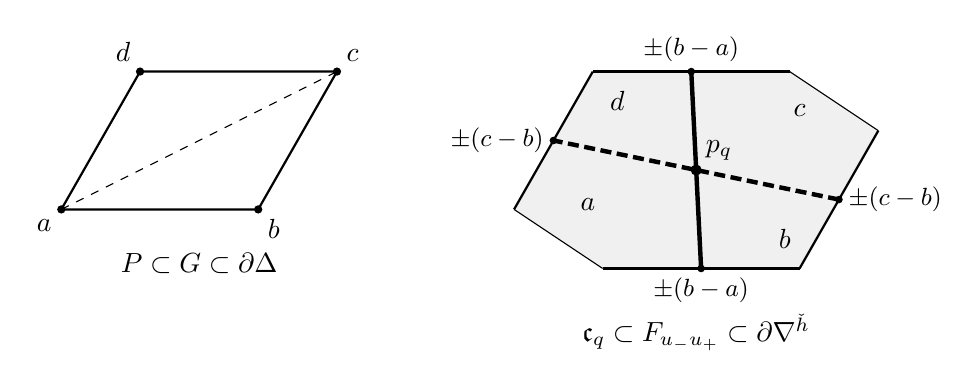
\begin{tikzpicture}[scale=1.25,>=stealth]
\coordinate (a) at (0,0); \coordinate (b) at (2,0); \coordinate (c) at (2.8,1.4); \coordinate (d) at (0.8,1.4);
\draw[thick] (a)--(b)--(c)--(d)--cycle;
\draw[dashed] (a)--(c);
\foreach \p/\l/\pos in {a/a/below left,b/b/below right,c/c/above right,d/d/above left}{\fill (\p) circle (1.2pt); \node[\pos] at (\p) {$\l$};}
\node at (1.4,-0.55) {$P\subset G\subset\partial\Delta$};
\begin{scope}[xshift=4.6cm]
\coordinate (A) at (0,0); \coordinate (As) at (0.9,-0.6); \coordinate (Bs) at (2.9,-0.6);
\coordinate (Cs) at (3.7,0.8); \coordinate (C) at (2.8,1.4); \coordinate (D) at (0.8,1.4);
\fill[gray!12] (A)--(As)--(Bs)--(Cs)--(C)--(D)--cycle;
\draw (A)--(As); \draw (Cs)--(C);
\draw[thick] (As)--(Bs); \draw[thick] (Bs)--(Cs); \draw[thick] (C)--(D); \draw[thick] (D)--(A);
\coordinate (p) at (1.85,0.4);
\coordinate (mab) at (1.9,-0.6); \coordinate (mbc) at (3.3,0.1); \coordinate (mcd) at (1.8,1.4); \coordinate (mda) at (0.4,0.7);
\draw[line width=1.6pt] (mab)--(p)--(mcd);
\draw[line width=1.6pt,dash pattern=on 4pt off 2pt] (mbc)--(p)--(mda);
\foreach \m in {mab,mbc,mcd,mda}{\fill (\m) circle (1.1pt);}
\fill (p) circle (1.6pt); \node[above right] at (p) {$p_q$};
\node at (0.75,0.05) {$a$}; \node at (2.75,-0.3) {$b$}; \node at (2.9,1.0) {$c$}; \node at (1.05,1.1) {$d$};
\node[below] at (mab) {\small $\pm(b-a)$}; \node[above] at (mcd) {\small $\pm(b-a)$};
\node[right] at (mbc) {\small $\pm(c-b)$}; \node[left] at (mda) {\small $\pm(c-b)$};
\node at (1.85,-1.25) {$\mathfrak c_q\subset F_{u_-u_+}\subset\partial\nabla^{\check h}$};
\end{scope}
\end{tikzpicture}
\caption{Left: a node parallelogram $P=abcd$ in a two-face $G$ of $\Delta$, with the diagonal $\{a,c\}$ dashed. Right: its carrying
cell $\mathfrak c_q=P+\operatorname{conv}\tau$ in the two-face $F_{u_-u_+}$ of $\nabla^{\check h}$, drawn for $\tau$ a segment; the
maximal cells $C_\pm$ lie on the two sides of the page. The thick edges have the two-point lower supports $\{a,b\}$, $\{b,c\}$,
$\{c,d\}$, $\{d,a\}$, and the four legs of $\Gamma$ join $p_q$ to their barycentres, labelled with their vanishing vectors. The four
complementary regions carry the charts of the lower rays $a,b,c,d$. The $b-a$ passage (solid) and the $c-b$ passage (dashed) are
the two pairs of opposite legs.}
\label{fig:node}
\end{figure}

\begin{lemma}[the node germ]\label{lem:nodegerm}
\begin{enumerate}
\item For $n\in P$ let $\pi_n$ be the chart $N_\R\to N_\R/\R n$, identified with $H_0=u_+^\perp$ by $x\mapsto x+\langle u_+,x\rangle n$.
Then for $n,n'\in P$,
\[
\pi_{n'}-\pi_n=\begin{cases}-\check h_+\,(n'-n)&\text{on }C_+,\\ -\bigl(\check h_++y_2(x)\bigr)(n'-n)&\text{on }C_-,\end{cases}\qquad
y_2(x):=\alpha(\mathfrak c)-\alpha(x),
\]
and $y_2\ge0$ on $C_+$, $y_2\le0$ on $C_-$, $y_2=0$ on $\mathfrak c$.
\item The affine structure off the discriminant near $\mathfrak c$ is unchanged if $\Gamma\cap\mathfrak c$ is replaced by any
four-legged star in $\mathfrak c$ whose legs end at the barycentres of the four edges of $\mathfrak c$ with a two-point lower
support, the region between consecutive legs receiving the chart of the lower ray of the boundary arc of $\mathfrak c$ that it
contains.
\item Let $b'$ be the centre of a translate $P+z\subset\mathfrak c$, $z$ a vertex of $\operatorname{conv}\tau$, and let
$\Gamma_{b'}$ be a star with vertex $b'$ whose legs leave $b'$ in the directions $\pm(b-a)$, $\pm(d-a)$ and continue inside
$\mathfrak c$ to the barycentres of the edges with lower supports $\{a,d\},\{b,c\},\{a,b\},\{c,d\}$, coinciding with the legs of
$\Gamma$ near these barycentres. Then a neighbourhood of $b'$ is integral affine isomorphic, with integral translations, to a
neighbourhood of the vertex of the discriminant in \cite[Ex.~6.1]{CBM}.
\end{enumerate}
\end{lemma}

\begin{proof}
(1) Since $\langle u_+,n\rangle=-1$, $N=(H_0\cap N)\oplus\Z n$, and $x\mapsto x+\langle u_+,x\rangle n$ is the lattice projection
along $n$ onto $H_0$. Hence $\pi_{n'}-\pi_n=\langle u_+,x\rangle(n'-n)$. On $C_+$, $\langle u_+,x\rangle=-\check h_+$. On $C_-$,
$\langle u_+,x\rangle=\alpha(x)+\langle u_-,x\rangle=\alpha(x)-\check h_-=-\check h_+-y_2(x)$. Since $\nabla^{\check h}$ is convex,
$\langle u_-,x\rangle\ge-\check h_-$ on $C_+$ and $\langle u_+,x\rangle\ge-\check h_+$ on $C_-$, which give the signs of $y_2$.

(2) By (1) the charts $\pi_n$, $n\in P$, differ by integral translations on $C_+$ and on $C_-$ separately, and by a map that is
not affine across $\mathfrak c$. So inside $\mathfrak c$ one needs only a closed set separating four regions, each containing the
vertices of $\mathfrak c$ with a given lower ray. Edges of $\mathfrak c$ with a one-point lower support join vertices with the same
lower ray, and the four edges with a two-point lower support separate the boundary of $\mathfrak c$ into four arcs with lower rays
$a,b,c,d$ in this cyclic order.

(3) Choose the origin at the lattice point $a+z$ and the basis $v_1=b-a$, $w_{u_-}$, $v_3=d-a$ of $H_0\cap N$, where $w_{u_-}$ is the
vector of Lemma~\ref{lem:primheight} for $(u,u')=(u_+,u_-)$: by that lemma $H_0\cap N=N_G\oplus\Z w_{u_-}$, and $v_1,v_3$ is a basis of
$N_G$ because $P$ is a unit parallelogram. Then $\alpha(v_1)=\alpha(v_3)=0$ and $\alpha(w_{u_-})=-1$, so the second coordinate of a point of $H_0$ is
$y_2$. In the coordinates $y=(y_1,y_2,y_3)$ of this basis, the chart of
the corner $a+iv_1+jv_3$ ($i,j\in\{0,1\}$) is, up to an integral translation, $y$ on $\{y_2\ge0\}$ and
$\bigl(I-(ie_1+je_3)e_2^{\mathsf T}\bigr)y$ on $\{y_2\le0\}$, by (1). Near $b'=(\tfrac12,0,\tfrac12)$ the region of the corner
$(i,j)$ is the quadrant $\{\operatorname{sign}(y_1-\tfrac12)=2i-1,\ \operatorname{sign}(y_3-\tfrac12)=2j-1\}$. This is the
atlas of \cite[Ex.~6.1]{CBM}: two triangular prisms glued along a unit square, with perpendicular prism directions $e_1,e_3$, the
monodromy-invariant plane $\langle e_1,e_3\rangle$, and the vertex at the barycentre of the square; the translations are
integral.
\end{proof}

The sign of the shear in (3), forced by the convexity of $\nabla^{\check h}$ through (1), is the one of \cite[Ex.~6.1]{CBM}, where it
is forced by the two prisms. With the barycentric placement, the vertex of $\Gamma$ sits at the barycentre of $\mathfrak c$, whose
position modulo the lattice is in general not that of $b'$; this is why the vertex is moved in (3).

\begin{lemma}[placement]\label{lem:placement}
Let $\Gamma'$ be $\Gamma$ with the star inside every carrying cell replaced by $\Gamma_{b'}$. There is a piecewise linear
homeomorphism $\phi_{\rm pl}$ of $B$ which preserves every closed face of $\nabla^{\check h}$ and every cell of $\mathscr P$, carries
$\Gamma'$ onto $\Gamma$ and the local system of $B\setminus\Gamma'$ to that of $B\setminus\Gamma$, and is supported in a compact
subset of the union of the open stars of the points $p_q$ in $\operatorname{Bar}\mathscr P$. It is isotopic to the identity
through homeomorphisms with the same support that preserve $\Gamma$ outside the carrying cells.
\end{lemma}

\begin{proof}
Both stars lie in the disc $\mathfrak c$, have the same four end points on $\partial\mathfrak c$, coincide near them, and have their
legs in the same cyclic order. So there is a piecewise linear homeomorphism of $\mathfrak c$, equal to the identity near
$\partial\mathfrak c$, carrying one to the other; by the Alexander trick \cite{Ale23}, \cite[Lemma~2.1]{FM12} it is isotopic to the
identity relative to a neighbourhood of $\partial\mathfrak c$. Extend it and the isotopy across the two sides of $\mathfrak c$ by a
product in a thin collar, tapering to the identity. The support is then a compact subset of the open star of $p_q$, which is an
open neighbourhood of $\operatorname{int}\mathfrak c$. By Lemma~\ref{lem:nodegerm}(2) both placements assign the charts to the four
complementary regions by the same rule, and $\phi_{\rm pl}$ preserves the regions, so it carries $\Lambda$ to $\Lambda$.
\end{proof}

The open stars of distinct points $p_q$ in $\operatorname{Bar}\mathscr P$ are disjoint, because no chain of cells contains two
different two-cells; so the modifications at different nodes do not interact. This holds even when the closed carrying cells of
two nodes meet, which happens: at an $A_1$ hexagon they may share a vertex with lower ray $o$, at a pentagon or an $A_2$ hexagon
they may share an edge with lower support $\{o,w\}$, and across an edge of $\Delta$ they may share an edge whose barycentre is a positive
vertex of $\Gamma$.

\begin{proof}[Proof of Proposition~\ref{prop:base}(2)]
The germ is described by Lemma~\ref{lem:nodegerm}(3), and the comparison of the two placements is
Lemma~\ref{lem:placement}.
\end{proof}

We work with the barycentric placement from now on; the node point is $p_q=b_{\mathfrak c_q}$. Relative tropical $2$-cycles
(Definition~\ref{def:relcycle}) are defined on triangulations in which $\Gamma$ is full, and $\operatorname{Bar}\mathscr P$ is
one by Lemma~\ref{lem:full}.


The stalks of $\iota_*\Lambda$ at the points of $\Gamma$ are computed in Lemma~\ref{lem:stalks}: on a leg in $F_{uu'}$, at a
negative vertex and at a node point of $F_{uu'}$ the stalk is $\{u,u'\}^\perp\cap N$, and at a positive vertex on the edge of
$\nabla^{\check h}$ dual to the triangle $\{u_1,u_2,u_3\}$ it is $\{u_1,u_2,u_3\}^\perp\cap N=\Z d$, with $d$ the common vanishing vector of
the three legs.

\emph{The discriminant in a two-face.} Let $G$ be a pentagon or a hexagon, $G^\circ=[u_-,u_+]$. Each node parallelogram $P$ of
$\sigma|_G$ has two legs whose lower supports are interior edges $[o,w]$ of $\sigma|_G$, which share the lower ray $o$ and are therefore
adjacent in the cyclic order at $p_q$, and two legs whose lower supports are edges of $\Delta$.

\begin{lemma}[arcs across interior edges]\label{lem:dualarc}
Let $\epsilon=[o,w]$ be an interior edge of $\sigma|_G$, and let $L$ and $L'$ be the two cells of $\sigma|_G$ containing it, with
two-cells $\mathfrak c_L$, $\mathfrak c_{L'}\subset F_{u_-u_+}$ as above. Then $\Gamma$ contains an arc from $b_{\mathfrak c_L}$ to
$b_{\mathfrak c_{L'}}$ that is a union of legs with lower support $\{o,w\}$, vanishing vector $\pm(w-o)$ and covector $\pm(u_+-u_-)$,
and whose interior points are edge points of $\Gamma$.
\end{lemma}

\begin{proof}
Let $\Gamma_\epsilon$ be the union of the legs with lower support $\{o,w\}$, a subgraph of $\Gamma$. The facet indices of the maximal cells
at such a leg take the value $-1$ at $o$, so they are $u_-$ and $u_+$, the only lattice points of $\Delta^\circ$ with this property ($o$ is
interior to $G$, and $G^\circ\cap M=\{u_-,u_+\}$). So every such leg lies in a two-cell $f\subset F_{u_-u_+}$ whose lower support contains
$\epsilon$: the segment $\epsilon$ itself, or a two-cell of $\Sigma'$ containing $\epsilon$ on which $u_\pm$ take the value $-1$, that is, $L$
or $L'$. We compute the number of legs of $\Gamma_\epsilon$ at each point.
\begin{itemize}
\item At $b_e$, $e$ an edge with lower support $\epsilon$: the facet indices around $e$ lie in $\{u_-,u_+\}$. If $e$ lies in one facet, so
that $j=1$ in Lemma~\ref{lem:edge}, no leg ends at $b_e$. If $b_e\in\Gamma_\epsilon$, then $j=2$, and by Lemma~\ref{lem:edge} exactly two legs
end at $b_e$, both with the lower support of $e$.
\item At $b_f$, $f$ a two-cell with lower support $\epsilon$ and $u_+(f)\ne u_-(f)$: $f$ has exactly two edges with lower support $\epsilon$
and no other edge with a two-point lower support, so two legs of $\Gamma_\epsilon$ end at $b_f$.
\item At $b_{\mathfrak c_L}$: the unique edge of $\mathfrak c_L$ with lower support $\epsilon$, the face selected by the outer normal of
$\epsilon$ in $L$, gives exactly one leg of $\Gamma_\epsilon$; likewise at $b_{\mathfrak c_{L'}}$. By the stack lemma no other two-cell over
$L$ or $L'$ carries a leg.
\end{itemize}
So $\Gamma_\epsilon$ is a finite graph in which $b_{\mathfrak c_L}$ and $b_{\mathfrak c_{L'}}$ have valency one and every other vertex has
valency two. The component of $b_{\mathfrak c_L}$ is therefore a path, whose other end has valency one and is not $b_{\mathfrak c_L}$; it is
$b_{\mathfrak c_{L'}}$. Its interior points are points $b_e$ in the interior of $F_{u_-u_+}$ and points $b_f$ with a two-point lower
support, which are edge points by Lemma~\ref{lem:types}. All its legs have the vanishing vector $\pm(w-o)$ and the covector $\pm(u_+-u_-)$.
\end{proof}

By Proposition~\ref{prop:L2}(2) this arc is the only arc of $\Gamma$ with lower support $\{o,w\}$. Applied to the interior edges
of Lemma~\ref{lem:subdiv}(3), the lemma gives the shape of $\Gamma$ in the two-face $F_{u_-u_+}$ of a del Pezzo face: at a pentagon, a cycle
through the two nodes and the negative vertex of the triangle, with one arc from node to node (across $[o,w_1]$ in the
coordinates~\eqref{eq:pentnormal}); at an $A_1$ hexagon, a cycle through the two nodes and the two negative vertices, with no arc from node
to node; at an $A_2$ hexagon, three arcs from node to node, across the edges $[o,w_j]$ with $j\equiv j_0\bmod2$, forming a cycle of
$\Gamma$ through the three nodes with no trivalent vertex. These configurations are used in Section~\ref{sec:cycles}; the lift of
Section~\ref{sec:lift} treats several nodes in one two-face in Section~\ref{ssec:lift-assembly}, and the resolution side in
Lemma~\ref{lem:resmove}.

\subsection{The mirror subdivision}\label{ssec:mirrorsub}
The mirror family of Section~\ref{ssec:mirrorfamily} uses a height $H=k_0\varphi+h_C$ on $\partial\Delta\cap N$, where $h_C$ induces a
refinement $\mathcal F_C$ of $\Sigma'$. The analysis near the node points (Section~\ref{ssec:member}) needs two properties of
$\mathcal F_C$: it agrees with $\Sigma'$ on the faces of dimension at most two, so that every node parallelogram is a cell, and the
three-cells of $\mathcal F_C$ containing a node parallelogram $P$ have all their lattice points off $P$ at lattice height one over the
plane of $P$. We construct $\mathcal F_C$ by pulling the lattice points of $\partial\Delta$ that are not vertices of $\Sigma'$, and show that
the second property then holds automatically. The subdivision $\Sigma'$ itself need not have it (Remark~\ref{rem:Sigmaheight}).

\emph{Fans and subdivisions of $\mathcal A$.} Let $\mathcal A=(\partial\Delta\cap N)\cup\{0\}$. We use the language of point configurations
\cite{DLRS}. A subdivision $\mathcal S$ of $\mathcal A$ is \emph{regular} if it is induced by a height $g\colon\mathcal A\to\R$: its cells are
the subsets $\mathfrak d=\{a\in\mathcal A:g(a)=\ell_{\mathfrak d}(a)\}$ for the affine functions $\ell_{\mathfrak d}\le g$ on $\mathcal A$ whose
equality set spans a face of the lower hull. Let $\hat g\colon\operatorname{conv}\mathcal A\to\R$ be the lower envelope, the largest convex
function with $\hat g\le g$ on $\mathcal A$; then $\hat g=\ell_{\mathfrak d}$ on $\operatorname{conv}\mathfrak d$, and
$\{\hat g=\ell_{\mathfrak d}\}=\operatorname{conv}\mathfrak d$. A complete fan in $N_\R$ that refines the fan over the faces of $\Delta$ and has
its rays generated by points of $\mathcal A$ is the fan of cones from $0$ over the cells of a subdivision of $\mathcal A$ all of whose maximal
cells contain $0$, the cells on $\partial\Delta$ being those of the fan; the fan carries a strictly convex piecewise linear function if and
only if the subdivision is regular, the function, normalised to vanish at $0$, being a height that induces the subdivision. By~\ref{hyp:P},
$\Sigma'$ is regular in this sense. A point $j\in\mathcal A$ is a \emph{vertex} of $\mathcal S$ if $\{j\}$ is a cell.

\begin{definition}[pulling]\label{def:pulling}
Let $\mathcal S$ be a subdivision of $\mathcal A$ and $j\in\mathcal A$. The \emph{pulling} $\operatorname{pull}_j\mathcal S$ keeps every cell
$\mathfrak d$ with $j\notin\operatorname{conv}\mathfrak d$, and replaces every cell $\mathfrak d$ with $j\in\operatorname{conv}\mathfrak d$ by the
cells $\{j\}\cup(\mathfrak d\cap F)$, for the faces $F$ of $\operatorname{conv}\mathfrak d$ with $j\notin F$ \cite[\S4.3]{DLRS}.
\end{definition}

The definition applies to every cell whose convex hull contains $j$, also when $j$ is not a point of the cell, as happens after an
earlier pulling has placed $j$ strictly above the lower hull.

\begin{lemma}[pulling preserves regularity]\label{lem:pullreg}
Let $g$ induce $\mathcal S$ and let $j\in\mathcal A$. Put $g_\eta(j)=\hat g(j)-\eta$ and $g_\eta=g$ on $\mathcal A\setminus\{j\}$. For $\eta>0$ small,
$g_\eta$ induces $\operatorname{pull}_j\mathcal S$. In particular $\operatorname{pull}_j\mathcal S$ is regular, $j$ is one of its vertices, and every
vertex of $\mathcal S$ other than $j$ remains a vertex. If $j\in\partial\Delta$ and every maximal cell of $\mathcal S$ contains $0$, then every
maximal cell of $\operatorname{pull}_j\mathcal S$ contains $0$.
\end{lemma}

\begin{proof}
Let $\mathfrak d$ be a cell with $j\in\operatorname{conv}\mathfrak d$, and $F$ a facet of $\operatorname{conv}\mathfrak d$ with $j\notin F$. Let
$\lambda_F$ be the affine function on $\operatorname{aff}\mathfrak d$, extended to the ambient space, with $\lambda_F=0$ on $F$ and $\lambda_F(j)=1$;
it is positive on $\operatorname{conv}\mathfrak d\setminus F$. The affine function $\ell_{\mathfrak d}-\eta\lambda_F$ agrees with $g_\eta$ at $j$,
because $\ell_{\mathfrak d}(j)=\hat g(j)$, and on $\mathfrak d\cap F$; it lies strictly below $g_\eta=g=\ell_{\mathfrak d}$ on
$\mathfrak d\setminus(F\cup\{j\})$. At a point $a\in\mathcal A\setminus(\mathfrak d\cup\{j\})$ we have $g(a)>\ell_{\mathfrak d}(a)$, and since $\mathcal A$ is
finite, $\ell_{\mathfrak d}(a)-\eta\lambda_F(a)<g(a)$ for $\eta$ small. So $\{j\}\cup(\mathfrak d\cap F)$ is a cell of the subdivision induced by
$g_\eta$, with convex hull $\operatorname{conv}(\{j\}\cup F)$; these convex hulls, over the facets $F$ not containing $j$, cover
$\operatorname{conv}\mathfrak d$. If $j\notin\operatorname{conv}\mathfrak d$, then $\hat g(j)>\ell_{\mathfrak d}(j)$, because
$\{\hat g=\ell_{\mathfrak d}\}=\operatorname{conv}\mathfrak d$; so for $\eta$ small $\ell_{\mathfrak d}(j)<g_\eta(j)$, and $\mathfrak d$ remains a
cell. Applying this to the maximal cells, the cells found cover $\operatorname{conv}\mathcal A$, so they are all the maximal cells of the
subdivision induced by $g_\eta$, which is therefore $\operatorname{pull}_j\mathcal S$. The point $j$ is a vertex of every cell
$\operatorname{conv}(\{j\}\cup F)$, and a vertex $v\ne j$ of $\mathcal S$ is kept because $j\notin\operatorname{conv}\{v\}$.

For the last statement, a maximal cell of $\mathcal S$ with $j$ in its convex hull is $\operatorname{conv}(\{0\}\cup C)$ with $C$ a cell on
$\partial\Delta$, and $j\in\operatorname{conv}C$ because $j\in\partial\Delta$ and $C$ lies in a supporting hyperplane of $\Delta$. The facets of
$\operatorname{conv}(\{0\}\cup C)$ are $C$ and the cones $\operatorname{conv}(\{0\}\cup F')$ over the facets $F'$ of $C$; those not containing
$j$ are of the second kind and contain $0$.
\end{proof}

Let $\mathcal F_C$ be the subdivision of $\partial\Delta$ obtained from $\Sigma'$ by pulling, one at a time and in any order, the lattice points
of $\partial\Delta$ that are not vertices of $\Sigma'$. By Lemma~\ref{lem:pullreg} it is induced by a height on $\mathcal A$, which we may take
rational; the function on $N_\R$ that is linear on the cone over each cell and equal to this height on its vertices is strictly convex on the
fan over $\mathcal F_C$. Multiplying it by a positive integer makes its linear functions integral. We let $h_C$ be such a function: strictly
convex on the fan over $\mathcal F_C$, inducing $\mathcal F_C$, with integral slopes and $h_C(0)=0$.

\begin{lemma}[the pyramid over a unit parallelogram]\label{lem:pyramid}
Let $P=abcd\subset G$ be a node parallelogram, $G^\circ=[u,u']$, and let $x\in u^\vee\cap N$ with $h_x:=e_{u'}(x)\ge1$. With $w_{u'}$ as in
Lemma~\ref{lem:primheight}, write
\[
x-a=\alpha(b-a)+\beta(d-a)+h_x\,w_{u'},\qquad\alpha,\beta\in\Z.
\]
Then $y:=a+\lceil\alpha/h_x\rceil(b-a)+\lceil\beta/h_x\rceil(d-a)+w_{u'}$ is the only lattice point of $\operatorname{conv}(P\cup\{x\})$ with
$e_{u'}=1$. If $h_x\ge2$, then $y$ is not a vertex of $\operatorname{conv}(P\cup\{x\})$.
\end{lemma}

\begin{proof}
By Lemma~\ref{lem:primheight}, $(b-a,d-a,w_{u'})$ is a basis of $u^\perp\cap N$, since $b-a,d-a$ is a basis of $N_G$ ($P$ is a unit parallelogram).
In the lattice coordinates $(s,t,e)$ of this basis with origin $a$ on $\operatorname{aff}(u^\vee)$, $e=e_{u'}$, $P=[0,1]^2\times\{0\}$ and
$x=(\alpha,\beta,h_x)$. The slice of $\operatorname{conv}(P\cup\{x\})$ at $e=1$ is $(1-1/h_x)P+x/h_x$, the product of the intervals
$[\alpha/h_x,\alpha/h_x+1-1/h_x]$ and $[\beta/h_x,\beta/h_x+1-1/h_x]$. Each has length $1-1/h_x$ and end points in $\frac1{h_x}\Z$; writing
$\alpha=mh_x+i$ with $0\le i<h_x$, the first interval is $[m+i/h_x,\,m+(i+h_x-1)/h_x]$, which contains exactly one integer, $\lceil\alpha/h_x\rceil$;
likewise for $\beta$. The vertices of $\operatorname{conv}(P\cup\{x\})$ lie at the levels $0$ and $h_x$, so for $h_x\ge2$ the point $y$ at level $1$ is
not a vertex.
\end{proof}

\begin{lemma}[a high apex forces a lattice point]\label{lem:hidden}
Let $\mathcal S$ be a subdivision of $\partial\Delta$ into lattice polytopes that induces $\sigma$ on the two-faces of $\Delta$. Let $P\subset G$ be a
node parallelogram, $G^\circ=[u,u']$, and $\omega$ the three-cell of $\mathcal S$ in $u^\vee$ containing $P$. If some vertex $x$ of $\omega$ has
$e_{u'}(x)\ge2$, then the point $y$ of Lemma~\ref{lem:pyramid} is a lattice point of $\omega$ that is not a vertex of $\omega$, and it lies in the
relative interior of the facet $u^\vee$.
\end{lemma}

\begin{proof}
$y\in\operatorname{conv}(P\cup\{x\})\subseteq\omega$. A vertex of $\omega$ lying in the subpolytope $\operatorname{conv}(P\cup\{x\})$ is a vertex of it,
and by Lemma~\ref{lem:pyramid} $y$ is not. Suppose $y$ lay in a face $G''$ of $\Delta$ of dimension at most two; we may take $G''\subseteq u^\vee$.
Then $\omega\cap G''$ is a face of $\omega$, hence a cell of $\mathcal S$ contained in $G''$, that is, a cell of $\sigma$ or a face of one. Such a cell
has no lattice points other than its vertices (Lemma~\ref{lem:subdiv}(4)), so $y$ would be a vertex of $\omega\cap G''$, hence of $\omega$, a
contradiction.
\end{proof}

\begin{proposition}\label{prop:pulling}
Let $\Delta$ be admissible and $\sigma$ a profile satisfying~\ref{hyp:P}, with any number of pentagons and of hexagons on either
branch. Then:
\begin{enumerate}
\item $\mathcal F_C$ is regular: there is a function $h_C$ with integral slopes, strictly convex on the fan over $\mathcal F_C$, that induces
$\mathcal F_C$; every maximal cell of the corresponding subdivision of $\mathcal A$ contains $0$;
\item $\mathcal F_C$ refines $\Sigma'$ and agrees with it on the faces of $\Delta$ of dimension at most two; so the two-cells of $\mathcal F_C$ in
two-faces of $\Delta$ are unimodular triangles and node parallelograms;
\item every lattice point of $\partial\Delta$ is a vertex of $\mathcal F_C$;
\item \emph{(height condition)} for every node parallelogram $P\subset G$, $G^\circ=[u,u']$, let $\omega_1\subseteq u^\vee$ and
$\omega_2\subseteq u'^\vee$ be the three-cells of $\mathcal F_C$ containing $P$. Every lattice point of $\omega_1$ not in $P$ has $e_{u'}=1$, and
every lattice point of $\omega_2$ not in $P$ has $e_u=1$.
\end{enumerate}
\end{proposition}

\begin{proof}
(1) By Lemma~\ref{lem:pullreg}, applied at each step, $\mathcal F_C$ is induced by a height on $\mathcal A$ and every maximal cell of
the corresponding subdivision of $\mathcal A$ contains $0$; the integral slopes of $h_C$ come from the choice of $h_C$ after the
definition of $\mathcal F_C$. (2) Pulling $j$ changes only the cells whose convex hull contains $j$, and refines
them. Every lattice point of a face of dimension at most two lies in $R$ and is a vertex of $\Sigma'$ (Section~\ref{ssec:faces}), so every
pulled point lies in the relative interior of a facet of $\Delta$, and no cell in a face of dimension at most two contains it. By induction
these cells are never changed. (3) Each pulled point becomes a vertex, and vertices are never lost (Lemma~\ref{lem:pullreg}).

(4) Let $\omega=\omega_1$. The set $\omega\cap u'^\vee=\omega\cap G$ is a face of $\omega$ and, by (2), a cell of $\sigma$ in $G$ containing $P$; so it is
$P$. Hence every vertex of $\omega$ off $P$ has $e_{u'}\ge1$. If a vertex had $e_{u'}\ge2$, Lemma~\ref{lem:hidden} would give a lattice point of
$\omega$ that is not a vertex of $\omega$; by (3) it is a vertex of $\mathcal F_C$, and a vertex of a polyhedral complex that lies in a cell is a
vertex of that cell. So every vertex of $\omega$ off $P$ has $e_{u'}=1$. As $e_{u'}$ is affine and takes values in $[0,1]$ on $\omega$, every lattice
point of $\omega$ has $e_{u'}\in\{0,1\}$, and those with $e_{u'}=0$ lie in $\omega\cap G=P$. The statement for $\omega_2$ follows by exchanging $u$
and $u'$.

The face type enters only through three facts, which hold for every profile: $\ell(G^\circ)=1$ at the face of $P$ (used in
Lemma~\ref{lem:primheight}); every cell of $\sigma$, and every face of one, has no lattice points besides its vertices (used in
Lemma~\ref{lem:hidden}; Lemma~\ref{lem:subdiv}(4) for pentagons and for hexagons on both branches); and every point of $R$, the hexagon centres
included, is a vertex of $\Sigma'$ (used in (2)). A node parallelogram is a two-cell of $\sigma|_G$, so no other cell of $\sigma|_G$ contains it; at an
$A_2$ hexagon this applies to each of the three rhombi, although they share edges pairwise.
\end{proof}

The lattice points of $\omega_1\cup\omega_2$ not in $P$ are the \emph{apexes} of $P$ in Section~\ref{ssec:member}. The proof of (4) shows more.

\begin{remark}\label{rem:Sigmaheight}
\begin{enumerate}
\item Let $\mathcal S$ be a regular subdivision of $\partial\Delta$ into lattice polytopes that induces $\sigma$ on the two-faces and in which the
three-cells containing node parallelograms have no lattice points other than their vertices. Then the height condition holds for $\mathcal S$, by
the argument of (4) with Lemma~\ref{lem:hidden}. In particular it holds for $\Sigma'$ itself whenever every lattice point of $\partial\Delta$ is a
vertex of $\Sigma'$; this is the case for the subdivisions $\Sigma'$ of the examples $X_9$, $X_{19}$ and $X_{20}$ in Section~\ref{sec:examples}, and there
$\mathcal F_C=\Sigma'$.
\item In general a subdivision $\Sigma'$ satisfying~\ref{hyp:P} does not satisfy the height condition. The polytope $\Delta_9$ of the example
$X_9$ has a subdivision satisfying~\ref{hyp:P} whose vertices are all the lattice points of $\partial\Delta_9$ except $(-1,0,0,0)$; in it the three-cell over one of the pentagon parallelograms $P$, in the facet $u=(1,-1,-1,-1)$ with
$u'=(0,1,-1,-1)$, is the pyramid $\operatorname{conv}(P\cup\{(0,1,0,0)\})$ with $e_{u'}((0,1,0,0))=2$, whose only lattice point at height one is $(-1,0,0,0)$.
Pulling this point gives the $\Sigma'$ of Section~\ref{sec:examples}. On the list of Section~\ref{ssec:list}, the subdivisions $\Sigma'$ that
the linear program of~\ref{hyp:P} returns violate the height condition on $7$ of the $364$ hexagon-free polytopes satisfying~\ref{hyp:P}, with apexes
at height $2$ or $3$, while $\mathcal F_C$ satisfies it on all of them (exact computation).
\end{enumerate}
\end{remark}

\subsection{When (Proj) fails}\label{ssec:proj}
This section does not assume~\ref{hyp:P}. We show that~\ref{hyp:P} is equivalent to the projectivity of $X'_\sigma\to X$, and describe what a failure
means for the exceptional surfaces. For an interior edge $\epsilon=[o,w_j]$ of $\sigma|_G$, $G$ a pentagon or a hexagon, put
\[
I_\epsilon:=e_{w_{j-1}}+e_{w_{j+1}}-a_je_{w_j}+(a_j-2)e_o\in\Z^R,\qquad (w_{j-1}-o)+(w_{j+1}-o)=a_j(w_j-o).
\]
For a function $\psi$ on $G\cap N$ that is affine on the cells $L\supset T_{j-1}$ and $L'\supset T_j$ of $\sigma|_G$ at $\epsilon$,
$\langle I_\epsilon,\psi\rangle=\psi(w_{j+1})-\ell_L(w_{j+1})$, where $\ell_L$ is the affine function equal to $\psi$ on $L$: the \emph{bend} of $\psi$
across $\epsilon$, measured at a point at lattice distance one from $\epsilon$.

\begin{lemma}\label{lem:projLP}
\ref{hyp:P} holds if and only if there is $\psi\in\Q^R$ with $\langle\circv_q,\psi\rangle=0$ for every $q\in Q$ and $\langle I_\epsilon,\psi\rangle>0$ for every
interior edge $\epsilon$ of $\sigma$ at a pentagon or a hexagon.
\end{lemma}

\begin{proof}
A function $\psi$ on $G\cap N$ induces $\sigma|_G$ if and only if it is affine on each cell, which for a parallelogram is $\langle\circv_q,\psi\rangle=0$,
and bends positively across each interior edge; local convexity across the interior edges implies convexity on $G$. If~\ref{hyp:P} holds, the
restriction to $R$ of a strictly convex function inducing $\Sigma'$ has these properties. Conversely, given $\psi$, let $\mathcal S_\Phi$ be the
regular subdivision of $\Phi\cap R$ induced by $\psi$ on each facet $\Phi$ of $\Delta$. On a face of $\Phi$ it restricts to the regular subdivision
induced by the restriction of $\psi$, which on two-faces is $\sigma$ and on edges is trivial; so the $\mathcal S_\Phi$ agree on common faces and form a
subdivision $\mathcal S$ of $\partial\Delta$ with vertices in $R$. Let $g$ be the function on $N_\R$ that is linear on the cone over each cell of
$\mathcal S$ and equals $\psi$ on $R$. It is convex across the walls inside the cones over facets. The function $\varphi$ that equals $1$ on
$\partial\Delta$ and is linear on the cones over the facets is convex, with positive bend across each wall between two facet cones, and linear
inside them; so for $\gamma$ large, $g+\gamma\varphi$ is strictly convex on the fan over $\mathcal S$. The toric variety of this fan is projective, its rays pass
through points of $R\subset\partial\Delta$, and it induces $\sigma$.
\end{proof}

Let $\widehat X$ be the small resolution with the chosen diagonals, which exists as a compact complex manifold without~\ref{hyp:P}
(Section~\ref{ssec:partialres}). For an interior edge $\epsilon=[o,w_j]$ of $\sigma|_G$, let $f_\epsilon\subset E'_G$ be the torus-invariant curve of
the cone over $\epsilon$ in the local model $U'_{G,\sigma}$, and $\tilde f_\epsilon\subset E_G$ its proper transform in $\widehat X$, which is the
curve $f_j$ of Proposition~\ref{prop:classical}. In the local model of $\widehat X$ the curve $\tilde f_\epsilon$ is the curve of the wall
$\operatorname{cone}(o,w_j)$ between the cones over $T_{j-1}$ and $T_j$, and the wall relation
$w_{j-1}+w_{j+1}-a_jw_j+(a_j-2)o=0$ gives $(D_r\cdot\tilde f_\epsilon)_{r\in R}=I_\epsilon$.

\begin{proposition}\label{prop:projective}
The following are equivalent:
\begin{enumerate}
\item \ref{hyp:P} holds;
\item $X'_\sigma\to X$ is projective;
\item there are no rational numbers $y_\epsilon\ge0$, not all zero, and $\nu_q$ with
$\sum_\epsilon y_\epsilon[\tilde f_\epsilon]=\sum_q\nu_q[C_q]$ in $H_2(\widehat X;\Q)$.
\end{enumerate}
\end{proposition}

\begin{proof}
(1)$\Rightarrow$(2): $X'_\sigma\to X$ is induced by the projective morphism $P'_\sigma\to\mathbb P_\Delta$. (2)$\Rightarrow$(3): let $L$ be relatively
ample for $X'_\sigma\to X$ and $\pi\colon\widehat X\to X'_\sigma$. Then $\pi^*L\cdot C_q=0$, since $C_q$ is contracted by $\pi$, and
$\pi^*L\cdot\tilde f_\epsilon=L\cdot f_\epsilon>0$, since $f_\epsilon$ is a curve in a fibre of $X'_\sigma\to X$. A relation as in (3) would pair with
$\pi^*L$ to a positive number on the left and to $0$ on the right. (3)$\Rightarrow$(1): if~\ref{hyp:P} fails, the linear system of
Lemma~\ref{lem:projLP} is infeasible, and by the Farkas--Motzkin alternative there are $y_\epsilon\ge0$, not all zero, and $\nu_q$ with
$\sum_\epsilon y_\epsilon I_\epsilon=\sum_q\nu_q\circv_q$ in $\Q^R$. By Proposition~\ref{prop:partialres}(2) and the computation above, the class
$\sum_\epsilon y_\epsilon[\tilde f_\epsilon]-\sum_q\nu_q[C_q]$ has zero image under~\eqref{eq:injection}, which is injective without~\ref{hyp:P}
(Lemma~\ref{lem:H2}); so it vanishes.
\end{proof}

A relation as in (3) is a \emph{Farkas certificate}. Where~\ref{hyp:P} fails there is no toric variety $P'_\sigma$, no subdivision
$\Sigma'$ and no base $B'_\sigma$, and the methods of this paper do not apply.

\section{The dual-pair complex}\label{sec:dualpair}

The base $B'_\sigma$ of $X'_\sigma$ and the base $B_Y$ of the mirror family are built from the same two subdivisions,
of $\partial\Delta^\circ$ by $\mathcal T$ and of $\partial\Delta$ by a fan-side subdivision, with the roles of Newton side and fan side
exchanged. Gross proved that the base built from $\Sigma'$ is Legendre dual, after a rescaling of the polarization, to a
base on $\partial\nabla^{m_0h+m_1\varphi}$, for a suitable $h$ inducing $\Sigma'$ and suitable positive integers $m_0,m_1$, built from the
same $\Sigma'$ with a decomposition that he constructs from the polarization \cite[Thms.~3.21, 3.25, 3.26]{Gross2005}
(Remark~\ref{rem:DLT}); the discrete Legendre transform matches the cells of two polyhedral decompositions. The
decompositions attached to the degenerations used here need not be Legendre dual to one another (compare
\cite[\S3, after Rem.~3.18]{Gross2005}), and the mirror base is built from the pulling refinement $\mathcal F_C$ of
$\Sigma'$ rather than from $\Sigma'$ itself. This section therefore introduces a coarser structure, used in both parts of
the paper: a regular cell decomposition of each base whose cells are indexed by pairs of dual cells of $\mathcal T$ and of
the subdivision of $\partial\Delta$ (Proposition~\ref{prop:L1}). Its face poset is the same on both bases, it needs no
polarization, and it carries the discriminants (Proposition~\ref{prop:L2}) and a flat perfect pairing between the two
local systems of integral tangent vectors (Proposition~\ref{prop:L3}). Section~\ref{sec:cycles} uses it to compute with
relative tropical $2$-cycles on $B'_\sigma$, and Section~\ref{sec:legendre} to transfer them to $B_Y$. The proof that the
cells are balls is in Appendix~\ref{app:legendre}.

\subsection{Faces, decompositions and charts}\label{ssec:leg-setting}
Throughout this section $\mathcal T$ and $\check h$ are as in Section~\ref{ssec:tropical}, with the normalisation of
Section~\ref{ssec:gross}: $\mathcal T$ is a unimodular triangulation of $\partial\Delta^\circ$ refining its faces, and the
integral height $\check h$ and $\check h':=\check h-\check\varphi$ are strictly convex on the fan over $\mathcal T$, that is,
convex, with the cones over the tetrahedra of $\mathcal T$ as their maximal domains of linearity. In the language of
Section~\ref{ssec:conventions}, $(\Delta^\circ,\mathcal T,\check h)$ is the Newton side of the degeneration of $X'_\sigma$.

\begin{definition}[fan-side subdivisions]\label{def:fanside}
A \emph{fan-side subdivision} is a subdivision $\mathcal F$ of $\partial\Delta$ into lattice polytopes, refining the faces of
$\Delta$, that is induced by a function $h\colon N_\R\to\R$ which is piecewise linear and strictly convex on the fan over
$\mathcal F$: convex, with the cones over the cells of $\mathcal F$ as its maximal domains of linearity.
\end{definition}

A fan-side subdivision is a regular polyhedral subdivision of $\partial\Delta$ in the sense of \cite[\S2.3]{DLRS}, and the fan over it
is the fan of a projective toric variety refining $\mathbb P_\Delta$. The fan-side subdivisions of this paper are $\Sigma'$
(Hypothesis~\ref{hyp:P}), the pulling refinement $\mathcal F_C$ (Section~\ref{ssec:mirrorsub}) and the regular
refinements of Section~\ref{sec:resolution}.

Cells of $\mathcal T$ are denoted $\tau$, cells of $\mathcal F$ are denoted $\omega$, vertices of $\mathcal T$ are denoted
$u,u'$ and vertices of $\mathcal F$ are denoted $n,n'$. For $\tau\in\mathcal T$ and $\omega\in\mathcal F$ put
\begin{gather*}
\tau^\vee=\{n\in\Delta:\langle u,n\rangle=-1\text{ for all vertices $u$ of $\tau$}\},\\
\omega^\vee=\{m\in\Delta^\circ:\langle m,n\rangle=-1\text{ for all vertices $n$ of $\omega$}\}.
\end{gather*}
If $G$ is the smallest face of $\Delta^\circ$ containing $\tau$, then $\tau$ meets the relative interior of $G$, and an
affine function that is $\ge-1$ on $G$ and equal to $-1$ at a relative interior point is $-1$ on $G$; so $\tau^\vee$ is
the face of $\Delta$ dual to $G$, of dimension $3-\dim G\le3-\dim\tau$. The same holds for $\omega^\vee$. We write
$\lgri Z$ for the relative interior of a convex set $Z$, $\operatorname{cone}(\tau)=\R_{\ge0}\tau$, and $L_\tau\subset M_\R$
for the linear span of $\tau$; since the vertices of $\tau$ lie in a hyperplane $\{\langle\,\cdot\,,n\rangle=-1\}$,
$\dim L_\tau=\dim\tau+1$.

\begin{lemma}[faces]\label{lem:faces}
For $\tau\in\mathcal T$ let $\nabla^{\check h'}_\tau=\{w\in\nabla^{\check h'}:\langle u,w\rangle=-\check h'(u)\text{ for all
vertices }u\text{ of }\tau\}$, where $\nabla^{\check h'}=\{w\in N_\R:\langle m,w\rangle\ge-\check h'(m)\text{ for all }m\in
M_\R\}$.
\begin{enumerate}
\item $\nabla^{\check h'}_\tau$ is the face of the polytope $\nabla^{\check h'}$ with inner normal cone
$\operatorname{cone}(\tau)$; $\dim\nabla^{\check h'}_\tau=3-\dim\tau$, and $\nabla^{\check h'}_\tau\subseteq\nabla^{\check
h'}_{\tau'}$ if and only if $\tau\supseteq\tau'$.
\item $\nabla^{\check h}=\Delta+\nabla^{\check h'}$, its normal fan is the fan over $\mathcal T$, and the face with inner
normal cone $\operatorname{cone}(\tau)$ is $F_\tau=\tau^\vee+\nabla^{\check h'}_\tau$. In particular $\tau^\vee\ne\emptyset$,
$\dim F_\tau=3-\dim\tau$, and $F_\tau\subseteq F_{\tau'}$ if and only if $\tau\supseteq\tau'$.
\end{enumerate}
\end{lemma}
We write $F_u=F_{\{u\}}$ for the facets and $F_{uu'}=F_{[u,u']}$ for the two-faces. The proof is in
Appendix~\ref{app:leg-faces}.

\emph{Gross's decomposition.} Let $\widetilde\Sigma$ be the normal fan of the epigraph $\mathrm{Epi}=\{(m,l):m\in\Delta^\circ,\
l\ge\check h'(m)\}$ \cite[Prop.~3.7]{Gross2005}, and for a vertex $u$ of $\mathcal T$ let $\widetilde\Sigma_u$ be its normal
cone at the vertex $(u,\check h'(u))$. The \emph{Cayley polytope} of $u$ is
\[
\mathrm{Cay}_u=\operatorname{conv}\bigl(u^\vee\times\{0\}\cup\nabla^{\check h'}_u\times\{1\}\bigr)\subset N_\R\oplus\R .
\]
It lies in the affine hyperplane $\{\langle u,y\rangle+(\check h(u)-2)l=-1\}$, since $\langle u,a\rangle=-1$ for $a\in u^\vee$
and $\langle u,w\rangle=-\check h'(u)=1-\check h(u)$ for $w\in\nabla^{\check h'}_u$. The maximal cones of $\widetilde\Sigma$ are
the $\widetilde\Sigma_u$ and the normal cone $\widetilde\Sigma_{\rm up}=\operatorname{cone}(\nabla^{\check h'}\times\{1\})$ at
the vertex $(0,0)$ of $\mathrm{Epi}$ \cite[Prop.~3.7]{Gross2005}.

Given a fan-side subdivision $\mathcal F$ with function $h$, we fix the following subdivision $\widetilde\Sigma'$ of $\widetilde\Sigma$:
on each $\widetilde\Sigma_u$ its cones are the cones over the cells of the regular subdivision of the point configuration
$(u^\vee\cap N)\times\{0\}\cup\operatorname{vert}\nabla^{\check h'}_u\times\{1\}$ with the heights $h(a)$ at $(a,0)$ and $0$
at $(w,1)$, and $\widetilde\Sigma_{\rm up}$ is not subdivided. These subdivisions agree on common faces, since the heights
are global and vanish on the upper points. The trace of $\widetilde\Sigma'$ on $N_\R\times\{0\}$ is the fan over
$\mathcal F$, and its other rays are generated by the vectors $(w,1)$, $w$ a vertex of $\nabla^{\check h'}$. Such a $w$ is a
lattice point: it is $\nabla^{\check h'}_\tau$ for a tetrahedron $\tau=\{u_1,\dots,u_4\}$ of $\mathcal T$, so $\langle
u_i,w\rangle=-\check h'(u_i)\in\Z$, and $u_1,\dots,u_4$ is a basis of $M$ because $\mathcal T$ is unimodular. So $(w,1)$
is primitive, and $\widetilde\Sigma'$ is good for $\mathcal F$ in the sense of \cite[Def.~3.8]{Gross2005}. It is the
subdivision of \cite[Rem.~3.18]{Gross2005} determined by the values $h$ on $N_\R\times\{0\}$ and $0$ on
$\widetilde\Sigma_{\rm up}$, because on $\widetilde\Sigma_u$ the lower envelope of these values is the cone over the lower
envelope of the heights on the slice $\mathrm{Cay}_u$ (Lemma~\ref{lem:cayley}(1)). We let $B_X=B_X(\mathcal F)$ be
$\partial\nabla^{\check h}$ with the decomposition $\mathscr P_X=\mathscr P^{\widetilde\Sigma'}_\nabla$ of
\cite[Def.~3.13]{Gross2005}: a mixed cone with lower generators $\omega\times\{0\}$ and upper generators
$\tau_1\times\{1\}$ gives the cell $\omega+\operatorname{conv}\tau_1$. For $\mathcal F=\Sigma'$ this is the base
$B'_\sigma$ with its decomposition $\mathscr P$ (Section~\ref{ssec:gross}).

\begin{lemma}[the cells as a mixed subdivision]\label{lem:cayley}
\begin{enumerate}
\item $\widetilde\Sigma_u$ is the cone over $\mathrm{Cay}_u$.
\item For $\tau\in\mathcal T$, the cells of $\mathscr P_X$ contained in $F_\tau$ are the cells of the regular mixed
subdivision of $\tau^\vee+\nabla^{\check h'}_\tau$ with the heights $h$ on $\tau^\vee\cap N$ and $0$ on
$\nabla^{\check h'}_\tau$: the projections to $N_\R$ of the bounded faces of $\widehat A_\tau+\widehat\nabla_\tau$, where
\[
\widehat A_\tau=\operatorname{conv}\{(a,h(a)):a\in\tau^\vee\cap N\}+\R_{\ge0}(0,1),\qquad
\widehat\nabla_\tau=\nabla^{\check h'}_\tau\times\{0\}+\R_{\ge0}(0,1).
\]
Each such cell is $c=\omega+\nabla^{\check h'}_{\tau'}$ with $\omega\in\mathcal F$, $\omega\subseteq\tau^\vee$, and
$\tau'\in\mathcal T$, $\tau'\supseteq\tau$, and $\omega$ and $\tau'$ are determined by $c$.
\end{enumerate}
\end{lemma}
The proof, by the Cayley trick, is in Appendix~\ref{app:leg-faces}. For a cell $c$ of $\mathscr P_X$ we call $\omega(c)$
its \emph{lower support}, as in Section~\ref{ssec:tropical}, and the $\tau(c)\in\mathcal T$ with $\lgri
c\subseteq\lgri F_{\tau(c)}$ its \emph{face label}; $F_{\tau(c)}$ is the smallest face of $\nabla^{\check h}$ containing
$c$. If $c\subseteq c'$, then $\tau(c)\supseteq\tau(c')$ and $\omega(c)\subseteq\omega(c')$, the latter because the lifted
face of $c$ is a face of the lifted face of $c'$. The barycentric subdivision $\lgBar\mathscr P_X$ has one simplex for
each chain $c_0\subsetneq\dots\subsetneq c_k$ of cells.

\emph{Regions, discriminant and charts.} For a vertex $n$ of $\mathcal F$ let $\widetilde R_n$ be the union of the open
simplices of $\lgBar\mathscr P_X$ whose chain has $\omega(c_0)=\{n\}$, and let $\Gamma_X$ be the union of the closed
simplices whose chain has $\dim\omega(c_0)\ge1$ and $\dim\tau(c_k)\ge1$. A maximal such chain is $e\subsetneq f$ with $f$
a two-cell in a two-face $F_{uu'}$ and $e$ an edge of $f$ with a two-point lower support; we call the segment
$[b_e,b_f]$ between their barycentres a \emph{leg} of $\Gamma_X$. For $\mathcal F=\Sigma'$ these are the legs of
Section~\ref{ssec:tropical} (Lemma~\ref{lem:monodromy}), and $\Gamma_X$ is the discriminant $\Gamma$ of $B'_\sigma$.

\begin{lemma}[charts]\label{lem:charts}
\begin{enumerate}
\item $\widetilde R_n$ is open. If $b\in\widetilde R_n$, then $\langle u,n\rangle=-1$ for every facet $F_u$ containing
$b$, and the projection $\pi_n\colon N_\R\to N_\R/\R n$ restricts to a homeomorphism of a neighbourhood of $b$ in $B_X$
onto an open set, which on each facet $F_u$ is the restriction of an affine isomorphism $\operatorname{aff}F_u\to
N_\R/\R n$ with linear part the lattice isomorphism $u^\perp\cap N\to N/\Z n$.
\item $B_X\setminus\Gamma_X=\bigcup_u\operatorname{int}F_u\cup\bigcup_n\widetilde R_n$, and $\Gamma_X$ is the union of the
open simplices whose chain has $\dim\omega(c_0)\ge1$ and $\dim\tau(c_k)\ge1$.
\item The facet charts on the $\operatorname{int}F_u$ and the projections $\pi_n$ on the $\widetilde R_n$ form an integral
affine atlas on $B_X\setminus\Gamma_X$, which restricts to Gross's structure \cite[Prop.~3.14]{Gross2005} on the
complement of Gross's discriminant.
\end{enumerate}
\end{lemma}
We write $\Lambda_X$ for the local system of integral tangent vectors of this structure. For $\mathcal F=\Sigma'$ it is
the local system $\Lambda$ of Section~\ref{ssec:tropical}. The proof is in Appendix~\ref{app:leg-faces}.

\emph{The mirror base.} Let $H\colon N_\R\to\R$ be piecewise linear on the fan over $\mathcal F$, with integral slopes (on
each cone of that fan $H$ is the restriction of an element of $M$), and such that $H':=H-\varphi$ is strictly convex on
that fan. The height $H=k_0\varphi+h_C$ of the mirror family (Section~\ref{ssec:mirrorfamily}) is such a function for
$\mathcal F=\mathcal F_C$: $\varphi$ is convex and linear on the cones over the cells of $\mathcal F_C$, so
$H'=(k_0-1)\varphi+h_C$, $k_0\ge1$, has the maximal domains of linearity of $h_C$; and $H$ has integral slopes because
$\varphi$ does, $\Delta$ being reflexive, and $h_C$ does by choice. The vertices of $\nabla^{H'}$ are lattice points: the
vertex with inner normal cone $\operatorname{cone}(\omega)$, $\omega$ a maximal cell, is $-m_\omega$, where $m_\omega\in M$
is the slope of $H'$ on $\operatorname{cone}(\omega)$. The \emph{mirror base} is $B_Y=\partial\nabla^H$,
$\nabla^H=\{m\in M_\R:\langle m,n\rangle\ge-H(n)\ \forall n\}$. It is the same construction with the roles of
$(\Delta^\circ,\mathcal T,\check h)$ and $(\Delta,\mathcal F,H)$ exchanged: $(\Delta,\mathcal F,H)$ is the Newton side and
$(\Delta^\circ,\mathcal T,\check h)$ the fan side. Its faces are $F^*_\omega=\omega^\vee+\nabla^{H'}_\omega$,
$\omega\in\mathcal F$, with $\nabla^{H'}_\omega$ the face of $\nabla^{H'}$ with inner normal cone
$\operatorname{cone}(\omega)$; its decomposition $\mathscr P_Y$ is defined by the heights $\check h$ on the lower points and
$0$ on the upper vertices; a cell $c$ of $\mathscr P_Y$ has a face label $\omega_Y(c)\in\mathcal F$ and a lower support
$\tau_Y(c)\in\mathcal T$; the regions are the $\widetilde R^*_u$, with charts $M_\R\to M_\R/\R u$; the facet $F^*_n$ carries
the lattice $n^\perp\cap M$; and the discriminant $\Gamma_Y$ and the local system $\Lambda_Y$ are defined as above.
Lemmas~\ref{lem:faces}--\ref{lem:charts} hold for $B_Y$ with the same proofs, which use only the strict convexity of the
Newton-side function ($\check h'$, respectively $H'$) and of the fan-side function ($h$, respectively $\check h$). The
subdivision of $\widetilde\Sigma_Y$ that defines $\mathscr P_Y$ is good in the sense of \cite[Def.~3.8]{Gross2005}, by the
argument above with the vertices of $\nabla^{H'}$ in place of those of $\nabla^{\check h'}$. So, by
\cite[Prop.~3.14]{Gross2005} with the roles exchanged, $(B_Y,\mathscr P_Y)$ is the dual intersection complex of Gross's toric
degeneration $X'_Y\subset X(\widetilde\Sigma'_Y)$ \cite[Thm.~3.10]{Gross2005} attached to the good subdivision
$\widetilde\Sigma'_Y$ that defines $\mathscr P_Y$. Its equation is $ts+s^0=0$, with $s^0$ the section given by the lattice
point $(0,0)$ and $s$ a general section with Newton polytope $\{(n,l):n\in\Delta,\ l\ge H'(n)\}$; the members
$\{\sum_nc_nt^{H(n)}x^n=0\}$ of the mirror family with $c_0=1$ have this form, with $s=\sum_{n\ne0}c_nt^{H'(n)}x^n$, since
$H=H'+\varphi$, $\varphi=1$ on $\partial\Delta$ and $H(0)=0$. Since $H(0)=0$, the
polytope $\nabla^H$ is the region on which the term $n=0$ of the tropical polynomial $m\mapsto\min_n(H(n)+\langle
m,n\rangle)$ attains the minimum, and $B_Y$ is the target of Yamamoto's tropical contraction of the tropical
hypersurface \cite[Thm.~1.2(2), (5.36), Prop.~5.4]{Ya21}; we do not use the contraction. We write $B_X(\mathcal F)$ and
$B_Y(\mathcal F)$ when the fan-side subdivision must be specified. Thus $B'_\sigma=B_X(\Sigma')$, and the mirror base of this paper is
$B_Y=B_Y(\mathcal F_C)$ with the height $H$ of Section~\ref{ssec:mirrorfamily}.

\subsection{The dual-pair complex}\label{ssec:leg-mixed}
\begin{definition}[dual pairs]\label{def:DP}
A \emph{dual pair} is a pair $(\tau,\omega)\in\mathcal T\times\mathcal F$ with $\langle u,n\rangle=-1$ for all vertices $u$
of $\tau$ and $n$ of $\omega$; equivalently $\omega\subseteq\tau^\vee$, or $\tau\subseteq\omega^\vee$. The set $\lgDP$ of
dual pairs is ordered by $(\tau,\omega)\preceq(\tau',\omega')$ if $\tau\supseteq\tau'$ and $\omega\supseteq\omega'$. We
put $\dim{\mathfrak p}=3-\dim\tau-\dim\omega$ for ${\mathfrak p}=(\tau,\omega)$; since $\dim\omega\le\dim\tau^\vee\le3-\dim\tau$, $\dim{\mathfrak p}\ge0$.
\end{definition}
In the language of Batyrev duality, $(\tau,\omega)$ is a dual pair if and only if $\tau$ and $\omega$ lie in a pair of
mutually dual faces of $\Delta^\circ$ and $\Delta$.

\begin{definition}[labels]\label{def:strata}
A point $b\in B_X$ lies in the open simplex of a unique chain $c_0\subsetneq\dots\subsetneq c_k$ of $\mathscr P_X$; put
$\operatorname{lab}_X(b)=(\tau(c_k),\omega(c_0))$, the face label of the top and the lower support of the bottom. For $b\in B_Y$ in
the open simplex of a chain $c_0\subsetneq\dots\subsetneq c_k$ of $\mathscr P_Y$, put
$\operatorname{lab}_Y(b)=(\tau_Y(c_0),\omega_Y(c_k))$. For ${\mathfrak p}\in\lgDP$ let $C_X({\mathfrak p})=\operatorname{lab}_X^{-1}({\mathfrak p})$ and $C_Y({\mathfrak p})=\operatorname{lab}_Y^{-1}({\mathfrak p})$.
\end{definition}

\begin{proposition}[the dual-pair complex]\label{prop:L1}
\begin{enumerate}
\item $\operatorname{lab}_X$ and $\operatorname{lab}_Y$ take values in $\lgDP$.
\item The sets $C_X({\mathfrak p})$, ${\mathfrak p}\in\lgDP$, are the open cells of a regular CW decomposition of $B_X$ with face poset
$(\lgDP,\preceq)$: each closure $\overline{C_X({\mathfrak p})}=\bigcup_{{\mathfrak q}\preceq {\mathfrak p}}C_X({\mathfrak q})$ is a subcomplex of $\lgBar\mathscr P_X$ and a
piecewise linear ball of dimension $\dim{\mathfrak p}$, with boundary sphere $\bigcup_{{\mathfrak q}\prec {\mathfrak p}}C_X({\mathfrak q})$. In particular every $C_X({\mathfrak p})$ is
nonempty.
\item The same holds for the $C_Y({\mathfrak p})$ on $B_Y$, with the same poset.
\item There is a piecewise linear homeomorphism $\mathcal L\colon B_X\to B_Y$ with $\mathcal L(C_X({\mathfrak p}))=C_Y({\mathfrak p})$ for all
${\mathfrak p}\in\lgDP$, and any two such homeomorphisms are isotopic through homeomorphisms with this property.
\item $C_X(\tau,\omega)\subseteq\lgri F_\tau$ and $C_Y(\tau,\omega)\subseteq\lgri F^*_\omega$. Moreover, for every
$\tau\in\mathcal T$ and every vertex $n$ of $\mathcal F$, $\lgri F_\tau=\bigcup_\omega C_X(\tau,\omega)$ and $\widetilde
R_n\cap\lgri F_\tau=C_X(\tau,n)$; in particular $\operatorname{int}F_u=\bigcup_\omega C_X(u,\omega)$ and $\widetilde
R_n=\bigcup_\tau C_X(\tau,n)$. Likewise on $B_Y$, with the roles of $\tau$ and $\omega$ exchanged. Hence
$\mathcal L(\operatorname{int}F_u)=\widetilde R^*_u$ and $\mathcal L(\widetilde R_n)=\operatorname{int}F^*_n$:
$\mathcal L$ exchanges the open facets with the regions.
\end{enumerate}
\end{proposition}
We call the decomposition of (2) and (3) the \emph{dual-pair complex} of $B_X$ and of $B_Y$, and a homeomorphism as in
(4) a \emph{dual-pair homeomorphism}. On a face $F_\tau$ the cells $C_X(\tau,\omega)$ correspond to the cells of the polyhedral
complex dual to the regular subdivision $\mathcal F|_{\tau^\vee}$, that is, of the tropical hypersurface of
$m\mapsto\min_{a\in\tau^\vee\cap N}(h(a)+\langle m,a\rangle)$ \cite[\S3.1]{MS}, refined by the normal fan of
$\nabla^{\check h'}_\tau$ and truncated by a level set of a gauge function of $\nabla^{\check h'}_\tau$, which makes the
unbounded cells bounded (Lemmas~\ref{lem:onefacet} and~\ref{lem:trunc}). The cells of $\mathscr P_X$ are in general not
unions of cells of the dual-pair complex: a maximal cell $c\subset F_u$ with lower support an edge $[n,n']$ has its
barycentre in $C_X(u,[n,n'])$, while the open simplex of the chain $(n+w\subsetneq c)$, for a vertex $n+w$ of $c$, lies in
$C_X(u,n)$.

Pairs of dual cells were used by Haase and Zharkov \cite{HZ1,HZ2,HZ3}, who realise two mutually dual integral affine
structures \cite[\S2.4]{HZ1}, \cite[\S2.2]{HZ2} on a sphere subdivided by the pairs of barycentres of simplices lying in mutually dual faces (the
analogue of the dual pairs of Definition~\ref{def:DP}) of coherent triangulations of the boundaries of a dual pair of
reflexive polytopes \cite[\S2.1]{HZ1}; for nef-partitions they work with central subdivisions induced by height functions,
which need not be triangulations \cite[\S1, \S2.2]{HZ3}. Proposition~\ref{prop:L1} gives the corresponding cell structures on
Gross's bases $B_X$ and $B_Y$ themselves, for a fan-side subdivision that need not be a triangulation, and
Proposition~\ref{prop:L3} the duality of the lattices. Posets of pairs of dual cells also underlie the
mirror isomorphism of tropical homology groups of Matessi and Renaudineau \cite[Thm.~1.1, \S2]{MR25}. A dual-pair homeomorphism is a
piecewise linear homeomorphism matching two cell decompositions; it is not a discrete Legendre transform in the sense of
\cite[\S1.4]{GSI}, which requires a polarization.

\begin{remark}[the discrete Legendre transform]\label{rem:DLT}
In the proof of \cite[Thm.~3.26]{Gross2005}, Gross takes $\tilde h\equiv0$ on $\widetilde\Sigma_{\rm up}$ and $\tilde h=h$
on $N_\R\times\{0\}$ and subdivides each cone of $\widetilde\Sigma$ coherently by these values \cite[Rem.~3.18]{Gross2005};
this is the subdivision $\widetilde\Sigma'$ fixed above. Gross's $h$ is integral, so that $\tilde h$ has rational slopes.
Here $h$ may be taken with rational slopes: the functions that induce $\mathcal F$ and the same $\widetilde\Sigma'$ form a nonempty set cut
out by finitely many linear equations and strict linear inequalities with rational coefficients, so they include one with rational
slopes, and $B_X$, its decomposition and $\Lambda_X$ depend only on $\check h$ and $\widetilde\Sigma'$. For suitable positive
integers $m_0,m_1$ the function $m_0\tilde h+m_1\tilde\varphi$ is then integral and strictly convex on the same
$\widetilde\Sigma'$, and $m_0\tilde h+(m_1-1)\tilde\varphi$ is convex; here $\tilde\varphi$, the function of
\cite[\S3]{Gross2005} defined by $\mathrm{Epi}$, is linear on each cone of $\widetilde\Sigma$. So the pair
$(B_X,\mathscr P_X)$ is polarized by $m_0\tilde h+m_1\tilde\varphi$, and \cite[Thms.~3.21, 3.25]{Gross2005} identify its
discrete Legendre transform with the base on $\partial\nabla^H$, $H=m_0h+m_1\varphi$, built from the same $\mathcal F$, carrying
a decomposition that Gross constructs from the polarization, through the normal fan of a Minkowski sum
\cite[\S3, the construction before Lemma~3.19, and Thm.~3.21]{Gross2005}. The decomposition $\mathscr P_Y$ defined by the heights $(\check h,0)$, the one attached to the
degeneration of the mirror family, need not be that decomposition (compare \cite[\S3, after Rem.~3.18]{Gross2005}), and the
dual-pair complex avoids comparing the two.
Propositions~\ref{prop:L1} and~\ref{prop:L3} give for the cells of the dual-pair complex the statements that the discrete
Legendre transform gives for cells, and they apply to $\mathscr P_X$ and $\mathscr P_Y$ alike.
\end{remark}

\begin{proof}[Proof of Proposition~\ref{prop:L1}]
(1) For a chain $c_0\subsetneq\dots\subsetneq c_k$ we have $\tau(c_0)\supseteq\tau(c_k)$, and
$\omega(c_0)\subseteq\tau(c_0)^\vee\subseteq\tau(c_k)^\vee$ by Lemma~\ref{lem:cayley}(2); so $(\tau(c_k),\omega(c_0))$ is a
dual pair. On $B_Y$ the argument is the same with the roles exchanged.

(2) and (3) are proved in Appendix~\ref{app:leg-balls}. In outline: fix ${\mathfrak p}=(\tau,\omega)$. On the face $F_\tau$ the cells of
$\mathscr P_X$ are in inclusion-reversing bijection with the cells of a polyhedral complex $\mathcal R_\tau$ in the dual
of the direction space of $F_\tau$, the common refinement of the complex dual to $\mathcal F|_{\tau^\vee}$ and of the
normal fan of $\nabla^{\check h'}_\tau$ (Lemma~\ref{lem:onefacet}). Under this bijection the simplices of $\lgBar\mathscr
P_X$ with label $\preceq {\mathfrak p}$ form the order complex of the cells of $\mathcal R_\tau$ contained in the cell $D(\omega)$ dual
to $\omega$, and those with label $\prec {\mathfrak p}$ the order complex of its cells in $\partial D(\omega)$ together with its
unbounded cells (Lemma~\ref{lem:ordcx}). Truncation by a function that is linear on the normal fan of $\nabla^{\check
h'}_\tau$ realises the first order complex as a linear triangulation of a convex polytope of dimension $\dim{\mathfrak p}$, with the
second on its boundary (Lemma~\ref{lem:trunc}).

(4) Let $|\lgOrd(\lgDP)|$ be the geometric realisation of the order complex of $\lgDP$, and $\lgOrd^{\preceq {\mathfrak p}}$,
$\lgOrd^{\prec {\mathfrak p}}$ the order complexes of $\{{\mathfrak q}\preceq {\mathfrak p}\}$ and $\{{\mathfrak q}\prec {\mathfrak p}\}$. We construct a piecewise linear
homeomorphism $\Psi_X\colon|\lgOrd(\lgDP)|\to B_X$ with $\Psi_X(|\lgOrd^{\preceq {\mathfrak p}}|)=\overline{C_X({\mathfrak p})}$ for all ${\mathfrak p}$, by
induction on $\dim{\mathfrak p}$. For $\dim{\mathfrak p}=0$ the cell $C_X({\mathfrak p})$ is a point, and $\Psi_X({\mathfrak p})$ is that point. If $\Psi_X$ has been
constructed on the union of the $|\lgOrd^{\preceq {\mathfrak q}}|$ with $\dim{\mathfrak q}<k$ and $\dim{\mathfrak p}=k$, then $\Psi_X$ maps
$|\lgOrd^{\prec {\mathfrak p}}|=\bigcup_{{\mathfrak q}\prec {\mathfrak p}}|\lgOrd^{\preceq {\mathfrak q}}|$ homeomorphically onto $\bigcup_{{\mathfrak q}\prec {\mathfrak p}}\overline{C_X({\mathfrak q})}=
\partial\overline{C_X({\mathfrak p})}$, a piecewise linear $(k-1)$-sphere; $|\lgOrd^{\preceq {\mathfrak p}}|$ is the cone from the vertex ${\mathfrak p}$ over
$|\lgOrd^{\prec {\mathfrak p}}|$, and $\overline{C_X({\mathfrak p})}$ is piecewise linearly the convex polytope of Lemma~\ref{lem:trunc}, the cone
from an interior point over its boundary; so $\Psi_X$ extends by coning. The extensions over different cells agree on
overlaps, which lie in lower cells. In the same way we obtain $\Psi_Y$, and $\mathcal L=\Psi_Y\circ\Psi_X^{-1}$ has the
required property. The uniqueness up to isotopy is proved in Appendix~\ref{app:leg-pl}.

(5) A point of $C_X(\tau,\omega)$ lies in the open simplex of a chain whose top $c_k$ has face label $\tau$, hence in
$\lgri c_k\subseteq\lgri F_\tau$. Conversely, a point $b\in\lgri F_\tau$ lies in the open simplex of a chain whose top
$c_k$ satisfies $b\in\lgri c_k\subseteq\lgri F_{\tau(c_k)}$; since the relative interiors of the faces partition $B_X$,
$\tau(c_k)=\tau$, and $\operatorname{lab}_X(b)=(\tau,\omega(c_0))$. This gives $\lgri F_\tau=\bigcup_\omega C_X(\tau,\omega)$;
$\widetilde R_n=\bigcup_\tau C_X(\tau,n)$ is the definition of $\widetilde R_n$; and as $C_X(\tau',n)\subseteq\lgri
F_{\tau'}$, which is disjoint from $\lgri F_\tau$ for $\tau'\ne\tau$, also $\widetilde R_n\cap\lgri F_\tau=C_X(\tau,n)$.
On $B_Y$ the roles of the two labels are exchanged: $\lgri F^*_\omega=\bigcup_\tau C_Y(\tau,\omega)$ and
$\widetilde R^*_u=\bigcup_\omega C_Y(u,\omega)$. Applying $\mathcal L$ gives the last statement.
\end{proof}

The decomposition $\mathscr P_X$ depends on the height $\check h$ only through its geometry, not through its combinatorics.

\begin{lemma}[independence of the height]\label{lem:indepheight}
Let $\check h_1,\check h_2$ be integral heights on $\mathcal T$ with $\check h_i$ and $\check h_i-\check\varphi$ strictly
convex on the fan over $\mathcal T$, and let $\mathscr P^i_X$ be the decomposition of $B^i_X=\partial\nabla^{\check h_i}$
built from $\check h_i$, with the same fan-side subdivision $\mathcal F$ and function $h$. Then
$\omega+\nabla^{\check h_1'}_{\tau'}\mapsto\omega+\nabla^{\check h_2'}_{\tau'}$ is a well-defined bijection from the cells of
$\mathscr P^1_X$ onto those of $\mathscr P^2_X$ which preserves inclusions, dimensions, lower supports and face labels.
Consequently the barycentric subdivisions are isomorphic simplicial complexes, and the simplexwise linear map
$\phi\colon B^1_X\to B^2_X$ sending each barycentre to the barycentre of the corresponding cell is a piecewise linear
homeomorphism that preserves the labels $\operatorname{lab}_X$ of Definition~\ref{def:strata}, hence the open facets, the regions
$\widetilde R_n$, the discriminant $\Gamma_X$ and its legs with their lower supports.
\end{lemma}
\begin{proof}
Fix $\tau\in\mathcal T$. By Lemmas~\ref{lem:cayley}(2) and~\ref{lem:onefacet}(3), $c\mapsto c^*$ is an inclusion-reversing
bijection from the cells of $\mathscr P^i_X$ in $F_\tau$ onto the cells of the complex $\mathcal R_\tau$ in $M_\R/L_\tau$,
with $\dim c+\dim c^*=3-\dim\tau$, and the cell $c=\omega+\nabla^{\check h_i'}_{\tau'}$ corresponds to
$c^*=D(\omega)\cap\operatorname{cone}_\tau(\tau')$. The complex $\mathcal R_\tau$ is the common refinement of the complex
$\mathcal D_\tau$ of the $D(\omega)$, which is defined by $\mathcal F$ and the values of $h$ on $\tau^\vee\cap N$, and of the fan
of the images of the cones $\operatorname{cone}(\tau')$, $\tau'\supseteq\tau$, which is defined by $\mathcal T$
(Lemma~\ref{lem:onefacet}(1),(2)); neither depends on $\check h_i$. Indeed, every cell of $\mathcal R_\tau$ is such an
intersection, and conversely, if $\zeta\in\lgri D(\omega)\cap\lgri\operatorname{cone}_\tau(\tau')$, then $(\zeta,1)$ selects
exactly $\hat\omega$ in $\widehat A_\tau$ and exactly $\nabla^{\check h_i'}_{\tau'}$ in $\nabla^{\check h_i'}_\tau$, hence exactly
the bounded face $\hat\omega+\nabla^{\check h_i'}_{\tau'}\times\{0\}$ of the sum, so $\zeta\in\lgri c^*$ for
$c=\omega+\nabla^{\check h_i'}_{\tau'}$. Conversely, if $\zeta\in\lgri c^*$, then $(\zeta,1)$ selects exactly
$\hat c=\hat\omega+\nabla^{\check h_i'}_{\tau'}\times\{0\}$, and since the face of a Minkowski sum selected by a functional
is the sum of the faces selected on the summands, uniquely (proof of Lemma~\ref{lem:onefacet}(3),(4)), it selects exactly
$\hat\omega$ in $\widehat A_\tau$ and exactly $\nabla^{\check h_i'}_{\tau'}$ in $\nabla^{\check h_i'}_\tau$; so
$\zeta\in\lgri D(\omega)\cap\lgri\operatorname{cone}_\tau(\tau')$ by Lemma~\ref{lem:onefacet}(1),(2). Hence
$\lgri c^*=\lgri D(\omega)\cap\lgri\operatorname{cone}_\tau(\tau')$, and a cell of $\mathcal R_\tau$ determines the pair
$(\omega,\tau')$ with this property, because the relative interiors of the cells of $\mathcal D_\tau$, and those of the
cones $\operatorname{cone}_\tau(\tau')$, are pairwise disjoint. So the set of
pairs $(\omega,\tau')$ for which $\omega+\nabla^{\check h_i'}_{\tau'}$ is a cell in $F_\tau$, and the inclusions and
dimensions of these cells, are the same for $i=1,2$; the face label is read from the recession cone of $c^*$
(Lemma~\ref{lem:onefacet}(5)). Every cell lies in a facet, and two cells $c\subseteq c'$ lie in a common facet $F_u$, $u$ a
vertex of $\tau(c')$; taking $\tau=u$ gives the bijection with its properties. The maps obtained from different facets agree: a
cell $c$ lies in every facet $F_u$ with $u$ a vertex of $\tau(c)$, and the pair $(\omega,\tau')$ with
$c=\omega+\nabla^{\check h_1'}_{\tau'}$ is determined by $c$ (Lemma~\ref{lem:cayley}(2)), so every such facet assigns to $c$ the
same cell $\omega+\nabla^{\check h_2'}_{\tau'}$. A chain of cells goes to a chain, so the
barycentric subdivisions are isomorphic; $\lgBar\mathscr P^i_X$ is a triangulation of $B^i_X$, so $\phi$ is a piecewise linear
homeomorphism, and it preserves the labels of the chains. The last assertions follow from the definitions of the open
facets, the regions and $\Gamma_X$ through the labels (Lemma~\ref{lem:charts}(2)).
\end{proof}

\subsection{The discriminants and the flat pairing}\label{ssec:leg-disc}
A loop \emph{around an arc} $C_X(\tau,\omega)$, $\tau=[u,u']$, $\omega=[n,n']$, is a loop in a small neighbourhood of a
point of the arc which passes once through each of the cells whose closures contain the arc. These are the cells
$C_X({\mathfrak p})$ with ${\mathfrak p}\succ(\tau,\omega)$, that is, ${\mathfrak p}=(\tau',\omega')\neq(\tau,\omega)$ with $\tau'\subseteq\tau$ and
$\omega'\subseteq\omega$: four three-cells and four two-cells. Since the dual-pair complex is a regular cell decomposition
of a three-manifold with face poset $(\lgDP,\preceq)$ (Proposition~\ref{prop:L1}(2)), a small circle linking the arc
meets these eight cells in a cyclic order in which a three-cell and a two-cell are consecutive exactly when the two-cell
lies in the boundary of the three-cell, that is, when their pairs are comparable. The comparability graph of the eight
pairs is the cycle
$C_X(u,n)$, $C_X([u,u'],n)$, $C_X(u',n)$, $C_X(u',[n,n'])$, $C_X(u',n')$, $C_X([u,u'],n')$, $C_X(u,n')$,
$C_X(u,[n,n'])$, which is therefore the cyclic order in which they surround the arc.

\begin{proposition}[the discriminants]\label{prop:L2}
\begin{enumerate}
\item $\Gamma_X=\bigcup\{C_X(\tau,\omega):\dim\tau\ge1,\ \dim\omega\ge1\}$ and
$\Gamma_Y=\bigcup\{C_Y(\tau,\omega):\dim\tau\ge1,\ \dim\omega\ge1\}$. Hence $\mathcal L(\Gamma_X)=\Gamma_Y$ and
$\mathcal L(B_X\setminus\Gamma_X)=B_Y\setminus\Gamma_Y$.
\item $\Gamma_X$ is a graph. Its edges, the \emph{arcs}, are the one-cells $C_X(\tau,\omega)$ with $\tau$ and $\omega$
edges; each arc is a union of legs, consecutive legs meeting at a barycentre that lies on exactly two legs. Its vertices
are the zero-cells $C_X(\tau,\omega)$ with $\tau$ a triangle and $\omega$ an edge, of valency three, and those with
$\tau$ an edge and $\omega$ a two-cell of $\mathcal F$ in a two-face of $\Delta$, of valency the number of edges of
$\omega$. For $\mathcal F=\Sigma'$ and $\mathcal F=\mathcal F_C$ these two-cells are the unimodular triangles and the node
parallelograms of the profile $\sigma$ (Definition~\ref{def:profile}). The same holds for $\Gamma_Y$.
\item The vertex types are exchanged. A vertex (edge $[u,u']$, unimodular triangle) is of negative type on $B_X$ and of
positive type on $B_Y$; a vertex (triangle, edge $[n,n']$) is of positive type on $B_X$ and of negative type on $B_Y$
(Definition~\ref{def:types}). At a node (edge $[u,u']$, node parallelogram) the monodromies of the four arcs have the
common covector $u'-u$ on $B_X$, as at a negative node, and the common vector $u'-u$ on $B_Y$, as at a positive node
\cite[Ex.~6.1, 6.2]{CBM}.
\item Let $\gamma$ be a loop around the arc $([u,u'],[n,n'])$, based in $C_X(u,n)$ and passing through $C_X(u,n)$,
$C_X(u',n)$, $C_X(u',n')$, $C_X(u,n')$ in this order. Then parallel transport in $\Lambda_X$ along $\gamma$ and in
$\Lambda_Y$ along $\mathcal L\circ\gamma$ is
\[
T^X_\gamma(x)=x+\langle u'-u,x\rangle\,(n-n')\quad(x\in u^\perp\cap N),\qquad
T^Y_{\mathcal L\gamma}(\zeta)=\zeta+\langle\zeta,n'-n\rangle\,(u'-u)\quad(\zeta\in n^\perp\cap M).
\]
Both are nontrivial transvections.
\end{enumerate}
\end{proposition}

\begin{proposition}[the flat pairing]\label{prop:L3}
On $C_X(u,n)\subseteq\operatorname{int}F_u$ the lattice $\Lambda_X$ is $u^\perp\cap N$, and on $C_Y(u,n)\subseteq
\operatorname{int}F^*_n$ the lattice $\Lambda_Y$ is $n^\perp\cap M$. There is a unique pairing of local systems
\[
\langle\,\cdot\,,\,\cdot\,\rangle_{\mathcal L}\colon\mathcal L^*\Lambda_Y\otimes\Lambda_X\longrightarrow\Z\qquad\text{on }B_X\setminus\Gamma_X
\]
which on every $C_X(u,n)$ is the restriction of $\langle\ ,\ \rangle\colon(n^\perp\cap M)\times(u^\perp\cap N)\to\Z$. It is
perfect and flat. Consequently $\mathcal L^*\Lambda_Y\cong\Lambda_X^\vee$, and $T^Y_{\mathcal L\gamma}=(T^X_\gamma)^{-\top}$
for every loop $\gamma$ in $B_X\setminus\Gamma_X$.
\end{proposition}
Proposition~\ref{prop:L3} is the analogue, for the dual-pair homeomorphism $\mathcal L$, of the duality of the lattice local
systems of a base and its discrete Legendre transform, whose linear holonomies satisfy
$\tilde\rho_{\check B}(\gamma)={}^t\tilde\rho_B(\gamma^{-1})$ \cite[Prop.~1.50(1)]{GSI}: the tangent lattice of one base is the
cotangent lattice of the other, although $\mathcal L$ is not a discrete Legendre transform.

\begin{proof}[Proof of Proposition~\ref{prop:L2}(1),(2)]
(1) By Lemma~\ref{lem:charts}(2), $\Gamma_X$ is the union of the open simplices whose label $(\tau(c_k),\omega(c_0))$ has
$\dim\tau\ge1$ and $\dim\omega\ge1$. On $B_Y$ the defining condition is that the lower support $\tau_Y(c_0)$ of the bottom
and the face label $\omega_Y(c_k)$ of the top have dimension at least one; this is the same set of labels.

(2) If $\dim\tau\ge1$ and $\dim\omega\ge1$, then $\dim(\tau,\omega)\le1$. The one-cells are the pairs of edges; the
zero-cells are the pairs (triangle, edge) and (edge, two-cell), as $\mathcal T$ is a triangulation. By
Proposition~\ref{prop:L1}(2) each arc is a one-ball whose two end points are zero-cells, and the arcs at a zero-cell
$(\tau,\omega)$ are the pairs of edges $(\tau_1,\omega_1)$ with $\tau_1\subseteq\tau$, $\omega_1\subseteq\omega$, all of
which are dual pairs: three for a triangle $\tau$, and one for each edge of a two-cell $\omega$. A leg $[b_e,b_f]$ is the
closed simplex of a chain $e\subsetneq f$ with label $(\tau(f),\omega(e))$, a pair of edges, so each arc is a union of
legs; since the arc is an open one-cell and the legs of other arcs lie in other cells, a point of the arc at which legs
meet, a barycentre in the interior of a two-face, lies on exactly two legs. A two-cell $\omega$ paired with an edge $\tau$ lies in $\tau^\vee$, a face of $\Delta$ of
dimension at most two. By admissibility and Definition~\ref{def:profile}, the two-cells of $\Sigma'$ in the two-faces of
$\Delta$ are unimodular triangles and node parallelograms, and $\mathcal F_C$ has the same two-cells there
(Proposition~\ref{prop:pulling}). The argument for $\Gamma_Y$ is the same.
\end{proof}

\begin{proof}[Proof of Proposition~\ref{prop:L3}]
By Propositions~\ref{prop:L1}(5) and~\ref{prop:L2}(1) and Lemma~\ref{lem:charts}(2), $B_X\setminus\Gamma_X$ is covered
by the open sets $\operatorname{int}F_u$ and $\widetilde R_n$. The open facets are pairwise disjoint, the regions are
pairwise disjoint, and $\operatorname{int}F_u\cap\widetilde R_n=C_X(u,n)$, an open three-ball, nonempty if and only if
$\langle u,n\rangle=-1$; there are no triple intersections. On $\operatorname{int}F_u$ the local system $\Lambda_X$ is the
constant lattice $u^\perp\cap N$ of the facet chart; on $\widetilde R_n$ it is the constant lattice $N/\Z n$, through the
derivative of $\pi_n$, since all local charts there are restrictions of $\pi_n$ (Lemma~\ref{lem:charts}(1)); on
$C_X(u,n)$ the two are related by the isomorphism $\pi^X_{un}\colon u^\perp\cap N\to N/\Z n$. On $B_Y$ the roles are
exchanged: $\mathcal L$ maps $\operatorname{int}F_u$ onto $\widetilde R^*_u$, where $\Lambda_Y$ is the constant lattice
$M/\Z u$, and $\widetilde R_n$ onto $\operatorname{int}F^*_n$, where $\Lambda_Y$ is $n^\perp\cap M$; on $C_Y(u,n)$ they
are related by $\pi^Y_{un}\colon n^\perp\cap M\to M/\Z u$.

On $\operatorname{int}F_u$ define $\langle\,\cdot\,,\,\cdot\,\rangle_{\mathcal L,u}\colon M/\Z u\times(u^\perp\cap N)\to\Z$ by $\langle\bar\zeta,x\rangle_{\mathcal L,u}=\langle\zeta,x\rangle$,
which is well defined because $\langle u,x\rangle=0$. It is perfect: $u$ is primitive, as a lattice point of the boundary
of the reflexive polytope $\Delta^\circ$, so $u^\perp\cap N$ is a saturated sublattice of rank three, restriction
$M\to\operatorname{Hom}(u^\perp\cap N,\Z)$ is surjective, and its kernel is $\Q u\cap M=\Z u$. On $\widetilde R_n$ define
$\langle\,\cdot\,,\,\cdot\,\rangle_{\mathcal L,n}\colon(n^\perp\cap M)\times N/\Z n\to\Z$ in the same way; it is perfect because $n$ is primitive. On $C_X(u,n)$,
for $\zeta\in n^\perp\cap M$ and $x\in u^\perp\cap N$,
\[
\bigl\langle\pi^Y_{un}\zeta,\,x\bigr\rangle_{\mathcal L,u}=\langle\zeta,x\rangle=\bigl\langle\zeta,\,\pi^X_{un}x\bigr\rangle_{\mathcal L,n}.
\]
So the local pairings agree on the overlaps of the cover and glue to a perfect morphism of local systems $\langle\,\cdot\,,\,\cdot\,\rangle_{\mathcal L}$, which is
unique because $B_X\setminus\Gamma_X$ is connected. Flatness gives $\langle T^Y_{\mathcal L\gamma}\zeta,T^X_\gamma x\rangle_{\mathcal L}=\langle\zeta,x\rangle_{\mathcal L}$ for every loop $\gamma$, that is, $T^Y_{\mathcal L\gamma}=(T^X_\gamma)^{-\top}$.
\end{proof}

\begin{proof}[Proof of Proposition~\ref{prop:L2}(4)]
The cells $C_X(u,n)$, $C_X([u,u'],n)$, $C_X(u',n)$ lie in $\widetilde R_n$, where transport is the identity of $N/\Z n$; so
transport from $C_X(u,n)$ to $C_X(u',n)$ sends $x\in u^\perp\cap N$ to the element $x+\langle u',x\rangle n$ of
$u'^\perp\cap N$ congruent to $x$ modulo $n$. From $C_X(u',n)$ to $C_X(u',n')$ the loop stays in $\operatorname{int}F_{u'}$,
and transport is the identity. From $C_X(u',n')$ to $C_X(u,n')$ it is $y\mapsto y+\langle u,y\rangle n'$, and back to
$C_X(u,n)$ it is the identity. Using $\langle u,x\rangle=0$ and $\langle u,n\rangle=-1$,
\[
T^X_\gamma(x)=x+\langle u',x\rangle n+\bigl(\langle u,x\rangle+\langle u',x\rangle\langle u,n\rangle\bigr)n'
=x+\langle u'-u,x\rangle(n-n').
\]
On $B_Y$, $\mathcal L\gamma$ passes through the same labels. From $C_Y(u,n)$ to $C_Y(u',n)$ it stays in
$\operatorname{int}F^*_n$ (identity); from $C_Y(u',n)$ to $C_Y(u',n')$ it stays in $\widetilde R^*_{u'}$, giving
$\zeta\mapsto\zeta+\langle\zeta,n'\rangle u'$; then the identity in $\operatorname{int}F^*_{n'}$; and from $C_Y(u,n')$ to
$C_Y(u,n)$, in $\widetilde R^*_u$, $\eta\mapsto\eta+\langle\eta,n\rangle u$. With $\langle\zeta,n\rangle=0$ and
$\langle u',n\rangle=-1$ the composite is $\zeta+\langle\zeta,n'-n\rangle(u'-u)$. Both maps are transvections, since
$\langle u'-u,n-n'\rangle=0$, and they are nontrivial because $u'-u$ is not a multiple of $u$ and $n'-n$ is not a multiple
of $n$. For $\mathcal F=\Sigma'$ the formula for $T^X_\gamma$ is that of Lemma~\ref{lem:monodromy}, which is
\cite[Prop.~3.15]{Gross2005} for hypersurfaces.
\end{proof}

\begin{proof}[Proof of Proposition~\ref{prop:L2}(3)]
By (4), the arc $([u,u'],[n,n'])$ has $T^X-1=\pm(n'-n)\otimes\langle u'-u,\cdot\,\rangle$ and $T^Y-1=\pm(u'-u)\otimes
\langle\,\cdot\,,n'-n\rangle$. At a zero-cell $([u,u'],\omega)$ all arcs contain the edge $[u,u']$ and share $u'-u$, a
covector on $B_X$ and a vector on $B_Y$; at a zero-cell $(\tau,[n,n'])$ they share $n'-n$, a vector on $B_X$ and a covector
on $B_Y$. We check the primitivity and saturation conditions of Definition~\ref{def:types} on $B_Y$, with base cell
$C_Y(u_1,n)$, $\Lambda_Y=n^\perp\cap M$ and $\Lambda_Y^\vee=N/\Z n$.
\begin{itemize}
\item At (triangle $\{u_1,u_2,u_3\}$, $[n,n']$): the common covector is the class of $n'-n$ in $N/\Z n$, which is primitive
because $n'-n$ is primitive and $\langle u_1,n\rangle=\langle u_1,n'\rangle=-1$, so that $\{0,n,n'\}$ is a unimodular
triangle and $\Z n+\Z n'$ is saturated. The vectors $u_j-u_i$ lie in $n^\perp\cap M$, sum to zero with orientations, and
span a saturated rank-two sublattice of $(n'-n)^\perp$, because $\{0,u_1,u_2,u_3\}$ is a face of a unimodular simplex. So
the vertex is of negative type.
\item At ($[u,u']$, triangle $\{n_a,n_b,n_c\}$): the common vector $u'-u$ is primitive, as an edge vector of the unimodular
triangulation $\mathcal T$. The covectors are the classes of $n_b-n_a$, $n_c-n_b$, $n_a-n_c$ in $N/\Z n_a$. The triangle
is unimodular in its plane, on which $\langle u,\cdot\,\rangle=-1$, so $\{n_a,n_b,n_c\}$ is a basis of the saturated
rank-three lattice $N\cap\R\{n_a,n_b,n_c\}$; hence the classes of $n_b-n_a$ and $n_c-n_a$ span a saturated rank-two
sublattice of $N/\Z n_a$, contained in $(u'-u)^\perp$. So the vertex is of positive type.
\end{itemize}
The same two computations with the roles of $(u,M)$ and $(n,N)$ exchanged show that on $B_X$ the first vertex is of
positive type and the second of negative type; for $\mathcal F=\Sigma'$ this is also Lemma~\ref{lem:types}. At a node
$([u,u'],P)$ the four arcs share $u'-u$, a covector on $B_X$ and a vector on $B_Y$.
\end{proof}

\begin{remark}[orientation of loops]\label{rem:sameloop}
For one and the same loop the monodromies of $\Lambda_X$ and $\Lambda_Y$ are inverse transposes of each other, not
transposes; formulas for the two sides that are transposes of each other refer to loops that are inverse to each other
under $\mathcal L$. The types of Definition~\ref{def:types} do not depend on the orientation of the loops, since reversing
it replaces each $d_i$ by $-d_i$, respectively each $\alpha_i$ by $-\alpha_i$; but a statement comparing a monodromy on
$B_X$ with one on $B_Y$ must use the inverse transpose.
\end{remark}

\section{Relative tropical \texorpdfstring{$2$}{2}-cycles}\label{sec:cycles}


This section proves Theorem~\ref{thm:real}: on the base $B=B'_\sigma$ every balanced network is the boundary network
of a relative tropical $2$-cycle, and the node coefficients of balanced networks form exactly the lattice $K$ of
relations among the circuits. The proof is combinatorial topology of the pair $(B,\Gamma)$, a three-sphere and a
graph in it, with the coefficients of Definition~\ref{def:relcycle}. It has two parts.

The \emph{boundary level}, $\rho(\cyBal)=K$ (Section~\ref{ssec:cycles-bdry}), is a statement about flows. A balanced
network splits into one integral $1$-chain for each edge $\varepsilon$ of the subdivision $\Sigma'$ of the two-skeleton
of $\Delta$, supported on the legs whose lower support is $\varepsilon$. The balance conditions at the negative vertices
and nodes say that these $1$-chains assemble into a cellular $1$-chain on $\partial\Delta$, the node coefficients are
read off from its boundary, and $H_1(\partial\Delta;\Z)=0$ produces a balanced network for every $k\in K$.

The \emph{filling}, $\partial Z(\mathfrak K_0)=\cyBal$ (Section~\ref{ssec:filling}), moves a balanced network, by
$2$-chains supported in discs transverse to the cells of $B$, to a $1$-cycle in $B\setminus\Gamma$ with coefficients in
the local system $\Lambda$. The class of that cycle is computed from the cover of $B\setminus\Gamma$ by the open facets
and the vertex regions of $B$, and it lies in the span of the meridians of $\Gamma$ (Lemma~\ref{lem:complement}). The
proof of that lemma has two parts. A Mayer--Vietoris argument over a regular neighbourhood of $\Gamma$, whose homology
relative to its frontier is computed in Section~\ref{ssec:normal}, shows that meridians generate $H_1(B\setminus\Gamma;\Z)$.
A computation on the boundary spheres of the facets of $B$, which uses the dual-pair cells of $B$, the connectedness of
the links of vertices in the triangulated faces of $\Delta^\circ$, $H^1(S^2)=0$, and the fact that the vertices of every
simplex of the unimodular triangulation $\mathcal T$ are part of a basis of $M$, then passes from constant coefficients to
the coefficients $\Lambda$. A meridian with an invariant coefficient bounds a disc that crosses $\Gamma$ once.

Section~\ref{ssec:cbm} shows that the tropical $2$-cycles of Casta\~no-Bernard and Matessi \cite[Def.~7.2]{CBM},
triangulated, are relative tropical $2$-cycles with the same node coefficients. Section~\ref{ssec:normal} computes the
homology of a regular neighbourhood of $\Gamma$ with coefficients in $\iota_*\Lambda$ and deduces a normal form of
relative tropical $2$-cycles near $\Gamma$, which the lift of Section~\ref{sec:lift} uses. Throughout, $\Delta$ is
admissible with a profile $\sigma$ satisfying~\ref{hyp:P}, and $(\mathcal T,\check h)$ is fixed as in
Section~\ref{ssec:tropical}; all homology is integral unless coefficients are named.

\subsection{The coefficient system}\label{ssec:coef}

\emph{The dual-pair cells.} We use the cell decomposition of $B$ by dual pairs of Section~\ref{sec:dualpair}. For a
simplex $\tau$ of $\mathcal T$ and a cell $\omega$ of $\Sigma'$ put
\begin{gather*}
\tau^\vee=\{n\in\Delta:\langle u,n\rangle=-1\text{ for all vertices $u$ of $\tau$}\},\\
\omega^\vee=\{m\in\Delta^\circ:\langle m,n\rangle=-1\text{ for all vertices $n$ of $\omega$}\};
\end{gather*}
$\tau^\vee$ is the face of $\Delta$ dual to the smallest face of $\Delta^\circ$ containing $\tau$, and likewise for $\omega^\vee$.
We write $u^\vee$ for $\{u\}^\vee$, and $\cylin(\omega)\subset N_\R$ for the linear span of the differences of points of
$\omega$, so that $\cylin(\omega)\cap N$ is the lattice of integral vectors parallel to $\omega$. A \emph{dual pair} is a pair
$(\tau,\omega)$ with $\omega\subseteq\tau^\vee$, equivalently $\tau\subseteq\omega^\vee$, that is, $\langle u,n\rangle=-1$ for
every vertex $u$ of $\tau$ and every vertex $n$ of $\omega$ (Definition~\ref{def:DP}). For
a cell $c$ of $\mathscr P$ let $\omega(c)\in\Sigma'$ be its lower support and $\tau(c)\in\mathcal T$ its face label, so that
$F_{\tau(c)}$ is the smallest face of $\nabla^{\check h}$ containing $c$. For a dual pair $(\tau,\omega)$ let
$C(\tau,\omega)\subset B$ be the union of the open simplices of the barycentric subdivision $\mathfrak K_0$ of $\mathscr P$
whose chains $c_0\subsetneq\dots\subsetneq c_k$ have $\tau(c_k)=\tau$ and $\omega(c_0)=\omega$; this is the cell
$C_X(\tau,\omega)$ of Definition~\ref{def:strata}. The following facts are
Propositions~\ref{prop:L1}(2),(4),(5) and~\ref{prop:L2}, Lemma~\ref{lem:charts} and Lemma~\ref{lem:types}.
\begin{enumerate}
\item[(D1)] The sets $C(\tau,\omega)$ are the open cells of a regular cell decomposition of $B$; $C(\tau,\omega)$ is
nonempty, of dimension $3-\dim\tau-\dim\omega$, and $C(\tau',\omega')$ lies in its closure if and only if
$\tau'\supseteq\tau$ and $\omega'\supseteq\omega$. Each closed cell is a piecewise linear ball and a subcomplex of
$\mathfrak K_0$.
\item[(D2)] $\operatorname{int}F_u=\bigcup_\omega C(u,\omega)$, the vertex region is $\widetilde R_n=\bigcup_\tau
C(\tau,n)$, and $\operatorname{int}F_u\cap\widetilde R_n=C(u,n)$. The open facets are pairwise disjoint, the regions
are pairwise disjoint, and together they cover $B\setminus\Gamma$. On $\operatorname{int}F_u$ the local system $\Lambda$
is the constant lattice $u^\perp\cap N$ (the facet chart), on $\widetilde R_n$ it is $N/\Z n$ (the region chart), and on
$C(u,n)$ the two are identified by $\pi_{un}\colon u^\perp\cap N\to N/\Z n$, $x\mapsto x\bmod n$, an isomorphism because
$\langle u,n\rangle=-1$.
\item[(D3)] $\Gamma=\bigcup\{C(\tau,\omega):\dim\tau\ge1,\ \dim\omega\ge1\}$. It is a graph. Its \emph{arcs} are the
one-cells $C(\tau,\omega)$ with $\tau$ and $\omega$ edges; each arc is a union of legs, all with lower support $\omega$ and
vanishing vector $\pm d_\omega$, $d_{[n,n']}=n'-n$, and it is the interior of an embedded segment whose two end points
are distinct zero-cells. The zero-cells in $\Gamma$, the \emph{$\Gamma$-vertices}, are: the \emph{positive vertices}
$C(\tau,\varepsilon)$, $\tau$ a triangle and $\varepsilon$ an edge, with three arcs; the \emph{negative vertices}
$C(\tau,\omega)$, $\tau$ an edge and $\omega$ a unimodular triangle, with three arcs; and the nodes
$p_q=C(\tau,q)$, $\tau$ an edge and $q$ a node parallelogram, with four arcs. The arcs at a $\Gamma$-vertex
$C(\tau,\omega)$ are the $C(\tau_1,\omega_1)$ with $\tau_1\subseteq\tau$, $\omega_1\subseteq\omega$ edges.
\item[(D4)] Let $A=C([u,u'],[n,n'])$ be an arc. A small loop around $A$ passes through
$C(u,n)$, $C([u,u'],n)$, $C(u',n)$, $C(u',[n,n'])$, $C(u',n')$, $C([u,u'],n')$, $C(u,n')$, $C(u,[n,n'])$ in this
cyclic order, and parallel transport along it, based in $C(u,n)$, is $x\mapsto x+\langle u'-u,x\rangle(n-n')$ on
$u^\perp\cap N$.
\item[(D5)] There is a piecewise linear homeomorphism $\mathcal L$ of $B$ onto the boundary of a convex four-polytope
$\nabla^H\subset M_\R$ that carries $\widetilde R_n$ onto the interior of a facet of $\nabla^H$ and
$\bigcup_\tau C(\tau,\omega)$ onto the relative interior of a face of $\nabla^H$ of dimension $3-\dim\omega$.
\end{enumerate}
We use (D5) only to know that each $\widetilde R_n$ is an open three-ball (Lemma~\ref{lem:nerve}) and that the closure of
$\bigcup_\tau C(\tau,\varepsilon)$, for an edge $\varepsilon$ of $\Sigma'$, is a closed two-disc whose boundary circle is the
union of the closures of the sets $\bigcup_\tau C(\tau,\omega)$, $\omega\supset\varepsilon$ a two-cell
(Lemma~\ref{lem:dualdisc}(1)).

The two-cells of $\Sigma'$ in two-faces of $\Delta$ are the unimodular triangles and the node parallelograms of the
profile (Definition~\ref{def:profile}); this is why only these occur in (D3). At a hexagon on the $A_2$ branch the
three node parallelograms share pairwise the edges $[o,w]$ through the centre, and the three nodes are pairwise
joined by the arcs $C(G^\circ,[o,w])$; these three arcs form a cycle of $\Gamma$ whose only vertices are nodes. At a
pentagon, and at a hexagon on the $A_1$ branch, an interior edge $[o,w]$ likewise gives one arc joining the
$\Gamma$-vertices of the two cells containing it. No argument below assumes that an arc ends at a trivalent vertex.

\emph{Stalks.} For $x\in\Gamma$ let $\cyInv(x)$ be the group of flat sections of $\Lambda$ over $V\setminus\Gamma$, for
a small open ball $V$ around $x$ in which $\Gamma$ is the cone from $x$ over finitely many points. For an arc $A$ we
write $\cyInv(A)$ for the common value at its points.

\begin{lemma}[stalks]\label{lem:stalks}
\begin{enumerate}
\item Let $V\subseteq B$ be open and $y\in N$ with $\langle u,y\rangle=0$ for every $u$ such that $\operatorname{int}F_u$
meets $V$. Then $y$ in the facet charts and $y\bmod n$ in the region charts define a flat section of $\Lambda$ over
$V\setminus\Gamma$.
\item If $x\in C(\tau,\omega)\subseteq\Gamma$, then $\cyInv(x)=\tau^\perp\cap N$, embedded as in~(1). Thus
$\cyInv(A)=[u,u']^\perp\cap N$, of rank two and containing $d_A$, on an arc $A=C([u,u'],[n,n'])$;
$\cyInv(p)=\cylin(\omega)\cap N$, of rank two and spanned by the edge vectors of $\omega$, at a negative vertex or node
$p=C([u,u'],\omega)$; and $\cyInv(p)=\Z d_\varepsilon$ at a positive vertex $p=C(\tau,\varepsilon)$. If $A$ is an arc
at the $\Gamma$-vertex $p$, then $\cyInv(p)\subseteq\cyInv(A)$ as sublattices of $N$.
\item For every $\Gamma$-vertex $C(\tau,\omega)$ the vertices of $\tau$ are part of a basis of $M$.
\end{enumerate}
\end{lemma}

\begin{proof}
(1) By (D2) the local data agree on the overlaps $C(u,n)$, since $\pi_{un}(y)=y\bmod n$.

(2) If $V$ is a small ball around $x$, the facets whose interiors meet $V$ are the $F_u$ with $u\in\tau$, so every
$y\in\tau^\perp\cap N$ is a flat section by~(1). Conversely let $y$ be a flat section over $V\setminus\Gamma$, and let $u\in\tau$.
Its value in the facet chart of $F_u$ is a vector $y_u\in u^\perp\cap N$; since $\operatorname{int}F_u\cap V$ is connected,
$y_u$ is one vector. For every arc $C([u,u_1],\omega_1)$ at $x$ with $u\in[u,u_1]\subseteq\tau$, invariance under
the loop of (D4) gives $\langle u_1-u,y_u\rangle(n-n')=0$ with $n\ne n'$, hence $\langle u_1,y_u\rangle=0$. By (D3),
if $\tau=[u,u']$ this gives $y_u\perp u'$, and if $\tau=\{u,u_1,u_2\}$ it gives $y_u\perp u_1,u_2$; so $y_u\in\tau^\perp$,
and $y$ is the section of~(1) defined by $y_u$. The rank of $\tau^\perp\cap N$ is $3-\dim\tau$, since the vertices of $\tau$
lie in the hyperplane $\langle\,\cdot\,,n\rangle=-1$ and are linearly independent. On an arc $\langle u,d_A\rangle=
\langle u',d_A\rangle=0$. At a negative vertex or node, $[u,u']^\perp\cap N$ is saturated of rank two and contains the
edge vectors of $\omega$, which span the lattice $\cylin(\omega)\cap N$ because $\omega$ is a unimodular triangle or a unit
parallelogram; two saturated lattices of the same rank, one containing the other, are equal. At a positive vertex
$\tau^\perp\cap N$ has rank one and contains the primitive vector $d_\varepsilon$ (the edges of $\Sigma'$ in faces of
dimension at most two are primitive). The inclusion $\cyInv(p)\subseteq\cyInv(A)$ is $\tau^\perp\subseteq\tau_1^\perp$
for $\tau_1\subseteq\tau$.

(3) $\tau$ is a simplex of the unimodular triangulation $\mathcal T$ (Theorem~\ref{thm:U}), so the cone over $\tau$ is a
face of a cone generated by a basis of $M$.
\end{proof}

By Lemma~\ref{lem:stalks}(2), a flat section near a point of $\Gamma$ is represented by one vector of $N$ in every
facet chart near that point. We use this identification throughout: all the lattices $\cyInv(\cdot)$ are sublattices
of $N$, and so are the groups $F(s)$ of simplices meeting $\Gamma$.

\begin{lemma}[the coefficient system]\label{lem:coef}
Let $\mathfrak K$ be a triangulation of $B$ in which $\Gamma$ is full, and $s$ a simplex of $\mathfrak K$.
\begin{enumerate}
\item If $s\cap\Gamma=\emptyset$, then $F(s)$ is the group of flat sections of $\Lambda$ over a neighbourhood of $\bar s$,
free of rank three.
\item If $s\cap\Gamma\ne\emptyset$, then $s_\Gamma:=\bar s\cap\Gamma$ is a face of $s$, and $F(s)=\bigcap_{x\in
s_\Gamma}\cyInv(x)$. This is $\cyInv(A)$ if $s_\Gamma$ lies in an arc $A$, and otherwise the intersection of the
stalks of the $\Gamma$-vertices in $s_\Gamma$.
\item The restriction maps $F(s)\to F(s')$ are injective; for simplices meeting $\Gamma$ they are inclusions of
sublattices of $N$.
\end{enumerate}
\end{lemma}

\begin{proof}
(2) The first assertion is fullness. Choose the neighbourhood $V$ of $\bar s$ as the union of small balls $V_x$,
$x\in s_\Gamma$, and a thin neighbourhood of $\bar s\setminus\bigcup_xV_x$ disjoint from $\Gamma$. Then $V\setminus\Gamma$
is connected and its fundamental group is generated by meridians of $\Gamma$ at points of $s_\Gamma$, so its flat
sections are the vectors invariant under these meridians, which is $\bigcap_{x\in s_\Gamma}\cyInv(x)$. By
Lemma~\ref{lem:stalks}(2) the stalk is constant along an arc and drops to $\cyInv(p)$ at a $\Gamma$-vertex $p$. (1) and
(3) hold because the neighbourhoods may be chosen nested and connected off $\Gamma$.
\end{proof}

\emph{Subdivision and balanced networks.} If $\mathfrak K_1$ is a subdivision of $\mathfrak K$ in which $\Gamma$ is full,
each simplex $s_1$ of $\mathfrak K_1$ lies in a simplex $s$ of $\mathfrak K$, and restriction gives $F(s)\to F(s_1)$. The
\emph{subdivision operator} $\operatorname{sd}\colon C_*(\mathfrak K;F)\to C_*(\mathfrak K_1;F)$, which replaces a simplex by
the sum of the simplices of $\mathfrak K_1$ in it, each with the restricted coefficient, is a chain map. It preserves the
chains on $\Gamma$ with coefficients in $\mathcal D$, so it carries $Z(\mathfrak K)$ into $Z(\mathfrak K_1)$ and commutes
with taking boundary networks. The group of coefficients may grow under subdivision: a simplex of $\mathfrak K_1$ near a
positive vertex $p$ that does not contain $p$ has coefficients $\cyInv(A)$ or $\Lambda$, not $\cyInv(p)$.

Every edge $E$ of $\mathfrak K$ in $\Gamma$ lies in an arc $A$, and $d_E=\pm d_A$. At a vertex of $\mathfrak K$ interior to
an arc the coefficient group is the torsion-free group $\cyInv(A)$, so the balance condition says that the two edges
at that vertex carry the same multiple of $d_A$. Hence a balanced network is the same as an integer $c_A$ for each
arc $A$, with $A$ oriented and carrying the vector $c_Ad_A$, such that the vectors of the arcs at each $\Gamma$-vertex
$p$, oriented away from $p$, sum to zero in $\cyInv(p)\subset N$. In particular $\cyBal$ does not depend on the
triangulation, and $\operatorname{sd}$ induces the identity on it.

\subsection{Tropical \texorpdfstring{$2$}{2}-cycles in the sense of Casta\~no-Bernard and Matessi}\label{ssec:cbm}

We use the clauses of \cite[Def.~7.2]{CBM} with the letters (a)--(j) of the arXiv version; the published version
numbers them (i)--(x). In brief: (a)~$S$ is a tropical domain \cite[Def.~7.1]{CBM} and $j\colon(S,\partial S)\to(B,\Gamma)$
is an embedding; (b)~$j^{-1}(\Gamma)=\partial S\cup\{\mathfrak x_1,\dots,\mathfrak x_r\}$, the $\mathfrak x_k$ smooth
points of $S$ mapped to points of arcs, and $S_0=S_{\rm sm}\setminus\{\mathfrak x_k\}$; (c)~$v$ is a primitive integral
parallel vector field along $j(S_0)$; (d)~$j(p)$ is a negative vertex if and only if $p$ is a boundary vertex of $S$;
(e)~at a node the two edges of $\partial S$ follow two opposite legs; (g)~along an interior edge the fields $v_1,v_2,v_3$
of the three adjacent sheets span a rank-two subspace and satisfy $s_1v_1+s_2v_2+s_3v_3=0$, with $s_k=\pm1$ according as
the orientation of the $k$-th sheet induces the chosen orientation of the edge; (h)~along an edge of $\partial S$,
$\ker v$ is the monodromy-invariant subspace of the cotangent lattice; (i)~at $\mathfrak x_k$ the monodromy on $\ker v$
is conjugate in $GL_2(\Z)$ to $\bigl(\begin{smallmatrix}1&0\\1&1\end{smallmatrix}\bigr)$; (j)~at an interior vertex the six
values of $v$ span $T_pB$. Clause~(f) concerns positive nodes, which $B$ does not have (Proposition~\ref{prop:base}).
The sheets of $S$ are oriented, and $j$ is assumed piecewise linear. The clauses refer only to $\Gamma$, $\Lambda$ and
the vertex types; the polarization of $(B,\mathscr P)$ enters none of them, and the tropical $2$-cycles for the
placement of the node vertex in Proposition~\ref{prop:base}(2) and for the barycentric placement correspond bijectively
with the same node coefficients (Lemma~\ref{lem:placement}). We use the barycentric placement.

\emph{Passages.} Let $q\in Q$ with $p_q\in j(\partial S)$. By~(e) the two edges of $\partial S$ at $p_q$ follow one of the
two passages at $q$, the $b-a$ passage or the $c-b$ passage of Section~\ref{ssec:disc} (Figure~\ref{fig:node}), whose
vanishing vector $b-a$, respectively $c-b$, is fixed by the monodromy of all four legs.

\begin{lemma}\label{lem:boundaryfield}
Along an edge of $\partial S$ lying on a leg with vanishing vector $d$, $v=\pm d$.
\end{lemma}

\begin{proof}
The monodromy around the leg is a transvection $x\mapsto x\pm\langle\alpha,x\rangle d$ (Lemma~\ref{lem:monodromy}), so
it acts on covectors by $\xi\mapsto\xi\pm\xi(d)\alpha$ and its invariant covectors are those vanishing on $d$. By~(h),
$\ker v$ is this set, so $v$ is proportional to $d$; both are primitive.
\end{proof}

Choose a triangulation $\mathfrak K$ of $B$ in which $j(S)$ and $\Gamma$ are subcomplexes, each triangle of $j(S)$ lies in
one sheet, and $\Gamma$ is full; a derived subdivision of a triangulation with the first two properties has all three
\cite[Ch.~3]{RS}. Put
\[
z_S:=\sum_{s}v_s\,[s],
\]
the sum over the triangles $s$ of $j(S)$, oriented by their sheets, with $v_s$ the value of $v$ on $s$.

\begin{lemma}[tropical $2$-cycles are relative tropical $2$-cycles]\label{lem:lift}
\begin{enumerate}
\item $v_s\in F(s)$ for every triangle $s$ of $j(S)$, and $z_S\in Z(\mathfrak K)$. Its boundary network is
$\sum_Ev|_E\,[E]$, over the edges $E$ of $j(\partial S)$ oriented as the boundary of $S$, and $v|_E=\pm d_E$.
\item $\rho_q(z_S)=0$ if $p_q\notin j(\partial S)$. If $p_q\in j(\partial S)$, let $\tilde v_{\rm in}$ and $\tilde v_{\rm out}$
be the canonical lifts of $v$ on the edges of $\partial S$ entering and leaving $p_q$; then
$\tilde v_{\rm out}-\tilde v_{\rm in}=\rho_q(z_S)\,\circv_q$ and $\rho_q(z_S)\in\{\pm1\}$.
\end{enumerate}
\end{lemma}

We write $\rho(S):=\rho(z_S)$ and call it the vector of node coefficients of $S$. By~(2) it is read off from a collar of
$\partial S$ and does not depend on $\mathfrak K$; it records the orientation signs that \cite[\S9.5]{CBM} attach at
the nodes, from which \cite[Def.~8.1]{CBM} form their coefficients $\epsilon_{S_1S_2}(p)$.

\begin{proof}
(1) By Lemma~\ref{lem:coef}(2) we must show that $v_s$ is invariant under the monodromy at every point of
$\bar s\cap\Gamma$, which lies in $j(\partial S)\cup\{\mathfrak x_k\}$ by~(b). At a point of a leg on $\partial S$,
$v=\pm d$ by Lemma~\ref{lem:boundaryfield}, and $d$ is invariant. At $\mathfrak x_k$ the sheet is a punctured disc on
which $v$ is parallel, so $v$ is invariant under the loop around $\mathfrak x_k$ in the sheet. By~(i) the monodromy along
this loop is nontrivial, so the loop is a nonzero power of a meridian of the leg, which acts by a transvection
$x\mapsto x+\langle\alpha,x\rangle d$; invariance gives $\langle\alpha,v\rangle=0$, that is, $v\in\cyInv(A)$. At a negative vertex $p=j(p')$, the sheet containing $s$
is bounded near $p$ by a boundary edge on a leg with vanishing vector $d_i$, so $v_s=\pm d_i$, and $d_i\in\cyInv(p)$ by
Lemma~\ref{lem:stalks}(2). At a node on $\partial S$ the part of $S_0$ near $p_q$ is connected (by~(b) and~(e)) and $v$
equals $\pm$ the vanishing vector of the passage, which lies in $\cyInv(p_q)=\cylin(q)\cap N$. At a positive vertex on
$\partial S$, $\partial S$ uses two of the three legs, which have the same vanishing vector $d$ (Lemma~\ref{lem:types}),
so $v=\pm d$ on the half-disc of $S$ at $p$, and $\cyInv(p)=\Z d$. Off $\Gamma$ there is nothing to check.

The boundary of $z_S$ vanishes on edges interior to a sheet (the two triangles induce opposite orientations and carry
the same $v$), on interior edges of $S$ by~(g), and on edges through the points $\mathfrak x_k$, which are interior to
a sheet. What remains is $\sum_Ev|_E[E]$ over the edges of $j(\partial S)$, with $v|_E=\pm d_E$ by
Lemma~\ref{lem:boundaryfield}.

(2) If $p_q\notin j(\partial S)$, $\partial z_S$ vanishes near $p_q$. Otherwise the canonical lift of $\partial z_S$ is
$\sum_E\tilde v|_E[E]$, and at $p_q$ the edge entering contributes $\tilde v_{\rm in}$ and the edge leaving
$-\tilde v_{\rm out}$ to $\partial\widetilde{\partial z_S}(p_q)$; by Definition~\ref{def:nodecoef},
$\tilde v_{\rm out}-\tilde v_{\rm in}=\rho_q(z_S)\circv_q$. For the $b-a$ passage, entering along $ab$ and leaving
along $dc$ with $v=\epsilon(b-a)$, the jump is $\epsilon(e_c-e_d)-\epsilon(e_b-e_a)=-\epsilon\,\circv_q$; for the $c-b$
passage, entering along $bc$ with $v=\epsilon'(c-b)$, it is $\epsilon'(e_d-e_a)-\epsilon'(e_c-e_b)=\epsilon'\circv_q$.
The other orientations are the same computation. Since $j$ is an embedding, $\partial S$ meets $p_q$ once.
\end{proof}

Reversing the orientation of $S$ together with $v\mapsto-v$ leaves $\rho(S)$ unchanged. The boundary networks of the
chains $z_S$ are special: every $|c_A|\le1$, at a node exactly one opposite pair of legs or none is used, at a positive
vertex two legs or none, and at a negative vertex three legs or none. Relative tropical $2$-cycles have no such
restriction, and Theorem~\ref{thm:real} needs the extra room; whether the chains $z_S$ alone suffice is
Conjecture~\ref{conj:strict}.

\subsection{The boundary level}\label{ssec:cycles-bdry}

Let $\Sigma'_{\le2}$ be the subdivision of the two-skeleton of $\Delta$ induced by $\Sigma'$. Its edges are the edges of
$\Delta$ and the edges $[o,w]$ inside the pentagons and hexagons, and they are the lower supports of legs. Fix an
orientation of each edge $\varepsilon=[n,n']$ of $\Sigma'_{\le2}$, put $d_\varepsilon=n'-n$, $\tilde e_\varepsilon=e_{n'}-e_n\in\Z^R$, and let
$\Gamma_\varepsilon$ be the union of the arcs $C(\tau,\varepsilon)$ and the positive vertices $C(\tau,\varepsilon)$. Its
closure $\overline\Gamma_\varepsilon$ adds, at the far end of each arc $C([u,u'],\varepsilon)$ with $[u,u']$ on the
boundary of $\varepsilon^\vee$, a negative vertex or node $C([u,u'],\omega)$ with $\omega\supset\varepsilon$ a
two-cell; every negative vertex or node $C(\tau,\omega)$ with $\varepsilon\subset\omega$ arises in this way.
$\overline\Gamma_\varepsilon$ is connected: for an edge $\varepsilon$ of $\Delta$ it is the graph dual to the
triangulation of the polygon $\varepsilon^\vee$ by $\mathcal T$, with one extra end for each boundary edge; for
$\varepsilon=[o,w]$ inside a pentagon or hexagon $G$, $\varepsilon^\vee=G^\circ$ is a single edge of $\mathcal T$ (it has
lattice length one), and $\overline\Gamma_\varepsilon$ is one closed arc.

Every leg lies in exactly one $\Gamma_\varepsilon$. So every chain $\beta\in C_1(\Gamma;\mathcal D)$ on $\mathfrak K_0$ can be
written uniquely as $\beta=\sum_\varepsilon\eta_\varepsilon\otimes d_\varepsilon$ with $\eta_\varepsilon\in
C_1(\overline\Gamma_\varepsilon;\Z)$ supported on the legs of $\Gamma_\varepsilon$, and its canonical lift is
$\tilde\beta=\sum_\varepsilon\eta_\varepsilon\otimes\tilde e_\varepsilon$.

\emph{The $\Delta$-side complex.} Let $\mathcal X$ be the regular cell decomposition of $\partial\Delta\cong S^3$ whose
cells are the points of $R$, the edges and two-cells of $\Sigma'_{\le2}$, and the facets of
$\Delta$. ($\Sigma'$ induces the profile on the two-faces and does not subdivide the edges of $\Delta$, which are
primitive.) Its cellular chain complex has $C_0(\mathcal X)=\Z^R$ and $H_1(\mathcal X)=H_1(S^3)=0$. Let $\vec\varepsilon$
denote the one-cell $\varepsilon$ oriented from $n$ to $n'$, so that $\partial\vec\varepsilon=\tilde e_\varepsilon$, and let
$\operatorname{ev}\colon\Z^R\to N$, $e_r\mapsto r$; then $\operatorname{ev}\partial\vec\varepsilon=d_\varepsilon$. For a negative vertex or node
$p=C(\tau,\omega)$ put
\[
\chi_p(\beta):=\sum_{\varepsilon\subset\partial\omega}(\partial\eta_\varepsilon)(p)\,\vec\varepsilon\ \in C_1(\mathcal X).
\]
Then $\partial\tilde\beta(p)=\sum_\varepsilon(\partial\eta_\varepsilon)(p)\,\tilde e_\varepsilon=\partial\chi_p(\beta)$.

\begin{lemma}[balanced networks]\label{lem:balanced}
Let $\beta=\sum_\varepsilon\eta_\varepsilon\otimes d_\varepsilon\in C_1(\Gamma;\mathcal D)$.
\begin{enumerate}
\item $\beta\in\cyBal$ if and only if (i)~$\partial\eta_\varepsilon$ vanishes at every point of $\Gamma_\varepsilon$, for every
$\varepsilon$, and (ii)~$\operatorname{ev}\partial\chi_p(\beta)=0$ for every negative vertex and node $p$.
\item Let $\beta\in\cyBal$. Then $\partial\tilde\beta$ vanishes at every point of $\Gamma$ other than the nodes. At a node
$p_q$, with the edges of $q$ oriented along the cycle $a\to b\to c\to d\to a$,
\[
\chi_{p_q}(\beta)=x_q\bigl([ab]+[cd]\bigr)+y_q\bigl([bc]+[da]\bigr),\qquad \partial\tilde\beta(p_q)=(x_q-y_q)\,\circv_q,
\]
for integers $x_q,y_q$, so that $\rho_q(\beta)=y_q-x_q$.
\item If the coefficients of $\beta$ on the legs at $p_q$ with lower supports $\{a,b\}$ and $\{b,c\}$, oriented away from
$p_q$, are $c_{ab}(b-a)$ and $c_{bc}(c-b)$, then $\rho_q(\beta)=c_{ab}-c_{bc}$.
\end{enumerate}
\end{lemma}

\begin{proof}
(1) At a point $x$ of $\Gamma$ the legs at $x$ have $d_E\in\cyInv(x)\subset N$, and the balance condition $\partial \beta(x)=0$
in $F(x)=\cyInv(x)$ is $\sum_E\pm c_Ed_E=0$ in $N$. At a point of $\Gamma_\varepsilon$ (a positive vertex or a point
interior to an arc) all legs lie in $\Gamma_\varepsilon$ and have $d_E=\pm d_\varepsilon$; since $\cyInv(x)$ is torsion
free the condition is $(\partial\eta_\varepsilon)(x)=0$. At a negative vertex or node $p=C(\tau,\omega)$ the legs at $p$
are one in each $\Gamma_\varepsilon$, $\varepsilon\subset\partial\omega$, and the condition is
$\sum_\varepsilon(\partial\eta_\varepsilon)(p)d_\varepsilon=\operatorname{ev}\partial\chi_p(\beta)=0$.

(2) At points of $\Gamma_\varepsilon$, $\partial\tilde\beta=(\partial\eta_\varepsilon)\otimes\tilde e_\varepsilon=0$ by~(1)(i). Since
$\eta_\varepsilon\otimes d_\varepsilon$ and $\eta_\varepsilon\otimes\tilde e_\varepsilon$ are unchanged when $d_\varepsilon$ and
$\eta_\varepsilon$ change sign together, we may orient the edges of a two-cell $\omega$ along its boundary cycle when we
compute at $C(\tau,\omega)$. Write $f_\varepsilon=(\partial\eta_\varepsilon)(p)$. If $\omega$ is a unimodular triangle, its
three edge vectors sum to zero and any two are independent, so (1)(ii) forces $f_\varepsilon=t$ for all three edges;
then $\chi_p(\beta)=t\,\partial[\omega]$ and $\partial\tilde\beta(p)=\partial\chi_p(\beta)=0$. If $\omega=q$, the edge vectors are
$b-a$, $c-b$, $d-c=a-b$, $a-d=b-c$, and (1)(ii) reads $(f_{ab}-f_{cd})(b-a)+(f_{bc}-f_{da})(c-b)=0$; as $b-a$ and $c-b$
are independent, $f_{ab}=f_{cd}=:x_q$ and $f_{bc}=f_{da}=:y_q$. Then
\[
\partial\chi_{p_q}(\beta)=x_q(e_b-e_a+e_d-e_c)+y_q(e_c-e_b+e_a-e_d)=(x_q-y_q)(e_b+e_d-e_a-e_c)=(x_q-y_q)\,\circv_q ,
\]
and Definition~\ref{def:nodecoef} gives $\rho_q(\beta)=y_q-x_q$.

(3) A leg oriented away from $p_q$ with coefficient $c(b-a)$ contributes $-c$ to $(\partial\eta_{ab})(p_q)$, so
$x_q=-c_{ab}$ and likewise $y_q=-c_{bc}$.
\end{proof}

Part~(3) is the formula $\rho_q=c_{ab}-c_{bc}$ of Section~\ref{ssec:tropical}. Balance at a node says that the flow
passes straight through: with away orientations, the legs with lower supports $\{a,b\}$ and $\{c,d\}$ carry
$c_{ab}(b-a)$ and $-c_{ab}(b-a)$, and similarly for the other pair (Lemma~\ref{lem:legdata}).

\begin{proposition}\label{prop:rhoH}
$\rho(\cyBal)=K$.
\end{proposition}

\begin{proof}
$\subseteq$: For $\beta\in\cyBal$, Lemma~\ref{lem:balanced}(2) and Definition~\ref{def:nodecoef} give
$\sum_q\rho_q(\beta)\,\circv_q=-\sum_{x}\partial\tilde\beta(x)$, the negative of the augmentation of the boundary
$\partial\tilde\beta$, which is zero.

$\supseteq$: Let $k\in K$ and $c_1:=\sum_qk_q\bigl([bc]+[da]\bigr)_q\in C_1(\mathcal X)$, the edges oriented along the
boundary cycles of the node parallelograms. Then $\partial c_1=\sum_qk_q(e_c-e_b+e_a-e_d)=-\sum_qk_q\circv_q=0$, and
since $H_1(\mathcal X)=0$ there is $w=\sum_\omega w_\omega[\omega]\in C_2(\mathcal X)$, each two-cell $\omega$ oriented,
with $\partial w=c_1$. For each two-cell $\omega$ of $\mathcal X$ choose one negative vertex or node $p(\omega)=C(\tau,\omega)$;
one exists because the dual edge $G^\circ$ of the two-face $G\supseteq\omega$ contains at least one edge $\tau$ of
$\mathcal T$, and for a node parallelogram $q$ there is exactly one, $p_q$, because $\ell(G^\circ)=1$ for squares,
pentagons and hexagons. Prescribe the $1$-chains
\[
\chi_{p(\omega)}:=-w_\omega\,\partial[\omega]\ \ (\omega\text{ a triangle}),\qquad
\chi_{p_q}:=-w_q\,\partial[q]+k_q\bigl([bc]+[da]\bigr),
\]
and $\chi_p:=0$ at the remaining negative vertices (a triangle $G$ with $\ell(G^\circ)=m$ has $m$ of them). Each
satisfies $\operatorname{ev}\partial\chi_p=0$, since $\partial\partial[\omega]=0$ and $\operatorname{ev}(\circv_q)=b+d-a-c=0$, and
\[
\sum_p\chi_p=-\partial w+c_1=0\quad\text{in }C_1(\mathcal X).
\]
For an edge $\varepsilon$ of $\Sigma'_{\le2}$ let $f_{p,\varepsilon}$ be the coefficient of $\vec\varepsilon$ in $\chi_p$. The
coefficient of $\vec\varepsilon$ in $\sum_p\chi_p$ is $\sum_pf_{p,\varepsilon}$, the sum over the negative vertices and
nodes of $\overline\Gamma_\varepsilon$, and it vanishes. Since $\overline\Gamma_\varepsilon$ is connected there is
$\eta_\varepsilon\in C_1(\overline\Gamma_\varepsilon;\Z)$, supported on the legs of $\Gamma_\varepsilon$, with
$\partial\eta_\varepsilon=\sum_pf_{p,\varepsilon}[p]$. Then $\beta:=\sum_\varepsilon\eta_\varepsilon\otimes d_\varepsilon$ has
$\chi_p(\beta)=\chi_p$ for every $p$, so it satisfies (i) and (ii) of Lemma~\ref{lem:balanced}(1) and lies in $\cyBal$, and by
Lemma~\ref{lem:balanced}(2) $\rho_q(\beta)=y_q-x_q=(-w_q+k_q)-(-w_q)=k_q$.
\end{proof}

At a pentagon or hexagon no separate treatment is needed: its cells are two-cells of $\mathcal X$, its interior edges
$[o,w]$ are one-cells of $\mathcal X$, and for such an edge $\overline\Gamma_\varepsilon$ is the single arc joining the
two $\Gamma$-vertices, so the condition that the coefficient of $\vec\varepsilon$ in $\sum_p\chi_p$ vanishes is the
balance along that arc.

\begin{proposition}[containment]\label{prop:containment}
For every tropical $2$-cycle $S$ on $B$ in the sense of \cite[Def.~7.2]{CBM}, $\rho(S)\in K$.
\end{proposition}

\begin{proof}
$\partial z_S\in\cyBal$ by Lemma~\ref{lem:lift}(1), and $\rho(\cyBal)\subseteq K$.
\end{proof}

Only a collar of $\partial S$ enters this argument. Proposition~\ref{prop:containment} is the combinatorial form of
Theorems~\ref{thm:lift} and~\ref{thm:res}, which realise the relation $\sum_q\rho_q(S)[\delta_q]=0$, respectively
$\sum_q\rho_q(S)[C_q]=0$, by chains.

\subsection{The neighbourhood of the discriminant}\label{ssec:normal}

This subsection computes the homology of a regular neighbourhood of $\Gamma$, relative to its frontier, with the
coefficients $F$, and deduces a normal form of relative tropical $2$-cycles near $\Gamma$. The results are used with
constant coefficients $\Z$ in Section~\ref{ssec:filling} and with the coefficients $F$ in Section~\ref{sec:lift}.

Let $\mathfrak K$ be a triangulation of $B$ in which $\Gamma$ is full, and $\mathfrak K'$ its barycentric subdivision,
whose simplices are the chains $\langle\sigma_0\subsetneq\dots\subsetneq\sigma_r\rangle$ of simplices of $\mathfrak K$.
Such a simplex meets $\Gamma$ if and only if $\sigma_0\subseteq\Gamma$, and then its intersection with $\Gamma$ is the face
spanned by the barycentres $b_{\sigma_i}$ with $\sigma_i\subseteq\Gamma$, an initial segment of the chain. Let $U$ be the
union of the closed simplices of $\mathfrak K'$ that meet $\Gamma$, and $\partial U$ the union of the simplices of $U$ that
do not; $U$ is a regular neighbourhood of $\Gamma$ \cite[Ch.~3]{RS}. For a vertex $p$ of $\mathfrak K$ on $\Gamma$ let
$B_p$ be the union of the simplices with $p\in\sigma_0$, the closed star of $p$ in $\mathfrak K'$: a three-ball, the cone
from $p$ over the two-sphere $\partial B_p=\cyLk(p,\mathfrak K')$. For an edge $E$ of $\mathfrak K$ in $\Gamma$ let
$\bar D(E)$ be the union of the simplices with $E\subseteq\sigma_0$: a two-disc, the cone from the midpoint $b_E$ over the
circle $\partial\bar D(E)$ formed by the chains with $E\subsetneq\sigma_0$, which is the barycentric subdivision of
$\cyLk(E,\mathfrak K)$. It meets $\Gamma$ only in $b_E$. We orient $\bar D(E)$ so that its orientation followed by the
direction of $E$ is the orientation of $B$.

\begin{definition}[transverse discs]\label{def:transverse}
For an edge $E$ of $\mathfrak K$ in an arc $A$ and $X\in\cyInv(A)$, the $2$-chain $X\cdot\bar D(E)\in C_2(\mathfrak K';F)$ is
the \emph{transverse disc} at $E$ with coefficient $X$. Orient each arc once and for all, and its edges accordingly.
Let $\delta\colon\bigoplus_p\cyInv(p)\to\bigoplus_E\cyInv(E)$, the sums over the vertices and edges of $\mathfrak K$ in
$\Gamma$ and $\cyInv(E):=\cyInv(A)$, be $(\delta Y)(E)=Y(o(E))-Y(t(E))$, where $o(E)$ and $t(E)$ are the origin and
terminus of $E$. The \emph{group of transverse discs} is $\cyTr(\Gamma):=\operatorname{coker}\delta$.
\end{definition}

A transverse disc is a disc crossing $\Gamma$ once, at an interior point of an arc, and carrying a monodromy-invariant
coefficient; it is the local form of a sheet of \cite{CBM} at one of the points $\mathfrak x_k$ of clause~(b). Contracting
the vertices interior to arcs, at which $\delta$ identifies the summands of the two adjacent edges, gives
$\cyTr(\Gamma)\cong\operatorname{coker}\bigl(\bigoplus_{p}\cyInv(p)\to\bigoplus_A\cyInv(A)\bigr)$, the sum over the
$\Gamma$-vertices and the arcs; every arc has two end vertices (D3).

\begin{lemma}[the neighbourhood of $\Gamma$]\label{lem:nbhd}
\begin{enumerate}
\item $H_k(U,\partial U;F)=0$ for $k\ne2,3$, and there is an exact sequence
\[
0\to H_3(U,\partial U;F)\to\bigoplus_p\cyInv(p)\xrightarrow{\ \delta\ }\bigoplus_E\cyInv(E)\to H_2(U,\partial U;F)\to0
\]
whose third map sends $X$ in the summand of $E$ to the class of $X\cdot\bar D(E)$. In particular every relative
$2$-cycle of $(U,\partial U;F)$ is homologous relative to $\partial U$ to a sum of transverse discs, and
$H_2(U,\partial U;F)\cong\cyTr(\Gamma)$.
\item The sequence
\[
0\to\cyTr(\Gamma)\to H_2(U,\partial U\cup\Gamma;F,\mathcal D)\xrightarrow{\ \partial\ }\cyBal\to0,
\]
whose second map is induced by inclusion and whose third map takes the boundary on $\Gamma$, is exact.
\item Part~(1) holds, with the same proof, for the constant coefficient system $\Z$, with $\cyInv(p)=\cyInv(E)=\Z$.
\end{enumerate}
\end{lemma}

Here $C_*(\partial U\cup\Gamma;F,\mathcal D):=C_*(\partial U;F)\oplus C_*(\Gamma;\mathcal D)$, a subcomplex of $C_*(U;F)$
because $\partial U\cap\Gamma=\emptyset$; its relative $2$-cycles are the $2$-chains on $U$ whose boundary is a chain on
$\partial U$ plus a chain on $\Gamma$ with coefficients in $\mathcal D$, and the latter is their \emph{$\Gamma$-boundary}.

\begin{proof}
\emph{The blocks.} Every simplex of $U$ has $\sigma_0\subseteq\Gamma$, so $\sigma_0$ is a vertex $p$ or an edge
$E=[p,p']$ of $\Gamma$, and the simplex lies in $B_p$. A simplex of $B_p\cap B_{p'}$, $p\ne p'$, has $p,p'\in\sigma_0$;
if $\sigma_0\subseteq\Gamma$ then $\sigma_0=[p,p']=E$ and the simplex lies in $\bar D(E)$, and otherwise it misses $\Gamma$
and lies in $\partial U$. So $\partial B_p=(\partial B_p\cap\partial U)\cup\bigcup_{E\ni p}\bar D(E)$,
$\bar D(E)\cap\partial U=\partial\bar D(E)$, and $\bar D(E)\cap\bar D(E')\subseteq\partial U$ for $E\ne E'$.

\emph{Coefficients.} A simplex of $U$ with $\sigma_0=p$ meets $\Gamma$ in $p$ or in a half-edge $[p,b_E]$, and has
coefficient group $\cyInv(p)$ by Lemma~\ref{lem:coef}(2) and $\cyInv(p)\subseteq\cyInv(E)$; a simplex with $\sigma_0=E$
meets $\Gamma$ in $b_E$ and has $\cyInv(E)$. All restriction maps among the simplices of $B_p$ containing $p$, and among
those of $\bar D(E)$ containing $b_E$, are identities.

\emph{The cone lemma.} Let $C=c*L$ be a simplicial cone and let a coefficient system on $C$ be the constant group $I$,
with identity restrictions, on the simplices containing $c$. Then $C_*(C,L;I)$ is $I\otimes\widetilde C_{*-1}(L)$, by
$c*\sigma\leftrightarrow\sigma$ and $c\leftrightarrow$ the augmentation, up to sign; so $H_k(C,L;I)\cong
I\otimes\widetilde H_{k-1}(L)$. Hence $H_*(B_p,\partial B_p;F)$ is $\cyInv(p)$ in degree $3$, generated by the classes
$Y\cdot[B_p]$, and $H_*(\bar D(E),\partial\bar D(E);F)$ is $\cyInv(E)$ in degree $2$, generated by the $X\cdot[\bar D(E)]$.

\emph{Proof of (1).} Let $U_1=\partial U\cup\bigcup_E\bar D(E)$. By the block description,
$C_*(U_1;F)/C_*(\partial U;F)=\bigoplus_EC_*(\bar D(E),\partial\bar D(E);F)$ and
$C_*(U;F)/C_*(U_1;F)=\bigoplus_pC_*(B_p,\partial B_p;F)$. So $H_*(U_1,\partial U;F)=\bigoplus_E\cyInv(E)$ in degree $2$ and
$H_*(U,U_1;F)=\bigoplus_p\cyInv(p)$ in degree $3$, and the exact sequence of the triple $(U,U_1,\partial U)$ reduces to
the sequence of~(1), with $H_k(U,\partial U;F)=0$ for $k\ne2,3$. The connecting map sends $Y\cdot[B_p]$ to
$Y\cdot[\partial B_p]$ modulo $C_*(\partial U;F)$, which is $\sum_{E\ni p}\epsilon(p,E)\,Y\cdot[\bar D(E)]$ with
$\epsilon(p,E)=+1$ if $p=o(E)$ and $-1$ if $p=t(E)$: at $o(E)$ the outward normal of $B_p$ along $\bar D(E)$ points along
$E$. So the connecting map is $\delta$.

\emph{Proof of (2).} The triple $C_*(\partial U;F)\subseteq C_*(\partial U\cup\Gamma;F,\mathcal D)\subseteq C_*(U;F)$ gives
the exact sequence
\[
H_2(\Gamma;\mathcal D)\to H_2(U,\partial U;F)\to H_2(U,\partial U\cup\Gamma;F,\mathcal D)\to H_1(\Gamma;\mathcal D)\to
H_1(U,\partial U;F).
\]
$H_2(\Gamma;\mathcal D)=0$ since $\Gamma$ is a graph, $H_1(\Gamma;\mathcal D)$ is the group of $1$-cycles of
$C_*(\Gamma;\mathcal D)$ on $\mathfrak K'$, which is $\cyBal$ (Section~\ref{ssec:coef}), and $H_1(U,\partial U;F)=0$ by~(1).

(3) The proof of~(1) used only that the coefficients are constant, with identity restrictions, on the simplices of each
$B_p$ containing $p$ and of each $\bar D(E)$ containing $b_E$.
\end{proof}

\begin{lemma}[balanced leg data]\label{lem:legdata}
At a $\Gamma$-vertex $p$ let $\mathrm{Bal}_p\subseteq\Z^{\{\text{arcs at }p\}}$ be the group of integers $(c_A)$ with
$\sum_Ac_Ad_A=0$ in $\cyInv(p)$, the vanishing vectors $d_A$ oriented away from $p$.
\begin{enumerate}
\item At a negative vertex, with the $d_A$ oriented so that $d_1+d_2+d_3=0$: $\mathrm{Bal}_p=\Z(1,1,1)$.
\item At a positive vertex, with the $d_A$ oriented to be equal: $\mathrm{Bal}_p=\{c_1+c_2+c_3=0\}$, with basis
$(1,0,-1)$, $(0,1,-1)$.
\item At a node $p_q$, with $d_{ab}=d_{dc}=b-a$ and $d_{bc}=d_{ad}=c-b$ on the legs with lower supports $\{a,b\}$,
$\{c,d\}$, $\{b,c\}$, $\{a,d\}$: $\mathrm{Bal}_p=\{c_{ab}=-c_{dc},\ c_{bc}=-c_{ad}\}$, with basis the $b-a$ passage
$(c_{ab},c_{dc})=(1,-1)$ and the $c-b$ passage $(c_{bc},c_{ad})=(1,-1)$.
\end{enumerate}
Each basis element is the leg datum of a germ of $\partial S$ for a tropical $2$-cycle $S$ in the sense of \cite{CBM}:
a boundary vertex of $S$ (a tripod), a turn of $\partial S$ through a positive vertex, and a passage through a node.
\end{lemma}

\begin{proof}
(1) The $d_i$ span $\cyInv(p)$ of rank two with $d_1+d_2+d_3=0$ (Definition~\ref{def:types}), so $\sum c_id_i=0$
forces $c_1=c_2=c_3$. (2) All three $d_A$ equal $d\ne0$ (Lemma~\ref{lem:types}). (3) The equation is
$(c_{ab}+c_{dc})(b-a)+(c_{bc}+c_{ad})(c-b)=0$ with $b-a$, $c-b$ independent.
\end{proof}

\begin{lemma}[normal form]\label{lem:normalform}
Let $z\in Z(\mathfrak K)$, and let $\Theta$ be a relative $2$-cycle of $(U,\partial U\cup\Gamma;F,\mathcal D)$ on $\mathfrak K'$
whose $\Gamma$-boundary is $\operatorname{sd}(\partial z)$. Choose one edge $E_A$ in each arc $A$. There are
$w\in C_3(U;F)$, $X_A\in\cyInv(A)$ and $y\in C_2(\mathfrak K';F)$ supported on simplices not in $U\setminus\partial U$, such
that
\[
\operatorname{sd}(z)-\partial w=\Theta+\sum_AX_A\cdot\bar D(E_A)+y.
\]
The class of $(X_A)_A$ in $\cyTr(\Gamma)$ is determined by $z$ and $\Theta$. In particular $\operatorname{sd}(z)-\partial w$ has the
boundary network and the node coefficients of $z$, and near $\Gamma$ it consists of $\Theta$ and transverse discs.
\end{lemma}

\begin{proof}
Let $z_U$ be the part of $\operatorname{sd}(z)$ on the $2$-simplices of $U$. An edge of $U$ not in $\partial U$ meets $\Gamma$,
so every $2$-simplex containing it lies in $U$, and $\partial z_U$ agrees with $\partial\operatorname{sd}(z)$ on such edges.
Hence $z_U$ is a relative $2$-cycle of $(U,\partial U\cup\Gamma;F,\mathcal D)$ with $\Gamma$-boundary
$\operatorname{sd}(\partial z)$, and $z_U-\Theta$ has boundary on $\partial U$: it is a relative $2$-cycle of $(U,\partial U;F)$.
By Lemma~\ref{lem:nbhd}(1), $z_U-\Theta=\sum_EX_E\cdot\bar D(E)+\partial w+c$ with $w\in C_3(U;F)$ and $c\in C_2(\partial U;F)$.
To collect the discs of an arc into one, let $E$, $E'$ be consecutive edges of $A$ with common vertex $v=t(E)=o(E')$.
The proof of Lemma~\ref{lem:nbhd}(1) gives $\partial[B_v]=-\bar D(E)+\bar D(E')+(\text{a chain on }\partial U)$, so for
$X\in\cyInv(A)=\cyInv(v)$
\[
X\cdot\bar D(E)-X\cdot\bar D(E')=-\partial\bigl(X\cdot[B_v]\bigr)+(\text{a chain on }\partial U).
\]
After these moves, $\operatorname{sd}(z)-\partial w'=\Theta+\sum_AX_A\cdot\bar D(E_A)+y$ with $y=(\operatorname{sd}(z)-z_U)+c'$,
$c'$ a chain on $\partial U$. The class of $(X_A)$ is the class of $z_U-\Theta$ in $H_2(U,\partial U;F)\cong\cyTr(\Gamma)$.
\end{proof}

An admissible $\Theta$ always exists: $z_U$ is one, and by Lemma~\ref{lem:nbhd}(2) every balanced network is the
$\Gamma$-boundary of a relative $2$-cycle of $(U,\partial U\cup\Gamma;F,\mathcal D)$. Two choices of $\Theta$ with the same
$\Gamma$-boundary differ by an element of $\cyTr(\Gamma)$, for instance two windings of a sheet about an arc.

\begin{remark}[the group of transverse discs is free]\label{rem:free}
The map $\delta$ is injective and $\cyTr(\Gamma)$ is free of rank $2a-2(n_-+|Q|)-n_+$, where $a$, $n_-$ and $n_+$ are the
numbers of arcs, negative vertices and positive vertices; neither statement is used in this paper. Both follow by showing
that a rational $Y\in\bigoplus_p\cyInv(p)\otimes\Q$ with $\delta Y$ integral is integral, using that the part of $\Gamma$ in a
two-face $F_\tau$ with $\tau^\vee$ a two-face $G$ of $\Delta$ is the connected dual graph of the subdivision of $G$, that two
edge vectors of $G$ form a basis of its plane lattice (for a pentagon or hexagon $w_{i+1}-w_i$ and $w_{i+2}-w_{i+1}$ for an
index $i$ with $w_i+w_{i+2}=o+w_{i+1}$), and that the edges of $\Delta$ are primitive.
\end{remark}

\begin{remark}[scope]\label{rem:nbhdscope}
The proofs of Lemmas~\ref{lem:coef}, \ref{lem:nbhd} and~\ref{lem:normalform} use only that $B$ is a triangulated
three-manifold, that $\Gamma$ is a graph full in the triangulation, and that $F$ is the system of flat sections of a
local system on $B\setminus\Gamma$; they hold verbatim for any such triple. Lemma~\ref{lem:legdata} and
Remark~\ref{rem:free} use the stalks of Lemma~\ref{lem:stalks}. Section~\ref{sec:lift} applies the former on the base of
the mirror, through a homeomorphism of pairs and an isomorphism of local systems, and uses from this subsection only
the surjectivity in Lemma~\ref{lem:nbhd}(1), the moves of Lemma~\ref{lem:normalform}, and Lemma~\ref{lem:legdata}.
\end{remark}

\subsection{Filling}\label{ssec:filling}

We work on $\mathfrak K_0$, the barycentric subdivision of $\mathscr P$, in which $\Gamma$ is full
(Lemma~\ref{lem:full}), and prove that every balanced network is a boundary network. Let $\mathfrak K_0^\circ\subset\mathfrak K_0$ be the
subcomplex of simplices disjoint from $\Gamma$. Every point $x\in B\setminus\Gamma$ lies in a simplex $s=s_\Gamma*s_0$,
with $s_\Gamma$ the face spanned by the vertices on $\Gamma$ and $s_0\ne\emptyset$ the opposite face, and is
$(1-t)a+tb$ with $a\in s_\Gamma$, $b\in s_0$, $t\in(0,1]$; pushing $t$ to $1$ is a deformation retraction of
$B\setminus\Gamma$ onto $|\mathfrak K_0^\circ|$. Simplicial chains on $\mathfrak K_0^\circ$ with coefficients $F$ compute $H_*(B\setminus\Gamma;\Lambda)$.

\begin{lemma}[dual discs and dual paths]\label{lem:dualdisc}
\begin{enumerate}
\item For an edge $\varepsilon$ of $\Sigma'_{\le2}$, the \emph{dual disc} $D_\varepsilon$, the closure of $\bigcup_\tau C(\tau,\varepsilon)$,
is a closed two-disc and a subcomplex of $\mathfrak K_0$. $D_\varepsilon\cap\Gamma=\overline\Gamma_\varepsilon$, with
$\Gamma_\varepsilon$ in the interior and the negative vertices and nodes of $\overline\Gamma_\varepsilon$ on the boundary
circle, which is the union of the dual paths $D_\omega$ of the two-cells $\omega\supset\varepsilon$.
\item For a two-cell $\omega$ of $\Sigma'$, the \emph{dual path} $D_\omega$, the closure of $\bigcup_\tau C(\tau,\omega)$,
is the path $b_{C_0}-b_{f_1}-b_{C_1}-\dots-b_{f_k}-b_{C_k}$ of $\mathfrak K_0$, where $C_0|f_1|C_1|\cdots|f_k|C_k$ is the
sequence of two-cells with lower support $\omega$ and maximal cells of Lemma~\ref{lem:stack}. Its points on $\Gamma$ are
the barycentres of the $f_i$ that separate maximal cells with different facet indices; if $\omega$ lies in a two-face
$G$ of $\Delta$ with $G^\circ=[u_0,\dots,u_m]$, these are the $m\ge1$ points $C([u_{i-1},u_i],\omega)$, and if $\omega$ lies
in the interior of a facet of $\Delta$ there are none. Two dual paths meet at most in common end points, the points
$b_{C_0}$, $b_{C_k}$, which lie in $C(u,\omega_3)$ for three-cells $\omega_3\supset\omega$.
\item For every simplex $s$ of $D_\varepsilon$, $d_\varepsilon\in F(s)$, and the restriction maps send $d_\varepsilon$ to
$d_\varepsilon$. So $c\mapsto c\otimes d_\varepsilon$ is a chain map $C_*(D_\varepsilon;\Z)\to C_*(\mathfrak K_0;F)$.
\end{enumerate}
\end{lemma}

\begin{proof}
(1) By (D5), $\mathcal L(D_\varepsilon)$ is a two-dimensional face of the convex polytope $\nabla^H$, a polygon whose edges
are the images of the $D_\omega$, $\omega\supset\varepsilon$. By (D1) its cells are the $C(\tau,\omega)$ with $\omega\supseteq
\varepsilon$; those in $\Gamma$ have $\dim\tau\ge1$, and are the arcs and positive vertices $C(\tau,\varepsilon)$ and the
negative vertices and nodes $C(\tau,\omega)$ with $\omega\supsetneq\varepsilon$ a two-cell (a pair $(\tau,\omega)$ with
$\omega$ a three-cell has $\tau$ a vertex).

(2) The simplices of $\mathfrak K_0$ in $\bigcup_\tau C(\tau,\omega)$ are the chains with $\omega(c_0)=\omega$, which consist of
the $f_i$ and of the maximal cells $C_1,\dots,C_{k-1}$, whose lower support is $\omega$; the closure adds $b_{C_0}$ and
$b_{C_k}$. Such a simplex lies in $\Gamma$ if and only if $\dim\tau(c_k)\ge1$, that is, $c_k=f_i$ lies in a two-face of
$\nabla^{\check h}$, which means that $f_i$ separates cells with different facet indices; by Lemma~\ref{lem:stack} there
are $m=\ell(G^\circ)$ of them, and none if $\omega$ lies in a facet of $\Delta$. A common point of $D_\omega$ and
$D_{\omega'}$ lies in a cell $C(\tau,\omega'')$ with $\omega''\supseteq\omega\cup\omega'$, a three-cell.

(3) A small neighbourhood $V$ of a simplex of $D_\varepsilon$ meets only cells $C(\tau',\omega')$ with $\tau'\subseteq\tau$ for
some $(\tau,\omega)$ with $\omega\supseteq\varepsilon$, so $\tau'\subseteq\varepsilon^\vee$. Hence every facet $F_u$ whose
interior meets $V$ has $u\in\varepsilon^\vee$, so $\langle u,d_\varepsilon\rangle=0$, and Lemma~\ref{lem:stalks}(1) makes the
vector $d_\varepsilon$ a flat section over $V\setminus\Gamma$. It is the same vector of $N$ for all simplices.
\end{proof}

\emph{Step 1: pushing a network onto the dual paths.} Let $\beta\in\cyBal$, and write
$\beta=\sum_\varepsilon\eta_\varepsilon\otimes d_\varepsilon$ as in Section~\ref{ssec:cycles-bdry}.
By Lemma~\ref{lem:balanced}(1)(i), $\eta_\varepsilon$ is a relative $1$-cycle of $(D_\varepsilon,\partial D_\varepsilon)$.
Since $D_\varepsilon$ is a disc, $H_1(D_\varepsilon,\partial D_\varepsilon)=0$, so $\eta_\varepsilon=\partial\zeta_\varepsilon+\xi_\varepsilon$
with $\zeta_\varepsilon\in C_2(D_\varepsilon;\Z)$ and $\xi_\varepsilon\in C_1(\partial D_\varepsilon;\Z)$. By
Lemma~\ref{lem:dualdisc}(3), $\zeta:=\sum_\varepsilon\zeta_\varepsilon\otimes d_\varepsilon\in C_2(\mathfrak K_0;F)$, and
\[
b:=\beta-\partial\zeta=\sum_\varepsilon\xi_\varepsilon\otimes d_\varepsilon
\]
is a $1$-cycle of $C_*(\mathfrak K_0;F)$ supported on the union of the dual paths.

\begin{lemma}\label{lem:onpaths}
Orient each dual path $D_\omega$ from $b_{C_0}$ to $b_{C_k}$. Along $D_\omega$ the cycle $b$ has one constant coefficient
$y_\omega\in N$; if $\omega$ lies in a two-face of $\Delta$, $y_\omega\in\cylin(\omega)\cap N$.
\end{lemma}

\begin{proof}
Interior points of a dual path lie on no other dual path. At a vertex $b_{C_j}$ or $b_{f_j}$ off $\Gamma$, both in the
interior of one facet $F_u$, the cycle condition in $F=u^\perp\cap N$ makes the coefficients of the two edges equal. At a
point $b_{f_i}$ on $\Gamma$ both edges meet $\Gamma$ only in $b_{f_i}$, so their coefficients lie in
$\cyInv(b_{f_i})=\cylin(\omega)\cap N$ (Lemma~\ref{lem:stalks}(2)), and the cycle condition in $F(b_{f_i})=\cyInv(b_{f_i})$
makes them equal as vectors of $N$.
\end{proof}

\emph{Step 2: moving off $\Gamma$.} For each two-cell $\omega$ in a two-face of $\Delta$ fix a vertex $n_\omega$ of $\omega$.
Let $v=b_f$ be a point of $D_\omega$ on $\Gamma$, where $f$ separates the maximal cells $C_-$ and $C_+$ (in this order along
$D_\omega$) with facet indices $u_-\ne u_+$, and let $v'$ be a vertex of $\mathscr P$ in $f$ with lower ray $n_\omega$.
The triangles $[b_{v'},b_f,b_{C_\pm}]$ of $\mathfrak K_0$ meet $\Gamma$ only in $b_f$: their other open faces lie in
$C(\tau(f),n_\omega)$, $C(u_\pm,\omega)$ and $C(u_\pm,n_\omega)$, and their vertices other than $b_f$ are off $\Gamma$. So by Lemma~\ref{lem:coef}(2) and
Lemma~\ref{lem:onpaths}
\[
\theta_v:=y_\omega\bigl([b_{v'},b_f,b_{C_-}]-[b_{v'},b_f,b_{C_+}]\bigr)\in C_2(\mathfrak K_0;F),
\]
with boundary
\[
\partial \theta_v=y_\omega\bigl([b_{C_-},b_{v'}]+[b_{v'},b_{C_+}]-[b_{C_-},b_f]-[b_f,b_{C_+}]\bigr).
\]
Adding $\partial \theta_v$ to $b$ replaces the passage $b_{C_-}\to b_f\to b_{C_+}$ by $b_{C_-}\to b_{v'}\to b_{C_+}$. Let $\theta$ be
the sum of the $\theta_v$ over the points of the dual paths on $\Gamma$ and $b':=b+\partial \theta$. Then $b'$ is a $1$-cycle on
$\mathfrak K_0^\circ$ with coefficients in $\Lambda$, homologous to $b$ in $C_*(\mathfrak K_0;F)$.

\emph{The complement of $\Gamma$.} Let $\cyU_F$ be the union of the open facets and $\cyU_R$ the union of the vertex
regions. By (D2) and (D5), $\cyU_F$ and $\cyU_R$ are disjoint unions of open three-balls, they cover $B\setminus\Gamma$,
and $\cyU_F\cap\cyU_R$ is the disjoint union of the open three-cells $C(u,n)$, one for each dual pair $(u,n)$ of a vertex
of $\mathcal T$ and a vertex of $\Sigma'$. Put
\[
\mathcal Z_G:=\Bigl\{x=(x_{un})\in\bigoplus_{(u,n)}u^\perp\cap N:\ \sum_nx_{un}=0\text{ for every }u,\ \ \sum_ux_{un}\in\Z n
\text{ for every }n\Bigr\}.
\]
This is the group of $1$-cycles of the bipartite graph $G_0$ with vertices the $u$ and the $n$ and one edge for each dual
pair $(u,n)$, with the coefficients $u^\perp\cap N$ at $u$ and on the edges and $N/\Z n$ at $n$; $G_0$ is the nerve of the
cover. Call a vertex of $\mathfrak K_0^\circ$ a \emph{facet vertex} if it lies in $\cyU_F\setminus\cyU_R$ and a \emph{region vertex} if it
lies in $\cyU_R\setminus\cyU_F$.

\begin{lemma}[the cover by facets and regions]\label{lem:nerve}
$H_2(B\setminus\Gamma;\Lambda)=0$, and the connecting map of the Mayer--Vietoris sequence of the cover
$\{\cyU_F,\cyU_R\}$ is an isomorphism $\cyit\colon H_1(B\setminus\Gamma;\Lambda)\to\mathcal Z_G$. Let $c$ be a $1$-cycle of
$\mathfrak K_0^\circ$ with coefficients in $\Lambda$ all of whose vertices are facet vertices or region vertices. Then an edge of $c$
joining two facet vertices, or two region vertices, lies in one open facet, respectively one region, and an edge joining a
facet vertex in $F_u$ to a region vertex in $\widetilde R_n$ has its interior in $C(u,n)$. The component $x_{un}$ of
$\cyit[c]$ is the sum, over the edges of the second kind at $(u,n)$, of $+y$ for an edge running from $F_u$ to
$\widetilde R_n$ and $-y$ for an edge running from $\widetilde R_n$ to $F_u$, where $y$ is the coefficient of the edge read in
the facet chart.
\end{lemma}

We call $\cyit[c]$ the \emph{itinerary} of $c$: it records, with coefficients, the passages of $c$ between open facets and
regions.

\begin{proof}
The Mayer--Vietoris sequence holds for homology with local coefficients \cite[\S3.H]{Hat02}. Since every component of
$\cyU_F$, $\cyU_R$ and $\cyU_F\cap\cyU_R$ is contractible, their homology with coefficients in $\Lambda$ is concentrated in
degree zero, where it is the group of flat sections: $u^\perp\cap N$ on $\operatorname{int}F_u$ and on $C(u,n)$, and
$N/\Z n$ on $\widetilde R_n$, the maps being the identity and $\pi_{un}$ (D2). The sequence gives $H_2(B\setminus\Gamma;\Lambda)=0$
and identifies $H_1(B\setminus\Gamma;\Lambda)$ with the kernel of
$\bigoplus_{(u,n)}u^\perp\cap N\to\bigoplus_u u^\perp\cap N\oplus\bigoplus_nN/\Z n$, which is $\mathcal Z_G$.

An edge of $\mathfrak K_0^\circ$ is a chain $c_0\subsetneq c_1$ of cells of $\mathscr P$; its open part lies in $C(\tau(c_1),\omega(c_0))$, and its
end points in $C(\tau(c_0),\omega(c_0))$ and $C(\tau(c_1),\omega(c_1))$. Since $\tau(c_1)\subseteq\tau(c_0)$ and
$\omega(c_0)\subseteq\omega(c_1)$, an edge between two facet vertices lies in one $\operatorname{int}F_u$, an edge between
two region vertices lies in one $\widetilde R_n$, and an edge between a facet vertex in $F_u$ and a region vertex in
$\widetilde R_n$ has its interior in $C(u,n)$. Subdivide the edges of the third kind at their midpoints and write
$c=c_F+c_R$, with $c_F$ the part on the edges of the first kind and the halves at facet vertices. Then $\cyit[c]$ is the
class of $\partial c_F$ in $H_0(\cyU_F\cap\cyU_R;\Lambda)=\bigoplus_{(u,n)}u^\perp\cap N$; a half running from a facet vertex
to a midpoint in $C(u,n)$ with coefficient $y$ contributes $+y$ there, and a half running from a midpoint to a facet
vertex contributes $-y$.
\end{proof}

\emph{The itinerary of $b'$.} The vertices of $b'$ are facet vertices or region vertices: the $b_{C_j}$, the $b_{f_j}$ off
$\Gamma$ and the end points $b_{C_0}$, $b_{C_k}$ lie in open facets and have lower supports of dimension at least one,
while the $b_{v'}$ have a one-point lower support and lie in two-faces of $\nabla^{\check h}$. A dual path $D_\omega$ with
$\omega$ in a two-face $G$, after Step 2, runs through $\operatorname{int}F_{u_0}$, $\widetilde R_{n_\omega}$,
$\operatorname{int}F_{u_1}$, \dots, $\widetilde R_{n_\omega}$, $\operatorname{int}F_{u_m}$, with $G^\circ=[u_0,\dots,u_m]$, and
its coefficient $y_\omega\in\cylin(\omega)\subseteq u_i^\perp$ is the same vector of $N$ in all these facet charts. By
Lemma~\ref{lem:nerve} its contribution to $\cyit[b']$ telescopes to $y_\omega\bigl([u_0,n_\omega]-[u_m,n_\omega]\bigr)$, and
a dual path inside a facet contributes nothing. Hence
\[
\cyit[b']=\sum_{\omega}y_\omega\bigl([u_{0}(\omega),n_\omega]-[u_{m}(\omega),n_\omega]\bigr),
\]
the sum over the two-cells in two-faces of $\Delta$, where $[u,n]$ denotes the summand of the dual pair $(u,n)$.

\emph{The degree map and the meridians.} For $x\in\mathcal Z_G$ define $\deg(x)\in\Z^{\operatorname{vert}\Sigma'}$ by
$\sum_ux_{un}=\deg(x)_n\,n$. From the display, $\sum_u\cyit[b']_{un}=\sum_{\omega:\,n_\omega=n}(y_\omega-y_\omega)=0$, so
\[
\deg\cyit[b']=0.
\]
For an arc $A=C([u,u'],[n,n'])$ and $X\in\cyInv(A)=[u,u']^\perp\cap N$ put
\[
m_A(X):=X\bigl([u,n]-[u',n]+[u',n']-[u,n']\bigr)\in\mathcal Z_G,
\]
and let $I_\Gamma\subseteq\mathcal Z_G$ be the span of all $m_A(X)$. Each $m_A(X)$ lies in $\ker\deg$. Let $L=[b_e,b_f]$ be a leg in $A$,
with $e\subset f$, let $v_1,v_2$ be the end points of $e$ and $C_\pm$ the maximal cells containing $f$, with facet indices
$u_\pm$. The link of $L$ in $\mathfrak K_0$ is the $4$-cycle $\cyLk(L)=b_{v_1}-b_{C_+}-b_{v_2}-b_{C_-}-b_{v_1}$ (the chains
$v_i\subset e\subset f\subset C_\pm$), whose vertices are region vertices $b_{v_i}$ and facet vertices $b_{C_\pm}$, and the
cone $b_f*\cyLk(L)$ consists of the triangles $[b_f,b_{v_i},b_{C_\pm}]$, whose open parts lie in $C(u_\pm,n_i)$ (Figure~\ref{fig:meridian}).
These triangles meet $\Gamma$ only in $b_f$, which is a two-leg point, a negative vertex or a node, with
$\cyInv(b_f)=[u_-,u_+]^\perp\cap N=\cyInv(A)$. So $X\cdot(b_f*\cyLk(L))\in C_2(\mathfrak K_0;F)$ for $X\in\cyInv(A)$, with
boundary $X\cdot\cyLk(L)$, the coefficient on each edge being the restriction of $X$; and by Lemma~\ref{lem:nerve}
\[
\cyit[X\cdot\cyLk(L)]=\pm\,m_A(X),
\]
since the coefficient read in the facet charts of $F_{u_\pm}$ is $X$. The cycle $\cyLk(L)$ is a meridian of $L$: it bounds the
disc $x*\cyLk(L)$, which meets $\Gamma$ only in an interior point $x$ of $L$.

\begin{figure}[ht]
\centering
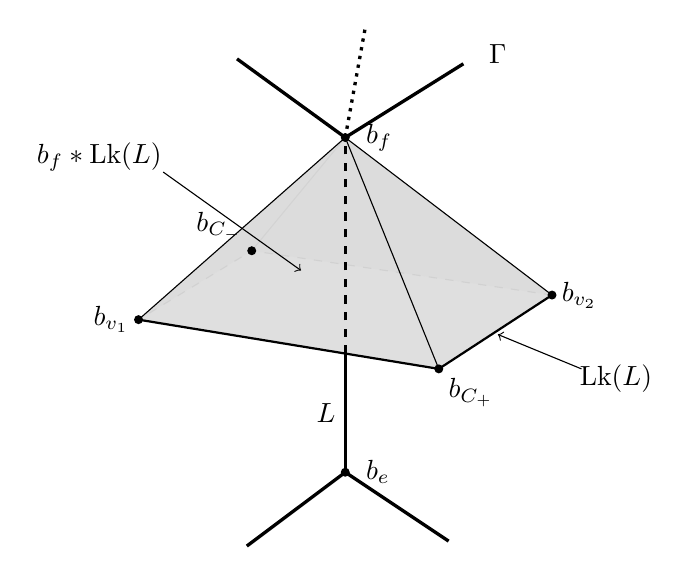
\begin{tikzpicture}[scale=1.25,line join=round]
\coordinate (be) at (0,-0.2);
\coordinate (bf) at (0,3.2);
\coordinate (v1) at (-2.1,1.35);
\coordinate (Cp) at (0.95,0.85);
\coordinate (v2) at (2.1,1.6);
\coordinate (Cm) at (-0.95,2.05);
\coordinate (cross) at (0,1.006);
\fill[gray!12] (bf) -- (v2) -- (Cm) -- cycle;
\fill[gray!12] (bf) -- (Cm) -- (v1) -- cycle;
\draw[gray!60] (bf) -- (Cm);
\draw[gray!70,dashed] (v2) -- (Cm) -- (v1);
\fill[gray!30,opacity=0.85] (bf) -- (v1) -- (Cp) -- cycle;
\fill[gray!30,opacity=0.85] (bf) -- (Cp) -- (v2) -- cycle;
\draw (bf) -- (v1); \draw (bf) -- (Cp); \draw (bf) -- (v2);
\draw[thick] (v1) -- (Cp) -- (v2);
\draw[very thick] (be) -- (cross);
\draw[very thick,dashed] (cross) -- (bf);
\draw[very thick] (bf) -- (-1.1,4.0);
\draw[very thick] (bf) -- (1.2,3.95);
\draw[very thick,dotted] (bf) -- (0.2,4.3);
\draw[very thick] (be) -- (-1.0,-0.95);
\draw[very thick] (be) -- (1.05,-0.9);
\foreach \p in {be,bf,v1,v2,Cp,Cm} \fill (\p) circle (1.3pt);
\node[right=4pt] at (be) {$b_e$};
\node[right=4pt] at (bf) {$b_f$};
\node[left] at (v1) {$b_{v_1}$};
\node[right] at (v2) {$b_{v_2}$};
\node[below right] at (Cp) {$b_{C_+}$};
\node[above left] at (Cm) {$b_{C_-}$};
\node[left] at (0,0.4) {$L$};
\node at (2.75,0.75) {$\cyLk(L)$};
\draw[->,thin] (2.4,0.85) -- (1.55,1.2);
\node at (-2.5,3.0) {$b_f*\cyLk(L)$};
\draw[->,thin] (-1.85,2.85) -- (-0.45,1.85);
\node at (1.55,4.05) {$\Gamma$};
\end{tikzpicture}
\caption{A leg $L=[b_e,b_f]$ of $\Gamma$, its link $\cyLk(L)$ in $\mathfrak K_0$, and the cone $b_f*\cyLk(L)$. The link passes
alternately through the vertex regions of the lower rays of the end points of $e$ and the open facets of the two maximal
cells containing $f$; with a coefficient $X\in\cyInv(A)$ its itinerary is the meridian class $\pm m_A(X)$. The cone meets
$\Gamma$ only at its apex $b_f$, where $X$ is a flat section.}\label{fig:meridian}
\end{figure}

\begin{lemma}[the complement lemma]\label{lem:complement}
$\ker\deg=I_\Gamma$.
\end{lemma}

The lemma says that every degree-zero class in the complement is generated by meridians with invariant coefficients.
The constant-coefficient assertion follows from $H_1(B;\Z)=0$. For the local system, the additional obstruction is
measured by the quotient of $N$ by the invariant lattices. Its two-cycles split into cochains on the graphs
$\Gamma\cap\partial F_u$. Since each $\partial F_u$ is a two-sphere, these cochains come from vertex functions.
Unimodularity then lifts the vertex functions to vectors in $N$ over the integers. These are the two steps of the proof
below; the last step is what excludes a finite-index obstruction.

\begin{proof}
Let $X_0$ be the two-dimensional cell complex obtained from the graph $G_0$ by attaching one square $\square_A$ for each arc
$A=C([u,u'],[n,n'])$ along the edge loop $(u,n),(u',n),(u',n'),(u,n')$. On $X_0$ consider the coefficient system $\hat\Lambda$
of subgroups of $N$ given by $u^\perp\cap N$ at the vertex $u$ and on the edges $(u,n)$, by $N$ at the vertex $n$, and by
$[u,u']^\perp\cap N$ on $\square_A$, with inclusions as restriction maps. Then $C_*(X_0;\hat\Lambda)$ is a subcomplex of
$C_*(X_0)\otimes N$. Its $1$-cycles are the $x$ with $\sum_nx_{un}=0$ and $\sum_ux_{un}=0$ in $N$, which is $\ker\deg$ because
$n\ne0$; and with suitable orientations of the squares $\partial(X\cdot \square_A)=m_A(X)$, so its $1$-boundaries form $I_\Gamma$. The
claim is $H_1(X_0;\hat\Lambda)=0$. Let $\mathcal Q=N/\hat\Lambda$. It is $0$ at the vertices $n$; $N/(u^\perp\cap N)\cong\Z$ by
$\langle u,\cdot\rangle$ at $u$ and on the edges $(u,n)$; and $N/([u,u']^\perp\cap N)\cong\Z^2$ by $(\langle u,\cdot\rangle,
\langle u',\cdot\rangle)$ on $\square_A$, these maps being onto because $u$, $u'$ are part of a basis of $M$
(Lemma~\ref{lem:stalks}(3)). The exact sequence of $0\to\hat\Lambda\to N\to\mathcal Q\to0$ contains
\[
H_2(X_0;N)\to H_2(X_0;\mathcal Q)\to H_1(X_0;\hat\Lambda)\to H_1(X_0;N),
\]
and we show that the last group vanishes and the first map is onto.

(a) $H_1(X_0;N)=H_1(X_0;\Z)\otimes N$ since $N$ is free, and $H_1(X_0;\Z)$ is the quotient of $H_1(G_0;\Z)$ by the classes of
the attaching loops. Lemma~\ref{lem:nerve}, with $\Lambda$ replaced by the constant system $\Z$, identifies
$H_1(B\setminus\Gamma;\Z)$ with $H_1(G_0;\Z)$, and carries the class of $\cyLk(L)$, $L\subset A$, to $\pm$ the attaching loop of
$\square_A$. So it suffices that the meridians $\cyLk(L)$ generate $H_1(B\setminus\Gamma;\Z)$. Let $U\supset\Gamma$ be the
neighbourhood of Section~\ref{ssec:normal} for $\mathfrak K=\mathfrak K_0$, and $\mathfrak E$ the union of the simplices of
$\mathfrak K_0'$ disjoint from $\Gamma$; then $B=U\cup \mathfrak E$, $U\cap \mathfrak E=\partial U$, and $B\setminus\Gamma$ retracts onto $\mathfrak E$ as
above. In the Mayer--Vietoris sequence $H_1(\partial U)\to H_1(U)\oplus H_1(\mathfrak E)\to H_1(B)=0$, a class $(0,\gamma)$ is the image
of a class of $H_1(\partial U)$ that vanishes in $H_1(U)$, that is, of a boundary $\partial\vartheta$, $\vartheta\in H_2(U,\partial U;\Z)$.
By Lemma~\ref{lem:nbhd}(3), $\vartheta$ is a sum of discs $\bar D(L)$, $L$ a leg, so $H_1(\mathfrak E)$ is generated by the circles
$\partial\bar D(L)$. The closed star $L*\cyLk(L)$ of $L$ in $\mathfrak K_0$ meets $\Gamma$ only in $L$, because $\Gamma$ is full,
and the radial projection along the join lines is a deformation retraction of $(L*\cyLk(L))\setminus L$ onto $\cyLk(L)$. It maps
$\partial\bar D(L)$, which lies in $(L*\cyLk(L))\setminus L$, homeomorphically onto $\cyLk(L)$: it sends the barycentre of $L*s$ to
the barycentre of $s$, and the segment between two such barycentres onto a segment. Hence $[\partial\bar D(L)]=\pm[\cyLk(L)]$ in
$H_1(B\setminus\Gamma)$.

(b) There are no three-cells, so $H_2(X_0;\mathcal Q)$ is the group of $2$-cycles. A $2$-chain with coefficients in $\mathcal Q$ is a
family of integers $p=(p^{(u)}_A)$, one for each arc $A$ and each vertex $u$ of $\tau_A$, where $A=C(\tau_A,\omega_A)$; the
boundary of $C_*(X_0;\mathcal Q)$ in degree two decouples over $u$, the component on the edge $(u,n)$ involving only the
$p^{(u)}$. Fix $u$ and let $S_u=\partial F_u$, a two-sphere oriented as the boundary of $F_u$. By (D2), $S_u$ is the union
of the cells $C(\tau,\omega)$ with $u\in\tau$ and $\dim\tau\ge1$, a subcomplex of the dual-pair complex. Its cells in $\Gamma$
form the graph $\Gamma_u=\Gamma\cap S_u$, whose one-cells are the arcs $A$ with $u\in\tau_A$; its other cells are the
$C(\tau,n)$, which group, according to $n$, into the sets $D^u_n=S_u\cap\widetilde R_n$. Each nonempty $D^u_n$ is connected:
its cells are the $C(u*\sigma,n)$, $\sigma$ a simplex of the link of $u$ in the triangulation of the face $n^\vee$ of
$\Delta^\circ$, with $C(u*\sigma,n)$ in the closure of $C(u*\sigma',n)$ when $\sigma\supseteq\sigma'$. That link is
connected: $n^\vee$ is a facet of $\Delta^\circ$ if $n$ is a vertex of $\Delta$, an edge of lattice length one (with $u$ an end
point) if $n$ is the centre of a pentagon or hexagon, and a point if $n$ lies in the interior of a facet of $\Delta$, and the
link of a vertex in a triangulated three-polytope is a disc or a sphere. So the $D^u_n$ are the components of
$S_u\setminus\Gamma_u$. An arc
$A=C([u,u'],[n,n'])$ lies in the closure of exactly two two-cells of $S_u$, $C([u,u'],n)\subseteq D^u_n$ and
$C([u,u'],n')\subseteq D^u_{n'}$, with opposite incidences; the two-face $F_{uu'}$ is oriented oppositely as a face of
$S_u$ and of $S_{u'}$, so the orientation of $\square_A$ can be chosen so that, for both $u$ and $u'$, the coefficient of
$\partial(p\,\square_A)$ on $(u,n)$ is $p$ times the incidence of $C([u,u'],n)$ with $A$ in $S_u$. With this choice, $p$ is a cycle
if and only if, for every $u$ and $n$, the $1$-cochain $p^{(u)}$ on the arcs of $\Gamma_u$ satisfies
\[
\sum_{\text{two-cells }f\subseteq D^u_n}\bigl(\delta\tilde p^{(u)}\bigr)(f)=0,
\]
where $\tilde p^{(u)}$ extends $p^{(u)}$ by zero to the one-cells of $S_u$ not in $\Gamma_u$ and $\delta$ is the cellular
coboundary of $S_u$.

Consider the exact sequence $0=H^1(S_u)\to H^1(\Gamma_u)\to H^2(S_u,\Gamma_u)$. The relative cellular cochains of
$(S_u,\Gamma_u)$ split as $\bigoplus_nC^*_n$, the cochains on the cells of $D^u_n$, since the coboundary of a cell $C(\tau,n)$
consists of cells $C(\tau',n)$. Each one-cell of $D^u_n$ lies on exactly two two-cells, both in $D^u_n$, with opposite
incidences, and $D^u_n$ is connected, so the sum of the values on the two-cells identifies $C^2_n/\delta C^1_n$ with $\Z$;
thus $H^2(S_u,\Gamma_u)=\bigoplus_n\Z$, and the connecting map sends the class of $p^{(u)}$ to the family of sums displayed
above. Therefore the $u$-components of $2$-cycles are exactly the coboundaries $p^{(u)}=\delta\varphi_u$ of functions
$\varphi_u$ on the vertices of $\Gamma_u$, that is, the integral combinations $\sum_v\varphi_u(v)\,\delta_u[v]$ of the vertex
cochains $\delta_u[v]$, which are $\pm1$ on the arcs of $\Gamma_u$ at $v$ and $0$ elsewhere (arcs have distinct end points).

For a $\Gamma$-vertex $v=C(\tau_v,\omega_v)$ let $\Sigma_v$ be the sum of the squares $\square_A$ of the arcs at $v$, with signs
making it a $2$-cycle of $X_0$ with integer coefficients: at a negative vertex or node the arcs are the $C(\tau_v,\varepsilon)$,
$\varepsilon$ an edge of $\omega_v$, and each edge $(u,n)$, $n$ a vertex of $\omega_v$, occurs in the two squares of the edges of
$\omega_v$ at $n$; at a positive vertex the arcs are the $C(\tau_1,\omega_v)$, $\tau_1$ an edge of $\tau_v$, and each edge
$(u,n)$ occurs in the two squares of the edges of $\tau_v$ at $u$. For $y\in N$ the image of $y\cdot\Sigma_v$ in
$C_2(X_0;\mathcal Q)$ has $u$-component, for $u\in\tau_v$, equal to $\langle u,y\rangle$ times a cycle supported on the arcs of
$\Gamma_u$ at $v$ with entries $\pm1$. The cycles supported on these arcs form a group of rank at most one. Indeed, the arcs of
$\Gamma_u$ at $v$ are the $C(\tau_1,\omega_1)$ at $v$ with $u\in\tau_1$; for such a cycle the condition attached to $D^u_n$
involves exactly the arcs at $v$ whose lower support contains $n$, each with coefficient $\pm1$; and the graph on the arcs at
$v$ in which two are joined when their lower supports share a vertex is connected (a cycle for a negative vertex or node, and
two arcs with the same lower support for a positive vertex). So the value on one arc determines the others. As $\delta_u[v]$ is such a cycle with entries $\pm1$, the $u$-component of the
image of $y\cdot\Sigma_v$ is $\epsilon_u(v)\langle u,y\rangle\,\delta_u[v]$ with $\epsilon_u(v)=\pm1$.

Now let $p$ be a $2$-cycle, $p^{(u)}=\sum_v\varphi_u(v)\,\delta_u[v]$. By Lemma~\ref{lem:stalks}(3) the map $N\to\Z^{\tau_v}$,
$y\mapsto(\langle u,y\rangle)_{u\in\tau_v}$, is onto, so there are $y_v\in N$ with $\langle u,y_v\rangle=\epsilon_u(v)\varphi_u(v)$ for
all $u\in\tau_v$. Then $\sum_vy_v\cdot\Sigma_v\in H_2(X_0;N)$ maps to $p$. So $H_2(X_0;N)\to H_2(X_0;\mathcal Q)$ is onto, and
$H_1(X_0;\hat\Lambda)=0$.
\end{proof}

\begin{theorem}[filling]\label{thm:filling}
$\partial Z(\mathfrak K_0)=\cyBal$.
\end{theorem}

\begin{proof}
$\partial Z(\mathfrak K_0)\subseteq\cyBal$ because $\partial\partial=0$. Let $\beta\in\cyBal$ and let $\zeta$, $b$, $\theta$, $b'$ be as in
Steps~1 and~2. By Lemmas~\ref{lem:nerve} and~\ref{lem:complement}, $\cyit[b']\in\ker\deg=I_\Gamma$, so
$\cyit[b']=\sum_i m_{A_i}(X_i)$ for finitely many arcs $A_i$ and $X_i\in\cyInv(A_i)$. Choose a leg $L_i\subset A_i$ with
apex $b_{f_i}$, and signs so that $\cyit[X_i\cdot\cyLk(L_i)]=m_{A_i}(X_i)$. Then $b'-\sum_iX_i\cdot\cyLk(L_i)$ is a $1$-cycle on
$\mathfrak K_0^\circ$ with itinerary zero, hence null-homologous in $B\setminus\Gamma$ (Lemma~\ref{lem:nerve}), hence the boundary
$\partial y_0$ of a $2$-chain $y_0$ on $\mathfrak K_0^\circ$ with coefficients in $\Lambda$. Put
\[
z:=\zeta-\theta+y_0+\sum_iX_i\cdot\bigl(b_{f_i}*\cyLk(L_i)\bigr)\in C_2(\mathfrak K_0;F).
\]
Since $\beta=b+\partial\zeta$, $b=b'-\partial \theta$, $b'=\partial y_0+\sum_iX_i\cdot\cyLk(L_i)$ and $\partial(b_f*c)=c$ for a $1$-cycle
$c$, we get $\partial z=\beta$. So $z\in Z(\mathfrak K_0)$ with boundary network $\beta$.
\end{proof}

\begin{proof}[Proof of Theorem~\ref{thm:real}]
By Theorem~\ref{thm:filling} and Proposition~\ref{prop:rhoH},
\[
\rho(Z(\mathfrak K_0))=\rho(\partial Z(\mathfrak K_0))=\rho(\cyBal)=K.
\]
For any triangulation $\mathfrak K$ of $B$ in which $\Gamma$ is full, $\partial Z(\mathfrak K)\subseteq\cyBal$
(Section~\ref{ssec:coef}), so $\rho(Z(\mathfrak K))\subseteq K$.
\end{proof}

If $\mathfrak K$ is a subdivision of $\mathfrak K_0$ in which $\Gamma$ is full, the subdivision operator carries $Z(\mathfrak K_0)$
into $Z(\mathfrak K)$ without changing node coefficients, so $\rho(Z(\mathfrak K))=K$ as well.

\begin{remark}[no torsion]\label{rem:notorsion}
Every step is integral: $H_1(D_\varepsilon,\partial D_\varepsilon)=0$, $H_1(\mathcal X)=0$, $H^1(S^2)=0$, $H_1(S^3)=0$, and the
unimodularity of $\mathcal T$ in Lemma~\ref{lem:stalks}(3). No condition on the torsion of $H_2(\widehat X;\Z)$ or of
$H_1(B;\iota_*\Lambda)$ enters, and $\rho(Z(\mathfrak K_0))$ is $K$ itself, not a sublattice of finite index.
\end{remark}

\begin{remark}[where $K$ enters]\label{rem:whereK}
The lattice $K$ enters only through Proposition~\ref{prop:rhoH}. Theorem~\ref{thm:filling} holds for every balanced network,
whatever its node coefficients, and its proof uses Hypothesis~\ref{hyp:P} only through the existence of $B$, admissibility
through the list of $\Gamma$-vertices (D3), and Theorem~\ref{thm:U} through Lemma~\ref{lem:stalks}(2),(3). The fillings it
constructs consist of sheets $\zeta_\varepsilon\otimes d_\varepsilon$ in the dual discs, with coefficients in $\Z d_\varepsilon$ and
containing arcs and positive vertices in their interior; pairs of triangles at the $\Gamma$-points of the dual paths, with
coefficients in $\cylin(\omega)$; cones $b_f*\cyLk(L)$ crossing a leg at $b_f$ with an invariant coefficient; and a
$\Lambda$-valued $2$-chain in $B\setminus\Gamma$. The finite computations illustrating the theorem are described in Section~\ref{ssec:list}.
\end{remark}

\part{The mirror lift and the relation lattice}
\section{The transfer to the mirror base}\label{sec:legendre}

The relative tropical $2$-cycles of Theorem~\ref{thm:real} live on the base $B'_\sigma$, whereas the chains of
Theorem~\ref{thm:lift} are built over the base $B_Y$ of the degeneration of the mirror family. This section constructs a
piecewise linear homeomorphism $\mathfrak h\colon B'_\sigma\to B_Y$ that carries the discriminant of $B'_\sigma$ onto that of
$B_Y$ and the local system of integral tangent vectors of $B'_\sigma$ onto the dual of that of $B_Y$, and uses it to
transfer relative tropical $2$-cycles to $B_Y$ with the same boundary networks and the same node coefficients
(Proposition~\ref{prop:transfer}). The homeomorphism is assembled from three comparisons, each compatible with the
dual-pair complex of Section~\ref{sec:dualpair}: a change of fan-side subdivision (Proposition~\ref{prop:F}), by which $\Sigma'$ is
replaced by $\mathcal F_C$; a change of height (Lemma~\ref{lem:height}); and the dual-pair homeomorphism between the two bases built
from the same data (Proposition~\ref{prop:L1}). Lemmas~\ref{lem:D} and~\ref{lem:arc} describe the cell structure near a
node and near an arc of the discriminant; these are the neighbourhoods in which the local models of Section~\ref{sec:lift}
are placed.

\subsection{Change of fan-side subdivision and of height}\label{ssec:leg-F}
Three comparisons of bases occur in this paper: a change of fan-side subdivision (Proposition~\ref{prop:F}), a change of height
(Lemma~\ref{lem:height}) and the passage to the mirror base (Section~\ref{ssec:leg-transfer}). Each consists of a
piecewise linear homeomorphism of pairs and an isomorphism of local systems, and each carries relative tropical
$2$-cycles by the following lemma.

\begin{lemma}[transport of relative cycles]\label{lem:transport}
For $i=1,2$ let $B_i$ be a closed piecewise linear three-manifold, $\Gamma_i\subset B_i$ a compact one-dimensional
subpolyhedron, $\Lambda_i$ a local system of free abelian groups of rank three on $B_i\setminus\Gamma_i$, and suppose that
$\Gamma_i$ is the union of finitely many points and open arcs $A$, each carrying a flat section $d_A$ of $\Lambda_i$ over
$V_A\setminus\Gamma_i$ for a neighbourhood $V_A$ of the closure $\bar A$. For triangulations
$\mathfrak K$ of $B_i$ in which $\Gamma_i$ is a full subcomplex define $F_i$, $\mathcal D_i(E)=\Z d_A$ for $E\subseteq A$,
and $Z_i(\mathfrak K)$ as in Definition~\ref{def:relcycle}. Let $f\colon B_1\to B_2$ be a piecewise linear homeomorphism
with $f(\Gamma_1)=\Gamma_2$, mapping each arc $A$ onto an arc $f(A)$, and $\theta\colon\Lambda_1\to f^*\Lambda_2$ an
isomorphism of local systems on $B_1\setminus\Gamma_1$ with $\theta(d_A)=d_{f(A)}$ for every arc $A$. Let $\mathfrak K$ be a
triangulation of $B_1$ in which $\Gamma_1$ is full, $\mathfrak K^0_1$ a subdivision of $\mathfrak K$ on whose simplices $f$
is linear, and $\mathfrak K_1$ a derived subdivision of $\mathfrak K^0_1$. Then:
\begin{enumerate}
\item $f(\mathfrak K_1)$ is a triangulation of $B_2$ in which $\Gamma_2$ is a full subcomplex; if $f$ is linear on the
simplices of $\mathfrak K$, the same holds for $f(\mathfrak K)$, and one may take $\mathfrak K_1=\mathfrak K$ below;
\item $\theta$ induces isomorphisms $F_1(s)\to F_2(f(s))$, compatible with the restrictions and carrying $\mathcal
D_1(E)$ onto $\mathcal D_2(f(E))$, hence an isomorphism of chain complexes $f_\#\colon C_*(\mathfrak K_1;F_1)\to
C_*(f(\mathfrak K_1);F_2)$ mapping $C_*(\Gamma_1;\mathcal D_1)$ onto $C_*(\Gamma_2;\mathcal D_2)$;
\item the composite $f_*:=f_\#\circ\lgsd\colon Z_1(\mathfrak K)\to Z_2(f(\mathfrak K_1))$, with $\lgsd$ the subdivision
operator, is an injective homomorphism, and if $\partial z=\sum_Ec_Ed_{A(E)}[E]$, $A(E)$ the arc containing the edge $E$,
then $\partial f_*z=\sum_Ec_E\sum_{E'\subseteq E}d_{f(A(E))}[f(E')]$, the inner sum over the edges $E'$ of $\mathfrak K_1$
in $E$ with the orientation of $E$.
\end{enumerate}
\end{lemma}

\begin{proof}
(1) The subcomplex $\Gamma_1$ of $\mathfrak K$ is a subcomplex of every subdivision, and in a derived subdivision every
subcomplex is full \cite[Ch.~3]{RS}. As $f$ is linear on the simplices of $\mathfrak K_1$, it is a simplicial isomorphism
onto $f(\mathfrak K_1)$, which is therefore a triangulation of $B_2$ with $\Gamma_2=f(\Gamma_1)$ full. The derived
subdivision is needed: in an arbitrary subdivision on which $f$ is linear, a simplex with all its vertices on $\Gamma_1$
need not lie in $\Gamma_1$.

(2) For a simplex $s$ of $\mathfrak K_1$, $f$ maps the neighbourhoods $V$ of $\bar s$ onto neighbourhoods $f(V)$ of
$f(\bar s)$, all small ones arising in this way, with $f(V\setminus\Gamma_1)=f(V)\setminus\Gamma_2$, and $\theta$ maps the
flat sections of $\Lambda_1$ over $V\setminus\Gamma_1$ to the flat sections of $\Lambda_2$ over $f(V)\setminus\Gamma_2$,
compatibly with restriction to smaller sets. By hypothesis it carries $d_A$ to $d_{f(A)}$.

(3) The subdivision operator sends an oriented simplex $s$ of $\mathfrak K$ with coefficient $X\in F(s)$ to the sum of the
simplices $s'$ of $\mathfrak K_1$ of the same dimension in $\bar s$, with the induced orientations and the coefficients
$X|_{s'}$; the restriction is defined because a neighbourhood of $\bar s$ is a neighbourhood of $\bar s'$. It is a chain
map, it maps $C_*(\Gamma_1;\mathcal D_1)$ into itself, since the edges of $\mathfrak K_1$ in an edge $E\subseteq A$ of
$\Gamma_1$ lie in $A$, and it is injective, since restriction of flat sections to a smaller connected set is injective and
$V\setminus\Gamma_1$ is connected for small $V$. So it maps $Z_1(\mathfrak K)$ injectively into $Z_1(\mathfrak K_1)$, with
the stated boundary, and (2) applies.
\end{proof}

\begin{proposition}[change of fan-side subdivision]\label{prop:F}
Let $\mathcal F_1$ and $\mathcal F_2$ be two fan-side subdivisions which agree on the two-skeleton of $\partial\Delta$: a cell of either
contained in a face of $\Delta$ of dimension at most two is a cell of the other. Write $C^i$, $\Gamma^i_X$, $\Lambda^i_X$ for
the cells, discriminant and local system of $B_X(\mathcal F_i)$; the underlying space $\partial\nabla^{\check h}$ is the
same.
\begin{enumerate}
\item The dual pairs $(\tau,\omega)$ with $\dim\tau\ge1$ are the same for $\mathcal F_1$ and $\mathcal F_2$.
\item If $\omega$ is not contained in a face of $\Delta$ of dimension at most two, then every dual pair $(\tau,\omega)$ has
$\tau=\{u_G\}$, where $G$ is the facet of $\Delta$ containing $\omega$ and $u_G$ the vertex of $\Delta^\circ$ dual to $G$.
\item There is a piecewise linear homeomorphism $g$ of $\partial\nabla^{\check h}$, preserving every face $F_\tau$ and
isotopic to the identity through face-preserving homeomorphisms, such that $g(C^1(\tau,\omega))=C^2(\tau,\omega)$
for $\dim\tau\ge1$. In particular $g(\Gamma^1_X)=\Gamma^2_X$, $g$ maps the arc $C^1([u,u'],[n,n'])$ onto the arc
$C^2([u,u'],[n,n'])$ and each vertex of $\Gamma^1_X$ onto the vertex of $\Gamma^2_X$ of the same dual pair, and there is an
isomorphism $\kappa\colon\Lambda^1_X\to g^*\Lambda^2_X$ that is the identity of $u^\perp\cap N$ on every open facet
$\operatorname{int}F_u$ and carries the vanishing vector $n'-n$ of each arc to that of its image.
\item If $h_1$ and $h_2$ agree on the lattice points of the two-skeleton, $g$ can be taken to be the identity on the
two-skeleton of $\partial\nabla^{\check h}$.
\end{enumerate}
\end{proposition}
\begin{proof}
(1) If $\dim\tau\ge1$, then $\omega\subseteq\tau^\vee$, a face of $\Delta$ of dimension at most two, where the two
subdivisions agree. (2) The smallest face of $\Delta$ containing $\omega$ is a facet $G$, and $\tau^\vee$ is a proper face
of $\Delta$ containing $\omega$, so $\tau^\vee=G$; the only point $m\in\Delta^\circ$ with $\langle m,\cdot\,\rangle=-1$ on
$G$ is $u_G$.

(3) By Proposition~\ref{prop:L1}(5), the two-skeleton $\bigcup_{\dim\tau\ge1}F_\tau$ is the union of the cells
$C^i(\tau,\omega)$ with $\dim\tau\ge1$; these form a subcomplex of each dual-pair complex, with the same indexing set and
order by (1). The inductive construction in the proof of Proposition~\ref{prop:L1}(4), applied to these two regular CW
structures on the same space, gives a piecewise linear homeomorphism $g$ of the two-skeleton with
$g(C^1(\tau,\omega))=C^2(\tau,\omega)$; it preserves every $F_\tau$ with $\dim\tau\ge1$, which is the union of the cells
$C^i(\tau',\omega)$ with $\tau'\supseteq\tau$. Extend $g$ over each facet, a convex three-ball whose boundary it preserves,
by coning from an interior point; the cone of a piecewise linear map is piecewise linear. Faces of dimension zero are
points and are fixed; on the edges, the two-faces and the facets in turn, $g$ is isotopic to the identity relative to the
lower-dimensional faces by the Alexander trick, extended by coning as in Appendix~\ref{app:leg-pl}. By
Propositions~\ref{prop:L2}(1),(2), $g(\Gamma^1_X)=\Gamma^2_X$, with arcs and vertices as stated. Define $\kappa$ on each
$\operatorname{int}F_u$, which $g$ preserves, as the identity of $u^\perp\cap N$. A point $b$ of the two-skeleton outside
$\Gamma^1_X$ lies in some $C^1(\tau,n)$ with $\dim\tau\ge1$, so $b\in\widetilde R^1_n$ and $g(b)\in C^2(\tau,n)\subseteq
\widetilde R^2_n$. On a connected neighbourhood $U\subseteq\widetilde R^1_n\cap g^{-1}(\widetilde R^2_n)$ of $b$ both local
systems are the constant $N/\Z n$, and on $U\cap\operatorname{int}F_u$ the identity of $u^\perp\cap N$ corresponds to the
identity of $N/\Z n$ under $\pi^X_{un}$ on both sides. So $\kappa$ extends over $U$ as the identity of $N/\Z n$, compatibly
on overlaps, and is an isomorphism of local systems on $\partial\nabla^{\check h}\setminus\Gamma^1_X$. Near the arc
$C^i([u,u'],[n,n'])$ the vanishing vector is represented in the chart of $F_u$ by $n'-n\in u^\perp\cap N$ on both bases
(Proposition~\ref{prop:L2}(4)), and $\kappa$ is the identity there.

(4) By Lemma~\ref{lem:cayley}(2), the decomposition of a face $F_\tau$ with $\dim\tau\ge1$ depends only on the restriction
of $h_i$ to $\tau^\vee\cap N$, which lies in the two-skeleton of $\partial\Delta$. So the two decompositions, their
barycentric subdivisions and their cells agree on the two-skeleton, and $g$ can be taken to be the identity there.
\end{proof}

The vertices of $\mathcal F_2$ in the interior of a facet $G$ of $\Delta$ only change the cells $C^2(u_G,\omega)$ inside the
open facet $\operatorname{int}F_{u_G}$, by (2); there $\Lambda^2_X$ is the constant facet lattice, and $\kappa$ is its
identity.

We apply Proposition~\ref{prop:F} with $\mathcal F_1=\Sigma'$ and $\mathcal F_2=\mathcal F_C$. The pulling refinement
$\mathcal F_C$ is a fan-side subdivision, induced by the height $h_C$, and it agrees with $\Sigma'$ on the two-skeleton
(Proposition~\ref{prop:pulling}). We build $B_X(\mathcal F_C)$ with the function $h_C$, and fix the resulting piecewise
linear homeomorphism $g_C\colon B'_\sigma\to B_X(\mathcal F_C)$ and the isomorphism $\kappa_C\colon\Lambda\to g_C^*\Lambda^{\mathcal F_C}_X$. Since $g_C$ maps the vertex $p_q$ of the discriminant,
the zero-cell $C([u,u'],P_q)$, to the zero-cell of the same dual pair, and each arc to the arc with the same lower support,
the node coefficients of Definition~\ref{def:nodecoef}, read from the lower supports of the legs at $p_q$, are preserved by
the transport $(g_C)_*$ of Lemma~\ref{lem:transport}.

\begin{remark}\label{rem:gCid}
If every lattice point of $\partial\Delta$ is a vertex of $\Sigma'$, no point is pulled and $\mathcal F_C=\Sigma'$; if in
addition $B_X(\mathcal F_C)$ is built with the same function $h$ as $B'_\sigma$, then $g_C$ can be taken to be the identity.
This is the case for the subdivisions of the examples of Section~\ref{sec:examples}. Nothing in this paper uses it.
\end{remark}

\begin{lemma}[change of height]\label{lem:height}
Let $\check h_1$ and $\check h_2$ be two integral heights on the same unimodular triangulation $\mathcal T$ of
$\partial\Delta^\circ$, both with $\check h_i$ and $\check h_i-\check\varphi$ strictly convex on the fan over $\mathcal T$, and
let $B_i=\partial\nabla^{\check h_i}$ be the base $B_X(\Sigma')$ built from $\check h_i$, with the same function $h$ in
$\widetilde\Sigma'$. Write $C^i(\tau,\omega)$ for the cells of its dual-pair complex, $\Gamma_i$ for its discriminant and
$\Lambda_i$ for its local system. Then:
\begin{enumerate}
\item there is a piecewise linear homeomorphism $\phi\colon B_1\to B_2$ with $\phi(C^1(\tau,\omega))=C^2(\tau,\omega)$ for
every dual pair $(\tau,\omega)$; it maps each open facet $\operatorname{int}F_u$ and each region $\widetilde R_n$ onto the
open facet and the region with the same index, $\Gamma_1$ onto $\Gamma_2$, each vertex $p_q$ of the discriminant onto $p_q$, each arc onto
the arc with the same dual pair, and each vertex of $\Gamma_1$ onto a vertex of $\Gamma_2$ of the same type;
\item there is an isomorphism of local systems $\kappa\colon\Lambda_1\to\phi^*\Lambda_2$ on $B_1\setminus\Gamma_1$ that is the
identity of $u^\perp\cap N$ on every $\operatorname{int}F_u$ and the identity of $N/\Z n$ on every $\widetilde R_n$;
\item the transport $\phi_*$ of Lemma~\ref{lem:transport} carries relative tropical $2$-cycles on $B_1$ to relative
tropical $2$-cycles on $B_2$ with the same integers $c_E$ in their boundary networks and the same node coefficients; and
$(S,j,v)\mapsto(S,\phi\circ j,\kappa(v))$ is a bijection from the tropical $2$-cycles of \cite[Def.~7.2]{CBM} on $B_1$ to
those on $B_2$, which preserves piecewise linearity of $j$ and the node coefficients.
\end{enumerate}
In particular, relative tropical $2$-cycles and tropical $2$-cycles on the base of any such height on $\mathcal T$ are
carried to cycles of the same kind on the base of the normalised height of Section~\ref{ssec:gross}, with the same node
coefficients.
\end{lemma}
\begin{proof}
(1) The homeomorphism of Lemma~\ref{lem:indepheight} has these properties. Alternatively: the set of dual pairs and its order depend only on $\mathcal T$ and $\Sigma'$, and Proposition~\ref{prop:L1}, which
uses only the strict convexity of $\check h_i$ and $\check h_i-\check\varphi$, applies to both heights. The inductive
construction in its proof gives piecewise linear homeomorphisms $\Psi_i\colon|\lgOrd(\lgDP)|\to B_i$ with
$\Psi_i(|\lgOrd^{\preceq {\mathfrak p}}|)=\overline{C^i({\mathfrak p})}$, and $\phi=\Psi_2\circ\Psi_1^{-1}$ preserves the cells. The facets, regions,
arcs and vertices of the discriminant are unions of cells described by their dual pairs (Propositions~\ref{prop:L1}(5)
and~\ref{prop:L2}(1),(2)); the vertex $p_q$ of the discriminant is the zero-cell $C^i([u,u'],P_q)$, the barycentre of the carrying cell, the
unique cell with face label $[u,u']$ and lower support $P_q$ (Lemma~\ref{lem:stack}); and the type of a three-valent vertex
is determined by its dual pair (Proposition~\ref{prop:L2}(3)).

(2) The open facets and the regions cover $B_i\setminus\Gamma_i$, with $\operatorname{int}F_u\cap\widetilde R_n=C^i(u,n)$
and no triple intersections (proof of Proposition~\ref{prop:L3}). On $\operatorname{int}F_u$ the lattice $\Lambda_i$ is
$u^\perp\cap N$, on $\widetilde R_n$ it is $N/\Z n$, and on $C^i(u,n)$ the two are related by the projection
$u^\perp\cap N\to N/\Z n$, on both bases. So the identities on the pieces agree on the overlaps and define $\kappa$.

(3) The pair $(\phi,\kappa)$ satisfies the hypotheses of Lemma~\ref{lem:transport}: near the arc of $([u,u'],[n,n'])$ the
vanishing vector is $n'-n\in u^\perp\cap N$ on both bases and $\kappa$ is the identity there. The integers $c_E$ are
therefore unchanged, and the node coefficients, read from the lower supports of the legs at the node points
(Definition~\ref{def:nodecoef}), are unchanged by (1). The clauses of \cite[Def.~7.2]{CBM} refer to the topology of $S$
and $j$, to $\Gamma_i$ with its vertex types and nodes, and to $\Lambda_i$ and its monodromy. An orientation of $B_i$ enters
only through Definition~\ref{def:types}, and the types do not depend on it (Remark~\ref{rem:sameloop}). By (1) and (2),
$\phi$ and $\kappa$ preserve all of these, and $\kappa$ intertwines parallel transport, so $(S,\phi\circ j,\kappa(v))$
satisfies the clauses if and only if $(S,j,v)$ does; $\phi\circ j$ is piecewise linear if $j$ is. For a tropical
$2$-cycle, triangulated, the node coefficients are those of the relative cycle it defines (Section~\ref{ssec:cbm}), and
these are unchanged.
\end{proof}

\subsection{The node star and the neighbourhood of an arc}\label{ssec:leg-node}
In this subsection $B_X=B_X(\mathcal F_C)$, $B_Y$ is the mirror base, and $\mathcal L=\Psi_Y\circ\Psi_X^{-1}$ is the
dual-pair homeomorphism constructed in the proof of Proposition~\ref{prop:L1}(4), which we fix. Since $g_C$ preserves the faces of
$\partial\nabla^{\check h}$ and the cells $C(\tau,\omega)$ with $\dim\tau\ge1$ (Proposition~\ref{prop:F}(3)), statements
about $B'_\sigma$ that involve only these are carried over by $g_C$.

Let $q\in Q$ be a node, with node parallelogram $P=abcd$ in the two-face $G$ of $\Delta$, labelled as in
Section~\ref{ssec:admissible}, and $G^\circ=[u,u']$, an edge of $\mathcal T$ because $\ell(G^\circ)=1$. Then
$([u,u'],P)$ is a dual pair of dimension zero; its zero-cell in $B'_\sigma$ is the vertex $p_q$ of the discriminant, the barycentre of the
carrying cell, the unique cell of $\mathscr P$ with face label $[u,u']$ and lower support $P$ (Lemma~\ref{lem:stack}).
Write ${\mathfrak q}=([u,u'],P)$ for this dual pair; its zero-cells are indexed by the node $q$. Put $f_1=b-a=c-d$ and $f_2=d-a=c-b$. The statements
below concern only the cells of $\mathcal T$ contained in $[u,u']$ and the cells of $\mathcal F_C$ contained in $P$; they do
not depend on whether $G$ is a square, a pentagon or a hexagon, nor, for a hexagon, on the branch of the profile.

To a face $\omega$ of $P$ assign $(\epsilon_1(\omega),\epsilon_2(\omega))\in\{-,0,+\}^2$, its position in the directions
$f_1$ and $f_2$: $a\mapsto(-,-)$, $b\mapsto(+,-)$, $c\mapsto(+,+)$, $d\mapsto(-,+)$, $ab\mapsto(0,-)$, $bc\mapsto(+,0)$,
$cd\mapsto(0,+)$, $da\mapsto(-,0)$, $P\mapsto(0,0)$. To $\tau\in\{u,[u,u'],u'\}$ assign $\epsilon_3(u)=-$,
$\epsilon_3([u,u'])=0$, $\epsilon_3(u')=+$. In $\R^3$ with coordinates $(y_1,y_2,y_3)$ let
$\mathcal O_\epsilon=\{y:\operatorname{sign}y_i=\epsilon_i\}$ for $\epsilon\in\{-,0,+\}^3$, the relatively open coordinate
orthants of all dimensions, and $O=\{|y_1|+|y_2|+|y_3|\le1\}$. Put $\operatorname{St}^X_q=\Psi_X(\operatorname{st}{\mathfrak q})$ and
$\operatorname{St}^Y_q=\Psi_Y(\operatorname{st}{\mathfrak q})$, where $\operatorname{st}{\mathfrak q}$ is the closed star of the vertex ${\mathfrak q}$ in
$\lgOrd(\lgDP)$; these are closed neighbourhoods of the zero-cells indexed by $q$, and $\mathcal L(\operatorname{St}^X_q)=\operatorname{St}^Y_q$.
Finally let $\mathcal W_q$ be the union of the cells $C_Y([u,u'],\omega)$, $\omega\subseteq P$: the node, the four arcs at it
and the four two-cells between them.

\begin{lemma}[the node star]\label{lem:D}
\begin{enumerate}
\item The dual pairs ${\mathfrak p}\succeq{\mathfrak q}$ are the $27$ pairs $(\tau,\omega)$ with $\tau$ equal to $u$, $[u,u']$ or $u'$ and
$\omega$ a face of $P$: the node; four arcs, $\tau=[u,u']$ and $\omega$ an edge; four two-cells, $\tau=[u,u']$ and
$\omega$ a vertex; two one-cells, $\omega=P$ and $\tau$ a vertex; eight two-cells, $\tau$ a vertex and $\omega$ an edge;
and eight three-cells, $\tau$ and $\omega$ vertices. The map
$\epsilon(\tau,\omega)=(\epsilon_1(\omega),\epsilon_2(\omega),\epsilon_3(\tau))$ is an isomorphism of this poset onto the
face poset of the coordinate fan: ${\mathfrak p}\preceq {\mathfrak p}'$ if and only if $\mathcal O_{\epsilon({\mathfrak p})}\subseteq
\overline{\mathcal O_{\epsilon({\mathfrak p}')}}$; and $\dim{\mathfrak p}$ is the number of nonzero entries of $\epsilon({\mathfrak p})$.
\item There are piecewise linear homeomorphisms $\Phi^X_q\colon\operatorname{St}^X_q\to O$ and
$\Phi^Y_q\colon\operatorname{St}^Y_q\to O$ with $\Phi^X_q(C_X({\mathfrak p})\cap\operatorname{St}^X_q)=\mathcal O_{\epsilon({\mathfrak p})}\cap O=
\Phi^Y_q(C_Y({\mathfrak p})\cap\operatorname{St}^Y_q)$ for all ${\mathfrak p}\succeq{\mathfrak q}$, and $\Phi^Y_q\circ\mathcal L=\Phi^X_q$ on
$\operatorname{St}^X_q$. Any two homeomorphisms $\operatorname{St}^Y_q\to O$ with this property are isotopic through such
homeomorphisms.
\item Consequently $\Phi^Y_q(\mathcal W_q\cap\operatorname{St}^Y_q)=\{y_3=0\}\cap O$; $\Phi^Y_q$ maps
$\widetilde R^*_u\cap\operatorname{St}^Y_q$ and $\widetilde R^*_{u'}\cap\operatorname{St}^Y_q$ onto $\{y_3<0\}\cap O$ and
$\{y_3>0\}\cap O$, the open facets $\operatorname{int}F^*_a,\dots,\operatorname{int}F^*_d$ onto the four quadrants
$\{(\operatorname{sign}y_1,\operatorname{sign}y_2)=(\epsilon_1,\epsilon_2)\}$ of the vertices, and the edge $F^*_P$ of
$\nabla^H$ onto the $y_3$-axis. On $B_X$, $\Phi^X_q$ maps $F_{uu'}\cap\operatorname{St}^X_q$ onto $\{y_3=0\}\cap O$ and
$\operatorname{int}F_u$, $\operatorname{int}F_{u'}$ onto the two half-balls.
\end{enumerate}
\end{lemma}
\begin{proof}
(1) The pairs $\succeq{\mathfrak q}$ are the $(\tau,\omega)$ with $\tau\subseteq[u,u']$ and $\omega\subseteq P$, and every such pair is
dual, being contained in a dual pair. The faces of the parallelogram $P$ are the products of faces of two segments, and the
faces of the segment $[u,u']$ are its end points and itself; in each factor, inclusion of faces corresponds to
$\epsilon_i\in\{0,\epsilon'_i\}$ with $0$ for the larger face, which is the order of the coordinate fan. The number of
nonzero entries is $3-\dim\tau-\dim\omega$.

(2) The closed star of ${\mathfrak q}$ in $\lgOrd(\lgDP)$ consists of the chains containing ${\mathfrak q}$ and their subchains; since ${\mathfrak q}$ is
minimal in $\{{\mathfrak p}\succeq{\mathfrak q}\}$ and has $\dim{\mathfrak q}=0$, it is the cone ${\mathfrak q}*\lgOrd(\lgDP_{\succ{\mathfrak q}})$. The nonzero sign vectors, ordered
as in (1), form the face poset of the boundary of the cross-polytope $O$, the face of $\epsilon$ being
$\operatorname{conv}\{\epsilon_ie_i:\epsilon_i\ne0\}$; so $\epsilon$ induces a simplicial isomorphism of
$\lgOrd(\lgDP_{\succ{\mathfrak q}})$ with the barycentric subdivision of $\partial O$, whose cone is a piecewise linear homeomorphism
$E_q\colon|\operatorname{st}{\mathfrak q}|\to O$. The open simplices of $\operatorname{st}{\mathfrak q}$ whose chain has top ${\mathfrak p}$ are mapped onto
$\mathcal O_{\epsilon({\mathfrak p})}\cap O$, and $\Psi_X$ maps their union onto $C_X({\mathfrak p})\cap\operatorname{St}^X_q$, because open
simplices of chains with top ${\mathfrak p}$ lie in $\Psi_X^{-1}(C_X({\mathfrak p}))$. So $\Phi^X_q=E_q\circ\Psi_X^{-1}$ and
$\Phi^Y_q=E_q\circ\Psi_Y^{-1}$ have the stated properties, and $\Phi^Y_q\circ\mathcal L=\Phi^X_q$. Two homeomorphisms with
the property differ by a homeomorphism of $O$ preserving every $\mathcal O_\epsilon\cap O$, which is isotopic to the
identity through such homeomorphisms (Appendix~\ref{app:leg-pl}).

(3) The cells of $\mathcal W_q$ are those with $\tau=[u,u']$, that is, $\epsilon_3=0$. By
Proposition~\ref{prop:L1}(5), $\widetilde R^*_u\cap\operatorname{St}^Y_q$ is the union of the cells $C_Y(u,\omega)$, that
is, $\epsilon_3=-$; $\operatorname{int}F^*_a\cap\operatorname{St}^Y_q$ is the union of the cells $C_Y(\tau,a)$, that is,
$(\epsilon_1,\epsilon_2)=(-,-)$; and $F^*_P\cap\operatorname{St}^Y_q$ is the union of the cells $C_Y(\tau,P)$, that is,
$\epsilon_1=\epsilon_2=0$. On $B_X$, $F_{uu'}$ and $\operatorname{int}F_u$ are the unions of the cells with $\tau=[u,u']$,
respectively $\tau=u$, by Proposition~\ref{prop:L1}(5).
\end{proof}

The arcs at the node map under $\Phi^Y_q$ to the four half-axes in $\{y_3=0\}$: the arc over $ab$ to
$\{y_1=y_3=0,\ y_2<0\}$, over $dc$ to $y_2>0$, over $da$ to $y_1<0$ and over $bc$ to $y_1>0$. The four \emph{standard
halves} at $q$ are the sets $(\Phi^Y_q)^{-1}(\{y_1=0,\ \pm y_3\ge0\})$ and $(\Phi^Y_q)^{-1}(\{y_2=0,\ \pm y_3\ge0\})$; by (1)
and (3), $(\Phi^Y_q)^{-1}(\{y_1=0,\ y_3\ge0\})$ is the union of the closed cells with sign vectors $(0,\ast,+)$ and
$(0,\ast,0)$, that is, the closure of $C_Y(u',ab)\cup C_Y(u',P)\cup C_Y(u',cd)$, and similarly for the other three. In the
node model of Section~\ref{sec:regime}, the tropical chart $T_q$ of Lemma~\ref{lem:nodemodel}(4) has the same
quadrant and half-space description. That lemma compares the chart with scaled logarithmic coordinates on the
hypersurface up to $O(1/L)$; the cell identification here concerns the tropical bases.

Let ${\mathfrak p}_e=([u,u'],[n,n'])$ be a dual pair of edges, so that $C_Y({\mathfrak p}_e)$ is an arc of $\Gamma_Y$
(Proposition~\ref{prop:L2}(2)). To the faces of $[n,n']$ assign $\epsilon_1(n)=-$, $\epsilon_1(n')=+$,
$\epsilon_1([n,n'])=0$, and to the faces of $[u,u']$ assign $\epsilon_2(u)=-$, $\epsilon_2(u')=+$, $\epsilon_2([u,u'])=0$.
For $\epsilon\in\{-,0,+\}^2$ let $\mathcal O^{(2)}_\epsilon=\{(x_1,x_2):\operatorname{sign}x_i=\epsilon_i\}$. In $\R^3$ with
coordinates $(x_1,x_2,x_3)$ let $V=\operatorname{conv}\bigl((\Diamond\times\{0\})\cup\{\pm e_3\}\bigr)$, where
$\Diamond=\{|x_1|+|x_2|\le1\}$, and $V^\circ=V\setminus\{\pm e_3\}$. Put $\operatorname{St}^X_e=\Psi_X(\operatorname{st}{\mathfrak p}_e)$
and $\operatorname{St}^Y_e=\Psi_Y(\operatorname{st}{\mathfrak p}_e)$, with $\operatorname{st}{\mathfrak p}_e$ the closed star of the vertex ${\mathfrak p}_e$ in
$\lgOrd(\lgDP)$; then $\mathcal L(\operatorname{St}^X_e)=\operatorname{St}^Y_e$.

\begin{lemma}[the neighbourhood of an arc]\label{lem:arc}
\begin{enumerate}
\item The dual pairs ${\mathfrak p}\succeq {\mathfrak p}_e$ are the nine pairs $(\tau,\omega)$ with $\tau\subseteq[u,u']$ and
$\omega\subseteq[n,n']$. The map $\epsilon(\tau,\omega)=(\epsilon_1(\omega),\epsilon_2(\tau))$ is an isomorphism of this
poset onto the face poset of the coordinate fan of $\R^2$, and $\dim{\mathfrak p}-1$ is the number of nonzero entries of $\epsilon({\mathfrak p})$.
There are exactly two dual pairs $z_\pm\prec {\mathfrak p}_e$; they have dimension zero, and $C_Y(z_\pm)$ are the end points of the arc.
\item There are piecewise linear homeomorphisms $\Phi^X_e\colon\operatorname{St}^X_e\to V$ and
$\Phi^Y_e\colon\operatorname{St}^Y_e\to V$ with $\Phi^Y_e\circ\mathcal L=\Phi^X_e$, mapping $C_Y(z_\pm)$ to $\pm e_3$, the arc
$C_Y({\mathfrak p}_e)$ onto the open segment $\{x_1=x_2=0,\ |x_3|<1\}$, and $C_Y({\mathfrak p})\cap\operatorname{St}^Y_e$ onto
$\{x\in V^\circ:(x_1,x_2)\in\mathcal O^{(2)}_{\epsilon({\mathfrak p})}\}$ for every ${\mathfrak p}\succ {\mathfrak p}_e$; likewise on $B_X$. The set
$\operatorname{St}^Y_e$ is a neighbourhood of the open arc.
\item Consequently $\Phi^Y_e$ maps $\operatorname{int}F^*_n\cap\operatorname{St}^Y_e$ and
$\operatorname{int}F^*_{n'}\cap\operatorname{St}^Y_e$ onto $\{x_1<0\}\cap V^\circ$ and $\{x_1>0\}\cap V^\circ$, $\widetilde
R^*_u\cap\operatorname{St}^Y_e$ and $\widetilde R^*_{u'}\cap\operatorname{St}^Y_e$ onto $\{x_2<0\}\cap V^\circ$ and
$\{x_2>0\}\cap V^\circ$, the two-cells $C_Y(u,[n,n'])$ and $C_Y(u',[n,n'])$ onto $\{x_1=0,\ x_2<0\}\cap V^\circ$ and
$\{x_1=0,\ x_2>0\}\cap V^\circ$, and $C_Y([u,u'],n)$, $C_Y([u,u'],n')$ onto $\{x_2=0,\ x_1<0\}\cap V^\circ$ and
$\{x_2=0,\ x_1>0\}\cap V^\circ$.
\item Suppose that an end of the arc is a node $q$, so that $[n,n']$ is an edge of the node parallelogram $P$, labelled so
that $n'-n\in\{f_1,f_2\}$. For ${\mathfrak p}\succeq {\mathfrak p}_e$ the sign vector of ${\mathfrak p}$ in Lemma~\ref{lem:D} is obtained from
$\epsilon({\mathfrak p})=(\epsilon'_1,\epsilon'_2)$ by inserting the constant sign of the arc: it is $(\epsilon'_1,-,\epsilon'_2)$,
$(\epsilon'_1,+,\epsilon'_2)$, $(-,\epsilon'_1,\epsilon'_2)$, $(+,\epsilon'_1,\epsilon'_2)$ for the arcs over $ab$, $dc$,
$ad$, $bc$. In particular, on $\operatorname{St}^Y_e\cap\operatorname{St}^Y_q$ the standard halves containing the arc, on
the sides $y_3\ge0$ and $y_3\le0$, are the closures in $\operatorname{St}^Y_e\cap\operatorname{St}^Y_q$ of $C_Y(u',[n,n'])$
and $C_Y(u,[n,n'])$, which $\Phi^Y_e$ maps to $\{x_1=0,\ x_2\ge0\}$ and $\{x_1=0,\ x_2\le0\}$.
\end{enumerate}
\end{lemma}
\begin{proof}
(1) The pairs $\succeq {\mathfrak p}_e$ are the $(\tau,\omega)$ with $\tau\subseteq[u,u']$ and $\omega\subseteq[n,n']$, all dual, being
contained in a dual pair. The faces of a segment are its two end points and itself, and in each factor inclusion
corresponds to $\epsilon_i\in\{0,\epsilon'_i\}$ with $0$ for the larger face; $\dim{\mathfrak p}=3-\dim\tau-\dim\omega$ is one more than
the number of end points among $\tau,\omega$. By Proposition~\ref{prop:L1}(2), $\overline{C_Y({\mathfrak p}_e)}$ is a one-ball whose
boundary is the union of the nonempty cells $C_Y(z)$, $z\prec {\mathfrak p}_e$; these have $d_z=0$, so they are points, and there are
exactly two of them.

(2) This is a join construction like that of Lemma~\ref{lem:D}(2); the details are in
Appendix~\ref{app:leg-pl}.

(3) By Proposition~\ref{prop:L1}(5), $\operatorname{int}F^*_n=\bigcup_\tau C_Y(\tau,n)$ and $\widetilde
R^*_u=\bigcup_\omega C_Y(u,\omega)$; within $\operatorname{St}^Y_e$ these are the cells with $\epsilon_1=-$, respectively
$\epsilon_2=-$. The other statements are (2) for the individual cells.

(4) The sign vector of Lemma~\ref{lem:D} is $(\epsilon_1(\omega),\epsilon_2(\omega),\epsilon_3(\tau))$ for the faces
$\omega$ of $P$. For $\omega\subseteq[a,b]$ the second entry is $-$ and the first is $\epsilon_1(\omega)$ of the present
lemma, with $(n,n')=(a,b)$; the other three arcs are the same, with $(n,n')=(d,c)$, $(a,d)$, $(b,c)$. The standard half
$\{y_1=0,\ y_3\ge0\}$ meets $\operatorname{St}^Y_e\cap\operatorname{St}^Y_q$, near the arc over $ab$, in the closure of
$\mathcal O_{(0,-,+)}$, the cell of $(u',[a,b])$, and similarly in the other cases; now apply (3).
\end{proof}

Lemmas~\ref{lem:D} and~\ref{lem:arc} are statements about the cells $C_Y({\mathfrak p})$ and hold for their images under any
homeomorphism $\Upsilon$ of $B_Y$: with $\Phi^\Upsilon_q:=\Phi^Y_q\circ\Upsilon^{-1}$ and
$\Phi^\Upsilon_e:=\Phi^Y_e\circ\Upsilon^{-1}$ they hold for the cells $\Upsilon(C_Y({\mathfrak p}))$. In Section~\ref{sec:lift} they are
used in this form for the model complex.

\subsection{Transfer of relative tropical \texorpdfstring{$2$}{2}-cycles}\label{ssec:leg-transfer}
The lift of Section~\ref{sec:lift} is built over $B_Y$, after the discriminant of $B_Y$ has been moved by a piecewise linear
homeomorphism $\Upsilon^M$ of $B_Y$ to the positions over which the local models of the mirror sit
(Lemma~\ref{lem:modelcx}). We therefore define the transfer for an arbitrary piecewise linear homeomorphism $\Upsilon$ of
$B_Y$. Of Lemma~\ref{lem:modelcx} only the fact that $\Upsilon^M$ is such a homeomorphism is used here; the cells, the
discriminant and the local system of the model complex are then the transported ones of Definition~\ref{def:transfer}.

\begin{definition}[the transfer]\label{def:transfer}
Let $\Upsilon$ be a piecewise linear homeomorphism of $B_Y$. Put $C^\Upsilon({\mathfrak p}):=\Upsilon(C_Y({\mathfrak p}))$ for ${\mathfrak p}\in\lgDP$,
$\Gamma^\Upsilon:=\Upsilon(\Gamma_Y)$ and $\Lambda^\Upsilon:=\Upsilon_*\Lambda_Y$, and let
\[
\mathfrak h:=\Upsilon\circ\mathcal L\circ g_C\colon B'_\sigma\longrightarrow B_Y,
\]
with $g_C$ of Section~\ref{ssec:leg-F} and the dual-pair homeomorphism $\mathcal L\colon B_X(\mathcal F_C)\to B_Y$ fixed in
Section~\ref{ssec:leg-node}. Let
\[
\kappa_{\mathfrak h}\colon\Lambda\longrightarrow \mathfrak h^*(\Lambda^\Upsilon)^\vee\qquad\text{on }B'_\sigma\setminus\Gamma
\]
be the composite of $\kappa_C\colon\Lambda\to g_C^*\Lambda^{\mathcal F_C}_X$ (Proposition~\ref{prop:F}(3)), of the
isomorphism $\Lambda^{\mathcal F_C}_X\to(\mathcal L^*\Lambda_Y)^\vee$, $x\mapsto\langle\,\cdot\,,x\rangle_{\mathcal L}$, given by the flat
perfect pairing of Proposition~\ref{prop:L3}, and of the transport by $\Upsilon$. For an arc
$A=C^\Upsilon([u,u'],[n,n'])$ of $\Gamma^\Upsilon$ put $d^*_A:=\langle\,\cdot\,,n'-n\rangle$, a flat section of
$(\Lambda^\Upsilon)^\vee$ near $A$ (Proposition~\ref{prop:dict}(2)). For a triangulation $\mathfrak K^*$ of $B_Y$ in which
$\Gamma^\Upsilon$ is full, let $F^*(s)$ be the group of flat sections of $(\Lambda^\Upsilon)^\vee$ over
$V\setminus\Gamma^\Upsilon$, $V$ a small neighbourhood of $\bar s$, let $\mathcal D^*(E):=\Z d^*_A$ for an edge
$E\subseteq A$ of $\Gamma^\Upsilon$, and let $Z(\mathfrak K^*;F^*,\mathcal D^*)$ be the group of chains
$z^*\in C_2(\mathfrak K^*;F^*)$ with $\partial z^*\in C_1(\Gamma^\Upsilon;\mathcal D^*)$, as in
Definition~\ref{def:relcycle}.

For a triangulation $\mathfrak K$ of $B'_\sigma$ in which $\Gamma$ is full, choose a subdivision $\mathfrak K^0_1$ of
$\mathfrak K$ on whose simplices $\mathfrak h$ is linear and a derived subdivision $\mathfrak K_1$ of $\mathfrak K^0_1$. The
\emph{transfer} of $z\in Z(\mathfrak K)$ is $\mathfrak h_*z:=\mathfrak h_\#(\lgsd z)$, the transport of Lemma~\ref{lem:transport} for the pair
$(\mathfrak h,\kappa_{\mathfrak h})$.
\end{definition}

The group $F^*(s)$ is the analogue on $B_Y$ of the coefficient group $F(s)$ of Definition~\ref{def:relcycle}, for the
dual local system: the coefficients of a transferred cycle are integral cotangent vectors of $B_Y$, invariant under the
local monodromy. In Section~\ref{sec:lift}, $\Upsilon=\Upsilon^M$, and we write $C^M({\mathfrak p})$, $\Gamma^M$ and $\Lambda^M$ for
$C^\Upsilon({\mathfrak p})$, $\Gamma^\Upsilon$ and $\Lambda^\Upsilon$. For $x\in\Gamma^\Upsilon$ let
$\operatorname{Inv}^*(x)$ be the group of flat sections of $(\Lambda^\Upsilon)^\vee$ over $V\setminus\Gamma^\Upsilon$ for a
small ball $V$ about $x$, and for an arc $A$ let $\operatorname{Inv}^*(A)$ be its value at the points of $A$.

\begin{proposition}[the transferred coefficients]\label{prop:dict}
\begin{enumerate}
\item The homeomorphism $\mathfrak h$ maps every cell $C({\mathfrak p})$ of $B'_\sigma$ with ${\mathfrak p}=(\tau,\omega)$, $\dim\tau\ge1$, onto
$C^\Upsilon({\mathfrak p})$. In particular $\mathfrak h(\Gamma)=\Gamma^\Upsilon$; $\mathfrak h$ maps the arc of $([u,u'],[n,n'])$ onto the arc of the same
dual pair, the vertex $p_q$ of the discriminant onto the zero-cell $C^\Upsilon([u,u'],P_q)$, the negative vertices of $\Gamma$ (edge,
triangle) onto the vertices of $\Gamma^\Upsilon$ of positive type, and the positive vertices (triangle, edge) onto the
vertices of negative type. At a point of an open facet $\operatorname{int}F_u$, where $\Lambda=u^\perp\cap N$ and
$\Lambda^\Upsilon=M/\Z u$ at the image point, $\kappa_{\mathfrak h}(x)=\langle\,\cdot\,,x\rangle$.
\item On the arc $A=C^\Upsilon([u,u'],[n,n'])$: $u'-u$ is a flat section of $\Lambda^\Upsilon$ near $A$;
$d^*_A=\langle\,\cdot\,,n'-n\rangle$ is a flat section of $(\Lambda^\Upsilon)^\vee$ near $A$, and $d^*_A=\kappa_{\mathfrak h}(n'-n)$;
\[
\operatorname{Inv}^*(A)=\{X\in(\Lambda^\Upsilon)^\vee:X(u'-u)=0\},
\]
of rank two, with $d^*_A$ primitive in it; and the sublattice of $\Lambda^\Upsilon$ fixed by the monodromy around $A$ is
$\{n,n'\}^\perp\cap M=\ker d^*_A$, of rank two.
\item At the vertices of $\Gamma^\Upsilon$:
\begin{itemize}
\item at a node $C^\Upsilon([u,u'],P)$, $P=abcd$: $\operatorname{Inv}^*=\{X:X(u'-u)=0\}=\operatorname{Inv}^*(A)$ for each
of the four arcs $A$ at it, with basis $\langle\,\cdot\,,b-a\rangle$, $\langle\,\cdot\,,c-b\rangle$;
\item at a vertex $C^\Upsilon([u,u'],\{n_a,n_b,n_c\})$ of positive type: $\operatorname{Inv}^*=\{X:X(u'-u)=0\}$, of rank
two, containing $d^*_A$ for the three arcs $A$ at it;
\item at a vertex $C^\Upsilon(\{u_1,u_2,u_3\},[n,n'])$ of negative type: $\operatorname{Inv}^*=\Z\langle\,\cdot\,,n'-n\rangle$,
the common value of $d^*_A$ on the three arcs at it, up to sign.
\end{itemize}
In each case $\kappa_{\mathfrak h}$ maps the stalk of $\iota_*\Lambda$ at the corresponding point of $\Gamma$ onto this group.
\item For a $1$-cycle $\sum_Ac_A\,d^*_A[A]$ of $C_*(\Gamma^\Upsilon;\mathcal D^*)$, with $d^*_A=\langle\,\cdot\,,n'_A-n_A\rangle$,
define its canonical lift $\sum_Ac_A(e_{n'_A}-e_{n_A})[A]\in C_1(\Gamma^\Upsilon;\Z^R)$ and its node coefficients $\rho^*_q$
by the rule of Definition~\ref{def:nodecoef} at the zero-cell $C^\Upsilon([u,u'],P_q)$. Equivalently, with the coefficients
oriented away from the node and written $c_{ab}\langle\,\cdot\,,b-a\rangle$ and $c_{bc}\langle\,\cdot\,,c-b\rangle$ on the
arcs over $ab$ and $bc$, $\rho^*_q=c_{ab}-c_{bc}$.
\end{enumerate}
\end{proposition}
\begin{proof}
(1) The first statement combines Proposition~\ref{prop:F}(3) for $g_C$, Proposition~\ref{prop:L1}(4) for $\mathcal L$ and
the definition of $C^\Upsilon({\mathfrak p})$; the vertex types are those of Proposition~\ref{prop:L2}(3), and $\Upsilon$ carries the
monodromies of $\Lambda_Y$ to those of $\Lambda^\Upsilon$. The map $g_C$ preserves $\operatorname{int}F_u$, where
$\kappa_C$ is the identity of $u^\perp\cap N$, and $\mathcal L(\operatorname{int}F_u)=\widetilde R^*_u$, where
$\Lambda_Y=M/\Z u$ and the flat pairing is $\langle\bar\zeta,x\rangle_{\mathcal L}=\langle\zeta,x\rangle$ (proof of Proposition~\ref{prop:L3}).

(2) Transport by $\Upsilon$ does not change monodromies, so it suffices to argue on $B_Y$ near the arc $C_Y([u,u'],[n,n'])$.
In the chart of $C_Y(u,n)$, $\Lambda_Y=n^\perp\cap M$, which contains $u'-u$ because $\langle u,n\rangle=\langle
u',n\rangle=-1$. By Proposition~\ref{prop:L2}(4) the monodromy is $T(\zeta)=\zeta+\langle\zeta,n'-n\rangle(u'-u)$. So
$T(u'-u)=u'-u$, as $\langle u'-u,n'-n\rangle=0$; the fixed sublattice is $\{\zeta\in n^\perp\cap M:\langle
\zeta,n'-n\rangle=0\}=\{n,n'\}^\perp\cap M$, of rank two because $n,n'$ are linearly independent; and a covector $X$ is
invariant under the dual action if and only if $X(T\zeta)=X(\zeta)$ for all $\zeta$, that is, $\langle\zeta,n'-n\rangle X(u'-u)=0$
for all $\zeta\in n^\perp\cap M$, that is, $X(u'-u)=0$, since $\langle\,\cdot\,,n'-n\rangle$ does not vanish on $n^\perp\cap M$.
The covector $\langle\,\cdot\,,n'-n\rangle$ vanishes on $u'-u$, hence is flat, and it is primitive in $N/\Z n$
(proof of Proposition~\ref{prop:L2}(3)). By (1), $\kappa_{\mathfrak h}(n'-n)=\langle\,\cdot\,,n'-n\rangle$ on the side of $F_u$, and both
are flat sections near the arc.

(3) At a node or at a vertex of positive type, all arcs share the vector $u'-u$ (Proposition~\ref{prop:L2}(3)) and have
monodromies $\zeta\mapsto\zeta+\langle\zeta,t_A\rangle(u'-u)$ with $t_A$ the edge vectors of $P$, respectively of
the triangle; as in (2) the invariant covectors are those vanishing on $u'-u$. At a node, in the chart of $C_Y(u,a)$,
$(\Lambda_Y)^\vee=N/\Z a$ and the covectors vanishing on $u'-u$ form the image of $(u'-u)^\perp\cap N$. The plane of $G$ is
at lattice distance one from the origin and the triangle $abd$ is unimodular in it, so $\{a,b-a,d-a\}$ is a basis of
$(u'-u)^\perp\cap N$, and the classes of $b-a$ and $d-a=c-b$ form a basis of the invariants. At a vertex of negative type
the three arcs share the covector $\langle\,\cdot\,,n'-n\rangle$ and have monodromies $\zeta\mapsto\zeta+\langle
\zeta,n'-n\rangle(u_j-u_i)$; a covector is invariant if and only if it vanishes on the $u_j-u_i$, which span a saturated
rank-two sublattice of $n^\perp\cap M$ (proof of Proposition~\ref{prop:L2}(3)); its annihilator in $N/\Z n$ is saturated
of rank one and contains the primitive class of $n'-n$. The last statement holds because $\kappa_{\mathfrak h}$ is an isomorphism of local
systems and $\mathfrak h$ maps small balls about a point of $\Gamma$ onto neighbourhoods of its image.

(4) The equivalence of the two descriptions is the computation of Section~\ref{ssec:cycles-bdry} for
Definition~\ref{def:nodecoef}, which uses only the labels $n_A,n'_A$ of the arcs at the node.
\end{proof}

\begin{proposition}[transfer of relative tropical $2$-cycles]\label{prop:transfer}
Let $\mathfrak K$ be a triangulation of $B'_\sigma$ in which $\Gamma$ is full, and $\mathfrak K_1$ as in
Definition~\ref{def:transfer}. Then $\mathfrak h(\mathfrak K_1)$ is a triangulation of $B_Y$ in which $\Gamma^\Upsilon$ is full, and
\[
\mathfrak h_*\colon Z(\mathfrak K)\longrightarrow Z\bigl(\mathfrak h(\mathfrak K_1);F^*,\mathcal D^*\bigr)
\]
is an injective homomorphism; if $\mathfrak h$ is linear on the simplices of $\mathfrak K$ and $\mathfrak K_1=\mathfrak K$, it is an
isomorphism. If the boundary network of $z$ is
$\sum_Ec_E\,d_E[E]$, the boundary network of $\mathfrak h_*z$ is $\sum_Ec_E\sum_{E'\subseteq E}d^*_{\mathfrak h(A(E))}[\mathfrak h(E')]$, with the same
integers $c_E$, and
\[
\rho^*(\mathfrak h_*z)=\rho(z).
\]
\end{proposition}
\begin{proof}
By Proposition~\ref{prop:dict}(1), $\mathfrak h$ is a piecewise linear homeomorphism with $\mathfrak h(\Gamma)=\Gamma^\Upsilon$ mapping arcs
onto arcs, and by Proposition~\ref{prop:dict}(2), $\kappa_{\mathfrak h}(d_E)=\kappa_{\mathfrak h}(n'-n)=d^*_{\mathfrak h(A)}$ for a leg $E$ with lower support
$\{n,n'\}$ on the arc $A$ of $([u,u'],[n,n'])$ (Proposition~\ref{prop:L2}(2)). So $(\mathfrak h,\kappa_{\mathfrak h})$ satisfies the hypotheses of
Lemma~\ref{lem:transport}, which gives all but the last statement. The node coefficients of $z$ are computed from the
integers $c_E$ on the legs at $p_q$ and the lower supports of these legs; those of $\mathfrak h_*z$ from the same integers on the arcs
at $\mathfrak h(p_q)=C^\Upsilon([u,u'],P_q)$ and the same labels (Proposition~\ref{prop:dict}(1),(4)). Subdivision replaces each leg
by edges with the same coefficient, which does not change the boundary of the canonical lift at the node.
\end{proof}

Different choices of $\mathfrak K^0_1$ and $\mathfrak K_1$ give transfers with the same boundary networks, up to
subdivision, and the same node coefficients; no orientation of $B'_\sigma$ or of $B_Y$ enters the definition. By Proposition~\ref{prop:dict}(3) the transferred coefficient system has, at
the vertices of $\Gamma^\Upsilon$, the stalks of $\iota_*\Lambda$ at the corresponding vertices of $\Gamma$, with the types
exchanged: the rank-one stalks, which sit at the positive vertices of $B'_\sigma$, sit on $B_Y$ at the vertices of negative
type, and the rank-two stalks of the negative vertices of $B'_\sigma$ at the vertices of positive type.

\begin{remark}[tropical $2$-cycles and the lift of Casta\~no-Bernard and Matessi]\label{rem:CBMfibre}
Let $(S,j,v)$ be a tropical $2$-cycle in the sense of \cite[Def.~7.2]{CBM}, triangulated, so that it defines a relative
tropical $2$-cycle $z$ with coefficient $v$ on the triangles of its smooth part (Section~\ref{ssec:cbm}). The coefficients
of $\mathfrak h_*z$ are the covectors $\kappa_{\mathfrak h}(v)$, and $\ker\kappa_{\mathfrak h}(v)\subseteq\Lambda^\Upsilon$ is a rank-two subbundle along the image of
the smooth part. It is the bundle $\ker v\subseteq T^*B$ of \cite[Def.~7.2]{CBM}, written in the affine structure of $B_Y$.
In \cite[\S7]{CBM} the lift $\widetilde S$ of $S$ lies in the torus fibration over $B'_\sigma$ with fibres
$T^*_bB/\Lambda^\vee_b$, with fibre $(\ker v)_b/(\ker v)_b\cap\Lambda^\vee_b$ over a smooth point; by
Proposition~\ref{prop:L3} this is the torus fibration over $B_Y$ with fibres $\Lambda_Y\otimes U(1)$, and the fibre of the
lift over the image point is the two-torus $\ker\kappa_{\mathfrak h}(v)\otimes U(1)$. This is the fibre of the chain of
Theorem~\ref{thm:lift} over the regular part.
\end{remark}

\begin{remark}[why a transfer map is needed]\label{rem:mismatch}
A relative tropical $2$-cycle on $B'_\sigma$ is not read directly as an object on $B_Y$, for two reasons. First, the
polyhedral decompositions need not correspond. An inclusion-reversing bijection $c\mapsto\check
c$ from the cells of $\mathscr P_X$ onto those of $\mathscr P_Y$ with $\tau_Y(\check c)=\tau(c)$ and $\omega_Y(\check
c)=\omega(c)$ would map the legs of the arc $C_X(\tau,\omega)$, the chains $e\subsetneq f$ with $\omega(e)=\omega$ and
$\tau(f)=\tau$, bijectively onto the legs of $C_Y(\tau,\omega)$, the chains $f'\subsetneq e'$ with $\tau_Y(f')=\tau$ and
$\omega_Y(e')=\omega$, so corresponding arcs would consist of the same number of legs. These numbers are determined by
mixed subdivisions of different faces with different heights, of $F_\tau$ with $h$ on $\tau^\vee$ for $C_X(\tau,\omega)$
and of $F^*_\omega$ with $\check h$ on $\omega^\vee$ for $C_Y(\tau,\omega)$; the dual-pair complex needs no such
coincidence. Second, the transfer of a tropical $2$-cycle is not a tropical $2$-cycle of $B_Y$ in the sense of \cite[Def.~7.2]{CBM}: its coefficients are covectors; its boundary
vertices, which lie at negative vertices of $B'_\sigma$, lie at vertices of positive type of $B_Y$; and at a node met by its
boundary, which is of positive type on $B_Y$ by Proposition~\ref{prop:L2}(3), its boundary continues along one line of the
discriminant, whereas \cite[Def.~7.2(f)]{CBM} requires the boundary to turn from one line to the other at a positive node
\cite[Fig.~14(3)]{CBM}. The transfer $\mathfrak h_*$ records the data from which the lift is built, in the affine structure of $B_Y$,
without asking them to be a tropical object there.
\end{remark}

\section{The localized mirror and Morse charts at the nodes}\label{sec:regime}

This section prepares the analytic side of the mirror lift. We fix the members $Y_t$ of Theorem~\ref{thm:main} and
study them near the maximally degenerate limit by comparing monomials in units of $L=\log(1/t)$. Three results are
proved. First, for $t$ small and every coefficient vector in a window around $\mathcal Z$, the member $Y_t$ is smooth
and isotopic in $X_{\mathcal T}$ to a smooth compact submanifold $W^*$, the \emph{localized mirror}, on which every
stratum of the tropical picture near the discriminant has an exact algebraic model (Lemma~\ref{lem:W} and
Proposition~\ref{prop:isotopy}). Second, near the node point (Definition~\ref{def:morsecoords}) of each $P\in Q$ the defining function,
in the trivialisation of the anticanonical bundle by the monomial $\gamma_ax^a$, has exactly one critical point; it is nondegenerate, its critical value differs by $O(t^{\theta_0/2})$ from $-\kappa_P=1-\mu_P^{-1}$,
and on a polydisc around it $W^*$ is exactly the conifold smoothing $\{xy+z_1z_2=\kappa_P\}$ (Lemmas~\ref{lem:NM}
and~\ref{lem:TR}). This defines the vanishing sphere $\delta_q$. Third, a sphere isotopic to $\delta_q$ is the
boundary, over a Lefschetz thimble, of a four-chain $\Pi_q$ lying over a standard half-plane through the node of the
base $B_Y$ of Section~\ref{sec:dualpair}; we orient $\delta_q$ so that this boundary is $\rho_q\,\delta_q$ for every
standard half at $q$ (defined in Section~\ref{ssec:nodepiece}), with either orientation and either sign of its coefficient (Definition~\ref{def:orient} and
Lemma~\ref{lem:SI}). Section~\ref{sec:lift} builds the chains of Theorem~\ref{thm:lift} from these node pieces and from
pieces along the legs of the discriminant.

The localized mirror is modelled on the tropical localizations of Mikhalkin \cite{Mikhalkin} and Yamamoto
\cite[Def.~3.1]{Ya16}: each monomial is multiplied by a cut-off that vanishes where the monomial is far from maximal, so
that near each stratum only the monomials of one cell of the tropical picture survive. Their results assume a unimodular
subdivision; the mirror subdivision contains the node parallelograms and is not unimodular, so their results do not
apply here, and the transport lemma and the isotopy are proved directly. The estimates are comparisons of tropical deficits. The proofs of the one-cell
lemma, of the transport lemma and of the lemmas on the Morse chart are in Appendix~\ref{app:mirror}.

\subsubsection*{Standing assumptions}
In this section and in Sections~\ref{sec:lift} and~\ref{sec:periods} the polytope $\Delta$ is admissible, the profile $\sigma$
satisfies~\ref{hyp:P}, the pair $(\mathcal T,\check h)$ is fixed as in Section~\ref{ssec:tropical}, and $\mathcal F_C$ is
the pulling refinement of $\Sigma'$, with its height $h_C$ (Section~\ref{ssec:mirrorsub}). We use three of the properties
proved in Proposition~\ref{prop:pulling}: $h_C$ induces $\mathcal F_C$, and every maximal cell of the induced subdivision of
$(\partial\Delta\cap N)\cup\{0\}$ contains $0$ (item~(1)); $\mathcal F_C$ agrees with $\Sigma'$ on the two-skeleton, so that its
cells in a two-face of $\Delta$ are the cells of $\sigma$ (Definition~\ref{def:profile}), each without lattice points other
than its vertices (item~(2)); and the \emph{height condition} of item~(4), restated in coordinates in
Definition~\ref{def:node}. The subdivision $\Sigma'$ itself need not satisfy the height condition, which is why the mirror
family is built on $\mathcal F_C$.

\subsubsection*{Constants}
The constants of Sections~\ref{sec:regime} and~\ref{sec:lift} depend on data chosen in a fixed order. First the
\emph{configuration} is fixed: $\Delta$, $\sigma$, $\mathcal T$ and $\check h$, $\mathcal F_C$ and its height $h_C$, the
lattice vectors $w_u$ of Section~\ref{ssec:member}, and the integer $k_0$. A constant is said to \emph{depend only on the
configuration} if it depends on these data alone. Then a compact set $\mathscr C_0\subset\mathcal Z$, a radius $r$ and
a size $\eta_0$ of the perturbation of the node binomials are chosen, then a threshold $t_0$, and finally the
coefficient vector $c$ and $t<t_0$. The principal constants are these.
\begin{center}\small
\begin{tabular}{p{2.4cm}p{7.4cm}p{4.6cm}}
constant & role & fixed in\\\hline
$h_C$ & strictly convex height inducing $\mathcal F_C$ & Section~\ref{ssec:mirrorsub}\\
$k_0$ & multiple of $\varphi$ in the height $H$ & \eqref{eq:lambdagap}, Lemma~\ref{lem:gaps}(4)\\
$\theta_0$ & threshold of the one-cell lemma & Lemma~\ref{lem:onecell}\\
$\mathfrak g_P$, $\mathfrak g_\omega$ & apex gap of a node, vertex gap of a triangle & Definition~\ref{def:node}\\
$\mathcal E_P$, $\mathcal E_{\max}$, $e_{\max}$ & exponent constants & Definition~\ref{def:node}\\
$C_\eta$, $C_{\mathbf R}$ & ratio of the largest to the smallest $|\eta_P|$; bound of $\|\xi\|$ by $\max_P|\eta_P|$ &
Lemma~\ref{lem:eta}; after Definition~\ref{def:window}\\
$\theta_e$ & maximum on the face $E_e$ of the smallest deficit of a monomial other than $0,n,n'$ & Definition~\ref{def:legcell}\\
$\theta_1$, $\theta_2$, $\theta_3$ & cut-off constant; sizes in the torus directions and of the first segments of the
model arcs & Definition~\ref{def:legcell}, Section~\ref{ssec:localized}\\
$\theta_P$ & reach of the node neighbourhood, $\mathfrak g_P/2-\theta_1$ & after~\eqref{eq:lambdagap}\\
$\theta_4$ & size of the germs at the model points & Definition~\ref{def:modelpos}(2)\\
$r_1$, $r$ & radii of the Morse polydisc; $r_1=\min(1/4,(20/C_{\mathbf R})^{1/2})$ & Lemma~\ref{lem:NM}, Definition~\ref{def:window}\\
$\eta_0$ & size of the perturbation of the node binomials, $\eta_0\le r^2/20$ & Definition~\ref{def:window}\\
$\varsigma_{\max}$, $\varsigma_0$ & depth of the pieces & Lemma~\ref{lem:pieces}; Section~\ref{sec:lift}\\
$t_0$ & threshold on $t$, below the threshold $t_1$ of Lemma~\ref{lem:NM} & Lemmas~\ref{lem:W}, \ref{lem:NM}, \ref{lem:TR}
\end{tabular}
\end{center}
These constants exist for every admissible $\Delta$ and every profile satisfying~\ref{hyp:P},
with the conventions below when there are no nodes. The height $h_C$ exists by the regularity of $\mathcal F_C$. The constant
$\theta_0$ is the minimum of finitely many positive values of linear programs (Lemma~\ref{lem:onecell}). The gaps and
the exponent constants are read off from the lattice data, the vectors $w_u$ and the heights, and $k_0$ is any integer
above the explicit bound of Lemma~\ref{lem:gaps}(4), which involves only lattice data and $h_C$. The constants $C_\eta$
and $C_{\mathbf R}$ come from the linear algebra of the vectors $r_P$ (Lemma~\ref{lem:eta}); $\theta_e$, $\theta_1$, $\theta_2$,
$\theta_3$, $\theta_P$ and $r_1$ are explicit; $\theta_4$ and $\varsigma_{\max}$ are bounds over the finitely many
model data of Section~\ref{sec:lift}; and $t_0$ is the minimum of finitely
many thresholds, each given by an explicit inequality in Appendix~\ref{app:mirror}.

\paragraph{The case without nodes.}
When $Q=\emptyset$, we have $K=0$. Put $C_\eta=C_{\mathbf R}=1$ and
$\mathcal E_{\max}=0$, and replace the direction choice of
Lemma~\ref{lem:eta} by $\xi_c=0$, $c=c^{(0)}$.
The window has no binomial-ratio restrictions; the norm bound for $\xi_c$
has empty maximum zero. Omit node-indexed constructions and thresholds,
retaining the triangle-gap, height, edge and trivalent-vertex conditions.
Thus $U_\C$, $U^+_\C$ and $U$ have only their stated bounds on $\|\xi\|$.
Cases~(A) and~(B) in the proof of Lemma~\ref{lem:W} exhaust all points
and use only bounds on coefficient moduli. Compactness of
$\mathscr C_0$ therefore gives a uniform threshold on $t$ for smoothness
of every member of $U^+_\C$. In particular $U^\circ=D_\emptyset=U$.
Theorem~\ref{thm:main}(1)--(2) then follow using zero relations, the zero
cycle and the zero chain, while item~(3) has codimension and relative
Picard number zero. Corollary~\ref{cor:smooth} holds with the trivial
smoothing of the already smooth $X'_\sigma$ and the empty transition of
$Y_t$. All subsequent node calculations concern $Q\ne\emptyset$;
the constructions for non-node tropical pieces remain in force.

\subsection{The mirror member}\label{ssec:member}

\subsubsection*{Toric conventions}
The vertices $u\in\partial\Delta^\circ\cap M$ of $\mathcal T$ span the rays of a complete unimodular fan in $M_\R$, and
$X_{\mathcal T}$ is the corresponding smooth projective toric fourfold, with Cox coordinates $Z_u$ \cite{CLS}. For $n\in\mathcal A=\Delta\cap N$ the Cox monomial
\[
x^n:=\prod_uZ_u^{e_u(n)},\qquad e_u(n):=\langle u,n\rangle+1\ \ge0,
\]
is a section of the anticanonical bundle, and $x^n/x^m=\chi^{n-m}$ is a character of the dense torus $T=M\otimes\C^*$.
The face $u^\vee=\{n\in\Delta:\langle u,n\rangle=-1\}$ of $\Delta$ consists of the lattice points with $e_u(n)=0$; it is
a facet when $u$ is a vertex of $\Delta^\circ$. The origin has $e_u(0)=1$ for every $u$. On the chart
$U_{\mathsf c}\cong\C^4$ of a maximal cone $\mathsf c$ the Cox coordinates $Z_u$, $u\in\mathsf c$, are coordinates and the
others are set to $1$; a point lies on the orbit of a cone $\mathsf c'$ exactly when the $Z_u$ with $u\in\mathsf c'$ vanish
there. We
write $\operatorname{Log}\colon T\to M_\R$ for the map with $\langle\operatorname{Log}x,n\rangle=\log|\chi^n(x)|$. Cells of
$\mathcal F_C$ are denoted $\omega$, as in Section~\ref{sec:dualpair}.

For every edge $[u,u']$ of $\mathcal T$ that lies in a face of $\Delta^\circ$ of dimension at most two we fix an order
$(u,u')$ of its end points and a lattice vector $w_u\in N$ with $\langle u,w_u\rangle=1$ and $\langle u',w_u\rangle=0$
(the fan over $\mathcal T$ is unimodular; for the dual edge of a node, compare Lemma~\ref{lem:primheight}).

\subsubsection*{Heights and the member}
The height is $H=k_0\varphi+h_C$ of Section~\ref{ssec:mirrorfamily}, with $h_C$ as in Section~\ref{ssec:mirrorsub}: strictly
convex on the fan over $\mathcal F_C$, inducing $\mathcal F_C$, with integral slopes and $h_C(0)=0$; and $\varphi$, equal to
$1$ on $\partial\Delta$ and linear on the cones over the faces of $\Delta$, has integral slopes since $\Delta$ is reflexive.
So $H(0)=0$, $H(n)=k_0+h_C(n)$ for $n\in\partial\Delta\cap N$, and $H$ is integral at lattice points; the integer $k_0\ge1$
is fixed below. A subset $I\subseteq\mathcal A$ is \emph{cellular} if the lifted points
$(n,H(n))$, $n\in I$, lie on a common lower face of their convex hull.

\begin{lemma}\label{lem:hull}
For $k_0\ge0$ the lower faces are the polytopes $\operatorname{conv}(0,\omega)$ and $\omega$, $\omega\in\mathcal F_C$, and
their faces. A set $I\subseteq\mathcal A$ is cellular if and only if $I\subseteq\{0\}\cup\omega$ for some cell $\omega$ of
$\mathcal F_C$.
\end{lemma}

\begin{proof}
$H$ is convex, with the cones over the cells of $\mathcal F_C$ as its maximal domains of linearity, since $\varphi$ is
convex and linear on the cones over the faces of $\Delta$ and $h_C$ is strictly convex on the finer fan over
$\mathcal F_C$. The lifted lattice points lie on the graph of $H$, which over $\Delta$ is the lower hull of their convex
hull, because a convex function is at most any convex combination of its values. The domains of linearity of $H$ on
$\Delta$ are the $\operatorname{conv}(0,\omega)$.
\end{proof}

The integer $k_0$ is fixed subject to one lower bound, \eqref{eq:lambdagap} below; by Lemma~\ref{lem:gaps}(4) this
bound holds for every $k_0\ge\max\bigl(2e_{\max},\,6,\,1-\min_{\partial\Delta\cap N}h_C\bigr)$. The
\emph{mirror member} is the member $Y_{t,c}$ of Section~\ref{ssec:mirrorfamily},
\[
Y_t=\{F_t=0\}\subset X_{\mathcal T},\qquad F_t=\sum_{n\in\mathcal A}\gamma_nx^n,\qquad \gamma_n=c_nt^{H(n)},\qquad
0<t<1,
\]
and we put $L:=\log(1/t)$. The coefficient vector $c$ is real with the \emph{sign pattern} $c_0>0$ and $c_n<0$ for
$n\neq0$.

\subsubsection*{Node binomials and the window}
Let $P=abcd$ be a node parallelogram, labelled as in Section~\ref{ssec:admissible}. Since $H$ is linear on the cone over
$P$ and $a+c=b+d$, its node binomial ratio is $\mu_P=c_ac_c/(c_bc_d)=\gamma_a\gamma_c/(\gamma_b\gamma_d)$. The set
$\mathcal Z$ of Section~\ref{ssec:mirrorfamily} is nonempty: it contains the vector with $c_0=1$ and $c_n=-1$ for
$n\neq0$. Fix a compact set $\mathscr C_0\subset\mathcal Z$. As in Section~\ref{ssec:mirrorfamily}, every real $c$ with the
sign pattern is uniquely $c=c^{(0)}e^\xi$ with $c^{(0)}\in\mathcal Z$ and $\xi\in\operatorname{span}_\R\{r_P\}$, and we put
\[
\eta_P:=\log\mu_P=r_P\cdot\xi .
\]

\begin{lemma}\label{lem:eta}
Assume $Q\ne\emptyset$. The map $\xi\mapsto(\eta_P)_P$ has image $V=\{\eta:\sum_Pk_P\eta_P=0$ for every relation $\sum_Pk_Pr_P=0\}$, and no
coordinate $\eta_P$ vanishes identically on $V$. Consequently there are a direction $\bar\xi\in\operatorname{span}\{r_P\}$,
which we fix once for the matrix $\mathbf R$ with rows $r_P$, and a constant $C_\eta\ge1$, depending only on $\mathbf R$ and $\bar\xi$, such that for every $\eta_0>0$ the multiple $\xi$ of
$\bar\xi$ with $\max_P|\eta_P|=\eta_0$ satisfies $\eta_0/C_\eta\le|\eta_P|\le\eta_0$ for all $P$.
\end{lemma}

\begin{proof}
The image is the column space of the matrix $\mathbf R$ with rows $r_P$, which is the annihilator of its left kernel. The
coordinate $\eta_P$ vanishes on it if and only if $e_P$ lies in the left kernel, that is $r_P=0$, which never holds. So
the complement in the image of the hyperplanes $\{\eta_P=0\}$ is dense; take $\bar\xi$ with $\mathbf R\bar\xi$ in it and
$C_\eta=\max_P|r_P\cdot\bar\xi|/\min_P|r_P\cdot\bar\xi|$.
\end{proof}

\begin{definition}[the window]\label{def:window}
Fix $r\in(0,r_1]$, with $r_1$ as in Lemma~\ref{lem:NM}, and $\eta_0\in(0,r^2/20]$. A coefficient vector
$c=c^{(0)}e^{\xi}$ with $c^{(0)}\in\mathscr C_0$ and $\xi\in\operatorname{span}_\R\{r_P\}$ is \emph{in the window} if
$\eta_0/C_\eta\le|\eta_P|\le\eta_0$ for every node. For $c^{(0)}\in\mathscr C_0$ the \emph{complex neighbourhood}
$U_\C=U_\C(c^{(0)})$ is the set of $c^{(0)}e^{\xi}$ with $\xi\in\C^{\mathcal A}$, $\|\xi\|\le1$ and $|\eta_P(\xi)|\le\eta_0$
for every node, and $U^+_\C$ is defined in the same way with the bounds $2$ and $2\eta_0$. Here $\|\xi\|:=\max_n|\xi_n|$,
and $\|\cdot\|_*$ denotes the dual norm, so that $\|r_P\|_*=4$.
\end{definition}

In the notation of Theorem~\ref{thm:main}, $C=C_\eta$ and $\eta_1=r_1^2/20$; for $\eta_0\le\eta_1$ we take $r=r_1$.
Both depend only on the matrix $\mathbf R$ with rows $r_P$ and on the direction $\bar\xi$ of Lemma~\ref{lem:eta}.
Every vector in the window lies in $U_\C$: for $\xi$ in the span of the $r_P$ one has $\|\xi\|\le C_{\mathbf R}\max_P|\eta_P|$,
with $C_{\mathbf R}$ depending only on $\mathbf R$ (the map $\xi\mapsto\mathbf R\xi$ is injective on the span of the rows), and $C_{\mathbf R}\eta_0\le1$, because $\eta_0\le r^2/20\le r_1^2/20$ and
$r_1^2\le20/C_{\mathbf R}$ (Lemma~\ref{lem:NM}). The union of the sets $U^+_\C(c^{(0)})$, $c^{(0)}\in\mathscr C_0$, is compact, so
$|c_n|$ and $|c_n|^{-1}$ are bounded on it by a constant depending on $\mathscr C_0$. Constants called $C$, and the
thresholds on $t$, depend on the configuration and on $\mathscr C_0$ through these bounds, and on $r$ and $\eta_0$ where
this is indicated; we do not repeat the dependence on $\mathscr C_0$. Lemmas~\ref{lem:W}(2), \ref{lem:NM}
and~\ref{lem:TR}(2) are stated for $c\in U^+_\C$, as Section~\ref{sec:periods} requires (Lemma~\ref{lem:U}); their proofs
use only these two-sided bounds on $|c_n|$, the bound $|\eta_P|\le2\eta_0$ and the standing choices $r\le1/4$,
$\eta_0\le r^2/20$. No threshold is uniform on all of
$\mathcal Z$: when $|\log|c^{(0)}_n||$ is comparable to $\theta_0L$ the coefficients move the tropical picture, and the
estimates below fail.

When every singular two-face of $\Delta$ is a unit square, $\mathcal Z$ is the set of real points, with the sign
pattern, of the locus to which Batyrev and Kreuzer specialise the mirror family \cite[\S3]{BK10}, on which the face
polynomial of every square is a product of two binomials. At a hexagon this is different.

\begin{remark}[the face polynomial of a hexagon]\label{rem:hexface}
Let $G$ be a hexagon, in lattice coordinates of its plane with $o=0$ and $w_0,\dots,w_5$ as in
Section~\ref{ssec:admissible}; write its face polynomial as $f_G=c_o+\sum_jc_{w_j}\chi^{w_j}$. The node parallelograms have
their diagonal through $o$, so $\mu_P=c_oc_{w_{j+1}}/(c_{w_j}c_{w_{j+2}})$ for $P=\{o,w_j,w_{j+1},w_{j+2}\}$. The analogues of the
specialisation of \cite{BK10} are the product loci below; we write $\mathsf a_i,\mathsf b_i,\mathsf e_i$ for the
coefficients of the factors.
\begin{enumerate}
\item \emph{$A_1$ branch}, $P_1=\{o,w_0,w_1,w_2\}$, $P_2=\{o,w_3,w_4,w_5\}$ (the other $A_1$ subdivisions are rotations).
For $f_G=(\mathsf a_0+\mathsf a_1\chi^{w_0}+\mathsf a_2\chi^{w_1})(\mathsf b_0+\mathsf b_1\chi^{w_3}+\mathsf b_2\chi^{w_4})$
one finds $c_o=\sum_i\mathsf a_i\mathsf b_i$,
\[
(c_{w_0},\dots,c_{w_5})=(\mathsf a_1\mathsf b_0,\mathsf a_2\mathsf b_0,\mathsf a_2\mathsf b_1,\mathsf a_0\mathsf b_1,\mathsf
a_0\mathsf b_2,\mathsf a_1\mathsf b_2),
\]
and $\mu_{P_1}=\mu_{P_2}=1+(\mathsf a_0\mathsf b_0+\mathsf a_2\mathsf b_2)/(\mathsf a_1\mathsf b_1)$. A real product has real
factors after rescaling (a trinomial whose Newton polygon is a unimodular triangle is irreducible); the sign
conditions $c_{w_j}<0$ then force all $\mathsf a_i$ to have one sign and all $\mathsf b_i$ the other, so
$c_o=\sum_i\mathsf a_i\mathsf b_i<0$: no real point of the product locus has the sign pattern, and in particular none lies
in $\mathcal Z$.
\item \emph{$A_2$ branch}, parallelograms $P_j$, $j\in\{0,2,4\}$ (the odd subdivision is symmetric). For
$f_G=(\mathsf a_0+\mathsf a_1\chi^{w_0})(\mathsf b_0+\mathsf b_1\chi^{w_2})(\mathsf e_0+\mathsf e_1\chi^{w_4})$, since
$w_0+w_2+w_4=0$, $c_o=T_1+T_2$ with $T_1=\mathsf a_0\mathsf b_0\mathsf e_0$, $T_2=\mathsf a_1\mathsf b_1\mathsf e_1$, and
$\mu_{P_j}=1+T_2/T_1\neq1$ for all three $j$ (for the odd subdivision $1+T_1/T_2$). So the product locus misses $\mathcal Z$.
Its real points do not have the sign pattern either: the factors are again real after rescaling, their Newton segments
being distinct, and the conditions $c_{w_j}<0$ force $T_1,T_2<0$, so $c_o<0$. Its
curve is three curves meeting pairwise transversally in one point each; the three points coincide exactly when $c_o=0$.
\item \emph{For $t$ small and $c$ in the window}, if the face polynomial $\sum_{n\in G}\gamma_n\chi^n$ of $F_t$ is such a product and
$|c_n|^{\pm1}$ are bounded, then $|\mu_P-1|\le Ct$ for every node parallelogram $P$ of $G$. On the $A_1$ branch,
$(\mathsf a_0\mathsf b_0)/(\mathsf a_1\mathsf b_1)=\gamma_{w_1}^2\gamma_{w_3}/(\gamma_{w_0}\gamma_{w_2}^2)$ and
$(\mathsf a_2\mathsf b_2)/(\mathsf a_1\mathsf b_1)=\gamma_{w_1}^2\gamma_{w_5}/(\gamma_{w_0}^2\gamma_{w_2})$ are bounded multiples of
$t$ to the powers $H(w_1)+H(w_3)-H(w_2)-H(o)$ and $H(w_1)+H(w_5)-H(w_0)-H(o)$, using $H(w_0)+H(w_2)=H(o)+H(w_1)$ (linearity of
$H$ on the cone over $P_1$). As $w_1+w_3=w_2+o$, the midpoint of $[w_1,w_3]$ lies on the edge $[o,w_2]$ of a cell, while
$w_1,w_3$ lie in no common cell; so strict convexity makes the first exponent a positive integer, and likewise the second,
with $w_1+w_5=w_0+o$. On the $A_2$ branch $T_2/T_1=\gamma_{w_1}\gamma_{w_3}\gamma_{w_5}/(\gamma_{w_0}\gamma_{w_2}\gamma_{w_4})$ is a
bounded multiple of $t^{H(w_0)+H(w_2)+H(w_4)-3H(o)}$, by linearity of $H$ on the cones over the $P_j$; as $w_0+w_2+w_4=3o$ and
$H$ is convex but not affine on $\operatorname{conv}(w_0,w_2,w_4)$, which meets the interiors of the three $P_j$, the exponent
is again a positive integer.
\end{enumerate}
So the product loci lie within $O(t)$ of $\mathcal Z$ in the coordinates $\eta_P$, outside the window for $t$ small. The
node condition used below involves only the four monomials of $P$ and the origin (Lemma~\ref{lem:NM}): it is
$\varepsilon_P=0$, close to $\mu_P=1$, and not a factorisation of $f_G$.
\end{remark}

\subsubsection*{Deficits and the one-cell threshold}
For $x\in X_{\mathcal T}$ and $n\in\mathcal A$ the \emph{deficit} of $n$ at $x$ is
\[
d_n(x):=\frac1L\log\frac{\max_m|\gamma_mx^m(x)|}{|\gamma_nx^n(x)|}\in[0,\infty],
\]
a ratio of sections of one bundle, hence a function; it is infinite where $x^n$ vanishes. On the torus, with
$p=\operatorname{Log}x/L$,
\begin{equation}\label{eq:tropdeficit}
d_n(x)=d^{\rm tr}_n(p)+O(1/L),\qquad d^{\rm tr}_n(p):=\max_{m\in\mathcal A}\bigl(\langle p,m\rangle-H(m)\bigr)-\bigl(\langle
p,n\rangle-H(n)\bigr).
\end{equation}
So $d_n$ is, up to $O(1/L)$, the tropical deficit of $n$ at the tropical point $p$: the amount by which the monomial
$n$ falls short of the maximal one, in units of $L$. We write $\operatorname{val}_n(p):=\langle p,n\rangle-H(n)$, and for
$I\subseteq\mathcal A$ put $\gamma^*(I):=\min_{p\in M_\R}\max_{n\in I}d^{\rm tr}_n(p)$.

In Sections~\ref{sec:regime}--\ref{sec:periods} we use the convention $p=-m$ for the tropical variable $m\in M_\R$ and maxima of valuations (Section~\ref{ssec:conventions}).
Let $\operatorname{Trop}\subset M_\R$ be the tropical hypersurface of $(\Delta,H)$, the corner locus of
$p\mapsto\max_n\operatorname{val}_n(p)$. Since $H(0)=0$, the set on which the origin is maximal is $-\nabla^H$, and the
union of the bounded cells of $\operatorname{Trop}$ is its boundary $-B_Y$ (Section~\ref{sec:dualpair}). We identify
$B_Y$ with this union of bounded cells by $m\mapsto-m$. Then the face $F^*_\omega$ of $B_Y$ is the cell of
$\operatorname{Trop}$ on which the origin and the lattice points of $\omega$ are the maximal monomials; the unbounded cells
of $\operatorname{Trop}$ are called \emph{tentacles}. For a vertex $u$ of $\mathcal T$, the one-parameter subgroup of $u$
multiplies the Cox coordinate $Z_u$ by $s\in\C^*$, fixes the other Cox coordinates of a chart containing $u$, and moves
$\operatorname{Log}$ by $(\log|s|)\,u$; so lowering $|Z_u|$ moves the tropical position along $-u$.

\begin{lemma}[one-cell lemma]\label{lem:onecell}
$\gamma^*(I)=0$ if and only if $I$ is cellular. Put $\theta_0:=\min\{\gamma^*(I):I\text{ not cellular}\}>0$. For $L$
larger than a constant depending on the configuration and on $\mathscr C_0$ (through a bound on $|\log|c_m/c_n||$ over the
union of the sets $U^+_\C(c^{(0)})$, $c^{(0)}\in\mathscr C_0$), and for every $c$ in that union, the set
$\{n:d_n(x)<3\theta_0/4\}$ is cellular for every $x\in X_{\mathcal T}$.
\end{lemma}

The proof is in Appendix~\ref{app:deficits}; each $\gamma^*(I)$ is the value of a linear program, and the minimum is over
finitely many sets. We call
\[
\mathcal C(x):=\{n\in\mathcal A:d_n(x)<\theta_0/2\}
\]
the \emph{core} at $x$. It is cellular, and every monomial $n$ outside it satisfies
$|\gamma_nx^n(x)|\le t^{\theta_0/2}\,\mathfrak m(x)$, where $\mathfrak m(x):=\max_m|\gamma_mx^m(x)|$.

\subsubsection*{Node data and the gap lemma}
\begin{definition}\label{def:node}
Let $P=abcd$ be a node parallelogram in the two-face $G$ of $\Delta$, and $G^\circ=[u,u']$, an edge of $\mathcal T$ of
lattice length one with $u^\vee\cap u'^\vee=G$. Let $\omega_1\subseteq u^\vee$ and $\omega_2\subseteq u'^\vee$ be the
three-cells of $\mathcal F_C$ containing $P$. The function $e_{u'}$ is affine on $\omega_1$, nonnegative there, and
vanishes exactly on $\omega_1\cap u'^\vee=\omega_1\cap G=P$. The height condition (Proposition~\ref{prop:pulling}) says
that every lattice point of $\omega_1$ not in $P$ has $e_{u'}=1$, and every lattice point of $\omega_2$ not in $P$ has
$e_u=1$. We call the lattice points of $\omega_1\cup\omega_2$ not in $P$ the \emph{apexes} of $P$, and put
$\mathcal A_P:=\{0\}\cup\omega_1\cup\omega_2$. By Lemma~\ref{lem:hull} the cellular sets containing $P$ are the subsets of
$\{0\}\cup\omega_1$ and of $\{0\}\cup\omega_2$.

The \emph{apex gap} of $P$ is $\mathfrak g_P:=\min\bigl(H(v)+H(v')-H(0)-\ell_P(v+v')\bigr)$, over apexes
$v\in\omega_1$, $v'\in\omega_2$, where $\ell_P$ is the linear function equal to $H$ on the cone over $P$; the point
$v+v'$ lies in the plane of $G$. For a unimodular triangle $\omega$ of $\mathcal F_C$ in a two-face with dual edge
$[u,u']$, the tropical cell dual to $\operatorname{conv}(0,\omega)$ is a segment; its \emph{vertex gap} $\mathfrak g_\omega$ is
twice the smallest tropical deficit, at the midpoint of that segment, of a lattice point $n\notin\{0\}\cup\omega$ lying in
a cell of $\mathcal F_C$ that contains $\omega$.

\emph{Exponents at a node.} Let $w_u\in N$ be the vector of Section~\ref{ssec:member} for the edge $G^\circ=[u,u']$, so
that $\langle u,w_u\rangle=1$ and $\langle u',w_u\rangle=0$, and put $w_{u'}:=-a-w_u$. Since
$\langle u,a\rangle=\langle u',a\rangle=-1$, we have $\langle u,w_{u'}\rangle=0$ and $\langle u',w_{u'}\rangle=1$. For
$n\in N$ the vector $n-a-\langle u,n-a\rangle w_u-\langle u',n-a\rangle w_{u'}$ is orthogonal to $u$ and $u'$, hence lies
in the lattice of the plane of $G$, of which $b-a$, $d-a$ is a basis because $P$ is a unit parallelogram. As
$\langle u,n-a\rangle=e_u(n)$ and $\langle u',n-a\rangle=e_{u'}(n)$, every $n\in N$ is uniquely
\begin{equation}\label{eq:nodeexp}
n-a=\alpha_n(b-a)+\beta_n(d-a)+e_u(n)\,w_u+e_{u'}(n)\,w_{u'},\qquad \alpha_n,\beta_n\in\Z,
\end{equation}
and the origin has $\alpha_0=\beta_0=0$. Put $|n|_P:=|\alpha_n|+|\beta_n|$ and $A_P:=\max|n|_P$ over the apexes. The
\emph{exponent constant} of $P$ is
\[
\mathcal E_P:=\max\Bigl(2+A_P,\ \max_{n\in\mathcal A\setminus\mathcal A_P}\bigl(|n|_P+A_P+(\max(e_u(n),e_{u'}(n))-1)^+(2+A_P)\bigr)\Bigr),
\]
where $x^+:=\max(x,0)$, and $\mathcal E_{\max}:=\max_P\mathcal E_P$. It depends only on the lattice data at $P$ and on the
choice of $w_u$, not on the heights. We write $e_{\max}:=\max_{u,n}e_u(n)$, over the vertices $u$ of $\mathcal T$ and
$n\in\mathcal A$.
\end{definition}

We require
\begin{equation}\label{eq:lambdagap}
\mathfrak g_P\ge\theta_0+1+2\theta_1,\qquad\mathfrak g_\omega\ge\theta_0+1,\qquad k_0+\min_{\partial\Delta\cap N}h_C\ge1,
\end{equation}
for all node parallelograms $P$ and all triangles $\omega$ as above, where $\theta_1\le\min(\theta_0,1)$ is the cut-off
constant of Section~\ref{ssec:localized}. The first condition is used in two ways: the apexes have deficit at least
$\mathfrak g_P/2\ge(1+\theta_0)/2$ on the Morse polydisc (proof of Lemma~\ref{lem:NM}), and the node neighbourhood of
Section~\ref{ssec:nodepiece} reaches $\theta_P:=\mathfrak g_P/2-\theta_1\ge(1+\theta_0)/2$ along the segment $J_P$ of the
next lemma. By that lemma, \eqref{eq:lambdagap} is a lower bound on $k_0$.

\begin{lemma}[the gaps]\label{lem:gaps}
Let $G$ be a two-face of $\Delta$ with $G^\circ=[u,u']$, let $\omega$ be a node parallelogram or a unimodular triangle of
$\mathcal F_C$ in $G$, and let $\omega_1\subseteq u^\vee$ and $\omega_2\subseteq u'^\vee$ be the three-cells of $\mathcal F_C$
containing $\omega$.
\begin{enumerate}
\item The tropical cell dual to $\operatorname{conv}(0,\omega)$ is a segment $J_\omega=\{p_\omega+s(u'-u):s_-\le s\le s_+\}$. On
$J_\omega$ a lattice point $n$ of $\omega_1\setminus\omega$ has tropical deficit $e_{u'}(n)(s_+-s)$, with $e_{u'}(n)\ge1$, and a
lattice point $n$ of $\omega_2\setminus\omega$ has tropical deficit $e_u(n)(s-s_-)$, with $e_u(n)\ge1$. The length
$|J_\omega|:=s_+-s_-$ satisfies $|J_\omega|=k_0+|J_\omega|^{(0)}$, where $|J_\omega|^{(0)}>0$ is the length of the corresponding
segment for the height $h_C$ alone.
\item For a node parallelogram, $\mathfrak g_P=|J_P|$; at each point of $J_P$ all apexes of $\omega_1$ have the same
tropical deficit, and so do all apexes of $\omega_2$, and at the midpoint both deficits equal $\mathfrak g_P/2$; and
$\mathfrak g_P=k_0+\mathfrak g_P^{(0)}$, where $\mathfrak g_P^{(0)}>0$ is the apex gap for the height $h_C$. For a
triangle, $\mathfrak g_\omega=m_\omega|J_\omega|$, where $m_\omega\ge1$ is the smallest of the exponents $e_{u'}(n)$,
$n\in\omega_1\setminus\omega$, and $e_u(n)$, $n\in\omega_2\setminus\omega$, over lattice points.
\item $\theta_0\le\mathfrak g_P/2$ for every node parallelogram $P$, and $\theta_0\le\mathfrak g_\omega-|J_\omega|/(2e_{\max})$
for every triangle $\omega$ as above.
\item Consequently~\eqref{eq:lambdagap} holds whenever
$k_0\ge\max\bigl(2e_{\max},\,6,\,1-\min_{\partial\Delta\cap N}h_C\bigr)$.
\end{enumerate}
\end{lemma}

\begin{proof}
(1) A cell of $\mathcal F_C$ containing $\omega$ lies in a face of $\Delta$ containing $G$, that is in $G$, $u^\vee$ or
$u'^\vee$. In $G$ the only such cell is $\omega$, which is a maximal cell of the subdivision $\sigma$ of $G$ and hence of
$\mathcal F_C|_G$ (Proposition~\ref{prop:pulling} and Definition~\ref{def:profile}); in $u^\vee$ it is the unique three-cell
$\omega_1$ of $\mathcal F_C|_{u^\vee}$ containing the boundary two-cell $\omega$, and likewise $\omega_2$ in $u'^\vee$. So by
Lemma~\ref{lem:hull} the lower faces containing $\operatorname{conv}(0,\omega)$ are $\operatorname{conv}(0,\omega)$,
$\operatorname{conv}(0,\omega_1)$ and $\operatorname{conv}(0,\omega_2)$. By the inclusion-reversing duality between the lower
faces of $\operatorname{conv}\{(n,H(n))\}$ and the cells of $\operatorname{Trop}$, the cell dual to $\operatorname{conv}(0,\omega)$
is a segment whose end points are dual to $\operatorname{conv}(0,\omega_1)$ and $\operatorname{conv}(0,\omega_2)$. On it the
origin and the points of $\omega$ are maximal, with value $0$, so it lies on the line $\{p:\langle p,n\rangle=H(n),\
n\in\omega\}$; since $\omega$ spans the linear span of $G$, and $\langle u'-u,n\rangle=0$ for $n\in G$, this line is
$p_\omega+\R(u'-u)$ for any point $p_\omega$ of it. For $n\in u^\vee$ we have $\langle u'-u,n\rangle=(e_{u'}(n)-1)+1=e_{u'}(n)$,
and for $n\in u'^\vee$, $\langle u'-u,n\rangle=-e_u(n)$. Let $s_+$ be the parameter of the end dual to
$\operatorname{conv}(0,\omega_1)$; there every lattice point of $\omega_1$ is maximal, because $H$ is linear on the cone over
$\omega_1$. Since the maximal value is $0$ all along $J_\omega$, a lattice point $n$ of $\omega_1$ has tropical deficit
$-\bigl(\langle p_\omega,n\rangle+s\,e_{u'}(n)-H(n)\bigr)=e_{u'}(n)(s_+-s)$ on $J_\omega$. If $n\notin\omega$, then
$n\notin u'^\vee$, since $\omega_1\cap u'^\vee\subseteq\omega_1\cap G=\omega$; so $e_{u'}(n)\ge1$. The statement for $\omega_2$
is proved in the same way, with $s_-$ the other end.

For the length, choose lattice points $v\in\omega_1\setminus\omega$ and $v'\in\omega_2\setminus\omega$ and put
$e=e_{u'}(v)$, $e'=e_u(v')$. The deficits vanish at the ends, so $H(v)-\langle p_\omega,v\rangle=e\,s_+$ and
$H(v')-\langle p_\omega,v'\rangle=-e'\,s_-$, whence
\[
ee'\,|J_\omega|=e'H(v)+eH(v')-\langle p_\omega,w\rangle,\qquad w:=e'v+ev'.
\]
Since $\langle u'-u,w\rangle=e'e-ee'=0$, $w$ lies in the span of $G$, where $\langle p_\omega,\cdot\rangle$ is the linear
function $\ell_\omega$ equal to $H$ on the cone over $\omega$. The right-hand side is therefore linear in $H$. For
$H=\varphi$: $\varphi(v)=\varphi(v')=1$, and on the span of $G\subseteq u^\vee$ the function $\ell_\omega$ is
$-\langle u,\cdot\rangle$, with $\langle u,v\rangle=-1$ and $\langle u,v'\rangle=e'-1$; so the right-hand side equals
$e'+e+e'(-1)+e(e'-1)=ee'$. For $H=k_0\varphi+h_C$ this gives $|J_\omega|=k_0+|J_\omega|^{(0)}$, where $|J_\omega|^{(0)}$ is given
by the same formula for $h_C$; by Lemma~\ref{lem:hull} with $k_0=0$ it is the length of a segment whose two ends are
dual to the distinct lower faces $\operatorname{conv}(0,\omega_1)\neq\operatorname{conv}(0,\omega_2)$, hence positive.

(2) For a node parallelogram every apex has $e_{u'}=1$ on $\omega_1$ and $e_u=1$ on $\omega_2$ (the height condition),
so by (1) the apexes of $\omega_1$ all have deficit $s_+-s$ and those of $\omega_2$ all have $s-s_-$. The computation of
(1) with apexes $v,v'$ and $e=e'=1$ reads $|J_P|=H(v)+H(v')-H(0)-\ell_P(v+v')$ for every pair of apexes; so
$\mathfrak g_P=|J_P|$, the apexes have deficit $\mathfrak g_P/2$ at the midpoint, and $\mathfrak g_P=k_0+\mathfrak g_P^{(0)}$
with $\mathfrak g^{(0)}_P=|J_P|^{(0)}>0$. For a triangle, the cells containing $\omega$ are $\omega$, $\omega_1$ and $\omega_2$,
so the lattice points $n\notin\{0\}\cup\omega$ in a cell containing $\omega$ are those of $(\omega_1\cup\omega_2)\setminus\omega$,
and by (1) their deficits at the midpoint are $e_{u'}(n)|J_\omega|/2$ and $e_u(n)|J_\omega|/2$; so
$\mathfrak g_\omega=m_\omega|J_\omega|$.

(3) Let $v\in\omega_1\setminus\omega$ and $v'\in\omega_2\setminus\omega$ be lattice points, with $e,e'$ as in (1). The set
$I=\omega\cup\{v,v'\}$ is not cellular: by Lemma~\ref{lem:hull} a cell containing it would lie in a proper face of $\Delta$
containing $G$, that is in $G$, $u^\vee$ or $u'^\vee$, but $v\notin u'^\vee$ and $v'\notin u^\vee$. The points of $\omega$
have deficit $0$ on $J_\omega$, so by (1)
\[
\theta_0\le\gamma^*(I)\le\min_{s_-\le s\le s_+}\max\bigl(e(s_+-s),\,e'(s-s_-)\bigr)=\frac{ee'}{e+e'}\,|J_\omega| .
\]
For a node parallelogram, with apexes $v,v'$, this is $\theta_0\le|J_P|/2=\mathfrak g_P/2$. For a triangle, choose $v$
and $v'$ with $e$ and $e'$ smallest on their sides, so that $\min(e,e')=m_\omega$; then
\[
\mathfrak g_\omega-\theta_0\ \ge\ |J_\omega|\Bigl(\min(e,e')-\frac{ee'}{e+e'}\Bigr)=|J_\omega|\,\frac{\min(e,e')^2}{e+e'}\ \ge\
\frac{|J_\omega|}{2e_{\max}} .
\]

(4) By (1) and (2), $\mathfrak g_P>k_0$ and $\mathfrak g_\omega\ge|J_\omega|>k_0$. So by (3),
$\mathfrak g_\omega-\theta_0\ge|J_\omega|/(2e_{\max})>k_0/(2e_{\max})\ge1$ when $k_0\ge2e_{\max}$, and, since $\theta_1\le1$,
$\mathfrak g_P-\theta_0-2\theta_1\ge\mathfrak g_P/2-2>k_0/2-2\ge1$ when $k_0\ge6$. The bound is not circular: $e_{\max}$
depends only on the lattice data, and $\theta_1\le1$ by its definition, whereas $\theta_0$ and the gaps may grow
with $k_0$ (Remark~\ref{rem:theta0}). The last condition of~\eqref{eq:lambdagap} is $k_0\ge1-\min h_C$.
\end{proof}

\begin{remark}[the size of $\theta_0$]\label{rem:theta0}
The construction compares $\theta_0$ with no absolute constant: it compares $\theta_1\le\min(\theta_0,1)$, and $\theta_0$
enters~\eqref{eq:lambdagap} only through Lemma~\ref{lem:gaps}(3). So it needs neither a bound on $\theta_0$ nor its growth
with $k_0$, and both occur. If some facet $u^\vee$ contains a non-cellular set $I$ (for instance when $\mathcal F_C$
subdivides $u^\vee$), then along $p'-\lambda u$, $\lambda\to\infty$, only the monomials of $u^\vee$ stay maximal, and
$\gamma^*(I)$ is bounded by a quantity depending on $h_C|_{u^\vee}$ alone, so $\theta_0$ is bounded independently of $k_0$.
If every facet is a cell of $\mathcal F_C$, the cellular sets are those of the height $\varphi$, and
$\theta_0\ge k_0\min_I\gamma^*(I;\varphi)-2\max|h_C|$ grows linearly in $k_0$.
\end{remark}

\subsection{The localized mirror and the transport lemma}\label{ssec:localized}

We multiply every monomial by a cut-off that vanishes where the monomial is far from maximal. Our rule differs from
that of \cite[Def.~3.1]{Ya16}, a product of cut-offs of the pairwise differences of the logarithms of the monomials: the
cut-off of a monomial is a function of its smoothed maximal deficit, and the monomial of the origin is never cut.

\begin{definition}[the faces $E_e$ and their interior polygons]\label{def:legcell}
Let $e=[n,n']$ be an edge of $\mathcal F_C$ in the two-skeleton of $\partial\Delta$. Its \emph{tropical cell}
$E_e\subset M_\R$ is the polygon $\{p:d^{\rm tr}_0(p)=d^{\rm tr}_n(p)=d^{\rm tr}_{n'}(p)=0\}$ on which $0,n,n'$ are the
maximal monomials; it is dual to the lower face $\operatorname{conv}(0,n,n')$, and it is the face $F^*_e$ of $B_Y$. Put
$f_e:=\min_{m\notin\{0,n,n'\}}d^{\rm tr}_m$ on $E_e$ and $\theta_e:=\max_{E_e}f_e$, which is positive because at relative
interior points of $E_e$ only $0,n,n'$ are maximal. The \emph{cut-off constant} is
$\theta_1:=\min(\theta_0,\min_e\theta_e,1)$, over all such edges $e$. The \emph{interior polygon} of $e$ is
$\Omega_e:=\{p\in E_e:f_e(p)>3\theta_1/4\}$, a nonempty open convex subset of $E_e$, since $\theta_1\le\theta_e$ and $f_e$
is a minimum of affine functions.
\end{definition}

The arcs of $\Gamma_Y$ in the relative interior of $E_e$ are the arcs $C_Y([u,u'],e)$ with $[u,u']$ an edge of
$\mathcal T$ in $e^\vee$ (Propositions~\ref{prop:L1}(5) and~\ref{prop:L2}). When $e$ lies in the interior of a two-face
$G$ there is one such arc for each edge of $\mathcal T$ in $G^\circ$, and only one if $G$ contains a node parallelogram,
since then $G^\circ$ has length one; when $e$ lies on an edge $E$ of $\Delta$, $e^\vee=E^\vee$ is a triangulated two-face
of $\Delta^\circ$ and the arcs meet at the vertices $C_Y(\tau,e)$, $\tau$ a triangle of $\mathcal T$, which are of
negative type on $B_Y$ (Proposition~\ref{prop:L2}(3)); we call them \emph{turning points}.

Put $\theta_2:=\theta_1/(16\max(\mathcal E_{\max},D))$, where $D$ is the largest length of a difference $n-n'$ of lattice
points of $\Delta$ for a fixed norm on $N_\R$; tropical distances in $M_\R$ are measured in the dual norm, so that
$|\langle p-p',n-n'\rangle|\le D|p-p'|$. Thus $\mathcal E_P\theta_2\le\theta_1/16$ for every node and
$D\theta_2\le\theta_1/16$; $\theta_2$ bounds, in the torus directions, the sets of Lemma~\ref{lem:windows} on which the
weights are exactly $0$ or $1$. Put $\theta_3:=\min(\theta_2/4,c_M/(8e_{\max}))$, where $c_M$ is the smallest norm of a
nonzero vector of $M$; it bounds the lengths of the level segments with which the model arcs of
Section~\ref{sec:lift} begin. Fix a smooth nonincreasing $\beta\colon\R\to[0,1]$ with $\beta=1$ on
$(-\infty,\theta_1/4]$ and $\beta=0$ on $[\theta_1/2,\infty)$.

\begin{definition}[the localized mirror]\label{def:Ws}
The \emph{smoothed deficit} of $n$ is
\[
\tilde d_n:=\frac1{2L}\Bigl(\log\sum_m|\gamma_mx^m|^2-\log|\gamma_nx^n|^2\Bigr).
\]
Put $\psi_0:\equiv1$ and
$\psi_n:=\beta(\tilde d_n)$ for $n\neq0$, and for $s\in[0,1]$
\[
F^{(s)}:=\sum_{n\in\mathcal A}\tilde\psi_n\,\gamma_nx^n,\qquad \tilde\psi_n:=(1-s)\psi_n+s,\qquad W_s:=\{F^{(s)}=0\}.
\]
The \emph{localized mirror} is $W^*:=W_0$; and $W_1=Y_t$.
\end{definition}

Since $d_n\le\tilde d_n\le d_n+\log|\mathcal A|/(2L)$, a monomial with $\psi_n\ne0$ lies in the core, and the maximal
monomial at any point has $\psi_n=1$. Each $\psi_n$ is a smooth function on $X_{\mathcal T}$: it depends only on the
moduli of the monomials and vanishes identically near the zero set of $x^n$. So $F^{(s)}$ is a smooth section of the
anticanonical bundle, in general not holomorphic. The compact torus $M\otimes U(1)$ multiplies each summand by the
same character as $x^n$.

\begin{lemma}[the transport lemma]\label{lem:W}
There is a threshold $t_0=t_0(r,\eta_0,\mathscr C_0)>0$ such that for $0<t<t_0$:
\begin{enumerate}
\item for every coefficient vector in the window and every $s\in[0,1]$, $F^{(s)}$ has real rank two along $W_s$; so
$W_s$ is a smooth compact submanifold of real codimension two, and $W_1=Y_t$ is a smooth hypersurface;
\item at $s=1$, for every $c\in U^+_\C$, the singular points of $Y_{t,c}$ are exactly the points $q_P$ of
Lemma~\ref{lem:NM} whose critical value $\varepsilon_P$ vanishes.
\end{enumerate}
\end{lemma}

The proof is in Appendix~\ref{app:W}. It runs through the core at a point $x$ of $W_s$. By Lemma~\ref{lem:onecell} the
core is cellular; let $\mathcal H(x)$ be the smallest face of $\Delta$ containing $\mathcal C(x)\setminus\{0\}$. Since the
two-cells of $\mathcal F_C$ in the two-faces of $\Delta$ are unimodular triangles and node parallelograms, at least one of
the following holds (Lemma~\ref{lem:cases}).
\begin{itemize}
\item[(A)] $\mathcal C(x)$ is affinely independent. A derivative along the torus action, dual to the simplex
$\mathcal C(x)$, picks out one core monomial of size at least $\max_m|\gamma_mx^m|/(2|\mathcal A|)$.
\item[(B)] $\mathcal H(x)$ is a facet $u^\vee$. Then the origin dominates every other monomial of positive $Z_u$-exponent
by a factor $t^{3\theta_0/4}$, and $\partial F^{(s)}/\partial Z_u$ is the derivative of the origin monomial up to a small
relative error: $W_s$ is a graph over the $Z_u$-direction. This is where $\psi_0\equiv1$ enters. If the origin were
cut, $W_0$ would be singular at the square faces $\square$ of the prisms adjacent to a node at which the binomial ratio
$\mu_\square$ equals $1$; for $\xi$ in the window, $\log\mu_\square$ is a combination of several $\eta_P$ and does vanish
for some $\xi$.
\item[(C)] $\mathcal C(x)\setminus\{0\}$ is a node parallelogram $P$. This case is treated by Lemmas~\ref{lem:NM}
and~\ref{lem:TR}.
\end{itemize}
In each case the cut-offs contribute to the derivative through their own derivatives, which are $O(1/L)$ in
logarithmic units and carried by monomials in transition; a regularity criterion of Wirtinger type
(Lemma~\ref{lem:wirt}) shows that they cannot cancel the holomorphic part. Part (1) uses the window only in case (C)
near the node point, where the lower bound comes from $|\kappa_P|\ge\eta_0/(2C_\eta)$.

\begin{proposition}\label{prop:isotopy}
For $t<t_0$ and $c$ in the window there is an isotopy $(\Psi_s)_{s\in[0,1]}$ of $X_{\mathcal T}$ with $\Psi_0=\mathrm{id}$
and $\Psi_s(W^*)=W_s$. In particular $W^*$ and $Y_t$ are diffeomorphic.
\end{proposition}

\begin{proof}
By Lemma~\ref{lem:W}(1) and the implicit function theorem applied to $(s,x)\mapsto F^{(s)}(x)$, the set
$\bigcup_s\{s\}\times W_s$ is a compact submanifold of $[0,1]\times X_{\mathcal T}$ submersing onto $[0,1]$. By Ehresmann's
theorem it is a trivial bundle, and the isotopy extension theorem gives $\Psi_s$ \cite[Ch.~8]{Hirsch}.
\end{proof}

Transversality to the torus orbits is not used, and it fails in general: at the square faces $\square$ above, when
$\mu_\square=1$, the initial form of $\square$ is singular, and $W_s$ is not transverse to the orbits near the tropical
cell dual to $\square$. Smoothness holds by case~(B).

\subsection{The Morse chart at a node}\label{ssec:morse}

Fix a node parallelogram $P=abcd$ with the data of Definition~\ref{def:node}. On the affine chart
$U_{u,u'}\cong\C^2\times(\C^*)^2$ of the cone spanned by $u,u'$ we use the characters $Z:=\chi^{w_u}$,
$Z':=\chi^{w_{u'}}$, $\chi_1:=\chi^{b-a}$ and $\chi_2:=\chi^{d-a}$. They are coordinates, because
$(b-a,d-a,w_u,w_{u'})$ is a basis of $N$, and $Z$, $Z'$ are the Cox coordinates $Z_u$, $Z_{u'}$ times units, vanishing to
first order along $D_u$, $D_{u'}$. By~\eqref{eq:nodeexp},
$x^n/x^a=\chi^{n-a}=\chi_1^{\alpha_n}\chi_2^{\beta_n}Z^{e_u(n)}Z'^{e_{u'}(n)}$. The function $f^{(s)}:=F^{(s)}/(\gamma_ax^a)$
is therefore a polynomial in $Z,Z'$ and a Laurent polynomial in $\chi_1,\chi_2$ with smooth coefficients. By the height
condition the monomials of $\mathcal A_P$ contribute
\[
1+\tilde\chi_1+\tilde\chi_2+\mu_P\tilde\chi_1\tilde\chi_2+A\,Z+A'\,Z'+\mathfrak b\,ZZ',\qquad
\tilde\chi_1:=\tfrac{\gamma_b}{\gamma_a}\chi_1,\quad \tilde\chi_2:=\tfrac{\gamma_d}{\gamma_a}\chi_2,
\]
where $A$ (resp.\ $A'$) is the sum over the apexes of $\omega_2$ (resp.\ $\omega_1$), a Laurent polynomial in
$\chi_1,\chi_2$, and $\mathfrak b=\gamma_0/\gamma_a$ is a constant, since $\alpha_0=\beta_0=0$ (in $f^{(s)}$ each term
carries its weight). This choice of $w_u,w_{u'}$, which makes the origin the monomial $ZZ'$ up to a constant, is used
throughout.

\begin{definition}[Morse coordinates]\label{def:morsecoords}
Put
\[
x:=\mu_P^{1/2}\tilde\chi_1+\mu_P^{-1/2},\qquad y:=\mu_P^{1/2}\tilde\chi_2+\mu_P^{-1/2},\qquad \kappa_P:=e^{-\eta_P}-1,
\]
so that $1+\tilde\chi_1+\tilde\chi_2+\mu_P\tilde\chi_1\tilde\chi_2=xy-\kappa_P$ exactly. The \emph{node point} is $x=y=0$.
Let $|A|_{\rm mon}$, $|A'|_{\rm mon}$ be the largest moduli of a single term of $A$, $A'$ at the node point, and
$\lambda_P:=|\mathfrak b|/(|A|_{\rm mon}|A'|_{\rm mon})$ there; then $\lambda_P\ge C^{-1}t^{-\mathfrak g_P}$. The
\emph{normalised coordinates} are
\[
\hat Z:=Z/\nu_Z,\qquad \hat Z':=Z'/\nu_{Z'},\qquad \nu_Z:=\frac{\lambda_P^{-1/2}}{|A|_{\rm mon}},\quad
\nu_{Z'}:=\frac{\lambda_P^{-1/2}}{|A'|_{\rm mon}},
\]
with constants satisfying $\nu_Z\nu_{Z'}=1/|\mathfrak b|$. The \emph{Morse polydisc} is
$\mathbb D_P:=\{|x|<r,\ |y|<r,\ |\hat Z|<1,\ |\hat Z'|<1\}$.
\end{definition}

The normalisation places the node point at the centre of the range of $|Z|/|Z'|$ on which both apex sums are
negligible: on $\mathbb D_P$ one has $|AZ|,|A'Z'|\le2^{A_P}|\mathcal A|\lambda_P^{-1/2}\le Ct^{\mathfrak g_P/2}$, while
$|\mathfrak bZZ'|\le C$. The \emph{Morse bidisc} of $P$ is the closed bidisc $\mathbb B_P:=\{|x|\le r,\ |y|\le r\}$ in the torus
coordinates $(\chi_1,\chi_2)$, the projection of the closure of $\mathbb D_P$.

\begin{lemma}[Morse chart at a node]\label{lem:NM}
Put $r_1:=\min\bigl(1/4,(20/C_{\mathbf R})^{1/2}\bigr)$, with $C_{\mathbf R}$ the constant defined after Definition~\ref{def:window}; it
depends only on the matrix $\mathbf R$ of Lemma~\ref{lem:eta}. For $r\le r_1$ there is $t_1=t_1(r,\mathscr C_0)>0$ such that for $t<t_1$, every $c\in U^+_\C$ and every $s\in[0,1]$:
\begin{enumerate}
\item on the polydisc $2\mathbb D_P$ with doubled radii, $\tilde\psi_n=1$ for $n\in P\cup\{0\}$ and $\tilde\psi_n=s$ for
every other $n$. Hence $f^{(s)}=f^{(0)}+s\,(f^{(1)}-f^{(0)})$ is holomorphic on $2\mathbb D_P$, and
\[
f^{(0)}=xy-\kappa_P+\vartheta_P\,\hat Z\hat Z',\qquad f^{(1)}-f^{(0)}=a\hat Z+a'\hat Z'+R,
\]
where $\vartheta_P:=\mathfrak b/|\mathfrak b|$, $a=A\nu_Z$, $a'=A'\nu_{Z'}$, and
\[
\sup_{2\mathbb D_P}|a|,\ \sup_{2\mathbb D_P}|a'|\le C\lambda_P^{-1/2},\qquad \sup_{2\mathbb D_P}|R|\le Ct^{\theta_0/2};
\]
\item $f^{(s)}$ has exactly one critical point $q_P(s)$ in $\mathbb D_P$; it is nondegenerate, lies within
$C(r)t^{\theta_0/2}$ of the node point, and its critical value is $\varepsilon_P(s)=-\kappa_P+O(t^{\theta_0/2})$;
\item if $c$ is in the window and $C(r)\,t^{\theta_0/2}<\eta_0/(4C_\eta)$, then $\varepsilon_P(s)\neq0$ for all
$s\in[0,1]$.
\end{enumerate}
\end{lemma}

The proof is in Appendix~\ref{app:NM}. On the polydisc only the four monomials of $P$ and the origin survive in $W^*$,
so $W^*\cap\mathbb D_P$ is the exact conifold smoothing $\{xy+\vartheta_P\hat Z\hat Z'=\kappa_P\}$; the family $W_s$ turns
the apex monomials and all others back on linearly, and they are too small to move the critical value off $-\kappa_P$.
The critical value comes from the perturbation off $\mathcal Z$ and not from the apex monomials. The proof uses only the
height condition, that is, that the apexes have exponent one, and not the shape of the cells of $\mathcal F_C$ adjacent to
$P$; so the lemma holds whatever these cells are. Besides pyramids and prisms they include cells with seven or eight
vertices, a node parallelogram together with three or four apexes; at the nodes of a hexagon, for instance, eight-vertex
cells occur. We write $q_P:=q_P(1)$ and $\varepsilon_P:=\varepsilon_P(1)$.

Since $-\kappa_P=1-e^{-\eta_P}$, the critical value is $\varepsilon_P=\eta_P+O(\eta_P^2)+O(t^{\theta_0/2})$. Critical
points and critical values of $F_t$ off $Y_t$ depend on the trivialisation of the anticanonical bundle; ours are those of
$f^{(1)}=F_t/(\gamma_ax^a)$, the trivialisation by $\gamma_ax^a$. Other normalisations, for instance $\mu_P=1+\eta_P$, or
another local trivialisation in place of $\gamma_ax^a$, multiply $\varepsilon_P$ by a factor that is nonzero near $\mathcal Z$ and depends only on the
node (to first order a sign, or the value at $q_P$ of the ratio of the two trivialisations). Such a factor does not change the loci
$\{\varepsilon_P=0\}$, the vanishing spheres, or their orientations, since Definition~\ref{def:orient} below applies to
every argument of $\kappa_P$ (Remark~\ref{rem:kappa}); in particular it does not change the relation lattice of the
$\delta_q$.

Put $\mathcal U_P:=\{x\in U_{u,u'}:\mathcal C(x)\setminus\{0\}=P\}$, the set of points at which the core, with the origin
removed, consists of the vertices of $P$. It contains $\mathbb D_P$ (proof of Lemma~\ref{lem:NM}), and the sets
$\mathcal U_P$ of distinct nodes are disjoint. This applies also to two node parallelograms that share an edge, as in an
$A_2$ subdivision of a hexagon.

\begin{lemma}[no other critical points near a node]\label{lem:TR}
For $t<t_0(r,\eta_0,\mathscr C_0)$:
\begin{enumerate}
\item if $c$ is in the window, every point of $W_s\cap\mathcal U_P$ is a regular point of $F^{(s)}$, for every
$s\in[0,1]$;
\item if $c\in U^+_\C$, every singular point of $Y_{t,c}$ in $\mathcal U_P$ lies in $\mathbb D_P$.
\end{enumerate}
\end{lemma}

The proof (Appendix~\ref{app:NM}) compares monomials with equal exponents in $(Z,Z')$, whose ratio depends only on
$(\chi_1,\chi_2)$. Either the origin dominates the $Z$- or the $Z'$-derivative, or all terms depending on $Z,Z'$ are
small and the torus derivatives of the four-term polynomial $xy-\kappa_P$ are bounded below. At $s=1$ the second
alternative pins every critical point to $Z\approx-A'/\mathfrak b$, $Z'\approx-A/\mathfrak b$, $x\approx y\approx0$, which
lies in $\mathbb D_P$.

\begin{definition}[the vanishing sphere]\label{def:deltaq}
For $c$ in the window, $\delta_q\subset Y_t\cap\mathbb D_P$ is the vanishing sphere of the Morse point $q_P$ of $f^{(1)}$
for the straight path of values from $\varepsilon_P$ to $0$: in holomorphic coordinates $\zeta$ centred at $q_P$ with
$f^{(1)}=\varepsilon_P+\sum_i\zeta_i^2$, it is $\{\zeta\in(-\varepsilon_P)^{1/2}\R^4:\sum_i\zeta_i^2=-\varepsilon_P\}$. It is
well defined up to isotopy in $Y_t\cap\mathbb D_P$. Its orientation is fixed in Definition~\ref{def:orient}. (Compare the
three-spheres over edges of \cite[\S4.4]{GM18}.)
\end{definition}

\begin{lemma}[transport of the sphere]\label{lem:carry}
Let $\Sigma_s\subset W_s\cap\mathbb D_P$ be the vanishing sphere of $q_P(s)$ for $f^{(s)}$ and the straight path from
$\varepsilon_P(s)$ to $0$. For $c$ in the window, $\Psi_1(\Sigma_0)$ is isotopic to $\delta_q=\Sigma_1$ in $Y_t$, with
$\Psi_1$ as in Proposition~\ref{prop:isotopy}.
\end{lemma}

\begin{proof}
On $\mathbb D_P$ the $f^{(s)}$ form a holomorphic family, smooth in $s$, with one Morse point each and
$\varepsilon_P(s)\neq0$ (Lemma~\ref{lem:NM}(3)). The holomorphic Morse lemma with parameters \cite[\S\S6.2, 9.6]{AGZV1} gives Morse
coordinates depending smoothly on $s$, so $\Sigma_s$ can be chosen to depend smoothly on $s$; its radius
$|\varepsilon_P(s)|^{1/2}\le(2\eta_0)^{1/2}\le r/3$ keeps it inside $\mathbb D_P$. Then $\Psi_s^{-1}(\Sigma_s)$ is a smooth
family of embedded spheres in $W^*$ from $\Sigma_0$ to $\Psi_1^{-1}(\Sigma_1)$, and isotopy extension gives the claim.
\end{proof}

That $\varepsilon_P(s)$ does not vanish along the family is the reason for the lower bound $|\eta_P|\ge\eta_0/C_\eta$ in
the window. For $c\in U_\C$ the loci $\{\varepsilon_P=0\}$ are smooth hypersurfaces, since
$d\varepsilon_P=e^{-\eta_P}d\eta_P+O(t^{\theta_0/2})$ and the $d\eta_P$ are nonzero. For the estimate of $d\varepsilon_P$: at
$s=1$ the critical value $\varepsilon_P$ is holomorphic in $c$, and by Lemma~\ref{lem:NM}(2) on $U^+_\C$,
$\varepsilon_P+\kappa_P=O(t^{\theta_0/2})$ there; every point of $U_\C$ is the centre of a polydisc in $\xi$, of polyradius
$\min\bigl(1/2,\ \eta_0/(2\max_P\|r_P\|_*)\bigr)$, contained in $U^+_\C$, so the Cauchy estimates bound
$d(\varepsilon_P+\kappa_P)$ by $C(\eta_0)t^{\theta_0/2}$ on $U_\C$. These loci are the loci $D_q$ of
Section~\ref{ssec:U}.

\subsubsection*{The node neighbourhood}
Let $P$ be a node parallelogram. We say that $(\chi_1,\chi_2)$ is \emph{within $\epsilon$ of the node point} if
$|\log|\mu_P\tilde\chi_1||\le\epsilon L$ and $|\log|\mu_P\tilde\chi_2||\le\epsilon L$. With $\theta_P=\mathfrak g_P/2-\theta_1$, the
\emph{node neighbourhood} is
\[
\begin{aligned}\mathcal N_P:=\bigl\{x\in U_{u,u'}:\ &(\chi_1,\chi_2)\text{ within }\theta_2\text{ of the node point},\\
&|\hat Z|\le t^{-\theta_P},\ |\hat Z'|\le t^{-\theta_P},\ |\hat Z\hat Z'|\le t^{-\theta_2}\bigr\}.\end{aligned}
\]
Tropically, $\mathcal N_P$ consists of the points within $\theta_2$ of the region below the part of the edge $J_P$ of
Lemma~\ref{lem:gaps} at distance at most $\theta_P$ from its midpoint, that is, up to distance $\theta_1$ from its ends; it
extends to distance $\theta_2$ in the torus directions.

\subsection{Where the localized mirror is given by exact models}\label{ssec:windows}

On the following sets the weights of the localized mirror are exactly $0$ or $1$, so that $W^*$ is there given by an
algebraic model: near the legs, from the nodes and vertices to the legs, at the nodes, and at the vertices of positive
type. Section~\ref{ssec:nodepiece} uses item (2); Section~\ref{sec:lift} uses all of them.

\begin{lemma}[exactness of the weights]\label{lem:windows}
For $t$ small, with $c\in U_\C$:
\begin{enumerate}
\item (legs) Let $e=[n,n']$, let $x$ be a point of the chart of the cone of an edge $[u,u']$ of $\mathcal T$ in $e^\vee$
whose tropical position lies within $\theta_2$ of $\Omega_e$, and let $x'$ have the same torus coordinates, with
$|Z(x')|\le|Z(x)|$ and $|Z'(x')|\le|Z'(x)|$. Then at $x'$ the weights are $\psi_0=\psi_n=\psi_{n'}=1$ and $\psi_m=0$ for all
other $m$. The same holds at the turning points, in the chart of the three-cone of the triangle, with the three Cox
coordinates of the cone lowered.
\item[(1$'$)] (from a node or a vertex to its legs) Let $\omega$ be a node parallelogram or a unimodular triangle of
$\mathcal F_C$ in a two-face $G$, $[u,u']$ an edge of $\mathcal T$ in $G^\circ$, with Cox coordinates $Z,Z'$, and $e$ an
edge of $\omega$. Let $m$ be the midpoint of $J_\omega$ if $\omega$ is a node parallelogram, and a point of the segment
$J^\flat_\omega$ of (3) if $\omega$ is a triangle; let $m'\in E_e$ with $|m'-m|\le\theta_2/4$, $p_e\in\Omega_e$, and
$I:=[m,m']\cup[m',p_e]$. Let $x\in U_{u,u'}$ be a point whose tropical position is obtained from a point within $\theta_2$
of $I$ by lowering $\log|Z|$ and $\log|Z'|$. Then at $x$ the origin and the two monomials of $e$ have weight one, and every
monomial outside $\{0\}\cup\omega$ has weight zero.
\item (nodes) On the node neighbourhood $\mathcal N_P$ every apex and every monomial outside $\mathcal A_P$ has weight $0$,
and the monomials of $P$ have weight $1$.
\item (vertices of positive type) Let $\omega=[n_a,n_b,n_c]$ be a unimodular triangle of $\mathcal F_C$ in a two-face $G$,
with $G^\circ=[u_0,u_k]$ and $u_0,\dots,u_k$ its lattice points in order; write $J_\omega=\{p_\omega+s(u_k-u_0):s_-\le s\le
s_+\}$ as in Lemma~\ref{lem:gaps}(1), applied with $(u,u')=(u_0,u_k)$, and $s_{\rm mid}:=(s_++s_-)/2$. Let $[u,u']$ be an
edge of $\mathcal T$ in $G^\circ$, with Cox coordinates $Z,Z'$. The set $J^\flat_\omega$ of points of $J_\omega$ at which every
lattice point of $(\omega_1\cup\omega_2)\setminus\omega$ has tropical deficit at least $3\theta_1/4$ is a segment containing
the points with $|s-s_{\rm mid}|\le1/(4e_{\max})$. At the points of $U_{u,u'}$ whose tropical position is within $\theta_2$
of a point of $J^\flat_\omega$, or is obtained from such a point by lowering $\log|Z|$ and $\log|Z'|$, the weights of
$0,n_a,n_b,n_c$ are one and all other weights are zero.
\item Let $x\in W^*\cap D_{u'}$, and let $I(x)$ be the set of monomials that do not vanish on $D_{u'}$ and have positive
weight at $x$. If $I(x)$ is affinely independent, or $c$ is in the window and $I(x)\subseteq P$ for a node parallelogram
$P\subset u'^\vee$, then $W^*$ is transverse to $D_{u'}$ at $x$. In particular $W^*$ is transverse to $D_u$ and $D_{u'}$
(resp.\ $D_{u_i}$) on the regions of (1)--(3), wherever it meets them; on the regions of (2), and of (1$'$) when $\omega$
is a node parallelogram, this requires $c$ to be in the window.
\end{enumerate}
\end{lemma}

The proof is in Appendix~\ref{app:windows}. Every lattice point of $\Delta$ has nonnegative Cox exponents, so lowering
$|Z|$ and $|Z'|$ at fixed torus coordinates multiplies each monomial by a factor at most one and leaves $n$ and $n'$
unchanged; hence weights that are exactly $0$ or $1$ at a point remain so after lowering. In (1$'$) the deficits along
$I$ are affine, which interpolates between the node or vertex and $\Omega_e$.

The set $\mathcal N_P$ contains $\mathbb D_P$ (Appendix~\ref{app:windows}), and by (2) only the origin and the monomials of $P$ have positive weight on it.
So the node neighbourhoods of distinct nodes $P\neq P'$ are disjoint: $P'$ has a vertex $v\notin P$; on $\mathcal N_{P'}$
the monomial $v$ has weight $1$, while on $\mathcal N_P$ every monomial other than $0$ and those of $P$ has weight $0$. This
holds also for two node parallelograms that share an edge, as in an $A_2$ subdivision of a hexagon.

\subsection{The node piece and the orientation of the vanishing sphere}\label{ssec:nodepiece}

In this subsection $c$ is in the window and $P=abcd$ is a node parallelogram. We describe $W^*$ near the node point as a
space fibred by circles over a three-dimensional model base, identify the model base with a neighbourhood of the node
of $B_Y$, and exhibit a sphere isotopic to $\delta_q$ as the boundary of a four-chain lying over a standard half-plane,
the node piece. The orientation of $\delta_q$ is then fixed so that this boundary is $\rho_q\,\delta_q$.
Section~\ref{sec:lift} uses the node pieces with multiplicities. We work on $W^*$ in the coordinates of
Definition~\ref{def:morsecoords}.

\subsubsection*{The circle action}
On the node neighbourhood $\mathcal N_P$ of Section~\ref{ssec:morse}, by Lemma~\ref{lem:windows}(2),
\[
W^*\cap\mathcal N_P=\{g_P+\mathfrak bZZ'=0\},\qquad g_P:=1+\tilde\chi_1+\tilde\chi_2+\mu_P\tilde\chi_1\tilde\chi_2=xy-\kappa_P .
\]
Let $S^1_\alpha$ act by $(Z,Z')\mapsto(e^{i\vartheta}Z,e^{-i\vartheta}Z')$, $\vartheta\in\R$; it is the circle of the cocharacter
$\pm(u'-u)$ of $T$, the common vector of the monodromies of the four legs at the node of $B_Y$
(Proposition~\ref{prop:L2}(3)). It preserves $|Z|$ and $|Z'|$, hence all weights, and every monomial surviving on
$\mathcal N_P$ has equal exponents in $Z$ and $Z'$. So $S^1_\alpha$ acts on $W^*\cap\mathcal N_P$. Put
$\hat\mu:=|\hat Z|^2-|\hat Z'|^2$.

\begin{lemma}[the quotient]\label{lem:quot}
The map $\pi\colon(Z,Z',\chi_1,\chi_2)\mapsto(\hat\mu,\chi_1,\chi_2)$ identifies $(W^*\cap\mathcal N_P)/S^1_\alpha$ with a
subset of $\R\times(\C^*)^2$. Its fibre over $(\hat\mu,\chi_1,\chi_2)$ is a circle, except when $\hat\mu=0$ and
$g_P(\chi_1,\chi_2)=0$, where it is a point.
\end{lemma}

\begin{proof}
Given $(\chi_1,\chi_2)$ and $\hat\mu$, the equation fixes $\hat Z\hat Z'=-g_P/\vartheta_P$, and
$|\hat Z|^2-|\hat Z'|^2=\hat\mu$ then fixes $|\hat Z|$ and $|\hat Z'|$. The solutions form one $S^1_\alpha$-orbit, which is
a point exactly when $\hat Z=\hat Z'=0$.
\end{proof}

\subsubsection*{The node model}
The \emph{node model base} is $\mathfrak B_q=\R^3$ with coordinates
\[
s_1:=\log|\mu_P\tilde\chi_1|,\qquad s_2:=\log|\mu_P\tilde\chi_2|,\qquad \hat\mu,
\]
and $\pi_q:=(s_1,s_2,\hat\mu)\colon W^*\cap\mathcal N_P\to\mathfrak B_q$. The fibre angles are $\varphi_1=\arg\tilde\chi_1$,
$\varphi_2=\arg\tilde\chi_2$ and the angle $\vartheta_\alpha$ of $S^1_\alpha$. The cell structure at the corresponding
node of $B_Y$ is described by the tropical coordinates $(y_1,y_2,\alpha_q)$ below. Lemma~\ref{lem:nodemodel}(4)
compares these coordinates with the scaled logarithmic coordinates of the hypersurface.

\begin{lemma}[the node model]\label{lem:nodemodel}
\begin{enumerate}
\item The moduli of the four monomials of $P$ are proportional to $\mu_P,\ e^{s_1},\ e^{s_2},\ e^{s_1+s_2}$.
When $|s_1|,|s_2|>|\eta_P|$, the largest monomial is $a$, $b$, $c$ or $d$ according as the signs of $(s_1,s_2)$
are $(-,-)$, $(+,-)$, $(+,+)$ or $(-,+)$.
\item $\hat\mu<0$ exactly where $|\hat Z|<|\hat Z'|$, that is towards the divisor $D_u$, and $\hat\mu>0$ towards $D_{u'}$.
\item The $S^1_\alpha$-orbits collapse exactly where $\hat Z=\hat Z'=0$, equivalently where $\hat\mu=0$ and
$g_P=0$. Their $(s_1,s_2)$-coordinates lie in the amoeba
$\mathscr A_P:=\{(s_1,s_2):g_P=0\text{ for some phases}\}$, which satisfies
\[
\mathscr A_P\subseteq\{|s_1|\le|\eta_P|+\log3\}\ \cup\ \{|s_2|\le|\eta_P|+\log3\}.
\]
\item (tropical chart) Let $m_P$ be the midpoint of $J_P$, and put
\[
y_1:=\operatorname{val}_b-\operatorname{val}_a,\qquad y_2:=\operatorname{val}_d-\operatorname{val}_a,\qquad
\alpha_q:=\langle\,\cdot-m_P,\,w_u-w_{u'}\rangle,
\]
and $T_q:=(y_1,y_2,\alpha_q)\colon M_\R\to\R^3$. There is $\varrho_q>0$ such that $T_q$ maps a neighbourhood of $m_P$ in
$B_Y$ piecewise linearly and homeomorphically onto $[-\varrho_q,\varrho_q]^3$. It maps
$\operatorname{int}F^*_a,\dots,\operatorname{int}F^*_d$ into the open quadrants of $(y_1,y_2)$ with the sign patterns of
(1), the two-faces $F^*_{ab}$, $F^*_{bc}$, $F^*_{cd}$, $F^*_{da}$ into the half-planes $\{y_1=0,\ y_2<0\}$,
$\{y_2=0,\ y_1>0\}$, $\{y_1=0,\ y_2>0\}$, $\{y_2=0,\ y_1<0\}$, and the edge $F^*_P=J_P$ into the
$\alpha_q$-axis. At a point $x$ of $W^*\cap\mathcal N_P$ in the dense torus,
\[
T_q(\operatorname{Log}x/L)=\bigl(s_1,\ s_2,\ \log|\hat Z|-\log|\hat Z'|\bigr)/L+O(1/L).
\]
\end{enumerate}
\end{lemma}

\begin{proof}
(1) Relative to $\gamma_ax^a$ the four monomials are $1$, $\tilde\chi_1$, $\tilde\chi_2$, $\mu_P\tilde\chi_1\tilde\chi_2$, of
moduli $\mu_P^{-1}$ times $\mu_P$, $e^{s_1}$, $e^{s_2}$, $e^{s_1+s_2}$, and $|\log\mu_P|=|\eta_P|$.
Comparison of their logarithms gives the four labels whenever both $|s_i|>|\eta_P|$.
(2) is the definition of
$\hat\mu$, with $Z=Z_u$ and $Z'=Z_{u'}$ up to units. (3) The orbit collapses exactly where $\hat Z=\hat Z'=0$, which on
$W^*$ means $g_P(\chi_1,\chi_2)=0$. Outside the two strips in (3), one of the four monomials has modulus
strictly greater than three times the modulus of each of the other three, by the same logarithmic comparison.
The triangle inequality then excludes a zero of $g_P$.
(4) The linear parts $b-a$,
$d-a$, $w_u-w_{u'}$ of the three coordinates and the linear part $a$ of $\operatorname{val}_a$ are linearly independent,
since $(b-a,d-a,w_u,w_{u'})$ is a basis of $N$ and $a=-w_u-w_{u'}$. At $m_P$ only the origin and the monomials of $P$ are
maximal (Lemma~\ref{lem:gaps}(2); the other lattice points have positive deficit there), and $H(a)+H(c)=H(b)+H(d)$
because $H$ is linear on the cone over $P$, so $\operatorname{val}_c=\operatorname{val}_a+y_1+y_2$. Hence near $m_P$
\[
B_Y=\{\max(\operatorname{val}_a,\operatorname{val}_b,\operatorname{val}_c,\operatorname{val}_d)=0\}
=\{\operatorname{val}_a=-\max(0,y_1,y_2,y_1+y_2)\},
\]
the graph of a piecewise linear function of $(y_1,y_2,\alpha_q)$; this gives the homeomorphism, and the faces are read
off from which of $\operatorname{val}_a,\dots,\operatorname{val}_d$ attain the maximum. For the last statement:
$\chi_1=\chi^{b-a}$ and $|\gamma_b/\gamma_a|=t^{H(b)-H(a)}|c_b/c_a|$, so
$\log|\mu_P\tilde\chi_1|=L\,y_1(\operatorname{Log}x/L)+O(1)$, and likewise for $s_2$. Further
$\log|\hat Z|-\log|\hat Z'|=\langle\operatorname{Log}x,w_u-w_{u'}\rangle-\log(\nu_Z/\nu_{Z'})$ and
$\nu_Z/\nu_{Z'}=|A'|_{\rm mon}/|A|_{\rm mon}$. By Lemma~\ref{lem:gaps}(2) the apexes of $\omega_1$ and of $\omega_2$ have the
same deficit $\mathfrak g_P/2$ at $m_P$; since the terms of $A$ carry $Z$ and those of $A'$ carry $Z'$, this says
$\log|A'|_{\rm mon}-\log|A|_{\rm mon}=L\langle m_P,w_u-w_{u'}\rangle+O(1)$ at the node point, whose torus coordinates are
those of $m_P$ up to $O(1)$.
\end{proof}

The four \emph{standard halves} of the node model base are $\{s_1=0,\ \hat\mu\ge0\}$ and $\{s_1=0,\ \hat\mu\le0\}$ (the
\emph{$b-a$ passage}, along the legs over $ab$ and $dc$) and $\{s_2=0,\ \hat\mu\gtrless0\}$ (the \emph{$c-b$ passage},
along $bc$ and $da$). The corresponding standard halves in the tropical chart are the sets
$T_q^{-1}(\{y_1=0,\ \pm\alpha_q\ge0\})$ and
$T_q^{-1}(\{y_2=0,\ \pm\alpha_q\ge0\})$: the parts of $F^*_{ab}\cup F^*_P\cup F^*_{cd}$, respectively of
$F^*_{bc}\cup F^*_P\cup F^*_{da}$, near $m_P$ on one side of $\{\alpha_q=0\}$. In Section~\ref{sec:lift} the discriminant
of $B_Y$ is moved so that its node at $P$ is $m_P$ and its legs leave $m_P$ along $\{\alpha_q=0\}$
(Lemma~\ref{lem:modelcx}), and the transferred cycle is put in a normal form in which, near $m_P$, it is an integral
combination of these four sets. The node piece below is the lift of one standard half.

\subsubsection*{The surface $\mathscr C$ and the node piece}
Consider the $b-a$ passage. On its legs $|\mu_P\tilde\chi_1|=1$, and there the curve $\{g_P=0\}$ follows the branch
$\{x=0\}$. Write $\kappa_P=|\kappa_P|e^{i\phi}$ and let
\[
\mathscr T_q:=\{(x,y):y=e^{i\phi}\bar x,\ |x|^2\le|\kappa_P|\}
\]
be the Lefschetz thimble of $xy-\kappa_P$ at its critical point for the straight path of values, a disc bounded by the
circle $\{xy=\kappa_P,\ |x|=|y|\}$. Let $\mathscr C_P$ be the part of $\{g_P=0\}$ over $\mathcal N_P$ tending to the branch
$\{x=0\}$: near the node point it is $\{xy=\kappa_P,\ |x|\le|y|\}$, and outside the Morse bidisc it is the curve
$\{g_P=0\}$ along the two legs of the passage. Put $\mathscr C:=\mathscr C_P\cup\mathscr T_q$. The coordinate $y$ identifies
$\mathscr C$ with $\C\setminus\{\mu_P^{-1/2}\}\cong\C^*$, the omitted point being $\tilde\chi_2=0$, and its two ends run
along the two legs.

\begin{definition}[the node piece]\label{def:nodepiece}
Fix $\theta'\in(0,\theta_2]$, and let $\bar\mu>0$ be a smooth function of $(\chi_1,\chi_2)$ with
$\bar\mu\le t^{-2\theta_P}/4$. Replace $\mathscr C$ by its part over the points $(\chi_1,\chi_2)$ within $\theta'$ of the node
point, still denoted $\mathscr C$. Put
\[
\Pi_q^{+}:=\{p\in W^*\cap\mathcal N_P:(\chi_1,\chi_2)(p)\in\mathscr C,\ 0\le\hat\mu(p)\le\bar\mu(\chi_1,\chi_2)\},
\]
and define $\Pi_q^-$ in the same way with $-\bar\mu\le\hat\mu\le0$. For the $c-b$ passage replace the branch $\{x=0\}$ by
$\{y=0\}$, and parametrise $\mathscr C$ by $x$. Section~\ref{sec:lift} takes $\theta'=\theta_4$ and a specific $\bar\mu$.
\end{definition}

\begin{lemma}[the node piece]\label{lem:NQ}
\begin{enumerate}
\item Over $\mathscr C_P$, $\Pi_q^+$ is the divisor piece
$W^*\cap D_{u'}\cap\{(\chi_1,\chi_2)\in\mathscr C_P,\ |\hat Z|^2\le\bar\mu\}=\{Z'=0,\ (\chi_1,\chi_2)\in\mathscr C_P,\
|\hat Z|^2\le\bar\mu(\chi_1,\chi_2)\}$, and $\Pi_q^-$ is $W^*\cap D_u$ over $\mathscr C_P$, with $|\hat Z'|^2\le\bar\mu$.
\item The map $(y,\hat\mu,\vartheta_\alpha)\mapsto p$, with $\vartheta_\alpha=\arg\hat Z$, is a homeomorphism from
$\{(y,\hat\mu):y\in\mathscr C,\ 0<\hat\mu\le\bar\mu(y)\}\times S^1$ onto $\Pi_q^+\cap\{\hat\mu>0\}$ which restricts to
diffeomorphisms over the two closed pieces $\mathscr C_P$ and $\mathscr T_q$ of $\mathscr C$; likewise for $\Pi_q^-$, with
$\vartheta_\alpha=-\arg\hat Z'$ and $\hat\mu\in[-\bar\mu,0)$. In both cases $\vartheta_\alpha$ is the angle of $S^1_\alpha$.
\item $\Pi_q^\pm$ is a topological four-manifold, piecewise smooth, whose boundary consists of the outer part
$\{\hat\mu=\pm\bar\mu\}$, the ends over the two legs, and the three-sphere
\[
\Sigma_q:=\pi^{-1}(\{0\}\times\mathscr T_q)=\{(x,y)\in\mathscr T_q,\ |\hat Z|=|\hat Z'|,\ \vartheta_P\hat Z\hat Z'=\kappa_P-xy\}.
\]
Over $\{0\}\times\mathscr C_P$ the circles collapse without creating boundary.
\item $\Sigma_q$ is isotopic in $W^*\cap\mathbb D_P$ to the vanishing sphere $\Sigma_0$ of Lemma~\ref{lem:carry}.
\end{enumerate}
\end{lemma}

\begin{proof}
(1) On $\mathscr C_P$ we have $g_P=0$, so $\mathfrak bZZ'=0$; with $\hat\mu\ge0$ this forces $Z'=0$ and $|\hat Z|^2=\hat\mu$.
Conversely every point of $W^*\cap D_{u'}$ over $\mathscr C_P$ has $\hat\mu=|\hat Z|^2\ge0$.

(2) By Lemma~\ref{lem:quot}, for $\hat\mu>0$ the fibre of $\pi$ over $(\hat\mu,\chi_1,\chi_2)$ is a free $S^1_\alpha$-orbit
on which $\hat Z\neq0$, containing exactly one point with $\arg\hat Z=\vartheta_\alpha$ for each $\vartheta_\alpha$. The point of $\mathscr C$
with coordinate $y$ is $(\kappa_P/y,y)$ over $\mathscr C_P$ and $(e^{i\phi}\bar y,y)$ over $\mathscr T_q$; these agree on the
neck circle $|y|^2=|\kappa_P|$, so the map is continuous, and it is smooth on each closed piece but only continuous across
the neck. The inverse is continuous, and smooth over each piece, because $|\hat Z|$ and $|\hat Z'|$ are smooth functions
of $\hat\mu$ and $|\hat Z\hat Z'|=|g_P|$ where $|\hat Z|^2\ge\hat\mu>0$. For $\hat\mu<0$ the same holds with $\hat Z'\ne0$
and $\vartheta_\alpha=-\arg\hat Z'$, since $S^1_\alpha$ acts on $\hat Z'$ by $e^{-i\vartheta}$.

(3) Over $\mathscr C_P$, by (1), $\Pi_q^+$ is the bundle over $\mathscr C_P$ of the closed discs $|\hat Z|^2\le\bar\mu$, and
the points with $\hat\mu=0$ are the centres of the discs, which are interior. Over the interior of $\mathscr T_q$ we have
$g_P\ne0$, so $Z,Z'\ne0$, and $\Pi_q^+$ is a circle bundle over
$\{(y,\hat\mu):y\in\mathscr T_q,\ 0\le\hat\mu\le\bar\mu(y)\}$ whose boundary over $\hat\mu=0$ is the circle bundle over
$\mathscr T_q$ collapsing over $\partial\mathscr T_q$, a three-sphere. The two descriptions meet over $\partial\mathscr T_q$,
where $\mathscr C$ has a corner; this is the only failure of smoothness.

(4) With $z_1:=\hat Z$ and $z_2:=\vartheta_P\hat Z'$, holomorphic coordinates on $\mathbb D_P$, we have
$f^{(0)}=xy+z_1z_2-\kappa_P$ exactly, and $\Sigma_q=\{(x,y)\in\mathscr T_q,\ z_1z_2=\kappa_P-xy,\ |z_1|=|z_2|\}$. On
$\mathscr T_q$, $\kappa_P-xy=e^{i\phi}(|\kappa_P|-|x|^2)$, so $|z_1|^2=|\kappa_P|-|x|^2$ and $z_2=e^{i\phi}\bar z_1$. Hence
\[
\Sigma_q=\Sigma^1:=\{y=e^{i\phi}\bar x,\ z_2=e^{i\phi}\bar z_1,\ |x|^2+|z_1|^2=|\kappa_P|\},
\]
the standard vanishing sphere of $xy+z_1z_2-\kappa_P$ for the straight path, which is $\Sigma_0$ up to isotopy in
$W^*\cap\mathbb D_P$.
\end{proof}

The coordinate $\tilde\chi_2$ identifies $\mathscr C$ with an annulus in $\C^*$. Away from the Morse bidisc, the fibre of
$\Pi_q^+$ over a point $(s_2,\hat\mu)$ of the standard half with $\hat\mu>0$ is the circle $\{|\tilde\chi_2|=\mathrm{const}\}$
of $\mathscr C$ times the $S^1_\alpha$-orbit: the affine two-torus of \cite[Lemma~5.14]{CBM}, spanned by $S^1_\alpha$ and the
rotation of $\tilde\chi_2$. Over $\mathscr C_P$, $\Pi_q^+$ is the set of points of $W^*\cap D_{u'}$ over $\mathscr C_P$ with
$|\hat Z|^2\le\bar\mu$, and $\Pi^-_q$ the set of points of $W^*\cap D_u$ with $|\hat Z'|^2\le\bar\mu$. Section~\ref{sec:lift} chooses $\bar\mu$
so that, along the two legs of the passage, the node piece agrees with the divisor pieces defined there by the same
inequality where the two overlap. Figure~\ref{fig:morse} shows the node piece schematically.

\subsubsection*{Orientations}
The torus fibre over a point of an open facet $\operatorname{int}F^*_n$ of $B_Y$ is $\Lambda_Y\otimes U(1)$ with
$\Lambda_Y=n^\perp\cap M$ (Proposition~\ref{prop:L3}). The coefficients of a transferred cycle on $B_Y$ are flat sections
of the dual local system $\Lambda_Y^\vee$ (Section~\ref{sec:dualpair}). For an oriented sheet $S_0$ in the complement of
the discriminant, carrying a primitive covector $v^*$, put $\Lambda_S:=\ker v^*\subset\Lambda_Y$; the torus
$\mathbb T(v^*):=\Lambda_S\otimes U(1)$ is oriented by $\operatorname{or}(\Lambda_S)\wedge n=\operatorname{or}(B_Y)$ for any $n$
with $v^*(n)>0$, and the lift of $S_0$ is oriented as $S_0\times\mathbb T(v^*)$. We identify base directions with fibre
directions through the complex structure: for a character $\chi$ that is a coordinate, the base function $\log|\chi|$
corresponds to the fibre angle $\arg\chi$. In the node model the pairs are $(s_1,\varphi_1)$, $(s_2,\varphi_2)$ and
$(\hat\mu,\vartheta_\alpha)$; the last is oriented like the complex coordinate $\hat Z$ where $Z'=0$. Let
$o^{\rm ch}_q\in\{\pm1\}$ be the sign of the chart $T_q$ of Lemma~\ref{lem:nodemodel}(4) relative to the orientation of
$B_Y$. It is also the sign of the chart $(s_1,s_2,\hat\mu)$ transported by Lemma~\ref{lem:nodemodel}(4): $s_1$, $s_2$ and
$\log|\hat Z|-\log|\hat Z'|$, which has the sign of $\hat\mu$, are $L$ times the coordinates of $T_q$ up to $O(1)$.

The node coefficients are those of Definition~\ref{def:nodecoef}; the transfer to $B_Y$ leaves them unchanged
(Section~\ref{sec:legendre}). On $B_Y$ they are read off as follows: with the boundary coefficients oriented away from
$q$, the covector is $c_{ab}\langle\,\cdot\,,b-a\rangle$ on the leg over $ab$ and $c_{bc}\langle\,\cdot\,,c-b\rangle$ on the
leg over $bc$, and $\rho_q=c_{ab}-c_{bc}$.

\begin{definition}[orientation of $\delta_q$]\label{def:orient}
Orient the sphere $\Sigma^1$ of Lemma~\ref{lem:NQ}(4) by $o^{\rm ch}_q$ times the orientation of its projection to
$\C^2_{(x,z_1)}$, the round sphere $|x|^2+|z_1|^2=|\kappa_P|$ oriented as the boundary of the ball. Orient $\Sigma_q$,
$\Sigma_0$ and, through Lemma~\ref{lem:carry}, $\delta_q$ accordingly.
\end{definition}

The convention is formed from the labelling of $P$, the order of $u,u'$ and the vector $w_u$; of these it depends only
on the diagonal $\{a,c\}$ of $P$ chosen by the labelling.
\begin{enumerate}
\item[(i)] The relabelling $abcd\to adcb$, which keeps the diagonal, exchanges $y_1$ and $y_2$, hence reverses
$o^{\rm ch}_q$, and exchanges $x$ and $y$; it leaves $\kappa_P$, $z_1$, $z_2$ and the set $\Sigma^1$ unchanged. On
$\Sigma^1$ we have $y=e^{i\phi}\bar x$, and $(x,z_1)\mapsto(e^{i\phi}\bar x,z_1)$ reverses the orientation of $\C^2$ and
preserves the round ball, so the projections to $(x,z_1)$ and to $(y,z_1)$ induce opposite orientations. The two sign
changes cancel.
\item[(ii)] Exchanging the order of $u,u'$, with the old $w_{u'}$ as the new $w_u$, exchanges $Z$ and $Z'$ and reverses
$\alpha_q$, hence $o^{\rm ch}_q$. It leaves $f^{(0)}$ and $\Sigma^1$ unchanged, and the new $z_1$ is
$\bar\vartheta_Pz_2=\bar\vartheta_Pe^{i\phi}\bar z_1$ on $\Sigma^1$; as in (i), the projection orientation is reversed,
and the two sign changes cancel.
\item[(iii)] Replacing $w_u$ by $w_u+k$, with $k$ a lattice vector of the plane of $G$, changes $\alpha_q$ by
$2\langle\,\cdot\,,k\rangle$, a linear combination of $y_1$ and $y_2$ up to a constant, so the chart changes by a
linear map of determinant one and $o^{\rm ch}_q$ is unchanged. It multiplies $z_1$ by a holomorphic unit and $z_2$ by
its inverse; the differential of this change at the critical point is complex linear in $z_1$, and the tangent planes of
the two thimbles there lie in the connected family of maximal positive planes of the proof of Lemma~\ref{lem:diag}, so
the orientation is unchanged.
\end{enumerate}
Together with Lemma~\ref{lem:diag}, which treats the relabelling $abcd\to bcda$, these determine the effect of every
relabelling of $P$, since the two relabellings generate the symmetry group of the parallelogram. The convention does not
depend on the passage: the two passages have the same thimble $\mathscr T_q$ and the same sphere $\Sigma_q$. Changing the chosen diagonal of $P$ reverses it (Lemma~\ref{lem:diag}).

\begin{lemma}[sign independence]\label{lem:SI}
Let a sheet near $q$ be one of the four standard halves, with either orientation, carrying the covector
$\pm\langle\,\cdot\,,b-a\rangle$ for the $b-a$ passage or $\pm\langle\,\cdot\,,c-b\rangle$ for the $c-b$ passage, and let
$\Pi_q$ be the corresponding node piece, oriented as the lift of the sheet. Then the part of $\partial\Pi_q$ over
$\mathscr T_q$ is $\rho_q\,\Sigma_q$, where $\rho_q=\pm1$ is the node coefficient of the boundary of the sheet.
\end{lemma}

\begin{proof}
\emph{Reductions.} Replacing the orientation of $B_Y$ by that of the chart multiplies both the lift and $\Sigma_q$ by
$o^{\rm ch}_q$, so we may assume $o^{\rm ch}_q=1$; then $\Sigma_q=\Sigma^1$ (Lemma~\ref{lem:NQ}(4)) carries the orientation
$[S^3]$ of its projection to $(x,z_1)$. Reversing the orientation of the sheet reverses its lift and its boundary, hence
the sign of $\rho_q$; changing the sign of the covector reverses $\mathbb T(v^*)$, hence the lift, and changes the sign of
every coefficient on the boundary, hence of $\rho_q$. So both sides change sign together, and it suffices to treat, for each
of the four halves, the sheet with the frame written below and the covector $+\langle\,\cdot\,,b-a\rangle=ds_1$, respectively
$+\langle\,\cdot\,,c-b\rangle=\langle\,\cdot\,,d-a\rangle=ds_2$.

Orientation classes are written as ordered frames; $(y)$ stands for the complex orientation of the coordinate $y$. Since
$s_2+i\varphi_2=\log(\mu_P\tilde\chi_2)$ is a holomorphic function of $y$, $(s_2,\varphi_2)=(y)$ as orientations, and
likewise $(s_1,\varphi_1)=(x)$. On $\Sigma^1$ the projection to $(x,z_1)$ is
$(y,\vartheta_\alpha)\mapsto(e^{i\phi}\bar y,(|\kappa_P|-|y|^2)^{1/2}e^{i\vartheta_\alpha})$ in the $b-a$ passage and
$(x,\vartheta_\alpha)\mapsto(x,(|\kappa_P|-|x|^2)^{1/2}e^{i\vartheta_\alpha})$ in the $c-b$ passage. The second map has degree
$+1$ onto $[S^3]$: at $x=0$ its differential sends $(\partial_{x_1},\partial_{x_2},\partial_{\vartheta_\alpha})$ to
$(\partial_{x_1},\partial_{x_2},|\kappa_P|^{1/2}\partial_{\operatorname{Im}z_1})$, and
$(\partial_{\operatorname{Re}z_1},\partial_{x_1},\partial_{x_2},\partial_{\operatorname{Im}z_1})$ is a positive frame of $\C^2$ with the
outward normal first. Since $y\mapsto e^{i\phi}\bar y$ reverses orientation, the first map has degree $-1$. Over
$\mathscr T_q$, the angle $\vartheta_\alpha=-\arg\hat Z'$ used where $\hat\mu<0$ differs from $\arg\hat Z$ by the phase of
$\hat Z\hat Z'$, a function of $y$ (resp.\ $x$) alone, so these degrees hold for both halves.

\emph{The $b-a$ passage, half $\hat\mu\ge0$, frame $(s_2,\hat\mu)$.} With the outward normal $-\partial_{\hat\mu}$ first, the
boundary has the direction $\partial_{s_2}$: it arrives at $q$ along the leg over $ab$ (where $s_2<0$), with away-oriented
coefficient $c_{ab}=-1$, and leaves along $dc$; so $\rho_q=-1$. The kernel of $ds_1$ is spanned by the directions of $s_2$
and $\hat\mu$, and $(s_2,\hat\mu,s_1)$ is an even permutation of $(s_1,s_2,\hat\mu)$, so $\mathbb T(v^*)$ is oriented by
$(\varphi_2,\vartheta_\alpha)$ and the lift by $(s_2,\hat\mu,\varphi_2,\vartheta_\alpha)=-(y,\hat\mu,\vartheta_\alpha)$; by
Lemma~\ref{lem:NQ}(2) the coordinates $(y,\hat\mu,\vartheta_\alpha)$ cover $\Pi_q^+\cap\{\hat\mu>0\}$. Since
$(-\partial_{\hat\mu},y,\vartheta_\alpha)=-(y,\hat\mu,\vartheta_\alpha)$, the boundary at $\hat\mu=0$ is oriented by
$(y,\vartheta_\alpha)$, that is, by $-[S^3]=\rho_q\Sigma_q$.

\emph{The $b-a$ passage, half $\hat\mu\le0$, frame $(s_2,\hat\mu)$.} The outward normal is $+\partial_{\hat\mu}$, so the boundary
has the direction $-\partial_{s_2}$ and $\rho_q=+1$. The lift is
$-(y,\hat\mu,\vartheta_\alpha)=-(\partial_{\hat\mu},y,\vartheta_\alpha)$, so the boundary is $-(y,\vartheta_\alpha)=[S^3]=\rho_q\Sigma_q$.

\emph{The $c-b$ passage, half $\hat\mu\ge0$, frame $(s_1,\hat\mu)$.} The legs are over $da$ (where $s_1<0$) and $bc$; the
boundary has the direction $\partial_{s_1}$, so it leaves along $bc$ with $c_{bc}=1$ and $c_{ab}=0$, and $\rho_q=-1$. Since
$(s_1,\hat\mu,s_2)$ is an odd permutation of $(s_1,s_2,\hat\mu)$, $\mathbb T(v^*)$ is oriented by
$-(\varphi_1,\vartheta_\alpha)$ and the lift by $-(s_1,\hat\mu,\varphi_1,\vartheta_\alpha)=(x,\hat\mu,\vartheta_\alpha)$. With the
outward normal $-\partial_{\hat\mu}$ the boundary is $-(x,\vartheta_\alpha)=-[S^3]=\rho_q\Sigma_q$.

\emph{The $c-b$ passage, half $\hat\mu\le0$, frame $(s_1,\hat\mu)$.} Now $\rho_q=+1$, the lift is $(x,\hat\mu,\vartheta_\alpha)$,
and the outward normal $+\partial_{\hat\mu}$ gives the boundary $(x,\vartheta_\alpha)=[S^3]=\rho_q\Sigma_q$.
\end{proof}

\begin{figure}[ht]
\centering
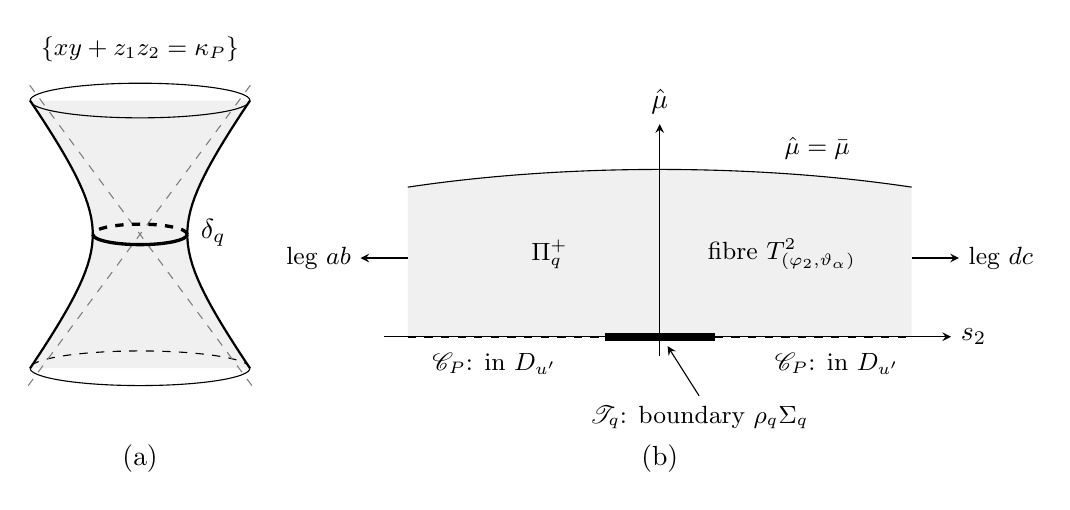
\begin{tikzpicture}[>=stealth]
\begin{scope}
\def\kk{0.6}
\fill[gray!12] plot[domain=-1.7:1.7,samples=40] ({-sqrt(\kk*\kk+0.55*\x*\x)},\x)
  -- plot[domain=1.7:-1.7,samples=40] ({sqrt(\kk*\kk+0.55*\x*\x)},\x) -- cycle;
\draw[thick] plot[domain=-1.7:1.7,samples=40] ({-sqrt(\kk*\kk+0.55*\x*\x)},\x);
\draw[thick] plot[domain=-1.7:1.7,samples=40] ({sqrt(\kk*\kk+0.55*\x*\x)},\x);
\pgfmathsetmacro{\Rr}{sqrt(\kk*\kk+0.55*1.7*1.7)}
\draw (0,1.7) ellipse ({\Rr} and 0.22);
\draw (-\Rr,-1.7) arc (180:360:{\Rr} and 0.22);
\draw[dashed] (\Rr,-1.7) arc (0:180:{\Rr} and 0.22);
\draw[dashed,gray] (-1.42,-1.92) -- (1.42,1.92);
\draw[dashed,gray] (1.42,-1.92) -- (-1.42,1.92);
\draw[very thick] (-\kk,0) arc (180:360:{\kk} and 0.13);
\draw[very thick,dashed] (\kk,0) arc (0:180:{\kk} and 0.13);
\node[right] at (\kk+0.05,0.02) {$\delta_q$};
\node at (0,-2.85) {(a)};
\node[align=center,font=\small] at (0,2.35) {$\{xy+z_1z_2=\kappa_P\}$};
\end{scope}
\begin{scope}[xshift=6.6cm,yshift=-1.3cm]
\fill[gray!12] (-3.2,0) -- (3.2,0) -- (3.2,1.9) .. controls (1.2,2.2) and (-1.2,2.2) .. (-3.2,1.9) -- cycle;
\draw[->] (-3.5,0) -- (3.7,0) node[right] {$s_2$};
\draw[->] (0,-0.25) -- (0,2.7) node[above] {$\hat\mu$};
\draw (3.2,1.9) .. controls (1.2,2.2) and (-1.2,2.2) .. (-3.2,1.9);
\node[font=\small] at (2.0,2.4) {$\hat\mu=\bar\mu$};
\draw[dashed,thick] (-3.2,0) -- (-0.7,0);
\draw[dashed,thick] (0.7,0) -- (3.2,0);
\draw[line width=3pt] (-0.7,0) -- (0.7,0);
\draw[<-] (0.1,-0.12) -- (0.5,-0.75) node[below,font=\small] {$\mathscr T_q$: boundary $\rho_q\Sigma_q$};
\node[below,font=\small] at (-2.1,-0.08) {$\mathscr C_P$: in $D_{u'}$};
\node[below,font=\small] at (2.25,-0.08) {$\mathscr C_P$: in $D_{u'}$};
\draw[->] (-3.2,1.0) -- (-3.8,1.0) node[left,font=\small] {leg $ab$};
\draw[->] (3.2,1.0) -- (3.8,1.0) node[right,font=\small] {leg $dc$};
\node[font=\small] at (-1.4,1.05) {$\Pi^+_q$};
\node[font=\small] at (1.55,1.05) {fibre $T^2_{(\varphi_2,\vartheta_\alpha)}$};
\node at (0,-1.55) {(b)};
\end{scope}
\end{tikzpicture}
\caption{The Morse chart at a node. (a) Schematic real picture of $W^*\cap\mathbb D_P=\{xy+z_1z_2=\kappa_P\}$, two
dimensions lower: in coordinates $\zeta$ with $xy+z_1z_2=\sum_i\zeta_i^2$, the vanishing sphere $\delta_q$ is the waist
$\{\zeta\in\kappa_P^{1/2}\R^4:\sum_i\zeta_i^2=\kappa_P\}$; the dashed lines are the cone of the singular fibre $\kappa_P=0$. (b) The node piece
$\Pi_q^+$ of the $b-a$ passage over the standard half $\{s_1=0,\ \hat\mu\ge0\}$, drawn in the coordinates
$(s_2,\hat\mu)$. Over the interior the fibre is a two-torus (the angle $\varphi_2$ of $\tilde\chi_2$ and the angle
$\vartheta_\alpha$ of $S^1_\alpha$). Over $\hat\mu=0$ the circles $S^1_\alpha$ collapse along $\mathscr C_P$ (dashed), where
$\Pi_q^+$ lies in the divisor $D_{u'}$ and has no boundary; over the thimble $\mathscr T_q$ (thick) they do not, and the
boundary there is the three-sphere $\Sigma_q$, isotopic to $\delta_q$, with multiplicity $\rho_q$
(Lemma~\ref{lem:SI}).}\label{fig:morse}
\end{figure}

\begin{remark}[the sign of $\kappa_P$]\label{rem:kappa}
The window allows both signs of $\eta_P$, hence of $\kappa_P$, and the proof above covers every argument $\phi$ of
$\kappa_P$. The convention of Definition~\ref{def:orient} is also compatible with moving $\kappa_P$ around $0$. In the
family $\{xy+z_1z_2=\kappa\}$, $\kappa=|\kappa|e^{i\phi}$, the sphere $\Sigma^1(\kappa)$ is carried along a path of $\kappa$ by
the complex-linear maps $(x,y,z_1,z_2)\mapsto e^{i\phi/2}(x,y,z_1,z_2)$, which preserve the orientation of the projection
to $(x,z_1)$. A full turn of $\kappa$ acts on $H_3$ of the fibre by the Picard--Lefschetz transformation \cite{Lam81},
which fixes $[\delta]$, because $\langle\delta,\delta\rangle=0$ for the skew intersection form on $H_3$ of a
six-manifold. So the orientations of the $\delta_q$ for different coefficient vectors in $U_\C$ agree under transport.
\end{remark}

\begin{lemma}[change of diagonal]\label{lem:diag}
Replace the labelling $abcd$ of $P$ by $bcda$, which chooses the other diagonal, and keep the order of $u,u'$. Then
$o^{\rm ch}_q$ is unchanged, and the orientation of $\delta_q$ given by Definition~\ref{def:orient} is reversed. Since
$\circv_q$, the coordinate $\lambda_q$ of $K$ and $\rho_q$ change sign as well, $\rho_q\,\delta_q$ and the classes
$\sum_q\lambda_q[\delta_q]$, $\lambda\in K$, do not depend on the choice of diagonals.
\end{lemma}

\begin{proof}
Primes denote the objects of the labelling $a'b'c'd'=bcda$. Then $\mu'_P=\mu_P^{-1}$, $\kappa'_P=e^{\eta_P}-1=-\mu_P\kappa_P$,
$\tilde\chi'_1=\mu_P\tilde\chi_2$, $\tilde\chi'_2=\tilde\chi_1^{-1}$ and $w'_{u'}=-b-w_u$, so $Z$ is unchanged and $Z'$ becomes
$Z'\chi_1^{-1}$; the reference monomial is $b$, so $f'^{(s)}=f^{(s)}/\tilde\chi_1$.

\emph{The chart sign.} Since $\operatorname{val}_c=\operatorname{val}_a+y_1+y_2$, we get $y'_1=y_2$ and $y'_2=-y_1$, and
$\alpha'_q=\alpha_q+\langle\,\cdot\,,b-a\rangle$, which is $\alpha_q+y_1$ up to a constant. The linear map
$(y_1,y_2,\alpha_q)\mapsto(y_2,-y_1,\alpha_q+y_1)$ has determinant $1$, so $o^{\rm ch}_q$ is unchanged.

\emph{The coordinates.} From Definition~\ref{def:morsecoords} and $x'y'+z'_1z'_2-\kappa'_P=f'^{(0)}=f^{(0)}/\tilde\chi_1$ on
$\mathbb D_P$,
\[
x'=y+\mu_P^{1/2}-\mu_P^{-1/2},\qquad y'=\frac{\mu_Px}{\mu_P^{1/2}x-1},\qquad z'_1=c_Zz_1,\qquad z'_2=\frac{z_2}{c_Z\tilde\chi_1},
\]
with a constant $c_Z>0$, the ratio of the two normalisations of $Z$.

\emph{The convention on the thimble.} For $f=xy+z_1z_2-\kappa$ the sphere $\Sigma^1$ bounds the real four-disc
$\{y=e^{i\phi}\bar x,\ z_2=e^{i\phi}\bar z_1,\ |x|^2+|z_1|^2\le|\kappa|\}$, the thimble, which the projection to $(x,z_1)$ maps
onto the ball. So Definition~\ref{def:orient} orients $\delta_q$ as the boundary of the thimble, oriented by $o^{\rm ch}_q$
times the pull-back of the complex orientation of $\C^2_{(x,z_1)}$; for a family of Morse points this orientation is
determined by the tangent space of the thimble at the critical point.

\emph{A deformation.} On $W^*\cap\mathbb D_P$ we have $f^{(0)}=xy+z_1z_2-\kappa_P$. Put $\upsilon:=(1-\mu_P^{1/2}x)^{-1}$, so
that $f'^{(0)}=-\mu_P\,\upsilon f^{(0)}$; on $\mathbb D_P$, $|\mu_P^{1/2}x|\le1/2$, so $\upsilon$ takes values in the disc of
radius $1$ about $1$ without $0$ and has a principal power $\upsilon^s$. For $s\in[0,1]$ the function
$h_s:=\upsilon^sf^{(0)}$ has zero set $W^*\cap\mathbb D_P$. Its critical points satisfy $x=z_1=z_2=0$ (from the derivatives in
$y,z_2,z_1$, since $\upsilon\ne0$) and then $y=s\mu_P^{1/2}\kappa_P$: there is exactly one, $q_s$, with value $-\kappa_P$.
Its Hessian is that of $f^{(0)}$ plus $c_s\,dx^2$, $c_s=s(s-1)\mu_P\kappa_P$; since the matrix $\bigl(\begin{smallmatrix}c&1\\
1&0\end{smallmatrix}\bigr)$ is invertible for every $c$, $q_s$ is nondegenerate. The tangent space of its thimble for the
straight path from $-\kappa_P$ to $0$ is
\[
T_s=\bigl\{v:\ v_y=e^{i\phi}\bar v_x-\tfrac{c_s}2v_x,\ v_{z_2}=e^{i\phi}\bar v_{z_1}\bigr\},
\]
on which the Hessian form is $2e^{i\phi}(|v_x|^2+|v_{z_1}|^2)$; it is a graph over the $(x,z_1)$-plane for every $s$. So the
vanishing spheres of $q_s$ form a continuous family in $W^*\cap\mathbb D_P$, and orienting each as the boundary of its
thimble with the orientation pulled back from $\C^2_{(x,z_1)}$ is continuous in $s$. At $s=0$ this is the orientation of
Definition~\ref{def:orient} for $abcd$ (up to the common factor $o^{\rm ch}_q$). At $s=1$, $h_1=-\mu_P^{-1}f'^{(0)}$ has the
same level sets as $f'^{(0)}$ along the straight paths, so its vanishing sphere is, up to isotopy, the one of the
labelling $bcda$, whose convention pulls back the orientation of $\C^2_{(x',z'_1)}$. The sphere of that convention is
linear in the primed coordinates, and the tangent plane $T'$ of its thimble at $q_1$ need not be $T_1$. At $q_1$, where
$c_1=0$, $\operatorname{Hess}f'^{(0)}=-\mu_P\operatorname{Hess}h_1=-\mu_P\operatorname{Hess}f^{(0)}$, and the path of
$f'^{(0)}$ runs from its critical value $-\kappa'_P$ towards $0$, in the direction of $\kappa'_P=-\mu_P\kappa_P$; so
$\bar\kappa'_P\operatorname{Hess}f'^{(0)}=|\mu_P|^2\,\bar\kappa_P\operatorname{Hess}f^{(0)}$.
Hence $T_1$ and $T'$ are both real four-planes on which $e^{-i\phi}\operatorname{Hess}f^{(0)}$ is real and positive
definite; in particular both are maximal positive planes of the real quadratic form
$\operatorname{Re}(e^{-i\phi}\operatorname{Hess}f^{(0)})$ at $q_1$. After a complex-linear change of coordinates in which
$e^{-i\phi}\operatorname{Hess}f^{(0)}$ becomes $\sum_i\zeta_i^2$, the planes of this kind are the images of $\R^4$ under
$O(4,\C)$, so they form a family $O(4,\C)/O(4)$, which is connected since $O(4)$ meets both components of $O(4,\C)$; the linear thimbles they contain have their boundary spheres
in one level set of the quadratic part, and these spheres move by isotopy along the family. Both thimbles at $q_1$ are
such linear thimbles in one chart. Let $\mathbf w':=(x',y',z'_1,z'_2)$, $A:=d\mathbf w'(q_1)$ and $\mathbf w:=A^{-1}\mathbf w'$.
Since $\mathbf w'(q_1)=0$ and $Q'\circ A=-\mu_PQ$ for the quadratic parts $Q$, $Q'$ of $h_1$ and $f'^{(0)}$ at $q_1$, we have
$h_1=-\mu_P^{-1}f'^{(0)}=-\mu_P^{-1}(Q'(A\mathbf w)-\kappa'_P)=Q(\mathbf w)-\kappa_P$ on $\mathbb D_P$, so $\mathbf w$ are
holomorphic Morse coordinates of $h_1$ at $q_1$ tangent to the identity. In them the thimble of $q_1$ is the linear thimble
with tangent plane $T_1$, and the thimble of the primed convention is the linear thimble with tangent plane
$T'=A^{-1}T'_{\rm lin}$, where $T'_{\rm lin}$ is its tangent plane in the coordinates $\mathbf w'$. So the orientations of $\delta_q$ induced
from oriented thimbles are carried along this family of planes by continuity. On each of them the projections to $(v_x,v_{z_1})$ and to $(v_{x'},v_{z'_1})$, that is to
$(v_y,v_{z_1})$ up to a complex-linear change, are isomorphisms, because a vector with $v_x=v_{z_1}=0$, or with
$v_y=v_{z_1}=0$, is isotropic. So the sign relating the two pulled-back orientations is constant on the family, and it
suffices to compute it on $T_1$. On $T_1$ (where $c_1=0$) the differential of
$(x,z_1)\mapsto(x',z'_1)$ is $(v_x,v_{z_1})\mapsto(e^{i\phi}\bar v_x,c_Zv_{z_1})$, which reverses orientation. So the two
conventions orient $\delta_q$ oppositely.
\end{proof}

\section{The lift of relative tropical \texorpdfstring{$2$}{2}-cycles}\label{sec:lift}

This section proves Theorem~\ref{thm:lift}. Fix an admissible $\Delta$ with a profile $\sigma$ satisfying~\ref{hyp:P}, the
configuration of Section~\ref{ssec:member}, a triangulation $\mathfrak K$ of $B=B'_\sigma$ in which $\Gamma$ is full, and a
relative tropical $2$-cycle $z\in Z(\mathfrak K)$. We construct an integral $4$-chain on the localized mirror $W^*$ of
Definition~\ref{def:Ws} whose boundary is $\sum_q\rho_q(z)\,\Sigma_q$, where $\Sigma_q\subset W^*$ is a three-sphere
isotopic to the vanishing sphere, and carry it to $Y_t$ by the transport lemma. The construction has four steps.

\begin{enumerate}
\item \emph{Transfer and normal form} (Section~\ref{ssec:lift-model}). The cycle $z$ is carried to the mirror base $B_Y$ by
the dual-pair homeomorphism of Section~\ref{sec:legendre}, and the discriminant of $B_Y$ is moved onto the positions over
which $W^*$ has exact local models (the \emph{model complex}). Near the discriminant the transferred cycle is then
replaced, without changing its boundary network, by a sum of finitely many fixed surfaces with integer coefficients: the
\emph{model germs} at the vertices of the discriminant and along its arcs, taken with the multiplicities read off from
the boundary network, and one transverse disc on each arc, with an arbitrary monodromy-invariant coefficient. What is
left lies at positive distance from the discriminant. This is the normal form of Lemma~\ref{lem:normalform}, applied on
$B_Y$, and it is the only place where $z$ enters: near the discriminant only its boundary network and the coefficients of
the transverse discs remain.
\item \emph{Pieces} (Sections~\ref{ssec:lift-legs}--\ref{ssec:lift-cross}). Each model germ and each transverse disc
has an explicit lift near the discriminant, a four-dimensional \emph{piece} of $W^*$, made of subsets of toric divisors,
of the conifold smoothing at a node, and of torus orbits through the positive real locus. At a node the pieces of the
two passages contain the same sphere $\Sigma_q$, and Lemma~\ref{lem:SI} computes their boundary there.
\item \emph{The regular part} (Sections~\ref{ssec:lift-collar} and~\ref{ssec:lift-regular}). The rest of the normalised
chain is lifted over an abstract $2$-complex $\mathscr S$: the disjoint union of its \emph{summands} (the germs, the
discs, the remainder), glued only along the curves where their boundaries cancel. Over $\mathscr S$ the lift is a
bundle of two-tori with integer multiplicities, completed by $3$-chains in the fibres over the edges where several
summands meet. Summands that meet transversally in $B_Y$ are not identified in $\mathscr S$; their lifts are
separate chains, which add in $W^*$. The map to $W^*$ is built cell by cell in regions of $W^*$ that are aspherical,
with fundamental group the local lattice of the base.
\item \emph{The fibre class} (Proposition~\ref{lem:F}). The boundary of the resulting chain is $\sum_q\rho_q\Sigma_q$ plus
closed $3$-cycles in fibres over finitely many points. Each is a multiple of the class of a fibre three-torus, and
pairing with the positive real locus of $W^*$, which meets a fibre torus once and misses every $\Sigma_q$, shows that
the multiples sum to zero.
\end{enumerate}

So the lift is built summand by summand on an abstract domain; summands are glued only along curves where
their boundaries cancel; its boundary, $\sum_q\rho_q(z)\Sigma_q$, is additive in $z$; and the only global input is
Proposition~\ref{lem:F}. The strict tropical
$2$-cycles of \cite{CBM} are a special case, in which every multiplicity of a model germ is $0$ or $\pm1$
(Section~\ref{ssec:lift-cbm}).

The local terms used below refer to the following geometric objects. On $B_Y$, the images of the negative
vertices of $B'_\sigma$ have positive type; these are the \emph{model vertices}. The images of the positive
vertices are the \emph{turning points} (Proposition~\ref{prop:dict}).
\begin{center}\small
\begin{tabular}{p{3.4cm}p{10.8cm}}
term & meaning in the construction\\\hline
model complex & the mirror base with the discriminant moved to the positions of the exact local equations\\
model germ & one of the fixed local surfaces used in the normal form near a discriminant vertex or arc\\
summand & a germ, transverse disc or part of the remainder, with its integral coefficient\\
depth & the nonnegative transverse coordinate measuring distance from the discriminant within a summand\\
inner boundary & the frontier where a local piece joins the lift over the regular part\\
collar & the family of paths, together with its torus orbits, joining these two parts\\
region & an open subset of the localized mirror homotopy equivalent to the torus of the local lattice\\
fibre complex & the cell complex of tori and filling chains used over a simplex of the abstract domain
\end{tabular}
\end{center}

Throughout the section $c$ is a real coefficient vector with $c_0>0>c_n$ for $n\ne0$, in the window of
Definition~\ref{def:window}, with $r\le r_1$ and $\eta_0\le r^2/20$, and $t<t_0(r,\eta_0,\mathscr C_0)$; these are the
members of Theorem~\ref{thm:main} (Section~\ref{ssec:member}). We use the notation of Section~\ref{sec:regime}: $L=\log(1/t)$, the valuations
$\operatorname{val}_n$, the deficits, the weights $\psi_n$, the cut-off constants $\theta_0,\dots,\theta_3$ and $D$,
the constants $e_{\max}$ and $c_M$, the node data of Definition~\ref{def:node}, and the identification of $B_Y$ with the
union of the bounded cells of the tropical hypersurface $\operatorname{Trop}\subset M_\R$. The lattices $\Lambda_Y$,
$\Lambda^M$ are lattices of integral tangent vectors of $B_Y$, contained in $M$; relative cycles on $B_Y$ have
coefficients in the dual local system, the covectors, whose values on $\operatorname{int}F^*_n$ are the classes in
$N/\Z n$ of the elements of $N$.

\subsection{The model complex, the transferred cycle and its normal form}\label{ssec:lift-model}

We first move the discriminant to the positions of the exact local models and transfer the cycle to the mirror base.
The normal-form lemma then separates its boundary germs, transverse discs and a remainder disjoint from the discriminant.

\subsubsection*{The faces \texorpdfstring{$E_e$}{Ee} and the model positions}
The local models of $W^*$ sit over definite points of $B_Y$: the Morse chart over the midpoint of the edge $J_P$ of
Lemma~\ref{lem:gaps}, the models at the vertices of positive type over the segments $J^\flat_\omega$ of
Lemma~\ref{lem:windows}(3), and the leg models over the interior polygons $\Omega_e$ of Definition~\ref{def:legcell}. In general the discriminant $\Gamma_Y$
does not pass through these positions (Remark~\ref{rem:literalpos}). We move it there by a homeomorphism of $B_Y$ that
preserves the dual-pair complex of Proposition~\ref{prop:L1}; Section~\ref{sec:legendre} uses only the combinatorics of
the cells of that complex, not their positions inside the faces of $B_Y$.

We use the faces $E_e$, the interior polygons $\Omega_e$ and the turning points of Definition~\ref{def:legcell} and the
paragraph after it.

For every edge $[u,u']$ of $\mathcal T$ in the dual edge $G^\circ$ of a two-face $G$, or in a two-face $E^\vee$ of
$\Delta^\circ$ dual to an edge $E$ of $\Delta$, we take the vector $w_u\in N$ of Section~\ref{ssec:member}, with
$\langle u,w_u\rangle=1$ and $\langle u',w_u\rangle=0$, put $w_{u'}:=-n_0-w_u$ for a lattice point $n_0$ of the face
$[u,u']^\vee$ of $\Delta$, and write $\alpha_{uu'}:=\langle\,\cdot\,,w_u-w_{u'}\rangle$; at a node these are the vectors
of~\eqref{eq:nodeexp}, with $n_0=a$. At the tropical position of a point of the torus,
$L\alpha_{uu'}=\log|Z|-\log|Z'|$ for the characters $Z=\chi^{w_u}$, $Z'=\chi^{w_{u'}}$, which are the Cox coordinates of
$u$ and $u'$ times units on the chart $U_{u,u'}$. Since $\langle u'-u,w_u-w_{u'}\rangle=-2$, on every polygon $E_e$ with
$e\subseteq[u,u']^\vee$ the level lines of $\alpha_{uu'}$ are parallel lines transverse to $u'-u$, and the edges
$J_\omega$ of $E_e$ for the two-cells $\omega\supset e$ with $\omega^\vee\ni u,u'$ are parallel to $u'-u$.

\begin{definition}[model positions]\label{def:modelpos}
\begin{enumerate}
\item The \emph{model node} of a node parallelogram $P$ is the midpoint $m_P$ of $J_P$. For a unimodular triangle $\omega$
of $\mathcal F_C$ in a two-face $G$, let $u_0,\dots,u_k$ be the lattice points of $G^\circ$ in order, and let $J^\flat_\omega\subseteq J_\omega$
be the segment of Lemma~\ref{lem:windows}(3), which contains the points $p_\omega+s(u_k-u_0)$ with $|s-s_{\rm mid}|\le
1/(4e_{\max})$. The \emph{model vertices} of $\omega$ are points
$m_{\omega,1},\dots,m_{\omega,k}$ of $J^\flat_\omega$ at mutual distances at least $4\theta_3$, in the order in which the
zero-cells $C_Y([u_{i-1},u_i],\omega)$ lie on $J_\omega$. They exist, since that segment has length at least
$k\,c_M/(2e_{\max})\ge4(k-1)\theta_3$.
\item Let $e$ be an edge of $\mathcal F_C$ in the two-skeleton with $\dim e^\vee\ge1$, $\omega\supset e$ a two-cell of a
two-face $G$, and $m$ a model node or vertex of $\omega$, with edge $[u,u']$ of $\mathcal T$. A \emph{leaf path} from $m$
is a path in $E_e$ made of two segments $[m,m']$ and $[m',p_e]$, where $[m,m']$ lies on the level line of $\alpha_{uu'}$
through $m$ and has positive length at most $\theta_3$, and $p_e\in\Omega_e$. Since $\theta_3\le\theta_2/4$, it is a path
of Lemma~\ref{lem:windows}(1$'$). Let $\theta_4\in(0,\theta_2/2]$ be a constant, depending only on the
configuration and the leaf paths, such that at every model node and vertex the points of the leaf paths whose torus
coordinates are within $2\theta_4$ of those of $m$ lie on the first segments.
\item A \emph{model arc system} of $e$ is a family of piecewise linear arcs in $E_e$, each meeting every line parallel to
the direction $u'-u$ of its edge $[u,u']$ of $\mathcal T$ at most once, as follows. If $e$ lies in the interior of a
two-face $G$ with $k$ edges of $\mathcal T$ in $G^\circ$, it consists of $k$ disjoint arcs; the $i$-th joins the $i$-th
model points on the two edges $J_{\omega_\pm}$ of $E_e$, where $\omega_\pm$ are the two two-cells of $G$ containing $e$,
and consists of a leaf path from each of them and an arc in $\Omega_e$. If $e$ lies on an edge $E$ of $\Delta$, it is a
plane graph properly embedded in $E_e$, isomorphic, as a plane graph with its leaves on $\partial E_e$ in their cyclic
order, to $\Gamma_Y\cap E_e$, the graph dual to the triangulation of $E^\vee$ by $\mathcal T$ together with one leaf for
each edge of $\mathcal T$ on $\partial E^\vee$ (Proposition~\ref{prop:L2}(2)); its leaves are the model points on the
edges $J_\omega$ of $E_e$, its leaf edges begin with leaf paths, and its interior vertices and the remaining parts of
its edges lie in $\Omega_e$, each edge dual to $[u_i,u_j]$ being transverse to $u_j-u_i$.
\end{enumerate}
\end{definition}

In~(3) the graph is a tree exactly when $E^\vee$ has no lattice point in its interior; this fails on each of the
examples $X_9$, $X_{19}$ and $X_{20}$ of Section~\ref{sec:examples}. When $e$ lies in the interior of a two-face and both two-cells
$\omega_\pm$ are node parallelograms, the arc joins two model nodes. This occurs at a pentagon (the edge from the centre
shared by its two parallelograms) and at a hexagon on the $A_2$ branch, where the three rhombi share pairwise the edges
$[o,w_{j_0}]$, $[o,w_{j_0+2}]$, $[o,w_{j_0+4}]$ and the three arcs between their model nodes form a cycle of $\Gamma^M$
without vertices of valency three. Nothing below distinguishes these arcs from others.

\subsubsection*{Model arc systems}
We construct model arc systems as homothetic copies of $\Gamma_Y\cap E_e$, joined to the model points by leaf paths. The
arcs, vertices and leaves of $\Gamma_Y\cap E_e$ itself, in their actual positions, are called \emph{original}. Fix $e$ as
in Definition~\ref{def:modelpos}(3). In the picture of $\operatorname{Trop}$ the face $E_e$ is
$-(e^\vee+\nabla^{H'}_e)$, where $e^\vee+\nabla^{H'}_e$ is the face $F^*_e$ of $\partial\nabla^H$ and $\nabla^{H'}_e$ is a
polygon parallel to $e^\vee$. By Lemma~\ref{lem:cayley}(2) for $B_Y$, the cells of $\mathscr P_Y$ in $E_e$ are the sets
$-(F_1(\zeta)+F_2(\zeta))$, $\zeta\in N_\R$, where $F_1(\zeta)$ is the cell of $\mathcal T$ in $e^\vee$ on which
$a\mapsto\langle a,\zeta\rangle+\check h(a)$ is minimal and $F_2(\zeta)$ is the face of $\nabla^{H'}_e$ on which $\zeta$
is minimal; $F_1(\zeta)$ is the lower support of the cell, and only the class of $\zeta$ modulo $\R n+\R n'$ matters. For
a cell $\mathfrak c$ we write $b_{\mathfrak c}$ for the average of its vertices, the vertex of the barycentric subdivision.

\begin{lemma}[original arcs]\label{lem:litarcs}
Let $\tau=[u_i,u_j]$ be an edge of $\mathcal T$ in $e^\vee$, and let $y\in N_\R$ satisfy $\langle u_j-u_i,y\rangle=0$ and
$y\notin\R n+\R n'$. Then the closure of the arc $C_Y(\tau,e)$ is a polygonal arc along which $\langle\,\cdot\,,y\rangle$
is strictly monotone. In particular it meets every line parallel to $u_j-u_i$ at most once.
\end{lemma}

The proof is in Appendix~\ref{app:liftproofs}.

\emph{The construction.} Fix $o_e\in\Omega_e$ and $\mathfrak t_e\in(0,1/2]$ with $\mathfrak k_e(E_e)\subset\Omega_e$ for the
homothety $\mathfrak k_e(p):=o_e+\mathfrak t_e(p-o_e)$. For an edge $J$ of $E_e$ let $y_J$ be the affine function on the
plane of $E_e$ with $y_J=0$ on $J$ and $y_J(o_e)=1$, so that $y_J\ge0$ on $E_e$ and $y_J\circ\mathfrak
k_e=1-\mathfrak t_e+\mathfrak t_ey_J$. Let $S_J:=\{o_e+t(b-o_e):b\in\operatorname{ri}J,\ t>0\}$, an open convex sector; the sectors
of distinct edges are disjoint. A model point $m$ on $J=J_\omega$, with edge $[u,u']$ of $\mathcal T$, lies in
$\operatorname{ri}J\subset S_J$, and the level line of $\alpha_{uu'}$ through $m$ is transverse to $J$. Choose
$\eta_J\in(0,1/4]$ so small that for every model point $m$ on $J$ the point $m'$ of that level line with $y_J(m')=\eta_J$
satisfies $|m'-m|\le\theta_3$ and $m'\in S_J$. The \emph{leaf path} of $m$ in $E_e$ is $[m,m']\cup[m',\mathfrak
k_e(\bar m)]$, where $\bar m$ is the original leaf $C_Y([u,u'],\omega)$ corresponding to $m$ (the $i$-th model point to
the $i$-th original leaf). It is a leaf path in the sense of Definition~\ref{def:modelpos}(2), since
$\mathfrak k_e(\bar m)\in\Omega_e$.

\begin{lemma}[leaf paths]\label{lem:leafpaths}
The segments of the leaf paths in $E_e$ are pairwise disjoint, except that the two segments of one path share the
point $m'$. Each leaf path meets $\partial E_e$ only at its model point, and $\mathfrak k_e(E_e)$ only at its end
$\mathfrak k_e(\bar m)$.
\end{lemma}

The proof is in Appendix~\ref{app:liftproofs}.

\begin{lemma}[model arc systems]\label{lem:arcsystems}
For every triangle ${s_\triangle}$ of $\mathcal T$ in $e^\vee$ let $\mathfrak c_{s_\triangle}$ be the polygon of the proof of
Lemma~\ref{lem:litarcs}, let $\mathfrak c$ run over the three edges of $\mathfrak c_{s_\triangle}$ at which the closed arcs
$\overline{C_Y(\tau,e)}$, $\tau\subset{s_\triangle}$, end with the segments $[b_{\mathfrak c},b_{\mathfrak c_{s_\triangle}}]$, and let
$v_{s_\triangle}$ be the centroid of the triangle with vertices the three points $b_{\mathfrak c}$. Let $\Gamma'_e$ be
$\Gamma_Y\cap E_e$ with each segment $[b_{\mathfrak c},b_{\mathfrak c_{s_\triangle}}]$ replaced by $[b_{\mathfrak c},v_{s_\triangle}]$,
and $\mathscr G_e$ the union of $\mathfrak k_e(\Gamma'_e)$ and of the leaf paths in $E_e$. Then $\mathscr G_e$ is a model
arc system of $e$, and the correspondence which maps $C_Y({s_\triangle},e)$ to $\mathfrak k_e(v_{s_\triangle})$ and each original leaf
to its model point is an isomorphism of plane graphs from $\Gamma_Y\cap E_e$ onto $\mathscr G_e$, preserving the
rotation at every vertex and the cyclic order of the leaves on $\partial E_e$ (the points $\mathfrak k_e(\bar m)$ being
points of degree two). At every interior vertex $\mathfrak k_e(v_{s_\triangle})$ the three angles between consecutive edges
are less than $\pi$.
\end{lemma}

The proof is in Appendix~\ref{app:liftproofs}.

\subsubsection*{The model complex}

\begin{lemma}[the model complex]\label{lem:modelcx}
Fix model positions and model arc systems. There are a regular cell decomposition $\{C^M({\mathfrak p})\}_{{\mathfrak p}\in\mathrm{DP}}$ of $B_Y$
with face poset $(\mathrm{DP},\preceq)$ and a piecewise linear homeomorphism $\Upsilon^M$ of $B_Y$ such that:
\begin{enumerate}
\item $\Upsilon^M(C_Y({\mathfrak p}))=C^M({\mathfrak p})$ for every dual pair ${\mathfrak p}$; $\Upsilon^M$ maps every face $F^*_\omega$ of $B_Y$ onto
itself, and it is isotopic to the identity through homeomorphisms with this property;
\item the zero-cells $C^M([u,u'],\omega)$, $\omega$ a two-cell of a two-face, are the model nodes and model vertices, the
zero-cells $C^M(\tau,e)$, $\tau$ a triangle of $\mathcal T$, are the interior vertices of the model arc systems, and the
arcs $C^M([u,u'],e)$ are the arcs and edges of the model arc systems;
\item the local system $\Lambda^M:=\Upsilon^M_*\Lambda_Y$ is the constant lattice $n^\perp\cap M$ on $\operatorname{int}F^*_n$
and $M/\Z u$ on $R^M_u:=\bigcup_\omega C^M(u,\omega)$, glued on $R^M_u\cap\operatorname{int}F^*_n=C^M(u,n)$ by the
projection $n^\perp\cap M\to M/\Z u$, as $\Lambda_Y$ is (Proposition~\ref{prop:L3}).
\end{enumerate}
\end{lemma}

The proof is in Appendix~\ref{app:liftproofs}.

We write $\Gamma^M:=\Upsilon^M(\Gamma_Y)$ for the \emph{model discriminant}; its vertices are the model nodes, the model
vertices and the turning points $C^M(\tau,e)$, and we call them the \emph{$\Gamma^M$-vertices}. The model vertices are of
positive type and the turning points of negative type on $B_Y$ (Proposition~\ref{prop:L2}(3)).

\begin{remark}[the original positions]\label{rem:literalpos}
The node $C_Y([u,u'],P)$ of $\Gamma_Y$ is the barycentre of the cell of $\mathscr P_Y$ on $J_P$ with lower support
$[u,u']$. If $\check h(u)\ne\check h(u')$ this cell is a segment of length one at an end of $J_P$, and the node lies at
distance $(\mathfrak g_P-1)/2$ from $m_P$, where the Morse chart of $W^*$ sits. This is why the model complex is
needed.
\end{remark}

\subsubsection*{Charts at the model discriminant}
At a model node $m_P$ we use the tropical chart $T_q=(y_1,y_2,\alpha_q)$ of Lemma~\ref{lem:nodemodel}(4), with
$\alpha_q=\alpha_{uu'}-\alpha_{uu'}(m_P)$. Along the model arcs we use the following charts.

\begin{lemma}[tropical charts along the model arcs]\label{lem:tropcharts}
\begin{enumerate}
\item Let $\omega$ be a two-cell of a two-face $G$, $[u,u']$ an edge of $\mathcal T$ in $G^\circ$ and $m$ its model point on
$J_\omega$. Near $m$, $C^M(u,\omega)$ and $C^M(u',\omega)$ are the parts of $J_\omega$ on which $\alpha_{uu'}$ is smaller,
respectively larger, than at $m$.
\item Let $A$ be an arc of the model arc system of $e=[n,n']$, with edge $[u,u']$ of $\mathcal T$, and let $n_y\in N$
complete $n'-n$ to a basis of the lattice $\{x\in N:\langle u,x\rangle=\langle u',x\rangle=0\}$. Then
$(w_u,w_{u'},n'-n,n_y)$ is a basis of $N$, and the level lines of $y:=\langle\,\cdot\,,n_y\rangle$ in $E_e$ are parallel to
$u'-u$, so $A$ is the graph of a piecewise linear function $\bar\alpha$ over an interval of values of $y$:
$\alpha_{uu'}=\bar\alpha(y)$ on $A$. Put $y_e:=\operatorname{val}_{n'}-\operatorname{val}_n$,
$\alpha_e:=\alpha_{uu'}-\bar\alpha(y)$ and $T_e:=(y_e,\alpha_e,y)$. Near the part of $A$ in the interior of $E_e$, $T_e$
is a piecewise linear homeomorphism onto an open subset of $\R^3$, mapping $\operatorname{int}F^*_n$, $E_e$ and
$\operatorname{int}F^*_{n'}$ into $\{y_e<0\}$, $\{y_e=0\}$ and $\{y_e>0\}$, $A$ onto a segment of the $y$-axis, and the
cells $C^M(u,e)$, $C^M(u',e)$ near $A$ into $\{y_e=0,\ \alpha_e<0\}$ and $\{y_e=0,\ \alpha_e>0\}$.
\end{enumerate}
\end{lemma}

The proof is in Appendix~\ref{app:liftproofs}.

So at every model node and model vertex the side $\alpha_{uu'}>\alpha_{uu'}(m)$ is the side of $u'$, the side of the
tentacles of the divisor $D_{u'}$. The model nodes are the midpoints of pairwise distinct edges $J_P$ of $B_Y$; this
includes the two nodes of a pentagon and the three nodes of an $A_2$ hexagon, which share the edge $[u,u']$ of
$\mathcal T$. We take the $\varrho_q$ of Lemma~\ref{lem:nodemodel}(4) so small that the cubes
$T_q^{-1}([-\varrho_q,\varrho_q]^3)$ are pairwise disjoint and disjoint from fixed neighbourhoods of the other
$\Gamma^M$-vertices.

\begin{lemma}[model cells near the model discriminant]\label{lem:place}
There is $r_S\in(0,\theta_4/4]$, depending only on the configuration, the model positions and $\Upsilon^M$, such that:
\begin{enumerate}
\item at each model node $m_P$, $T_q^{-1}(\{y_1=0,\ \alpha_q\ge0\})\cap T_q^{-1}([-r_S,r_S]^3)$ is the intersection with
that cube of the closure of $C^M(u',ab)\cup C^M(u',P)\cup C^M(u',cd)$, and it is bounded on $\Gamma^M$ by the model arcs of
the legs over $ab$ and $dc$; likewise $\{y_2=0,\ \alpha_q\ge0\}$ with $bc$ and $da$, and $\{\alpha_q\le0\}$ with $u$ in
place of $u'$;
\item near each model vertex $m=m_{\omega,i}$, $\omega=[n_a,n_b,n_c]$, with edge $[u,u']=[u_{i-1},u_i]$ of $\mathcal T$ and
edges $e_1,e_2,e_3$ of $\omega$, the closure of $C^M(u',\omega)\cup\bigcup_kC^M(u',e_k)$ is the union of three closed
sectors, one in each $E_{e_k}$, meeting along the half-edge $C^M(u',\omega)$ of $J_\omega$, the $k$-th bounded by that
half-edge and the model arc $C^M([u,u'],e_k)$; likewise with $u$;
\item near each turning point $C^M(\tau,e)$, $\tau=[u_1,u_2,u_3]$, the closure of $C^M(u_i,e)$ is the sector of $E_e$ between
the model arcs of $[u_i,u_j]$ and $[u_i,u_k]$, of angle less than $\pi$;
\item near each model arc $A$ in the interior of $E_e$, in the chart $T_e$, the closures of $C^M(u',e)$ and $C^M(u,e)$ are
$\{y_e=0,\ \alpha_e\ge0\}$ and $\{y_e=0,\ \alpha_e\le0\}$.
\end{enumerate}
\end{lemma}

The proof is in Appendix~\ref{app:liftproofs}.

\subsubsection*{The transferred cycle}
We apply Definition~\ref{def:transfer} with $\Upsilon=\Upsilon^M$: $\mathfrak h=\Upsilon^M\circ\mathcal L\circ g_C\colon B'_\sigma\to
B_Y$, $\kappa_{\mathfrak h}\colon\Lambda\to\mathfrak h^*(\Lambda^M)^\vee$, the coefficient groups $F^*(s)$ and $\mathcal D^*(E)=\Z d^*_A$,
$d^*_A=\langle\,\cdot\,,n'-n\rangle$ on the arc $A$ of $([u,u'],[n,n'])$. For $z\in Z(\mathfrak K)$ the \emph{transferred
cycle} is
\[
z^M:=\mathfrak h_*z\in Z\bigl(\mathfrak h(\mathfrak K_1);F^*,\mathcal D^*\bigr),
\]
a relative cycle on the triangulation $\mathfrak h(\mathfrak K_1)$ of $B_Y$, in which $\Gamma^M$ is full. By
Proposition~\ref{prop:transfer} its boundary network $b^M:=\partial z^M$ has the integers of $\partial z$, and
$\rho^*(z^M)=\rho(z)$; we write $\rho$ for $\rho^*$ and $\mathrm{Bal}(\Gamma^M)$ for the group of balanced networks on
$\Gamma^M$, the $1$-cycles of $C_*(\Gamma^M;\mathcal D^*)$. By Proposition~\ref{prop:dict}(2),(3) the stalks
$\operatorname{Inv}^*$ are: on an arc, $\{v:v(u'-u)=0\}$, of rank two, with basis $d^*_A$ and $g^*_A:=\langle\,\cdot\,,n_y
\rangle$ (Lemma~\ref{lem:crossing}); at a model node, the same group, with basis $\langle\,\cdot\,,b-a\rangle$,
$\langle\,\cdot\,,c-b\rangle$; at a model vertex, of positive type, a group of rank two containing the covectors $d^*_A$ of
its three arcs; at a turning point $C^M(\tau,e)$, of negative type, $\Z d^*_e$, $d^*_e:=\langle\,\cdot\,,n'-n\rangle$ for
$e=[n,n']$, the common covector of its three arcs up to sign.

Lemmas~\ref{lem:nbhd} and~\ref{lem:normalform} hold on $B_Y$, for $\Gamma^M$ and the coefficients $F^*$, $\mathcal D^*$,
on every triangulation in which $\Gamma^M$ is full: their proofs use only a triangulated three-manifold, a full graph and
the flat sections of a local system (Remark~\ref{rem:nbhdscope}). Equivalently, for a triangulation $\mathfrak K^*$ of $B_Y$
refining $\mathfrak h(\mathfrak K_1)$ the map $\mathfrak h^{-1}$ is linear on the simplices of $\mathfrak K^*$, and Lemma~\ref{lem:transport}
applied to $(\mathfrak h^{-1},\kappa_{\mathfrak h}^{-1})$ identifies the chain complexes, coefficient systems and stalks on $\mathfrak K^*$ with those
on the triangulation $\mathfrak h^{-1}(\mathfrak K^*)$ of $B'_\sigma$, in which $\Gamma$ is full.

\begin{lemma}[balanced leg data]\label{lem:unitgerms}
At a $\Gamma^M$-vertex $p$ let $\mathrm{Bal}_p$ be the lattice of \emph{balanced leg data}: the vectors $(c_A)$ of coefficients on
the arcs $A$ at $p$, oriented away from $p$, with $\sum_Ac_Ad^*_A=0$ in $\operatorname{Inv}^*(p)$. Then: at a model vertex,
with the $d^*_A$ oriented so that $d^*_1+d^*_2+d^*_3=0$, $\mathrm{Bal}_p=\Z(1,1,1)$; at a turning point, with the $d^*_A$ oriented
equal, $\mathrm{Bal}_p=\{c_{12}+c_{13}+c_{23}=0\}$; at a model node, with $d^*_{ab}=d^*_{dc}=\langle\,\cdot\,,b-a\rangle$ and
$d^*_{bc}=d^*_{da}=\langle\,\cdot\,,c-b\rangle$, $\mathrm{Bal}_p=\{c_{ab}=-c_{dc},\ c_{bc}=-c_{da}\}$. A balanced network
restricts at $p$ to an element of $\mathrm{Bal}_p$.
\end{lemma}

\begin{proof}
At a model vertex the three $d^*_A$ are $\pm\langle\,\cdot\,,e_k\rangle$ for the three edges $e_k$ of a unimodular triangle,
which span a lattice of rank two and satisfy one relation; at a turning point they are equal up to sign; at a node
$\langle\,\cdot\,,b-a\rangle$ and $\langle\,\cdot\,,c-b\rangle$ are independent. The last statement is the balance of a balanced network
at $p$, a relation in $F^*(p)=\operatorname{Inv}^*(p)$. This is Lemma~\ref{lem:legdata}, transported by $\mathfrak h$ and
$\kappa_{\mathfrak h}$, with the
vertex types exchanged.
\end{proof}

\subsubsection*{Model germs}
All germs below are fixed once, after the configuration, the model positions and $\Upsilon^M$, and before $z$ and $t$.
They lie in $N_0$, the $r_0$-neighbourhood of $\Gamma^M$, where $r_0\le r_S/4$ is so small that $N_0$ lies in the union of
the cubes $T_q^{-1}([-r_S,r_S]^3)$, the neighbourhoods of the model vertices and turning points of
Lemma~\ref{lem:place}(2),(3), and the domains of the charts $T_e$. Each germ is a piecewise linear surface with boundary
on $\Gamma^M\cup\partial N_0$, carrying a coefficient that is a flat section of $(\Lambda^M)^\vee$ over it. The
\emph{away-oriented leg data} of a germ at a $\Gamma^M$-vertex $p$ are the coefficients $c_A$ of its boundary
$\sum_Ac_Ad^*_A[A]$ on the arcs $A$ at $p$, each oriented away from $p$.

\begin{enumerate}
\item[(M1)] \emph{Node halves.} At a model node $m_P$ the four \emph{standard halves} are
$T_q^{-1}(\{y_1=0,\ \pm\alpha_q\ge0\})$ (the \emph{$b-a$ passage}, along the legs over $ab$ and $dc$) and
$T_q^{-1}(\{y_2=0,\ \pm\alpha_q\ge0\})$ (the \emph{$c-b$ passage}, along $bc$ and $da$). We use the side $\alpha_q\ge0$.
The \emph{unit germ} $g_{ab}$ is the $b-a$ half with the orientation of the frame $(y_2,\alpha_q)$ and the covector
$-\langle\,\cdot\,,b-a\rangle$; the unit germ $g_{bc}$ is the $c-b$ half with the orientation of the frame
$(y_1,\alpha_q)$ and the covector $+\langle\,\cdot\,,c-b\rangle$. The boundary of $g_{ab}$ runs from the leg over $ab$ to the leg over $dc$, and that of
$g_{bc}$ from the leg over $da$ to the leg over $bc$; so their away-oriented leg data are $(c_{ab},c_{bc})=(1,0)$ and
$(0,1)$, and $\rho_q(g_{ab})=1$, $\rho_q(g_{bc})=-1$. Both covectors lie in $\operatorname{Inv}^*(m_P)$.
\item[(M2)] \emph{Tripods.} At a model vertex $m=m_{\omega,i}$ the unit germ is the union of the three sectors of
Lemma~\ref{lem:place}(2) on the side of $u'$. Orient the edges $e_k$ of $\omega$ cyclically, so that $e_1+e_2+e_3=0$, orient
the sector in $E_{e_k}$ so that its boundary leaves $m$ along its model arc (and hence arrives at $m$ along the half-edge
$C^M(u',\omega)$), and give it the covector $\langle\,\cdot\,,e_k\rangle$, which is $d^*_A$ for its arc. The three sectors
induce the same orientation on the half-edge, their covectors sum to zero there, and the away-oriented leg data are
$(1,1,1)$.
\item[(M3)] \emph{Turning germs.} At a turning point $C^M(\tau,e)$, $\tau=[u_1,u_2,u_3]$, $e=[n,n']$, let $A_{ij}$ be the arc
of $[u_i,u_j]$ and $C(u_i)$ the sector of Lemma~\ref{lem:place}(3) between $A_{ij}$ and $A_{ik}$. Fix an orientation $o_e$
of $E_e$. With every sector oriented by $o_e$ and carrying $d^*_e$, the leg data $(c_{12},c_{13},c_{23})$ of the three
sectors sum to zero, and each sector has data $\pm1$ on its two arcs and $0$ on the third. We label $\tau$ so that
$C(u_1)=(1,-1,0)$, $C(u_2)=(-1,0,1)$, $C(u_3)=(0,1,-1)$. The \emph{turning germs} are $\mathrm{Turn}(u_1):=C(u_1)$ and
$\mathrm{Turn}(u_3):=C(u_3)$ with orientation $o_e$ and $\mathrm{Turn}(u_2):=C(u_2)$ with orientation $-o_e$, all with
covector $d^*_e$; their leg data are $(1,-1,0)$, $(1,0,-1)$, $(0,1,-1)$. The chain $\mathrm{Turn}(u_1)-\mathrm{Turn}(u_2)+
\mathrm{Turn}(u_3)$, the full disc of $E_e$ about the vertex with orientation $o_e$, has zero leg data.
\item[(M4)] \emph{Exit sheets and reference sheets.} Orient each arc $A$ from one end $p_0$ to the other end $p_1$ and fix,
in the part of $A$ in $\Omega_e$, five points in this order:
$y^*_{A,0},\ y^0_A,\ \mathfrak x_A,\ y^1_A,\ y^*_{A,1}$, and take $r_0$ at most a quarter of their mutual distances, of
their distances from $A\setminus\Omega_e$ and of their distances from the ends $p_0,p_1$ of $A$, so that the stretches of
length at most $r_0$ about $y^*_{A,p}$ below lie in $\Omega_e$ and away from the balls $B^0_{p_0}$, $B^0_{p_1}$ of
Section~\ref{ssec:lift-collar}, whose radius is at most $r_0$. A unit germ at an end $p$ of $A$ that uses $A$ continues along $A$
as its \emph{exit sheet}: in the chart $T_e$, the half-plane $\{y_e=0,\ \alpha_e\ge0\}$ (the closure of $C^M(u',e)$) or
$\{y_e=0,\ \alpha_e\le0\}$ (that of $C^M(u,e)$), according to its side at $p$, from $p$ to $y^0_A$ if $p=p_0$ and to
$y^1_A$ if $p=p_1$. The \emph{reference side} of every arc is $\alpha_e\ge0$. Fix a convex polygon $\mathsf P\subset\R^2$,
symmetric about $0$, with gauge $\varrho_{\mathsf P}$. An exit sheet on the side $\alpha_e\le0$ is \emph{rotated} to the
reference side at $y^*_{A,p}$: in the chart it is the half-plane $\alpha_e\le0$ up to $y^*_{A,p}$, the normal half-disc
$\{y=y^*_{A,p},\ y_e\ge0,\ \varrho_{\mathsf P}(y_e,\alpha_e)\le r_0\}$ there, and the half-plane $\alpha_e\ge0$ after it.
All half-planes are truncated at $\varrho_{\mathsf P}\le r_0$. The \emph{reference sheet} of $A$ with coefficient
$c_Ad^*_A$ is the half-plane $\alpha_e\ge0$ over $[y^0_A,y^1_A]$, oriented so that its boundary on $A$ runs in the direction
of $A$.
\item[(M5)] \emph{Transverse discs.} At $\mathfrak x_A$, the normal disc $\mathfrak N_A:=\{y=y(\mathfrak x_A),\
y_e^2+\alpha_e^2\le r_0^2\}$ in the chart $T_e$, cooriented by $A$: (orientation of $\mathfrak N_A$, direction of $A$) is
the orientation of $B_Y$.
\end{enumerate}

At an end $p$ of $A$ the exit sheets on a given side come from one germ type: at a turning point the side $u_i$ of the
arc of $[u_i,u_j]$ belongs to $\mathrm{Turn}(u_i)$, and at a model node or vertex each leg is used by one germ type, on
the side $u'$. An arc joining two model nodes receives one exit sheet from each end, cut at $y^0_A$ and $y^1_A$. The rotation through the half-plane $y_e>0$ rather than through $y_e<0$ is a convention; the other choice changes
the chain by a transverse disc with coefficient in $\Z d^*_A$.

By Lemma~\ref{lem:unitgerms} the unit germs at $p$ form a $\Z$-basis of $\mathrm{Bal}_p$: $g_{ab},g_{bc}$ at a model node, the
tripod at a model vertex, $\mathrm{Turn}(u_1),\mathrm{Turn}(u_2)$ at a turning point. For $b\in\mathrm{Bal}(\Gamma^M)$ write
$b_p=\sum_gm_g(b)\,\partial g$ at every $\Gamma^M$-vertex $p$, with integers $m_g(b)$ ($g$ running over the
unit germs of the basis at $p$).

\begin{definition}[the standard chain]\label{def:std}
For $b\in\mathrm{Bal}(\Gamma^M)$ the \emph{standard chain} $\mathrm{Std}^M(b)$ is the sum over all $\Gamma^M$-vertices $p$ of
$\sum_gm_g(b)\,g$, each unit germ with its exit sheets, cut transversally at $y^0_A$ or $y^1_A$, plus, on every arc
$A$, the reference sheet with covector $c_Ad^*_A$ between $y^0_A$ and $y^1_A$, where $c_Ad^*_A[A]$ is the part of $b$
on $A$.
\end{definition}

Along $A$ the exit sheets arriving from each end carry, on the reference side, covectors summing to $c_Ad^*_A$ with the
orientation of the reference sheet, by the balance of $b$ along the arc; so the transverse cut segments cancel, and
$\mathrm{Std}^M(b)$ is a relative cycle of $(N_0,\partial N_0\cup\Gamma^M)$ with boundary network $b$. It is linear in
$b$.

Where sheets of $\mathrm{Std}^M(b)$ coincide as sets, namely sheets on the reference side of one arc, their
coefficients add.

\subsubsection*{The normal form on \texorpdfstring{$B_Y$}{BY}}
Let $z^M=\mathfrak h_*z$ and $b^M=\partial z^M$. Choose a triangulation $\mathfrak K_2^0$ of $B_Y$ refining $\mathfrak h(\mathfrak K_1)$, in which
$\Gamma^M$, the germs (M1)--(M5) and their junction segments are subcomplexes, and which is so fine near $\Gamma^M$ that
the simplicial neighbourhoods below lie in the interior of $N_0$. Let $\mathfrak K_2$ be a derived subdivision of
$\mathfrak K_2^0$, in which $\Gamma^M$ is full and the germs are subcomplexes; choose its derived points off the points
$\mathfrak x_A$, so that $\mathfrak x_A$ lies in the interior of an edge $E_A$ of $\mathfrak K_2$ in $A$; and let
$\mathfrak K_2'$ be a derived subdivision of $\mathfrak K_2$ whose new vertex on $E_A$ is $\mathfrak x_A$. Put
$U:=N(\Gamma^M,\mathfrak K'_2)$, the union of the closed simplices meeting $\Gamma^M$. Then $\operatorname{sd}z^M$ lies on
$\mathfrak K_2'$, and $\mathrm{Std}^M(b^M)\cap U$ is a relative cycle of $(U,\partial U\cup\Gamma^M)$ on $\mathfrak K'_2$ with
boundary network $b^M$: its coefficients lie in the stalks, since near a $\Gamma^M$-vertex only the germs of that vertex
occur and along an arc only covectors in $\operatorname{Inv}^*(A)$; and an edge of $U$ not in $\partial U$ meets
$\Gamma^M$, so that all $2$-simplices at it lie in $U$ and intersecting with $U$ creates boundary only on $\partial U$. By
Lemma~\ref{lem:normalform}, with the edge $E_A$ chosen in each arc $A$,
\begin{equation}\label{eq:nf1}
\operatorname{sd}z^M-\partial w=\mathrm{Std}^M(b^M)\cap U+\sum_Av_A\,\bar D(E_A)+y,\qquad v_A\in\operatorname{Inv}^*(A),
\end{equation}
with $w$ a $3$-chain in $U$, $v_A\bar D(E_A)$ the transverse disc at $E_A$ in $\mathfrak K'_2$ (Definition~\ref{def:transverse}), centred at $\mathfrak x_A$, and $y$
supported in $B_Y\setminus\operatorname{int}U$. Of Lemma~\ref{lem:nbhd} only the surjectivity in part~(1) enters, applied to the chain
$\operatorname{sd}z^M|_U-\mathrm{Std}^M(b^M)\cap U$, which has zero boundary on $\Gamma^M$.

We then make two local replacements. A \emph{local replacement} replaces a chain $C$ by a chain $C'$ with the same
boundary on $\Gamma^M$ and adds a chain $R$ supported off $\Gamma^M$ with $\partial R=\partial C-\partial C'$ off $\Gamma^M$;
it preserves the boundary network.
\begin{itemize}
\item \emph{Straightening the transverse discs.} Let $N_{\varepsilon_A}(\mathfrak x_A)$ be a piecewise linear regular
neighbourhood of $\mathfrak x_A$ of diameter at most $\varepsilon_A$, for instance a closed star in a derived subdivision in
which $\bar D(E_A)$ and $\Gamma^M$ are subcomplexes. By regular-neighbourhood theory \cite[Ch.~3]{RS} the triple
$(N_{\varepsilon_A},N_{\varepsilon_A}\cap\bar D(E_A),N_{\varepsilon_A}\cap\Gamma^M)$ is unknotted (a ball, a proper disc and a
proper arc meeting it once transversally), so $\partial N_{\varepsilon_A}$ minus the two points of $\Gamma^M$ is an open
annulus in which $\partial N_{\varepsilon_A}\cap\bar D(E_A)$ is essential. Let $\mathfrak N_A^{\varepsilon'_A}$ be the normal
disc of (M5) of radius $\varepsilon'_A\le r_0$, so small that its solid cylinder $T_e^{-1}(\{y_e^2+\alpha_e^2\le
\varepsilon'^2_A,\ |y-y(\mathfrak x_A)|\le\varepsilon'_A\})$ lies in $\operatorname{int}N_{\varepsilon_A}$. Replace
$v_A(\bar D(E_A)\cap N_{\varepsilon_A})$ by $v_A\mathfrak N^{\varepsilon'_A}_A$ plus $v_A$ times an embedded annulus in
$N_{\varepsilon_A}\setminus(\Gamma^M\cup\text{cylinder})$ between the two essential circles; $v_A$ extends over it because it
lies in a punctured neighbourhood of an arc point.
\item \emph{Smoothing the rotations.} On a stretch $\mathfrak a_{A,p}\ni y^*_{A,p}$ of length at most $r_0$ replace every
rotated exit sheet by the union of the rays $\{(\varrho\cos\Theta(y),\varrho\sin\Theta(y),y):\varrho\ge0\}$ in the
coordinates $(y_e,\alpha_e,y)$, truncated at $\varrho_{\mathsf P}\le\varrho_0$, with $\Theta$ smooth and monotone,
$\Theta=-\pi/2$ near the start and $\Theta=\pi/2$ near the end of the stretch, passing through $\Theta=0$; add the strip on
the polygonal cylinder $\{\varrho_{\mathsf P}=\varrho_0\}$ over the stretch between the two outer curves, closed up at its
ends.
\end{itemize}
The sizes $\varepsilon_A$ and $\varrho_0$ are chosen so that the neighbourhoods $N_{\varepsilon_A}(\mathfrak x_A)$ and the
solid cylinders $\{\varrho_{\mathsf P}\le\varrho_0\}$ over the stretches lie in $\operatorname{int}U$, and each meets no
summand other than the sheets along its own arc.

\begin{lemma}[normal form of the transferred cycle]\label{lem:nfY}
The result is a relative cycle
\begin{equation}\label{eq:nf2}
z^\natural=\mathrm{Std}^M(b^M)+\sum_Av_A\,\mathfrak N_A+y^\natural,\qquad v_A\in\operatorname{Inv}^*(A),
\end{equation}
with boundary network $b^M$ and $\rho(z^\natural)=\rho(z)$, where $\mathrm{Std}^M(b^M)$ now has smooth rotations and is
truncated at $\partial U$, $\mathfrak N_A$ is $\mathfrak N^{\varepsilon'_A}_A$ continued by the annulus and by $\bar D(E_A)$
outside $N_{\varepsilon_A}(\mathfrak x_A)$, and $y^\natural$ is $y$ plus the strips of the smoothing. Let $r_\natural>0$ be
the distance, in a fixed metric on $B_Y$, from $\Gamma^M$ to the union of $\operatorname{supp}y^\natural$ and of the parts
of the transverse discs outside the normal discs $\mathfrak N^{\varepsilon'_A}_A$. Within distance $r_\natural$ of
$\Gamma^M$, $z^\natural$ is exactly $\mathrm{Std}^M(b^M)+\sum_Av_A\mathfrak N^{\varepsilon'_A}_A$: germs in the positions of
Lemma~\ref{lem:place} and normal discs at the points $\mathfrak x_A$.
\end{lemma}

\begin{proof}
The local replacements preserve the boundary network. The strips of the smoothing lie at distance at least
$\varrho_0/C_{\mathsf P}$ from $\Gamma^M$, $C_{\mathsf P}$ the equivalence constant of $\varrho_{\mathsf P}$ and the
Euclidean norm; the annuli lie in compact subsets of $N_{\varepsilon_A}\setminus\Gamma^M$; $y$ lies off
$\operatorname{int}U$; and the transverse discs meet $\Gamma^M$ only at their centres. So $r_\natural>0$, with
$r_\natural\le\min(\varepsilon'_A,\varrho_0/C_{\mathsf P})$.
\end{proof}

The homology class of $z$ plays no role: what follows needs only a relative cycle with the boundary network of $z$, and
Lemma~\ref{lem:nfY} provides one of the required shape.

\emph{Summands.} Near $\Gamma^M$ the normal form~\eqref{eq:nf2} is a finite sum of surfaces with integer
coefficients: for each $\Gamma^M$-vertex $p$ and each unit germ $g$ at $p$, the surface of $g$ (its component at $p$ in
$N_0$ together with its exit sheets, rotated and smoothed where required, up to $y^0_A$ or $y^1_A$), with coefficient
$m_g(b^M)$ times the covector of $g$; the reference sheets, with coefficients $c_Ad^*_A$; and the transverse discs
$v_A\mathfrak N_A$. Where surfaces of this list coincide as sets, which happens only for sheets on the reference side of
one arc, we add their coefficients. A \emph{summand} is a maximal connected part of one of these surfaces, or of a
union of coincident sheets, on which the total coefficient is constant, except that the three sectors of a tripod, with
their exit strips, form one summand: its half-edge $C^M(u',\omega)$ is an interior branching curve, along which the
three coefficients $m\langle\,\cdot\,,e_k\rangle$ sum to zero with the orientations of (M2). In particular the part of a unit germ at its
vertex and its exit strips, including the start of a rotation, belong to one summand up to the first place where
another sheet joins them: the transverse segments where a germ continues as its own exit strip carry the same
coefficient on both sides and are interior to one summand. Two summands are \emph{adjacent} along a
\emph{junction segment}, a curve other than the half-edge of a tripod across which the total coefficient on one side of
the arc changes. Junction segments occur only where a rotated exit strip reaches a reference side that already carries a
strip (inside the polygonal cylinder at the far end of the stretch; outside it, where the piecewise linear normal
half-disc of the rotation at $y^*_{A,p}$ meets the reference-side strip). Where a rotated strip reaches an empty
reference side, it simply continues there, and where the exit strips on the reference side meet the reference sheet, at
$y^0_A$ and $y^1_A$, they already total $c_Ad^*_A$ with the orientation of the reference sheet (by the balance of $b^M$
along $A$); in both cases the total coefficient does not change and the curve is interior to one summand. Along a
junction segment every
adjacent coefficient is a multiple of $d^*_A$, and the multiples sum to zero with the orientation signs, because
$z^\natural$ is a relative cycle with boundary only on $\Gamma^M$. Inside the stretch, after $y^*_{A,p}$, the reference-side
sheet carries one coefficient inside the cylinder $\{\varrho_{\mathsf P}<\varrho_0\}$, where the smoothed strip is still
rotating, and another outside it, where the piecewise linear rotated sheet has already arrived; they meet the correction
strip of the smoothing along the seam $\{\varrho_{\mathsf P}=\varrho_0\}$, at distance at least $\varrho_0/C_{\mathsf P}\ge
r_\natural$ from $\Gamma^M$. Summands may also meet transversally (a transverse disc and a sheet; the two node halves
along $C^M(u',P)$; exit sheets of different germs meeting only on $\Gamma^M$); such meetings are not junctions.

\subsection{Pieces along legs, at vertices and at turning points}\label{ssec:lift-legs}

We lift the boundary germs in the binomial and pair-of-pants models of the localized hypersurface.
The positive real section fixes compatible base points for the torus orbits, and Lemma~\ref{lem:windows} places these orbits in regions where the equations are exact.

\subsubsection*{The positive section}
\begin{lemma}[the positive locus]\label{lem:possec}
For $t$ small and every real $c$ with the sign pattern:
\begin{enumerate}
\item the positive real locus $\Sigma^+:=Y_t\cap(\R_{>0})^4$ is a smooth strictly convex three-sphere in the torus
(compare \cite[\S3.1]{AGIS20});
\item for $s\in[0,1]$ the positive locus $\Sigma^+_s$ of $W_s$ is a smooth closed three-manifold, the $\Sigma^+_s$ form a
smooth family, and $\operatorname{Log}(\Sigma^+_0)/L$ is a star-shaped sphere within $O(1/L)$ of $B_Y$. Radial projection
therefore defines a section $\mathfrak s^\vee\colon B_Y\to\Sigma^+_W:=\Sigma^+_0\subset W^*$.
\end{enumerate}
\end{lemma}

\begin{proof}
(1) On the positive part of the torus, $F_t/(\gamma_0x^0)=1-\sum_{n\ne0}|\gamma_n/\gamma_0|e^{\langle w,n\rangle}$ with
$w=\operatorname{Log}x$. The sum is strictly convex in $w$, because the $n\ne0$ span $N_\R$, and proper, because $0$ is
interior to their convex hull; its value at $w=0$ is $O(t^{k_0+\min h_C})<1$. So $\{\sum=1\}$ is a smooth strictly convex
sphere.

(2) Complex conjugation preserves $F^{(s)}$, since the coefficients are real and the weights depend only on moduli; so
at a real point $dF^{(s)}$ maps real tangent vectors to $\R$ and imaginary ones to $i\R$, and real rank two
(Lemma~\ref{lem:W}(1)) forces $dF^{(s)}|_{\R^4}\ne0$. Hence $\Sigma^+_s$ is a regular level set, and the family is smooth.
It does not meet the toric boundary: on the nonnegative part of a divisor the origin monomial vanishes and the others are
nonpositive, the maximal one having weight one. Along a ray $w=\lambda w_0$, at a zero of $F^{(0)}$ the origin monomial
lies between $\mathfrak m$ and $|\mathcal A|\mathfrak m$, $\mathfrak m$ the largest monomial; so the deficit of the origin is
$O(1/L)$, $w/L$ lies within $O(1/L)$ of $B_Y$, and $|w|=O(L)$. A monomial $n\ne0$ of positive weight has
$d_n\le\tilde d_n<\theta_1/2\le1/2$, so $|\gamma_nx^n|\ge t^{1/2}\mathfrak m$, that is $\langle w,n\rangle\ge
L(H(n)-\tfrac12)-O(1)\ge\tfrac L2-O(1)$, since $H(n)\ge1$ by~\eqref{eq:lambdagap}. The function
$\mathfrak S(\lambda):=\sum_{n\ne0}\psi_n|\gamma_n/\gamma_0|e^{\langle w,n\rangle}$ equals $1$ at a crossing; with the weights
held constant its derivative with respect to $\log\lambda$ is at least $L/2-O(1)$ there, and the derivatives of the weights
are $O(1)$ (Lemma~\ref{lem:refined}(2)) and multiply monomials in transition, of total size $O(t^{\theta_1/4})$ relative to
the origin. So each ray crosses $\Sigma^+_0$ exactly once, transversally.
\end{proof}

For a primitive covector $v$ in the stalk of $(\Lambda^M)^\vee$ at a point of $B_Y\setminus\Gamma^M$, the quotient of the
fibre torus $\Lambda^M\otimes U(1)$ by $\mathbb T(v):=\ker v\otimes U(1)$ is the circle of the character $\chi^{\tilde v}$
for any lift $\tilde v\in N$ of $v$, and its phase is $0$ on $\Sigma^+_W$. So the union of the $\mathbb T(v)$-orbits
through the points of $\mathfrak s^\vee$ over a surface with coefficient $v$ is contained in $\{\arg\chi^{\tilde v}=0\}$.

\subsubsection*{Where the localized mirror is given by exact models}
We use Lemma~\ref{lem:windows}: on the sets listed there the weights of the localized mirror are exactly $0$ or $1$. For
node parallelograms, item (1$'$) covers the stretches of the model arcs from a model node to $\Omega_e$, along the leaf
paths, and for triangles those from a model vertex.

\subsubsection*{Normalised coordinates along the model arcs}
Let $A$ be an arc of the model arc system of $e=[n,n']$, with edge $[u,u']$ of $\mathcal T$ and $n_y$ as in
Lemma~\ref{lem:tropcharts}(2). On the chart $U_{u,u'}$ we use $Z=\chi^{w_u}$, $Z'=\chi^{w_{u'}}$, $\chi_1=\chi^{n'-n}$ and
$\chi_2=\chi^{n_y}$. The \emph{normalised coordinates} along $A$ are $\hat Z=Z/\nu_Z$ and $\hat Z'=Z'/\nu_{Z'}$, where
$\nu_Z,\nu_{Z'}>0$ are smooth functions of $\log|\chi_1|$ and $\log|\chi_2|$ such that $|\gamma_0x^0|=|\gamma_nx^n|\,|\hat
Z\hat Z'|$, and $\nu_Z/\nu_{Z'}$ is a function of $\log|\chi_2|$ alone with $\frac1L\log(\nu_Z/\nu_{Z'})=\bar\alpha(\log
|\chi_2|/L)+O(1/L)$; where the torus coordinates are within $2\theta_4$ of those of a model node they are the constants of
Definition~\ref{def:morsecoords}, with the reference monomial $a$ in place of $n$, and near a model vertex they are
constants with $|\hat Z|=|\hat Z'|$ at the vertex; on these sets $\bar\alpha$ is constant, so the two requirements agree.
Put $\hat\mu:=|\hat Z|^2-|\hat Z'|^2$ and
\[
\mathcal S_G:=\sum_m\psi_m\,|\gamma_mx^m|/|\gamma_nx^n|,
\]
the sum over the lattice points $m$ of the face $[u,u']^\vee$ of $\Delta$, the monomials free of $Z$ and $Z'$. Changing
the reference monomial $n$ to $n''$, with the same ratio $\nu_Z/\nu_{Z'}$, multiplies $|\hat Z|^2$, $|\hat Z'|^2$ and
$\mathcal S_G$ by the same function of $(\chi_1,\chi_2)$. Where only $0,n,n'$ have positive weight, $W^*$ is the \emph{leg
model}
\begin{equation}\label{eq:legmodel}
1+\kappa_e\chi_1+\mathfrak b\,ZZ'=0,\qquad\kappa_e=\gamma_{n'}/\gamma_n>0,\qquad|\mathfrak b|\nu_Z\nu_{Z'}=1,
\end{equation}
with $\mathfrak b$ a monomial in the torus coordinates, and $\mathcal S_G=1+|\kappa_e\chi_1|$. Its critical locus is
$\{Z=Z'=0,\ \chi_1=-1/\kappa_e\}$, and the rank-two torus $\mathbb T_d:=(\{n,n'\}^\perp\cap M)\otimes U(1)$, the
\emph{exact torus} of the leg, acts on it; it contains $S^1_\alpha$, and $\{n,n'\}^\perp\cap M=\ker d^*_A$ is the sublattice
of $\Lambda^M$ fixed by the monodromy around the arc.

The \emph{leg model base} is the $(x_1,x_2)$-plane, $x_1=\log|\kappa_e\chi_1|$ and $x_2=\hat\mu$, times the leg
coordinate $y$. As at a node, $n$ is the larger of $n,n'$ where $x_1<0$ and $n'$ where $x_1>0$, and $x_2<0$ (resp.\
$x_2>0$) is the side of $D_u$ (resp.\ $D_{u'}$). At a point of the torus, $T_e(\operatorname{Log}x/L)=(x_1,\
\log|\hat Z/\hat Z'|,\ \log|\chi_2|)/L+O(1/L)$. The \emph{model map}
\[
E_t(y_e,\alpha_e):=\bigl(Ly_e,\ (1+e^{Ly_e})\sinh(L\alpha_e)\bigr)
\]
is a smooth homeomorphism of $\R^2$ with $E_t(y_e,\alpha_e)=L(y_e,2\alpha_e)+O(L^2(y_e^2+\alpha_e^2))$ near $0$; it
takes the tropical coordinates $(y_e,\alpha_e)$ to the coordinates $(x_1,x_2)$ of the leg model base, in the sense of
Lemma~\ref{lem:interface}.

\subsubsection*{The pieces}
\begin{lemma}[pieces along the arcs, at vertices and at turning points]\label{lem:pieces}
Let $0<\varsigma\le\varsigma_{\max}$ for the constant $\varsigma_{\max}\le\theta_2/4$ of the proof, which depends only on the
configuration and the model arc systems, and $t$ small.
\begin{enumerate}
\item \emph{Arcs.} Let $\mathfrak a$ be a compact stretch of a model arc $A$ of $e=[n,n']$, contained in $\Omega_e$, and
$\Theta\colon\mathfrak a\to\R$ smooth. For the sheet $\{(\varrho\cos\Theta(y),\varrho\sin\Theta(y),y):0\le\varrho\le\varrho_0,
\ y\in\mathfrak a\}$ in the chart $T_e$, $\varrho_0\ge\varsigma$, put
\[
\Pi_{\mathfrak a,\varsigma}:=\mathbb T_d\cdot\bigl\{\mathbf x\bigl(E_t(\varrho\cos\Theta(y),\varrho\sin\Theta(y)),\,y\bigr):
0\le\varrho\le\varsigma,\ y\in\mathfrak a\bigr\},
\]
where $\mathbf x(x_1,x_2,y)$ is the point of $W^*$ with $\log|\chi_2|=Ly$, $\arg\chi_2=0$, $\chi_1=-e^{x_1}/\kappa_e$,
$\hat\mu=x_2$ and $\hat Z\ge0$. Then $\Pi_{\mathfrak a,\varsigma}$ is a smooth four-manifold fibred over the sheet, with
fibres $\mathbb T_d$ collapsing to circles over the arc and no boundary over the arc, and on it the phase of
$\chi^{n'-n}$ is $\pi$. Where $\Theta=\pi/2$ it is the divisor piece $\{Z'=0,\ \chi_1=-1/\kappa_e,\ |\hat Z|^2\le
2\sinh(L\varsigma)\}$, and where $\Theta=-\pi/2$ the corresponding part of $W^*\cap D_u$.

Along a part of a model arc on which the sheet is the closure of $C^M(u',e)$ (resp.\ $C^M(u,e)$), the piece is the
\emph{divisor piece of depth $\varsigma$}: the set of points $x$ of $W^*\cap D_{u'}$ over the stretch and on the branch of
the arc with $|\hat Z(x)|^2\le\mathcal S_G(x)\sinh(L\varsigma)$ (resp.\ the same with $D_u$ and $\hat Z'$). Here the
branch is the curve $\{g_e=0\}$, $g_e$ the weighted sum of the monomials of $[u,u']^\vee$ divided by $\gamma_nx^n$, on
which the two monomials of $e$ are the largest; on the node neighbourhood it is $\mathscr C_P$, and where the torus
coordinates are within $\theta_4$ of those of the node point the divisor piece is the node piece $\Pi^\pm_q$ over
$\mathscr C_P$ with $\bar\mu=\mathcal S_G\sinh(L\varsigma)$. Divisor pieces defined near different model points agree
where they overlap, and they agree with $\Pi_{\mathfrak a,\varsigma}$ where $\Theta=\pm\pi/2$. A divisor piece is a smooth
four-manifold, fibred over the sheet with fibre $S^1_\alpha$ times the circle of the branch, collapsing to that circle
over the arc; on it the phase of $\chi^{n'-n}$ is within $O(\eta_0^{1/2})$ of $\pi$. It is exact: by
Lemma~\ref{lem:windows}(2) on the node neighbourhood, by (1$'$) along the leaf paths, by (1) along the arc in $\Omega_e$
and at the turning points, and by (3) near a model vertex.
\item \emph{Model vertices.} Over $m=m_{\omega,i}$, $\omega=[n_a,n_b,n_c]$, with edge $[u,u']$ of $\mathcal T$,
$W^*=\{\mathfrak bZZ'+\hat f(\chi_1,\chi_2)=0\}$ with $\hat f$ the weighted trinomial of $\omega$. The \emph{vertex piece}
$\Pi_v$ is the set of points of $W^*\cap D_{u'}=\{Z'=0,\ \hat f=0\}$ whose torus coordinates are within $\theta_4$ of those
of $m$ and with $|\hat Z|^2\le\mathcal S_G\sinh(L\varsigma)$: a smooth pair of pants times a disc, as in
\cite[\S7.5]{CBM}. Over the three sectors its fibres are $S^1_\alpha$ times the circle of the tentacle; over the half-edge
$C^M(u',\omega)$ its fibre is $S^1_\alpha$ times the truncated pair of pants, which is the filling $\mathcal Q=\ell\times
\mathcal Q'$ of \cite[\S7.7, Steps~2--3]{CBM} with $\ell=S^1_\alpha$. Along the tentacles it agrees with the divisor pieces
of the three arcs, and its boundary consists of the outer part $\{|\hat Z|^2=\mathcal S_G\sinh(L\varsigma)\}$ and the
ends of the tentacles, where it continues as those divisor pieces.
\item \emph{Turning points.} Over $C^M(\tau,e)$, $\tau=[u_1,u_2,u_3]$, $W^*=\{\mathfrak b\,z_1z_2z_3+\gamma_n(1+\kappa_e
\chi_1)=0\}$ in the Cox coordinates $z_i$ of the $u_i$. The \emph{turning piece} $\Pi_{\rm t}(\mathrm{Turn}(u_1))$ is the
union, near the vertex, of the divisor pieces of depth $\varsigma$ of the arcs of $[u_1,u_2]$ and $[u_1,u_3]$ in
$W^*\cap D_{u_1}=\{z_1=0,\ \chi_1=-1/\kappa_e\}\cong\C^2_{z_2,z_3}$; it is swept by the exact torus rotating $z_2,z_3$, and
near each of the two arcs it is the divisor piece of the common ray $u_1$. It is the piece of \cite[Lemma~7.6]{CBM}. The
pieces of $\mathrm{Turn}(u_2)$, $\mathrm{Turn}(u_3)$ lie in $D_{u_2}$, $D_{u_3}$.
\end{enumerate}
\end{lemma}

The proof is in Appendix~\ref{app:liftproofs}.

\subsection{Node pieces with multiplicity}\label{ssec:lift-node}

The two elementary passages through a node lift to chains whose boundary is the oriented vanishing sphere.
Lemma~\ref{lem:SI} determines the sign; arbitrary integral multiplicities are then handled by addition of chains.

Let $P=abcd$ be a node parallelogram and $q$ its node. We use the node neighbourhood $\mathcal N_P$, the circle
$S^1_\alpha$, the node model and the node pieces $\Pi^\pm_q$ of Section~\ref{ssec:nodepiece}, with the truncation parameter
$\theta'=\theta_4$ of Definition~\ref{def:nodepiece} and, for $0<\varsigma\le\varsigma_{\max}$,
\[
\bar\mu:=\mathcal S_G\sinh(L\varsigma),
\]
where $\mathcal S_G$ is the function of Section~\ref{ssec:lift-legs} for the reference monomial $a$. On $\mathcal N_P$ only
the four monomials of $P$ among those free of $Z$ and $Z'$ have positive weight, so $\mathcal S_G=1+|\tilde\chi_1|+
|\tilde\chi_2|+|\mu_P\tilde\chi_1\tilde\chi_2|$ is a smooth function of $(\chi_1,\chi_2)$, at most $Ct^{-2\theta_2}$ within
$\theta_4$ of the node point; since $\varsigma\le\theta_2/4$ and $2\theta_2+\theta_2/4<1/2\le\theta_P$, the bound
$\bar\mu\le t^{-2\theta_P}/4$ of Definition~\ref{def:nodepiece} holds for $t$ small. With this choice the node piece and the
divisor pieces along the two legs of its passage are the same subset of $W^*$ where they overlap: by
Lemma~\ref{lem:NQ}(1), over $\mathscr C_P$ the node piece $\Pi^+_q$ is $\{Z'=0,\ (\chi_1,\chi_2)\in\mathscr C_P,\
|\hat Z|^2\le\mathcal S_G\sinh(L\varsigma)\}$, which is the divisor piece of depth $\varsigma$ of Lemma~\ref{lem:pieces}(1)
along either leg of the passage; that divisor piece is defined by the same inequality, which does not depend on the
reference monomial, and with the same ratio $\nu_Z/\nu_{Z'}$, which is constant within $2\theta_4$ of the node point.

We write $\Pi^\varsigma_q(g_{ab})$ and $\Pi^\varsigma_q(g_{bc})$ for $\Pi^+_q$, with this $\bar\mu$, over the branch of the
$b-a$ and of the $c-b$ passage, oriented as the lift of the unit germs $g_{ab}$ and $g_{bc}$ of (M1): by the orientation of
the germ followed by that of its torus (Section~\ref{ssec:nodepiece}).

\begin{lemma}[node pieces with multiplicity]\label{lem:nodesum}
For integers $c_{ab},c_{bc}$ the part of $\partial\bigl(c_{ab}\,\Pi^\varsigma_q(g_{ab})+c_{bc}\,\Pi^\varsigma_q(g_{bc})\bigr)$
over the thimble $\mathscr T_q$ is $(c_{ab}-c_{bc})\,\Sigma_q$, with $\Sigma_q$ oriented by Definition~\ref{def:orient}.
\end{lemma}

\begin{proof}
Both pieces contain $\Sigma_q=\pi^{-1}(\{0\}\times\mathscr T_q)$ (Lemma~\ref{lem:NQ}(3)). The thimble $\mathscr T_q$ is
symmetric in $x$ and $y$, so it is the same disc for the two passages, and $\Sigma_q$ and its orientation do not depend on
the passage (Definition~\ref{def:orient}). The unit germs are standard halves carrying the covectors
$-\langle\,\cdot\,,b-a\rangle$ and $+\langle\,\cdot\,,c-b\rangle$, with node coefficients $\rho_q(g_{ab})=1$ and
$\rho_q(g_{bc})=-1$ (Section~\ref{ssec:lift-model}); by Lemma~\ref{lem:SI} the part of $\partial\Pi^\varsigma_q(g)$ over
$\mathscr T_q$ is $\rho_q(g)\,\Sigma_q$ for each of them. The statement follows by adding.
\end{proof}

In the normal form the summands containing the node halves of $g_{ab}$ and $g_{bc}$ carry $c_{ab}$ and $c_{bc}$ times
the covectors of the unit germs, where $b^M_{m_P}=c_{ab}\,\partial g_{ab}+c_{bc}\,\partial g_{bc}$ in the basis of
Lemma~\ref{lem:unitgerms}; both passages may occur, with any integer coefficients, and then $c_{ab}-c_{bc}=\rho_q(b^M)$.
The two pieces overlap in $W^*$, over $\mathscr T_q$ and along the $S^1_\alpha$-orbits over the half-axis $C^M(u',P)$; as
chains they add, and no matching between them is required. Lemma~\ref{lem:SI} is applied only to the two unit germs, and
the multiplicities enter by adding. It covers both halves, both orientations and both signs of the covector for either
passage, so the other choices of side in (M1), which change the normal form by transverse discs, give the same boundary
over the thimble.

\subsection{Crossings with an arbitrary invariant coefficient}\label{ssec:lift-cross}

A transverse disc $v_A\mathfrak N_A$ of the normal form may carry any nonzero $v_A\in\operatorname{Inv}^*(A)$: a
non-primitive covector, a covector whose kernel meets the vanishing direction with any multiplicity, or a multiple of
$d^*_A$ itself. The following lemma gives its piece in all cases. We use the chart $U_{u,u'}$ with the coordinates
$Z=\chi^{w_u}$, $Z'=\chi^{w_{u'}}$, $\chi_1=\chi^{n'-n}$, $\chi_2=\chi^{n_y}$ of Section~\ref{ssec:lift-legs}, the dual basis
$(e_Z,e_{Z'},e_{\chi_1},e_{\chi_2})$ of $M$ to the basis $(w_u,w_{u'},n'-n,n_y)$ of $N$, and, for $\varsigma>0$, the normal
disc $\mathfrak D_\varsigma:=T_e^{-1}(\{y=y(\mathfrak x_A),\ y_e^2+\alpha_e^2\le\varsigma^2\})\subset B_Y$, the disc
$D_\varsigma:=E_t(\{y_e^2+\alpha_e^2\le\varsigma^2\})$ in the leg model base, and the Lefschetz neighbourhood
$U_{D_\varsigma}:=\{(Z,Z',\chi_1):1+\kappa_e\chi_1+\mathfrak bZZ'=0,\ (x_1,x_2)\in D_\varsigma\}$, with
$\log|\chi_2|=Ly(\mathfrak x_A)$ fixed.

\begin{lemma}[crossings]\label{lem:crossing}
Let $v\in\operatorname{Inv}^*(A)$, $v\ne0$. Write $v=mv_0$ with $m\ge1$ and $v_0$ primitive, and $v_0=k_g\,g^*_A+k_d\,d^*_A$.
Put $\Lambda_{v_0}:=\ker v_0\cap\Lambda^M$ and $\mathbb T(v_0)=\Lambda_{v_0}\otimes U(1)$.
\begin{enumerate}
\item $u'-u\in\Lambda_{v_0}$, and $\Lambda_{v_0}=\langle u'-u,\ell_0\rangle$ with $\ell_0:=k_g\hat e_1-k_d\hat e_2$, where $\hat
e_1:=a_1e_Z+e_{\chi_1}$, $\hat e_2:=a_2e_Z+e_{\chi_2}$ and $n=-w_u-w_{u'}+a_1(n'-n)+a_2n_y$. Put $k_1:=\langle
\ell_0,n'-n\rangle=k_g$ and $k_2:=\langle\ell_0,n_y\rangle=-k_d$; then $\gcd(k_1,k_2)=1$. The monodromy of $\Lambda^M$ around
$A$ preserves $\Lambda_{v_0}$ and acts on it, in the basis $(u'-u,\ell_0)$, by $\bigl(\begin{smallmatrix}1&k_g\\0&1
\end{smallmatrix}\bigr)$.
\item If $k_g\ne0$, the set
\[
\Pi(v_0):=\{(Z,Z',\chi_1,\chi_2):(Z,Z',\chi_1)\in U_{D_\varsigma},\ \log|\chi_2|=Ly(\mathfrak x_A),\ \chi_2^{k_g}\chi_1^{k_d}\in
\R_{>0}\}
\]
is a connected $|k_g|$-sheeted cover of $U_{D_\varsigma}$, a smooth four-manifold without boundary over $\mathfrak x_A$, with
fibre of type $I_{|k_g|}$ over $\mathfrak x_A$ and fibre $\mathbb T(v_0)$ over the other points of $\mathfrak D_\varsigma$; over
$\partial\mathfrak D_\varsigma$ it is the union of the $\mathbb T(v_0)$-orbits through the section of phase $0$.
\item If $k_g=0$, then $v_0=\pm d^*_A$ and $\mathbb T(v_0)=\mathbb T_d$, the exact torus of the leg. It is generated by the
rotation $u'-u$, which rotates $Z$ and $Z'$ oppositely, and by $\hat e_2$, which rotates $\chi_2$ and $Z$; it fixes
$\chi_1$, and it acts freely at every point with $Z,Z',\chi_2\ne0$. The set $\Pi(v_0):=\mathbb T_d\cdot\mathfrak s^\vee
(\mathfrak D_\varsigma)$ is homeomorphic to $\mathfrak D_\varsigma\times T^2$, and its boundary lies over
$\partial\mathfrak D_\varsigma$, where it is the union of the $\mathbb T_d$-orbits through $\mathfrak s^\vee$.
\end{enumerate}
The \emph{crossing piece} of $v\mathfrak N_A$ is $m\,\Pi(v_0)$, with $\varsigma=\varsigma_0$, oriented as the lift of the
disc: the orientation of $\mathfrak N_A$ followed by that of $\mathbb T(v_0)$.
\end{lemma}

The proof is in Appendix~\ref{app:liftproofs}.

For a strict tropical $2$-cycle of \cite{CBM}, the covector at a crossing is primitive and $|k_1|=1$
\cite[Def.~7.2(i)]{CBM}; then (2) is the piece of \cite[\S7.7, Step~6]{CBM}. For relative cycles no splitting of $v$ is
needed: when $k_g\ne0$ the piece $\Pi(v_0)$ is used directly, for every $|k_g|\ge1$, and the only additional case is $k_g=0$.

\subsection{Local pieces and collar paths}\label{ssec:lift-collar}

We truncate the local lifts and join their boundary tori to the positive real section by collar paths.
The estimates below keep these paths in the regions used to extend the lift over the regular part.

\subsubsection*{Truncation near the discriminant}
Depths are defined per summand of the normal form~\eqref{eq:nf2} near $\Gamma^M$. Fix for every $\Gamma^M$-vertex $p$
a closed ball $B^0_p$ of radius $r_B\le r_0$ about $p$, inside the neighbourhoods of Lemma~\ref{lem:place}(1)--(3) and
meeting $\Gamma^M$ only in the arcs at $p$. Inside $B^0_p$: a node half has depth $|\alpha_q|$; a tripod at a model vertex
$m$ with edge $[u,u']$ has depth $\alpha_{uu'}-\alpha_{uu'}(m)$; a turning germ has depth equal to the smaller of the
offsets from its two arcs, which are affine coordinates near the turning point, since the angle between the arcs there is
less than $\pi$ (Lemma~\ref{lem:arcsystems}). Outside the balls: a sheet along an arc (exit strip, reference sheet) has
depth $|\alpha_e|$, the offset from its arc in the chart $T_e$; a rotating stretch and a transverse disc have depth
$(y_e^2+\alpha_e^2)^{1/2}$. These descriptions agree where they overlap at the points of depth at most $2\varsigma_0$
(with $\varsigma_0$ as below): at the model nodes and vertices exactly, since the model arcs begin with level segments of
$\alpha_{uu'}$, where $\bar\alpha$ is constant; at the ends of the stretches since $\Theta=\pm\pi/2$ there; and near
$\partial B^0_p$ at a turning point because there a point at offset at most $2\varsigma_0$ from one arc is at offset at
least $c\,r_B-C\cdot2\varsigma_0$ from the other, where $c>0$ depends only on the angles between the arcs at the turning
points and $C\ge1$ is the largest ratio of the gradient norms of the two offsets there. Put $c_B:=c/(C+1)$; if
$\varsigma_0\le c_Br_B/8$, then $c\,r_B-2C\varsigma_0>2\varsigma_0$, so the smaller offset is the offset from the arc of the
strip.

\begin{definition}[depth]\label{def:depth}
For a summand $g$ and $0<\varsigma\le2\varsigma_0$, $g_{\le\varsigma}$ is the set of points of $g$ of depth at most
$\varsigma$, the \emph{inner boundary} $C^{(g)}_\varsigma$ is its frontier in $g$ away from the junction segments, and the
\emph{regular part} of $g$ is $g_{\ge\varsigma}:=\overline{g\setminus g_{\le\varsigma}}$. The inner boundary of a tripod has a
trivalent point on the half-edge $C^M(u',\omega)$.
\end{definition}

Fix a metric on $B_Y$ and a common Lipschitz constant $C_T\ge1$ of the inverse charts $T_e^{-1}$, $T_q^{-1}$ and of the
inverse depth parametrisations near the model vertices and turning points. Fix
\[
\varsigma_0\le\min\bigl(\varsigma_{\max}/2,\ r_S/4,\ r_\natural/(4C_T),\ c_Br_B/8\bigr).
\]
A point at depth at most $2\varsigma_0$ then lies within $2C_T\varsigma_0\le r_\natural/2$ of $\Gamma^M$; so every piece of
depth at most $2\varsigma_0$, and every collar strip below, lies over the region where $z^\natural$ consists exactly of the
germs and the normal discs (Lemma~\ref{lem:nfY}), inside the polygonal cylinders of the smoothed rotations.

\emph{Base maps.} The local pieces of depth $\varsigma$ (Lemmas~\ref{lem:pieces} and~\ref{lem:crossing}, and the node
pieces $\Pi^\varsigma_q$ of Section~\ref{ssec:lift-node}) lie over the model surfaces: for a summand $g$ the base map $\pi_g$ sends a point $x$
to the point of the model surface with leg coordinate $y(x):=\log|\chi_2(x)|/L$ (for the arcs of a node passage we take
$n_y=d-a$, respectively $n_y=b-a$, according to the passage of $g$, so that $y$ is the coordinate $y_2$, respectively $y_1$, of
Lemma~\ref{lem:nodemodel}(4) up to an additive constant), and with the tropical coordinates
$(y_e,\alpha_e)=E_t^{-1}(\log|\kappa_e\chi_1(x)|,\hat\mu(x))$ on $\Pi_{\mathfrak a,\varsigma}$ and on the crossing
pieces, and the offset $\frac1L\operatorname{arsinh}(\hat\mu(x)/\mathcal S_G(x))$ from the arc on the divisor pieces, the
node pieces and the vertex pieces. Near a model vertex, the position on the three sectors and the half-edge is given by a
fixed retraction, onto the tripod of the three arcs, of a neighbourhood of it in the plane of the torus coordinates of
$\omega$, which contains the image of the pair of pants; near a turning point, the offsets from the two arcs are given by
the moduli of the two Cox coordinates $z_2,z_3$. Where two of these descriptions overlap they differ by $O(1/L)$, and
$\pi_g$ is obtained by interpolating them with a partition of unity in the tropical coordinates; since
$E_t^{-1}(0,x_2)=(0,\frac1L\operatorname{arsinh}(x_2/2))$ and $\mathcal S_G=2$ on the branch over $\Omega_e$, the
descriptions agree to this order.

\emph{The piece of a summand.} For a summand $g$ and $0<\varsigma\le2\varsigma_0$ let $\Pi^\varsigma(g)$ be the set of
points $x$ of the local pieces of depth $\varsigma$ along $g$ with $\pi_g(x)\in g$: the node piece $\Pi^\varsigma_q$ over the
branch of its passage near a model node, the vertex piece $\Pi_v$ near a model vertex, the turning piece in $D_{u_i}$
near a turning point if $g$ contains $\mathrm{Turn}(u_i)$, the divisor pieces along its exit strips and reference sheets,
the pieces $\Pi_{\mathfrak a,\varsigma}$ along its rotating stretch, and the crossing piece if $g$ is a transverse disc. The
local pieces agree where they overlap (Lemma~\ref{lem:pieces}(1) and Section~\ref{ssec:lift-node}), so $\Pi^\varsigma(g)$ is
one subset of $W^*$, each point counted once, and $\pi_g$ maps it onto $g_{\le\varsigma}$, a homeomorphism up to the collapse
of the torus orbits. If the coefficient of $g$ is $m\,v_0$ with $m\in\Z$ and $v_0$ primitive (for a tripod see below), the \emph{piece} of $g$ is
$m\,[\Pi^\varsigma(g)]$, with $\Pi^\varsigma(g)$ oriented as the lift of $g$: the orientation of $g$ followed by that of
$\mathbb T(v_0)$. The piece of $-v_0$ is minus that of $v_0$, since the set is the same and the torus orientation is
reversed. The \emph{outer part} of the piece is $\pi_g^{-1}(C^{(g)}_\varsigma)\cap\Pi^\varsigma(g)$. For a summand containing
the node half of $g_{ab}$, respectively $g_{bc}$, the part of the piece over the node cube is $c_{ab}\,\Pi^\varsigma_q(g_{ab})$,
respectively $c_{bc}\,\Pi^\varsigma_q(g_{bc})$, restricted to base points in $g$; the thimble lies over $m_P\in g$. A tripod
summand of multiplicity $m$ carries $m\langle\,\cdot\,,e_k\rangle$ on its $k$-th sector; its piece is $m\,\Pi_v$ near the
vertex, continued by the divisor pieces of its exit strips, oriented sector-wise as the lift: over the $k$-th sector by the
orientation of that sector followed by that of $\mathbb T(\langle\,\cdot\,,e_k\rangle)$, and over the half-edge, where its
fibre is the filling $\mathcal Q=S^1_\alpha\times\mathcal Q'$ of Lemma~\ref{lem:pieces}(2), with the sign convention of
\cite[\S7.7, Step~2]{CBM}; $\Pi_v$ is counted once; at a turning point the pieces of the summands
containing $\mathrm{Turn}(u_1)$ and $\mathrm{Turn}(u_2)$, the latter oriented by $-o_e$ as in (M3), lie in the different
divisors $D_{u_1}$ and $D_{u_2}$ and are separate chains. For example, a turning point with away-oriented leg data
$(c_{12},c_{13},c_{23})=(1,1,-2)$, which arises from a positive vertex of $B'_\sigma$ with two turns ending on the same leg,
is $-\mathrm{Turn}(u_1)+2\,\mathrm{Turn}(u_2)$ in the basis $(\mathrm{Turn}(u_1),\mathrm{Turn}(u_2))$, or equally
$\mathrm{Turn}(u_2)+\mathrm{Turn}(u_3)$, the two differing by the full disc $\mathrm{Turn}(u_1)-\mathrm{Turn}(u_2)+
\mathrm{Turn}(u_3)$, which has zero leg data; either way the lift consists of separate turning pieces whose exit sheets
run along the common arc on opposite sides, one of them rotated to the reference side. Since the summands are
separate, their inner boundaries and pieces may cross in $B_Y$ and in $W^*$; nothing below refers to such crossings.

\subsubsection*{Collar paths}
Every piece of Lemma~\ref{lem:pieces}, and every node piece, has phase $\pi$ for the character $\chi^{\tilde v}$ of its
covector $v$, up to $O(\eta_0^{1/2})$ near the nodes, while the union of the $\mathbb T(v)$-orbits through $\mathfrak s^\vee$
has phase $0$. On the strip $g_{\le2\varsigma_0}\cap g_{\ge\varsigma_0}$ of a summand $g$ the lift consists of
\emph{collar paths}, paths of $\mathbb T(v)$-orbits in the exact models over the strip. Over the transverse segment from
$b_0\in C^{(g)}_{\varsigma_0}$ to $b_1\in C^{(g)}_{2\varsigma_0}$ the collar path first runs through the pieces of depths
between $\varsigma_0$ and $2\varsigma_0$ over that segment, at phase $\pi$; then, at fixed $\hat\mu$ and fixed moduli of the
torus coordinates, which determine the point up to the action of $S^1_\alpha$ once the phases of the torus coordinates are
given (Lemma~\ref{lem:quot} and its analogue for the leg model; where two monomials are in transition, their weights depend
on $|\hat Z\hat Z'|$ with logarithmic derivatives $O(1/L)$, and $|\hat Z\hat Z'|$ is the fixed point of a contraction), it
turns the phase of $\chi^{\tilde v}$ from $\pi$ to $0$ along one of the two arcs of the circle joining them, ending at a
point of $\Sigma^+_W$; finally it moves in $\Sigma^+_W$ to $\mathfrak s^\vee(b_1)$, along the image under $\mathfrak s^\vee$
of a segment of length $O(1/L)$. The two choices of the arc differ by the fibre loop $\gamma_v$ with $\langle v,\gamma_v\rangle
=1$. The collar path of a summand with coefficient $m\,v_0$ is $m$ times that of $v_0$. Around a crossing no phase is
turned, since the crossing piece has phase $0$: the collar path runs in $\Sigma^+_W$ from the positive point of the piece
over $b_0$ to $\mathfrak s^\vee(b_1)$, and the union of the torus orbits through these paths is the crossing piece over the
strip.

\emph{Direction convention.} Call two arcs of $\Gamma^M$ \emph{linked} if they are the two arcs of a turning germ, or the
two legs of one passage at a model node, and call the classes of the equivalence relation they generate \emph{linkage
classes}. All arcs of a class carry the same covector $d^*_A$ up to sign: through a turning point all arcs of $E_e$ have
$d^*_A=\pm\langle\,\cdot\,,n'-n\rangle$, and through a node passage $b-a=c-d$. So a class determines a set of edges of
$\mathcal F_C$, closed under the translations $e\mapsto e+(d-a)$ and $e\mapsto e+(b-a)$ across node parallelograms, and a
translation preserves the vector of an edge. Orient these edges compatibly and let $d_{\rm cl}:=n'-n$ for the oriented
edge $[n,n']$; no cycle of translations reverses the orientation. At an $A_2$ hexagon the two legs of a node that lie on
node-to-node arcs are adjacent and belong to different passages, so a linkage class enters the hexagon along an outer
leg, passes two of its nodes and leaves along an outer leg; it does not run around the cycle of node-to-node arcs. On
every arc of a class, and for every summand other than a transverse disc, the geometric collar path turns the phase of $\chi^{d_{\rm cl}}$ from $\pi$ to $0$ in the positive
direction; for a summand with covector $m(\pm d^*_A)$ the collar is $\pm m$ times this geometric family, which does not
depend on the sign, since the phases $\pi$ and $0$ of $\chi^{\pm d_{\rm cl}}$ coincide.

\begin{lemma}[collar paths]\label{lem:collarB}
\begin{enumerate}
\item Along every summand, and through a turning germ or a node passage, the direction of the collar paths is
constant.
\item At a model vertex the three directions are independent. For a tripod of multiplicity $m$ the collar cells
$\mathcal Q\times(\text{transverse interval})$ below are taken $m$ times.
\item At every junction segment the collars of the adjacent summands cancel.
\item Around a crossing no phase is turned, and the collar runs in the positive locus.
\item A different choice of the direction on a linkage class changes the chain by a closed chain.
\end{enumerate}
\end{lemma}

\begin{proof}
(1) The strip cells along an arc are rectangles (segment $\times$ collar path) filled by the explicit family; a change of
direction would leave the loop class $\pm\gamma_v\ne0$ on the boundary of a rectangle. Through a turning point and through a
node passage the character is the same on both arcs, by the direction convention. The two passage legs are joined inside
the branch $\mathscr C_P$, along which the phase of $\tilde\chi_1$ is $\pi$ up to $O(r)$, so the rectangle over the node
contributes no winding: the collar paths through the node form a homotopy of cylinders from $\mathscr C$ to
$\{\arg\tilde\chi_1=0\}$, first $\mathscr C\simeq\{\tilde\chi_1=-\mu_P^{-1}\}$, since the two capping discs (the thimble
with the inner half-annulus of $\mathscr C_P$, and $\{x=0,\ |y|\le r\}$) have the same boundary up to a small isotopy and
lie in the Morse bidisc, hence are homotopic rel boundary in the region of Lemma~\ref{lem:R1}; then the phase of
$\tilde\chi_1$ is rotated from $\pi$ to $0$. At $\hat\mu>0$ the $S^1_\alpha$-orbits are free, so the homotopy lifts. The
second circle of the node, the rotation of $\tilde\chi_2$ for the $b-a$ passage or of $\tilde\chi_1$ for the $c-b$
passage, lies in the fibre torus of the germ, so no half-turn correction arises.
(2) The only cells joining the three strips at a model vertex are the fillings $\mathcal Q$ over the half-edge times the
transverse interval of the strip. A filling of three circles with $\sum_ks_k[G_k]=0$ in $T^3/S^1_\alpha$ exists for every
triple of phases, including the concurrent one at $\mathfrak s^\vee$, so every path of triples lifts.
(3) The collars on the two sides of a junction segment are given by the same formula, with the same direction and
covectors that are multiples of $d^*_A$ summing to zero.
(4) The crossing pieces have phase $0$ (Lemma~\ref{lem:crossing}), so the collar paths there run in $\Sigma^+_W$, as
described above.
(5) Changing the direction adds the union of the torus orbits through a full phase turn over the strip, a closed chain.
\end{proof}

By Lemma~\ref{lem:interface} below, the collar paths of a summand over a cell of its strip lie in the region
$W^*_{V_\kappa}$ associated with the adjacent simplex $\kappa$ of the triangulation $\mathfrak T$
(Section~\ref{ssec:lift-regular}); these regions are defined in Definition~\ref{def:regionsB}.

\subsection{Extending the lift over the regular part}\label{ssec:lift-regular}

The local pieces determine boundary data for a cell-by-cell extension over the remaining domain.
The essential input is Lemma~\ref{lem:R1}: each target region is aspherical, and its fundamental group is the prescribed integral lattice.

\subsubsection*{Regions}
Over the regular part the lift is built in regions of $W^*$ defined by shadows. For a vertex $u$ of $\mathcal T$ let
$\operatorname{Vis}(u)\subseteq B_Y$ be the union of the facets $F^*_n$ with $n\in u^\vee$, and $\pi_u\colon M_\R\to
M_\R/\R u$ the projection. Then $\pi_u$ is injective on $\operatorname{Vis}(u)$: if $p\in F^*_n$ and $p+su\in F^*_{n'}$ with
$n,n'\in u^\vee$, then $0\ge\operatorname{val}_n(p+su)=-s$ and $0\ge\operatorname{val}_{n'}(p)=s$. The vertex region $R^M_u$
lies in $\operatorname{Vis}(u)$. Let $U_u\subset v_{\mathcal T}$ be the union of the dense torus and the open orbit of $D_u$.
The characters $\chi^m$, $m\in u^\perp\cap N$, are regular and nowhere zero on $U_u$, so $\pi_u(\operatorname{Log}x):=
(\log|\chi^m(x)|)_m$ is defined on $U_u$. For $x\in W^*\cap U_u$ with $\pi_u(\operatorname{Log}x)/L\in\pi_u(\operatorname{Vis}
(u))$, the \emph{$u$-shadow} $\operatorname{sh}_u(x)$ is the point of $\operatorname{Vis}(u)$ with $\pi_u(\operatorname{sh}_u
(x))=\pi_u(\operatorname{Log}x)/L$; for $x$ in the torus, $\operatorname{Log}x/L=\operatorname{sh}_u(x)+\lambda_u(x)\,u$.
For a vertex $n$ of $\mathcal F_C$ fix $m_n\in M$ with $\langle m_n,n\rangle=1$; the projection $\varpi_n\colon M_\R\to M_\R/
\R m_n$ restricts to an affine isomorphism of the hyperplane $\{\operatorname{val}_n=0\}$. For $x$ in the torus the
\emph{$n$-shadow} $\operatorname{sh}_n(x)$ is the point of that hyperplane with the same image under $\varpi_n$ as
$\operatorname{Log}x/L$, and $\operatorname{Log}x/L=\operatorname{sh}_n(x)+\lambda_n(x)\,m_n$.

\begin{definition}[regions]\label{def:regionsB}
A \emph{regular set} is an open set $V\subseteq B_Y$ such that either its closure is compact in the open star of a cell
$C^M(u,\omega)$ and $\pi_u(V)$ is convex ($V$ is of \emph{type $u$}), or $V$ is contained in no vertex region, its closure is
compact in the open star of a cell $C^M(\tau,n)$ with $\dim\tau\ge1$, and $\varpi_n(V)$ is convex (type $n$). For
$\epsilon>0$ the \emph{region} over $V$ is
\begin{align*}
W^*_V&:=\{x\in W^*\cap U_u:\ \operatorname{sh}_u(x)\in V,\ \lambda_u(x)<\epsilon\}&&(\text{type }u),\\
W^*_V&:=\{x\in W^*\cap T:\ \operatorname{sh}_n(x)\in V,\ |\lambda_n(x)|<\epsilon\}&&(\text{type }n),
\end{align*}
where $\lambda_u:=-\infty$ on $D_u$ and $T$ is the dense torus.
\end{definition}

The open stars of the cells $C^M(u,\omega)$ and $C^M(\tau,n)$ cover $B_Y\setminus\Gamma^M$ (Proposition~\ref{prop:L1}); the
first lie in $R^M_u$, the second in $\operatorname{int}F^*_n$.

\begin{lemma}[regular regions]\label{lem:R1}
Let $V$ be a regular set. There is $\epsilon_V>0$ such that for $\epsilon\le\epsilon_V$ and $t<t_V(\epsilon)$:
\begin{enumerate}
\item if $V$ is of type $u$, then $W^*_V$ is the graph of a smooth function $Z_u=\varphi$ over the set
$\operatorname{Log}^{-1}(L\,\pi_u(V))$ of the torus $(\C^*)^3$ of the other Cox coordinates of a maximal cone containing $u$;
so $W^*_V\cong T^3\times\pi_u(V)$, and the inclusion $W^*_V\subset U_u$ induces an isomorphism $\pi_1(W^*_V)\to H_1(U_u)=
M/\Z u$;
\item if $V$ is of type $n$, then $W^*_V$ is the graph of a smooth function $\chi^n=\varphi$ over the set
$\operatorname{Log}^{-1}(L\,\varpi_n(V))$ of the torus of the characters in $m_n^\perp\cap N$, and the inclusion $W^*_V\subset
T$ induces an isomorphism of $\pi_1(W^*_V)$ onto $n^\perp\cap M\subset M=H_1(T)$;
\item if $V'$ and $V$ are regular sets with $\overline{V'}\subset V$, and $W^*_{V'}$, $W^*_V$ are taken with constants
$\epsilon'\le\epsilon$, then $W^*_{V'}\subseteq W^*_V$ for $\epsilon\le\epsilon_{V',V}$ and $t<t_{V',V}(\epsilon')$, also when $V'$
is of type $u$ and $V$ of type $n$; the inclusion induces the parallel transport of $\Lambda^M$.
\end{enumerate}
In particular every region is aspherical, with fundamental group the lattice of flat sections of $\Lambda^M$ over $V$.
\end{lemma}

The proof is in Appendix~\ref{app:liftproofs}.

\begin{lemma}[inner boundary]\label{lem:interface}
Let $\varsigma:=\varsigma_0$, and let $x$ be a point of $W^*$ of one of the following kinds: a point of the piece
of depth $2\varsigma$ of a summand $g$ whose base point $\pi_g(x)$ lies at depth at least $\varsigma$; a point of a
collar path of $g$ over a point $b$ of its strip, and then $\pi_g(x):=b$; or a point $\mathfrak s^\vee(b)$, and then
$\pi_g(x):=b$. There are $\varsigma_1\in(0,\varsigma/2]$ and $C$, depending only on the configuration, the model arc
systems, $\Upsilon^M$ and $\varsigma$, such that:
\begin{enumerate}
\item if $L\ge1/\varsigma_1$, then for every vertex $u$ of $\mathcal T$ with $\pi_g(x)\in R^M_u$ the point $x$ lies in $U_u$,
$|\operatorname{sh}_u(x)-\pi_g(x)|\le C/L$, and $\lambda_u(x)\le C/L$ if $x$ lies in the torus;
\item for every $\varsigma_2>0$ there is $L_{\varsigma_2}$ such that, if $\pi_g(x)$ lies at distance at least $\varsigma_2$ from
the two-skeleton of $B_Y$ and $L\ge L_{\varsigma_2}$, then $x$ lies in the torus and $|\operatorname{Log}x/L-\pi_g(x)|\le C/L$.
\end{enumerate}
Consequently, if $V$ is a regular set and $\mathcal W\subset V$ is compact, then every such $x$ with $\pi_g(x)\in\mathcal W$
lies in $W^*_V$, for $t<t_{V,\mathcal W}$.
\end{lemma}

The proof is in Appendix~\ref{app:liftproofs}.

\subsubsection*{The abstract domain}
Let $\mathscr S$ be the finite $2$-complex obtained from the disjoint union of
\begin{itemize}
\item every summand of~\eqref{eq:nf2} near $\Gamma^M$ (the transverse discs $\mathfrak N^{\varepsilon'_A}_A$ included),
restricted to depth at least $2\varsigma_0$ and continued inside $U$ up to $\partial U$,
\item the correction strips and annuli of the two local replacements,
\item the simplices of $y^\natural$ outside $U$,
\end{itemize}
by identifying (i) the junction segments of adjacent summands, beyond depth $2\varsigma_0$, and (ii) the curves along
which a summand ends on another summand: on $\partial U$, where it meets $y$; on the circles
$\partial\mathfrak N^{\varepsilon'_A}_A$ and $\partial(\bar D(E_A)\cap N_{\varepsilon_A})$ bounding the annuli; and on the
polygonal cylinders $\{\varrho_{\mathsf P}=\varrho_0\}$, where it meets a correction strip (this includes the seam of a
smoothed rotation, within the stretch after $y^*_{A,p}$). Segments interior to a summand, such as the transverse
segments where a germ continues as its own exit strip and the start of a rotation, are not cut. Summands that meet
transversally in $B_Y$ (a transverse disc and a sheet along its ray, the two node halves along $C^M(u',P)$, exit sheets of
different germs meeting only on $\Gamma^M$) are \emph{not} identified. The triangulation $\mathfrak K_2$ is chosen so that
the finitely many curves of transversal meeting cross $\partial U$ and the boundaries of the replacement neighbourhoods and
cylinders transversally in finitely many points. Triangulate $\mathscr S$ compatibly, each summand triangulated so that
the triangulations agree on the identified curves and $y^\natural$ simplicially, with the inner boundary curves
$C^{(g)}_{2\varsigma_0}$ as subcomplexes, whose vertices are the ends of the transverse collar segments issuing from the
vertices of a fixed triangulation of $C^{(g)}_{\varsigma_0}$ (the strips $g_{\le2\varsigma_0}\cap g_{\ge\varsigma_0}$ themselves are
not part of $\mathscr S$; they are lifted by the collar paths). The
inclusions define a continuous map $j^\natural\colon\mathscr S\to B_Y\setminus\Gamma^M$. Put on each $2$-simplex $\kappa$ of
$\mathscr S$ the coefficient $v_\kappa$ of its summand, a flat section of $(j^\natural)^*(\Lambda^M)^\vee$ over $\kappa$.

\begin{lemma}[the coefficient chain]\label{lem:Xichain}
$v=\sum_\kappa v_\kappa[\kappa]$ is a $2$-chain on $\mathscr S$ whose boundary is supported on the inner boundary curves, where it is
$\sum_g(\text{coefficient of }g)\,[C^{(g)}_{2\varsigma_0}]$.
\end{lemma}

\begin{proof}
At an edge inside a summand, including the transverse segments where a germ continues as its own exit strip and
the start of a rotation, the two sides carry the same coefficient. At a tripod edge, on the half-edge of a tripod
summand of multiplicity $m$, the three adjacent coefficients $m\langle\,\cdot\,,e_k\rangle$ sum to zero with the
orientations of (M2). At a junction segment the adjacent coefficients
are multiples of one covector $d^*_A$ summing to zero. At an identified curve of type (ii) the adjacent triangles of
$\mathscr S$ are exactly the triangles of $z^\natural$ at that edge of $B_Y$, by the transversality of the meeting curves,
and their coefficients sum to zero because $z^\natural$ is a relative cycle with boundary only on $\Gamma^M$.
\end{proof}

Since summands that meet transversally are different components of $\mathscr S$ near the meeting curve, $\mathscr S$
has no edges along which two summands cross: a transverse disc and a sheet on the same arc, the two node halves at a
node used by both passages, and the two turning germs of a turning point used twice on one arc are lifted separately.
Branching edges inside $y^\natural$, coming from the arbitrary chain off $\Gamma^M$, remain; they are treated like any
other edge.

\subsubsection*{Triangulation and regular sets}
Let $\mathfrak T$ be a subdivision of the triangulation of $\mathscr S$, fine enough that the image of every simplex has
small diameter. By a Lebesgue number argument each $j^\natural(\kappa)$ lies at positive distance from the frontier of the open
star of a cell $C^M(u,\omega)$ or $C^M(\tau,n)$; if it lies in a vertex region $R^M_u$ we take the star of a cell
$C^M(u,\omega)$, and otherwise that of a cell $C^M(\tau,n)$. Let $V_\kappa$ be the preimage, under $\pi_u$ or $\varpi_n$, of the
convex hull of the $\mathfrak r_{\dim \kappa}$-neighbourhood of the image of $\kappa$, with radii $\mathfrak r_0<\mathfrak r_1<\mathfrak
r_2$, each small compared with the next and $\mathfrak r_2$ small compared with the mesh; then $V_\kappa$ is a regular set,
$V_\kappa\supset j^\natural(\kappa)$, and $\overline{V_{\kappa'}}\subset V_\kappa$ for $\kappa'\subsetneq \kappa$. We take $\epsilon$ and $t$ so small that
Lemmas~\ref{lem:R1} and~\ref{lem:interface} hold for these finitely many sets, with $\mathcal W$ the images of the
simplices. This uses only that $j^\natural$ is continuous and $|\mathfrak T|$ compact, not that $\mathfrak T$ triangulates an
embedded surface.

\subsubsection*{The domain over the regular part}
For a simplex $\kappa$ of $\mathfrak T$ let $\Lambda_\kappa$ be the lattice of flat sections of $\Lambda^M$ over $V_\kappa$, which is
$\pi_1(W^*_{V_\kappa})$ (Lemma~\ref{lem:R1}); for $\kappa'\subset \kappa$ the inclusion $W^*_{V_{\kappa'}}\subseteq W^*_{V_\kappa}$ induces the
transport $\Lambda_{\kappa'}\cong\Lambda_\kappa$. We orient $\Lambda_\kappa\otimes\R$ by the orientation of $B_Y$, and put
$\mathbb T^3_\kappa:=\Lambda_\kappa\otimes\R/\Z$, a $K(\Lambda_\kappa,1)$. For a primitive covector $v^0$ on $\Lambda_\kappa$ the
\emph{canonical torus} is $\mathbb T(v^0):=(\ker v^0\otimes\R)/\ker v^0\subset\mathbb T^3_\kappa$, with the tautological
identification $\pi_1(\mathbb T(v^0))=\ker v^0\subseteq\Lambda_\kappa$, oriented so that $\operatorname{or}(\ker v^0)\wedge n=
\operatorname{or}(\Lambda_\kappa\otimes\R)$ for $v^0(n)>0$. Then $[\mathbb T(v^0)]\mapsto v^0$ is the restriction of the
linear isomorphism $H_2(\mathbb T^3_\kappa)=\Lambda^2\Lambda_\kappa\to\Lambda_\kappa^\vee$, $a\wedge b\mapsto\det(a,b,\cdot)$: for an oriented
basis $(a,b)$ of $\ker v^0$, $\det(a,b,\cdot)$ vanishes on $\ker v^0$, is positive where $v^0$ is, and is primitive.

\emph{Three kinds of edges.} An edge $e$ of $\mathfrak T$ is a \emph{sheet edge} if the coefficients of all its adjacent
$2$-simplices are, after transport to $\Lambda_e$, integer multiples $\mu_\kappa\,v^0_e$ of one primitive covector $v^0_e$; by
Lemma~\ref{lem:Xichain}, $\sum_\kappa[\kappa:e]\mu_\kappa=0$ unless $e$ lies on an inner boundary curve. Edges inside a summand and on junction
segments are sheet edges. An edge is a \emph{tripod edge} if it lies on the half-edge $C^M(u',\omega)$ of a tripod
summand. All other edges, the branching edges of $y^\natural$ and the edges on identified curves of type (ii) where
several summands meet, are \emph{general edges}. We take $\mathfrak T$ so fine that every edge meeting an inner boundary curve is a
sheet edge or a tripod edge; the identified curves of type (ii) lie at depth at least $r_\natural\ge4\varsigma_0$.

\emph{Fibre complexes.} For a $2$-simplex $\kappa$ with $v_\kappa\ne0$ write $v_\kappa=m_\kappa\,v^0_\kappa$ with $m_\kappa\ge1$ and $v^0_\kappa$
primitive, and put $F_\kappa:=\mathbb T_\kappa:=\mathbb T(v^0_\kappa)$; if $v_\kappa=0$, $F_\kappa$ is a point. For $\kappa'\subset \kappa$ the transport maps
kernels to kernels and induces an isomorphism of canonical tori; these transports are induced by inclusions of regions, so
they compose consistently around every vertex of $\mathfrak T$, and no composite of identifications below is a nontrivial
automorphism of a torus. For an edge $e$:
\begin{itemize}
\item at a sheet edge, all adjacent $\mathbb T_\kappa$ are identified with $F_e:=\mathbb T(v^0_e)$ by the canonical maps, with the
orientation sign of $\mu_\kappa$, so that $m_\kappa[\mathbb T_\kappa]=\mu_\kappa[F_e]$; and $\mathscr Q_e:=0$;
\item at a tripod edge, of a tripod summand of multiplicity $m_e$, the three adjacent sectors carry the covectors
$m_e\langle\,\cdot\,,e_k\rangle$, whose kernels meet in a rank-one sublattice $\ell$ (the three $e_k$ span a plane). Let
$F_e:=\mathbb T^3_e$, with a cell structure in which the three subtori $\mathbb T_\kappa$ are subcomplexes, and
$\mathscr Q_e:=m_e\,\mathscr Q_e^0$, $\mathscr Q_e^0:=(\ell\otimes U(1))\times\mathcal Q'_e$, where $\mathcal Q'_e$ is a $2$-chain in
$\mathbb T^3_e/(\ell\otimes U(1))$ with $\partial\mathcal Q'_e=\sum_ks_kG_k$, the images of the three tori with the signs of the
boundary orientations \cite[\S7.7, Step~2]{CBM}. At the inner boundary choose this filling to be exactly the terminal
filling of the collar family in Lemma~\ref{lem:collarB}(2), and transport it along the subdivided tripod half-edge,
with the incidence orientation on each edge. This is a compatible choice: the branching half-edge of each tripod
summand meets its inner boundary once, and its other end lies on $\partial U$ beyond the collar region;
\item at a general edge, let $Y_e:=\bigvee_{\kappa\supset e}F_\kappa$, realise the labels by a cellular map $\gamma_e\colon Y_e\to\mathbb T^3_e$,
and let $F_e$ be its mapping cylinder, a cell complex containing $Y_e$ and retracting onto $\mathbb T^3_e$, labelled by
$\operatorname{lab}_e\colon\pi_1(F_e)\cong\Lambda_e$.
\end{itemize}
For a vertex $p$ of $\mathfrak T$, $F_p$ is the union of the $F_e$, $e\ni p$, glued along the common $F_\kappa$; the labels agree on
the $F_\kappa$ and define $\operatorname{lab}_p\colon\pi_1(F_p)\to\Lambda_p$, which kills the boundary of every $2$-cell, since each $2$-cell
lies in some $F_e$.

\emph{Fillings over general edges.} At a general edge, $\sum_{\kappa\supset e}[\kappa:e]\,v_\kappa=0$ in $\Lambda_e^\vee$ by
Lemma~\ref{lem:Xichain}. Under the linear isomorphism $H_2(F_e)=H_2(\mathbb T^3_e)\cong\Lambda^\vee_e$ above, the class of
$\sum_{\kappa\supset e}[\kappa:e]\,m_\kappa[\mathbb T_\kappa]$ is $\sum_\kappa[\kappa:e]\,m_\kappa v^0_\kappa=\sum_\kappa[\kappa:e]\,v_\kappa=0$, so there is a cellular $3$-chain
$\mathscr Q_e$ in $F_e$ with
\[
\partial \mathscr Q_e=\sum_{\kappa\supset e}[\kappa:e]\,m_\kappa\,[\mathbb T_\kappa].
\]
No common rank-one sublattice of the kernels and no bound on the valency of $e$ is needed.

\emph{The domain.} Let $\mathcal D^\vee_{\rm reg}$ be the union of the $|\kappa|\times F_\kappa$ over the simplices $\kappa$ of $\mathfrak T$,
glued along $|\kappa'|\times F_\kappa\subseteq|\kappa'|\times F_{\kappa'}$ for $\kappa'\subset \kappa$, with the fundamental chain
\[
[\mathcal D^\vee_{\rm reg}]:=\sum_{\kappa\in\mathfrak T_2}m_\kappa\,[\kappa\times\mathbb T_\kappa]+\sum_{e\in\mathfrak T_1\setminus\text{inner boundary}}[e\times \mathscr Q_e],
\]
each $\kappa\times\mathbb T_\kappa$ oriented as the product. Over an inner boundary edge $e$ the adjacent triangles lie in one summand
$g$, the other side of the inner boundary being the strip lifted by the collar paths, and the cells $e\times\mathbb T_\kappa$ are glued
to the ends of the collar paths over $e$, the union of the $\mathbb T_\kappa$-orbits through $\mathfrak s^\vee$; over the point
where the inner boundary meets a tripod edge, the filling $m_e\mathscr Q_e^0$ is glued to $m_e$ times the collar cells
$\mathcal Q\times(\text{transverse interval})$ of Lemma~\ref{lem:collarB}(2).

\begin{lemma}[boundary of the domain]\label{lem:Mbd}
Let $\check\Xi_{\rm loc}$ be the sum of the pieces of depth $\varsigma_0$ of the summands, with their multiplicities,
and of their collar paths (Section~\ref{ssec:lift-collar}). Then
$\partial(\check\Xi_{\rm loc}+[\mathcal D^\vee_{\rm reg}])$, with $[\mathcal D^\vee_{\rm reg}]$ glued as above, is
\[
\sum_q\rho_q(z)\,\Sigma_q+\sum_p\,[p\times z_p],\qquad
z_p:=\begin{cases}
\displaystyle\sum_{e\ni p}[e:p]\,\mathscr Q_e,&p\text{ off the inner boundary},\\
0,&p\text{ on the inner boundary},
\end{cases}
\]
the second sum over the vertices $p$ of $\mathfrak T$, where $z_p$ is a cellular $3$-cycle of $F_p$.
\end{lemma}

\begin{proof}
The piece of a summand $g$ is $m\,[\Pi^{\varsigma_0}(g)]$, a four-manifold with corners fibred over $g_{\le\varsigma_0}$ up
to the collapse of the torus orbits. The orbits collapse to circles over the arcs, and to points over the turning points, without
creating boundary (Lemma~\ref{lem:pieces}(1),(3)), and the crossing pieces have no boundary over $\mathfrak x_A$
(Lemma~\ref{lem:crossing}). The seams inside $g$, where the description near a vertex passes to the description along an
exit strip or where a rotation starts, contribute nothing: $\Pi^{\varsigma_0}(g)$ is one set with one coefficient, the local
descriptions being glued along their overlaps and not added; in particular a vertex piece $\Pi_v$ has, inside the piece
of its summand, only its outer part, and continues along its tentacles as the divisor pieces of the same summand.
So the boundary of the piece consists of three parts.
\begin{enumerate}
\item[(a)] Over the thimbles: for the two summands containing the node halves at $m_P$, the parts over the node cube are
$c_{ab}\Pi^{\varsigma_0}_q(g_{ab})$ and $c_{bc}\Pi^{\varsigma_0}_q(g_{bc})$, and by Lemma~\ref{lem:nodesum} their boundary over
$\mathscr T_q$ is $(c_{ab}-c_{bc})\Sigma_q=\rho_q(b^M)\Sigma_q=\rho_q(z)\Sigma_q$.
\item[(b)] Over the junction segments at depth at most $\varsigma_0$, which lie inside the polygonal cylinders at the far ends
of the rotations: the adjacent summands have pieces over the same subset of $W^*$ (divisor
pieces or pieces $\Pi_{\mathfrak a,\varsigma_0}$ of one arc, which agree across the junction), with coefficients multiples of
$d^*_A$ summing to zero with the orientation signs; these faces cancel.
\item[(c)] The outer parts over $C^{(g)}_{\varsigma_0}$. They are matched by the collar cells over the strips
$g_{\le2\varsigma_0}\cap g_{\ge\varsigma_0}$, which cancel along the junction segments (Lemma~\ref{lem:collarB}(3)) and end at
the unions of the torus orbits through $\mathfrak s^\vee$ over the curves $C^{(g)}_{2\varsigma_0}$; these are the cells
$e\times\mathbb T_\kappa$ over the inner boundary edges.
\end{enumerate}
Pieces of different summands that intersect in $W^*$ (the two node halves, a transverse disc and a sheet) are separate
chains, and their intersection contributes no boundary.

Over the regular part, $\partial(\kappa\times\mathbb T_\kappa)=\partial \kappa\times\mathbb T_\kappa$, so the faces over an edge $e$ are
$e\times\sum_{\kappa\supset e}[\kappa:e]m_\kappa\mathbb T_\kappa$. At a sheet edge off the inner boundary this is
$e\times(\sum_\kappa[\kappa:e]\mu_\kappa)F_e=0$. At a tripod edge and
at a general edge, $\partial(e\times \mathscr Q_e)=\partial e\times \mathscr Q_e-e\times\partial \mathscr Q_e$, and $e\times\partial \mathscr Q_e$ cancels the faces
over $e$ by the choice of $\mathscr Q_e$ (for tripod edges this is \cite[\S7.7, Step~2]{CBM}, multiplied by $m_e$). What remains
of the edge terms at a vertex $p$ off the inner boundary is $p\times z_p$, and
\[
\partial z_p=\sum_{e\ni p}[e:p]\sum_{\kappa\supset e}[\kappa:e]\,m_\kappa[\mathbb T_\kappa]=\sum_{\kappa\ni p}m_\kappa[\mathbb T_\kappa]\sum_{e}[e:p][\kappa:e]=0,
\]
because every $2$-simplex $\kappa\ni p$ contributes through its two edges at $p$ with opposite signs.
At an inner boundary vertex the boundary of the collar must also be included. Along a sheet it cancels the product
faces exactly. Where a tripod half-edge meets the inner boundary, its endpoint term $[e:p]\mathscr Q_e$ is cancelled by the
oppositely oriented terminal filling of the collar family, since these were chosen to be the same cellular chain.
There are no general edges at the inner boundary. Thus no residual chain remains there, giving $z_p=0$ as stated.
\end{proof}

\subsubsection*{The extension}
\begin{lemma}[extension]\label{lem:extB}
There is a continuous map $F^\vee\colon\mathcal D^\vee_{\rm reg}\to W^*$ which maps the cells over each simplex $\kappa$ of
$\mathfrak T$ into $W^*_{V_\kappa}$, sends fibre loops to loops representing their labels, is $\mathfrak s^\vee\circ j^\natural$ on the
base cells $\kappa\times\{\star\}$, and on the inner boundary cells agrees with the collar ends.
\end{lemma}

\begin{proof}
We extend cell by cell in order of dimension. On $0$-cells use $\mathfrak s^\vee$, which lies in $W^*_{V_\kappa}$ by
Lemma~\ref{lem:interface}. On $1$-cells, base cells go along $\mathfrak s^\vee$ and fibre $1$-cells to loops of the labelled
classes. A $2$-cell extends if its boundary loop is trivial in the abelian group $\Lambda_\kappa=\pi_1(W^*_{V_\kappa})$: for $\kappa\times\{\star\}$,
$\kappa$ a $2$-simplex, the boundary loop lies in $\mathfrak s^\vee(j^\natural \kappa)$, which is contractible in $W^*_{V_\kappa}$; for
$e\times s^1$, the two fibre loops represent the same parallel class (Lemma~\ref{lem:R1}(3)); for $p\times s^2$,
$s^2$ a $2$-cell of $F_p$, $\operatorname{lab}_p(\partial s^2)=0$. Cells of dimension three and four extend because $W^*_{V_\kappa}$ is
aspherical (Lemma~\ref{lem:R1}). The inner boundary cells are prescribed by the collars, which satisfy the same loop conditions
(Lemma~\ref{lem:collarB}) and lie in the right regions (Lemma~\ref{lem:interface}).
\end{proof}

\subsection{The positive real locus and the fibre class}\label{ssec:lift-fibre}
The extension leaves a sum of residual three-cycles, each homologous to a multiple of a torus fibre.
Intersection with the positive real three-sphere shows that their total fibre coefficient is zero.

Put $\check\Xi_0:=\check\Xi_{\rm loc}+F^\vee_*[\mathcal D^\vee_{\rm reg}]$, an integral four-chain on $W^*$. By
Lemma~\ref{lem:Mbd},
\[
\partial\check\Xi_0=\sum_q\rho_q(z)\,\Sigma_q+\sum_pF^\vee_*z_p .
\]
Each $F^\vee_*z_p$ lies in an aspherical region $W^*_{V_p}\simeq T^3$, so $[F^\vee_*z_p]=n_p[T^3_p]$ in
$H_3(W^*_{V_p})\cong\Z$, where $T^3_p$ is a fibre torus over $p$ oriented by the orientation of $\Lambda^M$. The monodromy of
$\Lambda^M$ lies in $SL(\Lambda^M)$, since that of $\Lambda_Y$ does (Proposition~\ref{prop:L2}(4)), and overlapping regions are
homotopy equivalent to each of their members; so all the $[T^3_p]$ agree in $H_3(W^*)$. We call this class $[T^3]$. It is
represented by an orbit of the compact subtorus $(n^\perp\cap M)\otimes U(1)$ through a positive point of a region over a
cell $C^M(\tau,n)$ at which only the monomials $0$ and $n$ have positive weight.

\begin{proposition}[no fibre-class boundary]\label{lem:F}
$\sum_pn_p=0$. Consequently there is an integral four-chain $\check\Xi^W(z)$ on $W^*$ with $\partial\check\Xi^W(z)=\sum_q
\rho_q(z)\,\Sigma_q$.
\end{proposition}

\begin{proof}
Replacing each $F^\vee_*z_p$ by $n_pT^3_p$ changes $\check\Xi_0$ by chains inside the regions $W^*_{V_p}$. Then
$\sum_q\rho_q\Sigma_q+\sum_pn_pT^3_p$ is a boundary, so $\sum_q\rho_q[\Sigma_q]+\bar n[T^3]=0$ in $H_3(W^*;\Z)$ with
$\bar n=\sum_pn_p$. We pair with the class of the positive locus $\Sigma^+_W$, a closed oriented three-manifold
(Lemma~\ref{lem:possec}).
\begin{itemize}
\item In the part of a region over a cell $C^M(\tau,n)$ where only $0$ and $n$ have positive weight,
$W^*=\{\gamma_0x^0+\gamma_nx^n=0\}$ is a translate of the subtorus $\ker\chi^n$, invariant under $\mathbb T_n:=(n^\perp\cap M)
\otimes U(1)$, and $\Sigma^+_W$ is its positive real part. At a positive point $x_b$ the orbit $\mathbb T_n\cdot x_b$ has
tangent space $i\R^3$ and $\Sigma^+_W$ has $\R^3$, complementary in $T_{x_b}W^*\cong\C^3$. An element of $\mathbb T_n$ that maps
$x_b$ to a positive point is the identity, so the intersection is the single point $x_b$, and $[T^3]\cdot[\Sigma^+_W]=\pm1$.
\item $\Sigma_q\cap\Sigma^+_W=\emptyset$: $\Sigma_q$ lies in the Morse polydisc, where $\tilde\chi_1$ and $\tilde\chi_2$ are within
$O(r)$ of $-\mu_P^{-1}<0$, while on $\Sigma^+_W$ they are positive.
\end{itemize}
Hence $\bar n=0$. For a point $p_0$ of the regular part and paths $\gamma_p$ from $p_0$ to $p$ in the connected set
$B_Y\setminus\Gamma^M$, the union of the fibre tori over $\gamma_p$, built region by region, is a four-chain with boundary
$T^3_p-T^3_{p_0}$. The chain $\check\Xi^W(z):=\check\Xi_0-\sum_p(\text{correction in }W^*_{V_p})-\sum_pn_p(\text{union of the
tori over }\gamma_p)$ has boundary $\sum_q\rho_q\Sigma_q-\bar nT^3_{p_0}=\sum_q\rho_q\Sigma_q$.
\end{proof}

The positive real locus thus replaces a local analysis of the fibre chains at the vertices of $\mathfrak T$: at the interior
vertices of a strict tropical $2$-cycle, at the branching vertices of the remainder, and at the points where two
summands that cross in $B_Y$ reach an identified curve.

\subsection{Assembly of the local lifts}\label{ssec:lift-assembly}

We now combine the local and regular chains and transport the result to the holomorphic hypersurface.
The preceding fibre-class argument removes the residual boundary, leaving exactly the prescribed sum of vanishing spheres.

\begin{remark}[where summands meet]\label{rem:summands-meet}
At a junction where a rotated exit strip reaches a reference side already carrying a strip, all adjacent coefficients
are multiples of $d^*_A$ and sum to zero. The pieces, collars and regular triangles therefore cancel
(Lemmas~\ref{lem:Mbd}, \ref{lem:collarB}(3) and~\ref{lem:Xichain}). This includes the three-way junction at the end of a
stretch. A germ and its own exit strip, the start of a rotation, and the half-edge of a tripod are interior to one
summand; their common boundary is treated within that summand.

Both passages at a node may occur. They give separate node pieces with the same sphere $\Sigma_q$ and total boundary
$(c_{ab}-c_{bc})\Sigma_q$ (Lemma~\ref{lem:nodesum}). Their halves meet along the half-axis $C^M(u',P)$ off
$\Gamma^M$, but remain separate in $\mathscr S$. The same convention applies when a crossing disc meets a sheet:
intersection of their images in $W^*$ does not identify their domains.

The remainder $y^\natural$ meets the germs and discs along $\partial U$, along replacement boundaries, and along the
seam $\{\varrho_{\mathsf P}=\varrho_0\}$ of a smoothed rotation. These are the identified curves of type (ii) in
$\mathscr S$, at distance at least $r_\natural$ from $\Gamma^M$; the seam coefficients are multiples of $d^*_A$.
Lemma~\ref{lem:Xichain} gives the cycle condition at their edges. At vertices, the remaining boundaries are closed
three-cycles in the fibre complexes $F_p$. Proposition~\ref{lem:F} removes their total fibre class by pairing with the
positive real locus. On the resolution side the proof instead uses the local fundamental groups
(Section~\ref{sec:resolution}).
\end{remark}

\subsubsection*{Order of choices}
The constants and choices are made in the following order.
\begin{enumerate}
\item The configuration: $\Delta$, $\mathcal T$ and $\check h$, $\mathcal F_C$ and $h_C$, the vectors $w_u$, and $k_0$ subject
to~\eqref{eq:lambdagap}; hence $\theta_0,\dots,\theta_3$, the gaps, the constants $\mathcal E_P$, the interior polygons
$\Omega_e$ and $C_\eta$; then the model positions, the model arc systems, $\theta_4$, $\Upsilon^M$, the charts $T_q$, $T_e$,
the constants $r_S$, $\varsigma_{\max}$ and $C_T$.
\item The model germs: the points $y^*_{A,0},y^0_A,\mathfrak x_A,y^1_A,y^*_{A,1}$ in $A\cap\Omega_e$ on every arc, then
$r_0$, at most $r_S/4$ and at most a quarter of the mutual distances of these points, of their distances from
$A\setminus\Omega_e$ and of their distances from the ends of $A$; the polygon $\mathsf P$, the unit germs with their orientations, the reference sides and the normal
discs; the balls $B^0_p$ of radius $r_B\le r_0$ and the constant $c_B$ of Section~\ref{ssec:lift-collar}; the orientations
of the linkage classes; the maps $\mathfrak h$, $\kappa_{\mathfrak h}$.
\item A compact set $\mathscr C_0\subset\mathcal Z$, $r\le r_1$ (Lemma~\ref{lem:NM}), $\eta_0\le r^2/20$,
$t<t_0(r,\eta_0,\mathscr C_0)$ as in Lemmas~\ref{lem:W}, \ref{lem:NM} and~\ref{lem:TR}, and $c$ as at the beginning of this
section.
\end{enumerate}
These do not depend on $z$. Then, for the given $z\in Z(\mathfrak K)$:
\begin{enumerate}
\setcounter{enumi}{3}
\item $\mathfrak K_1$ and $z^M=\mathfrak h_*z$; $\mathfrak K_2^0$, $\mathfrak K_2$, $\mathfrak K_2'$ and $U$; $w$, $v_A$ and $y$
by~\eqref{eq:nf1}; the local replacements with $\varepsilon_A$, $\varepsilon'_A$ and $\varrho_0$; $z^\natural$ and $r_\natural$
(Lemma~\ref{lem:nfY});
\item $\varsigma_0\le\min(\varsigma_{\max}/2,r_S/4,r_\natural/(4C_T),c_Br_B/8)$, so that $2\varsigma_0$ is small against the
radius of the balls $B^0_p$; the complex $\mathscr S$ and its triangulation
$\mathfrak T$, the regular sets $V_\kappa$ and $\epsilon$;
\item $t'\le\min(t,t(z))$, where $t(z)$ is a threshold for which Lemmas~\ref{lem:R1} and~\ref{lem:interface} hold for the sets
$V_\kappa$: the errors $O(1/L)$ of Lemma~\ref{lem:interface} must be small compared with the margins of the $V_\kappa$;
\item at $t'$: the pieces of depth $\varsigma_0$, the collar paths, the fibre complexes and the fillings $\mathscr Q_e$, the map
$F^\vee$, and the chain $\check\Xi^W(z)$ of Proposition~\ref{lem:F}.
\end{enumerate}
In particular $\varsigma_0$ is chosen after $U$ and $r_\natural$, and $t(z)$ after $\mathfrak T$; the threshold $t_0$ is that of
Lemmas~\ref{lem:W}--\ref{lem:TR} and does not depend on $z$.

\begin{proposition}[the lift, precise form]\label{prop:Bprecise}
Let $\Delta$ be admissible with a profile $\sigma$ satisfying~\ref{hyp:P}, and fix the configuration as in
Section~\ref{ssec:member}. Let $\mathscr C_0\subset\mathcal Z$ be compact, $r\le r_1$, $\eta_0\le r^2/20$,
$t<t_0(r,\eta_0,\mathscr C_0)$, and let $c$ be a real coefficient vector with the sign pattern, in the window of
Definition~\ref{def:window}. Then $Y_t$ is smooth; each node
parallelogram $P$ has a unique Morse point $q_P$ of the defining function in $\mathbb D_P$, with vanishing sphere $\delta_q$
oriented by Definition~\ref{def:orient}; and for every triangulation $\mathfrak K$ of $B'_\sigma$ in which $\Gamma$ is full
and every relative tropical $2$-cycle $z\in Z(\mathfrak K)$ there is an integral four-chain $\check\Xi(z)$ on $Y_t$,
constructed from $z$ and the choices listed above, with
\[
\partial\check\Xi(z)=\sum_q\rho_q(z)\,\delta_q .
\]
\end{proposition}

\begin{proof}
Smoothness of $Y_t$ and the Morse points are Lemmas~\ref{lem:W}(1) and~\ref{lem:NM}. Let $t'\le\min(t,t(z))$. The transfer,
the normal form and the choices of steps 4 and 5 do not depend on $t$. At $t'$, the pieces, the collar paths, the domain
and the extension give the chain $\check\Xi_0$, and Proposition~\ref{lem:F} gives $\check\Xi^W(z)$ on $W^*$ with boundary
$\sum_q\rho_q(z)\Sigma_q$. Transport it by the diffeomorphism $\Psi_1\colon W^*\to Y_{t'}$ of
Proposition~\ref{prop:isotopy}. By Lemmas~\ref{lem:NQ}(4) and~\ref{lem:carry}, $\Psi_1(\Sigma_q)$ is isotopic to
$\delta_q(t')$ in $Y_{t'}$, with the orientations of Definition~\ref{def:orient}; adding the traces of these isotopies gives
a chain on $Y_{t'}$ with boundary $\sum_q\rho_q(z)\delta_q(t')$. Finally the members $Y_{t''}$, $t''\in[t',t]$, with the same
$c$ form a smooth family of smooth hypersurfaces (Lemma~\ref{lem:W}(1) at $s=1$ for each $t''$), and the Morse points
$q_P(t'')$ vary smoothly with critical values bounded away from $0$ (Lemma~\ref{lem:NM}(3)); so the isotopy of the family
carries $\delta_q(t')$ to $\delta_q(t)$ up to isotopy, with orientation. The image of the chain is $\check\Xi(z)$.
\end{proof}

\begin{proof}[Proof of Theorem~\ref{thm:lift}]
The members $Y_t$ of Theorem~\ref{thm:main} are those of Proposition~\ref{prop:Bprecise}: with the constants
$\eta_1=r_1^2/20$ and $C=C_\eta$ of Section~\ref{ssec:member}, take $r=r_1$, so that $\eta_0\le\eta_1=r^2/20$; every real $c$
with $c_0>0>c_n$ is $c^{(0)}e^\xi$ for a unique $c^{(0)}\in\mathcal Z$ and a unique $\xi\in\operatorname{span}_\R\{r_P\}$
(Section~\ref{ssec:mirrorfamily}), with $\eta_P=\log\mu_P(c)$, so the conditions of Theorem~\ref{thm:main} on $c$ say that
$c$ is in the window. So Proposition~\ref{prop:Bprecise} gives $\check\Xi(z)$ with
$\partial\check\Xi(z)=\sum_q\rho_q(z)[\delta_q]$ for every $z\in Z(\mathfrak K)$. For a tropical $2$-cycle $(S,j,v)$ in the
sense of \cite[Def.~7.2]{CBM}, triangulated so that it is a relative tropical $2$-cycle (Section~\ref{ssec:cbm}), the chain
$\check\Xi(S)$ realises $\widetilde S$ as stated in Remark~\ref{rem:CBMlift}.
\end{proof}

\subsection{What the construction uses, and the strict case}\label{ssec:lift-cbm}

The proof uses from a relative tropical $2$-cycle only three pieces of data: its boundary network, which fixes the
multiplicities of the model germs; the coefficients $v_A$ of the transverse discs, which are arbitrary monodromy-invariant
covectors; and the remainder off a neighbourhood of the discriminant, which is an arbitrary chain with coefficients in the
local system. The strict tropical $2$-cycles of \cite[Def.~7.2]{CBM} impose conditions that the construction does not use,
as follows. The embeddedness of $S$ (clause (a)) and the condition that $S$ meets the discriminant only in $\partial S$ and
in finitely many crossings (clause (b)) are replaced by the normal form: the germs are embedded surfaces by construction,
and summands that cross in $B_Y$ are lifted separately over $\mathscr S$. Primitivity of the field (clause (c)) is
replaced by pieces and tori with integer multiplicities. The boundary vertices at the negative vertices of $B'_\sigma$
(clause (d)) become tripods with any multiplicity (Lemma~\ref{lem:unitgerms}), and the node passages (clause (e)) become
superpositions of the two unit halves, with both passages allowed (Lemma~\ref{lem:nodesum}). The trivalent interior edges
with a common rank-one sublattice (clause (g)) are replaced by fillings $\mathscr Q_e$ that exist for any valency. The condition
$|k_1|=1$ at the crossings (clause (i)) is replaced by monodromy invariance of the disc coefficient
(Lemma~\ref{lem:crossing}), and the interior vertices (clause (j)) are not used, on either route: Proposition~\ref{lem:F} disposes
of the fibre cycles there. The one condition that is used is the boundary condition (clause (h)): along the discriminant the
coefficient is a multiple of the vanishing covector $d^*_A$, so that the torus of a sheet along an arc is the exact torus
$\mathbb T_d$, which collapses to a circle over the arc and gives a piece without boundary there
(Lemma~\ref{lem:pieces}(1)). This is the relative condition $\mathcal D=\Z d$ of Definition~\ref{def:relcycle}, and the
monodromy invariance of the coefficients along the discriminant, which is part of the definition of $\iota_*\Lambda$, is
what the crossing pieces use (Lemma~\ref{lem:crossing}). Relative tropical
$2$-cycles are therefore the natural class for the lift: they are the chains whose local lifts exist, they form a group on
which the boundary $\sum_q\rho_q(z)[\delta_q]$ of the lift is additive, and their node coefficients already exhaust $K$ (Theorem~\ref{thm:real}).

\begin{remark}[the strict case]\label{rem:CBMlift}
Let $(S,j,v)$ be a tropical $2$-cycle in the sense of \cite[Def.~7.2]{CBM} and $z=[S]$ its triangulation.

\emph{Away from the discriminant.} Outside $U$ the normal form is the transfer of $S$ itself: $y$ agrees there with
$\operatorname{sd}z^M$. Over that part the domain is the bundle of the cells $\kappa\times\mathbb T_\kappa$ with $m_\kappa=1$
and $\mathbb T_\kappa=\ker\kappa_{\mathfrak h}(v)\otimes U(1)$, the fibre of the object $\widetilde S$ that Casta\~no-Bernard and Matessi
attach to $S$ \cite[\S7, (46)]{CBM}, written in the affine structure of $B_Y$ through the flat pairing of
Proposition~\ref{prop:L3} (Remark~\ref{rem:CBMfibre}). The map $F^\vee$ is built cell by cell in the regions
$W^*_{V_\kappa}$ (Lemma~\ref{lem:extB}), so over this part the chain is the bundle of the two-tori $\ker\kappa_{\mathfrak h}(v)\otimes U(1)$
up to homotopy in each region.

\emph{Near the discriminant.} Since $\partial S$ is an embedded curve passing each vertex of the discriminant at most once,
the multiplicities of the model germs are $0$ or $\pm1$. The chain agrees with the local models of \cite{CBM} under the
following two conditions:
\begin{enumerate}
\item[(C1)] every arc of $\Gamma^M$ carries at most one crossing of the transfer of $S$;
\item[(C2)] within $U$ the transfer of $S$ is the sum of the model germs (M1)--(M4) with these multiplicities and of normal
discs at its crossings: at a model node it is the standard half on the side $\alpha_q\ge0$, at a model vertex the tripod on
the side of $u'$, and along each arc of $\partial S$ it lies on the model sides with the windings of the model germs.
\end{enumerate}
Under (C1) and (C2), the part of $\operatorname{sd}z^M$ on $U$ minus $\mathrm{Std}^M(b^M)\cap U$ is a sum of normal discs at the crossings, homologous relative to
$\partial U$, by moving discs along the arcs, to $\sum_Av_A\bar D(E_A)$ with $v_A$ the crossing coefficient of $S$ on $A$
(and $v_A=0$ on arcs without crossing); so the normal form may be taken with these $v_A$, which are primitive with
$|k_1|=1$ \cite[Def.~7.2(i)]{CBM}, and all pieces are the local models of \cite{CBM} listed below. Without (C1) or (C2) the
transverse disc on an arc collects the crossings on that arc and the differences of sides and windings, and its piece is
that of Lemma~\ref{lem:crossing} for the collected coefficient, which need not be a local model of \cite{CBM}: two crossings
with $k_g=1$ on one arc give $k_g=2$, a two-sheeted cover with a fibre of type $I_2$; a sheet of $S$ on the side $\alpha_q\le0$ at
a node gives a coefficient in $\Z d^*_A$ and the piece $\mathbb T_d\cdot\mathfrak s^\vee(\mathfrak D_{\varsigma_0})$.

Condition (C2) refers to conventions fixed before $z$ (step~2 of the order of choices): the basis
$(\mathrm{Turn}(u_1),\mathrm{Turn}(u_2))$ at each turning point, the side $\alpha_q\ge0$ at the model nodes and the side of
$u'$ at the model vertices, and the reference side $\alpha_e\ge0$ of each arc. With these fixed conventions (C2) fails for
many strict cycles: for instance when $\partial S$ turns through the sector $C(u_3)$, which has multiplicities $(-1,1)$ in
the basis $(\mathrm{Turn}(u_1),\mathrm{Turn}(u_2))$, or when a sheet of $S$ lies on the side $\alpha_q\le0$ or on the
non-reference side of an arc. Any two of $\mathrm{Turn}(u_1),\mathrm{Turn}(u_2),\mathrm{Turn}(u_3)$ form a basis, and the
other choices of side and of reference side change the normal form only by transverse discs, so the construction and
Theorem~\ref{thm:lift} hold for every choice of these conventions, and they may be chosen depending on $S$. If the
conventions are chosen as those used by $S$ (at each turning point a basis containing the turning
germ of $\partial S$, at each model node and model vertex the side of $S$, on each arc the side of $S$ as reference
side), and if (C1) holds and within $U$ the transfer of $S$ is the sum of the germs so chosen and of normal discs at its
crossings, then all pieces are the local models of \cite{CBM}. This comparison assumes the stated position of $S$.
\begin{center}\small
\begin{tabular}{p{5.2cm}p{4.3cm}p{4.6cm}}
part of $\check\Xi(S)$ & constructed in & counterpart in \cite{CBM}\\\hline
over the sheets: torus bundle & Section~\ref{ssec:lift-regular} & \cite[\S7, (46)]{CBM}\\
over interior edges & Section~\ref{ssec:lift-regular} & \cite[\S7.7, Step~2]{CBM}\\
node piece & Lemmas~\ref{lem:NQ}, \ref{lem:nodesum} & \cite[Lemma~5.14]{CBM}\\
pieces at the model vertices & Lemma~\ref{lem:pieces}(2) & \cite[\S7.5; \S7.7, Steps~2--3]{CBM}\\
pieces at turning points & Lemma~\ref{lem:pieces}(3) & \cite[Lemma~7.6]{CBM}\\
pieces at crossings & Lemma~\ref{lem:crossing}(2) & \cite[\S7.7, Step~6]{CBM}\\
interior vertices & Proposition~\ref{lem:F} & replaces \cite[\S7.7, Steps~4--5]{CBM}
\end{tabular}
\end{center}
We do not use that $\widetilde S$ is a manifold at the interior vertices of $S$ \cite[\S7.7, Step~5]{CBM}.
\end{remark}

\section{Periods and the relation lattice}\label{sec:periods}

This section proves Theorem~\ref{thm:main} and Corollary~\ref{cor:smooth}. Theorems~\ref{thm:real} and~\ref{thm:lift}
give the inclusion $K\subseteq\Rel(\delta)$ and item~(2) directly (Section~\ref{ssec:relations}). The reverse inclusion
is a period computation, which follows the mechanism of Greene, Morrison and Strominger \cite[\S2]{GMS95} inside the
polynomial family. Near the degenerate locus the period $\wp_q$ of a holomorphic volume form over $\delta_q$ is the
critical value $\varepsilon_P$ at $q_P$ times a holomorphic function $\mathcal B_q$ that has no zero near the locus
$\{\varepsilon_P=0\}$ (Lemma~\ref{lem:period}). A
relation among the classes $[\delta_q]$, even a relation modulo torsion, therefore gives the same relation among the
functions $\wp_q$ on a whole neighbourhood $U$ of the member, and among their differentials at the point $c^{(0)}$ of
$\mathcal Z$ below it. There the matrix of differentials is $\operatorname{diag}(\mathcal B_q)\,\mathbf R$ up to an error
$O(t^{\theta_0/2})$, where $\mathbf R$ is the integer matrix with rows $r_P$, whose left kernel is $K\otimes\Q$. So the
relations have rank at most $\operatorname{rank}K$, and saturation of $K$ gives equality over $\Z$ and excludes torsion.
The same matrix, with a contraction argument and the holomorphic implicit function theorem, describes the nodal locus
(Section~\ref{ssec:nodal}). Section~\ref{ssec:lagrangian} replaces the spheres $\delta_q$ by pairwise disjoint Lagrangian
spheres, and Section~\ref{ssec:smooth} proves Corollary~\ref{cor:smooth}.

Throughout, the configuration of Section~\ref{ssec:member} is fixed: $\mathcal T$ and $\check h$, the pulling
refinement $\mathcal F_C$ and the height $h_C$, the vectors $w_u$, the integer $k_0$ and $H=k_0\varphi+h_C$. We use the
notation of Section~\ref{sec:regime}: the compact set $\mathscr C_0\subset\mathcal Z$, the radius $r\le r_1$ and the
bound $\eta_0\le r^2/20$ of Definition~\ref{def:window}, the constant $C_\eta$ of Lemma~\ref{lem:eta}, the sets
$U_\C\subseteq U^+_\C$ of Definition~\ref{def:window}, the max-norm $\|\xi\|=\max_n|\xi_n|$ on $\C^{\mathcal A}$ with
$\|r_P\|_*=4$, and $\eta_P(\xi)=r_P\cdot\xi$, extended complex-linearly. A coefficient vector near $c^{(0)}$ is written
$c^{(0)}e^\xi$ with $\xi\in\C^{\mathcal A}$. Constants called $C$ depend only on the configuration and on
$\mathscr C_0$; $C(\eta_0)$ depends in addition on $\eta_0$. All thresholds on $t$ below depend only on these data.

\subsection{The neighbourhood \texorpdfstring{$U$}{U} and the periods}\label{ssec:U}

Fix $t$ below the threshold of Lemmas~\ref{lem:W}, \ref{lem:NM} and~\ref{lem:TR}, and a member $c=c^{(0)}e^{\xi_c}$ as
in Theorem~\ref{thm:main}: $c^{(0)}\in\mathscr C_0$, and $\xi_c$ real and in the window. For a node $q$, with
parallelogram $P$, and a coefficient vector $c'$ at which Lemma~\ref{lem:NM} applies, $q_P(c')$ and $\varepsilon_P(c')$
denote the Morse point of $f^{(1)}$ in $\mathbb D_P$ and its critical value. Below, sets of nodes are indexed by the
nodes $q$ or by their parallelograms $P$ interchangeably.

\begin{lemma}[the neighbourhood $U$]\label{lem:U}
Put $\eta_0':=3\eta_0/2$. The open set
\[
U:=\bigl\{c^{(0)}e^{\xi}:\ \xi\in\C^{\mathcal A},\ \|\xi\|<3/2,\ |\eta_P(\xi)|<\eta_0'\ \text{for every }P\bigr\}
\]
of complex coefficient vectors has the following properties.
\begin{enumerate}
\item $U_\C\subseteq U\subseteq U^+_\C$; in particular $U$ contains $c$ and $c^{(0)}$. The set $U$ is simply connected.
\item The conclusions of Lemmas~\ref{lem:W}(2), \ref{lem:NM} and~\ref{lem:TR}(2) hold for every $c'\in U$.
\item Each $\varepsilon_P$ is holomorphic on $U$, and on all of $U$
\begin{equation}\label{eq:depsilon}
d\varepsilon_P=e^{-\eta_P}\,r_P\cdot d\xi+O\bigl(C(\eta_0)\,t^{\theta_0/2}\bigr).
\end{equation}
\item For $c'\in U$ the singular points of $Y_{t,c'}$ are the points $q_P(c')$ with $\varepsilon_P(c')=0$, and each of
them is an ordinary double point.
\end{enumerate}
\end{lemma}

\begin{proof}
The defining bounds of $U_\C$, $U$ and $U^+_\C$ are $(1,\eta_0)$, $(3/2,3\eta_0/2)$ and $(2,2\eta_0)$, so
$U_\C\subseteq U\subseteq U^+_\C$. The map $\xi\mapsto c^{(0)}e^\xi$ is injective on $\{\|\operatorname{Im}\xi\|<\pi\}$, and
$3/2<\pi$; so $U$ is the image of a convex set under a homeomorphism onto its image, hence contractible. This proves
(1). Lemmas~\ref{lem:W}(2), \ref{lem:NM} and~\ref{lem:TR}(2) are stated for every coefficient vector in $U^+_\C$, for $t$
below the threshold fixed above, hence they hold on $U$. This proves (2).

The critical point $q_P(c')$ is nondegenerate, so by the holomorphic implicit function theorem it depends
holomorphically on $c'$, and so does $\varepsilon_P(c')=f^{(1)}(q_P(c'))$. By Lemma~\ref{lem:NM}(2) on $U^+_\C$,
$\varepsilon_P+\kappa_P=O(t^{\theta_0/2})$ on $U^+_\C$,
where $\kappa_P=e^{-\eta_P}-1$. Every point of $U$ is the centre of a polydisc in $\xi$ of polyradius
$\varrho_*:=\min(1/2,\eta_0/8)=\min\bigl(1/2,\eta_0/(2\|r_P\|_*)\bigr)$ contained in $U^+_\C$: on it
$\|\xi\|<3/2+1/2$ and $|\eta_P|<3\eta_0/2+\|r_P\|_*\varrho_*\le2\eta_0$. The Cauchy estimates on these polydiscs bound
$d(\varepsilon_P+\kappa_P)$ by $C(\eta_0)t^{\theta_0/2}$ on $U$, and $d\kappa_P=-e^{-\eta_P}\,r_P\cdot d\xi$. This is
(3). By Lemma~\ref{lem:W}(2) on $U$ the singular points of $Y_{t,c'}$ are the $q_P(c')$ with $\varepsilon_P(c')=0$. At
such a point the local defining function $f^{(1)}$ in the ambient chart has a nondegenerate critical point with critical
value $0$, so the point is an ordinary double point of $Y_{t,c'}$. This is (4).
\end{proof}

For a node $q$ with parallelogram $P$ put $D_q:=\{c'\in U:\varepsilon_P(c')=0\}$, and for $Q'\subseteq Q$ put
$D_{Q'}:=\bigcap_{q\in Q'}D_q$. By Lemma~\ref{lem:U}(4), $D_{Q'}$ is the locus of members of $U$ with a node at
$q_P$ for every $q\in Q'$. By~\eqref{eq:depsilon}, and since $|e^{-\eta_P}|\ge e^{-\eta_0'}\ge e^{-1}$ on $U$ while the
linear form $r_P\cdot d\xi$ has norm $\|r_P\|_*=4$, the differential $d\varepsilon_P$ does not vanish on $U$ for $t$ small;
so $D_q$ is a smooth complex hypersurface of $U$, possibly empty. The set $U^\circ:=U\setminus\bigcup_qD_q$ is connected,
as the complement of a proper analytic subset of a connected complex manifold, and it contains $c$, because
$\varepsilon_P(c)\neq0$ in the window (Lemma~\ref{lem:NM}(3)). The members of $U^\circ$ are smooth.

\subsubsection*{Vanishing spheres over $U$}
For $c'\in U\setminus D_q$ let $\delta_q(c')\subset Y_{t,c'}$ be the vanishing sphere of the Morse point $q_P(c')$ for the
straight path of values from $\varepsilon_P(c')$ to $0$, as in Definition~\ref{def:deltaq}: in holomorphic coordinates
$\zeta$ centred at $q_P(c')$ with $f^{(1)}=\varepsilon_P+\sum_i\zeta_i^2$, it is
$\{\zeta\in(-\varepsilon_P)^{1/2}\R^4:\sum_i\zeta_i^2=-\varepsilon_P\}$. On $U$,
\begin{equation}\label{eq:epsbound}
|\varepsilon_P|\le|\kappa_P|+Ct^{\theta_0/2}\le e^{\eta_0'}\eta_0'+Ct^{\theta_0/2}<r^2/6,
\end{equation}
since $\eta_0'=3\eta_0/2\le3r^2/40$; so the sphere lies in $\mathbb D_P$. We orient $\delta_q(c')$ by continuous
transport from the member $c$, at which it carries the orientation of Definition~\ref{def:orient}. This is well defined
on all of $U\setminus D_q$: since $U$ is simply connected and $D_q$ is a smooth hypersurface, $\pi_1(U\setminus D_q)$ is
generated by conjugates of meridians of $D_q$, and along a meridian $\varepsilon_P$ turns once around $0$, which carries
$\delta_q$ to itself with its orientation (Remark~\ref{rem:kappa}). The arguments below use Definition~\ref{def:orient}
only at $c$.

\begin{lemma}[flatness]\label{lem:flat}
The members $Y_{t,c'}$, $c'\in U^\circ$, form a locally trivial fibre bundle over $U^\circ$, and the classes
$[\delta_q(c')]\in H_3(Y_{t,c'};\Z)$, $q\in Q$, are flat sections of the local system of the groups
$H_3(Y_{t,c'};\Z)$ over $U^\circ$.
\end{lemma}

\begin{proof}
The set $\mathcal Y^\circ:=\{(c',y):c'\in U^\circ,\ y\in Y_{t,c'}\}$ is a closed submanifold of $U^\circ\times X_{\mathcal T}$,
and the projection to $U^\circ$ is a proper submersion, since every fibre is a smooth hypersurface of the compact
manifold $X_{\mathcal T}$. By Ehresmann's theorem it is locally trivial, and parallel transport along a path in $U^\circ$
is induced by a diffeomorphism of fibres, well defined up to isotopy. Over a small ball in $U^\circ$ the Morse points,
the Morse coordinates of the holomorphic Morse lemma with parameters \cite[\S\S6.2, 9.6]{AGZV1} and the spheres $\delta_q(c')$ vary
continuously, with the continuous orientation above; in a trivialisation over the ball the spheres form an isotopy, so
their classes correspond under parallel transport.
\end{proof}

\subsubsection*{Periods}
Let $\Theta_T:=\chi^{-n_1}d\chi^{n_1}\wedge\dots\wedge\chi^{-n_4}d\chi^{n_4}$ be the invariant four-form of the dense
torus for a basis $n_1,\dots,n_4$ of $N$, and write $F_t/x^0=\sum_n\gamma_n\chi^n$. In the chart of a maximal cone, with
Cox coordinates $Z_1,\dots,Z_4$, we have $\Theta_T=\pm dZ_1\wedge\dots\wedge dZ_4/(Z_1\cdots Z_4)$ and
$F_t/x^0=F_\sigma/(Z_1\cdots Z_4)$, where $F_\sigma$ is the defining polynomial of $Y_{t,c'}$ in the chart. So
$\Theta_T/(F_t/x^0)=\pm dZ_1\wedge\dots\wedge dZ_4/F_\sigma$ has a simple pole along $Y_{t,c'}$ and no other pole. For
$c'\in U$ its residue $\Omega_{t,c'}$ is a nowhere vanishing holomorphic three-form on the smooth locus of $Y_{t,c'}$,
depending holomorphically on $c'$. Put
\[
\wp_q(c'):=\int_{\delta_q(c')}\Omega_{t,c'},\qquad c'\in U\setminus D_q .
\]

\begin{lemma}[periods]\label{lem:period}
Let $q$ be a node, with parallelogram $P$. There are a holomorphic function $\mathcal B_q$ on $U$, a sign $s_q$ and a
constant $C$ independent of $t$ such that $\wp_q=\mathcal B_q\varepsilon_P$ on $U\setminus D_q$ and
\[
\bigl|\mathcal B_q-4\pi^2s_q\,\mu_P/c_0\bigr|\le C\bigl(|\varepsilon_P|+t^{\theta_0/2}\bigr)\qquad\text{on }U.
\]
In particular $\wp_q$ extends holomorphically to $U$, $\mathcal B_q$ is bounded on $U$ uniformly in $t$, and there is
$\varepsilon_*>0$ independent of $t$ such that, for $t$ small, $\mathcal B_q$ has no zero at the points of $U$ with
$|\varepsilon_P|\le\varepsilon_*$, which include $D_q$.
\end{lemma}

\begin{proof}
\emph{Coordinates.} Fix $c_*\in U$ and freeze the positive scale $\nu_*:=\nu_Z(c_*)$. On a neighbourhood
$V\subset U$ of $c_*$ use $\mu_P^{1/2}=\exp(\eta_P/2)$ and put $z_1:=Z/\nu_*$ and $z_2:=\mathfrak b(c')\nu_*Z'$. These coordinates depend holomorphically
on the point and on $c'$, and $z_1z_2=\mathfrak bZZ'$. At $c_*$ they agree with $\hat Z$ and
$\vartheta_P\hat Z'$, since $\nu_Z\nu_{Z'}=1/|\mathfrak b|$. The scales defining $\mathbb D_P$ are continuous in
$c'$, so, after shrinking $V$, these charts have a common domain inside $2\mathbb D_P$.
By Lemma~\ref{lem:NM}(1), at $c_*$ the function $f^{(1)}$ differs by $O(t^{\theta_0/2})$ from
$f_{\rm lin}:=xy+z_1z_2-\kappa_P$, since $a\hat Z$ and $a'\hat Z'$ are
$O(\lambda_P^{-1/2})$ there. Fibre-variable Cauchy estimates give the same bound in $C^3$ on $\mathbb D_P$;
on a slightly smaller common domain it holds throughout $V$. Uniform bounds below are taken at the arbitrary
centre $c_*$, where the original normalisation applies, so their constants are independent of $c_*$ and $t$. Let
$\zeta^0$ be the linear coordinates with $x=\zeta^0_1+i\zeta^0_2$, $y=\zeta^0_1-i\zeta^0_2$, $z_1=\zeta^0_3+i\zeta^0_4$,
$z_2=\zeta^0_3-i\zeta^0_4$, so that $f_{\rm lin}=\sum_i(\zeta^0_i)^2-\kappa_P$ and
$dx\wedge dy\wedge dz_1\wedge dz_2=-4\,d^4\zeta^0$, where $d^4\zeta:=d\zeta_1\wedge\dots\wedge d\zeta_4$ for any coordinates
$\zeta$. Put $\zeta^1:=\zeta^0-\zeta^0(q_P)$ and $\mathsf H(\zeta^1):=\int_0^1(1-s)\operatorname{Hess}f^{(1)}(s\zeta^1)\,ds$, the
Hessian taken in the coordinates $\zeta^1$. Since $q_P$ is a critical point of $f^{(1)}$ with value $\varepsilon_P$,
Taylor's formula with integral remainder gives $f^{(1)}=\varepsilon_P+(\zeta^1)^{\mathsf T}\mathsf H(\zeta^1)\,\zeta^1$. The Hessian
of $f_{\rm lin}$ is $2I$, and $f^{(1)}-f_{\rm lin}$ is $O(t^{\theta_0/2})$ in $C^3$ on the ball $\{|\zeta^1|<r/2\}$, which
lies in $\mathbb D_P$ because $r\le1/2$; so $\mathsf H=I+O(t^{\theta_0/2})$ in $C^1$ there. Put $\zeta:=\mathsf H(\zeta^1)^{1/2}\zeta^1$,
with the principal square root of the symmetric matrix $\mathsf H$. The critical point is holomorphic in $c'$ in
the original toric coordinates, by the implicit function theorem. Thus $\zeta$ are jointly holomorphic coordinates
on the local parameter chart, centred at $q_P$, with $f^{(1)}=\varepsilon_P+\mathfrak q$, $\mathfrak q:=\sum_i\zeta_i^2$, and
$\zeta-\zeta^1=O(t^{\theta_0/2})$ in $C^1$ on the ball, with uniform constants at $c_*$.
After shrinking $V$ and decreasing $t$, the image contains $|\zeta|<r/\sqrt5$.

\emph{The form.} On the chart $U_{u,u'}$ of Section~\ref{ssec:morse} we take $n_1,\dots,n_4=b-a,\,d-a,\,w_u,\,w_{u'}$.
Since $x^a/x^0=\chi^a=(ZZ')^{-1}$ by~\eqref{eq:nodeexp}, $\Theta_T/(F_t/x^0)=\Theta/f^{(1)}$ with
$\Theta:=\pm\gamma_a^{-1}(\chi_1\chi_2)^{-1}d\chi_1\wedge d\chi_2\wedge dZ\wedge dZ'$. From
$\chi_1=(\gamma_a/\gamma_b)\mu_P^{-1/2}(x-\mu_P^{-1/2})$, $\chi_2=(\gamma_a/\gamma_d)\mu_P^{-1/2}(y-\mu_P^{-1/2})$,
$Z=\nu_*z_1$, $Z'=z_2/(\mathfrak b\nu_*)$ and $\mathfrak b=\gamma_0/\gamma_a$, with
$\gamma_0=c_0$ because $H(0)=0$,
\[
\Theta=\pm\frac{\mu_P}{c_0}\,\frac{dx\wedge dy\wedge dz_1\wedge dz_2}{(1-\mu_P^{1/2}x)(1-\mu_P^{1/2}y)}
=\mp\frac{4\mu_P}{c_0}\,\frac{d^4\zeta^0}{(1-\mu_P^{1/2}x)(1-\mu_P^{1/2}y)} .
\]
Write $\Theta=g\,d^4\zeta$. Then $g$ is holomorphic in $c'$ and $\zeta$, bounded on the ball uniformly in $t$, and
$g(0)=\mp4(\mu_P/c_0)\bigl(1+O(t^{\theta_0/2})\bigr)$, because $q_P$ lies within $O(t^{\theta_0/2})$ of the node point
$x=y=0$ (Lemma~\ref{lem:NM}(2)).

\emph{The period.} For $|\lambda|<r^2/5$ let $\mathbf B_\lambda:=\lambda^{1/2}\mathbf B$, where $\mathbf B$ is the closed
unit ball of $\R^4\subset\C^4$ in the coordinates $\zeta$, oriented by $\R^4$; this does not depend on the choice of the
square root, since $-1$ preserves the orientation of $\R^4$. Its boundary lies in $\{\mathfrak q=\lambda\}$, and for
$\lambda=-\varepsilon_P$ it is the sphere $\delta_q(c')$; by~\eqref{eq:epsbound} this applies throughout $V$. Let
$s'_q=\pm1$ compare the orientation of $\delta_q$ with the boundary orientation of $\mathbf B_{-\varepsilon_P}$; it is
locally constant in $c'$. Put
\[
\mathcal I(c',\lambda):=\int_{\mathbf B_\lambda}g\,d^4\zeta=\lambda^2\int_{\mathbf B}g(\lambda^{1/2}u)\,d^4u .
\]
In the Taylor expansion of $g$ at $\zeta=0$ the terms of odd degree integrate to zero over $\mathbf B$, so $\mathcal I$
is holomorphic in $(c',\lambda)$, and $\mathcal I=\lambda^2\bigl(\tfrac{\pi^2}2g(0)+\lambda\mathcal I_1\bigr)$, since
$\mathbf B$ has volume $\pi^2/2$; by the Cauchy estimates $\mathcal I_1$ is bounded on $|\lambda|\le r^2/6$ uniformly in
$t$. On $Y_{t,c'}$ near $q_P$ the residue of $\Theta/f^{(1)}$ is $g$ times the Gelfand--Leray form $d^4\zeta/d\mathfrak q$,
and the Gelfand--Leray formula \cite{AGZV2} gives
$\partial_\lambda\mathcal I(c',\lambda)=\int_{\partial\mathbf B_\lambda}g\,d^4\zeta/d\mathfrak q$. Hence
\[
\wp_q=s'_q\,\partial_\lambda\mathcal I(c',-\varepsilon_P)
=-s'_q\,\varepsilon_P\bigl(\pi^2g(0)-\varepsilon_P\mathcal I_2(c',-\varepsilon_P)\bigr),\qquad
\mathcal I_2:=3\mathcal I_1+\lambda\,\partial_\lambda\mathcal I_1 .
\]
The function $\mathcal B_q:=-s'_q\bigl(\pi^2g(0)-\varepsilon_P\mathcal I_2(c',-\varepsilon_P)\bigr)$ is holomorphic near every
point of $U$, also on $D_q$, and it equals $\wp_q/\varepsilon_P$ on the dense set $U\setminus D_q$; so these local
functions define a holomorphic function on $U$. The estimate follows from the formula for $g(0)$, with
$s_q=\pm s'_q$. The sign agrees at each centre with the one in the continuously varying original normalisation,
so it is locally constant on the connected set $U\setminus D_q$ and hence constant.
Since $|\mu_P/c_0|$ is bounded below on $U$ by a constant depending only on $\mathscr C_0$ and $\eta_0$, the last
statement follows.
\end{proof}

\subsection{Relations: proof of Theorem \texorpdfstring{\ref{thm:main}}{A}(1) and (2)}\label{ssec:relations}

\subsubsection*{The threshold}
We use the choices of Section~\ref{ssec:member}: $r=r_1$, $\eta_1=r_1^2/20$ and $C=C_\eta$ in the statement of
Theorem~\ref{thm:main}, so that for $\eta_0\in(0,\eta_1]$ the members of Theorem~\ref{thm:main} are exactly the members
$c=c^{(0)}e^{\xi_c}$ with $c^{(0)}\in\mathscr C_0$ and $\xi_c$ real and in the window; here $\log\mu_P(c)=\eta_P(\xi_c)$.
Let $t_0$ be the threshold of Theorem~\ref{thm:lift} (Proposition~\ref{prop:Bprecise}) for $r$, $\eta_0$ and
$\mathscr C_0$, which lies below those of Lemmas~\ref{lem:W}, \ref{lem:NM} and~\ref{lem:TR}. In the proofs of items~(1)
and~(3) we decrease $t_0$ finitely many times, each time by a condition that involves only the configuration,
$\mathscr C_0$ and $\eta_0$; the result is the $t_0$ of Theorem~\ref{thm:main}. Fix $t<t_0$, a member $c$ and the
neighbourhood $U$ of Lemma~\ref{lem:U}.

\subsubsection*{Proof of item (2), and $K\subseteq\Rel(\delta)$}
Let $\mathfrak K_0$ be the barycentric subdivision of $\mathscr P$, in which $\Gamma$ is a full subcomplex
(Lemma~\ref{lem:full}), and let $k\in K$. By Theorem~\ref{thm:real} there is $z\in Z(\mathfrak K_0)$ with $\rho(z)=k$. By
Theorem~\ref{thm:lift}, applied to $\mathfrak K_0$ and $z$, there is an integral four-chain $\check\Xi(z)$ on $Y_t$ with
$\partial\check\Xi(z)=\sum_q\rho_q(z)[\delta_q]=\sum_qk_q[\delta_q]$. This is item~(2), and it gives
$\sum_qk_q[\delta_q]=0$ in $H_3(Y_t;\Z)$, so $K\subseteq\Rel(\delta)$.

Both theorems are stated with the same objects: the group $Z(\mathfrak K)$ of Definition~\ref{def:relcycle}, with
coefficients in the sheaf $\iota_*\Lambda$ and boundary in $C_1(\Gamma;\mathcal D)$, and the node coefficients of
Definition~\ref{def:nodecoef}. Theorem~\ref{thm:lift} reads $\rho_q$ through the passage formula $\rho_q=c_{ab}-c_{bc}$,
which agrees with Definition~\ref{def:nodecoef} (Section~\ref{ssec:cycles-bdry}), and it orients $\delta_q$ by
Definition~\ref{def:orient}, as Theorem~\ref{thm:main} does, for the same labelling of each parallelogram. So no further
compatibility is needed; by Lemma~\ref{lem:diag} the conclusion does not depend on the labelling.

\subsubsection*{Proof of item (1)}
Let $K_{\rm tor}:=\{k\in\Z^Q:\sum_qk_q[\delta_q]\in\Tors H_3(Y_t;\Z)\}$. Then $K\subseteq\Rel(\delta)\subseteq K_{\rm tor}$, and item~(1) is the
statement $K_{\rm tor}=K$. Let $\mathbf R$ be the $|Q|\times|\mathcal A|$ integer matrix with rows $r_P=e_a+e_c-e_b-e_d$; its entries lie in
$\{0,\pm1\}$. The points of the set $R$ of Section~\ref{ssec:admissible} are lattice points of $\partial\Delta$, so
$\Z^R\subseteq\Z^{\mathcal A}$, and under this inclusion $r_P=-\circv_q$, both for the labelling that orients $\delta_q$
(a change of diagonal reverses $r_P$, $\circv_q$ and $\delta_q$ together, Lemma~\ref{lem:diag}). Hence the left kernel of $\mathbf R$ over $\Q$ is
$\{k\in\Q^Q:\sum_qk_q\circv_q=0\}=K\otimes\Q$, and
\[
r_{\mathbf R}:=\operatorname{rank}\mathbf R=|Q|-\operatorname{rank}K .
\]

\emph{Step 1: relations propagate over $U$.} Let $k\in K_{\rm tor}$. By Lemma~\ref{lem:flat}, parallel transport along a path in
the connected set $U^\circ$ from $c$ to $c'$ is a group isomorphism $H_3(Y_{t,c};\Z)\to H_3(Y_{t,c'};\Z)$ carrying
$[\delta_q(c)]$ to $[\delta_q(c')]$; so $\sum_qk_q[\delta_q(c')]$ is a torsion class for every $c'\in U^\circ$.
Integration of the closed form $\Omega_{t,c'}$ is a homomorphism $H_3(Y_{t,c'};\Z)\to\C$, which vanishes on torsion
classes; hence $\sum_qk_q\wp_q=0$ on $U^\circ$. By Lemma~\ref{lem:period} each $\wp_q=\mathcal B_q\varepsilon_P$ extends
holomorphically to $U$, and $U^\circ$ is dense in $U$; so
\begin{equation}\label{eq:periodrel}
\sum_qk_q\,\wp_q\equiv0\quad\text{on }U,\qquad\text{for every }k\in K_{\rm tor},\ \text{in particular for every }k\in K .
\end{equation}

\emph{Step 2: the differentials at $c^{(0)}$.} At the point $c^{(0)}\in U$, where $\xi=0$, every $\eta_P$ vanishes, so
$\kappa_P=0$ and $|\varepsilon_P(c^{(0)})|\le Ct^{\theta_0/2}$ (Lemma~\ref{lem:NM}(2)). Since $\mathscr C_0$ is compact
and $c_0>0$ on $\mathcal Z$, there are $0<c_-\le c_+$ with $c^{(0)}_0\in[c_-,c_+]$ for all $c^{(0)}\in\mathscr C_0$. By
Lemma~\ref{lem:period}, with $\mu_P(c^{(0)})=1$, $\bigl||\mathcal B_q(c^{(0)})|-4\pi^2/c^{(0)}_0\bigr|\le Ct^{\theta_0/2}$, and
$|\mathcal B_q|\le b_+$ on $U$ with $b_+$ independent of $t$. So for $t$ small
\[
b_-:=2\pi^2/c_+\ \le\ |\mathcal B_q(c^{(0)})|\ \le\ b_+\qquad\text{for every }q .
\]
The polydisc in $\xi$ about $0$ of polyradius $\varrho_*=\min(1/2,\eta_0/8)$ lies in $U_\C\subseteq U$: on it
$\|\xi\|\le1/2$ and $|\eta_P|\le\|r_P\|_*\|\xi\|\le\eta_0/2$. Since $\mathcal B_q$ is holomorphic and bounded by $b_+$ on $U$,
the Cauchy estimates on this polydisc give $|\partial\mathcal B_q/\partial\xi_n(c^{(0)})|\le b_+/\varrho_*$. Hence, at $c^{(0)}$,
\[
d\wp_q=\mathcal B_q(c^{(0)})\,d\varepsilon_P+\varepsilon_P(c^{(0)})\,d\mathcal B_q
=\mathcal B_q(c^{(0)})\,r_P\cdot d\xi+O\bigl(C(\eta_0)\,t^{\theta_0/2}\bigr),
\]
by~\eqref{eq:depsilon} with $\eta_P=0$. Let $\mathbf D(t)$ be the $|Q|\times|\mathcal A|$ matrix whose rows are the
differentials $d\wp_q(c^{(0)})$, as linear forms in $d\xi$. Then
\begin{equation}\label{eq:Dmatrix}
\mathbf D(t)=\operatorname{diag}\bigl(\mathcal B_q(c^{(0)})\bigr)\,\mathbf R+\mathbf E(t),\qquad
\max_{q,n}|\mathbf E(t)_{qn}|\le C(\eta_0)\,t^{\theta_0/2}.
\end{equation}

\emph{Step 3: the rank.} Choose $r_{\mathbf R}$ rows $I$ and $r_{\mathbf R}$ columns $J$ of $\mathbf R$ with $\det\mathbf R_{IJ}\neq0$; as an integer,
$|\det\mathbf R_{IJ}|\ge1$. Then $\bigl|\det\bigl(\operatorname{diag}(\mathcal B)\mathbf R\bigr)_{IJ}\bigr|=\prod_{q\in I}|\mathcal B_q(c^{(0)})|\,
|\det\mathbf R_{IJ}|\ge b_-^{r_{\mathbf R}}$, and every entry of $\operatorname{diag}(\mathcal B)\mathbf R$ has modulus at most $b_+$. The determinant
is a polynomial of degree $r_{\mathbf R}$ in the entries, so, once $C(\eta_0)t^{\theta_0/2}\le1$,
\[
\bigl|\det\mathbf D(t)_{IJ}-\det\bigl(\operatorname{diag}(\mathcal B)\mathbf R\bigr)_{IJ}\bigr|
\le r_{\mathbf R}\cdot r_{\mathbf R}!\,(b_++1)^{r_{\mathbf R}-1}\,C(\eta_0)\,t^{\theta_0/2}.
\]
We decrease $t_0$ so that the right-hand side is less than $b_-^{r_{\mathbf R}}/2$. Then $\det\mathbf D(t)_{IJ}\neq0$, so
$\operatorname{rank}\mathbf D(t)\ge r_{\mathbf R}$, and the left kernel of $\mathbf D(t)$ in $\C^Q$ has dimension at most
$|Q|-r_{\mathbf R}=\operatorname{rank}K$.

\emph{Step 4: conclusion.} Let $k\in K_{\rm tor}$. Differentiating~\eqref{eq:periodrel} at $c^{(0)}$ gives
$\sum_qk_q\,d\wp_q(c^{(0)})=0$, so $k$ lies in the left kernel of $\mathbf D(t)$. The complex span of $K_{\rm tor}$ therefore has
dimension at most $\operatorname{rank}K$, and it contains the complex span of $K\subseteq K_{\rm tor}$, which has dimension
$\operatorname{rank}K$. The two spans agree, and since both $K_{\rm tor}$ and $K$ consist of integral vectors, $K_{\rm tor}\otimes\Q=K\otimes\Q$.
As $K$ is saturated in $\Z^Q$, $K_{\rm tor}\subseteq(K\otimes\Q)\cap\Z^Q=K$. Hence $K_{\rm tor}=\Rel(\delta)=K$.

The homomorphism $\Z^Q\to H_3(Y_t;\Z)$, $k\mapsto\sum_qk_q[\delta_q]$, therefore has kernel $K$, and its image meets the
torsion subgroup only in $0$. The image is isomorphic to $\Z^Q/K$, which is finitely generated and torsion-free because
$K$ is saturated, hence free of rank $|Q|-\operatorname{rank}K$. This proves item~(1). \qed

\begin{remark}\label{rem:relationsU}
Step~1 uses only that $\sum_qk_q[\delta_q]$ is torsion at one member, and the inclusion $K\subseteq\Rel(\delta)$ is the
integral statement of item~(2), not a statement modulo torsion. The rank bound of Step~3 is where the relation lattice
of the circuits enters: the left kernel of $\mathbf R$ over $\Q$ is the space of relations among the classes $[C_q]$ in
$H_2(\widehat X;\Q)$ (Proposition~\ref{prop:partialres}).
\end{remark}

The conclusion extends from the given member to all smooth members of $U$ that have Morse points at every node, as
Section~\ref{ssec:scope} states.

\begin{proposition}\label{prop:relationsU}
For every $c'\in U^\circ=U\setminus\bigcup_qD_q$, including complex coefficient vectors, the member $Y_{t,c'}$ is smooth, and,
with $\delta_q(c')$ oriented by transport from $c$, for $k\in\Z^Q$ the class $\sum_qk_q[\delta_q(c')]$ is a torsion element of $H_3(Y_{t,c'};\Z)$ if and only if $k\in K$, and
it is then zero.
\end{proposition}

\begin{proof}
Smoothness is Lemma~\ref{lem:U}(4). Parallel transport along a path in the connected set $U^\circ$ from $c$ to $c'$ is a
group isomorphism carrying $[\delta_q(c)]$ to $[\delta_q(c')]$ for every $q$ (Lemma~\ref{lem:flat}). It carries the
homomorphism $k\mapsto\sum_qk_q[\delta_q(c)]$ to $k\mapsto\sum_qk_q[\delta_q(c')]$ and the torsion subgroup onto the torsion
subgroup; so the kernels, and the preimages of the torsion subgroups, agree. Item~(1) at $c$ gives the claim.
\end{proof}

\subsection{The nodal locus: proof of Theorem \texorpdfstring{\ref{thm:main}}{A}(3)}\label{ssec:nodal}

By Lemma~\ref{lem:U}(4) the members of $U$ with a node at every point $q_P$, $P\in Q$, are the points of $D_Q$; each of
them has exactly $|Q|$ singular points, all ordinary double points. Let $I\subseteq Q$ index rows $r_P$, $P\in I$, that
form a basis of the row space of $\mathbf R$, so $|I|=r_{\mathbf R}=|Q|-\operatorname{rank}K$, and put $D_I:=\bigcap_{P\in I}D_P$. We
show that $D_I$ is a nonempty complex submanifold of $U$ of codimension $|I|$, and that $D_Q=D_I$.

In the chart $\xi$ write $\varepsilon_P(c^{(0)}e^\xi)=-\kappa_P(\xi)+E_P(\xi)$ with $\kappa_P=e^{-r_P\cdot\xi}-1$. By
Lemma~\ref{lem:NM}(2), $|E_P|\le Ct^{\theta_0/2}$ on $U^+_\C$. The space $\C^{\mathcal A}$, its subspaces and $\C^I$ carry
the max-norm, and operator norms are taken between these.

\emph{(a) $D_I\neq\emptyset$.} Let $V:=\operatorname{span}_\C\{r_P:P\in I\}\subseteq\C^{\mathcal A}$ and
${\mathsf A}\colon V\to\C^I$, ${\mathsf A}\xi:=(r_P\cdot\xi)_{P\in I}$. In the basis $(r_P)_{P\in I}$ of $V$ the matrix of ${\mathsf A}$ is the Gram
matrix of linearly independent real vectors, which is invertible; so ${\mathsf A}$ is an isomorphism, and $\|{\mathsf A}^{-1}\|\le C_{\mathsf A}$ for
a constant $C_{\mathsf A}$ depending only on $\mathbf R$ and $I$. Put $\varrho_V:=\min(1/2,\eta_0/8)$ and
$B_V:=\{\xi\in V:\|\xi\|\le\varrho_V\}$. Every point of $B_V$ lies in $U_\C\subseteq U$, and so does the polydisc of
polyradius $\varrho_*=\min(1/2,\eta_0/8)$ about it: on that polydisc $\|\xi\|\le1$ and $|\eta_P|\le\eta_0$. The Cauchy
estimates on these polydiscs give $\sup_{B_V}\|E\|\le Ct^{\theta_0/2}$ and $\sup_{B_V}\|dE\|\le C(\eta_0)t^{\theta_0/2}$
for $E:=(E_P)_{P\in I}$, with $C\le C(\eta_0)$. Let $t$ be so small that $C(\eta_0)t^{\theta_0/2}\le1/2$. On $B_V$ the
equations $\varepsilon_P=0$, $P\in I$, say $e^{-\eta_P}=1+E_P$. Here $|\eta_P|\le\eta_0/2<1$ and $|\log(1+E_P)|\le2|E_P|\le1$
for the principal logarithm, so $\eta_P=-\log(1+E_P)$, no other branch being possible, and the equations are equivalent
to the fixed point equation
\[
\xi=\mathsf T(\xi):={\mathsf A}^{-1}\bigl(-\log(1+E(\xi))\bigr),\qquad\xi\in B_V .
\]
For $|w|\le1/2$ one has $|\log(1+w)|\le2|w|$ and $|d\log(1+w)/dw|\le2$, and $B_V$ is convex. Hence
$\|\mathsf T(\xi)\|\le\varrho_t:=2C_{\mathsf A}\,C(\eta_0)\,t^{\theta_0/2}$, and $\mathsf T$ is Lipschitz on $B_V$ with constant at most
$2C_{\mathsf A}\sup_{B_V}\|dE\|\le\varrho_t$. We decrease $t_0$ so that $\varrho_t\le\varrho_V$ and $\varrho_t<1$. Then $\mathsf T$
maps the closed ball of radius $\varrho_t$ in $V$, which lies in $B_V$, into itself and is a contraction there. Its
fixed point $\xi^*$ satisfies $\varepsilon_P(c^{(0)}e^{\xi^*})=0$ for $P\in I$, with $\|\xi^*\|\le\varrho_t$, and
$c^{(0)}e^{\xi^*}\in U$. So $D_I\neq\emptyset$.

\emph{(b) $D_I$ is a complex submanifold of codimension $|I|$.} On $U$, $|e^{-\eta_P}|\in[e^{-1},e]$, and the
differentials~\eqref{eq:depsilon}, $P\in I$, are the rows of the matrix $\operatorname{diag}(e^{-\eta_P})_{P\in I}\mathbf R_I$ up to
an error bounded entrywise by $C(\eta_0)t^{\theta_0/2}$. The minor argument of Step~3 of Section~\ref{ssec:relations}, with
$e^{-\eta_P}$ in place of $\mathcal B_q$ and the bounds $e^{-1}$, $e$ in place of $b_\pm$, shows that these $|I|$ forms are
linearly independent at every point of $U$ once $t$ is small. By the holomorphic implicit function theorem $D_I$ is a
complex submanifold of $U$ of codimension $|I|$.

For use in (c) we bound $\eta_P$ on $D_I$. For $P\in I$, $\varepsilon_P=0$ gives $|e^{-\eta_P}-1|=|\kappa_P|=|E_P|\le
Ct^{\theta_0/2}$. On $U$, $|\eta_P|<\eta_0'=3\eta_0/2<1$, since $\eta_0\le r^2/20\le1/80$; and for $|w|\le1$ one has
$|e^{-w}-1|\ge|w|-(e-2)|w|^2\ge|w|/4$. Hence $|\eta_P|\le4Ct^{\theta_0/2}$ on $D_I$. For $P\notin I$,
$r_P=\sum_{P'\in I}a_{PP'}r_{P'}$ with rational coefficients $a_{PP'}$ depending only on $\mathbf R$ and $I$, so
$\eta_P=\sum_{P'}a_{PP'}\eta_{P'}$ and $|\eta_P|\le Ct^{\theta_0/2}$ on $D_I$ as well. Consequently
\begin{equation}\label{eq:epsDI}
|\varepsilon_P|\le|\kappa_P|+Ct^{\theta_0/2}\le Ct^{\theta_0/2}\qquad\text{on }D_I,\ \text{for every }P\in Q .
\end{equation}

\emph{(c) $D_Q=D_I$.} Let $q\notin I$, with parallelogram $P$. The rows $r_{P'}$, $P'\in I\cup\{P\}$, are linearly
dependent, and since the rows indexed by $I$ are independent they satisfy a rational relation $k$ with $k_q\neq0$ and
support in $I\cup\{q\}$. As $r_{P'}=-\circv_{q'}$, $k\in K\otimes\Q$, and a nonzero integer multiple $mk$ lies in $K$. By
item~(2) and~\eqref{eq:periodrel}, $\sum_{p}mk_p\wp_p\equiv0$ on $U$. On $D_I$, $\wp_p=\mathcal B_p\varepsilon_{P_p}=0$ for
$p\in I$, where $P_p$ is the parallelogram of $p$, so $k_q\mathcal B_q\varepsilon_P=0$ there. By~\eqref{eq:epsDI}, $|\varepsilon_P|\le\varepsilon_*$ on $D_I$ once $t$ is
small, so $\mathcal B_q$ has no zero on $D_I$ (Lemma~\ref{lem:period}). Hence $\varepsilon_P=0$ on $D_I$, that is
$D_I\subseteq D_q$. So $D_I\subseteq D_Q\subseteq D_I$, and $D_Q=D_I$ is a nonempty complex submanifold of $U$ of
codimension $|Q|-\operatorname{rank}K$.

Finally, by Proposition~\ref{prop:partialres}(3) the diagonals can be chosen so that the small resolution
$\widehat X\to X'_\sigma$ is projective, and for every projective small resolution $|Q|-\operatorname{rank}K$ is the relative
Picard number of $\widehat X\to X'_\sigma$ (Proposition~\ref{prop:partialres}(2); changing the diagonal at $q$ changes only the
sign of the image of $[C_q]$ in $\Q^R$, and by Lemma~\ref{lem:diag} it leaves items~(1) and~(2) unchanged). This proves item~(3), and with it Theorem~\ref{thm:main}. \qed

\subsection{Lagrangian representatives}\label{ssec:lagrangian}

Casta\~no-Bernard and Matessi construct Lagrangian torus fibrations over integral affine three-manifolds with
singularities \cite{CBM09}, and Lagrangian submanifolds associated with tropical varieties are constructed in
\cite{Mik19,Mat21a,Mat21b}; here the Lagrangian spheres are built directly in the K\"ahler manifolds $Y_t$. Fix a toric
K\"ahler form $\omega_{\mathcal T}$ on the smooth projective toric variety $X_{\mathcal T}$, and write $\omega_{c'}$ for its
restriction to a smooth member $Y_{t,c'}$, a K\"ahler form.

\begin{lemma}\label{lem:L}
Let $c$ be a member as in Theorem~\ref{thm:main}, with neighbourhood $U$, and let $Q'\subseteq Q$ be a set of nodes with
$D_{Q'}\neq\emptyset$. Then there are pairwise disjoint embedded Lagrangian three-spheres $L_P\subset(Y_t,\omega_c)$,
$P\in Q'$, each smoothly isotopic in $Y_t$ to $\delta_P$.
\end{lemma}

The lemma controls the isotopy class of $L_P$, without a bound on its position in the Morse polydisc: for a fixed K\"ahler form the equivalence constant between
$\omega_{\mathcal T}$ and the flat metric of the rescaled Morse chart grows like a negative power of $t$, and at the member
$c$ itself the thimbles need not stay in the polydiscs.

\begin{proof}
\emph{Step 1: a thimble bound near $D_{Q'}$.} Fix $b_0\in D_{Q'}$ and a compact neighbourhood $\mathcal V\subset U$ of
$b_0$. By Lemma~\ref{lem:NM}, which holds on $\mathcal V$ including where $\varepsilon_P=0$, each $f_P:=f^{(1)}$ has on
$\mathbb D_P$ a single critical point $q_P$, and it is nondegenerate. By the holomorphic Morse lemma with parameters
\cite[\S\S6.2, 9.6]{AGZV1} there are holomorphic coordinates $\zeta$ centred at $q_P$, depending continuously on the member, with
$f_P=\varepsilon_P+\sum_i\zeta_i^2$ exactly. Put $\Phi_P:=\operatorname{Re}(e^{-i\arg\varepsilon_P}f_P)$; then $|d\Phi_P|_0=2|\zeta|$,
where $|\cdot|_0$ is the flat norm of the coordinates $\zeta$. By compactness there are $\varpi_0>0$ and $C\ge1$, uniform on
$\mathcal V$, such that the ball $\mathsf B_P:=\{|\zeta|\le\varpi_0\}$ lies in the chart and in $\mathbb D_P$, and
$C^{-1}|\cdot|_0\le|\cdot|_\omega\le C|\cdot|_0$ on $\mathsf B_P$, where $|\cdot|_\omega$ is the norm of
$\omega_{\mathcal T}$. Along a flow line of $-\nabla_\omega\Phi_P$, $\Phi_P$ decreases at rate $|d\Phi_P|_\omega\ge C^{-1}|d\Phi_P|_0$ per unit
$\omega$-length, and the $\omega$-length needed to cross the shell $\varpi/2\le|\zeta|\le\varpi$ is at least $\varpi/(2C)$;
so crossing it costs a drop of $\Phi_P$ of at least $c_H\varpi^2/(4C^2)$ with $c_H=2$, while the drop from $q_P$ to the level
$f_P=0$ is $|\varepsilon_P|$. Hence, if $|\varepsilon_P|<\Phi_0:=c_H\varpi_0^2/(4C^2)$, the descending manifold of $q_P$ between
the levels $\varepsilon_P$ and $0$ lies in the ball of radius $2C(|\varepsilon_P|/c_H)^{1/2}$, and every flow line from $q_P$
reaches the level $0$ there, $q_P$ being the only critical point.

\emph{Step 2: Lagrangian spheres near $D_{Q'}$.} Choose $b_1\in\mathcal V\cap U^\circ$ with $0<|\varepsilon_P(b_1)|<\Phi_0$
for $P\in Q'$; this is possible because the $\varepsilon_P$ are continuous, vanish at $b_0$, and $\bigcup_qD_q$ is nowhere
dense. By the Cauchy--Riemann equations the gradient flow of $\Phi_P$ for the K\"ahler metric preserves
$\operatorname{Im}(e^{-i\arg\varepsilon_P}f_P)$, so by Step~1 the descending manifold is the Lefschetz thimble of $q_P$ for
the straight path from $\varepsilon_P$ to $0$, contained in $\mathsf B_P$. By \cite[\S1.3, Lemmas~1.13--1.14]{Seidel},
whose argument is local along the thimble, it is an embedded Lagrangian ball, and its boundary $L_P(b_1)$ is an embedded
Lagrangian sphere in $Y_{t,b_1}$. In our setting the Lagrangian property is seen directly: by the Cauchy--Riemann
equations the gradient of $\Phi_P$ is a Hamiltonian vector field of $\operatorname{Im}(e^{-i\arg\varepsilon_P}f_P)$, so its
flow preserves $\omega_{\mathcal T}$; it carries the points of the thimble to $q_P$ as time tends to infinity and contracts
the tangent spaces of the thimble; hence these tangent spaces are isotropic, and the thimble is Lagrangian. On the thimble
$\operatorname{Im}(e^{-i\arg\varepsilon_P}f_P)=0$, so its boundary is the regular level $\{\Phi_P=0\}$ of $\Phi_P$ on it, an
isotropic three-sphere in $Y_{t,b_1}$, hence Lagrangian; the flow lines reach this level by Step~1. Seidel credits the
definition of the thimble to a suggestion of Donaldson; compare \cite{Donaldson}. The
polydiscs are disjoint, so the $L_P(b_1)$ are. Replacing $\omega_{\mathcal T}$ on $\mathsf B_P$ by
$(1-\tau)\omega_{\mathcal T}+\tau\,\mathcal X_*\omega_{\rm std}$, $\tau\in[0,1]$, where $\mathcal X$ is the Morse chart
$\zeta$ of Step~1, keeps the estimates of Step~1 with the same constant $C$, since $C\ge1$, and gives a smooth isotopy in
$\mathbb D_P\cap Y_{t,b_1}$ from $L_P(b_1)$ to the Morse-chart sphere $\delta_P(b_1)$.

\emph{Step 3: symplectic parallel transport.} Choose a smooth path $\gamma$ in the connected set $U^\circ$ from $b_1$ to
$c$. Every $Y_{t,\gamma(s)}$ is smooth, so $\mathcal Y=\{(s,y):y\in Y_{t,\gamma(s)}\}$ is a manifold submersing onto
$[0,1]$ with compact fibres. Let $\omega_{\mathcal Y}$ be the pullback of $\omega_{\mathcal T}$. Since the fibres are
symplectic, their $\omega_{\mathcal Y}$-orthogonal complement is a line field transverse to them; let $\hat\partial_s$ be
the lift of $\partial_s$ in it, whose flow $\phi_s$ is defined on $[0,1]$. Then
$\mathcal L_{\hat\partial_s}\omega_{\mathcal Y}=d(\iota_{\hat\partial_s}\omega_{\mathcal Y})$, and
$\iota_{\hat\partial_s}\omega_{\mathcal Y}$ vanishes on the fibres, so each $\phi_s$ restricts to a symplectomorphism between
the fibres. Put $L_P:=\phi_1(L_P(b_1))$: these are pairwise disjoint embedded Lagrangian spheres in $(Y_t,\omega_c)$.

\emph{Step 4: the isotopy to $\delta_P$.} Along $\gamma$, $\varepsilon_P\ne0$ and Lemma~\ref{lem:NM} holds, so by the
holomorphic Morse lemma with parameters the Morse-chart spheres $\delta_P(\gamma(s))$ form a smooth family. Two holomorphic
Morse charts at $q_P$ differ by a biholomorphism $g$ preserving $\sum_i\zeta_i^2$; the maps $\zeta\mapsto g(\lambda\zeta)/\lambda$,
$\lambda\in(0,1]$, preserve it as well and tend to $dg(0)\in O(4,\C)$, and $SO(4,\C)$ is connected while $O(4,\R)$ preserves
the real sphere, so the sphere is well defined up to isotopy. Pulling the spheres $\delta_P(\gamma(s))$ back by $\phi_s$
gives an isotopy in $Y_{t,b_1}$ from $\delta_P(b_1)$ to $\phi_1^{-1}(\delta_P(c))$. Composing with the isotopy of Step~2
and applying $\phi_1$ gives a smooth isotopy in $Y_t$ from $L_P$ to $\delta_P$. We orient $L_P$ by transport along
this isotopy from $\delta_P=\delta_P(c)$, which carries the orientation of Definition~\ref{def:orient}; along $\gamma$ the
spheres $\delta_P(\gamma(s))$ carry the orientation by transport from $c$ of Section~\ref{ssec:U}.
\end{proof}

By Theorem~\ref{thm:main}(3), $D_Q\neq\emptyset$, so $D_{Q'}\supseteq D_Q$ is nonempty for every $Q'\subseteq Q$, and
Lemma~\ref{lem:L} applies with $Q'=Q$: the spheres $\delta_q$, $q\in Q$, are simultaneously isotopic to pairwise disjoint
Lagrangian spheres $L_q$, with $[L_q]=[\delta_q]$ in $H_3(Y_t;\Z)$.

\subsection{Smoothings: proof of Corollary \texorpdfstring{\ref{cor:smooth}}{B}}\label{ssec:smooth}

The equivalence of (a) and (b) is Namikawa's theorem \cite[Thm.~2.5]{Nam02}, which we apply after verifying its
hypotheses. Namikawa calls a projective threefold with only terminal singularities, trivial canonical class and
$H^1(\mathcal O)=0$ a \emph{Calabi--Yau threefold} \cite[\S0.2]{Nam02}.

\begin{lemma}\label{lem:Xprime}
$X'_\sigma$ is a Calabi--Yau threefold in the sense of \cite{Nam02}: it is a normal projective threefold whose singular
points are the $|Q|$ nodes, with $\omega_{X'_\sigma}\cong\mathcal O_{X'_\sigma}$ and
$H^1(X'_\sigma,\mathcal O)=H^2(X'_\sigma,\mathcal O)=0$. The small resolution $\widehat X\to X'_\sigma$ is an isomorphism off the
curves $C_q\cong\mathbb P^1$.
\end{lemma}

\begin{proof}
The toric variety $P'_\sigma$ of~\ref{hyp:P} is projective, and it is Gorenstein: its rays are generated by lattice points
of $\partial\Delta$, so the support function $\varphi$ of $-K$ is linear on each of its cones. The morphism
$P'_\sigma\to\mathbb P_\Delta$ is crepant for the same reason. So the total transform of the anticanonical hypersurface $X$
is an anticanonical divisor of $P'_\sigma$. It has no exceptional component: such a component would map onto the closure
of a torus orbit of $\mathbb P_\Delta$ contained in $X$, while the $\Delta^\circ$-regular hypersurface $X$ meets every orbit
transversally and contains none \cite[\S3]{Batyrev}. Hence $X'_\sigma\in|-K_{P'_\sigma}|$ is a Cartier divisor, and it is
projective. By adjunction $\omega_{X'_\sigma}\cong\mathcal O_{X'_\sigma}$. The singular points of $X'_\sigma$ are the nodes,
one for each $q\in Q$ (Section~\ref{ssec:partialres}); ordinary double points are terminal. As a Cartier divisor in the
Cohen--Macaulay variety $P'_\sigma$, $X'_\sigma$ is Cohen--Macaulay, and with finitely many singular points it is normal.
From $0\to\omega_{P'_\sigma}\to\mathcal O_{P'_\sigma}\to\mathcal O_{X'_\sigma}\to0$, Serre duality on the four-dimensional
Cohen--Macaulay projective variety $P'_\sigma$, and $H^j(P'_\sigma,\mathcal O)=0$ for $j>0$ \cite[\S9.2]{CLS}, we get
$H^i(P'_\sigma,\omega_{P'_\sigma})\cong H^{4-i}(P'_\sigma,\mathcal O)^\vee=0$ for $i\le3$, hence
$H^0(X'_\sigma,\mathcal O)=\C$ and $H^i(X'_\sigma,\mathcal O)=0$ for $i=1,2$; in particular $X'_\sigma$ is connected, hence
irreducible. The last sentence is the description of $\widehat X$ in Section~\ref{ssec:partialres}.
\end{proof}

\begin{lemma}\label{lem:allnonzero}
Let $L\subseteq\Z^Q$ be a subgroup. The following are equivalent: (i) some $\lambda\in L$ has $\lambda_q\neq0$ for every
$q$; (ii) some $\lambda\in L\otimes\Q$ does; (iii) some $\lambda\in L\otimes\C$ does; (iv) for no $q$ is $L$ contained in the
coordinate hyperplane $\{\lambda_q=0\}$.
\end{lemma}

\begin{proof}
(i)$\Rightarrow$(ii)$\Rightarrow$(iii) holds because $L\subseteq L\otimes\Q\subseteq L\otimes\C$, and (iii)$\Rightarrow$(iv) because $L\subseteq\{\lambda_q=0\}$ implies
$L\otimes\C\subseteq\{\lambda_q=0\}$. For (iv)$\Rightarrow$(i) choose $\ell^{(p)}\in L$ with $\ell^{(p)}_p\neq0$ for each
$p\in Q$. For $m\in\Z^Q$, the $q$-th coordinate of $\sum_pm_p\ell^{(p)}$ is a linear form in $m$ whose coefficient of
$m_q$ is $\ell^{(q)}_q\neq0$. The union of the $|Q|$ kernels of these nonzero forms does not contain $\Z^Q$, so some
$\lambda=\sum_pm_p\ell^{(p)}$ has every coordinate nonzero.
\end{proof}

\begin{proof}[Proof of Corollary~\ref{cor:smooth}]
\emph{(a)$\Leftrightarrow$(b).} By Lemma~\ref{lem:Xprime}, $X'_\sigma$ is a Calabi--Yau threefold in Namikawa's sense
whose singular points are the nodes $q\in Q$, and $\widehat X\to X'_\sigma$ is a small resolution, not necessarily projective,
that is an isomorphism off the curves $C_q\cong\mathbb P^1$. For these data \cite[Thm.~2.5]{Nam02} states that $X'_\sigma$ is
smoothable by a flat deformation if and only if some relation $\sum_q\lambda_q[C_q]=0$ in $H_2(\widehat X;\C)$ has every
$\lambda_q\neq0$. (The theorem adds a third equivalent condition, maximality of $X'_\sigma$, which we do not use.
Friedman's criterion \cite[Rem.~(4.5), Cor.~(4.7)]{Friedman} gives the sufficiency of such a relation under the
hypotheses of \cite[Thm.~(4.4)]{Friedman}, which include that the exceptional curve classes span
$H^2(\widehat X,\Omega^2_{\widehat X})$;
Namikawa's theorem does not require that hypothesis, and gives both directions for flat smoothings.) The classes $[C_q]$ are rational, and by
Proposition~\ref{prop:partialres} the relations among them in $H_2(\widehat X;\Q)$ form $K\otimes\Q$; the relations in
$H_2(\widehat X;\C)=H_2(\widehat X;\Q)\otimes\C$ therefore form $K\otimes\C$. By Lemma~\ref{lem:allnonzero} applied to $L=K$,
a relation with every coefficient nonzero exists over $\C$ if and only if one exists over $\Q$. This is (b).

\emph{(b)$\Leftrightarrow$(c).} By Proposition~\ref{prop:partialres} and Lemma~\ref{lem:allnonzero}, (b) holds if and only if
some $\lambda\in K$ has every $\lambda_q\neq0$. By Theorem~\ref{thm:main}(1), $K=\Rel(\delta)$, the lattice of relations
among the classes $[\delta_q]$ in $H_3(Y_t;\Z)$; so this holds if and only if (c) holds. Conditions (b) and (c) do not
depend on the diagonals: a change of diagonal at $q$ changes the sign of $[C_q]$ (Proposition~\ref{prop:partialres}(2)) and
of $\delta_q$ (Lemma~\ref{lem:diag}), which preserves the existence of a relation with every coefficient nonzero. By
Proposition~\ref{prop:relationsU} the same equivalence holds at every member of $U^\circ$.

\emph{The symplectic statement.} By Theorem~\ref{thm:main}(3) and Lemma~\ref{lem:L} with $Q'=Q$
(Section~\ref{ssec:lagrangian}), the spheres $\delta_q$ are smoothly isotopic to pairwise disjoint embedded Lagrangian
spheres $L_q\subset(Y_t,\omega_c)$, $q\in Q$, with $[L_q]=[\delta_q]$; this part is unconditional and does not use
(a)--(c). The manifold $Y_t$
is a compact K\"ahler, in particular symplectic, six-manifold. If (c) holds, $\sum_qk_q[L_q]=0$ in $H_3(Y_t;\Z)$ with every
$k_q\neq0$, which is the hypothesis of \cite[Thm.~2.9]{STY} for the $n=|Q|$ spheres $L_q$: a relation in $H_3(\,\cdot\,;\Z)$
among $n$ disjoint embedded Lagrangian three-spheres in a symplectic six-manifold, with every coefficient nonzero. That
theorem gives a symplectic structure on one of the $2^{|Q|}$ conifold transitions of $Y_t$ in the spheres $L_q$ in which
the exceptional curves are symplectic. In the proof of \cite[Thm.~2.9]{STY} the choice at the sphere $L_q$, an orientation
of $L_q$ together with one of the two small resolutions, is determined by the sign of $k_q$.
\end{proof}

\begin{remark}[forced nodes]\label{rem:forced}
By Lemma~\ref{lem:allnonzero}, (a)--(c) fail exactly when some node $q$ is \emph{forced}: every $\lambda\in K$ has
$\lambda_q=0$. By Theorem~\ref{thm:main}(1) this is the case if and only if $\delta_q$ occurs with nonzero coefficient in
no relation among the classes $[\delta_{q'}]$, that is, if and only if $[\delta_q]$ does not lie in the span of the other
classes in $H_3(Y_t;\Q)$. The proof of \cite[Thm.~2.5]{Nam02} shows that a forced
node of $X'_\sigma$ survives every flat deformation. Whether (b) holds is a finite linear-algebra test on the circuits
$\circv_q$; Section~\ref{ssec:list} records its outcome on the list.
\end{remark}

\begin{corollary}[smoothings of $X$ with $dP_7$ points]\label{cor:mixed}
Let $\Delta$ be admissible with no hexagonal two-face, so that the profile $\sigma$ is unique, and assume~\ref{hyp:P}. Let
$Y_t$ be a member as in Theorem~\ref{thm:main}. Then the following are equivalent:
\begin{enumerate}
\item[(a)] $X$ admits a smoothing;
\item[(b)] $X'_\sigma$ admits a smoothing;
\item[(c)] the vanishing spheres satisfy a relation $\sum_{q\in Q}k_q[\delta_q]=0$ in $H_3(Y_t;\Z)$ with $k_q\neq0$ for
every $q\in Q$, including both nodes of every pentagon.
\end{enumerate}
In~(c), with the diagonals through the centres chosen after Definition~\ref{def:profile}, $k_{q_1}+k_{q_2}=0$ at the two
nodes $q_1,q_2$ of each pentagon.
\end{corollary}

\begin{proof}
\emph{$X$ satisfies the hypotheses of \cite[Thm.~4.7]{Paper5}}, which are stated in \cite[\S1]{Paper5}. The argument of
Lemma~\ref{lem:Xprime}, with $\mathbb P_\Delta$ in place of $P'_\sigma$, shows that $X$ is a connected normal projective
threefold with $\omega_X\cong\mathcal O_X$ and $H^1(X,\mathcal O_X)=0$. By Section~\ref{ssec:partialres} its singular points
are the nodes $x_G$ of the squares and, at each pentagon $G$, a point analytically isomorphic to the vertex of $U_G$, the
anticanonical cone over the toric surface of $G$, which is $dP_7$. So \cite[Thm.~4.7]{Paper5} applies. At a $dP_7$ point
the local base is $\C\{s,w\}/(w^2,sw)$ \cite[\S2.1]{Paper5}, whose reduction is a line; so there is exactly one branch
profile $S$ \cite[Def.~2.1]{Paper5}, and every one-parameter deformation over a disc induces it, since a morphism from a
reduced space factors through the reduction of the target. A smoothing in our sense, a flat deformation over a germ of
complex space whose general fibre is smooth, gives a convergent one-parameter smoothing, that is, a flat proper family over
a disc with smooth fibres off the centre: by \cite[Cor.~6.7]{Paper4}, whose hypotheses (a compact threefold with trivial
canonical sheaf, $H^1(\mathcal O)=0$, only nodes and anticanonical cones over $dP_6$ or $dP_7$ as singularities, and a crepant resolution, small over the nodes
and with an exceptional del Pezzo surface over each cone point) $X$ satisfies by the above and by the resolution
$\widehat X\to X$ constructed below, a threefold of this kind without a one-parameter smoothing is not smoothable over any base germ;
its proof applies the curve selection lemma to the discriminant in the base of a miniversal deformation. The converse is
trivial. So (a) holds if and only if the criterion of
\cite[Thm.~4.7]{Paper5} holds: the space $K_S=\ker\bigl(\bigoplus_pR_{p,S_p}\to H_2(Y_0;\Q)\bigr)$ of
\cite[\S1, Def.~2.1]{Paper5}, where every summand $R_{p,S_p}$ is a line, contains a vector with nonzero component at every
node and at every $dP_7$ point.

\emph{The resolution.} Let $\widehat X$ be the small resolution of $X'_\sigma$ with the chosen diagonals, which pass
through the centres at the pentagons. Near the fibre over a pentagon point it is the toric variety of the star subdivision
of the cone over $G$, that is, a neighbourhood of the zero section of $\operatorname{Tot}(K_E)$ with
$E=D_o\cong\mathrm{Bl}_2\mathbb P^2$; at the squares it is a small resolution of the node. So $\widehat X\to X$ is the
resolution $Y_0\to X$ of \cite[\S2.1]{Paper5}. By Proposition~\ref{prop:classical}(1), $C_{q_1}=e_1$ and $C_{q_2}=e_2$ are
two disjoint $(-1)$-curves of $E$. The line $R_{p,S_p}=\Q(e_1-e_2)\subset K_E^\perp=H_2(L_p;\Q)$ of \cite[\S2.1]{Paper5}
is spanned by the $(-2)$-classes of $K_E^\perp$, which are $\pm(e_1-e_2)$ in every marking, so it does not depend on the
marking, and its image in $H_2(\widehat X;\Q)$ is spanned by $[C_{q_1}]-[C_{q_2}]$. At a node, $R_{p,S_p}=\Q[C_q]$.

\emph{The dictionary.} Define $\Phi\colon K_S\to\Q^Q$ by $\Phi(\kappa)_q=\kappa_q$ at a square and
$\Phi(\kappa)_{q_1}=\kappa_p$, $\Phi(\kappa)_{q_2}=-\kappa_p$ at a pentagon $p$, where $\kappa_p(e_1-e_2)$ is the component
of $\kappa$ at $p$. Then $\sum_q\Phi(\kappa)_q[C_q]$ is the image of $\kappa$ in $H_2(\widehat X;\Q)$, which vanishes. By
Proposition~\ref{prop:partialres}(2), $\Phi(K_S)\subseteq K\otimes\Q$. Conversely, every $\lambda\in K\otimes\Q$ satisfies
$\lambda_{q_1}+\lambda_{q_2}=0$ at each pentagon (Remark~\ref{rem:tie}), so it equals $\Phi(\kappa)$ for the $\kappa$ with
$\kappa_q=\lambda_q$ at the squares and $\kappa_p=\lambda_{q_1}$ at the pentagons. So $\Phi$ is an isomorphism onto
$K\otimes\Q$. The components of $\kappa$ are all nonzero if and only if every coordinate of $\Phi(\kappa)$ is nonzero, both
nodes of each pentagon included. By Lemma~\ref{lem:allnonzero}, (a) is therefore equivalent to the existence of
$\lambda\in K$ with every $\lambda_q\neq0$.

\emph{Conclusion.} By Corollary~\ref{cor:smooth} and Lemma~\ref{lem:allnonzero}, the same condition is equivalent to (b).
By Theorem~\ref{thm:main}(1), $K=\Rel(\delta)$, so it is equivalent to (c). The tie holds on $\Rel(\delta)=K$.
\end{proof}

\subsection{The factoring locus and the nodal locus}\label{ssec:periodsremarks}

Batyrev and Kreuzer specialised the mirror family, for polytopes whose singular two-faces are squares, to the locus where
the face polynomial of each square is a product of two binomials \cite[\S3]{BK10}; we call its analogue for all node
parallelograms, $\mu_P=1$ for every $P$, the \emph{factoring locus}. They expected the specialised members to
have one conifold singularity at the point $q_j$ of each of their local affine toric charts $U_{\sigma_j}$, and
derived it from a local equation in which every monomial other than those of the square is divisible by the product
of the two normal coordinates; they remark that this argument does not show that these are all the singular points
\cite[\S3]{BK10}. In the node chart of Section~\ref{ssec:morse}, where the normal coordinates are $Z$ and $Z'$, that local
equation omits the terms $AZ+A'Z'$ of the apexes, which are linear in one normal coordinate (for dual edges of lattice
length one, the case considered here). These terms are present: the
three-cells $\omega_1,\omega_2$ containing $P$ have apexes, and by Proposition~\ref{prop:pulling}(4) every apex has
exponent one in exactly one of $Z$, $Z'$ and exponent zero in the other. Within $U$ the factoring locus
is $\{c'\in U:\eta_P(c')=0\text{ for every }P\}$, because $\mu_P=e^{\eta_P}$ and $|\eta_P|<1$ on $U$; its points with real
coefficients of our sign pattern form $\mathcal Z\cap U$. The nodal locus $D_Q$ lies close to it: by the bound on the
$\eta_P$ in the proof of item~(3)(b), $|\eta_P|\le Ct^{\theta_0/2}$ on $D_Q$ for every $P$.

The estimates do not place $D_Q$ on the factoring locus. On the factoring locus $\kappa_P=0$, so $\varepsilon_P=E_P$ in the
notation of Section~\ref{ssec:nodal}; Lemma~\ref{lem:NM}(2) bounds $E_P$ by $Ct^{\theta_0/2}$, but the estimates do not make it
zero, and by Lemma~\ref{lem:U}(4) the member is singular near $q_P$ only if $\varepsilon_P=0$. Among the terms that move the
critical value are those of the apexes of the cells next to $P$; at a pentagon or hexagon node the monomials of the other
lattice points of the two-face, which are constant in $Z$ and $Z'$, move it as well. At a square node, in the node chart
at $\kappa_P=0$, the monomials of $\mathcal A_P$ give $xy+\mathfrak b\,ZZ'+AZ+A'Z'$, with the apex sums $A$ and $A'$. In
the local model where these are replaced by $A_0+A_1x$ and $A'_0+A'_1y$, with constants $A_0,A_1,A'_0,A'_1$ and
$A_1A'_1\neq\mathfrak b$, the critical point is $Z=-A'_0/(\mathfrak b-A_1A'_1)$, $Z'=-A_0/(\mathfrak b-A_1A'_1)$,
$x=-A'_1Z'$, $y=-A_1Z$, and the critical value is
\[
-\frac{A_0A'_0}{\mathfrak b-A_1A'_1},
\]
which is nonzero whenever the apex sums do not vanish at the node point. So the estimates do not show that the members of
the factoring locus are nodal at $q_P$, and in this local model at a square node they are not, unless an apex sum vanishes at the node point; the members of $U$ with a
node at every $q_P$ are those of $D_Q$. For these,
Corollary~\ref{cor:smooth} settles the analogue of the question left open in \cite[\S3]{BK10}: the spheres $\delta_q$
satisfy a relation with every coefficient nonzero exactly when $X'_\sigma$ is smoothable. The corollary produces a
symplectic conifold transition, by \cite[Thm.~2.9]{STY}, and not a projective small resolution.

Theorem~\ref{thm:main}(3) is the mirror half of Morrison's count (Section~\ref{sec:statements}) at the members of $U$. The
other half of the proposal in \cite[\S3.1]{Mor99}, that the members of $D_Q$ have a small resolution mirror to a smoothing
of $X'_\sigma$, is not addressed here.

\part{The resolution side}
\section{Tropical \texorpdfstring{$2$}{2}-cycles on the small resolution}\label{sec:resolution}

This section proves Theorem~\ref{thm:res}: for every tropical $2$-cycle $(S,j,v)$ on $B'_\sigma$ in the sense of
\cite[Def.~7.2]{CBM} we construct an integral $3$-chain $\Xi(S)$ on a projective small resolution $\widehat X$ of
$X'_\sigma$ with $\partial\Xi(S)=\sum_q\rho_q(S)[C_q]$, and we compare the other small resolutions. It is the
resolution-side counterpart of Theorem~\ref{thm:lift} and forms Part~III of the paper. No result of this section is used
in Parts~I and~II: Theorems~\ref{thm:main}, \ref{thm:real} and~\ref{thm:lift} and Corollary~\ref{cor:smooth} are proved
without it; the integral relations among the exceptional curves are established independently in
Proposition~\ref{prop:integral}. Conversely, this section uses the following results of the other parts. From Section~\ref{sec:base}:
Proposition~\ref{prop:partialres} and Lemma~\ref{lem:H2} on the small resolutions, Remark~\ref{rem:tie} on the ties, and,
on the base, Lemmas~\ref{lem:monodromy}, \ref{lem:stack} and~\ref{lem:types} and the passages at a node. From
Section~\ref{sec:cycles}: the clauses (a)--(j) of \cite[Def.~7.2]{CBM} and Lemma~\ref{lem:boundaryfield}
(Section~\ref{ssec:cbm}), Lemma~\ref{lem:lift}, the node coefficients (Section~\ref{ssec:cycles-bdry}) and, in a remark,
Proposition~\ref{prop:containment}. From Section~\ref{sec:dualpair}: Propositions~\ref{prop:L1} and~\ref{prop:L2} on the
dual-pair complex, whose proofs do not use the present section. Theorems~\ref{thm:real} and~\ref{thm:lift}, and
Proposition~\ref{lem:F}, enter only the last assertion of Theorem~\ref{thm:res} and Section~\ref{ssec:res-relative}.
Of the hypotheses we use~\ref{hyp:P} and the pair $(\mathcal T,\check h)$ of Theorem~\ref{thm:U}, with $\check h$
normalised as in Section~\ref{ssec:gross}, so that $\check h(m)$ is odd and positive for every
$m\in\partial\Delta^\circ\cap M$; the pulling refinement and the mirror family play no role. Throughout, $j$ is piecewise
linear.

\subsection{Outline of the construction}\label{ssec:res-outline}
Casta\~no-Bernard and Matessi attach to a tropical $2$-cycle $S$, in their topological models, a three-dimensional object
$\widetilde S^*$ \cite[\S7]{CBM}: over the smooth part of $S$ it is the bundle of circles $\R v/\Z v$ in the fibres of the
torus fibration, closed off over $\partial S$, where the circle collapses, and completed over the interior edges and vertices
of $S$ by triangles and tetrahedra \cite[\S7.5, \S7.7]{CBM}. We realise this object in the
algebraic threefold $\widehat X$. The chain is $\Xi(S)=(\Upsilon_{\rm res})_*\Xi_W$, where $\Xi_W$ is, up to sign and up to chains
inside the exceptional curves, the image $F_*[\mathfrak D(S)]$ of the fundamental chain of a cell complex $\mathfrak D(S)$
under a continuous map $F$ into a model $W$ of $\widehat X$, and $\Upsilon_{\rm res}$ is a homeomorphism of the ambient toric
variety carrying $W$ onto $\widehat X$. The construction has five steps.

\emph{The resolved base} (Sections~\ref{ssec:res-base} and~\ref{ssec:res-shell}). The resolution $\widehat X$ is induced by a
regular refinement $\mathcal F'$ of $\Sigma'$ that splits every node parallelogram along a diagonal. Gross's construction
with $\mathcal F'$ in place of $\Sigma'$ gives a second base $\widehat B$ on the same sphere $\partial\nabla^{\check h}$, in
which each vertex $p_q$ of the discriminant is replaced by two negative vertices $y_0,y_\infty$ joined by an arc $e_q$ of the
discriminant. After $S$ is put in a standard position near the nodes, a homeomorphism $B'_\sigma\to\widehat B$ carries it
to a surface $\hat S$, the \emph{resolved cycle}, that satisfies the clauses of \cite[Def.~7.2]{CBM} away from the nodes, while near each node met
by $\partial S$ its boundary turns at $y_0$ and $y_\infty$ and runs along $e_q$, whose vanishing vector is not the field
of $S$. This configuration produces the exceptional curve $C_q$.

\emph{The localized hypersurface} (Section~\ref{ssec:res-W}). The model $W$ is the localization, in the sense of Mikhalkin
\cite{Mikhalkin} and Yamamoto \cite{Ya16}, of a member $X_R$ of Gross's degeneration: each monomial is cut off where it
is far from the maximal one. Three properties of $W$ are used. Near every torus orbit that it meets, $W$ is given by an
exact equation in the active monomials, and it is isotopic to the proper transform of $X_R$ through hypersurfaces
transverse to the orbits. Its positive real points project homeomorphically onto $\widehat B$, which gives a section
$\mathfrak s\colon\widehat B\to W$. Over small open sets $U\subset\widehat B$ adapted to the faces of $\nabla^{\check h}$ and
disjoint from the discriminant, the preimages $W_U$ are aspherical, with fundamental group the lattice of integral tangent
vectors of $\widehat B$, and inclusions induce parallel transport. Consequently the only obstruction to extending a map
over the cells of $\mathfrak D(S)$ above the regular part of $S$ is the balancing condition of $S$, which holds.

\emph{The domain and the local pieces} (Sections~\ref{ssec:res-domain} and~\ref{ssec:res-local}). The complex
$\mathfrak D(S)$ is the circle bundle above, completed near $\partial S$ and near the points where $S$ crosses the
discriminant by explicit local domains. The positive real points of $W$ avoid every toric stratum, whereas the circle of
$v$ collapses only on a stratum; so near $\partial S$ the pieces are swept out by the circle of $v$ acting on
\emph{collar paths}, explicit paths in $W$ from the positive section to the critical locus of the local toric model,
along which the phase of one character turns by $\pi$. The collar paths of neighbouring points of $\partial S$ must be
joined by discs in $W$, and the obstruction is the total change of the phases of finitely many characters around the
loop they form (Lemma~\ref{lem:pi1}). At the nodes and at the negative vertices it vanishes because all collar paths
there lie in one two-face and turn the same character by the same angle. At the positive vertices it vanishes after
\emph{slides}, which rotate the collar paths of one leg by an integral multiple of $\pi$ in a circle that preserves $W$;
where a sheet changes side of a two-face, the two families of collar paths are joined across a \emph{switching disc}; and at
a node on the negative side the filling is made explicit by a half-turn along the exceptional curve (Lemma~\ref{lem:collar}).
On the mirror side the corresponding pieces fit together without these corrections (Section~\ref{sec:lift}), because there
the fibre over a sheet is the two-torus $\ker v\otimes U(1)$ rather than a circle.

\emph{The boundary.} The boundary of $\mathfrak D(S)$ consists of one $2$-sphere $\partial_q\mathfrak D$ for each node on
$\partial S$, the circle bundle over $e_q$ collapsed at its ends; the node piece maps it onto the exceptional curve of $W$
with degree $-\rho_q(S)$ (Lemmas~\ref{lem:domain} and~\ref{lem:nodedeg}).

\emph{Transport} (Section~\ref{ssec:res-transport}). A flow tangent to the torus orbits carries $W$ to $\widehat X$ and its
exceptional curves to the curves $C_q$ with degree one (Lemmas~\ref{lem:T0} and~\ref{lem:T}).

The construction involves choices, made in the order listed at the beginning of Section~\ref{ssec:res-proof}; the chain
$\Xi(S)$ is determined by them up to closed chains, and its boundary does not depend on them. The combinatorial data at
the two-faces and legs of $\nabla^{\check h}$ come first. Next, $S$ is put in standard position near the nodes and
moved to the resolved base $\widehat B$, and its germ along $\partial S$ is normalised. Then a neighbourhood $\mathcal N_\Gamma$ of
$\partial S$ and of the crossing points, a triangulation of the rest of $S$ and the associated open sets of $\widehat B$ are
fixed. The cut-off constants and the parameter $R$ of $W$ follow, then the local pieces and the extension over the rest of
$S$, and finally the transport to $\widehat X$. Five technical proofs are deferred to Appendix~\ref{app:original}.

\subsection{The resolved base}\label{ssec:res-base}
We compare the discriminants before and after splitting each node parallelogram along a diagonal.
The dual-pair description controls both the topology of this modification and the transport of the integral tangent lattices.

We use the dual-pair complex of Section~\ref{sec:dualpair}. For a fan-side subdivision $\mathcal F$ of $\partial\Delta$, a
pair $(\tau,\omega)$ of a simplex $\tau$ of $\mathcal T$ and a cell $\omega$ of $\mathcal F$ is \emph{dual} if
$\langle u,n\rangle=-1$ for all vertices $u$ of $\tau$ and $n$ of $\omega$. The base built from $(\mathcal T,\check h)$ and
$\mathcal F$ is the disjoint union of open cells $C_B(\tau,\omega)$ of dimension $3-\dim\tau-\dim\omega$, one for each dual
pair, whose closures are balls (Proposition~\ref{prop:L1}); the discriminant is the union of the cells with $\dim\tau\ge1$
and $\dim\omega\ge1$, a graph whose edges, the \emph{arcs}, are the one-cells $C_B(\tau,\omega)$ with $\tau$ and $\omega$
edges, each a union of legs (Proposition~\ref{prop:L2}). We write $F_\tau$ for the face of $\nabla^{\check h}$ with inner
normal cone $\operatorname{cone}(\tau)$, and $F_u$, $F_{uu'}$ for its facets and two-faces.

\emph{Labels.} In this section the diagonal of a node parallelogram $P=abcd$ is always the diagonal $\{a,c\}$ that the
resolution $\widehat X$ under consideration induces on it; by Section~\ref{ssec:admissible} this fixes the circuit
$\circv_q$ and the node coefficients $\rho_q$, and a change of diagonal reverses both signs. Projective small resolutions
exist, with the diagonal through the centre at every node parallelogram of a pentagon or a hexagon
(Proposition~\ref{prop:partialres}(3)). What this section needs beyond Proposition~\ref{prop:partialres}(3) is that the
refinement can be taken not to subdivide anything else in the faces of dimension at most two.

\begin{lemma}\label{lem:regref}
Let $\widehat X$ be a projective small resolution of $X'_\sigma$. There is a regular refinement $\mathcal F'$ of $\Sigma'$, with
rays generated by lattice points of $\partial\Delta$, which induces the diagonal of $\widehat X$ on every node parallelogram
and subdivides no other cell of $\Sigma'$ lying in a face of $\Delta$ of dimension at most two; the proper transform of $X$ in
the toric variety of $\mathcal F'$ is $\widehat X$.
\end{lemma}
\begin{proof}
Apply Proposition~\ref{prop:partialres}(3) with the diagonals of $\widehat X$ as the chosen diagonals. Since $\widehat X$ is
projective, no nonzero $\lambda\ge0$ lies in $K$, and the proof of Proposition~\ref{prop:partialres}(3) produces a function
$\psi$ with $\langle\circv_q,\psi\rangle>0$ for every $q$ and the refinement induced by $h+\epsilon\psi$, $h$ strictly convex
inducing $\Sigma'$ and $\epsilon>0$ small. It subdivides each cell $\omega$ of $\Sigma'$ by the regular subdivision of
$\psi|_\omega$. The cells of $\Sigma'$ in faces of dimension at most two are unimodular triangles, primitive segments and node
parallelograms (Definition~\ref{def:profile}); the first two have no lattice points besides their vertices and are not
subdivided, and each node parallelogram receives the diagonal $\{a,c\}$ of $\widehat X$, since $\langle\circv_q,\psi\rangle>0$.
The last assertion is part of Proposition~\ref{prop:partialres}(3).
\end{proof}

\emph{Throughout Sections~\ref{ssec:res-base}--\ref{ssec:res-transport}, $\widehat X$ is projective}, and we fix
$\mathcal F'$ as in Lemma~\ref{lem:regref}, generic inside the facets of $\Delta$, with toric variety $X_{\mathcal F'}$. For
a small resolution that is not projective the chain is constructed on a projective one and carried over by
Lemma~\ref{lem:flop}. Let $\widehat B$ be Gross's base (Section~\ref{ssec:gross}) built from the same pair
$(\mathcal T,\check h)$ and the fan side $\mathcal F'$ in place of $\Sigma'$, with the subdivision of the upper and lower
points given by heights $h'$ on the lower points and $0$ on the upper points, $h'$ a strictly convex function inducing
$\mathcal F'$ (Section~\ref{sec:dualpair}). It is the same polyhedral sphere $\partial\nabla^{\check h}$ as $B'_\sigma$,
with the same facets and facet charts; only the fan side differs. We write $\Gamma$ for the discriminant of $B'_\sigma$ and
$\widehat\Gamma$ for that of $\widehat B$, and call $\widehat B$ the \emph{resolved base}. It is the base of Gross's toric
degeneration of $\widehat X$, just as $B'_\sigma$ is that of $X'_\sigma$.

\emph{The node in $\widehat B$.} Let $q\in Q$, with parallelogram $P=abcd$ in the two-face $G$ of $\Delta$, and let
$G^\circ=[u_-,u_+]$; the vertex $p_q$ of the discriminant lies in the two-face $F_q:=F_{u_+u_-}$ of $\nabla^{\check h}$. In $\mathcal F'$
the parallelogram is replaced by the unimodular triangles $\{a,b,c\}$ and $\{a,c,d\}$, which by Lemmas~\ref{lem:stack}
and~\ref{lem:types} give negative vertices $y_0$ and $y_\infty$ of $\widehat\Gamma$ in $F_q$. They are joined by the arc
$e_q=C_{\widehat B}([u_+,u_-],[a,c])$ (Proposition~\ref{prop:L2}), a union of legs with lower support $\{a,c\}$ and vanishing
vector $c-a$. The legs with lower supports $\{a,b\}$ and $\{b,c\}$ end at $y_0$, those with $\{c,d\}$ and $\{d,a\}$ at
$y_\infty$.

\begin{lemma}[two-faces]\label{lem:twofaces}
Let $B$ be $B'_\sigma$ or $\widehat B$, with discriminant $\Gamma_*$ and cells $C_B(\tau,\omega)$. Let $F_{uu'}$ be a
two-face of $\nabla^{\check h}$, $\tau=[u,u']$, and $G=\tau^\vee$ the dual face of $\Delta$; then $\dim G\le2$, and every
lattice point of $G$ is a vertex of the subdivision of $G$.
\begin{enumerate}
\item $\operatorname{ri}F_{uu'}\setminus\Gamma_*$ is the disjoint union of the open discs
$\widetilde R_n\cap\operatorname{ri}F_{uu'}=C_B(\tau,n)$, $n\in G\cap N$.
\item $\Gamma_*\cap\operatorname{ri}F_{uu'}$ is the union of the arcs $C_B(\tau,[n,n'])$, $[n,n']$ an edge of the subdivision
of $G$, and of the vertices $C_B(\tau,\omega)$, $\omega$ a two-cell of the subdivision. The arc $C_B(\tau,[n,n'])$ lies in the
closures of $C_B(\tau,n)$ and $C_B(\tau,n')$ and in no other closure $\overline{C_B(\tau,n'')}$.
\item The closure of $C_B(\tau,n)$ is a closed piecewise linear disc, the union of the cells $C_B(\tau',\omega)$ with
$\tau'\supseteq\tau$ and $n\in\omega$.
\end{enumerate}
Thus $\Gamma_*\cap F_{uu'}$ with its regions is the dual-block decomposition of $G$ with its subdivision, together with
the arcs running to $\partial F_{uu'}$. For an edge $F_{\tau'}$ of $\nabla^{\check h}$ the same holds with the open intervals
$C_B(\tau',n)$ and the points $C_B(\tau',[n,n'])$.
\end{lemma}
Here $\widetilde R_n$ is the vertex region of $n$ (Section~\ref{ssec:gross}), $\operatorname{ri}$ denotes the relative interior,
and the lattice points of $G$ are its vertices and, for a pentagon or a hexagon, its centre.
\begin{proof}
Apply Propositions~\ref{prop:L1} and~\ref{prop:L2} with $\mathcal F=\Sigma'$ and with $\mathcal F=\mathcal F'$. By
Proposition~\ref{prop:L1}(5), $\operatorname{ri}F_{uu'}$ is the union of the cells $C_B(\tau,\omega)$, and
$\widetilde R_n\cap\operatorname{ri}F_{uu'}=C_B(\tau,n)$, which is nonempty if and only if $(\tau,n)$ is a dual pair, that
is, $n\in G\cap N$. By Proposition~\ref{prop:L2}(1), $\Gamma_*$ is the union of the cells $C_B(\tau',\omega)$ with
$\dim\tau'\ge1$ and $\dim\omega\ge1$; intersecting with $\operatorname{ri}F_{uu'}$ gives the cells $C_B(\tau,\omega)$ with
$\dim\omega\ge1$, which are the arcs ($\omega$ an edge) and the vertices ($\omega$ a two-cell) of (2), and their complement
in $\operatorname{ri}F_{uu'}$ is the union of the $C_B(\tau,n)$. By Proposition~\ref{prop:L1}(2), $C_B(\tau,n)$ is an open
cell of dimension $3-\dim\tau-0=2$, and its closure is the piecewise linear disc $\bigcup_{p\preceq(\tau,n)}C_B(p)$; since
$(\tau',\omega)\preceq(\tau,n)$ means $\tau'\supseteq\tau$ and $n\in\omega$, this gives (3) and the incidence statement of
(2). The case of an edge is the same with $\dim\tau'=2$.
\end{proof}

Since $\Sigma'$ and $\mathcal F'$ induce the same subdivision on every face of $\Delta$ of dimension at most two except at
the node parallelograms, Lemma~\ref{lem:twofaces} gives isomorphic cell structures, with the same vertex regions, on
every two-face of $B'_\sigma$ and $\widehat B$ away from the node points. Near a node, let $U_q$ be the open star of $p_q$ in
the barycentric subdivision of the polyhedral decomposition $\mathscr P$ of $B'_\sigma$. It lies in
$\operatorname{ri}F_q\cup\operatorname{int}F_{u_+}\cup\operatorname{int}F_{u_-}$, and it is the open cone from $p_q$ over its
link $\operatorname{lk}_q\cong S^2$, linear on each simplex; for $0<r\le1$ let $U^r_q$ be the part of cone parameter $<r$.
The set $\Gamma\cap U_q$ consists of the four legs at $p_q$, which are radial and end at points
$\ell_{ab},\ell_{bc},\ell_{cd},\ell_{da}$ of $\operatorname{lk}_q$, in this cyclic order on the circle
$\operatorname{lk}_q\cap F_q$; here $\ell_{ab}$ is the end of the leg with lower support $\{a,b\}$. The simplices of the
barycentric subdivision correspond to chains of cells of $\mathscr P$, and $U_q$ is the union of the open simplices whose
chain contains the carrying cell of $q$; since no chain contains two different two-cells, distinct $U_q$ are disjoint. For
$r<1$ the closures of the $U^r_q$ are therefore pairwise disjoint as well. This holds even when two closed carrying cells
share an edge, as happens at a hexagon on the $A_2$ branch.

\begin{lemma}[moving to the resolved base]\label{lem:resmove}
For every $r_*\in(0,1)$ there is a piecewise linear homeomorphism $g$ of $\partial\nabla^{\check h}$ with the following
properties.
\begin{enumerate}
\item $g$ preserves every closed face of $\nabla^{\check h}$ and is the identity on each facet interior outside a collar of
its boundary.
\item $\widehat U_q:=g(U_q^{r_*})$ is an open ball containing $y_0\cup e_q\cup y_\infty$, and $g$ maps
$\Gamma\setminus\bigcup_qU_q^{r_*}$ onto $\widehat\Gamma\setminus\bigcup_q\widehat U_q$, the part of each leg at $p_q$
outside $U^{r_*}_q$ onto the outer part of the leg of $\widehat B$ with the same lower support, and, on the two-skeleton
$\bigcup F_{uu'}$ outside $\bigcup_qU^{r_*}_q$, each vertex region $\widetilde R_n$ into the vertex region of the same $n$.
\item Off $\bigcup_qU_q^{r_*}$, $g$ carries the local system $\Lambda$ of $B'_\sigma$ to that of $\widehat B$, by the
identity on each facet lattice $u^\perp\cap N$, and it preserves the types of the vertices of the discriminant.
\end{enumerate}
\end{lemma}
\begin{proof}
We build $g$ skeleton by skeleton.

\emph{Edges.} On each edge of $\nabla^{\check h}$ the two discriminants meet the edge in finite sets separating intervals in
the same vertex regions, in the same order (Lemma~\ref{lem:twofaces} for the edge), and $g$ is the piecewise linear map
matching them.

\emph{Two-faces without node points.} On a two-face that contains no node point, the two cell structures, with their vertex
regions, are isomorphic, compatibly with $g$ on the boundary; $g$ extends over each closed region, a closed disc
(Lemma~\ref{lem:twofaces}(3)), by the Alexander trick \cite[Lemma~2.1]{FM12}.

\emph{Two-faces with node points.} Let $F$ be a two-face containing node points, and $G$ the dual face of $\Delta$. It
contains one node point if $G$ is a square, two if $G$ is a pentagon or a hexagon on the $A_1$ branch, and three if $G$ is a
hexagon on the $A_2$ branch. For each node point $p_q\in F$ let $F'_q=U^{r_*}_q\cap F$, an open disc around $p_q$ whose
boundary meets the four legs in the cyclic order $ab,bc,cd,da$, and let $\widehat F_q$ be a closed regular neighbourhood in
$F$ of the tree $y_0\cup e_q\cup y_\infty$ that meets $\widehat\Gamma$ only in the tree and four initial leg segments. Its
boundary meets these legs in the same cyclic order; the region of $b$ lies between $ab$ and $bc$, that of $d$ between $cd$ and
$da$, and the regions of $a$ and $c$ each border $e_q$.

The closures $\overline{F'_q}$ are pairwise disjoint, since $r_*<1$. The trees are pairwise disjoint as well: the tree of $q$
is the union of the cells $C_{\widehat B}([u,u'],\omega)$ with $\omega$ one of the two triangles into which the diagonal of
$\widehat X$ cuts the parallelogram of $q$, or that diagonal, and different parallelograms give different cells, which are
disjoint (Proposition~\ref{prop:L1}). With the diagonals through the centre $o$ this says that the diagonals are pairwise
non-adjacent edges of the star subdivision of $G$, so that no triangle of the star belongs to two trees; at a hexagon on the
$A_2$ branch the three trees use all six triangles, and consecutive trees are joined by the arcs across the edges
$[o,w_j]$, $j\equiv j_0\pmod2$. We take the neighbourhoods $\widehat F_q$ so small that they are pairwise disjoint; each of them
then meets such a joining arc only in an initial segment.

Since $\Gamma\cap U_q$ consists of the four radial legs, $F'_q$ is the open cone from $p_q$ over the circle
$\operatorname{lk}_q\cap F$, and it meets the closure of each region in the cone over an arc of that circle: a sector bounded by
two radial leg segments, those of $ab$ and $bc$ for the region of $b$, of $bc$ and $cd$ for that of $c$, and so on. Likewise
$\widehat F_q$, a regular neighbourhood of a tree lying on the boundaries of the regions, meets the closure of each region in a
disc attached along an arc of its boundary.

By Lemma~\ref{lem:twofaces}, $\Gamma\cap F$ and $\widehat\Gamma\cap F$ are the dual-block graphs of the two subdivisions of
$G$, together with the arcs to $\partial F$: a two-cell $\omega$ gives the vertex $C_B([u,u'],\omega)$, and an edge of the
subdivision gives the arc $C_B([u,u'],[n,n'])$ joining the vertices of the two-cells that contain it, or running to $\partial F$
if only one does. The subdivision induced by $\mathcal F'$ differs from that of $\Sigma'$ only by the diagonal $\{a,c\}$ in each
node parallelogram. So the graph of $\widehat B$ is obtained from that of $B'_\sigma$ by replacing each four-valent vertex
$p_q$ by the tree $y_0\cup e_q\cup y_\infty$, where $y_0$ (the triangle $\{a,b,c\}$) carries the arcs across $[a,b]$ and
$[b,c]$, and $y_\infty$ (the triangle $\{a,c,d\}$) those across $[c,d]$ and $[d,a]$; every other vertex, every other arc and
every incidence with a region is unchanged. After removing the discs $F'_q$ from $F$ and the neighbourhoods $\widehat F_q$,
the two labelled graphs, with their regions, are therefore isomorphic, the four boundary points of each removed disc being
matched in the cyclic order $ab,bc,cd,da$. Each closed region $\overline{C_B([u,u'],n)}$ is a closed disc
(Lemma~\ref{lem:twofaces}(3)), and by the previous paragraph the removed discs meet it in pairwise disjoint discs attached
along pairwise disjoint arcs of its boundary, so what remains of it is again a closed disc, on both bases. Hence $g$ extends over $F\setminus\bigcup_qF'_q$ region by region, by the
Alexander trick, and over each $F'_q$ onto $\operatorname{int}\widehat F_q$ by coning.

The shape of the graph inside $F$ depends on $G$. For a square it has one four-valent vertex. For a pentagon it has two
four-valent vertices, joined by the arc across the edge that the two parallelograms share, and one negative vertex, the
triangle, joined to both. For a hexagon on the $A_1$ branch it has two four-valent vertices and two negative vertices,
forming a cycle of four arcs around the region of the centre $o$. For a hexagon on the $A_2$ branch the three node points are
joined pairwise by three arcs across the edges $[o,w_j]$, $j\equiv j_0\pmod 2$, which bound the region of $o$ in $F$ and form a
cycle without trivalent vertices; on $\widehat B$ the six triangles of the star subdivision of $G$ give a cycle of six negative
vertices, three of whose arcs are the $e_q$. In every case the argument above applies unchanged, since it only uses the local
replacement at each node point.

\emph{Facets.} On the boundary of a facet $F_u$, a piecewise linear two-sphere, $g$ fixes every vertex of
$\nabla^{\check h}$ and maps every edge and every two-face of $F_u$ onto itself; in particular it is an orientation-preserving
piecewise linear homeomorphism of $\partial F_u$. We extend it over a collar by a piecewise linear homeomorphism $\mathcal G$ of
$\partial F_u\times[0,1]$ that equals $g$ on $\partial F_u\times\{1\}$, the identity on $\partial F_u\times\{0\}$, and maps
$\phi\times[0,1]$ onto itself for every face $\phi$ of $\partial F_u$; it is built on these prisms by increasing dimension. On
$v\times[0,1]$, $v$ a vertex, $\mathcal G$ is the identity. On $e\times[0,1]$, $e\cong[0,1]$ an edge, it is the Alexander
trick: $\mathcal G(x,t)=(t\,g(x/t),t)$ for $x\le t$ and $\mathcal G(x,t)=(x,t)$ for $x\ge t$. The set $\{x\le t\}$ is the cone
from $(0,0)$ over $e\times\{1\}$, and on the cone over a segment of $e\times\{1\}$ on which $g(x)=\alpha x+\beta$ the map is
$(x,t)\mapsto(\alpha x+\beta t,t)$, which is linear; so $\mathcal G$ is a piecewise linear homeomorphism of the square, and it
is the identity on the vertical sides. On $D\times[0,1]$, $D$ a two-face, $\mathcal G$ is now defined on the boundary sphere
$\partial(D\times[0,1])$ as a piecewise linear homeomorphism onto itself, and we extend it by coning from an interior point $c_D$: if the boundary map is simplicial from a
triangulation $K$ of the sphere onto a triangulation $L$, the cone map is the simplicial isomorphism from the cone $c_D*K$ onto
$c_D*L$, both of which triangulate the convex cell $D\times[0,1]$. Finally let $c$ be an interior point of $F_u$ and $0<\lambda<1$, triangulate the prisms
$\phi\times[0,1]$ compatibly and without new vertices, and map each vertex $(w,t)$ to $c+(\lambda+(1-\lambda)t)(w-c)$ and each
simplex linearly. As in the proof of Lemma~\ref{lem:NS} this is a piecewise linear homeomorphism of $\partial F_u\times[0,1]$
onto the collar between $\partial F_u$ and $c+\lambda(\partial F_u-c)$. Transport $\mathcal G$ to the collar by it, and put $g$
equal to the identity on $c+\lambda(F_u-c)$; this gives (1). Since $U_q$ meets the two-skeleton only in $\operatorname{ri}F_q$, $\widehat U_q$ is an open ball with
$\widehat U_q\cap F_q=\operatorname{int}\widehat F_q$, and since $\widehat\Gamma$ lies in the two-skeleton,
$\widehat\Gamma\cap\widehat U_q=\widehat\Gamma\cap\operatorname{int}\widehat F_q$.

\emph{Property (3).} Both local systems are the facet lattices $u^\perp\cap N$ on facet interiors, and the transition across
a two-face at a point of the vertex region of $n$ is $u^\perp\cap N\to N/\Z n\to u'^\perp\cap N$ on both bases; $g$ preserves
the open facets, and on the two-skeleton outside the node discs it preserves the vertex regions. Vertex types are determined
by the lower supports (Lemma~\ref{lem:types}), which $g$ preserves.
\end{proof}

\emph{Del Pezzo faces.} The construction is local at each node, and the global shape of a two-face $G$ of $\Delta$ enters
only at two places: Lemma~\ref{lem:resmove}, where a two-face of $\nabla^{\check h}$ may carry two or three node points, and
Remark~\ref{rem:res-roots}, which describes the boundary at a del Pezzo point by means of the ties of Remark~\ref{rem:tie}. Everything
else uses only that a node parallelogram is a unit parallelogram in a two-face $G$ with $\ell(G^\circ)=1$, that the other cells
of $\Sigma'$ in $G$ are unimodular triangles and primitive segments, and that distinct node points have disjoint stars.

\subsection{Standard position near the nodes}\label{ssec:res-shell}
Near a node the germ of $S$ may wind around the legs. In a spherical shell around $p_q$ this winding can be traded for
finitely many ordinary crossings of $\Gamma$, and inside the shell $S$ then has a standard form.

\begin{lemma}[standard position near the nodes]\label{lem:NS}
Let $(S,j,v)$ be a tropical $2$-cycle on $B'_\sigma$, with $j$ piecewise linear. There are $r_*\in(0,1)$ and a tropical
$2$-cycle $(S,j',v)$ such that:
\begin{enumerate}
\item[(0)] $j'=j$ outside $\bigcup_qU_q^{2r_*}$, and $j'(\partial S)=j(\partial S)$ with the same legs at every node and the
same boundary fields; hence $\rho(S,j')=\rho(S,j)$;
\item[(1)] for each node $q$, $j'(S)\cap U^{r_*}_q=\emptyset$ if $p_q\notin j(\partial S)$; otherwise $j'(S)\cap U^{r_*}_q$ is
the cone from $p_q$ over a piecewise linear arc $\gamma^0_q\subset\operatorname{lk}_q$ which joins the ends of the two
opposite legs of the passage and lies, apart from its ends, in one of the two open hemispheres of
$\operatorname{lk}_q\setminus F_q$, on a side $s_q\in\{\pm1\}$;
\item[(2)] $U^{r_*}_q$ contains no crossing point $\mathfrak x_k$, no interior edge or vertex of $S$, and no other sheet;
\item[(3)] the closures of the $U^{r_*}_q$ are pairwise disjoint.
\end{enumerate}
\end{lemma}
Here the passages at a node are those of Sections~\ref{ssec:disc} and~\ref{ssec:cbm}: by clause (e), $\partial S$ follows either the legs
with lower supports $\{a,b\}$ and $\{c,d\}$ (the \emph{$b-a$ passage}) or those with $\{b,c\}$ and $\{d,a\}$ (the
\emph{$c-b$ passage}). The side $s_q=+1$ is that of the facet $F_{u}$ and $s_q=-1$ that of $F_{u'}$,
for the ordering $(u,u')$ of $F_q$ fixed in Section~\ref{ssec:res-local}.
\begin{proof}
Choose triangulations of $S$ and of $B'_\sigma$, the latter subdividing the barycentric subdivision near each $p_q$ and having
$p_q$ as a vertex, for which $j$ is simplicial. Since the star of a vertex is the cone over its link, for small $r_0$ the set
$j(S)\cap U^{r_0}_q$ is the union of the radial segments through $\gamma=j(S)\cap\partial U^{r_0}_q$. If $p_q\notin j(S)$
this set is empty for small $r_0$. Otherwise $p_q=j(p)$ with $p\in\partial S$ a smooth boundary point, since a four-valent
point of $\Gamma$ is neither the image of a crossing point $\mathfrak x_k$ nor a negative vertex (clauses (b), (d)). The
crossing points, the interior edges and vertices, and $j(S\setminus V)$ for a neighbourhood $V$ of $p$ are compact and miss
$p_q$, so for small $r_0$ the set $j(S)\cap U_q^{r_0}$ is the germ of $j(S)$ at $p_q$, and by clause (e) $\gamma$ is an arc from
$\ell_{ab}$ to $\ell_{cd}$ (the $b-a$ passage) or from $\ell_{bc}$ to $\ell_{da}$ (the $c-b$ passage).

Put $r_*=r_0/2$ and let $\gamma^0_q$ be an arc on side $s_q$ with the same ends. Arcs in $S^2$ with fixed ends are
isotopic; choose a piecewise linear isotopy $\gamma_r$, $r\in[r_*,r_0]$, from $\gamma^0_q$ to $\gamma$ fixing the ends and
transverse to the other two leg ends, which it therefore crosses finitely often. Define $j'$ on $U^{r_0}_q$ as the cone over
$\gamma^0_q$ for $r\le r_*$ and as $\gamma_r$ at level $r$ for $r\in[r_*,r_0]$. Different levels are disjoint, so $j'$ is an
embedding, and it agrees with $j$ near $\partial U^{r_0}_q$. The map $(x,r)\mapsto rx$ from
$\operatorname{lk}_q\times[r_*,r_0]$ to the shell is not piecewise linear, so we realise the levels differently: triangulate
the prisms $\sigma\times[r_*,r_0]$, $\sigma$ a simplex of $\operatorname{lk}_q$, compatibly and without new vertices, send each
vertex $(w,r)$, $r\in\{r_*,r_0\}$, to $rw$, and extend linearly on each simplex. Since the cone parameter is the linear
function equal to $1$ on $\sigma$ on the cone over $\sigma$, this map is a level-preserving piecewise linear homeomorphism of
each prism onto its frustum, and composing the piecewise linear isotopy $(x,r)\mapsto(\gamma_r(x),r)$ with it makes $j'$
piecewise linear.

The new crossings satisfy clause (i). Take the $b-a$ passage, so that $v=\pm(b-a)$ on the passing sheet
(Lemma~\ref{lem:boundaryfield}), and a crossing of the leg with lower support $\{b,c\}$. By Lemma~\ref{lem:monodromy} the
monodromy around this leg is $T(x)=x+\langle\alpha,x\rangle(c-b)$ with $\alpha=u_+-u_-$, up to inversion, which depends on
the orientation of the loop. Since $\langle\alpha,b-a\rangle=0$, $v$ is invariant and extends across the crossing. On
covectors the monodromy is $\xi\mapsto\xi\pm\xi(c-b)\alpha$, and $\ker v$ has lattice
$\mathcal F_v=\{\xi\in M/\Z u_+:\xi(b-a)=0\}$. The map $\mathcal F_v\to\Z$, $\xi\mapsto\xi(c-b)$, is onto, because $b-a$ and
$c-b$ span a saturated sublattice of $u_+^\perp\cap N$, and its kernel is spanned by the class of $\alpha$, which is primitive
in $M/\Z u_+$ because $\{0,u_+,u_-\}$ is a unimodular triangle. In a basis $\{\xi,\alpha\}$ with $\xi(c-b)=1$ the monodromy is
$\bigl(\begin{smallmatrix}1&0\\\pm1&1\end{smallmatrix}\bigr)$, which is conjugate to
$\bigl(\begin{smallmatrix}1&0\\1&1\end{smallmatrix}\bigr)$ in $GL_2(\Z)$ for either sign. The same holds at the leg with lower
support $\{d,a\}$, and for the $c-b$ passage with the roles exchanged. All other clauses of \cite[Def.~7.2]{CBM} are local and
hold where $j'=j$; in $U^{r_0}_q$ the only points of $j'(S)$ on $\Gamma$ are those of $\partial S$ and the new crossings, and
the passing sheet has no interior edges or vertices there. Items (2) and (3) hold for $r_0$ small, since the closures of
the $U^{r}_q$, $r<1$, are pairwise disjoint (Section~\ref{ssec:res-base}), and $\rho$ is read from $\partial S$ and its
boundary field, which are unchanged.
\end{proof}

Clause (i) is read, as in Section~\ref{ssec:cbm}, as conjugacy in $GL_2(\Z)$. With this reading the orientation of the loop
around a leg plays no role in this section, and we fix no convention for it; in particular no statement here depends on
the orientation convention for loops in \cite[Prop.~3.15]{Gross2005}. The shell $U_q\setminus U_q^{r_*}$ may contain crossings, other sheets, interior edges and vertices of $S$, and the
winding of the passing sheet.

\begin{definition}[resolved cycle]\label{def:resolvedcycle}
Let $j'$, $r_*$ be as in Lemma~\ref{lem:NS} and $g$ as in Lemma~\ref{lem:resmove} for this $r_*$. The \emph{resolved
cycle} $\hat S=\hat j(S)$ on $\widehat B$ is defined as follows. Off $\bigcup_qj'^{-1}(U^{r_*}_q)$ put $\hat j:=g\circ j'$, and let $v$ be
transported by $g$. Inside $\widehat U_q$ replace the cone over $\gamma^0_q$ by the \emph{standard half-disc}
$\mathfrak H_q\subset\widehat U_q$: a piecewise linear disc on side $s_q$ of $F_q$ bounded by
$g(\gamma^0_q)\subset\partial\widehat U_q$ and by the path formed by the inner segments of the legs of $\widehat B$ with lower
supports $\{a,b\}$ and $\{c,d\}$ together with $y_0\cup e_q\cup y_\infty$ (for the $c-b$ passage, the legs with lower
supports $\{b,c\}$ and $\{d,a\}$).
\end{definition}

Outside $\bigcup_q\widehat U_q$ the data $(S,\hat j,v)$ satisfy the clauses of \cite[Def.~7.2]{CBM} relative to $\widehat B$,
by Lemma~\ref{lem:resmove}; the image of the shell meets $\widehat\Gamma$ only on the outer segments of the legs at the nodes,
which carry the same monodromy. Inside $\widehat U_q$, $\hat S$ is not a tropical $2$-cycle of $\widehat B$: its boundary turns
at the negative vertices $y_0,y_\infty$ and runs along $e_q$, whose vanishing vector $c-a$ is not $\pm v$. This is the
configuration that produces the exceptional curve. Every crossing point of $\hat S$ lies outside $\bigcup_q\widehat U_q$.

\emph{Normal form near $\partial S$.} The germ of $\hat S$ along $\hat j(\partial S)$ outside $\bigcup_q\widehat U_q$ is
normalised by a piecewise linear isotopy of $\hat j$ that fixes $\hat j(\partial S)$ pointwise, is supported in
a small neighbourhood of $\hat j(\partial S)\setminus\bigcup_q\widehat U_q$ containing no point $\hat j(\mathfrak x_k)$, and
keeps $\hat S$ off $\widehat\Gamma$ outside $\hat j(\partial S)$. Such an isotopy preserves the clauses of
\cite[Def.~7.2]{CBM}, which near $\partial S$ involve only $\hat j(\partial S)$ and the germ of the parallel field $v$ on the
complement of $\widehat\Gamma$. After it:
\begin{enumerate}
\item[(T1)] near every edge of $\partial S$ lying on a leg in a two-face $F_{uu'}$, the sheet of $\hat S$ ending on the edge meets
$F_{uu'}$ only in $\hat j(\partial S)$ and in finitely many arcs, along which the sheet crosses $F_{uu'}$ transversally and which
leave $\hat j(\partial S)$ at distinct interior points of the edge, the \emph{switching points};
\item[(T2)] at every negative vertex $y$, in a two-face $F_{uu'}$, the link of $\hat S$ at $y$ is a tripod lying, apart from its
three ends, in one of the two open hemispheres of the link sphere $\operatorname{lk}_y$ bounded by
$\operatorname{lk}_y\cap F_{uu'}$;
\item[(T3)] at every positive vertex $p$ on $\hat j(\partial S)$, the link of $\hat S$ at $p$ is an arc lying, apart from its
ends, in the open facet that contains the two legs used by $\partial S$.
\end{enumerate}
By (T1), near every point of such an edge other than a switching point the sheet lies on one side of $F_{uu'}$, in $F_u$ or in
$F_{u'}$; in particular it does not run inside $F_{uu'}$ along a stretch of the edge, and it changes side exactly at the
switching points. By Lemma~\ref{lem:NS}, (T2) and (T3), the switching points lie outside $\bigcup_q\widehat U_q$ and away from
the negative and positive vertices.

For (T1): near an edge of $\partial S$ on a leg, away from its end points, both the sheet and $F_{uu'}$ are piecewise linear
surfaces containing the edge, and by general position relative to $\hat j(\partial S)$ \cite[Ch.~5]{RS} a small isotopy fixing
$\hat j(\partial S)$ makes them meet outside the edge in finitely many arcs, along which they cross transversally and which
leave the edge at distinct points. For (T2): the three leg ends lie on the circle $\operatorname{lk}_y\cap F_{uu'}$, and the
link of $\hat S$ is a tripod with these ends, meeting $\widehat\Gamma$ only in them. Tripods in $S^2$ with three fixed ends
form two isotopy classes relative to the ends, distinguished by the cyclic order of the edges at the centre, and each class is
represented in exactly one of the two open hemispheres, since a tripod in a hemisphere has at its centre the cyclic order of
its ends seen from that hemisphere. The level-wise isotopy of the proof of Lemma~\ref{lem:NS}, which here creates no crossings,
moves the germ into that hemisphere. For (T3): the link sphere $\operatorname{lk}_p$ meets the edge of $\nabla^{\check h}$
through $p$ in two points, and the three two-faces through the edge in three arcs joining them, one through each leg end;
these arcs bound three lunes, one in each facet. The link of $\hat S$ joins the two leg ends used by $\partial S$ in the
complement of the third leg end, a disc, so it is isotopic relative to its ends, in that complement, to an arc in the lune
between them, and the level-wise isotopy moves the germ accordingly without creating crossings. This is the normalisation
that \cite[\S7.4]{CBM} makes up to local isotopy.

Finally, choose a closed neighbourhood $\mathcal N_\Gamma$ of $\hat j^{-1}(\widehat\Gamma)=\partial S\cup\{\mathfrak x_k\}$ in
$S$ carrying the local pieces of Section~\ref{ssec:res-local}, and apply a generic piecewise linear isotopy of $\hat j$
relative to $\mathcal N_\Gamma\cup\bigcup_q\hat j^{-1}(\widehat U_q)$, supported off $\widehat\Gamma$, so that off
$\mathcal N_\Gamma$ the surface $\hat S$ avoids the vertices of $\nabla^{\check h}$, meets its edges transversally in finitely
many points (the \emph{edge crossings}) and its two-faces transversally in curves. Such an isotopy preserves the clauses of
\cite[Def.~7.2]{CBM}, which are local near $\widehat\Gamma$.

\subsection{The localized hypersurface}\label{ssec:res-W}
We choose a localization with exact equations near the strata met by the cycle.
Its orbit-preserving isotopy to a holomorphic hypersurface and the topology of its regular regions supply the targets for the chain construction.

Let $\check{\mathcal A}=\Delta^\circ\cap M$ and $\check h_m:=\check h(m)$, so that $\check h_0=0$ and $\check h_m$ is odd and
positive for $m\neq0$. For $R>1$ put
\[
f_R(x)=\sum_{m\in\check{\mathcal A}}(-R)^{-\check h_m}x^m ,
\]
the member of Gross's degeneration $\{\sum_mt^{\check h(m)}x^m=0\}$ at $t=-1/R$, all of whose coefficients are $1$. On the
positive real torus the constant term is $1$ and all other terms are negative. Write
$\operatorname{Log}(x)=-\log|x|/\log R\in N_\R$ for $x$ in the torus $N\otimes\C^*$, and
\[
T_m(x)=\log_R\bigl|(-R)^{-\check h_m}x^m\bigr|=-\check h_m-\langle m,\operatorname{Log}x\rangle .
\]
In this section the tropical variable is $\xi=\operatorname{Log}x\in N_\R$, and the tropical polynomial of the heights
$\check h_m$ is $\xi\mapsto\min_m\bigl(\check h_m+\langle m,\xi\rangle\bigr)=-\max_mT_m$; this is the convention of
Section~\ref{ssec:conventions}, with the monomials in $M$ and the variable in $N_\R$. The constant term dominates exactly over
the interior of $\nabla^{\check h}$, and $\widehat B=\partial\nabla^{\check h}$ is where it ties with other terms.

\begin{definition}[localized hypersurface]\label{def:W}
Let $\beta\colon\R\to[0,1]$ be smooth and non-increasing with $\beta=1$ exactly on $(-\infty,C_1]$ and $\beta=0$ exactly on
$[C_0,\infty)$, where $0<C_1<C_0<\frac14$. Put $\beta_m(x)=\prod_{i\in\check{\mathcal A}}\beta\bigl(T_i(x)-T_m(x)\bigr)$,
\[
\tilde f(x)=\sum_{m\in\check{\mathcal A}}\beta_m(x)(-R)^{-\check h_m}x^m ,\qquad W=\overline{\{\tilde f=0\}}\subset X_{\mathcal F'} ,
\]
and for $s\in[0,1]$ let $V_s$ be the closure of the zero set of
$\sum_m\bigl((1-s)+s\beta_m\bigr)(-R)^{-\check h_m}x^m$. The \emph{active set} at $x$ is
$A(x)=\{m:\beta_m>0\text{ near }x\}$.
\end{definition}

So $V_0=\widehat X_R$, the proper transform of $X_R=\{f_R=0\}$, and $V_1=W$; a monomial is active only where it is within
$C_0$ of the maximum of the $T_i$. The hypersurface $W$ is the localization of $X_R$ in the sense of Mikhalkin
\cite{Mikhalkin}, in the form of \cite[Def.~3.1]{Ya16}: near each point it is the zero set of the monomials that are close to
maximal there, and it is isotopic to $\widehat X_R$ (Lemma~\ref{lem:T0}). In the notation of \cite[\S3]{Ya16}, with
$q_{\rm Y}=-R$, $k_m=q_{\rm Y}^{v_m}$ and $v_m=-\check h_m$, the function $f_R$ is $f_{q_{\rm Y}}$, $\tilde f$ is
$\tilde f_{q_{\rm Y}}$ and $W$ is $W_{q_{\rm Y}}$. The leading coefficients $c_m$ of loc.\ cit.\ are all $1$, so the correction
term in Yamamoto's interpolating family $\tilde f_{q_{\rm Y},s}$ vanishes, and $V_s$ is the member $V_{q_{\rm Y},s'}$ of that
family for every $s'$ with $d(s')=s$ \cite[proof of Thm.~3.9]{Ya16}.

\begin{lemma}\label{lem:Ufan}
\begin{enumerate}
\item For $C_0$ small, every $V_s$ meets only torus orbits $O(\sigma)$ of $X_{\mathcal F'}$ with $\sigma$ contained in the cone
over a face of $\Delta$ of dimension at most two.
\item Every cone of $\mathcal F'$ contained in the cone over a face of $\Delta$ of dimension at most two is unimodular; so
$X_{\mathcal F'}$ is smooth along the orbits met by the $V_s$.
\item For $C_0$ small and $R$ large, for every $s\in[0,1]$ and every torus orbit $O(\sigma)$ met by $V_s$, the restriction to
$O(\sigma)$ of the defining function of $V_s$ has $0$ as a regular value, and its derivatives along the radial and angular
fundamental vector fields of $N\otimes\C^*$ span $\C$ at every point of $V_s\cap O(\sigma)$. Hence every $V_s$ is a smooth
hypersurface transverse to every torus orbit it meets. Near each orbit the active monomials at a point of $W$ are the vertices
of one simplex of the triangulation of $\Delta^\circ$ induced by the heights, and the equation of $W$ is the localized
hyperplane \cite[Def.~3.2]{Ya16} in the ratios of the active monomials, independent of the remaining coordinates
\cite[Thm.~3.9(2),(3)]{Ya16}.
\end{enumerate}
\end{lemma}
\begin{proof}
(1) In Cox coordinates $(Z_\varrho)$, indexed by the rays $\varrho$ of $\mathcal F'$ with primitive generators $n_\varrho$, the
defining function is $\sum_m\beta^{(s)}_m(-R)^{-\check h_m}\prod_\varrho Z_\varrho^{\langle m,n_\varrho\rangle+1}$ with
$\beta^{(s)}_m=(1-s)+s\beta_m$, and on $O(\sigma)$ only the terms with $m$ in the dual face
$\sigma^*=\{m\in\Delta^\circ:\langle m,n_\varrho\rangle=-1,\ \varrho\in\sigma(1)\}$ survive. If $\sigma$ is not contained in the
cone over a face of dimension at most two, $\sigma^*$ is a vertex $u$ of $\Delta^\circ$. Approaching $O(\sigma)$,
$\operatorname{Log}$ tends to infinity in a direction $n$ of the relative interior of $\sigma$, and $T_m-T_u\to-\infty$ for
$m\ne u$ because $\langle m-u,n\rangle>0$; so $\beta_u=1$ near $O(\sigma)$ and the restriction is a nonvanishing monomial.
(2) Such a cone is the cone over a primitive segment or a unimodular triangle at lattice height one (Lemma~\ref{lem:regref}),
hence unimodular. (3) The last sentence is \cite[Thm.~3.9(2),(3)]{Ya16}. Yamamoto assumes that all coefficients are nonzero,
that the heights are integral, that the subdivision of $\Delta^\circ$ induced by the heights is unimodular, which holds because
$\mathcal T$ is unimodular (Theorem~\ref{thm:U}), and that the refinement of the normal fan of $\Delta^\circ$ is unimodular;
statements (2) and (3) of his theorem are local near each orbit met by $W$, and by (1) and (2) above the charts
$U_\sigma\cong\C^k\times(\C^*)^{4-k}$ of the relevant cones are those of his setting. The regularity statement is asserted in
the proof of \cite[Thm.~3.9]{Ya16} as a consequence of $\det\mathbf J\neq0$ for a $2\times2$ matrix $\mathbf J$, ``by the
concrete calculation'', which is not written there. We do not rely on that assertion: the calculation is carried out in
Appendix~\ref{app:Ufan}, which proves (3), and $\det\mathbf J>0$ there for $R$ large, uniformly in $s$ and in the point.
\end{proof}

\begin{lemma}[exact local symmetry]\label{lem:symm}
Let $x$ be a point of $W$ in the dense torus. The subgroup $\bigl((A(x)-A(x))^\perp\cap N\bigr)\otimes U(1)$ of the compact
torus $N\otimes U(1)$ preserves $W$ near $x$ and near the points of $W$ on the toric strata in the closure of a neighbourhood
of $x$.
\end{lemma}
\begin{proof}
Each $\beta_m$ depends only on the moduli $|x^i|$, so for $\lambda$ in the compact torus
$\tilde f(\lambda x)=\sum_m\beta_m(x)(-R)^{-\check h_m}\lambda^mx^m$. If $\lambda^m$ is constant on $A(x)$, then
$\tilde f(\lambda x)=\lambda^{m_0}\tilde f(x)$ near $x$, for any $m_0\in A(x)$.
\end{proof}

\begin{lemma}[no positive points on the strata]\label{lem:stratum}
The closure of $W\cap(\R_{>0})^4$ in $X_{\mathcal F'}$ meets no toric stratum.
\end{lemma}
\begin{proof}
On $O(\sigma)$, $\sigma\neq0$, the constant term vanishes, since its Cox monomial is $\prod_\varrho Z_\varrho$. At a
nonnegative real point of $O(\sigma)$ every surviving term, $m\in\sigma^*\setminus\{0\}$, is a non-positive real number, and
the largest active one has $\beta_m=1$; so the restriction is strictly negative.
\end{proof}

A chain that ends on a toric stratum and starts on the positive real points must therefore leave the positive reals. This is
why the local pieces of Section~\ref{ssec:res-local} contain collar paths, paths in $W$ from a point of the positive section
of Lemma~\ref{lem:pos} to the critical locus of a local model.

\begin{lemma}[the positive section]\label{lem:pos}
For $R$ large, $W_{>0}=W\cap(\R_{>0})^4$ is a smooth hypersurface of $(\R_{>0})^4$ along which $W$ is smooth, and
$\operatorname{Log}$ maps it homeomorphically onto a star-shaped sphere $\Sigma_{>0}$ lying within radial distance
$2C_0t_{\max}/(1-C_0)$ of $\widehat B$, where $t_{\max}=1+\max_{y\in\nabla^{\check h}}|y|$. Radial projection identifies
$\Sigma_{>0}$ with $\widehat B$. The inverse $\mathfrak s\colon\widehat B\to W$ of the composite is continuous, and
$\operatorname{Log}\mathfrak s(b)$ lies on the ray through $b$.
\end{lemma}
The proof is in Appendix~\ref{app:pos}; it uses only $\check h_m\ge1$ for $m\neq0$, the parity of $\check h_m$, that all
coefficients of $f_R$ have modulus one, and $R$ large. We call $\mathfrak s$ the \emph{positive section}.

\emph{Charts of the faces.} Let $\Phi$ be a facet, a two-face or an edge of $\nabla^{\check h}$, and
$A_\Phi=\{0\}\cup\{u:\Phi\subset F_u\}$ its \emph{tie set}, of type (a) $\{0,u\}$, (b) $\{0,u,u'\}$ or (c)
$\{0,u_1,u_2,u_3\}$. For types (b), (c) a \emph{fan point} of $\Phi$ is a vertex $n$ of $\mathcal F'$ whose vertex region
$\widetilde R_n$ meets $\Phi$; it satisfies $\langle a,n\rangle=-1$ for $a\in A_\Phi\setminus0$. Since $\mathcal T$ is
unimodular, $A_\Phi\setminus0$ extends to a basis of $M$, so $N=A_\Phi^\perp\oplus\Z n\oplus C$ for a lattice complement
$C$. A \emph{chart} of $(\Phi,n)$ is a linear isomorphism
$(\pi_\parallel,\pi_\perp)\colon N_\R\to(A_\Phi^\perp)_\R\times\R^{A_\Phi\setminus0}$ with
\[
\pi_\perp(y)=\bigl(\langle a,y\rangle+\check h_a\bigr)_{a\in A_\Phi\setminus0},\qquad \pi_\parallel(n)=0 ,
\]
and $\pi_\parallel$ a projection onto $(A_\Phi^\perp)_\R$; the condition $\pi_\parallel(n)=0$ is imposed in types (b) and
(c), and in type (a) $\pi_\parallel$ is the projection along a vector $n_F$ with $\langle u,n_F\rangle=-1$. Near $\Phi$ the
polytope is $\{\pi_\perp\ge0\}$, so in the chart $\nabla^{\check h}=(A^\perp_\Phi)_\R\times\mathcal O_\perp$ and
$\widehat B=(A^\perp_\Phi)_\R\times\partial\mathcal O_\perp$, with $\mathcal O_\perp=\R^{A_\Phi\setminus0}_{\ge0}$;
$\partial\mathcal O_\perp$ is a point, two half-lines or three quadrants. The \emph{tentacle} from $y$ is $y+\R_{\ge0}n$; in the
chart it is $\{\pi_\parallel(y)\}\times(\pi_\perp(y)+\R_{\ge0}(-1,\dots,-1))$, and it runs into the toric divisor $D_n$.
Yamamoto's tropical contraction $\varpi$ \cite{Ya21} maps the tropical hypersurface onto $\widehat B$ by the identity on the
facet interiors and along the tentacles elsewhere.

\begin{definition}[product-shaped sets and regions]\label{def:regions}
An open set $U\subset\widehat B$ is \emph{product-shaped} at $\Phi$ if in a chart of $(\Phi,n)$ it is
$\{\pi_\parallel\in U_\parallel,\ \pi_\perp\in U_\perp\}$ with $U_\parallel$ convex and
$U_\perp=\partial\mathcal O_\perp\cap\{|\pi_\perp|_\infty<r\}$, and its distance to every face not containing $\Phi$ and to
$\widehat\Gamma$ exceeds $\ell_0$. For such $U$ let $\Omega_U=\varpi^{-1}(U)^\eta$, the $\eta$-neighbourhood in the sup-norm of
the chart; in the chart
\[
\Omega_U=\{\pi_\parallel\in U_\parallel^\eta,\ \pi_\perp\in\Omega_\perp\},\qquad
\Omega_\perp=S_{d,r}^{\eta},\qquad d=|A_\Phi\setminus0|,
\]
where, for $p=(p_1,\ldots,p_d)$ and $\mu(p)=\min(0,p_1,\ldots,p_d)$, we set
\[
 S_{d,r}=\{p:\text{the minimum defining }\mu(p)\text{ is attained at least twice},\quad
                    p_i-\mu(p)<r\ (1\le i\le d)\}.
\]
Thus $S_{1,r}=\{0\}$; $S_{2,r}$ consists of two truncated positive rays and the negative diagonal ray;
and $S_{3,r}$ consists of the truncated boundary of the positive orthant together with its tentacles from the rays and
vertex. The contraction is $p\mapsto p-\mu(p)(1,\ldots,1)$.
The \emph{region} of
$U$ is $W_U=W\cap\operatorname{Log}^{-1}(\Omega_U)$ together with its limit points on the divisor $D_n$ at the ends of the
tentacles. Here $\eta>C_0$ and $\ell_0=C_{\rm Lip}(C_{\rm ch}\eta+C_{\rm act}C_0)$, where $C_{\rm ch}$ bounds the distortion
between the chart norms and the Euclidean norm, $C_{\rm Lip}$ is the Lipschitz constant of $\varpi$ over pairs of cells, and
$C_{\rm act}$ is such that active monomials lie within $C_{\rm act}C_0$ of the maximum.
\end{definition}

The regions play, for $W$, the role that the preimages $U\times T^3$ of small open sets $U$ of the smooth part of the base
play for a torus fibration, as in the topological models of \cite{CBM}; Lemma~\ref{lem:regions} makes this precise at the
level of homotopy.

\begin{lemma}[regions]\label{lem:regions}
For $R$ large and every product-shaped $U$ of type (a), (b) or (c):
\begin{enumerate}
\item $W_U\cong(A_\Phi^\perp\otimes U(1))\times U_\parallel^\eta\times L_U$, where $L_U$ is a point in type (a), homotopy
equivalent to a circle in type (b), and homotopy equivalent to a two-torus in type (c). Hence $W_U$ is aspherical, and
$\pi_1(W_U)\cong\Lambda_U$, the lattice $u^\perp\cap N$ in type (a) and $N/\Z n$ in types (b) and (c).
\item If $U'$ is product-shaped and $W_{U'}\subset W_U$, the inclusion induces on $\pi_1$ the parallel transport of $\Lambda$
from $U'$ to $U$.
\item The same holds for the sheared charts $(\pi_\parallel+\lambda\circ(\pi_\perp-\pi_\perp(0)),\pi_\perp)$ with $\lambda$
linear and $\lambda(\pi_\perp(n)-\pi_\perp(0))=0$.
\end{enumerate}
\end{lemma}
The proof is in Appendix~\ref{app:regions}. In type (b), $L_U$ is a truncated localized line capped at the divisor $D_n$; in
type (c), it is a truncated localized plane, $\mathbb P^2$ minus four lines, capped at $D_n$. By Lemma~\ref{lem:pos},
$\mathfrak s(U)\subset W_U$ once $\eta$ exceeds $C_{\rm ch}$ times the radial width of Lemma~\ref{lem:pos}, and loops
$\mathfrak s(\gamma)$ with $\gamma$ in a contractible $U$ are contractible in $W_U$.

\subsection{The domain}\label{ssec:res-domain}
We construct the three-dimensional domain by attaching circles, triangles and tetrahedra over the cells of the tropical cycle.
Balancing cancels the boundaries along interior strata; the remaining boundary components lie over the nodes.

Let $\mathfrak T$ be the triangulation of $S\setminus\operatorname{int}\mathcal N_\Gamma$ of Lemma~\ref{lem:AC} below. The
cell complex $\mathfrak D(S)$ is glued from pieces over the cells of $\mathfrak T$ and from local domains over $\mathcal N_\Gamma$.

\begin{definition}[the domain]\label{def:domain}
The \emph{domain} $\mathfrak D=\mathfrak D(S)$ is the CW complex obtained by gluing the following pieces.
\begin{itemize}
\item Over each cell $c$ of $\mathfrak T$ in a sheet, $c\times S^1$, the circle being $\R v/\Z v$, oriented by $v$.
\item Over each cell $c$ of $\mathfrak T$ on an interior edge, with fields $v_1,v_2,v_3$ on the adjacent sheets and
$s_1v_1+s_2v_2+s_3v_3=0$ (clause (g)): $c\times\mathcal Q$, where $\mathcal Q$ is a $2$-simplex with its three vertices identified
to one point, whose three edges are glued to the circles $G_k=\R v_k/\Z v_k$ of the three sheets, and which is oriented so that
$\partial\mathcal Q=s_1G_1+s_2G_2+s_3G_3$ with $G_k$ oriented by $v_k$. It is the domain of the flat triangle of
\cite[Lemma~7.7]{CBM}: the linear map sending the edges of a $2$-simplex to $s_kv_k$, followed by the quotient by the lattice.
\item Over an interior vertex, where four interior edges and six sheets meet: a $3$-simplex whose four faces are glued to the
triangles $\mathcal Q$ of the four edges. This is possible because the six fields are the edge vectors, and the four balancing
relations the face relations, of the image of a $3$-simplex under a linear map, which is nondegenerate by clause (j)
\cite[\S7.7, Step~4]{CBM}.
\item Over $\mathcal N_\Gamma$, the local domains of Section~\ref{ssec:res-local}: a disc times an arc along each leg of
$\partial S$ (over the leg pieces and the switching discs), a cone over a triangle at each boundary vertex, a copy of
$\C\times\R$ at each positive vertex met by $\partial S$, a solid torus at each crossing $\mathfrak x_k$, and, at each node, the
\emph{node domain} $(\mathfrak H^\circ_q\times S^1)/\!\sim$, where $\mathfrak H^\circ_q\subset\mathfrak H_q$ is the part of
$\hat j(\mathcal N_\Gamma)$ in the standard half-disc, a collar of its boundary path, and the circle is collapsed over the two
leg segments.
\end{itemize}
Each piece is oriented as (sheet)$\times$(circle oriented by $v$), and $[\mathfrak D]$ denotes the sum of the oriented top
cells. For a node $q$ on $\partial S$ let $\partial_q\mathfrak D=(e_q\times S^1)/\!\sim$, the circle collapsed at $y_0$ and
$y_\infty$, a $2$-sphere. The frontier of $\mathcal N_\Gamma$ in $S$ is the \emph{inner boundary}.
\end{definition}

Over the smooth part of $S$ away from $\mathcal N_\Gamma$, $\mathfrak D(S)$ is the circle bundle with fibre $\R v/\Z v$ of
\cite[\S7]{CBM}, and over the interior edges and vertices it is their completion by flat triangles and tetrahedra. Each local
domain meets the cells over the regular part $S\setminus\operatorname{int}\mathcal N_\Gamma$ over its part of the inner boundary.

\begin{lemma}[the domain]\label{lem:domain}
$\partial[\mathfrak D]=\sum_q[\partial_q\mathfrak D]$, the sum over the nodes $q$ with $p_q\in j(\partial S)$, where $e_q$
carries the boundary orientation of $\mathfrak H_q$.
\end{lemma}
\begin{proof}
Interior faces cancel in pairs if the local orientations agree across them. Over the sheets this holds because the
orientations are products. Along an interior edge, let $c$ be a one-cell of $\mathfrak T$ on the edge, oriented as the edge.
Then $\partial(c\times\mathcal Q)=\partial c\times\mathcal Q-c\times\partial\mathcal Q=\partial c\times\mathcal Q-\sum_ks_k\,c\times
G_k$. The term $\partial c\times\mathcal Q$ cancels between adjacent cells of the edge, and $s_k\,c\times G_k$ is the
contribution of $c$ to the boundary of the cylinders over the $k$-th sheet, because $s_k$ is by definition the sign with which
$c$ occurs in the boundary of the $k$-th sheet; so the three cylinders are cancelled. At an interior vertex the boundary of the
$3$-simplex is the sum of the four triangles with the signs of the balancing conditions. At the local domains the pieces are
glued along the inner boundaries of Section~\ref{ssec:res-local}, and over the legs, boundary vertices, positive vertices and
crossings the circle collapses or closes up without creating boundary. What remains is the part of
$\partial\mathfrak H^\circ_q\times S^1$ over $e_q$, where the circle $\R v/\Z v$ does not collapse, because the vanishing vector
of $e_q$ is $c-a\neq\pm v$.
\end{proof}

\subsection{The local pieces}\label{ssec:res-local}
Each local domain is mapped into $W$ by an explicit map, built in the exact local models of Lemma~\ref{lem:Ufan}(3), whose
restriction to the inner boundary with the regular part consists of orbits of the circle $S^1_v=\R v/\Z v\subset N\otimes U(1)$
through points of the positive section, over base points in the sets $V_c$ of Lemma~\ref{lem:AC}. Since the positive points
miss the strata (Lemma~\ref{lem:stratum}), each piece contains collar paths from a point of $\mathfrak s$ to the critical locus
of the local model. For a path $\gamma$ in $W$ and a character $x^m$ that does not vanish on $\gamma$, a \emph{lifted phase} of
$x^m$ along $\gamma$ is a continuous function $\theta$ with $x^m(\gamma(\cdot))\in\R_{>0}e^{i\theta(\cdot)}$; its total change
along $\gamma$ does not depend on the choice. If $x^m$ vanishes only at the end point of $\gamma$ and its phase is constant near
that point, we use the limit.

\emph{Adapted coordinates.} For each two-face $F_{uu'}$ of $\nabla^{\check h}$ we fix an ordering $(u,u')$ and a cocharacter
$\nu=\nu_{uu'}\in N$ with
\[
\langle u,\nu\rangle=0,\qquad\langle u',\nu\rangle=1;
\]
it exists because $\{0,u,u'\}$ is a unimodular triangle, so that $u,u'$ extend to a basis of $M$. Let a leg in $F_{uu'}$ have
lower support $\{n,n'\}$, and $\sigma=\operatorname{cone}(n,n')\in\mathcal F'$. Choose $m_1\in M$ with $\langle m_1,n\rangle=1$,
$\langle m_1,n'\rangle=0$ and $\langle m_1,\nu\rangle=0$ (adjust any solution of the first two conditions by a multiple of
$u'-u\in\sigma^\perp$), put $m_2=-u-m_1$, so that $\langle m_2,n\rangle=0$, $\langle m_2,n'\rangle=1$ and
$\langle m_2,\nu\rangle=0$, and let $\kappa$ generate $\sigma^\perp\cap\nu^\perp\cap M$, which has rank one. Then
$(m_1,m_2,u'-u,\kappa)$ is a basis of $M$ with dual basis $(n,n',\nu,\cdot)$, and
\[
z_1=x^{m_1},\quad z_2=x^{m_2},\quad\mathfrak t=x^{u'-u},\quad w=x^\kappa,\qquad z_1z_2=x^{-u},
\]
are coordinates on $U_\sigma\cong\C^2\times(\C^*)^2$. Near the leg only $0,u,u'$ are active, and multiplying $\tilde f$ by
$x^{-u}$ shows that $W\cap U_\sigma$ is
\begin{equation}\label{eq:legmodelA}
\beta_0\,z_1z_2=\alpha_u+\alpha_{u'}\mathfrak t,\qquad\alpha_u=\beta_uR^{-\check h_u},\quad\alpha_{u'}=\beta_{u'}R^{-\check h_{u'}},
\end{equation}
where $\beta_0,\alpha_u,\alpha_{u'}\ge0$ are functions of $|x|$ (the signs because $\check h_u,\check h_{u'}$ are odd), and
$\beta_0$ vanishes where the constant term is cut off, in particular near $D_n\cup D_{n'}$. The circle $S^1_v$, $v=n'-n$, acts
with weights $(-1,1,0,0)$ on $(z_1,z_2,\mathfrak t,w)$, exactly by Lemma~\ref{lem:symm}, and freely off
$\mathrm{Crit}=\{z_1=z_2=0,\ \mathfrak t=\mathfrak t_0\}$, $\mathfrak t_0=-\alpha_u/\alpha_{u'}<0$. We call $\mathrm{Crit}$ the
\emph{critical locus} of the leg model: it is the fixed locus of $S^1_v$ in $W\cap U_\sigma$, the curve over which the circle of
the boundary field collapses.

\emph{Sides and chambers.} By (T1), near a point $e$ of an edge of $\partial S$ on the leg that is not a switching point, the
sheet of $\hat S$ ending on the leg lies on the side of $F_u$ or of $F_{u'}$; its \emph{side} at $e$ is $s=+1$ or
$-1$ accordingly. At every point of $W$ near the leg, $\alpha_u-\alpha_{u'}|\mathfrak t|$ has the sign of
$T_u-T_{u'}=\check h_{u'}-\check h_u-\log_R|\mathfrak t|$, because
$\alpha_{u'}|\mathfrak t|/\alpha_u=R^{T_{u'}-T_u}\beta_{u'}/\beta_u$ and $\beta_{u'}\le\beta_u$ if and only if $T_{u'}\le T_u$.
The \emph{chamber} of side $s$ at the leg is
\[
\mathrm{Ch}_s=W\cap U_\sigma\cap\{z_1z_2\in s\R_{\ge0},\ \mathfrak t\in\R_{<0},\ w\in\R_{>0}\}
=W\cap U_\sigma\cap\{x^{-u}\in s\R_{\ge0},\ \mathfrak t\in\R_{<0},\ w\in\R_{>0}\};
\]
it is $S^1_v$-invariant, contains $\mathrm{Crit}\cap\{w>0\}$, and on it
$s\beta_0|z_1z_2|=\alpha_u-\alpha_{u'}|\mathfrak t|$.

\emph{Coefficients near a leg.} Put $\mu=T_0-T_u$ and $\vartheta=T_u-T_{u'}$. Near the leg these depend only on
$|z_1z_2|=R^{\mu-\check h_u}$ and on $|\mathfrak t|=R^{\check h_{u'}-\check h_u-\vartheta}$; $\vartheta=0$ exactly where
$|\mathfrak t|=|\mathfrak t_0|$, and the points of $\widehat B$ near the leg on side $s$ have $s\vartheta>0$.
Since only $0$, $u$ and $u'$ are active near the leg,
\begin{equation}\label{eq:legcoeff}
\beta_0=\beta(-\mu)\,\beta(-\mu-\vartheta),\qquad R^{\check h_u}\alpha_u=\beta(\mu)\,\beta(-\vartheta),\qquad
R^{\check h_u}\alpha_{u'}|\mathfrak t|=R^{-\vartheta}\,\beta(\mu+\vartheta)\,\beta(\vartheta).
\end{equation}

\begin{lemma}[real points of a chamber]\label{lem:chamber}
For $\vartheta'>0$ put
\[
f_{\vartheta'}(\xi)=\beta(-\xi)\,\beta(-\xi-\vartheta')\,R^{\xi}-\beta(\xi)+R^{-\vartheta'}\beta(\vartheta')\,\beta(\xi+\vartheta') .
\]
For $R$ large, every $f_{\vartheta'}$ has exactly one zero $X(\vartheta')$; $X(\vartheta')\in(-C_0,C_0)$, $X$ is continuous, and
$X(\vartheta')\to-C_0$ as $\vartheta'\to0$. Near the leg, a point of $\mathrm{Ch}_s$ with $z_1z_2\neq0$, $z_2>0$ and
given $w$ and $|z_1|/|z_2|$ is determined by $(\mu,\vartheta)$, and such points are:
\begin{enumerate}
\item for $s\vartheta>0$, the points with $T_0-T_{u_s}=X(s\vartheta)$, where $u_{+1}=u$ and
$u_{-1}=u'$;
\item for $\vartheta=0$, that is $\mathfrak t=\mathfrak t_0$, the points with $|z_1z_2|\le R^{-C_0-\check h_u}$.
\end{enumerate}
\end{lemma}
\begin{proof}
On $\mathrm{Ch}_s$ the equation is $s\beta_0|z_1z_2|=\alpha_u-\alpha_{u'}|\mathfrak t|$. For $s=1$
and $\vartheta\ge0$ we have $\beta(-\vartheta)=1$, and by \eqref{eq:legcoeff}, after multiplication by $R^{\check h_u}$, the
equation reads $f_\vartheta(\mu)=0$. For $s=-1$ and $\vartheta=-\vartheta'\le0$ we have $\beta(\vartheta)=1$, and after
multiplication by $-R^{\check h_u-\vartheta'}$ it reads $f_{\vartheta'}(\mu')=0$ with $\mu'=\mu-\vartheta'=T_0-T_{u'}$. At
$\vartheta=0$ it reads $\beta(-\mu)^2R^{\mu}=0$, which holds exactly when $\mu\le-C_0$. So (1) and (2) follow from the
statements on $f_{\vartheta'}$.

Let $\vartheta'>0$. For $\xi\le-C_0$, $\beta(-\xi)=0$ and $\beta(\xi)=1$, so $f_{\vartheta'}(\xi)\le
R^{-\vartheta'}\beta(\vartheta')-1<0$; for $\xi\ge C_0$, $f_{\vartheta'}(\xi)=R^\xi>0$. For $\xi>-C_0$ we have
$\beta(-\xi-\vartheta')\ge\beta(-\xi)>0$, and since $\beta'\le0$,
\[
f'_{\vartheta'}(\xi)\ \ge\ R^\xi\log R\cdot\beta(-\xi)^2+R^{-\vartheta'}\beta(\vartheta')\,\beta'(\xi+\vartheta').
\]
The last term vanishes unless $C_1<\xi+\vartheta'<C_0$ and $\vartheta'<C_0$. Then $\xi>C_1-C_0$, so
$\beta(-\xi)\ge\beta(C_0-C_1)>0$ and $R^\xi>R^{C_1-\vartheta'}$, and
$f'_{\vartheta'}(\xi)\ge R^{-\vartheta'}\bigl(R^{C_1}\log R\cdot\beta(C_0-C_1)^2-\max|\beta'|\bigr)$, which is positive for $R$
large. So $f_{\vartheta'}$ has positive derivative on $(-C_0,\infty)$ and exactly one zero $X(\vartheta')\in(-C_0,C_0)$, which
depends smoothly on $\vartheta'$ by the implicit function theorem. As $\vartheta'\to0$, $f_{\vartheta'}$ converges uniformly on
$[-C_0,C_0]$ to $\beta(-\xi)^2R^\xi$, which is bounded below by a positive constant on $[-C_0+\eta',C_0]$ for every $\eta'>0$;
so $X(\vartheta')\to-C_0$.
\end{proof}

\begin{definition}[leg collar paths]\label{def:collarpath}
Let $e$ be a point of an edge of $\partial S$ on the leg that is not a switching point, and $s$ its side. Over the
transverse segment $[0,\varsigma_0]$ of $\hat S$ at $e$, the \emph{leg collar path} $\gamma_e(\varsigma)$ is the path in $W$
that
\begin{enumerate}
\item[(i)] for $\varsigma\in[\varsigma_0/2,\varsigma_0]$ follows $\mathfrak s$;
\item[(ii)] then moves along the positive real points of $W$, with $|z_1|/|z_2|$ and $w$ fixed, changing $|\mathfrak t|$
monotonically until $s\vartheta\ge C_0$ (it is constant if this holds at its start);
\item[(iii)] then turns $\arg\mathfrak t$ from $0$ to $\pi$ with $|\mathfrak t|$, $|z_1|$, $z_2$ and $w$ fixed;
\item[(iv)] then moves inside $\mathrm{Ch}_s$ with $z_2>0$ and with $w$ and $|z_1|/|z_2|$ fixed: first through the
points of Lemma~\ref{lem:chamber}(1), $s\vartheta$ decreasing to $0$, then through those of
Lemma~\ref{lem:chamber}(2), $|z_1z_2|$ decreasing from $R^{-C_0-\check h_u}$ to $0$. It ends at the \emph{point of
$\mathrm{Crit}$ over $e$}, the point of $\mathrm{Crit}$ (where $z=0$ and $\mathfrak t=\mathfrak t_0$) with the value
$w=w(\mathfrak s(e,\varsigma_0/2))$ fixed along the collar path.
\end{enumerate}
\end{definition}

Over a transverse segment, the collar paths play the role of the sections $\check\sigma$ with $\check\sigma(\partial S)$ in the
critical locus that Casta\~no-Bernard and Matessi use in their local models \cite[\S7.4, \S7.5]{CBM}, and the leg piece below is
the orbit of such a section under $S^1_v$. The end point depends continuously on $e$ because $\mathfrak s$ does. In (ii) the positive real point with given
$|\mathfrak t|$, $w$ and $|z_1|/|z_2|$ is unique and depends continuously on $|\mathfrak t|$: by \eqref{eq:legcoeff} its
equation is $\beta_0R^\mu=R^{\check h_u}(\alpha_u+\alpha_{u'}|\mathfrak t|)$, whose left side vanishes for
$\mu\le\mu^*:=\max(-C_0,-C_0-\vartheta)$ (for $\vartheta<0$ the factor $\beta_0$ also vanishes on $(-C_0,-C_0-\vartheta]$) and
has positive derivative for $\mu>\mu^*$, while the right side is positive for $\mu\le\mu^*$, non-increasing in $\mu$, and zero
for $\mu$ large. At the end of (ii), $\beta(s\vartheta)=0$, so by \eqref{eq:legcoeff} $\alpha_{u'}=0$ if
$s=1$ and $\alpha_u=0$ if $s=-1$. The coefficients of \eqref{eq:legmodelA} depend only on $|z_1z_2|$ and
$|\mathfrak t|$, so they are constant along (iii), and (iii) is explicit: for $s=1$, $z_1=\alpha_u/(\beta_0z_2)$ does
not move, and for $s=-1$, $z_1=\alpha_{u'}\mathfrak t/(\beta_0z_2)$ turns with $\mathfrak t$ from the positive to the
negative real axis ($\beta_0>0$ at these points, since the right side of the equation is positive at the end of (ii)). Since
$\beta(s\vartheta)=0$ there, the equation of the positive real points at the end of (ii) coincides with that of
$\mathrm{Ch}_s$, so the end point of (iii) is the point of Lemma~\ref{lem:chamber}(1) with this value of
$s\vartheta$, where (iv) starts. By Lemma~\ref{lem:chamber}, (iv) is a continuous path, and (i)--(iv) depend
continuously on $e$ along each open interval of the edge between switching points. Along the whole collar path the lifted phase
of $\mathfrak t$ increases by $\pi$, those of $z_2$ and $w$ do not change, and that of $z_1$ increases by $(1-s)\pi/2$
(in (iv), $z_1$ and $z_2$ keep their phases until they vanish at the end point); hence the lifted phase of a character $x^m$
changes by
\begin{equation}\label{eq:collarphase}
\pi\Bigl(\langle m,\nu\rangle+\tfrac{1-s}{2}\langle m,n\rangle\Bigr),
\end{equation}
and $x^{-u}=z_1z_2$ ends in $s\R_{\ge0}$. The \emph{leg piece} is $S^1_v\cdot\{\gamma_e(\varsigma)\}$, a disc times an
arc: the circle collapses at $\varsigma=0$, on $\mathrm{Crit}$, so the piece has no boundary over the leg. Its outer part
consists of $S^1_v$-orbits through points of $\mathfrak s$.

\emph{Switching discs.} At a switching point $e^*$ the side changes, and the leg collar paths of the two sides end (iii) with
$z_1$ of opposite signs, so they do not form a continuous family across $e^*$. For each switching point $e^*$ we choose points
$e'$ and $e''$ of the edge on either side of $e^*$, with no other switching point between them, and call \emph{switching disc}
the closed disc $\mathbb B_{e^*}\subset S$ bounded by the segment $[e',e'']$ of $\partial S$, the transverse segments at $e'$ and
$e''$, and an arc of the inner boundary. The \emph{switching piece} is $S^1_v\cdot\Theta_{e^*}$ over $\mathbb B_{e^*}$, where
$\Theta_{e^*}\colon\mathbb B_{e^*}\to W$ is given by Lemma~\ref{lem:collar}(4): it agrees with $\gamma_{e'}$ and $\gamma_{e''}$
on the transverse segments and with $\mathfrak s$ on the inner boundary arc, and maps each point $e$ of $[e',e'']$ to the point of
$\mathrm{Crit}$ over $e$. Like a leg piece it is a disc times an arc; the leg pieces are taken over the edge with the interiors
of the switching discs removed.

\emph{Boundary vertices of $S$} (negative vertices). Let the lower support be the unimodular triangle $\{n_1,n_2,n_3\}$ in
$F_{uu'}$, and $\sigma=\operatorname{cone}(n_1,n_2,n_3)$. Let $Z_j=x^{m^{(j)}}$ with $\langle m^{(j)},n_k\rangle=\delta_{jk}$ and
$\langle m^{(j)},\nu\rangle=0$; then $Z_1Z_2Z_3=x^{-u}$, $(Z_1,Z_2,Z_3,\mathfrak t)$ are coordinates on
$U_\sigma\cong\C^3\times\C^*$, and $W$ is $\beta_0Z_1Z_2Z_3=\alpha_u+\alpha_{u'}\mathfrak t$. On the leg with lower support
$\{n_k,n_l\}$ the adapted coordinates may be taken to be $z_1=Z_k$, $z_2=Z_lZ_j$, $w=Z_j$, $\{j,k,l\}=\{1,2,3\}$. The torus
$T^2=(u,u')^\perp\otimes U(1)=\{\lambda_1\lambda_2\lambda_3=1\}$ acts exactly; the three legs are the coordinate axes $L_j$,
whose stabilisers $G_j$ are the circles of the three boundary fields. By (T2) the three sheets at the vertex have one side
$s$. The \emph{vertex path} is a path in $W$ over the segment of the interior edge of $S$ leaving the vertex, from a
point of $\mathfrak s$ to the point $Z=0$, $\mathfrak t=\mathfrak t_0$ of $\mathrm{Crit}$ over the vertex, which turns
$\arg\mathfrak t$ from $0$ to $\pi$ as in (iii) and ends with $|Z_1|=|Z_2|=|Z_3|\to0$ and $\arg Z_j=0$ (side $+1$) or $\pi/3$
(side $-1$), so that $Z_1Z_2Z_3=x^{-u}$ ends in $s\R_{\ge0}$. Let $\mathbb B_j$ be the corner of the $j$-th sheet at the
vertex: a closed disc in the sheet bounded by a segment of its leg ending at the vertex, a segment of the interior edge, a
transverse segment of the sheet at the other end of the leg segment, and an arc of the inner boundary; the leg segment contains no
switching point. The piece is the union of the leg pieces over the rest of the legs, the three sheet pieces $G_j\cdot\Theta_j$
over the $\mathbb B_j$, with $\Theta_j$ given by Lemma~\ref{lem:collar}(2), and the cone, over the vertex path, on the triangle
$\mathcal Q\subset T^2$ with $\partial\mathcal Q=G_1+G_2+G_3$ \cite[\S7.5]{CBM}. The two-cells $\mathcal Q\cdot\mathfrak s(b)$
over the interior edge leaving the vertex lie in $T^2\cdot\mathfrak s(b)$.

\emph{Positive vertices.} Let $\partial S$ turn at the positive vertex $p$ on the edge of $\nabla^{\check h}$ dual to
$\{u_1,u_2,u_3\}$, with lower support $\{n,n'\}$, along the legs $\Gamma_{12}\subset F_{u_1u_2}$ and
$\Gamma_{13}\subset F_{u_1u_3}$; by (T3) the corner of $S$ lies in $F_{u_1}$. Since $\{0,u_1,u_2,u_3\}$ is a unimodular simplex,
there are $\nu_2,\nu_3\in N$ with $\langle u_1,\nu_k\rangle=0$ and $\langle u_j,\nu_k\rangle=\delta_{jk}$ for $j,k\in\{2,3\}$.
Choose $z_1,z_2$ as above with $z_1z_2=x^{-u_1}$ and $\langle m_i,\nu_2\rangle=\langle m_i,\nu_3\rangle=0$, and put
$\mathfrak t_j=x^{u_j-u_1}$. In $U_\sigma$, $W$ is $\beta_0z_1z_2=\alpha_{u_1}+\alpha_{u_2}\mathfrak t_2+\alpha_{u_3}\mathfrak
t_3$, and $\mathrm{Crit}=\{z=0,\ \alpha_{u_1}+\alpha_{u_2}\mathfrak t_2+\alpha_{u_3}\mathfrak t_3=0\}$ is a localized line in the
$(\mathfrak t_2,\mathfrak t_3)$-torus, a pair of pants whose three ends lie over the three legs of $\widehat\Gamma$ at $p$. Along
$\Gamma_{12}$ the leg collar paths of the two-face $F_{u_1u_2}$ arrive, by \eqref{eq:collarphase}, with lifted phases
\[
(\arg\mathfrak t_2,\arg\mathfrak t_3)=\bigl(\epsilon_{12}\pi,\ \langle u_3-u_1,\nu_{12}\rangle\pi\bigr),\qquad
\epsilon_{12}=\langle u_2-u_1,\nu_{12}\rangle=\pm1,
\]
where $\nu_{12}$ is the cocharacter of $F_{u_1u_2}$, and $x^{-u_1}$ ends in $\R_{\ge0}$, since the side is that of $F_{u_1}$;
symmetrically along $\Gamma_{13}$. In the part of a neighbourhood of $\Gamma_{12}$ where $u_3$ is inactive, the circle
$\nu_3\otimes U(1)$ preserves $W$ (Lemma~\ref{lem:symm}), commutes with $S^1_v$, preserves $\mathrm{Crit}$, and changes, among
$\mathfrak t_2,\mathfrak t_3,x^{-u_1}$, only the phase of $\mathfrak t_3$. Let $\mathbb B_p$ be the corner of $S$ at $p$, a closed
disc bounded by segments $[p,e_2]\subset\Gamma_{12}$ and $[p,e_3]\subset\Gamma_{13}$ of the two legs, the transverse segments at
$e_2$ and $e_3$, and an arc of the inner boundary; the segments are long compared with $\varsigma_0$, so that the collar paths over
points of $\Gamma_{12}$ near $e_2$ lie in the part where $u_3$ is inactive, and symmetrically at $e_3$. The \emph{slide} along
$\Gamma_{12}$ modifies the collar paths over a segment $[e'_2,e_2]\subset\Gamma_{12}$ in that part: it replaces
$\gamma_e(\varsigma)$ by $e^{i\pi k\phi(e)\chi(\varsigma)\nu_3}\gamma_e(\varsigma)$, where $\phi$ increases from $0$ at $e'_2$
to $1$ at $e_2$, $\chi=1$ for $\varsigma\le\varsigma_0/4$ and $\chi=0$ for $\varsigma\ge\varsigma_0/2$, and the integer $k$ is
chosen so that the lifted phase of $\mathfrak t_3$ at the end becomes $\epsilon_{13}\pi$, the value with which the collar paths
along $\Gamma_{13}$ arrive. Symmetrically, the slide along $\Gamma_{13}$ turns $\arg\mathfrak t_2$ to $\epsilon_{12}\pi$ with
$\nu_2$. After the slides both families arrive at $e_2$ and $e_3$ with $(\arg\mathfrak t_2,\arg\mathfrak
t_3)=(\epsilon_{12}\pi,\epsilon_{13}\pi)$ and $x^{-u_1}\in\R_{\ge0}$, that is, in the \emph{corner chamber}
$W\cap U_\sigma\cap\{x^{-u_1}\in\R_{\ge0},\ \mathfrak t_2,\mathfrak t_3\in\R_{<0}\}$, which contains the real arc of $\mathrm{Crit}$
joining $\Gamma_{12}$ to $\Gamma_{13}$; on it $x^{-u}$, for the first element $u$ of the ordering of $F_{u_1u_j}$, lies in
$s\R_{\ge0}$, $s$ being the side of the corner sheet at $\Gamma_{1j}$. The piece is $S^1_v\cdot\Theta_p$ over
$\mathbb B_p$, with $\Theta_p$ given by Lemma~\ref{lem:collar}(3), together with the slid leg pieces; near $p$, $\Theta_p$ may be
taken with values in the corner chamber, as in the model of \cite[\S7.4]{CBM}, where the swept set is homeomorphic to
$\C\times\R$.

\emph{Crossings.} At a crossing $\mathfrak x_k$ of a leg with covector $\alpha=u'-u$, $v$ is monodromy invariant, that is
$v\in(u,u')^\perp$, so $S^1_v$ acts exactly on the local model (Lemma~\ref{lem:symm}). The piece is $S^1_v\cdot\mathfrak s(D_k)$ for a
small disc $D_k$ around $\hat j(\mathfrak x_k)$ in $\hat S$, a solid torus; $\mathfrak s$ lies in the dense torus, where $S^1_v$ acts
freely.

\emph{Nodes.} Let $q$ be a node on $\partial S$, with parallelogram $P=abcd$ and $F_q=F_{u_+u_-}$. Near
$C^W_q:=W\cap V(\operatorname{cone}(a,c))$ only the monomials $0,u_\pm$ can be active, because the dual edge $[u_-,u_+]$ has
length one, and the constant term is cut off near the strata; hence near $C^W_q$, $W$ is
$\{\mathfrak t=\mathfrak t_0\}\times\widehat{\mathrm{Con}}_q$, where $\mathfrak t=x^{u'-u}$ for the ordering $(u,u')$ of $F_q$ and
$\widehat{\mathrm{Con}}_q$ is the resolved conifold of the two cones $\operatorname{cone}(a,b,c)$, $\operatorname{cone}(a,c,d)$ in
$N_q=\operatorname{span}(a,b,c,d)\cap N$; $N=N_q\oplus\Z\nu$ for the cocharacter $\nu$ of $F_q$, and $N_q\otimes U(1)$ acts
exactly. So $C^W_q\cong\mathbb P^1$ is the exceptional curve of $W$ at $q$. The lattice
$\Lambda_f=(u_+,u_-)^\perp\cap N=\Z(b-a)\oplus\Z(c-b)$ is the lattice of differences in $N_q$. On $C^W_q$, with coordinate
$\zeta=Z_b/Z_d$, the circle $S^1_\lambda$, $\lambda=k_1(b-a)+k_2(c-b)$, acts by $\zeta\mapsto e^{i(k_1-k_2)\theta}\zeta$; we call
$\mathrm{wt}(\lambda)=k_1-k_2$ its \emph{weight}. The curves $D_{ab}=\{Z_a=Z_b=0\}$ and $D_{bc}$ meet $C^W_q$ at $\zeta=0$, and
$D_{cd}$, $D_{da}$ at $\zeta=\infty$. Let $\mathbb B_q\subset\mathfrak H_q^\circ$ be a closed disc bounded by the part of the
boundary path of $\mathfrak H_q$ between points $e'$, $e''$ of the two leg segments near $y_0$ and $y_\infty$, the transverse
segments of $\mathfrak H_q^\circ$ at $e'$ and $e''$, and an arc of the inner boundary. The \emph{node piece} is $S^1_v\cdot\Theta_q$ over
$\mathbb B_q$, together with the leg pieces over the rest of the two leg segments, where $\Theta_q\colon\mathbb B_q\to W$ is given
by Lemma~\ref{lem:collar}(1): it agrees with the leg collar paths $\gamma_{e'}$, $\gamma_{e''}$ on the transverse segments and
with $\mathfrak s$ on the inner boundary, maps the boundary path near $y_0$ and $y_\infty$ to $\mathrm{Crit}$, and maps $e_q$ to an arc
$\gamma_q\subset C^W_q$ from $\zeta=0$ to $\zeta=\infty$.

\begin{lemma}[node degree]\label{lem:nodedeg}
Let $q$ be a node on $\partial S$. The node piece restricts on $\partial_q\mathfrak D$ to a map onto $C^W_q$ of degree
$-\rho_q(S)$, for the complex orientation of $C^W_q$. More generally, if $v_q=-(c_{ab}(b-a)+c_{bc}(c-b))$ is the coefficient on
$e_q$ (oriented from $y_0$ to $y_\infty$) determined by balancing at $y_0$, where $c_{ab}(b-a)$ and $c_{bc}(c-b)$ are the
coefficients of the legs with lower supports $\{a,b\}$ and $\{b,c\}$, oriented away from the node as in
Section~\ref{ssec:cycles-bdry}, the degree is $\mathrm{wt}(v_q)=c_{bc}-c_{ab}$.
\end{lemma}
\begin{proof}
On $\partial_q\mathfrak D$ the map is $(x,\theta)\mapsto e^{i\theta v}\cdot\gamma_q(x)$, $x\in e_q$, collapsed at the poles,
which $S^1_v$ fixes. Take the $b-a$ passage entering along the leg with lower support $\{a,b\}$, with $v=\epsilon_v(b-a)$. The
boundary path of $\mathfrak H_q$ runs from that leg through $y_0$, along $e_q$ and through $y_\infty$ to the leg with lower
support $\{c,d\}$, and $\gamma_q$ runs from $\zeta=0$ (on $D_{ab}$) to $\zeta=\infty$ (on $D_{cd}$). By Stokes, the orientation of
$\partial_q\mathfrak D$ is (boundary orientation of $e_q$)$\times$(circle), and in polar coordinates $\zeta=re^{i\phi}$ the map is
$(r,\theta)\mapsto re^{i\epsilon_v\theta}$, of degree $\epsilon_v=\mathrm{wt}(v)$. Since $c_{ab}=-\epsilon_v$ and $c_{bc}=0$, this is
$\mathrm{wt}(v_q)$, and it equals $-\rho_q$ by the formula $\rho_q=c_{ab}-c_{bc}$ of Section~\ref{ssec:cycles-bdry}. For the
$c-b$ passage entering along the leg with lower support $\{b,c\}$, with $v=\epsilon_v'(c-b)$, the arc again runs from $\zeta=0$ to
$\zeta=\infty$ and the degree is $\mathrm{wt}(v)=-\epsilon_v'=-\rho_q$. Reversing the orientation of $\partial S$ reverses both
$\gamma_q$ and the sign of $\rho_q$. The degree depends only on the homotopy class of $\gamma_q$ relative to the poles, and
$C^W_q$ is simply connected, so it does not depend on the choice of $\gamma_q$.
\end{proof}

The existence of the maps $\Theta$ rests on a computation of local fundamental groups, proved in Appendix~\ref{app:collar}.
Let $(\tau,\omega)$ be a dual pair, $u_0$ a vertex of $\tau$ and $\tau'=\tau\setminus\{u_0\}$, and let
$X_\omega\subset X_{\mathcal F'}$ be the open toric subvariety of the cones of $\mathcal F'$ contained in
$\operatorname{cone}(\omega)$. The \emph{extended tropicalisation} of $X_\omega$ is $\operatorname{Log}$ on the dense torus and,
on the orbit $O(\sigma)$ of a cone $\sigma\subseteq\operatorname{cone}(\omega)$, the logarithm of that orbit, with values in
$N_\R/\operatorname{span}(\sigma)$; a subset $\Omega\subseteq N_\R$ has a preimage under it, consisting of the points whose
logarithm lies in $\Omega$, respectively in the image of $\Omega$ in $N_\R/\operatorname{span}(\sigma)$. The four cases used
are: a node ($\tau=[u_+,u_-]$, $\omega=P$, subdivided by its diagonal in $\mathcal F'$), a negative vertex ($\tau$ an edge,
$\omega$ a triangle), a positive vertex ($\tau$ a triangle, $\omega$ an edge) and a switching point ($\tau$ and $\omega$ edges).

\begin{lemma}[local fundamental groups]\label{lem:pi1}
Let $\dim\tau+\dim\omega=3$, or $\dim\tau=\dim\omega=1$, and let $N_\omega=\operatorname{span}(\omega)\cap N$. The characters
$u-u_0$, $u\in\tau'$, are part of a basis of the saturated lattice $N_\omega^\perp\subset M$; if $\dim\tau+\dim\omega=3$ they
are a basis, and if $\dim\tau=\dim\omega=1$ we complete them to a basis by a character $\kappa$. Let $\nu_u\in N$, $u\in\tau'$,
and in the second case $\nu_\kappa\in N$, satisfy $\langle u_0,\cdot\rangle=0$ and pair with this basis of $N_\omega^\perp$ to
the dual basis; so $\langle u',\nu_u\rangle=\delta_{uu'}$ for $u,u'\in\tau'$. Then $N=N_\omega\oplus\bigoplus_{u\in\tau'}\Z\nu_u$,
respectively $N=N_\omega\oplus\Z\nu_u\oplus\Z\nu_\kappa$. Let $\Omega=\Omega'\oplus\sum_{u\in\tau'}I_u\nu_u$, respectively
$\Omega=\Omega'\oplus I_u\nu_u\oplus I_\kappa\nu_\kappa$, with $\Omega'\subset N_{\omega,\R}$ open and convex,
$\Omega'+\operatorname{cone}(\omega)=\Omega'$, and $I_u$, $I_\kappa$ bounded open intervals. Assume that only the monomials $0$
and $u\in\tau$ are active on $\operatorname{Log}^{-1}(\Omega)$, and that $\Omega$ contains the ball of radius $4C_0$ about a point
of $\operatorname{ri}F_\tau$. Let $W_\Omega$ be the preimage of $\Omega$ in $W\cap X_\omega$ under the extended tropicalisation.
Then $W_\Omega$ is open in $W$ and path connected, and the characters $\mathfrak t_u=x^{u-u_0}$, $u\in\tau'$, induce an
isomorphism $\pi_1(W_\Omega)\to\Z^{\tau'}$, respectively, together with $w=x^\kappa$, an isomorphism
$\pi_1(W_\Omega)\to\Z^{\tau'}\times\Z$.
\end{lemma}

\begin{lemma}[consistency of the collar paths]\label{lem:collar}
\begin{enumerate}
\item[(1)] At a node $q$ on $\partial S$, for every arc $\gamma_q\subset C^W_q$ from $\zeta=0$ to $\zeta=\infty$, the map on
$\partial\mathbb B_q$ given by the leg collar paths $\gamma_{e'}$, $\gamma_{e''}$, by $\mathfrak s$ on the inner boundary arc, by
$\mathrm{Crit}$ over the leg segments and by $\gamma_q$ over $e_q$ extends to a continuous map $\Theta_q\colon\mathbb B_q\to W$.
\item[(2)] At a negative vertex, on each of the three sheet corners $\mathbb B_j$, the map on $\partial\mathbb B_j$ given by the
leg collar paths, $\mathfrak s$, $\mathrm{Crit}$ and the vertex path extends to a continuous map $\Theta_j\colon\mathbb B_j\to W$.
\item[(3)] At a positive vertex, after the slides, the map on the boundary of the corner $\mathbb B_p$ given by the leg collar
paths, $\mathfrak s$ and the real arc of $\mathrm{Crit}$ extends to a continuous map $\Theta_p\colon\mathbb B_p\to W$.
\item[(4)] At a switching point $e^*$, the map on $\partial\mathbb B_{e^*}$ given by the leg collar paths $\gamma_{e'}$,
$\gamma_{e''}$, by $\mathfrak s$ on the inner boundary arc and by $\mathrm{Crit}$ over $[e',e'']$ extends to a continuous map
$\Theta_{e^*}\colon\mathbb B_{e^*}\to W$.
\end{enumerate}
Explicitly, in (1) the two families of collar paths end, in the conifold coordinates $z_1=Z_aZ_b$, $z_2=Z_cZ_d$, $z_3=Z_aZ_d$,
$z_4=Z_bZ_c$ taken as characters vanishing on $\nu$, with $(\operatorname{sign}z_1,\operatorname{sign}z_2)=(s_q,+)$ on
the leg with lower support $\{a,b\}$ and $(+,s_q)$ on the leg with lower support $\{c,d\}$ for the $b-a$ passage, and
with $(\operatorname{sign}z_4,\operatorname{sign}z_3)=(s_q,+)$ on $\{b,c\}$ and $(+,s_q)$ on $\{d,a\}$ for the
$c-b$ passage. At side $s_q=+1$ the ends lie in one chamber, and near $C^W_q$ the map $\Theta_q$ can be taken with
values in the positive real part of the local model $\{\mathfrak t=\mathfrak t_0\}\times\widehat{\mathrm{Con}}_q$, the union of
whose $S^1_v$-orbits is the set $\pi^{-1}(P_0)$ of \cite[Lemma~4.2]{CBM}, with boundary the exceptional curve; $\gamma_q$ is then
the positive real arc of $C^W_q$. At side $s_q=-1$ the element $e^{i\pi\lambda}$, with $\lambda=c-b$ for the $b-a$
passage and $\lambda=a-b$ for the $c-b$ passage, acts by $(-1,-1)$ on $(z_1,z_2)$, respectively $(z_4,z_3)$, and exchanges the
two chambers; $\Theta_q$ can be taken with $\gamma_q$ the positive real arc followed by the half-turn $e^{i\pi\phi(x)\lambda}$
along $e_q$, $\phi$ increasing from $0$ at $y_0$ to $1$ at $y_\infty$.

None of these choices (the cocharacters $\nu$, the slides, the switching discs, $\gamma_q$ and the extensions) affects the
boundary computation: $\partial F_*[\mathfrak D]$ depends on them only through the maps $F|_{\partial_q\mathfrak D}$, whose
degrees are given by Lemma~\ref{lem:nodedeg}.
\end{lemma}
\begin{proof}
In each case the domain ($\mathbb B_q$, $\mathbb B_j$, $\mathbb B_p$, $\mathbb B_{e^*}$) is a disc, and the boundary data form a
loop in the set $W_\Omega$ of Lemma~\ref{lem:pi1} for a suitable $\Omega$. Let the dual pair $(\tau,\omega)$ be
\[
([u,u'],P),\qquad([u,u'],\{n_1,n_2,n_3\}),\qquad(\{u_1,u_2,u_3\},[n,n']),\qquad([u,u'],[n,n'])
\]
at a node, a negative vertex, a positive vertex and a switching point respectively, with $u_0=u$, respectively $u_1$. Then the $\nu_u$ may be taken to be the cocharacters $\nu$, respectively
$\nu_2,\nu_3$, of the adapted coordinates, and at a switching point $\kappa$ is the character of the coordinate $w$ and
$\nu_\kappa$ the fourth element of the dual basis of $(m_1,m_2,u'-u,\kappa)$.

\emph{Sizes, step 1: the sets.} Let $\mathcal X_0\subset\operatorname{ri}F_\tau$ be the compact set $y_0\cup e_q\cup y_\infty$,
$\{y\}$, $\{p\}$ or $\{e^*\}$, and let $\mathcal X$ be the union of $\mathcal X_0$ with the images under $\hat j$ of the arcs of
$\partial S$ and of the interior edge in the boundary of the domain. Since $\operatorname{conv}\mathcal X_0$ is a compact subset
of $\operatorname{ri}F_\tau$, there is $d_0>0$ such that on its $d_0$-neighbourhood every monomial other than $0$ and the vertices
of $\tau$ lies at least $d_0$ below the maximum of the $T_i$. The lengths of these arcs (the corner lengths and the widths of the
switching discs), at most $\varsigma_1$, and the transverse length $\varsigma_0$ are chosen with $\mathcal N_\Gamma$, with
$\varsigma_0$ small compared with $\varsigma_1$ and $\varsigma_1$ small compared with $d_0$.

\emph{Sizes, step 2: where the boundary data lie.} The section $\mathfrak s$ over the inner boundary arc and the transverse
segments, and the collar paths, lie over the $d_1(\varsigma_0+C_0t_{\max})$-neighbourhood of $\mathcal X$ plus
$\operatorname{cone}(\omega)$, with $d_1$ depending only on the adapted coordinates: $\mathfrak s$ lies in the band of
Lemma~\ref{lem:pos}, and steps (ii)--(iv) change only $|\mathfrak t|$ and $|z_1z_2|$, which moves the logarithm by
$O(\varsigma_0+C_0t_{\max})$ in the direction of $\nu$ and otherwise along $\operatorname{cone}(\omega)$.

\emph{Sizes, step 3: the set $\Omega$.} Let $\widetilde{\mathcal X}$ be the open
$\bigl(d_1(\varsigma_0+C_0t_{\max})+4C_0\bigr)$-neighbourhood of $\operatorname{conv}\mathcal X$, an open convex set within
$\varsigma_2=\varsigma_1+d_1(\varsigma_0+C_0t_{\max})+4C_0$ of $\operatorname{conv}\mathcal X_0$. Let $\Omega'$ be the projection
of $\widetilde{\mathcal X}$ to $N_{\omega,\R}$ along the $\nu_u$ (and $\nu_\kappa$), plus $\operatorname{cone}(\omega)$, and $I_u$
and $I_\kappa$ the projections of $\widetilde{\mathcal X}$ to the lines of $\nu_u$ and $\nu_\kappa$. The $\nu_u$-component of a
point $y$ is $\langle u-u_0,y\rangle$, which is constant on $\operatorname{aff}F_\tau\supset\operatorname{conv}\mathcal X_0$, and
at a switching point $\mathcal X_0$ is a point; so $\Omega$ lies within $d_2\varsigma_2$ of
$\operatorname{conv}\mathcal X_0+\operatorname{cone}(\omega)$, with $d_2$ depending only on the splitting.

\emph{Sizes, step 4: the active monomials.} For $\varsigma_1$ small compared with $d_0$ and $C_0$ small, only $0$ and the
vertices of $\tau$ are active on the $d_2\varsigma_2$-neighbourhood of $\operatorname{conv}\mathcal X_0$, and this persists on
its sum with $\operatorname{cone}(\omega)$, because for $z\in\operatorname{cone}(\omega)$, $u\in\tau$ and $m\in\Delta^\circ$ the
difference $T_u-T_m$ changes by $\langle m-u,z\rangle\ge0$ from $y$ to $y+z$.

\emph{Sizes, step 5: conclusion.} So $\Omega$ satisfies the hypotheses of Lemma~\ref{lem:pi1}, and the boundary data lie in
$W_\Omega$: $\mathfrak s$ and the collar paths by the above, and $\mathrm{Crit}$ and $C^W_q$ because they lie on the strata of
$X_\omega$ over $\mathcal X$. By Lemma~\ref{lem:pi1} the loop is null-homotopic in $W_\Omega$, and the map extends over the disc,
if and only if the total change of the lifted phases of the $\mathfrak t_u$, and at a switching point of $w$, around the loop is
zero.

The switching points are finitely many and lie away from the vertices and the nodes (Section~\ref{ssec:res-shell}), so we choose
the corner lengths, the slide segments and the switching discs so that no corner arc, no slide segment and no arc of
$\partial S$ in the boundaries of $\mathbb B_q$, $\mathbb B_j$ and $\mathbb B_p$ contains a switching point, and so that the
switching discs are disjoint from the slide segments and from these discs. In particular the collar paths are unslid over every
switching disc, so they keep $w$ fixed there, as (4) uses. Moreover the collar paths on the transverse segments bounding these
discs then have the side of the corresponding sheet at the vertex or node; at a node this holds because
$\mathbb B_q\subset\widehat U_q$.

(1) Here $\tau'=\{u'\}$ and $\mathfrak t=x^{u'-u}$. Around $\partial\mathbb B_q$: along $\mathfrak s$ the phase of $\mathfrak t$
is $0$; each leg collar path in $F_q$ uses the cocharacter $\nu$ of $F_q$ and increases the lifted phase of $\mathfrak t$ by
$\pi$ from $\mathfrak s$ to $\mathrm{Crit}$, by \eqref{eq:collarphase}; and on $\mathrm{Crit}$ and on $C^W_q$ we have
$\mathfrak t=\mathfrak t_0<0$, so the phase is constantly $\pi$. Going around, the change is $0+\pi+0-\pi=0$, whatever the sides
and the arc $\gamma_q$. The chamber pattern follows from \eqref{eq:collarphase}: on the leg with lower support $\{a,b\}$ the
adapted coordinates are $z_1^{\rm leg}=z_3$, $z_2^{\rm leg}=z_4$, $w=z_2$, so the collar path ends with $z_2,z_4>0$ and
$z_3,\ z_1=z_3z_4/z_2\in s_q\R$; on the leg with lower support $\{c,d\}$ the roles of $z_1,z_2$ and of $z_3,z_4$ are
exchanged; the $c-b$ passage is the same with $w=z_3$ on $\{b,c\}$ and $w=z_4$ on $\{d,a\}$. The element $e^{i\pi(c-b)}$ has
weights $\langle(1,1,0,0),c-b\rangle=-1$ and $\langle(0,0,1,1),c-b\rangle=1$ on $z_1,z_2$ and $0$ on $z_3,z_4$ (vectors of values
on $a,b,c,d$), and similarly for $e^{i\pi(a-b)}$; both lie in $\Lambda_f\otimes U(1)$, which acts exactly near $C^W_q$ and rotates
$C^W_q$ with weight $\mp1$.

(2) Here too $\tau'=\{u'\}$. Around $\partial\mathbb B_j$ the lifted phase of $\mathfrak t$ changes by $0$ along $\mathfrak s$, by
$+\pi$ along the leg collar path, by $0$ on $\mathrm{Crit}$, where it is constantly $\pi$, and by $-\pi$ back along the vertex
path, which also turns $\arg\mathfrak t$ by $\pi$. On the interior edge $\Theta_j$ is the vertex path for each $j$, so
$G_j\cdot\Theta_j$ and the cone on $\mathcal Q$ agree there, $T^2$ acting exactly and $\partial\mathcal Q=G_1+G_2+G_3$.

(3) Here $\tau'=\{u_2,u_3\}$. Around $\partial\mathbb B_p$ the lifted phases of $(\mathfrak t_2,\mathfrak t_3)$ change by $(0,0)$
along $\mathfrak s$, by $(\epsilon_{12},\epsilon_{13})\pi$ along the slid collar path at $e_2$ from $\mathfrak s$ to $\mathrm{Crit}$, by
$(0,0)$ along the real arc of $\mathrm{Crit}$, on which $\mathfrak t_2,\mathfrak t_3<0$, and by $-(\epsilon_{12},\epsilon_{13})\pi$ back
along the slid collar path at $e_3$. The total is zero.

(4) Here $\tau'=\{u'\}$, and $\pi_1(W_\Omega)\cong\Z^2$ is detected by $(\mathfrak t,w)$. Around $\partial\mathbb B_{e^*}$ the
lifted phase of $\mathfrak t$ changes by $0$ along $\mathfrak s$, by $+\pi$ along $\gamma_{e'}$ from $\mathfrak s$ to
$\mathrm{Crit}$, whatever the side at $e'$, by $0$ along $\mathrm{Crit}$, where $\mathfrak t=\mathfrak t_0$, and by $-\pi$ back
along $\gamma_{e''}$; the total is $0$. The lifted phase of $w$ does not change: $w>0$ on $\mathfrak s$ and on $\mathrm{Crit}$
over $[e',e'']$, and the collar paths keep $w$ fixed.

For the last statement: by Lemma~\ref{lem:domain} the boundary of $[\mathfrak D]$ is supported on the spheres
$\partial_q\mathfrak D$, on which $F$ is $(x,\theta)\mapsto e^{i\theta v}\gamma_q(x)$, whose degree does not depend on $\gamma_q$
(Lemma~\ref{lem:nodedeg}).
\end{proof}

Without the slides, the lifted phases around $\partial\mathbb B_p$ would change by
$\bigl(\epsilon_{12}-\langle u_2-u_1,\nu_{13}\rangle,\ \langle u_3-u_1,\nu_{12}\rangle-\epsilon_{13}\bigr)\pi$, which is in general
nonzero; the slides are therefore needed, and their amounts are fixed by the cocharacters. At nodes and negative vertices no
correction of the phase of $\mathfrak t$ is needed, because all collar paths there lie in one two-face and use one cocharacter;
the half-turn at a node on side $-1$ is part of an explicit choice of the arc $\gamma_q$, not a condition for the existence
of $\Theta_q$, which holds for every arc. The
normalisation $\langle u,\nu\rangle=0$ is what allows adapted coordinates with $z_1z_2=x^{-u}$ and
$\langle m_1,\nu\rangle=\langle m_2,\nu\rangle=0$; it is used for the explicit chamber pattern in Lemma~\ref{lem:collar}, while
the existence of the maps $\Theta$ uses only that all collar paths in one two-face turn $\arg\mathfrak t$ by the same $+\pi$.

The pieces satisfy the following \emph{inner boundary condition}:
\begin{enumerate}
\item[(I)] on the boundary of $\mathcal N_\Gamma$ in $S$, the local pieces are $S^1_v$-orbits through points $\mathfrak s(b)$, and on
the two-cells $\mathcal Q\cdot\mathfrak s(b)$ at the interior edges leaving boundary vertices they lie in
$T^2\cdot\mathfrak s(b)$; in both cases the base points $b$ lie in the set $V_c$ of the adjacent cell $c$ of $\mathfrak T$, so the
images lie in $W_{V_c}$.
\end{enumerate}

\subsection{The regular part}\label{ssec:res-ext}
Over $S\setminus\operatorname{int}\mathcal N_\Gamma$ the map is extended cell by cell, each cell being mapped into the region
of an open set of $\widehat B$ that is product-shaped, contains the image of the cell, and increases with the cell.

\begin{lemma}[admissible cover]\label{lem:AC}
For the choices listed in Appendix~\ref{app:AC}, there are a triangulation $\mathfrak T$ of $S\setminus\operatorname{int}\mathcal
N_\Gamma$, adapted to the faces of $\nabla^{\check h}$ (each closed cell meets each closed face in one face of the cell), and for
each cell $c$ an open set $V_c\subset\widehat B$ such that:
\begin{enumerate}
\item $\hat j(c)\subset V_c$, and $V_c$ is product-shaped at the face $\Phi_c$ of lowest dimension met by $\hat j(c)$, in a chart
of $(\Phi_c,n_c)$ for a vertex $n_c$ whose vertex region contains $\hat j(c)\cap\Phi_c$;
\item if $c'\subset c$ then $\Omega_{V_{c'}}\subset\Omega_{V_c}$, hence $W_{V_{c'}}\subset W_{V_c}$;
\item for every $r>0$ the choices can be made so that $V_c$ lies in the $r$-neighbourhood of $\hat j(c)$.
\end{enumerate}
\end{lemma}
The proof is in Appendix~\ref{app:AC}. Its main point is that near an edge crossing $x_0$ the cells must be graded (the
transverse radius of $V_c$ depends on the lowest face of $c$) and the ring of cells around $x_0$ must be a cone from $x_0$;
admissibility is reduced to a strict inequality on a compact set, which holds by conicity of $\hat S$ and of $\widehat B$ at
$x_0$.

\begin{lemma}[extension]\label{lem:ext}
Given local pieces satisfying (I), the map on $\partial\mathfrak D_{\rm reg}$ extends to a map $F$ on
$\mathfrak D_{\rm reg}=\mathfrak D|_{S\setminus\operatorname{int}\mathcal N_\Gamma}$ that sends the cells over each cell $c$ of
$\mathfrak T$ into $W_{V_c}$.
\end{lemma}
\begin{proof}
Build $F$ by increasing dimension of cells, mapping the cells over each cell $c$ of $\mathfrak T$ into the region $W_{V_c}$. By
Lemma~\ref{lem:AC}(2), the cells over the faces of $c$ are then already mapped into $W_{V_c}$. On $0$-cells use $\mathfrak s$. On
$1$-cells in the base direction use $\mathfrak s$; on circle fibres use $S^1_v$-orbit arcs through $\mathfrak s$ where $S^1_v$ acts
exactly, and otherwise arcs whose loops represent $v\in\Lambda_{V_c}=\pi_1(W_{V_c})$ (Lemma~\ref{lem:regions}). A map on the
boundary of a $2$-cell extends if and only if the boundary loop is trivial in $\pi_1(W_{V_c})$, which is abelian, so base points
do not matter. A section$\times$section cell is filled by $\mathfrak s(c)$, and its boundary is contractible by
Lemma~\ref{lem:pos}. For a section$\times$fibre cell the two fibre loops represent the same element $v$ of $\Lambda_{V_c}$, by
Lemma~\ref{lem:regions}(2) and because $v$ is parallel. For the triangles $\mathcal Q$ over interior edges the boundary loop is
$s_1v_1+s_2v_2+s_3v_3=0$, which is clause (g). At an interior vertex the four triangles are flat, so their union is the boundary
of the image of the flat $3$-simplex, and the classes agree across the four edges. For cells of dimension at least three the
extension exists because $W_{V_c}$ is aspherical.
\end{proof}

\subsection{Transport}\label{ssec:res-transport}
An orbit-preserving isotopy carries the constructed chain from the localized model to a holomorphic member.
Transport through the nondegenerate family then identifies this member with the chosen small resolution, preserving the exceptional curves.

\begin{lemma}\label{lem:T0}
For $R$ large there is a homeomorphism $\Upsilon^0_{\rm res}$ of $X_{\mathcal F'}$, isotopic to the identity, smooth on the smooth locus
and preserving every torus orbit, with $\Upsilon^0_{\rm res}(W)=\widehat X_R$ and, for every $q$,
$\Upsilon^0_{\rm res}(C^W_q)=C_q^R$ with degree one, where $C_q^R:=\widehat X_R\cap V(\operatorname{cone}(a,c))$.
\end{lemma}
\begin{proof}
Let $\partial_1,\dots,\partial_8$ be the fundamental vector fields of the complex torus $N\otimes\C^*$, regarded as a real Lie
group: for a basis $e_1,\dots,e_4$ of $N$, the radial fields generating $r\mapsto e^{r}\cdot x$ along $e_j\otimes\R_{>0}$ and the
angular fields generating $\theta\mapsto e^{i\theta e_j}\cdot x$. They are smooth on $X_{\mathcal F'}$, since the action is
algebraic, tangent to every orbit, and they span the tangent space of each orbit, on which the torus acts transitively. Let
$\mathcal G(x,s)$ be the defining function of $V_s$ in local Cox coordinates. By Lemma~\ref{lem:Ufan}(3), at every point $(x,s)$
of $\mathcal V=\bigcup_sV_s\times\{s\}$ the real derivatives $d\mathcal G(\partial_j)$ span $\C$; by continuity two of them,
$d\mathcal G(\partial_i)$ and $d\mathcal G(\partial_k)$, are $\R$-linearly independent on a neighbourhood, and there
$\mathfrak X=\partial_s+a_i\partial_i+a_k\partial_k$, with $(a_i,a_k)$ the smooth solution of
$a_i\,d\mathcal G(\partial_i)+a_k\,d\mathcal G(\partial_k)=-\partial_s\mathcal G$, is tangent to $\mathcal V$. A partition of
unity glues these local fields, since the condition is affine in the coefficients, and the coefficients are cut off outside a
compact neighbourhood of $\mathcal V$ in the smooth locus (Lemma~\ref{lem:Ufan}(2)). The field $\mathfrak X$ is tangent to
$O(\sigma)\times[0,1]$ for every $\sigma$, so its flow preserves orbits; its $\partial_s$-component is $1$, so the flow from $s=1$
to $s=0$ exists, and it carries $V_1=W$ to $V_0=\widehat X_R$. (The radial fields are needed: at a positive real point in a
cut-off band, $\partial_s\mathcal G$ is real and nonzero while the derivatives along the angular fields are purely imaginary.) On
$V(\operatorname{cone}(a,c))$ only $u_\pm$ survive, and the restricted defining function depends only on the character
$z=x^{u_+-u_-}$, the cut-offs only on $|z|$; so $V_s\cap V(\operatorname{cone}(a,c))$ is the closure of a level set $\{z=z_s\}$
of the orbit, $z_s$ the unique regular zero of the radial equation, and these curves form an isotopy. The flow preserves
$V(\operatorname{cone}(a,c))$, hence maps $C^W_q$ onto $C^R_q$; its degree is $+1$ because $\Upsilon^0_{\rm res}$ is isotopic to the
identity and $D_b\cdot C_q=1$.
\end{proof}

\begin{lemma}\label{lem:T}
Let $\mathcal R$ be the set of coefficient vectors of $\Delta^\circ$-regular hypersurfaces, a connected Zariski open set. For
every $X$ in $\mathcal R$ and every path in $\mathcal R$ from $X_R$ to $X$ there is a homeomorphism $\Upsilon^1_{\rm res}$ of
$X_{\mathcal F'}$, isotopic to the identity, smooth on the smooth locus and preserving every torus orbit, which carries
$\widehat X_R$ to $\widehat X$ and $C_q^R$ to $C_q$ with degree one.
\end{lemma}
\begin{proof}
$X_R\in\mathcal R$ by Lemma~\ref{lem:T0} at $s=0$. For $f\in\mathcal R$ the proper transform $\widehat X_f$ is transverse to
every orbit of $X_{\mathcal F'}$, because each orbit maps to an orbit of $\mathbb P_\Delta$ by a surjective homomorphism of tori,
which is a submersion. The construction of Lemma~\ref{lem:T0} along the path gives $\Upsilon^1_{\rm res}$. It preserves
$V(\operatorname{cone}(a,c))$, hence carries $C^R_q$ to $C_q$. By Lemma~\ref{lem:Ufan}(1) and the choice of $\mathcal F'$, the
proper transform of $X$ in $X_{\mathcal F'}$ is the resolution $\widehat X$.
\end{proof}

Put $\Upsilon_{\rm res}=\Upsilon^1_{\rm res}\circ\Upsilon^0_{\rm res}$. The path is one of the choices; the relative class of $\Xi(S)$ may change with it by an
element of $H_3(\widehat X)$.

\subsection{Proof of Theorem~\ref{thm:res}}\label{ssec:res-proof}
We assemble the local maps and the extension over the regular part, with the orientations fixed above.
The degree computation at each node gives the boundary coefficient, and transport yields the chain on the small resolution.

Let $(S,j,v)$ be a tropical $2$-cycle on $B'_\sigma$, with $j$ piecewise linear, and let $\widehat X$ and $\mathcal F'$ be as in
Section~\ref{ssec:res-base}, the node coefficients being computed with the diagonals of $\widehat X$. The choices are made in the
following order, each depending only on the previous ones:
\begin{enumerate}
\item the orderings and cocharacters $\nu$ of the two-faces, the characters $\kappa$ and the adapted coordinates at the legs,
and the cocharacters used for the slides (these are combinatorial);
\item the standard position $j'$, the sides $s_q$ and $r_*$ (Lemma~\ref{lem:NS});
\item the homeomorphism $g$ and the half-discs $\mathfrak H_q$ (Lemma~\ref{lem:resmove}, Definition~\ref{def:resolvedcycle});
\item the normalising isotopy (T1)--(T3), which determines the switching points; then the neighbourhood $\mathcal N_\Gamma$,
with the switching discs, the corner lengths and the transverse length $\varsigma_0$ as in the proof of Lemma~\ref{lem:collar};
and the generic isotopy (Section~\ref{ssec:res-shell});
\item the charts, the triangulation $\mathfrak T$, the radii and $\eta$ (Appendix~\ref{app:AC});
\item $C_0$ small, the cut-off profile $\beta$ and the constant $C_1$, and then $R$ large, for Lemmas~\ref{lem:Ufan},
\ref{lem:pos}, \ref{lem:regions}, \ref{lem:chamber} and~\ref{lem:T0};
\item the leg collar paths and the slides, the arcs $\gamma_q$ and the extensions $\Theta$ of Lemma~\ref{lem:collar}
(Section~\ref{ssec:res-local});
\item the extension $F$ (Lemma~\ref{lem:ext});
\item the path in $\mathcal R$ (Lemma~\ref{lem:T}).
\end{enumerate}

The local pieces and Lemma~\ref{lem:ext} define a continuous map $F\colon\mathfrak D\to W$. Within each local domain the pieces are
continuous: the leg collar paths depend continuously on the point of the leg between switching points
(Section~\ref{ssec:res-local}), each switching point lies in a switching disc, and by Lemma~\ref{lem:collar} the maps $\Theta$
extend the collar paths; the circle actions used ($S^1_v$, and $T^2$ at the negative vertices) act exactly on the relevant parts of
$W$ and fix $\mathrm{Crit}$ where the domain collapses the circle. Different local domains meet along transverse segments at
points of the legs, where both are given by the same (slid) leg collar paths, and the local domains meet the regular part along
the inner boundary (I), which consists of $S^1_v$-orbits through points of $\mathfrak s$ and of the sets $\mathcal Q\cdot\mathfrak s(b)$,
where Lemma~\ref{lem:ext} extends them. By Lemma~\ref{lem:domain},
\[
\partial F_*[\mathfrak D]=\sum_qF_*[\partial_q\mathfrak D],
\]
and by Lemma~\ref{lem:nodedeg}, $F_*[\partial_q\mathfrak D]$ is a $2$-cycle supported on $C^W_q$ of degree $-\rho_q(S)$. A
$2$-cycle on $C^W_q\cong S^2$ of degree $d$ differs from $d$ times a fundamental cycle by the boundary of a $3$-chain in $C^W_q$;
adding these chains, we obtain a $3$-chain $\Xi_W$ on $W$, supported in $F(\mathfrak D)\cup\bigcup_qC^W_q$, with
\[
\Xi_W\equiv-F_*[\mathfrak D]\pmod{\text{chains in }\textstyle\bigcup_qC^W_q},\qquad\partial\Xi_W=\sum_q\rho_q(S)[C^W_q].
\]
Put $\Xi(S)=(\Upsilon_{\rm res})_*\Xi_W$. By Lemmas~\ref{lem:T0} and~\ref{lem:T},
\[
\partial\,\Xi(S)=\sum_q\rho_q(S)\,[C_q].
\]
The chain is constructed from $(S,j,v)$ and the listed choices, and no relation among the $[C_q]$ is used. This proves the first
assertion of Theorem~\ref{thm:res}. In particular $\sum_q\rho_q(S)[C_q]=0$ in $H_2(\widehat X;\Z)$, hence in
$H_2(\widehat X;\Q)$, and $\rho(S)\in K$ by Proposition~\ref{prop:partialres}.

The node coefficients in the first assertion are those of the diagonals of $\widehat X$. With the diagonals fixed in
Section~\ref{ssec:admissible}, which need not be those of $\widehat X$, the identity holds after reversing the sign of $\rho_q$
at every node where the two differ, since a change of diagonal reverses the sign of $\rho_q$ and not that of $[C_q]$. The
second assertion of Theorem~\ref{thm:res}, for an arbitrary small
resolution, follows from Lemma~\ref{lem:flop}, applied to $\lambda=\rho(S)$ and the chain $\Xi(S)$.

\begin{lemma}[flops]\label{lem:flop}
Let $\widehat X$ and $\widehat X'$ be small resolutions of $X'_\sigma$ whose diagonals differ exactly at the nodes of a set
$Q'\subseteq Q$, with exceptional curves $C_q$ and $C'_q$, and let $\lambda\in\Z^Q$. Put $\lambda'_q=-\lambda_q$ for $q\in Q'$ and
$\lambda'_q=\lambda_q$ otherwise. Then $\sum_q\lambda_q[C_q]=0$ in $H_2(\widehat X;\Z)$ if and only if
$\sum_q\lambda'_q[C'_q]=0$ in $H_2(\widehat X';\Z)$. More precisely, the image of a $3$-chain $\Xi$ on $\widehat X$ with
$\partial\Xi=\sum_q\lambda_q[C_q]$ in $H_3(\widehat X,\bigcup_q\widehat V_q)\cong H_3(X^\circ,\bigcup_q\partial V_q)$ is also the
class of a $3$-chain $\Xi'$ on $\widehat X'$ with $\partial\Xi'=\sum_q\lambda'_q[C'_q]$, where $\widehat V_q$, $\partial V_q$ and
$X^\circ$ are as in the proof.
\end{lemma}
\begin{proof}
Let $V_q\subset X'_\sigma$ be small disjoint closed conical neighbourhoods of the nodes, with boundaries
$\partial V_q\cong S^2\times S^3$, and let $\widehat V_q\subset\widehat X$ and $\widehat V'_q\subset\widehat X'$ be their
preimages; these are tubular neighbourhoods of $C_q$ and $C'_q$, with boundary $\partial V_q$. Both resolutions are isomorphisms
over $X^\circ:=X'_\sigma\setminus\bigcup_q\operatorname{int}V_q$. By excision,
$H_3(\widehat X,\bigcup_q\widehat V_q)\cong H_3(X^\circ,\bigcup_q\partial V_q)\cong H_3(\widehat X',\bigcup_q\widehat V'_q)$, and
the connecting maps of the two pairs factor as
\[
H_3(X^\circ,\textstyle\bigcup_q\partial V_q)\xrightarrow{\ \partial\ }\bigoplus_qH_2(\partial V_q)\longrightarrow
\bigoplus_qH_2(\widehat V_q),\ \text{respectively}\ \bigoplus_qH_2(\widehat V'_q),
\]
where $H_2(\partial V_q)\cong\Z$ maps isomorphically onto $H_2(\widehat V_q)=\Z[C_q]$ and onto $H_2(\widehat V'_q)=\Z[C'_q]$.
Let $\ell_q\in H_2(\partial V_q)$ map to $[C_q]$. The class $D_b$ of Section~\ref{ssec:partialres}, $b$ a vertex of the node
parallelogram off the diagonal $\{a,c\}$ of $\widehat X$, is defined on $X^\circ$ and restricts to the same class on $\partial
V_q$ for both resolutions, and $\langle D_b,\ell_q\rangle=D_b\cdot C_q=1$. For $q\in Q'$ the curve $C'_q$ is the curve of the wall
$\operatorname{cone}(b,d)$, and the relation $a+c-b-d=0$ gives $D_b\cdot C'_q=-1$; so $\ell_q$ maps to $-[C'_q]$. For $q\notin Q'$,
$\widehat V'_q=\widehat V_q$ and $\ell_q$ maps to $[C'_q]=[C_q]$. By the exact sequences of the pairs,
$\sum_q\lambda_q[C_q]=0$ in $H_2(\widehat X)$ if and only if $\sum_q\lambda_q\ell_q$ lies in the image of $\partial$, if and only
if $\sum_q\lambda'_q[C'_q]=0$ in $H_2(\widehat X')$, the preimage under $\partial$ being the same class; this also gives the
statement about chains.
\end{proof}

A small resolution that is not projective is handled in the same way: by Proposition~\ref{prop:partialres}(3) and
Lemma~\ref{lem:regref} there is a projective small resolution induced by a regular refinement of $\Sigma'$, the chain is constructed there, and Lemma~\ref{lem:flop} carries it to
the given one. This persistence under a change of resolution agrees with \cite[Rem.~9.4]{CBM} for relations induced by
tropical $2$-cycles. Lemma~\ref{lem:flop} records the sign change at each flopped curve when every exceptional curve is
given its complex orientation.

\emph{The last assertion of Theorem~\ref{thm:res}.} Label the node parallelograms by the diagonals of $\widehat X$, and orient
the vanishing spheres $\delta_q$ by Definition~\ref{def:orient} with this labelling. Triangulated, $S$ is a relative tropical
$2$-cycle $z_S$ with node coefficients $\rho(S)$ (Lemma~\ref{lem:lift}), so for the members $Y_t$ of Theorem~\ref{thm:main}
Theorem~\ref{thm:lift} gives a $4$-chain $\check\Xi(S)$ with $\partial\check\Xi(S)=\sum_q\rho_q(S)[\delta_q]$. Together with the
first assertion,
\[
\sum_q\rho_q(S)\,[C_q]=0\ \text{ in }H_2(\widehat X;\Z),\qquad\sum_q\rho_q(S)\,[\delta_q]=0\ \text{ in }H_3(Y_t;\Z),
\]
with the same coefficients on both sides. This completes the proof of Theorem~\ref{thm:res}. \qed

\begin{remark}\label{rem:res-choices}
(1) The support of $\Xi(S)$ can be taken inside $\Upsilon_{\rm res}$ of the part of $W$ lying over the $\eta$-neighbourhood of
$\varpi^{-1}$ of an arbitrarily small neighbourhood of $\hat S$ in $\widehat B$, tentacles included: by Lemma~\ref{lem:AC}(3), and
because every local piece is a family of local fibres over points of $\hat S\cap\widehat\Gamma$.

(2) The relative class of $\Xi(S)$ is not claimed to be independent of the choices; the extensions $\Theta$ (for instance the
sign of a half-turn), the switching discs, the slides and the path in $\mathcal R$ may change it by closed $3$-cycles.

(3) The identity $\sum_q\rho_q(S)\circv_q=0$ is proved combinatorially in Proposition~\ref{prop:containment}, from a collar of
$\partial S$ alone. Theorem~\ref{thm:res} realises it by a chain built from all of $S$.
\end{remark}

\begin{remark}[root classes at the del Pezzo points]\label{rem:res-roots}
Let $G$ be a pentagon or a hexagon of $\Delta$, with the diagonals through its centre, and let $E$ be the exceptional surface
of $\widehat X$ over the singular point of $X$ on the orbit of $\operatorname{cone}(G)$ (Proposition~\ref{prop:classical}).
Since $\rho(S)\in K$, the part $\sum_{q\subset G}\rho_q(S)[C_q]$ of $\partial\Xi(S)$ in $E$ is a class in the root lattice of
Remark~\ref{rem:tie}: a multiple of $e_1-e_2$ at a pentagon, of $\ell$ at a hexagon on the $A_1$ branch, and an element of the
$A_2$ root lattice at a hexagon on the $A_2$ branch. So $\Xi(S)$ defines a relative class on the complement of small
neighbourhoods of the singular points of $X$, whose boundary at a del Pezzo point lies in that root lattice, and at an
ordinary node of $X$ is $\rho_q$ times the generator of $H_2(S^2\times S^3)$.
\end{remark}

\subsection{Relative tropical \texorpdfstring{$2$}{2}-cycles}\label{ssec:res-relative}
Theorem~\ref{thm:res} is stated for tropical $2$-cycles in the sense of \cite{CBM}. For the relative tropical $2$-cycles of
Definition~\ref{def:relcycle} the relation itself needs no chain: $\rho(z)\in K$ for every relative cycle $z$ on every
triangulation in which $\Gamma$ is full (Theorem~\ref{thm:real}), so $\sum_q\rho_q(z)[C_q]=0$ in $H_2(\widehat X;\Z)$ by
Proposition~\ref{prop:integral}.

\begin{remark}\label{rem:res-relative}
The construction of this section uses the strictness of $S$ mainly through the shape of the domain: one primitive field on each
sheet, trivalent interior edges and four-valent interior vertices, and a boundary that passes each node at most once, along one
pair of opposite legs. Its ingredients are nevertheless local: the pieces
along the legs, at the negative and positive vertices, at the crossings and at the nodes, and the extension over aspherical
regions. Lemma~\ref{lem:nodedeg} is already stated for arbitrary leg coefficients $c_{ab}$, $c_{bc}$, and the crossing pieces
$S^1_v\cdot\mathfrak s(D_k)$ are solid tori for every monodromy-invariant field. The mirror side removes the corresponding restrictions by building the regular part over an abstract domain and by
removing fibre-class boundary with the positive real locus (Section~\ref{sec:lift}, Proposition~\ref{lem:F}); on $\widehat X$ we
have no analogue of the second step, and we do not extend Theorem~\ref{thm:res} to relative tropical $2$-cycles here.
Nothing in this paper depends on such an extension.
\end{remark}

\part{Examples}
\section{Examples and the list}\label{sec:examples}
\providecommand{\NList}{}\renewcommand{\NList}{375}
\providecommand{\NPfail}{}\renewcommand{\NPfail}{11}
\providecommand{\NScope}{}\renewcommand{\NScope}{364}
\providecommand{\NBdryEnum}{}\renewcommand{\NBdryEnum}{327}
\providecommand{\NBdryIP}{}\renewcommand{\NBdryIP}{37}
\providecommand{\NMinNegZero}{}\renewcommand{\NMinNegZero}{195}
\providecommand{\NMinNegPos}{}\renewcommand{\NMinNegPos}{169}
\providecommand{\NMinNegTwo}{}\renewcommand{\NMinNegTwo}{57}
\providecommand{\NMinNegFour}{}\renewcommand{\NMinNegFour}{89}
\providecommand{\NMinNegSix}{}\renewcommand{\NMinNegSix}{21}
\providecommand{\NMinNegEight}{}\renewcommand{\NMinNegEight}{2}
\providecommand{\NBelts}{}\renewcommand{\NBelts}{179}
\providecommand{\NRealised}{}\renewcommand{\NRealised}{340}
\providecommand{\NRemaining}{}\renewcommand{\NRemaining}{24}
\providecommand{\NCorankOne}{}\renewcommand{\NCorankOne}{16}
\providecommand{\NCorankMax}{}\renewcommand{\NCorankMax}{4}
\providecommand{\NFailSheet}{}\renewcommand{\NFailSheet}{10}
\providecommand{\NFailFill}{}\renewcommand{\NFailFill}{24}
\providecommand{\NFailLocal}{}\renewcommand{\NFailLocal}{18}
\providecommand{\NVertexSets}{}\renewcommand{\NVertexSets}{668}
\providecommand{\NAdmSets}{}\renewcommand{\NAdmSets}{613}
\providecommand{\NAdm}{}\renewcommand{\NAdm}{612}
\providecommand{\NHexFree}{}\renewcommand{\NHexFree}{470}
\providecommand{\NHexFreeSmooth}{}\renewcommand{\NHexFreeSmooth}{8}
\providecommand{\NHexSets}{}\renewcommand{\NHexSets}{143}
\providecommand{\NHex}{}\renewcommand{\NHex}{142}
\providecommand{\NHexProj}{}\renewcommand{\NHexProj}{83}
\providecommand{\NHexNoProj}{}\renewcommand{\NHexNoProj}{59}
\providecommand{\NHexAone}{}\renewcommand{\NHexAone}{20}
\providecommand{\NHexAtwo}{}\renewcommand{\NHexAtwo}{55}
\providecommand{\NHexMixed}{}\renewcommand{\NHexMixed}{18}
\providecommand{\NCorBHexFree}{}\renewcommand{\NCorBHexFree}{118}
\providecommand{\NHexOne}{}\renewcommand{\NHexOne}{29}
\providecommand{\NCorBHexOne}{}\renewcommand{\NCorBHexOne}{10}
\providecommand{\NHexMany}{}\renewcommand{\NHexMany}{54}
\providecommand{\NCorBHexMany}{}\renewcommand{\NCorBHexMany}{33}
\providecommand{\NCorBHex}{}\renewcommand{\NCorBHex}{43}
\providecommand{\NScopeAll}{}\renewcommand{\NScopeAll}{447}
\providecommand{\NCorBAll}{}\renewcommand{\NCorBAll}{161}
\providecommand{\NCorBAoneWit}{}\renewcommand{\NCorBAoneWit}{18}
\providecommand{\NCorBAtwoWit}{}\renewcommand{\NCorBAtwoWit}{22}
\providecommand{\NCorBMixedWit}{}\renewcommand{\NCorBMixedWit}{10}
\providecommand{\NThmCBases}{}\renewcommand{\NThmCBases}{367}
\providecommand{\NThmCGlobal}{}\renewcommand{\NThmCGlobal}{191}
\providecommand{\NThmCHexBases}{}\renewcommand{\NThmCHexBases}{72}
\providecommand{\NHexRealAone}{}\renewcommand{\NHexRealAone}{19}
\providecommand{\NHexRealAtwo}{}\renewcommand{\NHexRealAtwo}{66}
\providecommand{\NHexProfAtwo}{}\renewcommand{\NHexProfAtwo}{71}
\providecommand{\NHexFreeKzero}{}\renewcommand{\NHexFreeKzero}{87}
\providecommand{\NCorBFail}{}\renewcommand{\NCorBFail}{286}
\providecommand{\NBeltsStrict}{}\renewcommand{\NBeltsStrict}{171}
\providecommand{\NBeltsCrossPoly}{}\renewcommand{\NBeltsCrossPoly}{8}
\providecommand{\NBeltsChecked}{}\renewcommand{\NBeltsChecked}{3{,}389}
\providecommand{\NBeltsCross}{}\renewcommand{\NBeltsCross}{28}


This section makes the objects of the paper explicit on five hypersurfaces and reports what the computations on the
list of admissible polytopes show. Section~\ref{ssec:x9} treats $X_9$ by hand: it has four nodes and $\operatorname{rank}K=1$,
and a single disc through the four nodes realises the generator of $K$ as a tropical $2$-cycle, so that
Theorems~\ref{thm:main}--\ref{thm:res} and Corollary~\ref{cor:smooth} can be followed through one picture.
Section~\ref{ssec:x19x20} lists explicit generators of $K$ on $X_{19}$ and $X_{20}$; on $X_{20}$ two nodes are forced to
vanish on $K$, and Corollary~\ref{cor:smooth} then says that no relation among the vanishing spheres has all coefficients
nonzero. Section~\ref{ssec:hexexamples} gives one example on each branch of the $dP_6$ hexagon.
Section~\ref{ssec:list} describes the list, counts the polytopes to which the theorems apply and those on which the
equivalent conditions of Corollary~\ref{cor:smooth} hold, and records a computational verification of
Theorem~\ref{thm:real} on the bases of $435$ polytopes of the list, $\NScope$ without and $\NHexProfAtwo$ with
hexagonal two-faces. Section~\ref{ssec:evidence} collects the evidence for Conjecture~\ref{conj:strict}.

Throughout, the lattice points of $\Delta$ that are rays of $\Sigma'$ are numbered $n_0,n_1,\dots$ as in
Appendix~\ref{app:data}, a node parallelogram is written $q=(a,b,c,d)$ with $n_a+n_c=n_b+n_d$ and chosen diagonal
$\{a,c\}$ (through the centre at a pentagon or hexagon), and $e_i$ stands for the basis vector $e_{n_i}$ of $\Z^R$, so
that $\circv_q=e_b+e_d-e_a-e_c$. Vectors of $\Z^Q$ are written as combinations of the nodes: $q_1-q_2$ is the vector with
coordinate $1$ at $q_1$, $-1$ at $q_2$ and $0$ elsewhere.

\subsection{The example \texorpdfstring{$X_9$}{X9}}\label{ssec:x9}
The polytope $\Delta_9$ of \cite{Paper5} has nine vertices, listed in Appendix~\ref{app:data-x9}, one $dP_7$ pentagon
with vertices $n_3,n_4,n_5,n_6,n_8$ and centre $n_{10}=(-2,-1,0,0)$, and two unit squares
$\{n_2,n_6,n_3,n_7\}$ and $\{n_2,n_5,n_4,n_7\}$; its other two-faces are unimodular triangles. It is admissible, it
satisfies~\ref{hyp:P} with the fan $\Sigma'$ of Appendix~\ref{app:data-x9}, and by Theorem~\ref{thm:U} it has a base
$B=B'_\sigma$. So Theorems~\ref{thm:main}--\ref{thm:res} apply to it.

\emph{The nodes and $K$.} The pentagon contributes two node parallelograms and each square one:
\[
q_1=(n_3,n_6,n_{10},n_8),\quad q_2=(n_2,n_6,n_3,n_7),\quad q_3=(n_4,n_5,n_{10},n_8),\quad q_4=(n_2,n_5,n_4,n_7),
\]
with $q_1,q_3$ in the pentagon. Their circuits are
\[
\begin{aligned}
\circv_{q_1}&=e_6+e_8-e_3-e_{10}, &\qquad \circv_{q_2}&=e_6+e_7-e_2-e_3,\\
\circv_{q_3}&=e_5+e_8-e_4-e_{10}, & \circv_{q_4}&=e_5+e_7-e_2-e_4.
\end{aligned}
\]
If $\sum_k\lambda_k\circv_{q_k}=0$, the coefficients of $e_{10}$, $e_6$ and $e_7$ give $\lambda_3=-\lambda_1$,
$\lambda_2=-\lambda_1$ and $\lambda_4=-\lambda_2$; conversely $\circv_{q_1}-\circv_{q_2}-\circv_{q_3}+\circv_{q_4}=0$. Hence
\[
K=\Z\,(q_1-q_2-q_3+q_4),
\]
and the relative Picard number of $\widehat X_9\to X'_9$ is $|Q|-\operatorname{rank}K=3$. The relation
$\lambda_{q_1}+\lambda_{q_3}=0$ holds because the centre $n_{10}$ occurs only in the circuits of the two pentagon nodes;
this is the tie of Remark~\ref{rem:tie}.

\emph{A cycle of node parallelograms.} Put $d_0=(4,2,1,1)$. Every node parallelogram has a pair of opposite sides
parallel to $d_0$:
\[
n_3-n_6=n_8-n_{10}=n_4-n_5=n_7-n_2=d_0 .
\]
Write $\varepsilon_1=[n_6,n_3]$, $\varepsilon_2=[n_{10},n_8]$, $\varepsilon_3=[n_5,n_4]$ and $\varepsilon_4=[n_2,n_7]$. Then $q_1$ has the sides
$\varepsilon_1,\varepsilon_2$, $q_3$ the sides $\varepsilon_2,\varepsilon_3$, $q_4$ the sides $\varepsilon_3,\varepsilon_4$ and $q_2$ the sides
$\varepsilon_4,\varepsilon_1$. So the four segments close up into a cycle $\varepsilon_1,\varepsilon_2,\varepsilon_3,\varepsilon_4$ in which consecutive
segments are opposite sides of one node parallelogram. The boundary of the disc constructed below runs through the
four nodes in this order.

\emph{Belt cycles.} The disc belongs to the simplest class of tropical $2$-cycles.

\begin{definition}[belt cycles]\label{def:belt}
A \emph{belt cycle} on $B$ is a tropical $2$-cycle $(S,j,v)$ in the sense of \cite[Def.~7.2]{CBM} such that $S$ is a disc
with one sheet and no interior edges or vertices, $S$ does not cross $\Gamma$, and $\partial S$ is a closed path in
$\Gamma$ along legs with vanishing vector $\pm v$ which passes every node it meets along two opposite legs and meets no
negative vertex.
\end{definition}

The field of a belt cycle is constant, since $S$ is a disc on which it is parallel; as a relative tropical
$2$-cycle (Section~\ref{ssec:cbm}) a belt cycle is the chain $v[S]$, with boundary network $v[\partial S]$, and its node
coefficients are supported on the nodes of $\partial S$.

\emph{The facet.} Let $\mathcal T$ be the unimodular triangulation of $\partial\Delta_9^\circ$ of the data accompanying the paper
(\coderepo; see Appendix~\ref{app:data}), and let $u_0=(0,1,-1,-1)$ and
\[
\begin{gathered}
u_1=(1,-1,-1,-1),\quad u_2=(0,0,1,-1),\quad u_3=(-1,2,1,-1),\\ u_4=(-1,2,0,0),\quad u_5=(-1,2,-1,1).
\end{gathered}
\]
In $\mathcal T$ the vertex $u_0$ is joined by edges to $u_1,\dots,u_5$, and $[u_0,u_i,u_{i+1}]$ is a triangle of $\mathcal T$
for $i=1,\dots,5$ (indices modulo $5$). Recall from Section~\ref{ssec:gross} that the facets $F_u$ of
$\nabla^{\check h}$ correspond to the lattice points $u$ of $\partial\Delta^\circ$ and its two-faces $F_{uu'}=F_u\cap F_{u'}$
to the edges of $\mathcal T$, and that $\Gamma$ lies in the union of the two-faces and meets no facet interior. All six
vectors $u_i$ annihilate $d_0$. So the five two-faces $F_{u_0u_i}$ of the facet $F_{u_0}$, and the five edges
$F_{u_0}\cap F_{u_i}\cap F_{u_{i+1}}$, contain the direction $d_0$. For an edge $[u,u']$ of $\mathcal T$ and an edge
$[n,n']$ of $\Sigma'$ we write $([u,u'],[n,n'])$ for the arc of $\Gamma$ in $F_{uu'}$ whose legs have lower support
$\{n,n'\}$ (Proposition~\ref{prop:L2}(2)); its legs have vanishing vector $\pm(n'-n)$ and covector $\pm(u'-u)$
(Lemma~\ref{lem:monodromy}).

\emph{The closed path.} Let $\partial S\subset\Gamma$ be the following union of arcs:
\begin{itemize}
\item from $p_{q_1}$ along $([u_0,u_1],\varepsilon_1)$ and $([u_0,u_5],\varepsilon_1)$ to $p_{q_2}$;
\item from $p_{q_2}$ along $([u_0,u_5],\varepsilon_4)$, $([u_0,u_4],\varepsilon_4)$ and $([u_0,u_3],\varepsilon_4)$ to $p_{q_4}$;
\item from $p_{q_4}$ along $([u_0,u_3],\varepsilon_3)$, $([u_0,u_2],\varepsilon_3)$ and $([u_0,u_1],\varepsilon_3)$ to $p_{q_3}$;
\item from $p_{q_3}$ along $([u_0,u_1],\varepsilon_2)$ back to $p_{q_1}$.
\end{itemize}
Consecutive arcs with the same lower support meet at the positive vertices $([u_0,u_i,u_{i+1}],\sigma)$, one on each of
the five edges $F_{u_0}\cap F_{u_i}\cap F_{u_{i+1}}$, and the nodes are $p_{q_1}=([u_0,u_1],q_1)$,
$p_{q_3}=([u_0,u_1],q_3)$, $p_{q_4}=([u_0,u_3],q_4)$ and $p_{q_2}=([u_0,u_5],q_2)$. In all, $\partial S$ consists of $18$
legs; it passes through the four nodes and five positive vertices and meets no negative vertex. At each node it follows
two opposite legs, those over $\varepsilon_1,\varepsilon_2$ at $q_1$, over $\varepsilon_2,\varepsilon_3$ at $q_3$, over $\varepsilon_3,\varepsilon_4$ at $q_4$
and over $\varepsilon_4,\varepsilon_1$ at $q_2$. Figure~\ref{fig:x9} shows the configuration.

\begin{figure}[ht]
\centering
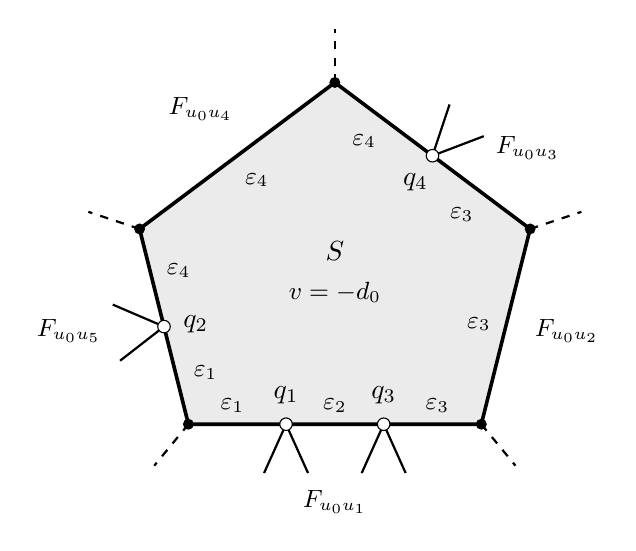
\begin{tikzpicture}[scale=0.62,
  leg/.style={line width=1.3pt},
  stub/.style={line width=0.8pt},
  nodev/.style={circle,draw,fill=white,inner sep=1.6pt},
  posv/.style={circle,fill=black,inner sep=1.4pt}]
  \fill[black!8] (0,4)--(4,1)--(3,-3)--(-3,-3)--(-4,1)--cycle;
  \draw[leg] (0,4)--(4,1)--(3,-3)--(-3,-3)--(-4,1)--cycle;
  \draw[stub,dashed] (0,4)--(0,5.1);
  \draw[stub,dashed] (4,1)--(5.05,1.35);
  \draw[stub,dashed] (3,-3)--(3.7,-3.85);
  \draw[stub,dashed] (-3,-3)--(-3.7,-3.85);
  \draw[stub,dashed] (-4,1)--(-5.05,1.35);
  \draw[stub] (-1,-3)--(-1.45,-4.0); \draw[stub] (-1,-3)--(-0.55,-4.0);
  \draw[stub] (1,-3)--(0.55,-4.0);   \draw[stub] (1,-3)--(1.45,-4.0);
  \draw[stub] (-3.5,-1)--(-4.55,-0.55); \draw[stub] (-3.5,-1)--(-4.4,-1.7);
  \draw[stub] (2,2.5)--(2.35,3.55); \draw[stub] (2,2.5)--(3.05,2.9);
  \foreach \p in {(0,4),(4,1),(3,-3),(-3,-3),(-4,1)} \node[posv] at \p {};
  \node[nodev] at (-1,-3) {}; \node[nodev] at (1,-3) {};
  \node[nodev] at (-3.5,-1) {}; \node[nodev] at (2,2.5) {};
  \node at (-1,-2.4) {$q_1$}; \node at (1,-2.4) {$q_3$};
  \node at (-2.85,-0.95) {$q_2$}; \node at (1.65,1.95) {$q_4$};
  \node at (-2.1,-2.62) {\small$\varepsilon_1$}; \node at (0,-2.62) {\small$\varepsilon_2$}; \node at (2.1,-2.62) {\small$\varepsilon_3$};
  \node at (-2.65,-1.95) {\small$\varepsilon_1$}; \node at (-3.2,0.15) {\small$\varepsilon_4$};
  \node at (-1.6,2.0) {\small$\varepsilon_4$}; \node at (0.6,2.8) {\small$\varepsilon_4$};
  \node at (2.6,1.3) {\small$\varepsilon_3$}; \node at (2.95,-0.95) {\small$\varepsilon_3$};
  \node at (0,-4.6) {\small$F_{u_0u_1}$};
  \node at (4.75,-1.1) {\small$F_{u_0u_2}$};
  \node at (3.95,2.65) {\small$F_{u_0u_3}$};
  \node at (-2.75,3.45) {\small$F_{u_0u_4}$};
  \node at (-5.45,-1.1) {\small$F_{u_0u_5}$};
  \node at (0,0.55) {$S$}; \node at (0,-0.3) {\small$v=-d_0$};
\end{tikzpicture}
\caption{The belt cycle of $X_9$, schematically: the boundary of the facet $F_{u_0}$ seen along $d_0$. The five two-faces
$F_{u_0u_i}$ met by $\partial S$ appear as sides and the five positive vertices of $\partial S$ as corners ($\bullet$); the
four nodes are the circles. Thick lines are the $18$ legs of $\partial S$, labelled by their lower supports
$\varepsilon_1,\dots,\varepsilon_4$; the two other legs at each node and the third leg at each positive vertex (dashed) leave
$F_{u_0}$ and are drawn as stubs. The disc $S$ (shaded) spans $\partial S$ inside $F_{u_0}$, with the constant field
$-d_0$.}\label{fig:x9}
\end{figure}

\emph{The disc.} Let $S$ be the disc bounded by $\partial S$ formed by the $26$ triangles $(b_e,b_f,b_C)$ of the
barycentric subdivision $\mathfrak K_0$ of $\mathscr P$ listed in the accompanying data (\coderepo). Its triangles lie in three maximal
cells of $\mathscr P$, all with facet index $u_0$, and $S$ meets the two-faces of $\nabla^{\check h}$ only along
$\partial S$. Orient $S$ so that $\partial S$ passes through the nodes in the order $q_1,q_2,q_4,q_3$, and give it the
constant field $v=-d_0$.

\begin{lemma}\label{lem:x9belt}
$(S,j,v)$ is a belt cycle, and $\rho(S)=q_1-q_2-q_3+q_4$. In particular $\rho(S)$ generates $K$.
\end{lemma}

\begin{proof}
We check the clauses of \cite[Def.~7.2]{CBM} (Section~\ref{ssec:cbm}). Clauses (a)--(c): $S$ is an embedded disc, a
tropical domain with one sheet and no interior edges or vertices. Its interior lies in the interior of $F_{u_0}$, which
does not meet $\Gamma$, so $j^{-1}(\Gamma)=\partial S$ and $S$ does not cross $\Gamma$. On the interior of $F_{u_0}$ the chart
is the inclusion into $\operatorname{aff}(F_{u_0})$ with tangent lattice $u_0^\perp\cap N$, which contains the primitive
vector $d_0$; so $v$ is a primitive integral parallel field. Clauses (d), (e): $\partial S$ has no vertices, meets no
negative vertex, and follows two opposite legs at each node. Clause (h): every leg of $\partial S$ lies in a two-face
$F_{u_0u_i}$ and has vanishing vector $\pm d_0$ and covector $\pm(u_0-u_i)$. Its monodromy
$x\mapsto x\pm\langle u_0-u_i,x\rangle d_0$ fixes $v$. At the positive vertices all three legs have the vanishing vector
$\pm d_0$, and at the nodes the monodromies of all four legs fix $d_0$, the common direction of the two sides used; so
$v$ is invariant under every monodromy that $\partial S$ meets. Clauses (f), (g), (i) and (j) are void.

For the node coefficients, the boundary network of $v[S]$ is $-d_0[\partial S]$. Along the arcs over
$\varepsilon_1,\varepsilon_4,\varepsilon_3,\varepsilon_2$, oriented by $\partial S$, its canonical lifts (Section~\ref{ssec:tropical}) are
$e_6-e_3$, $e_2-e_7$, $e_5-e_4$ and $e_{10}-e_8$. By Definition~\ref{def:nodecoef}, $\rho_q$ is the coefficient of
$\circv_q$ in the lift after $p_q$ minus the lift before it:
\[
\begin{aligned}
q_2:&\quad (e_2-e_7)-(e_6-e_3)=-\circv_{q_2}, & q_4:&\quad (e_5-e_4)-(e_2-e_7)=\circv_{q_4},\\
q_3:&\quad (e_{10}-e_8)-(e_5-e_4)=-\circv_{q_3}, & q_1:&\quad (e_6-e_3)-(e_{10}-e_8)=\circv_{q_1}.
\end{aligned}
\]
So $\rho(S)=q_1-q_2-q_3+q_4$. Reversing the orientation of $S$, or the sign of $v$, replaces $\rho(S)$ by $-\rho(S)$.
\end{proof}

Everything used here depends on $\mathcal T$ and $\Sigma'$ and not on the height $\check h$: by
Lemma~\ref{lem:indepheight}, for two heights on $\mathcal T$ satisfying the conditions of Theorem~\ref{thm:U} the
decompositions $\mathscr P$ correspond cell by cell, preserving lower supports and face labels, and the induced
homeomorphism of the bases preserves the facets, $\Gamma$ and its legs with their lower supports. So $S$ is a belt cycle
on the base of every such height, the normalised height of Section~\ref{ssec:gross} included, with the same node
coefficients.

\emph{The theorems on $X_9$.} Lemma~\ref{lem:x9belt} proves Theorem~\ref{thm:real} for $X_9$ without the argument of
Section~\ref{sec:cycles}: the chain $v[S]$ lies in $Z(\mathfrak K_0)$, so $K=\Z\rho(S)\subseteq\rho(Z(\mathfrak K_0))$, and the
reverse inclusion is $\rho(\mathrm{Bal}(\Gamma))\subseteq K$, the easy half of the boundary level
(Section~\ref{ssec:cycles-bdry}). The remaining statements take the following
form.
\begin{itemize}
\item \emph{The mirror lift} (Theorem~\ref{thm:lift}). The disc $S$ lifts to an integral $4$-chain $\check\Xi(S)$ on $Y_t$
with
\[
\partial\check\Xi(S)=[\delta_{q_1}]-[\delta_{q_2}]-[\delta_{q_3}]+[\delta_{q_4}].
\]
Over the interior of $S$ it is the bundle of two-tori $\ker v\otimes U(1)$ in the fibres of the mirror torus fibration:
over a point of $S$, the subtorus of the fibre three-torus on which the pairing with $d_0$ vanishes. Near $\partial S$ it
is assembled from pieces cut out by toric divisors of $X_{\mathcal T}$, which add no boundary along the $18$ legs, and at
each of the four nodes it ends on a three-sphere isotopic to $\pm\delta_q$ (Section~\ref{sec:lift}).
\item \emph{The relations} (Theorem~\ref{thm:main}(1)). The relation lattice of the four vanishing spheres is exactly
$\Z(1,-1,-1,1)$, and $\sum_qk_q[\delta_q]$ is torsion only if $k$ is a multiple of $(1,-1,-1,1)$. The classes
$[\delta_{q_1}],\dots,[\delta_{q_4}]$ span a free subgroup of rank three of $H_3(Y_t;\Z)$.
\item \emph{The nodal locus} (Theorem~\ref{thm:main}(3)). Near the given member, the members with a node at each of the
four points $q_P$ form a complex submanifold of codimension $3$: the four nodes impose three conditions, as Morrison's
count predicts for a small resolution of relative Picard number $3$.
\item \emph{Smoothings} (Corollary~\ref{cor:smooth}). The generator of $K$ has every coefficient nonzero. So $X'_9$ has a
smoothing, the vanishing spheres satisfy the relation $[\delta_{q_1}]-[\delta_{q_2}]-[\delta_{q_3}]+[\delta_{q_4}]=0$ with
all coefficients nonzero, and one of the $16$ conifold transitions of $Y_t$ in Lagrangian spheres isotopic to the
$\delta_q$ carries a symplectic structure with symplectic exceptional curves.
\item \emph{The resolution side} (Theorem~\ref{thm:res}). The same disc gives an integral $3$-chain $\Xi(S)$ on a
projective small resolution $\widehat X_9$ with $\partial\Xi(S)=[C_{q_1}]-[C_{q_2}]-[C_{q_3}]+[C_{q_4}]$. So one tropical
object bounds on both sides of the conifold transition, with the same coefficients.
\end{itemize}

\subsection{The examples \texorpdfstring{$X_{19}$}{X19} and \texorpdfstring{$X_{20}$}{X20}}\label{ssec:x19x20}
The polytopes $\Delta_{19}$ and $\Delta_{20}$ of \cite{Paper4} have $19$ and $20$ vertices, one $dP_7$ pentagon each, and
$14$ and $17$ unit squares; so $|Q|=16$ and $|Q|=19$. Both satisfy~\ref{hyp:P}. Their data are in
Appendices~\ref{app:data-x19} and~\ref{app:data-x20}. On each we exhibit tropical $2$-cycles in the sense of
\cite[Def.~7.2]{CBM} whose node coefficients generate $K$ over $\Z$; they illustrate Theorem~\ref{thm:real} and verify
Conjecture~\ref{conj:strict} on these two polytopes. Table~\ref{tab:x19x20} lists them. Besides belt cycles there are
cycles whose boundary graph has trivalent vertices; these vertices are negative vertices of $\Gamma$, and the boundary
graphs are a complete graph on four vertices ($X_{19}$) and two vertices joined by three paths ($X_{20}$).

\begin{table}[ht]
\centering\small
\begin{tabular}{lllp{7.3cm}}
& cycle & boundary graph & node coefficients $\rho(S_i)$\\\hline
$X_{19}$ & $S_1$ & closed path, $4$ nodes & $q_2-q_3+q_4-q_7$\\
 & $S_2$ & complete graph on $4$ vertices & $q_1+q_3-q_4-q_5-q_8-q_9+q_{11}+q_{12}+q_{14}-q_{15}$\\
 & $S_3$ & complete graph on $4$ vertices & $q_2-q_3-q_6+q_8-q_9+q_{10}+q_{11}-q_{12}-q_{13}+q_{16}$\\[2pt]
$X_{20}$ & $S_1$ & closed path, $3$ nodes & $-q_{14}+q_{16}-q_{17}$\\
 & $S_2$ & closed path, $3$ nodes & $q_3-q_4+q_{14}$\\
 & $S_3$ & closed path, $4$ nodes & $-q_4+q_5-q_9+q_{10}$\\
 & $S_4$ & closed path, $3$ nodes & $q_2-q_5+q_{13}$\\
 & $S_5$ & closed path, $3$ nodes & $-q_{13}+q_{16}-q_{19}$\\
 & $S_6$ & two vertices, three paths & $q_4-q_5+q_7-q_8+q_{11}-q_{12}+q_{15}-q_{18}$
\end{tabular}
\caption{Tropical $2$-cycles on $X_{19}$ ($|Q|=16$, $\operatorname{rank}K=3$) and $X_{20}$ ($|Q|=19$,
$\operatorname{rank}K=6$) whose node coefficients generate $K$; the cycles with a closed path as boundary are belt cycles.
In the $\Z$-bases of $K$ of Appendix~\ref{app:data} the matrices of the $\rho(S_i)$ have all elementary divisors equal to
$1$.}\label{tab:x19x20}
\end{table}

The two examples differ in the conclusion of Corollary~\ref{cor:smooth}.
\begin{itemize}
\item On $X_{19}$ no node is forced on $K$. For instance
$\lambda=3\rho(S_1)+2\rho(S_2)+\rho(S_3)$, that is
\[
\begin{aligned}
\lambda={}&2q_1+4q_2-2q_3+q_4-2q_5-q_6-3q_7-q_8\\
&-3q_9+q_{10}+3q_{11}+q_{12}-q_{13}+2q_{14}-2q_{15}+q_{16},
\end{aligned}
\]
lies in $K$ and has all $16$ coefficients nonzero. So $X'_{19}$ has a smoothing, and $\sum_q\lambda_q[\delta_q]=0$ is a
relation among the vanishing spheres of the mirror with every coefficient nonzero.
\item On $X_{20}$ the two pentagon nodes $q_1$ and $q_6$ occur in no relation: the basis of $K$ in
Appendix~\ref{app:data-x20} has coordinate $0$ at both. By Corollary~\ref{cor:smooth}, $X'_{20}$ has no smoothing, and
although $\operatorname{rank}K=6$, no relation among the $19$ vanishing spheres of the mirror has all coefficients
nonzero.
\end{itemize}
In both cases $|Q|-\operatorname{rank}K=13$, the codimension of the nodal locus in Theorem~\ref{thm:main}(3).

\subsection{Hexagon examples}\label{ssec:hexexamples}
We give one example on each branch of the $dP_6$ hexagon. On both, the centre $o$ of the hexagon occurs only in the
circuits of the nodes of the hexagon, each time with coefficient $-1$ in the labelling with the diagonal through the
centre, so every $\lambda\in K$ satisfies the tie $\sum_{q\text{ at }G}\lambda_q=0$ at the hexagon $G$. The data are in
Appendix~\ref{app:data-hex}.

\emph{$X_{88}$, the $A_1$ branch.} The polytope $\Delta_{88}$ has $21$ vertices, $22$ unit squares, one hexagon and no
pentagon. All three $A_1$ tilings of the hexagon satisfy~\ref{hyp:P}, and neither $A_2$ tiling does. On the $A_1$ profile
of Appendix~\ref{app:data-hex}, $X'_\sigma$ has $|Q|=24$ nodes, two of them at the hexagon, and $\operatorname{rank}K=10$. The
two hexagon nodes share only the centre, their carrying cells lie in one two-face of $\nabla^{\check h}$, and the
tie reads $\lambda_{q_{23}}+\lambda_{q_{24}}=0$. On the resolution side the exceptional surface over the centre is a
$dP_6$ surface, the curves $C_{q_{23}}$ and $C_{q_{24}}$ are two opposite $(-1)$-curves in its hexagon of lines, and its
image in $X'_\sigma$ is $\mathbb P^1\times\mathbb P^1$, with the two nodes at opposite torus-fixed points
(Proposition~\ref{prop:classical}). No node is forced on $K$: the vector
\[
\begin{aligned}
&-q_1+q_2-2q_3-q_4+q_5+q_6-q_7+q_8-2q_9+q_{10}-q_{11}+2q_{12}-2q_{13}\\
&\qquad-q_{14}-q_{15}-q_{16}+q_{17}-q_{18}-q_{19}+q_{20}+q_{21}-q_{22}+q_{23}-q_{24}
\end{aligned}
\]
lies in $K$. So $X'_{88}$ has a smoothing, and the nodal locus of the mirror has codimension $14$. Ten tropical $2$-cycles
in the sense of \cite[Def.~7.2]{CBM} have node coefficients generating $K$ with index one: six belt cycles, two cycles
whose boundary graph has two trivalent vertices joined by three paths, one whose boundary graph is a complete graph on
four vertices, and one whose boundary network was found by integer programming and which crosses $\Gamma$ transversally
at $18$ points. The six belt cycles satisfy Definition~\ref{def:belt}: they are discs with one field that meet $\Gamma$
only along their boundary. Two of the ten pass through the hexagon nodes, with node coefficients $\pm(1,-1)$ there, as the tie requires.

\emph{$X_{154}$, the $A_2$ branch.} The polytope $\Delta_{154}$ has $22$ vertices, $20$ unit squares, one hexagon and no
pentagon. No $A_1$ tiling of the hexagon satisfies~\ref{hyp:P}, and both $A_2$ tilings do; on the $A_1$ branch two nodes
would moreover be forced on $K$. On the $A_2$ profile of Appendix~\ref{app:data-hex}, $|Q|=23$, three nodes lie at the
hexagon, and $\operatorname{rank}K=9$. Among the polytopes of the list that satisfy~\ref{hyp:P} with every hexagon on the
$A_2$ branch and have no forced node, it has the smallest $|Q|$ and the smallest rank of $K$. The tie reads
$\lambda_{q_{21}}+\lambda_{q_{22}}+\lambda_{q_{23}}=0$, and the projection of $K$ to these three coordinates is the whole
lattice $\{\lambda\in\Z^3:\lambda_1+\lambda_2+\lambda_3=0\}$. Here the three exceptional curves at the hexagon are three
pairwise disjoint $(-1)$-curves of the $dP_6$ surface over the centre, whose image in $X'_\sigma$ is $\mathbb P^2$ with the
three nodes at its torus-fixed points (Proposition~\ref{prop:classical}). No node is forced; the vector
\[
\begin{aligned}
&-q_1+q_2+2q_3+q_4-2q_5+2q_6-q_7+q_8-q_9-q_{10}+q_{11}+q_{12}\\
&\qquad+2q_{13}+q_{14}-q_{15}-q_{16}+q_{17}+q_{18}-q_{19}+2q_{20}+q_{21}+q_{22}-2q_{23}
\end{aligned}
\]
lies in $K$, so $X'_{154}$ has a smoothing, which the $A_1$ branch does not see, and the nodal locus of the mirror has
codimension $14$.

The discriminant at the $A_2$ hexagon has a feature that the other examples do not have. The three node parallelograms
share pairwise an edge $[o,w]$ through the centre, and their carrying cells lie in one two-face of $\nabla^{\check h}$. At
each node two of the four legs have lower support $\{o,w\}$ for such an edge, and these two legs are adjacent. The legs
with lower support $\{o,w\}$ join the two nodes that share $[o,w]$ by a path of $\Gamma$ through two-valent points only,
with constant vanishing vector $\pm(w-o)$; on $B$ these paths have $2$, $4$ and $4$ legs. The three paths form a cycle of
$\Gamma$ that contains no trivalent vertex. Nine belt cycles, each a disc with one field meeting $\Gamma$ only along its
boundary, have node coefficients generating $K$ with index one. Four of
them pass through two of the three hexagon nodes each: the boundary enters along a leg outside the two-face, passes
$q_i$, runs along the path of $\Gamma$ from $q_i$ to $q_j$, and leaves along a leg outside the two-face. Their node
coefficients at the three hexagon nodes are roots of the tie plane, $\pm(1,0,-1)$ and $\pm(0,1,-1)$ up to the order of
the nodes, and they span it.

\subsection{The list}\label{ssec:list}
The \emph{list} is the following set of $\NVertexSets$ vertex sets of reflexive four-polytopes:
\begin{itemize}
\item the $77$ admissible reflexive four-polytopes with at most nine vertices that have a pentagonal two-face
\cite{Paper4}, together with $\Delta_{19}$ and $\Delta_{20}$, and the polytope $X^\circ$ of \cite{Paper4};
\item the reflexive four-polytopes $\Delta$ for which every edge of $\Delta$ and of $\Delta^\circ$ is primitive, determined in
\cite{Paper3} by a scan of the $473{,}800{,}776$ reflexive four-polytopes of the classification of Kreuzer and Skarke
\cite{KS00};
\item the product of two reflexive hexagons, with $36$ vertices \cite{Paper3}.
\end{itemize}
Of these, $\NAdmSets$ are admissible (Definition~\ref{def:admissible}), and they form $\NAdm$ polytopes up to $GL_4(\Z)$:
the only coincidence is that $X^\circ$ is equivalent to a polytope of the second item. All $\NAdm$ occur among the
admissible polytopes of the Kreuzer--Skarke list found in Appendix~\ref{app:unimodular}.
Table~\ref{tab:list} gives the counts.

\begin{table}[ht]
\centering\small
\begin{tabular}{lrr}
& polytopes & \ref{hyp:P} for some profile\\\hline
admissible, no hexagonal two-face & $\NHexFree$ & \\
\quad no singular two-face & $\NHexFreeSmooth$ & \\
\quad some singular two-face, $K=0$ & $\NHexFreeKzero$ & \\
\quad $K\neq0$ & $\NList$ & $\NScope$\\
admissible, some hexagonal two-face & $\NHex$ & $\NHexProj$\\
\quad every hexagon on the $A_1$ branch & & $\NHexAone$\\
\quad every hexagon on the $A_2$ branch & & $\NHexAtwo$\\
\quad mixed profiles & & $\NHexMixed$
\end{tabular}
\caption{The admissible polytopes of the list, up to $GL_4(\Z)$. For hexagon-free polytopes the profile is unique. In
each of the last three rows a polytope is counted if~\ref{hyp:P} holds for some profile of that kind, so a polytope may be
counted in several of them.}\label{tab:list}
\end{table}

\emph{Hypothesis~\ref{hyp:P}.} It is a linear feasibility problem over $\Q$ in the heights of the lattice points of
$\partial\Delta$ (Section~\ref{ssec:proj}), which we decide exactly: a feasible profile is certified by an integral
solution, an infeasible one by a Farkas certificate verified in exact rational arithmetic. For a polytope with
$h$ hexagons, whether~\ref{hyp:P} holds for some profile with every hexagon on the $A_1$ branch, for some with every
hexagon on the $A_2$ branch, and for some mixed profile, is decided by a depth-first search over the $5^h$ profiles in
which a certificate for a partial choice of tilings excludes all its completions. On the hexagon-free polytopes with $K\ne0$, \ref{hyp:P} fails on
$\NPfail$ of $\NList$, all with a pentagonal two-face. On the $\NHex$ polytopes with a hexagon it holds for some profile
on $\NHexProj$ and for none on $\NHexNoProj$; the branch patterns are counted in Table~\ref{tab:list}. Where~\ref{hyp:P} fails there is an exact certificate: an effective combination of curves
contracted by $X'_\sigma\to X$ that is numerically a combination of exceptional curves (Section~\ref{ssec:proj}). The
polytopes of the list with $K\neq0$ to which Theorems~\ref{thm:main}--\ref{thm:res} apply are therefore the
$\NScope+\NHexProj=\NScopeAll$ polytopes of the last column; on every profile of a hexagonal polytope examined, $K\ne0$. (Of the $\NHexSets$ admissible vertex sets with a hexagon, $X^\circ$ and its equivalent both fail
\ref{hyp:P} on every profile.)

\emph{Theorem~\ref{thm:real} on the list.} Theorem~\ref{thm:real} is proved in Section~\ref{sec:cycles}; the following
computation corroborates it and is not used in the proof. On the bases of the $\NScope$ hexagon-free polytopes in scope
and, in addition, on the bases of $X_9$, $X_{19}$, $X_{20}$ built from the heights in the accompanying data
(\coderepo; $\NThmCBases$ bases, with $\operatorname{rank}K$ between $1$ and $36$ and up to $60$ nodes) we computed a
basis of the group $\mathrm{Bal}(\Gamma)$ of balanced networks, checked $\rho(\mathrm{Bal}(\Gamma))=K$ by a Smith normal
form, and showed, by solving the integral linear systems exactly, that every balanced network is the boundary network
of an integral relative tropical $2$-cycle on $\mathfrak K_0$. On every base $\partial Z(\mathfrak K_0)=\mathrm{Bal}(\Gamma)$
and $\rho(Z(\mathfrak K_0))=K$ with index one. On $\NThmCGlobal$ of the
bases the balanced networks contained in the boundary of a single facet $F_u$, which bound inside $F_u$, have node
coefficients spanning a proper sublattice of $K$, so that the global argument of Section~\ref{sec:cycles} is needed
there. The same computation succeeds on $\NThmCHexBases$ bases
of $\NHexProfAtwo$ polytopes with hexagonal two-faces: the $\NHexProfAtwo$ polytopes with a profile satisfying~\ref{hyp:P}
on the $A_2$ branch or a mixed one, each on one such profile, and in addition the product of two hexagons on an $A_1$
profile. It was not run on the $12$ polytopes whose profiles satisfying~\ref{hyp:P} are all on the $A_1$ branch; $X_{88}$ is
one of them.

\emph{Forced nodes and Corollary~\ref{cor:smooth}.} A node $q$ is \emph{forced} on $K$ if $\lambda_q=0$ for every
$\lambda\in K$, that is, if the $q$-th coordinate vanishes on a $\Z$-basis of $K$. Since a lattice is not a finite union
of sublattices of smaller rank, some $\lambda\in K$ has every $\lambda_q\neq0$ if and only if no node is forced; this is
condition~(b) of Corollary~\ref{cor:smooth}. At a hexagon the forced nodes depend on the profile only through its branch:
the three $A_1$ tilings give the same centre-free combination $\pm(e_{w_0}-e_{w_1}+e_{w_2}-e_{w_3}+e_{w_4}-e_{w_5})$ of
their two circuits, and the two $A_2$ tilings give the same plane of centre-free combinations of their three circuits,
with the same three lines on which one node coefficient vanishes (Remark~\ref{rem:tie}). We computed a
$\Z$-basis of $K$ and the forced nodes in exact integer arithmetic for every polytope in scope and every branch pattern
on which~\ref{hyp:P} holds. For a polytope with several hexagons we first test the profiles found by the search for
\ref{hyp:P}; where each of them has a forced node, an exact search of the same kind over all profiles whose branch
pattern has no forced node decides whether one of them satisfies~\ref{hyp:P}; for the count by mixed profiles the same
search is run over the mixed patterns without forced node whenever the mixed profile found first has a forced node. The
result:
\begin{itemize}
\item among the $\NScope$ hexagon-free polytopes in scope, condition~(b) holds on $\NCorBHexFree$;
\item among the $\NHexProj$ hexagonal polytopes in scope, it holds for some profile satisfying~\ref{hyp:P} on
$\NCorBHex$: on $\NCorBHexOne$ of the $\NHexOne$ with one hexagon and on $\NCorBHexMany$ of the $\NHexMany$ with several.
By branch pattern, it holds on $\NCorBAoneWit$ of the $\NHexAone$ polytopes with an $A_1$ profile satisfying~\ref{hyp:P},
on $\NCorBAtwoWit$ of the $\NHexAtwo$ with an $A_2$ profile, and on $\NCorBMixedWit$ of the $\NHexMixed$ with a mixed
profile.
\end{itemize}
So on $\NCorBAll$ of the $\NScopeAll$ polytopes in scope, $X'_\sigma$ has a smoothing for some profile, and for that
profile the vanishing spheres of the mirror satisfy a relation with every coefficient nonzero. On the other
$\NCorBFail$ every profile satisfying~\ref{hyp:P} has a forced node; by Corollary~\ref{cor:smooth}, $X'_\sigma$ then has no
smoothing and every relation among the $\delta_q$ has a zero coefficient. The programs for these computations are
available at \coderepo.

\subsection{Evidence for Conjecture~\ref{conj:strict}}\label{ssec:evidence}
Conjecture~\ref{conj:strict} asks for more than Theorem~\ref{thm:real}: that tropical $2$-cycles in the strict sense of
\cite[Def.~7.2]{CBM}, whose fields are primitive, whose interior edges and crossings with $\Gamma$ are of the restricted
kinds that definition allows, and whose boundaries pass each node at most once along two opposite legs, already have node
coefficients generating $K$. It is the lattice form, for the bases $B'_\sigma$, of the
conjecture of Casta\~no-Bernard and Matessi that every good relation among the vanishing cycles is a combination of
relations coming from tropical $2$-cycles \cite[\S1, Conj.~8.3]{CBM}. We tested it on the $\NScope$ hexagon-free
polytopes of the list in scope, each on the base built from a height of Theorem~\ref{thm:U}.

The evidence separates the boundary of a tropical $2$-cycle from its interior. By clauses (d), (e) and (h) of
\cite[Def.~7.2]{CBM}, the boundary network of a strict tropical $2$-cycle has the following form.

\begin{definition}[CBM-shaped networks]\label{def:cbmshaped}
A balanced network $h=\sum_Ec_E\,d_E[E]$ is \emph{CBM-shaped} if every $c_E\in\{0,\pm1\}$, the legs with $c_E\ne0$ meet
every node in none or in two opposite legs, meet every negative vertex in none or all three legs, and meet every other
point of $\Gamma$ in at most two legs. Its negative vertices with three legs are its \emph{trivalent vertices}.
\end{definition}

A CBM-shaped network is a balanced network in the sense of Section~\ref{ssec:tropical} whose support is a graph of the
kind that the boundary of a tropical $2$-cycle of \cite{CBM} can have; its node coefficients lie in $K$ by
Theorem~\ref{thm:real}. Conjecture~\ref{conj:strict} asserts in particular that CBM-shaped networks generate $K$, and in
addition that enough of them bound strict tropical $2$-cycles. The strict cycles were constructed from a boundary
network $h$ in three steps: the germ of the cycle along $h$ is found by an integer program in the coefficients of the
triangles of $\mathfrak K_0$ that meet the support of $h$, subject to the clauses of \cite[Def.~7.2]{CBM} along the
boundary and with coefficients $0,\pm1$; the germ is filled by an integral relative tropical $2$-cycle, found by an
integer program and checked in exact arithmetic; and near each point of $\Gamma$ where the filling violates a clause of
\cite[Def.~7.2]{CBM}, the filling is replaced, on the second barycentric subdivision, by a chain with constant coefficient
in the lattice of vectors invariant under the local monodromy. Every cycle obtained was checked against every clause of
\cite[Def.~7.2]{CBM} by two independently written programs. On the $\NScope$ polytopes we find the following.

\begin{enumerate}
\item[(a)] \emph{Boundaries.} On all $\NScope$ polytopes, the node coefficients of CBM-shaped networks generate $K$, as
the Smith normal form of their matrix in a basis of $K$ shows. Networks without trivalent vertices, networks with two
trivalent vertices joined by three paths and networks whose trivalent vertices form a complete graph on four vertices
suffice on $\NBdryEnum$ polytopes; on the other $\NBdryIP$ further CBM-shaped networks found by integer programming
are needed.
\item[(b)] \emph{Belt cycles.} Networks without trivalent vertices generate $K$ on $\NMinNegZero$ polytopes. On
$\NBelts$ of these, strict tropical $2$-cycles whose domain is a disc with one constant field and whose boundary network is
a single closed path generate $K$; on $\NBeltsStrict$ they can all be taken to be belt cycles (Definition~\ref{def:belt}),
while on the other $\NBeltsCrossPoly$ some of the discs used cross $\Gamma$ transversally at interior points of legs, as
\cite[Def.~7.2]{CBM} allows. We checked each of the $\NBeltsChecked$ discs of this kind that were constructed: all are
discs with one field up to sign, and $\NBeltsCross$ of them meet $\Gamma$ off their boundary.
\item[(c)] \emph{Strict cycles.} On $\NRealised$ polytopes, $X_9$, $X_{19}$ and $X_{20}$ among them, there are strict
tropical $2$-cycles whose node coefficients generate $K$; the index of the lattice they span in $K$ was computed exactly
and is one.
\item[(d)] \emph{The remaining polytopes.} On the other $\NRemaining$ polytopes the strict cycles constructed generate a
sublattice of $K$ of corank between $1$ and $\NCorankMax$, and of corank one on $\NCorankOne$. For each CBM-shaped network
of a generating set that is not the boundary of a constructed cycle, the construction meets an obstruction of one of
three kinds:
\begin{enumerate}
\item[(1)] \emph{a single sheet:} a network without trivalent vertices, with vanishing vector $\pm d$, is not known to
bound a disc with field $\pm d$ formed by triangles of $\mathfrak K_0$ that lie in facets $F_u$ with $\langle u,d\rangle=0$
and meet $\Gamma$ only along the network and at edge points; it may still bound a cycle with several sheets;
\item[(2)] \emph{the filling:} the germ has an integral filling, but none is known that satisfies, near the points of
$\Gamma$ off the network, the conditions under which the local replacement applies;
\item[(3)] \emph{the local replacement:} near some point of $\Gamma$ off the network, or at an interior vertex of the
cycle, no constant coefficient of small norm in the invariant lattice removes the violation of the clauses of
\cite[Def.~7.2]{CBM}.
\end{enumerate}
Each kind occurs, for some network, on $\NFailSheet$, $\NFailFill$ and $\NFailLocal$ of the $\NRemaining$ polytopes
respectively.
\item[(e)] \emph{Trivalent vertices appear to be needed.} Let $k(X)$ be the least $k$ such that the CBM-shaped networks with at
most $k$ trivalent vertices generate $K$. Then $k(X)=0$ exactly on the $\NMinNegZero$ polytopes of (b), and on the other
$\NMinNegPos$ the computations suggest $k(X)=2,4,6,8$ on $\NMinNegTwo$, $\NMinNegFour$, $\NMinNegSix$ and $\NMinNegEight$
polytopes respectively. The upper bounds are explicit networks; each lower bound $k(X)>k$ with $k\ge2$ rests on the
infeasibility, computed in floating-point arithmetic, of an integer program asking for a CBM-shaped network with at most
$k$ trivalent vertices whose node coefficients lie outside a hyperplane of $K\otimes\Q$ containing those of all networks
without trivalent vertices. For $X_9$, $X_{19}$ and $X_{20}$ the values so obtained are $k(X)=0,4,2$, in accordance with
Table~\ref{tab:x19x20}.
\end{enumerate}
On the hexagonal polytopes in scope, strict cycles constructed in the same way generate $K$ with index one on
$\NHexRealAone$ of the $\NHexAone$ polytopes with an $A_1$ profile satisfying~\ref{hyp:P} and on $\NHexRealAtwo$ of the
$\NHexProfAtwo$ with an $A_2$ or mixed profile, each on one profile; on the other six the construction stopped with a
sublattice of smaller rank or at its time limit.

The obstructions of (d) sit in the passage from a CBM-shaped network to a strict cycle, not at the boundary level, where
(a) holds everywhere; and by (e) a proof of Conjecture~\ref{conj:strict} cannot restrict itself to networks with few
trivalent vertices. The relative tropical $2$-cycles of Theorem~\ref{thm:real} avoid all three obstructions: they allow
several sheets, arbitrary branching along edges and crossings of $\Gamma$ with any invariant coefficient, which is what the
filling of Section~\ref{sec:cycles} uses.


\appendix
\section{Unimodular heights: proof of Theorem~\ref{thm:U}}\label{app:unimodular}

Theorem~\ref{thm:U} asks, for every admissible $\Delta$, for a unimodular triangulation $\mathcal T$ of $\partial\Delta^\circ$
refining its faces and an integral height $\check h$ on the fan over $\mathcal T$ such that $\check h$ and
$\check h-\check\varphi$ are strictly convex. Section~\ref{ssec:ureform} shows that this is equivalent to the existence of
a fine, regular, unimodular triangulation of $\Delta^\circ$ that is star-shaped from the origin, and that strict convexity
of $\check h-\check\varphi$ implies that of $\check h$. Section~\ref{ssec:ufacets} explains why admissibility does not
yield such a triangulation by a general argument: it constrains the facets of $\Delta^\circ$ only along their edges, and
lattice polytopes of dimension three need not have unimodular triangulations at all. Section~\ref{ssec:uproof} proves the
theorem by exhaustion over the classification of Kreuzer and Skarke, with a certificate for each polytope checked in
exact integer arithmetic, and Section~\ref{ssec:utrust} states on what the proof rests.

Throughout, a piecewise linear function $g$ on a complete simplicial fan is \emph{strictly convex} if it is convex and its
maximal domains of linearity are the maximal cones. A \emph{wall} is a common facet of two maximal cones $\kappa,\kappa'$,
and the \emph{bend} of $g$ across it is $g(m')-\ell_\kappa(m')$, where $\ell_\kappa$ is the linear function equal to $g$ on
$\kappa$ and $m'$ is the generator of $\kappa'$ not in $\kappa$. Bends are additive in $g$, and $g$ is strictly convex if
and only if every bend is positive; this is the wall criterion of \cite[\S6.1]{CLS}, where support functions carry the
opposite sign, so that convexity here is concavity there. Recall that $\check\varphi$ equals $1$ on $\partial\Delta^\circ$ and is
linear on the cones over the faces of $\Delta^\circ$; it is convex, its maximal domains of linearity are the cones over the
facets, and $\check\varphi(m)=\max_v\langle m,-v\rangle$ over the vertices $v$ of $\Delta$.

\subsection{Reformulation}\label{ssec:ureform}

\begin{lemma}\label{lem:Ureform}
Let $\mathcal T$ be a unimodular triangulation of $\partial\Delta^\circ$ refining its faces. The following are
equivalent.
\begin{enumerate}
\item[(a)] There is a piecewise linear function $\check h$ on the fan over $\mathcal T$, integral on $M$, such that $\check h$ and
$\check h-\check\varphi$ are strictly convex.
\item[(b)] There is a real piecewise linear function on the fan over $\mathcal T$ that is strictly convex.
\item[(c)] There are real heights $\omega$ on the vertices of $\mathcal T$ such that for every facet $F$ of $\Delta^\circ$ the
restriction $\mathcal T|_F$ is the regular subdivision of $\operatorname{vert}(\mathcal T)\cap F$ induced by $\omega|_F$.
\end{enumerate}
Moreover, for any piecewise linear $\check h$ on the fan over $\mathcal T$, strict convexity of $\check h-\check\varphi$
implies strict convexity of $\check h$.
\end{lemma}

\begin{proof}
(a)$\Rightarrow$(b): take $\check h-\check\varphi$.

(b)$\Rightarrow$(a): strict convexity is an open condition on the values at the rays, so we may take the strictly convex
function $g$ rational, and after scaling integral at the primitive generators of the rays. Put $\check h=g+\check\varphi$.
Then $\check h-\check\varphi=g$ is strictly convex. Every simplex of $\mathcal T$ lies in a facet, so $\check\varphi$ is
linear on every cone of the fan and bends by $\ge0$ across every wall; hence every bend of $\check h$ is at least the
corresponding bend of $g$, and $\check h$ is strictly convex. The same computation proves the last assertion, for any triangulation. The
function $g$ is integral on $M$, because a linear function on a unimodular cone that is integral at the generators is
integral on the lattice points of the cone, and $\check\varphi$ is integral on $M$ because the vertices of $\Delta$ are
lattice points.

(b)$\Rightarrow$(c): put $\omega=g|_{\operatorname{vert}\mathcal T}$. On the cone over a facet $F$, $g$ is convex with the cones
over the simplices of $\mathcal T|_F$ as its maximal domains of linearity. Its restriction to the affine hyperplane of $F$
is therefore a convex piecewise linear function on $F$ whose domains of linearity are exactly the simplices of
$\mathcal T|_F$ and whose values at their vertices are $\omega$; this says that $\mathcal T|_F$ is the regular subdivision
induced by $\omega|_F$.

(c)$\Rightarrow$(b): let $g_0$ be linear on each cone of the fan over $\mathcal T$ with $g_0=\omega$ on the vertices. Across a
wall inside the cone over a facet $F$, the bend of $g_0$ is positive by the regularity of $\mathcal T|_F$, since a bend is
a local condition, homogeneous of degree one. Across the finitely many walls between the cones over two different facets,
$\check\varphi$ bends positively, while it does not bend across walls inside a facet cone. So $g_0+\lambda\check\varphi$
is strictly convex for $\lambda\gg0$.
\end{proof}

Adding a constant to the heights $\omega$ on $\partial\Delta^\circ$ adds a multiple of $\check\varphi$ to the corresponding
piecewise linear function; this is the conversion used below. A triangulation of $\Delta^\circ$ is \emph{star-shaped from
the origin} if the origin is a vertex of each of its maximal simplices.

\begin{corollary}\label{cor:Ureform}
The conclusion of Theorem~\ref{thm:U} holds for $\Delta$ if and only if $\Delta^\circ$ has a fine, regular, unimodular
triangulation that is star-shaped from the origin.
\end{corollary}

\begin{proof}
A star-shaped triangulation of $\Delta^\circ$ consists of the simplices $\operatorname{conv}(0,\tau)$, $\tau$ in a
triangulation $\mathcal T$ of $\partial\Delta^\circ$; each $\tau$ lies in a facet, since a convex subset of the boundary of a
polytope lies in a facet, so $\mathcal T$ refines the faces of $\Delta^\circ$. Since $\Delta^\circ$ is reflexive, every facet lies at lattice distance
one from the origin, so $\operatorname{conv}(0,\tau)$ is unimodular if and only if $\tau$ is unimodular in its facet, and a
unimodular simplex contains no lattice points other than its vertices, so unimodular triangulations are fine. The
star-shaped triangulation is regular if and only if it is induced by heights $0$ at the origin and $\omega$ on
$\partial\Delta^\circ$ (subtract an affine function), and the lower envelope of the lifted points is then linear on each
$\operatorname{conv}(0,\tau)$ and $0$ at the origin; so regularity holds if and only if the piecewise linear function with
values $\omega$ on the fan over $\mathcal T$ is strictly convex. This is (b) of Lemma~\ref{lem:Ureform}, which is equivalent to (a).
\end{proof}

\subsection{The facets of \texorpdfstring{$\Delta^\circ$}{the polar polytope}}\label{ssec:ufacets}
Let $v$ be a vertex of $\Delta$ with neighbours $w_1,\dots,w_k$ along edges, and $d_i=w_i-v$, primitive by admissibility.
The facet of $\Delta^\circ$ dual to $v$ is the lattice three-polytope
\[
F_v=\{m\in M_\R:\ \langle m,v\rangle=-1,\ \langle m,d_i\rangle\ge0\ (i=1,\dots,k)\},
\]
the polytope of the anticanonical bundle of $\mathbb P_\Delta$ restricted to the toric divisor $D_v$. Its vertices, edges
and two-faces correspond to the facets, two-faces and edges of $\Delta$ that contain $v$.

\begin{proposition}\label{prop:Ufacets}
Let $\Delta$ be admissible and let $E$ be an edge of $F_v$, dual to a two-face $\theta\ni v$ of $\Delta$.
\begin{enumerate}
\item The normal cone of $F_v$ along $E$ is lattice equivalent to the tangent cone of $\theta$ at $v$, in the lattice of the
plane of $\theta$. It is unimodular if $\theta$ is a triangle, a square or a hexagon, and if $\theta$ is a pentagon and $v$
is one of its three corners of index one; at the other two corners of a pentagon it has index $2$.
\item If $\theta$ is not a triangle, $E$ has lattice length one.
\end{enumerate}
\end{proposition}

\begin{proof}
(1) The two-dimensional cone of the fan $\operatorname{Star}(v)/v$ given by $\theta$ is $\operatorname{cone}(\theta-v)$ modulo
$\R v$. Since $\theta$ lies in a facet of $\Delta$ at lattice height one, the saturated lattice of $\R\theta$ is
$\Z v\oplus L_\theta$, with $L_\theta$ the direction lattice of the plane of $\theta$, so $L_\theta$ maps isomorphically onto a
saturated sublattice of $N/\Z v$, carrying the tangent cone of $\theta$ at $v$ to that two-dimensional cone. The index at a
corner is the determinant of the two primitive edge vectors there; for the pentagon
$\operatorname{conv}\{(1,0),(1,1),(0,1),(-1,0),(0,-1)\}$ these are $1,1,1,2,2$, for the hexagon all are $1$. (2) is the
condition $\ell(\theta^\circ)=1$ of Definition~\ref{def:admissible}.
\end{proof}

Admissibility is a condition on the two-faces of $\Delta$ and on their dual edges, that is, on the edges of the facets
$F_v$ and on the normal cones along them; Proposition~\ref{prop:Ufacets} records what it says there. It imposes no direct
condition on the cones of $F_v$ at its vertices beyond their two-dimensional faces, nor on the two-faces of $F_v$.

The known sufficient conditions for unimodular triangulations do not apply to these facets. If every facet $F_v$ has
lattice width one with respect to each of its facet normals (is \emph{compressed}), then every pulling triangulation
of each facet is unimodular \cite[Thm.~2.3]{HPPS}, and pulling the boundary lattice points of $\Delta^\circ$ in one global
order gives heights as in Lemma~\ref{lem:Ureform}(c). If the facet normals of a facet form a unimodular matrix, that facet
has a regular unimodular triangulation \cite[Thm.~2.4]{HPPS}, but the triangulations of two adjacent facets obtained in this
way need not agree on the common face. Compressed facets are rare: of the $3{,}175$ facets of the $418$ admissible
polytopes with at most eight vertices, $46$ are compressed. Facets with unimodular normals are common ($12{,}350$ of the
$13{,}469$ facets of the admissible polytopes of the list of Section~\ref{ssec:list}), but their triangulations need not be
compatible. The facets are also far from small: among the $3{,}175$ there are facets with $242$ lattice points and
normalised volume $756$, and $2{,}171$ of the $2{,}444$ facets with at most $40$ lattice points contain empty lattice
tetrahedra of volume greater than one among their lattice points, so that a fine triangulation of such a facet need not be
unimodular. For lattice
three-polytopes in general, unimodular triangulations need not exist, and their existence is open even for smooth
lattice three-polytopes \cite[\S1.5.1]{HPPS}; the facets $F_v$ need not be smooth, since by
Proposition~\ref{prop:Ufacets} their vertex cones are constrained only through their two-dimensional faces. A general
proof of Theorem~\ref{thm:U} would therefore produce compatible regular unimodular triangulations for a class of lattice
three-polytopes, the polytopes of $-K_{\mathbb P_\Delta}|_{D_v}$, for which no such result is known. We know no conceptual
proof, and we prove the theorem by exhaustion.

\subsection{Proof of Theorem~\ref{thm:U}}\label{ssec:uproof}
The proof has three steps: the list of all reflexive four-polytopes, the determination of the admissible ones, and an
exactly checked certificate for each of these.

\emph{Step 1: the classification.} Kreuzer and Skarke classified the reflexive four-polytopes up to $GL_4(\Z)$: there are
$473{,}800{,}776$ of them \cite{KS00}. We use a copy of their list whose completeness we checked against the published
count, with every polytope reflexive and no two equivalent (by normal forms). Every polytope of the list is treated as
$\Delta$; since the list contains the polar of each of its members, this covers every polar pair in both orders.

\emph{Step 2: the admissible polytopes.} Admissibility is decided from the vertices and the facet inequalities of
$\Delta$, computed with PALP \cite{PALP}. The two-faces of $\Delta$ are the maximal vertex sets shared by two facets; each is
classified in the lattice of its plane. By Pick's theorem, a lattice polygon with primitive edges is a unimodular
triangle, a unit square, a $dP_7$ pentagon or a $dP_6$ hexagon exactly when its number of vertices and twice its area are
$(3,1)$, $(4,2)$, $(5,5)$ or $(6,6)$. For every non-triangular two-face the lattice length of the dual edge is computed
from the two facet normals. The result is Table~\ref{tab:Ucounts}: up to $GL_4(\Z)$ there are $51{,}827$ admissible
polytopes, $40{,}403$ without and $11{,}424$ with a hexagonal two-face, and $741$ of them have no singular two-face. Every one of them was checked admissible a second time by an independent
program, the $51{,}827$ have pairwise different normal forms, and the $612$ admissible polytopes of the list of
Section~\ref{ssec:list} all occur among them.

\begin{table}[ht]
\centering\small\setlength{\tabcolsep}{4pt}
\begin{tabular}{rrrr@{\qquad}rrrr}
vertices & polytopes & admissible & with hexagon & vertices & polytopes & admissible & with hexagon\\\hline
5 & 1{,}561 & 5 & 0 & 20 & 21{,}913{,}680 & 3{,}407 & 1{,}557\\
6 & 24{,}189 & 26 & 0 & 21 & 12{,}070{,}919 & 2{,}404 & 1{,}268\\
7 & 177{,}446 & 102 & 0 & 22 & 5{,}826{,}221 & 1{,}567 & 906\\
8 & 834{,}638 & 285 & 1 & 23 & 2{,}450{,}720 & 999 & 623\\
9 & 2{,}867{,}955 & 629 & 7 & 24 & 898{,}929 & 583 & 386\\
10 & 7{,}725{,}801 & 1{,}156 & 25 & 25 & 284{,}696 & 315 & 221\\
11 & 16{,}608{,}387 & 1{,}931 & 57 & 26 & 78{,}468 & 173 & 131\\
12 & 29{,}270{,}253 & 2{,}857 & 123 & 27 & 18{,}417 & 81 & 65\\
13 & 43{,}458{,}000 & 3{,}888 & 225 & 28 & 3{,}781 & 38 & 31\\
14 & 56{,}060{,}584 & 4{,}846 & 345 & 29 & 647 & 14 & 12\\
15 & 64{,}085{,}869 & 5{,}499 & 527 & 30 & 114 & 9 & 7\\
16 & 65{,}615{,}931 & 5{,}824 & 782 & 31 & 23 & 4 & 4\\
17 & 59{,}972{,}682 & 5{,}697 & 1{,}088 & 32 & 8 & 0 & 0\\
18 & 48{,}703{,}033 & 5{,}134 & 1{,}419 & 33 & 2 & 1 & 1\\
19 & 34{,}847{,}821 & 4{,}352 & 1{,}612 & 36 & 1 & 1 & 1\\\hline
& & & & total & $473{,}800{,}776$ & $51{,}827$ & $11{,}424$
\end{tabular}
\caption{Reflexive four-polytopes by number of vertices, the admissible ones, and those among them with a hexagonal
two-face.}\label{tab:Ucounts}
\end{table}

\emph{Step 3: certificates.} For each admissible $\Delta$ we record an integer height $h(m)$ at every nonzero lattice point
$m$ of $\Delta^\circ$. It determines a candidate triangulation: in each facet $F$ of
$\Delta^\circ$, the lower faces of the convex hull of the lifted points $(m,h(m))$, $m\in F\cap M$. For an integer $\lambda$, computed in the check, put $g=h+\lambda$
on $\partial\Delta^\circ\cap M$, extended linearly on the cones over the candidate tetrahedra, and $\check h=g+\check\varphi$.
The following are then checked in exact integer arithmetic:
\begin{enumerate}
\item[(i)] every recorded point is a lattice point of $\partial\Delta^\circ$, and every height is an integer;
\item[(ii)] every candidate tetrahedron lies in a facet hyperplane of $\Delta^\circ$ and has determinant $\pm1$;
\item[(iii)] every triangle of a candidate tetrahedron lies in exactly two candidate tetrahedra, and their fourth vertices
lie on opposite sides of the hyperplane spanned by the triangle and the origin;
\item[(iv)] each of three fixed rays in general position lies in the cone over exactly one candidate tetrahedron;
\item[(v)] across every wall, the bends of $g$ and of $\check h$ are positive integers.
\end{enumerate}

\begin{lemma}\label{lem:Ucert}
If (i)--(v) hold, the candidate tetrahedra form a unimodular triangulation $\mathcal T$ of $\partial\Delta^\circ$ refining its
faces, and $\check h$ is an integral height on the fan over $\mathcal T$ with $\check h$ and $\check h-\check\varphi$ strictly
convex.
\end{lemma}

\begin{proof}
Write $\sigma_T=\operatorname{cone}(T)$ for a candidate tetrahedron $T$; by (ii) it is a four-dimensional simplicial cone, and
its facets are the cones over the triangles of $T$, the \emph{walls}. Let $Z$ be the union of the cones over the edges of
the candidate tetrahedra and of the intersections of pairs of walls that span different hyperplanes; it is a finite union of
cones of dimension at most two, so $M_\R\setminus Z$ is connected, and any two points off $Z$ and off the walls are joined by
a path that avoids $Z$ and crosses the walls transversally at finitely many points.

\emph{The interiors are disjoint.} For $x$ off the walls let $N(x)$ be the number of cones $\sigma_T$ containing $x$. Let $x$
lie on a wall but not in $Z$. The walls through $x$ contain $x$ in their relative interiors (the relative boundary of a
wall lies in cones over edges) and span a common hyperplane $H$. A cone containing $x$ on its boundary contains it in
exactly one facet (two facets meet in the cone over an edge), which is one of these walls; by (iii) each of these walls is
a facet of exactly two cones, lying on opposite sides of $H$. So near $x$ the same number of cones is gained on each side of
$H$, and $N$ takes the same value on both sides. Hence $N$ is constant off the walls, and by (iv) it equals $1$: the
interiors of the cones are pairwise disjoint.

\emph{Local structure at the faces.} We show, for a face $\phi\neq0$ of some $\sigma_T$ and a point $x$ in its relative interior,
that the cones having $\phi$ as a face cover a neighbourhood of $x$, and that no other cone contains $x$. The second
assertion follows from the first: a cone containing $x$ has interior points arbitrarily close to $x$, which would lie in the
interior of a cone having $\phi$ as a face, so by disjointness it is that cone. If $\phi=\sigma_T$ there is nothing to show.
If $\phi$ is a wall, by (iii) it is a facet of a second cone on the other side of its hyperplane, and the two cones cover a
neighbourhood of $x$; in particular a wall is never subdivided by the facets of several cones on one side, since (iii)
requires the whole wall to be a facet of a cone on each side. If $\phi$ is the cone over an edge $e$, project to the plane
$M_\R/\operatorname{span}\phi$: the cones containing $\phi$ become sectors of angle less than $\pi$, and the walls
containing $\phi$ their boundary rays. By (iii) each such ray bounds exactly two of the sectors, on opposite sides, so the
sectors form cycles that turn monotonically around the origin, each covering every direction at least once; their
interiors are disjoint, so there is exactly one cycle and it covers every direction once. So the cones containing $\phi$
cover a neighbourhood of $x$. If $\phi$ is a ray $\R_{\ge0}v$, project to $M_\R/\R v$ and intersect with a small sphere: the
cones containing $\phi$ become spherical triangles forming a closed two-dimensional pseudomanifold $L$ by (iii). By the case
of walls and edges already treated, the map from $L$ to the sphere is a local homeomorphism near every point of $L$,
including its vertices, whose links are single circles. So $L$ is a closed surface and the map is a covering of the
two-sphere; each component of $L$ maps homeomorphically, and by disjointness of the interiors there is exactly one. So the
cones containing $\phi$ cover a neighbourhood of $x$.

\emph{The fan.} The union of the cones is closed, and by the local structure it is open, so it is $M_\R$. Let
$x\in\sigma_T\cap\sigma_{T'}$, $x\neq0$, and let $\phi$ be the face of $\sigma_T$ containing $x$ in its relative interior; by
the local structure $\phi$ is a face of $\sigma_{T'}$. Applying this to a point $x$ in the relative interior of the convex
cone $\sigma_T\cap\sigma_{T'}$, whose carrier face $\phi$ in $\sigma_T$ contains $\sigma_T\cap\sigma_{T'}$, gives
$\sigma_T\cap\sigma_{T'}=\phi$, a common face. So the cones form a complete simplicial fan.

\emph{Conclusion.} By (i) and (ii) each tetrahedron lies in a facet of $\Delta^\circ$ and is unimodular, so the tetrahedra
triangulate every facet, hence every face, of $\partial\Delta^\circ$; a unimodular tetrahedron contains no lattice points
besides its vertices, and the tetrahedra cover $\partial\Delta^\circ$, so every lattice point of $\partial\Delta^\circ$ is a
vertex. By (v) and the wall criterion, $g=\check h-\check\varphi$ and $\check h$ are strictly convex. The values of $g$ at the
vertices are integers, so $\check h$ is integral on $M$ as in the proof of Lemma~\ref{lem:Ureform}.
\end{proof}

All $51{,}827$ certificates pass, with $12{,}001{,}172$ tetrahedra in all. By Lemma~\ref{lem:Ucert} each
certificate proves the conclusion of Theorem~\ref{thm:U} for its polytope, and by Step 2, which examined every polytope of
the classification, the certified polytopes are all admissible reflexive four-polytopes. This proves
Theorem~\ref{thm:U}. \qed

A second program proves the conclusion from the same heights by a different set of sufficient checks, in exact rational
arithmetic: (i$'$) the recorded points are exactly the nonzero lattice points of $\Delta^\circ$, enumerated independently,
and lie on its boundary; (ii$'$) in each facet $F$, every cell of the lower convex hull of the points $(m,h(m))$,
$m\in F\cap M$, is a tetrahedron of determinant $\pm1$; (v$'$) for each tetrahedron and each recorded point $m$ outside its
cone, $g(m)$ and $\check h(m)$ exceed the values at $m$ of the linear functions that agree with $g$, respectively $\check h$,
on the cone. By (ii$'$) each facet is triangulated by the regular subdivision induced by $h$, and since the heights are
global, the triangulations of two facets restrict to the same regular subdivision of their common face; so the tetrahedra
form a unimodular triangulation of $\partial\Delta^\circ$ refining its faces, and (v$'$) is strict convexity of $g$ and
$\check h$ on its fan. This program does not need (iii) and (iv). As a further consistency check it compares the number of
tetrahedra with the normalised volume of $\Delta^\circ$.

The heights were found by choosing $h(m)$ close to a large multiple of a positive definite quadratic form in $m$, first
$|m|^2$ and then random forms: the first choice succeeds on $7{,}231$ polytopes, and no polytope needed more than $30$
forms. A quadratic height induces a regular triangulation of every facet at once, which is why one height serves all
facets; the constant $\lambda$ makes the bends across walls between different facets positive, as in the proof of
Lemma~\ref{lem:Ureform}. How the heights were found plays no role in the proof.

\subsection{What the proof rests on}\label{ssec:utrust}
The proof rests on three computations.
\begin{enumerate}
\item \emph{The classification data.} The theorem is as reliable as the classification of \cite{KS00}, itself a computer
classification, and as our copy of it. The classification was not recomputed. Our copy was checked against the published
count and published file digests; every member was checked reflexive, and no two members are equivalent.
\item \emph{The admissibility filter.} The program of Step 2 was run on every polytope of the classification, and the
statement that the certified polytopes are all the admissible ones rests on it. Every polytope it accepts was checked
admissible again by an independent program. A second implementation of the whole test, sharing no code with the first
(its faces come from a different polyhedral library, and the interior lattice points of two-faces from Pick's theorem), was
run on part of the classification and agrees with the first on every polytope on which both were run. Let $d$ be the
number of nonzero lattice points of $\Delta$ that are not vertices; all admissible polytopes found have $d\le7$ except two,
with $d=12$ and $d=20$.
The second implementation has been run on every polytope with at most $9$ vertices ($3{,}905{,}789$ polytopes), and, for
$10$ to $13$ vertices, on every polytope with $d\le5$ together with $5{,}000$ further polytopes for each number of vertices
($2{,}000$ chosen uniformly and $3{,}000$ with $d\in\{6,7\}$): $7{,}644{,}706$ polytopes, containing all $10{,}879$ admissible
polytopes with at most $13$ vertices. For $14$ or more vertices, which carry $40{,}948$ of the $51{,}827$ admissible
polytopes, every polytope accepted by the first program was checked admissible by the second, and the rejected
polytopes rest on the first program alone.
\item \emph{The certificate checks.} The first program checks (i)--(v) in integer arithmetic, with determinants by
fraction-free elimination; the second checks (i$'$), (ii$'$) and (v$'$) in exact rational arithmetic. Both accept all
$51{,}827$ certificates. On $135$ corrupted certificates (random, negated, constant or rescaled heights, a point removed)
the two programs return the same verdicts.
\end{enumerate}
The certificates and both checking programs are available at \coderepo.

\section{The dual-pair complex}\label{app:legendre}

This appendix proves Lemmas~\ref{lem:faces}, \ref{lem:cayley} and~\ref{lem:charts} and parts (2) and (3) of
Proposition~\ref{prop:L1}, and the piecewise linear details of Proposition~\ref{prop:L1}(4) and Lemmas~\ref{lem:D}(2) and~\ref{lem:arc}(2). Notation is that of
Section~\ref{sec:dualpair}; $\mathcal F$ is a fan side with function $h$ (Definition~\ref{def:fanside}). That pulling a point
preserves the regularity of a subdivision, which the construction of $\mathcal F_C$ uses, is part of
Proposition~\ref{prop:pulling}.

\subsection{Faces, cells and charts}\label{app:leg-faces}
\begin{proof}[Proof of Lemma~\ref{lem:faces}]
(1) A function that is piecewise linear and strictly convex on a complete fan is the negative of the support function of
a polytope whose normal fan is that fan \cite[\S6.1]{CLS}; since $\check h'$ is strictly convex on the fan over $\mathcal T$,
the polytope is $\nabla^{\check h'}$. (2) For a convex piecewise linear $g$ the support function
$m\mapsto\min_{\nabla^g}\langle m,\cdot\,\rangle$ equals $-g$. The function $\check\varphi$ is convex, with
$\nabla^{\check\varphi}=(\Delta^\circ)^\circ=\Delta$. Support functions add under Minkowski sums and determine a polytope, so
$\nabla^{\check\varphi+\check h'}=\Delta+\nabla^{\check h'}$. The normal fan of a Minkowski sum is the common refinement of
the normal fans, and the fan over $\mathcal T$ refines the normal fan of $\Delta$, the fan over the faces of
$\Delta^\circ$; the face of a sum selected by a functional $\mu$ is the sum of the faces selected by $\mu$
\cite[Lecture~7]{Ziegler}. For $\mu=\sum_u\lambda_uu$ in the relative interior of $\operatorname{cone}(\tau)$ and
$n\in\Delta$, $\langle\mu,n\rangle\ge-\sum_u\lambda_u$ with equality if and only if $\langle u,n\rangle=-1$ for every vertex
$u$ of $\tau$; so the face of $\Delta$ selected by $\mu$ is $\tau^\vee$.
\end{proof}

\begin{proof}[Proof of Lemma~\ref{lem:cayley}]
(1) A vector $(y,s)$ lies in $\widetilde\Sigma_u$ if and only if $s\ge0$ and $u$ minimises $f(m)=\langle
m,y\rangle+s\check h'(m)$ on $\Delta^\circ$. For $s=0$ this says that $y$ lies in the inner normal cone of $\Delta^\circ$
at $u$, which is $\operatorname{cone}(u^\vee)$. For $s=1$, by the optimality condition for the convex function $f$ on the
convex set $\Delta^\circ$, $u$ is a minimiser if and only if $y\in-\partial\check h'(u)+\operatorname{cone}(u^\vee)$;
since $\check h'$ is convex and positively homogeneous, $-\partial\check h'(u)=\{w:\langle m,w\rangle\ge-\check h'(m)\
\forall m,\ \langle u,w\rangle=-\check h'(u)\}=\nabla^{\check h'}_u$. So the slice of $\widetilde\Sigma_u$ at $s=1$ is
$\nabla^{\check h'}_u+\operatorname{cone}(u^\vee)$, which is also the slice of the cone over $\mathrm{Cay}_u$.

(2) Since $\mathrm{Cay}_u$ lies in an affine hyperplane not through $0$, the fan $\widetilde\Sigma'$ on $\widetilde\Sigma_u$
is the cone over the regular subdivision of $\mathrm{Cay}_u$ with the heights above, and its mixed cones are the cones over
the cells with vertices at both levels. By the Cayley trick \cite{HRS}, \cite[\S9.2]{DLRS}, a cell $C$ of that subdivision
with $C\cap(N_\R\times\{0\})=C_0\times\{0\}$ and $C\cap(N_\R\times\{1\})=C_1\times\{1\}$, both nonempty, corresponds to the
cell $C_0+C_1$ of the regular mixed subdivision of $u^\vee+\nabla^{\check h'}_u=F_u$ with the same heights, and this is a
bijection. So the cells of $\mathscr P_X$ in $F_u$ are the cells of that mixed subdivision. For $u\in\tau$, $F_\tau$ is
the face of $F_u$ selected by any $\mu$ in the relative interior of $\operatorname{cone}(\tau)$, and $\mu$ selects
$\tau^\vee$ in $u^\vee$ and $\nabla^{\check h'}_\tau$ in $\nabla^{\check h'}_u$ (Lemma~\ref{lem:faces}); the lower faces
of the lift of $F_u$ lying over $F_\tau$ are the lower faces of the lift of $F_\tau$. This gives the description on
$F_\tau$. A cell $c$ is the projection of a unique bounded face $\hat c$ of $\widehat A_\tau+\widehat\nabla_\tau$, and if
$(\zeta,1)$ selects exactly $\hat c$, then $\hat c=\lgface_{(\zeta,1)}\widehat A_\tau+\lgface_{(\zeta,1)}\widehat\nabla_\tau$.
The first summand is the lift $\hat\omega$ of a cell $\omega\in\mathcal F$, because $h$ is piecewise linear and strictly
convex on the fan over $\mathcal F$, so that the bounded faces of $\widehat A_\tau$ are the lifts of the cells of
$\mathcal F$ in $\tau^\vee$; the second is $\lgface_\zeta\nabla^{\check h'}_\tau\times\{0\}$, a face
$\nabla^{\check h'}_{\tau'}\times\{0\}$ with $\tau'\supseteq\tau$. The decomposition of a face of a Minkowski sum into
faces of the summands is unique.
\end{proof}

\begin{proof}[Proof of Lemma~\ref{lem:charts}]
(1) A simplex containing a given one has a smaller bottom cell, whose lower support is contained in $\{n\}$; so the set of
simplices defining $\widetilde R_n$ is closed under passing to larger simplices, and $\widetilde R_n$ is open. Let $b$ lie
in the open simplex of $c_0\subsetneq\dots\subsetneq c_k$ with $\omega(c_0)=\{n\}$. Then $b\in\lgri c_k\subseteq\lgri
F_{\tau(c_k)}$, so the facets through $b$ are the $F_u$ with $u$ a vertex of $\tau(c_k)$, and $n\in\tau(c_0)^\vee\subseteq
\tau(c_k)^\vee$ by Lemma~\ref{lem:cayley}(2); that is, $\langle u,n\rangle=-1$ for these $u$. Near $b$, $\nabla^{\check h}$
coincides with $b+T_b$, where $T_b=\{x:\langle u,x\rangle\ge0\ \forall u\in\tau(c_k)\}$ is its tangent cone, and $-n$ lies
in the interior of $T_b$. Since $\langle u,n\rangle=-1$, the point $x+tn$ lies in $b+T_b$ if and only if
$t\le\min_u\langle u,x-b\rangle$; so every line $x+\R n$ meets $\partial(b+T_b)$ in exactly one point, at a parameter that
depends continuously and piecewise linearly on the class of $x$, and $\pi_n$ is a homeomorphism from $\partial(b+T_b)$
onto $N_\R/\R n$. On $\operatorname{aff}F_u$ the projection is affine with linear part $u^\perp\to N_\R/\R n$, and
$u^\perp\cap N\to N/\Z n$ is an isomorphism, with inverse $x\mapsto x+\langle u,x\rangle n$, as $\langle u,n\rangle=-1$.

(2) Let $b$ lie in the open simplex of $c_0\subsetneq\dots\subsetneq c_k$. If $\tau(c_k)$ is a vertex $u$, then $b\in\lgri
c_k\subseteq\operatorname{int}F_u$; if $\omega(c_0)$ is a vertex $n$, then $b\in\widetilde R_n$; otherwise the closed
simplex lies in $\Gamma_X$. Conversely, the faces of a simplex of $\Gamma_X$ correspond to subchains, which have a larger
bottom and a smaller top, so their chains again have $\dim\omega\ge1$ at the bottom and $\dim\tau\ge1$ at the top; such an
open simplex lies in no $\operatorname{int}F_u$ and in no $\widetilde R_n$.

(3) On $\operatorname{int}F_u\cap\widetilde R_n$ the two charts differ by the integral affine isomorphism of (1). Gross's
chart on the interior of a maximal cell is the facet chart of its facet, and his chart at a vertex $n+w$ of $\mathscr P_X$
is $\pi_n$ on the open star of the vertex in $\lgBar\mathscr P_X$, which lies in $\widetilde R_n$ because every chain
through the vertex starts with it.
\end{proof}

\subsection{The cells of the dual-pair complex are balls}\label{app:leg-balls}
Fix $\tau\in\mathcal T$ and put $d_\tau=3-\dim\tau$, $A=\tau^\vee$ and $\nabla_\tau=\nabla^{\check h'}_\tau$. Let
$V_\tau=\{x\in N_\R:\langle u,x\rangle=0\ \forall u\in\tau\}$, of dimension $d_\tau$, with dual $V_\tau^*=M_\R/L_\tau$. Both
$A$ and $\nabla_\tau$ lie in affine spaces with direction $V_\tau$, and $\nabla_\tau$ has dimension $d_\tau$. An element
$\zeta\in V_\tau^*$ is a linear function on $V_\tau$, hence an affine function on each of these affine spaces up to an
additive constant, so $\lgface_\zeta Z$, the set of minimisers of $\zeta$ on $Z$, is well defined for $Z\subseteq A$,
$Z\subseteq\nabla_\tau$ or $Z\subseteq F_\tau$; likewise $\lgface_{(\zeta,s)}$ on subsets of $(\text{affine space})\times\R$.
Write $\widehat A=\widehat A_\tau$, $\widehat\nabla=\widehat\nabla_\tau$, and for $\omega\in\mathcal F$, $\omega\subseteq A$,
let $\hat\omega$ be its lift, a bounded face of $\widehat A$. Define
\[
D(\omega)=\{\zeta\in V_\tau^*:\lgface_{(\zeta,1)}\widehat A\supseteq\hat\omega\},\qquad
\operatorname{cone}_\tau(\tau')=\text{the image of }\operatorname{cone}(\tau')\text{ in }V_\tau^*\quad(\tau'\supseteq\tau),
\]
and for a cell $c$ of $\mathscr P_X$ in $F_\tau$ with lifted face $\hat c$ (Lemma~\ref{lem:cayley}),
$c^*=\{\zeta\in V_\tau^*:\lgface_{(\zeta,1)}(\widehat A+\widehat\nabla)\supseteq\hat c\}$.

\begin{lemma}[one face]\label{lem:onefacet}
\begin{enumerate}
\item The $D(\omega)$, for $\omega\in\mathcal F$ with $\omega\subseteq A$, form a polyhedral complex $\mathcal D_\tau$ with
support $V_\tau^*$; $\dim D(\omega)=d_\tau-\dim\omega$; $D(\omega')$ is a face of $D(\omega)$ if and only if
$\omega'\supseteq\omega$; and $\lgri D(\omega)=\{\zeta:\lgface_{(\zeta,1)}\widehat A=\hat\omega\}$.
\item The $\operatorname{cone}_\tau(\tau')$, $\tau'\supseteq\tau$, are pointed and form the normal fan of $\nabla_\tau$ and of
$F_\tau$ in $V_\tau^*$; $\operatorname{cone}_\tau(\tau')$ is the normal cone of $F_\tau$ at its face $F_{\tau'}$.
\item $c\mapsto c^*$ is an inclusion-reversing bijection from the cells of $\mathscr P_X$ in $F_\tau$ onto the cells of a
polyhedral complex $\mathcal R_\tau$ with support $V_\tau^*$, with $\dim c+\dim c^*=d_\tau$ and
$c^*=D(\omega(c))\cap\operatorname{cone}_\tau(\tau')$ for $c=\omega(c)+\nabla^{\check h'}_{\tau'}$.
\item $\lgri c^*\subseteq\lgri D(\omega(c))$. Hence $c^*\subseteq D(\omega)$ if and only if $\omega(c)\supseteq\omega$, and
every $D(\omega)$ is the union of the cells of $\mathcal R_\tau$ it contains.
\item The recession cone of $c^*$ is $\operatorname{cone}_\tau(\tau(c))$. In particular $c^*$ is unbounded if and only if $c$
lies in the relative boundary of $F_\tau$.
\end{enumerate}
\end{lemma}
\begin{proof}
We use the standard properties of the normal cones $\mathcal N_\Pi(\Phi)=\{\ell:\lgface_\ell\Pi\supseteq\Phi\}$ of the
faces $\Phi$ of a polyhedron $\Pi$ in a real affine space $W$ \cite[Lecture~7]{Ziegler}: they form a fan whose support is
the set of linear functions bounded below on $\Pi$; $\dim\mathcal N_\Pi(\Phi)=\dim W-\dim\Phi$, also when $\Pi$ is not
full-dimensional; $\mathcal N_\Pi(\Phi')$ is a face of $\mathcal N_\Pi(\Phi)$ if and only if $\Phi'\supseteq\Phi$; and
$\lgri\mathcal N_\Pi(\Phi)$ consists of the functions selecting exactly $\Phi$.

(1) The recession cone of $\widehat A$ is $\R_{\ge0}(0,1)$, so every $(\zeta,1)$ is bounded below on it and selects a bounded
face, the lift of a cell of $\mathcal F|_A$ (Lemma~\ref{lem:cayley}). A normal cone of a bounded face contains a vector with
positive last coordinate and lies in $\{s\ge0\}$, so its relative interior lies in $\{s>0\}$ and its slice at $s=1$ has one
dimension less. The statements follow from those for normal cones, with $W$ the product of $\R$ and the affine space with
direction $V_\tau$ containing $A$, of dimension $d_\tau+1$.

(2) By Lemma~\ref{lem:faces} the normal fans of $\nabla^{\check h}$ and of $\nabla^{\check h'}$ are the fan over $\mathcal T$,
and $F_\tau$ and $\nabla_\tau$ are their faces with normal cone $\operatorname{cone}(\tau)$. The normal fan of a face $\Phi$ of
a polytope $\Pi$, in the quotient of the dual space by the span of $\mathcal N_\Pi(\Phi)$, consists of the images of the
$\mathcal N_\Pi(\Phi')$ for the faces $\Phi'\subseteq\Phi$; here the span of $\operatorname{cone}(\tau)$ is $L_\tau$. Since
$\tau$ is a face of the simplex $\tau'$, $\operatorname{cone}(\tau')\cap L_\tau=\operatorname{cone}(\tau)$, so the image of
$\operatorname{cone}(\tau')$ is pointed.

(3) Apply the properties of normal cones to $\Pi=\widehat A+\widehat\nabla$, which has dimension $d_\tau+1$ because
$\nabla_\tau$ has dimension $d_\tau$: the slices at $s=1$ of the normal cones of its bounded faces form a polyhedral complex
with support $V_\tau^*$, inclusion-reversing in the faces, with $\dim c^*=d_\tau-\dim c$. The minimum of $(\zeta,1)$ on $\Pi$
is the sum of its minima on $\widehat A$ and on $\widehat\nabla$, and a point $x+y$ with $x\in\widehat A$,
$y\in\widehat\nabla$ attains it if and only if $x$ and $y$ attain theirs. So $\lgface_{(\zeta,1)}\Pi\supseteq\hat\omega+
\nabla^{\check h'}_{\tau'}\times\{0\}$ if and only if $\lgface_{(\zeta,1)}\widehat A\supseteq\hat\omega$ and
$\lgface_\zeta\nabla_\tau\supseteq\nabla^{\check h'}_{\tau'}$, that is, $\zeta\in D(\omega)\cap\operatorname{cone}_\tau(\tau')$.

(4) If $\zeta\in\lgri c^*$, then $(\zeta,1)$ selects exactly $\hat c=\hat\omega(c)+\nabla^{\check h'}_{\tau'}\times\{0\}$, hence
selects exactly $\hat\omega(c)$ in $\widehat A$, so $\zeta\in\lgri D(\omega(c))$ by (1). Since the relative interiors of the
cells of $\mathcal R_\tau$ and of $\mathcal D_\tau$ both partition $V_\tau^*$, every $D(\omega)$ is the union of the $c^*$
with $\lgri c^*\subseteq D(\omega)$, and $\lgri c^*\subseteq D(\omega)$ holds if and only if $D(\omega(c))\subseteq
D(\omega)$, that is, $\omega(c)\supseteq\omega$.

(5) The recession cone of the slice at $s=1$ of the closed cone $\mathcal N_\Pi(\hat c)$ is its slice at $s=0$,
$\{\zeta:\hat c\subseteq\lgface_{(\zeta,0)}\Pi\}$. As $\Pi$ projects onto $F_\tau$ and $(\zeta,0)$ does not see the last
coordinate, this is $\{\zeta:c\subseteq\lgface_\zeta F_\tau\}$, the normal cone of $F_\tau$ at the smallest face containing $c$,
which is $F_{\tau(c)}$; by (2) it is $\operatorname{cone}_\tau(\tau(c))$. It is zero if and only if $\tau(c)=\tau$, that is,
$c\not\subseteq\partial F_\tau$.
\end{proof}

For $p=(\tau,\omega)\in\lgDP$ let $\mathcal C_p$ be the set of cells of $\mathcal R_\tau$ contained in $D(\omega)$, a
polyhedral complex with support $D(\omega)$ by Lemma~\ref{lem:onefacet}(4); let $\mathcal C_p^\partial$ be its subcomplex of
cells contained in the relative boundary $\partial D(\omega)$, and $\mathcal C_p^u$ the set of its unbounded cells. For a
poset $\mathcal C$, $\lgOrd(\mathcal C)$ is its order complex, whose simplices are the chains; the order complex of a subposet
is a subcomplex. Let $\lgBar^{\preceq p}$ and $\lgBar^{\prec p}$ be the sets of simplices of $\lgBar\mathscr P_X$ whose label
is $\preceq p$, respectively $\prec p$.

\begin{lemma}[order complexes]\label{lem:ordcx}
The label of a simplex is $\preceq$ the label of every simplex containing it, so $\lgBar^{\preceq p}$ and $\lgBar^{\prec p}$
are subcomplexes and $C_X(p)=|\lgBar^{\preceq p}|\setminus|\lgBar^{\prec p}|$. The map $c\mapsto c^*$ induces isomorphisms of
simplicial complexes
\[
\lgBar^{\preceq p}\cong\lgOrd(\mathcal C_p),\qquad\lgBar^{\prec p}\cong\lgOrd(\mathcal C_p^\partial)\cup
\lgOrd(\mathcal C_p^u).
\]
\end{lemma}
\begin{proof}
A face of a simplex corresponds to a subchain, which has a smaller top and a larger bottom, so its face label and its lower
support are larger: its label is $\preceq$. A chain has label $\preceq p$ if and only if $c_k\subseteq F_\tau$ and
$\omega(c_0)\supseteq\omega$, that is, if and only if all its cells lie in $U_p=\{c\subseteq F_\tau:\omega(c)\supseteq
\omega\}$, since face labels decrease and lower supports increase along a chain. By Lemma~\ref{lem:onefacet}(3),(4),
$c\mapsto c^*$ is an order-reversing bijection from $U_p$ onto $\mathcal C_p$, and a poset and its opposite have the same
order complex. The label of a chain in $U_p$ is $\prec p$ if and only if $\tau(c_k)\supsetneq\tau$ or
$\omega(c_0)\supsetneq\omega$. The first condition says that $c_k^*$ is unbounded (Lemma~\ref{lem:onefacet}(5)); since
$c_k^*$ is contained in every $c_i^*$, all cells of the image chain are then unbounded, and conversely. The second says
that $D(\omega(c_0))$ is a proper face of $D(\omega)$, that is, $c_0^*\subseteq\partial D(\omega)$
(Lemma~\ref{lem:onefacet}(1),(4)); since $c_0^*$ contains every $c_i^*$, the image chain then lies in $\mathcal
C_p^\partial$, and conversely.
\end{proof}

\begin{lemma}[truncation]\label{lem:trunc}
Let $W$ be a finite-dimensional real vector space, $g\colon W\to\R_{\ge0}$ convex and positively homogeneous with $g(x)>0$
for $x\ne0$, and $\mathcal C$ a finite polyhedral complex in $W$ whose support is a convex polyhedron $D$ of dimension $k$
and such that $g$ is linear on every cell. Choose $R$ larger than the value of $g$ at every vertex of every cell. Then
$\lgOrd(\mathcal C)$ is isomorphic to a linear triangulation of the convex polytope $D_R=D\cap\{g\le R\}$, of dimension
$k$, and the isomorphism carries $\lgOrd(\mathcal C^\partial)\cup\lgOrd(\mathcal C^u)$ onto a triangulation of its boundary,
where $\mathcal C^\partial$ is the subcomplex of cells in $\partial D$ and $\mathcal C^u$ the set of unbounded cells. In
particular $|\lgOrd(\mathcal C)|$ is a piecewise linear $k$-ball with boundary $|\lgOrd(\mathcal C^\partial)\cup
\lgOrd(\mathcal C^u)|$.
\end{lemma}
\begin{proof}
Let $e$ be a cell and $\ell_e$ the linear function equal to $g$ on $e$. For $v$ in the recession cone of $e$ and $x\in e$,
$\ell_e(v)=\lim_{t\to\infty}g(x+tv)/t=g(v)$, which is positive for $v\ne0$; so $e$ contains no line, has a vertex, and
$e_R=e\cap\{\ell_e\le R\}$ is a polytope. If $e$ is bounded it is the convex hull of its vertices, $g<R$ on $e$, and
$e_R=e$. If $e$ is unbounded, the hyperplane $\{\ell_e=R\}$ separates the vertices of $e$ from points far out along a
recession direction and meets $\lgri e$; so $e'=e\cap\{\ell_e=R\}$ is a facet of $e_R$ with $\lgri e'\subseteq\lgri e$.
Since the hyperplane contains no vertex, the faces of $e_R$ are the $f_R$ for the faces $f$ of $e$ and the $f'$ for the
unbounded faces $f$ of $e$.

Realise $\lgOrd(\mathcal C)$ by sending $e$ to its barycentre $p(e)$ if $e$ is bounded and to a point $p(e)\in\lgri e'$ if
$e$ is unbounded, and a chain $e_0<\dots<e_j$ to $\operatorname{conv}\{p(e_0),\dots,p(e_j)\}$. We show by induction on
$\dim e$ that the chains with top $\le e$ give a triangulation of $e_R$ in which the chains of unbounded cells triangulate
$e'$. For bounded $e$ this is the derived subdivision: $e$ is the cone from its barycentre over $\partial e=\bigcup_{f<e}f$.
For unbounded $e$, $p(e)$ lies in the relative interior of the facet $e'$ of $e_R$, and $e'$ is the only facet of $e_R$
containing it. A polytope is the union of the cones from a point in the relative interior of one facet over the other
facets, and these cones meet along the cones over common faces: a ray from $p(e)$ inside $e'$ leaves $e_R$ through
$\partial e'$, which is covered by other facets, and any other ray leaves $\operatorname{aff}e'$ at once and exits through
a facet different from $e'$. The facets of $e_R$ other than $e'$ are the $f_R$ for the facets $f$ of $e$, so
$e_R=p(e)*\bigcup_{f<e}f_R$ and likewise $e'=p(e)*\bigcup_{f<e\text{ unbounded}}f'$, and the induction hypothesis applies
to the $f$. The triangulations of the $e_R$ agree on common faces, so they form a triangulation of $\bigcup_ee_R=D_R$. The
chains in $\mathcal C^\partial$ triangulate $\partial D\cap\{g\le R\}$, because a cell whose relative interior meets a
proper face of $D$ lies in it; and the chains in $\mathcal C^u$ triangulate $\bigcup_ee'=D\cap\{g=R\}$, as $g<R$ on a bounded cell.

$D_R$ is convex and compact, as $g$ is bounded below by a positive multiple of a norm. It meets $\{g<R\}\cap\lgri D$, near
a vertex of a cell, so it has dimension $k$, and its relative boundary is $(\partial D\cap\{g\le R\})\cup(D\cap\{g=R\})$.
A linearly triangulated convex $k$-polytope is a piecewise linear $k$-ball with boundary the triangulated relative boundary
\cite[Ch.~1--2]{RS}.
\end{proof}

\begin{proof}[Proof of Proposition~\ref{prop:L1}(2),(3)]
(2) Let $p=(\tau,\omega)$. Apply Lemma~\ref{lem:trunc} to $\mathcal C=\mathcal C_p$ in $W=V_\tau^*$, with
$g(\zeta)=\langle\zeta,x_0\rangle-\min_{y\in\nabla_\tau}\langle\zeta,y\rangle$ for a point $x_0$ in the relative interior of
$\nabla_\tau$. This $g$ is convex and positively homogeneous, positive off $0$ because a nonzero $\zeta\in V_\tau^*$ is not
constant on the $d_\tau$-dimensional affine space of $\nabla_\tau$, and linear on every cone $\operatorname{cone}_\tau(\tau')$,
on which $\min_{\nabla_\tau}\zeta$ is attained at a fixed point of $\nabla^{\check h'}_{\tau'}$. Every cell of $\mathcal R_\tau$
lies in some $\operatorname{cone}_\tau(\tau')$ (Lemma~\ref{lem:onefacet}(3)), so $g$ is linear on the cells of $\mathcal C_p$,
whose support $D(\omega)$ is a convex polyhedron of dimension $d_\tau-\dim\omega=d_p$. The polyhedron $D(\omega)$ contains
lines when $\tau^\vee$ has dimension less than $d_\tau$; this is why the truncation uses $g$ rather than a linear function.
By Lemmas~\ref{lem:ordcx} and~\ref{lem:trunc}, $|\lgBar^{\preceq p}|$ is a piecewise linear ball of dimension $d_p$ with
boundary $|\lgBar^{\prec p}|$. Every open simplex of $\lgBar\mathscr P_X$ has exactly one label, so $|\lgBar^{\preceq
p}|=\bigcup_{q\preceq p}C_X(q)$ and $|\lgBar^{\prec p}|=\bigcup_{q\prec p}C_X(q)$, and $C_X(p)$ is the interior of the ball.
As $d_q<d_p$ for $q\prec p$, this is a regular CW decomposition with face poset $(\lgDP,\preceq)$.

(3) The arguments of this appendix use only the conclusions of Lemmas~\ref{lem:faces}--\ref{lem:charts}, which hold for
$B_Y$ with face label and lower support exchanged: on a face $F^*_\omega$ one uses the complex dual to
$(\omega^\vee,\mathcal T|_{\omega^\vee},\check h)$ in $M_\R/L_\omega$ and the normal fan of $\nabla^{H'}_\omega$. The labels
$\lambda_Y$ take values in the same set $\lgDP$ with the same order, since both the definition of a dual pair and the order
are symmetric in the two factors.
\end{proof}

\subsection{Piecewise linear details}\label{app:leg-pl}
\emph{Uniqueness in Proposition~\ref{prop:L1}(4).} If $\mathcal L_1,\mathcal L_2$ both map every $C_X(p)$ onto $C_Y(p)$, $\phi=\mathcal L_2^{-1}\mathcal L_1$ is a homeomorphism of $B_X$ preserving
every cell $C_X(p)$, hence every closed cell. Write $B_X^{(k)}$ for the union of the closed cells of dimension at most $k$,
and identify each closed cell $\overline{C_X(p)}=\Psi_X(|\lgOrd^{\preceq p}|)$, through $\Psi_X$, with the cone from the
vertex $p$ over its boundary sphere. We show by induction on $k$ that $\phi$ is isotopic, through cell-preserving
homeomorphisms, to a homeomorphism $\phi_k$ that is the identity on $B_X^{(k)}$; for $k=0$ take $\phi_0=\phi$, which fixes
the zero-cells. Suppose $\phi_{k-1}$ has been found. On each closed $k$-cell $\bar e$, $\phi_{k-1}$ fixes the boundary
sphere, and the Alexander trick \cite{Ale23} in the cone coordinates of $\bar e$ gives an isotopy $I^e_s$ of $\bar e$
relative to $\partial\bar e$ with $I^e_0=\phi_{k-1}|_{\bar e}$ and $I^e_1=\mathrm{id}$. These agree on the overlaps, which
lie in $B_X^{(k-1)}$, and define an isotopy $I_s$ of $B_X^{(k)}$ preserving every cell. Put
$\theta_s=I_s\circ(\phi_{k-1}|_{B_X^{(k)}})^{-1}$, an isotopy of $B_X^{(k)}$ through cell-preserving homeomorphisms with
$\theta_0=\mathrm{id}$, and extend it cellwise in increasing dimension to an isotopy $\Theta_s$ of $B_X$: on a closed cell
of dimension $m>k$ on whose boundary sphere $\Theta_s$ is defined, let $\Theta_s(\lambda p+(1-\lambda)x)=\lambda
p+(1-\lambda)\Theta_s(x)$ in the cone coordinates. Each $\Theta_s$ is a cell-preserving homeomorphism, $\Theta_0=\mathrm{id}$,
and $\Theta_s\circ\phi_{k-1}$ runs from $\phi_{k-1}$ to $\phi_k=\Theta_1\circ\phi_{k-1}$, which is the identity on
$B_X^{(k)}$. For $k=3$ this gives an isotopy $\Omega_s$ from $\phi$ to the identity through cell-preserving
homeomorphisms, and $\mathcal L_2\circ\Omega_s$ is an isotopy from $\mathcal L_1$ to $\mathcal L_2$ through homeomorphisms
with the property of (4).

\begin{proof}[Proof of Lemma~\ref{lem:arc}(2)]
A chain lies in $\operatorname{st}p_e$ exactly when its union with $\{p_e\}$ is a chain, that is, when it is contained in
$\{z_-,z_+,p_e\}\cup\lgDP_{\succ p_e}$ and contains at most one of the incomparable $z_\pm$. So $\operatorname{st}p_e$ is
the simplicial join $\{z_-,z_+\}*\{p_e\}*\lgOrd(\lgDP_{\succ p_e})$. By (1), $\epsilon$ identifies $\lgDP_{\succ p_e}$ with
the nonzero sign vectors, which form the face poset of $\partial\Diamond$; so $\lgOrd(\lgDP_{\succ p_e})$ is isomorphic to
the barycentric subdivision of $\partial\Diamond$. The join of this triangulation with the vertex $0$ and with the two
vertices $\pm e_3$ is a triangulation of $V$: every point of $V^\circ$ with $\pm x_3\ge0$ is uniquely $(1-s)(\pm e_3)+s\,w$
with $s\in(0,1]$ and $w\in\Diamond$, and every $w\ne0$ is uniquely $t\,y$ with $t\in(0,1]$ and $y\in\partial\Diamond$. Let
$E_e\colon|\operatorname{st}p_e|\to V$ be the resulting simplicial isomorphism, which sends $z_\pm$ to $\pm e_3$ and $p_e$ to
$0$, and put $\Phi^X_e=E_e\circ\Psi_X^{-1}$, $\Phi^Y_e=E_e\circ\Psi_Y^{-1}$; then $\Phi^Y_e\circ\mathcal L=\Phi^X_e$. As in the
proof of Lemma~\ref{lem:D}, $\Psi_Y$ maps the union of the open simplices of the chains with top $p$ onto $C_Y(p)$. In
$\operatorname{st}p_e$ a chain with top $p\succ p_e$ is $c_-\cup c_+$ with $c_-\subseteq\{z_\pm,p_e\}$ and $\emptyset\ne
c_+\subseteq\lgDP_{\succ p_e}$ with top $p$, and the points of its open simplex are the points $(1-s)(\pm e_3)+s\,t\,y$ with
$s,t>0$ and $y$ in the open simplex of $c_+$, which lies in the relative interior of the face of $\epsilon(p)$; so
$(x_1,x_2)=st\,y\in\mathcal O^{(2)}_{\epsilon(p)}$, and every point of $V^\circ$ with $(x_1,x_2)\in\mathcal
O^{(2)}_{\epsilon(p)}$ arises in this way. The chains with top $p_e$ in $\operatorname{st}p_e$ are $\{p_e\}$ and
$\{z_\pm,p_e\}$, whose open simplices form the open segment between $-e_3$ and $e_3$. The open star of $p_e$ is open in
$|\lgOrd(\lgDP)|$, contains the open arc and lies in $\operatorname{st}p_e$.
\end{proof}

\emph{Uniqueness in Lemma~\ref{lem:D}(2).} Two homeomorphisms with the property differ by a homeomorphism $\chi$
of $O$ preserving every $\mathcal O_\epsilon\cap O$. These sets are not the cells of a cell decomposition of $O$, since for
$\epsilon\ne0$ the set $\mathcal O_\epsilon\cap O$ contains $\mathcal O_\epsilon\cap\partial O=\lgri\lgface(\epsilon)$, where
$\lgface(\epsilon)=\operatorname{conv}\{\epsilon_ie_i:\epsilon_i\ne0\}$. We use instead the regular cell decomposition of
$O$ with open cells $\{0\}$, the sets $\mathcal O_\epsilon\cap\operatorname{int}O$ for $\epsilon\ne0$, and the sets
$\lgri\lgface(\epsilon)\subseteq\partial O$; its closed cells are the simplices
$\operatorname{conv}(\{0\}\cup\lgface(\epsilon))$ and $\lgface(\epsilon)$. By invariance of domain $\chi$ maps
$\operatorname{int}O$ onto itself, hence $\partial O$ onto itself, so it preserves every cell of this decomposition. The
argument given above for Proposition~\ref{prop:L1}(4), with the closed cells, which are simplices, as cones from their
barycentres, shows that $\chi$ is isotopic to the identity through homeomorphisms preserving every cell, and hence every
$\mathcal O_\epsilon\cap O$.

\section{Estimates for the localized mirror}\label{app:mirror}

This appendix proves Lemmas~\ref{lem:onecell}, \ref{lem:W}, \ref{lem:NM} and~\ref{lem:TR} of
Section~\ref{sec:regime}, and Lemma~\ref{lem:windows} of Section~\ref{sec:lift}, under the standing assumptions of
Section~\ref{sec:regime} and in its notation. At a point $x$ of a chart $U_{\mathsf c}$ the Cox monomials are evaluated in
the chart, and we put
\[
\mathfrak m(x):=\max_m|\gamma_mx^m(x)|,\qquad \mathfrak S(x):=\sum_m|\gamma_mx^m(x)|^2,
\]
so that $\mathfrak m\le\mathfrak S^{1/2}\le|\mathcal A|^{1/2}\mathfrak m$. The \emph{transition set} $\operatorname{Trans}(x)$ is the
set of $n\neq0$ with $\theta_1/4\le\tilde d_n(x)\le\theta_1/2$; outside it each $\psi_n$ is locally constant, equal to $1$
or $0$. We use $e_{\max}$, $\mathcal E_P$ (Definition~\ref{def:node}), $D$ and $\theta_2$ (Section~\ref{ssec:localized}),
and write $\beta'_{\max}=\max|\beta'|$. Constants $C$, $c$ depend only on the configuration and on $\mathscr C_0$, unless a
dependence on $r$ or $\eta_0$ is indicated.

\subsection{Deficits, cut-offs and a regularity criterion}\label{app:deficits}

\begin{proof}[Proof of Lemma~\ref{lem:onecell}]
A lower face of $\operatorname{conv}\{(n,H(n))\}$ is the set of lifted points on which $n\mapsto\langle p,n\rangle-H(n)$ is
maximal, for some $p\in M_\R$. So $I$ is cellular if and only if $d^{\rm tr}_n(p)=0$ for all $n\in I$ and some $p$, that
is, $\gamma^*(I)=0$. The function $p\mapsto\max_{n\in I}d^{\rm tr}_n(p)$ is convex, piecewise linear and nonnegative, so
its infimum is attained (it is the value of the linear program: minimise $\gamma$ subject to
$\langle p,m-n\rangle-H(m)+H(n)\le\gamma$ for $n\in I$, $m\in\mathcal A$). Hence $\gamma^*(I)>0$ for non-cellular $I$, and
$\theta_0>0$ as a minimum over finitely many sets.

Let $c_*$ bound $|\log|c_m/c_n||$ over the union of the sets $U^+_\C(c^{(0)})$, $c^{(0)}\in\mathscr C_0$, which is compact.
At a torus point, $|d_n(x)-d^{\rm tr}_n(p)|\le2c_*/L$. If $L\ge8c_*/\theta_0$, the set $I=\{n:d_n(x)<3\theta_0/4\}$ has
$\max_Id^{\rm tr}_n(p)<\theta_0$, so it is cellular. At a point $x$ of the toric boundary, $d_n(x')\to d_n(x)$ for torus
points $x'\to x$ (with limit $\infty$ where $x^n(x)=0$), because the maximum is attained by a monomial not vanishing at
$x$; so $\{n:d_n(x)<3\theta_0/4\}\subseteq\{n:d_n(x')<3\theta_0/4\}$ for $x'$ close to $x$, and subsets of cellular sets
are cellular.
\end{proof}

\begin{lemma}[derivatives of the cut-offs]\label{lem:refined}
Let $x$ lie in a chart $U_{\mathsf c}$.
\begin{enumerate}
\item $d_n\le\tilde d_n\le d_n+\log|\mathcal A|/(2L)$, and $|\gamma_nx^n(x)|\le t^{\theta_1/4}\mathfrak S(x)^{1/2}$ for
$n\in\operatorname{Trans}(x)$.
\item For $\ell\in M_\R$ let $\partial_\ell$ be the holomorphic vector field of the torus action with
$\partial_\ell\chi^m=\langle\ell,m\rangle\chi^m$, and $v_\ell:=2\operatorname{Re}\partial_\ell$ the corresponding real field.
Then $d\psi_n(Jv_\ell)=0$ and $|d\psi_n(v_\ell)|\le\beta'_{\max}|\ell|D/L$.
\item Let $Z$ be a Cox coordinate of the chart, $e(m)$ the $Z$-exponent of $m$, and $v=\partial/\partial\operatorname{Re}Z$.
Then $\partial_Z\tilde d_n=(\bar e-e(n))/(2LZ)$ with $\bar e=\sum_mp_me(m)$, $p_m=|\gamma_mx^m|^2/\mathfrak S$, and
\[
\sum_n|\gamma_nx^n|\bigl(|d\tilde\psi_n(v)|+|d\tilde\psi_n(Jv)|\bigr)\le\frac{2\beta'_{\max}}L\Bigl[\Bigl(\sum_{\substack{n\in\operatorname{Trans}\\
e(n)=0}}\frac{|\gamma_nx^n|}{\mathfrak S^{1/2}}\Bigr)\mathcal D_Z+\sum_{\substack{n\in\operatorname{Trans}\\ e(n)\ge1}}\bigl(e(n)+e_{\max}\bigr)
\Bigl|\frac{\gamma_nx^n}Z\Bigr|\Bigr],
\]
where $\mathcal D_Z:=\sum_me(m)|\gamma_mx^m/Z|$.
\end{enumerate}
\end{lemma}

\begin{proof}
(1) $\max_m|\gamma_mx^m|^2\le\mathfrak S\le|\mathcal A|\max_m|\gamma_mx^m|^2$. If $\tilde d_n\ge\theta_1/4$ then
$|\gamma_nx^n|^2\le t^{\theta_1/2}\mathfrak S$. (2) The weights depend only on the moduli, which the compact torus
preserves, so $d\psi_n(Jv_\ell)=0$. Since $v_\ell\log|\chi^m|^2=2\langle\ell,m\rangle$,
$v_\ell\tilde d_n=\frac1L\bigl(\sum_mp_m\langle\ell,m\rangle-\langle\ell,n\rangle\bigr)$, of modulus at most $|\ell|D/L$.
(3) $|\gamma_mx^m|^2$ depends on $Z$ through $|Z|^{2e(m)}$, so $\partial_Z\log|\gamma_mx^m|^2=e(m)/Z$, which gives the
formula. For a real function $\phi$, $|d\phi(v)|+|d\phi(Jv)|\le4|\partial_Z\phi|$, and
$d\tilde\psi_n=(1-s)\beta'(\tilde d_n)\,d\tilde d_n$ vanishes unless $n\in\operatorname{Trans}$ (the origin has constant weight).
For $e(n)=0$, $|\bar e|\,|\gamma_nx^n|/|Z|\le(|\gamma_nx^n|/\mathfrak S^{1/2})\sum_me(m)|\gamma_mx^m|/|Z|$ because
$p_m\le|\gamma_mx^m|/\mathfrak S^{1/2}$; for $e(n)\ge1$, $|\bar e-e(n)|\le e(n)+e_{\max}$.
\end{proof}

\begin{lemma}[regularity criterion]\label{lem:wirt}
Let $g_1,\dots,g_k$ be holomorphic and $\phi_1,\dots,\phi_k$ smooth real functions near a point $x$ of $\C^4$, and
$F=\sum_i\phi_ig_i$. Let $v$ be a real tangent vector at $x$, and put
\[
h:=\sum_i\phi_i(x)\,dg_i(v),\qquad \mathcal J:=\sum_i|g_i(x)|\bigl(|d\phi_i(v)|+|d\phi_i(Jv)|\bigr).
\]
If $|h|>\mathcal J$, then $dF_x$ maps $\operatorname{span}_\R(v,Jv)$ onto $\C$; in particular $dF_x$ has real rank two.
\end{lemma}

\begin{proof}
For $w=\lambda v+\mu Jv$, $dg_i(w)=(\lambda+i\mu)dg_i(v)$, so
$dF(w)=(\lambda+i\mu)h+\sum_ig_i(x)\bigl(\lambda\,d\phi_i(v)+\mu\,d\phi_i(Jv)\bigr)$. The second term has modulus at most
$\mathcal J|\lambda+i\mu|$. So $dF(w)\ne0$ for $w\ne0$, and the $\R$-linear map $\R^2\to\C$ is injective, hence onto.
\end{proof}

On $X_{\mathcal T}$ we apply Lemma~\ref{lem:wirt} in a chart, to $F^{(s)}$ divided by a Cox monomial that does not vanish
at $x$, with $g_n=\gamma_nx^n$ divided by the same monomial and $\phi_n=\tilde\psi_n$; at a zero of $F^{(s)}$ this division
does not affect the rank.

\subsection{Proof of the transport lemma}\label{app:W}

Let $x\in W_s$, and put $\mathcal C^\circ(x):=\mathcal C(x)\setminus\{0\}$ and $\mathcal H(x)$ the smallest face of $\Delta$
containing $\mathcal C^\circ(x)$.

\begin{lemma}[the cases]\label{lem:cases}
At least one of the following holds: (A) $\mathcal C(x)$ is affinely independent; (B) $\mathcal H(x)$ is a facet $u^\vee$;
(C) $\mathcal C^\circ(x)$ is a node parallelogram $P$, and then $x\in\mathcal U_P$.
\end{lemma}

\begin{proof}
By Lemmas~\ref{lem:onecell} and~\ref{lem:hull}, $\mathcal C(x)\subseteq\{0\}\cup\omega$ for a cell $\omega$ of $\mathcal F_C$,
so $\mathcal C^\circ(x)\subseteq\omega\subseteq\partial\Delta$ and $\mathcal H(x)$ is a proper face. If it is not a facet, it
has dimension at most two, and $\mathcal C^\circ(x)$ lies in the cell $\omega\cap\mathcal H(x)$ of the subdivision of
$\mathcal H(x)$ induced by $\mathcal F_C$. Since $\mathcal F_C$ agrees with $\Sigma'$ on the two-skeleton
(Proposition~\ref{prop:pulling}), this cell is a cell of $\sigma$ (Definition~\ref{def:profile}): a point, a primitive
segment, a unimodular triangle, a unit square, or one of the parallelograms and triangles of the subdivision of a
pentagon or of a hexagon, on either branch. Each of these has no lattice points other than its vertices, and a set of
vertices of such a cell is affinely independent unless it is all four vertices of a node parallelogram. Since
$0\notin\operatorname{aff}\mathcal H(x)$, $\mathcal C(x)$ is affinely independent if and only if $\mathcal C^\circ(x)$ is. If
$\mathcal C^\circ(x)=P$, the monomials of $P$ do not vanish at $x$, so the Cox coordinates vanishing at $x$ are among those
of the vertices $\bar u$ of $\mathcal T$ with $P\subseteq\bar u^\vee$, that is $\bar u\in G^\circ=\{u,u'\}$; hence
$x\in U_{u,u'}$.
\end{proof}

\emph{Case (A).} Let $n_0$ be a maximal monomial at $x$; it lies in $\mathcal C(x)$ and has $\tilde\psi_{n_0}=1$. Put
$f:=F^{(s)}/(\gamma_{n_0}x^{n_0})=\sum_n\tilde\psi_n(\gamma_n/\gamma_{n_0})\chi^{n-n_0}$, regular near $x$. Since $|f|=0$ at
$x$ and the monomials outside the core contribute at most $|\mathcal A|t^{\theta_0/2}$,
\[
\sum_{n\in\mathcal C(x)\setminus\{n_0\}}\tilde\psi_n\frac{|\gamma_nx^n|}{\mathfrak m}\ \ge\ 1-|\mathcal A|t^{\theta_0/2},
\]
so some $n_1\in\mathcal C(x)\setminus\{n_0\}$ has $\tilde\psi_{n_1}|\gamma_{n_1}x^{n_1}|\ge\mathfrak m/(2|\mathcal A|)$. Since
$\mathcal C(x)$ is affinely independent, there is $\ell\in M_\R$ with $\langle\ell,n-n_0\rangle=0$ for
$n\in\mathcal C(x)\setminus\{n_0,n_1\}$ and $\langle\ell,n_1-n_0\rangle=1$; among the finitely many affinely independent
subsets of $\mathcal A$ we may take $|\ell|\le\ell_{\max}$. With $v=v_\ell$ and $g_n=(\gamma_n/\gamma_{n_0})\chi^{n-n_0}$,
\[
|h|\ \ge\ \frac1{2|\mathcal A|}-\ell_{\max}D\,|\mathcal A|\,t^{\theta_0/2},\qquad \mathcal J\ \le\
\frac{\beta'_{\max}\ell_{\max}D}{L}\,|\mathcal A|^{3/2}t^{\theta_1/4}
\]
by Lemma~\ref{lem:refined}(1),(2). For $t$ small, $|h|>\mathcal J$, and Lemma~\ref{lem:wirt} applies. (In particular
$v_\ell(x)\neq0$.)

\emph{Case (B).} We use the following domination.

\begin{lemma}[domination on a facet]\label{lem:slide}
Let $\mathcal H(x)=u^\vee$ be a facet. Then $x$ lies in the chart $U_{\mathsf c}$ of every maximal cone $\mathsf c\ni u$, the Cox
coordinates of $\sigma$ other than $Z_u$ do not vanish at $x$, and every $n\notin u^\vee\cup\{0\}$ satisfies
\[
\bigl|\gamma_nx^n/Z_u\bigr|\ \le\ t^{3\theta_0/4}\bigl|\gamma_0x^0/Z_u\bigr|\qquad\text{at }x,
\]
both sides being polynomials in the chart coordinates.
\end{lemma}

\begin{proof}
If $Z_{\bar u}(x)=0$, every monomial not vanishing at $x$ lies in $\bar u^\vee$, so $\bar u^\vee\supseteq\mathcal C^\circ(x)$
and $\bar u^\vee\supseteq u^\vee$; as $u^\vee$ is a facet, $\bar u^\vee=u^\vee$ and $\bar u=u$. This gives the first two
assertions. Every cell of $\mathcal F_C$ containing $\mathcal C^\circ(x)$ lies in a proper face containing $u^\vee$, hence in
$u^\vee$; so for $n\notin u^\vee\cup\{0\}$ no set $\mathcal C^\circ(x)\cup\{n\}$ or $\mathcal C^\circ(x)\cup\{0,n\}$ is
cellular.

Assume first $Z_u(x)\ne0$, and let $x_\tau$ be the point with $Z_u$ multiplied by $e^{\tau L}$ and the other chart
coordinates fixed; a monomial is multiplied by $e^{\tau Le_u(n)}$, and those of $u^\vee$ are unchanged. If the maximum at
$x$ is attained by a monomial with $e_u\ge1$, that monomial lies in $\mathcal C(x)$ but not in $\mathcal C^\circ(x)\subseteq
u^\vee$, so it is the origin; then for $n\notin u^\vee\cup\{0\}$ the set $\mathcal C(x)\cup\{n\}$ is not cellular,
Lemma~\ref{lem:onecell} gives $d_n(x)\ge3\theta_0/4$, and $|\gamma_nx^n|\le t^{3\theta_0/4}\mathfrak m=t^{3\theta_0/4}
|\gamma_0x^0|$. Otherwise the maximum $\mathfrak m_u$ is attained only in $u^\vee$. Let $\tau_*>0$ be the least $\tau$ at
which a monomial with $e_u\ge1$ reaches $\mathfrak m_u$. For $\tau\le\tau_*$ the maximum is $\mathfrak m_u$ and
$\mathcal C^\circ(x)\subseteq\mathcal C(x_\tau)$; at $\tau_*$ the monomial reaching $\mathfrak m_u$ has deficit $0$, so it forms
a cellular set with $\mathcal C^\circ(x)$ and is the origin. By the first case at $x_{\tau_*}$,
$|\gamma_nx^n|\le t^{3\theta_0/4}|\gamma_0x^0|$ there, and going back from $x_{\tau_*}$ to $x$ multiplies the ratio
$|\gamma_nx^n|/|\gamma_0x^0|$ by $e^{-\tau_*L(e_u(n)-1)}\le1$ when $e_u(n)\ge1$; when $e_u(n)=0$, $n\in u^\vee$. If
$Z_u(x)=0$, points $x'$ near $x$ with $Z_u(x')\ne0$ and the same other coordinates have
$\mathcal C^\circ(x)\subseteq\mathcal C(x')$ and $\mathcal H(x')=u^\vee$, so the inequality holds at $x'$, and by continuity at
$x$.
\end{proof}

In case (B) apply Lemma~\ref{lem:wirt} with $v=\partial/\partial\operatorname{Re}Z_u$. The derivative $h$ of that lemma, in
which the cut-offs are held constant, is
\[
h=\gamma_0\,\partial_{Z_u}x^0+\sum_{n\notin u^\vee\cup\{0\}}\tilde\psi_n\,e_u(n)\,\frac{\gamma_nx^n}{Z_u},\qquad
|h-\gamma_0\partial_{Z_u}x^0|\le|\mathcal A|e_{\max}t^{3\theta_0/4}|\gamma_0\partial_{Z_u}x^0|,
\]
and $\gamma_0\partial_{Z_u}x^0=\gamma_0\prod_{\bar u\in\mathsf c\setminus\{u\}}Z_{\bar u}\ne0$ by Lemma~\ref{lem:slide}. In
Lemma~\ref{lem:refined}(3), $\mathcal D_{Z_u}$ is at most $(1+|\mathcal A|e_{\max}t^{3\theta_0/4})|\gamma_0\partial_{Z_u}x^0|$; the
transition monomials with $e_u=0$ have $|\gamma_nx^n|/\mathfrak S^{1/2}\le t^{\theta_1/4}$; and those with $e_u\ge1$ are not
the origin, so their contribution is at most $2e_{\max}|\mathcal A|t^{3\theta_0/4}|\gamma_0\partial_{Z_u}x^0|$. Hence
$\mathcal J\le(C/L)(t^{\theta_1/4}+t^{3\theta_0/4})|h|<|h|$ for $t$ small. No condition on $\eta$ or on the binomial ratios
of the cells is used.

\emph{Case (C)} is Lemma~\ref{lem:TR}(1), proved in Appendix~\ref{app:NM}.

\begin{proof}[Proof of Lemma~\ref{lem:W}]
(1) By Lemma~\ref{lem:cases} every point of $W_s$ falls under (A), (B) or (C), and in each case $dF^{(s)}$ has real rank
two. The thresholds on $t$ are finitely many and depend on the configuration, on $\mathscr C_0$ and, in case (C), on $r$
and $\eta_0$. At $s=1$ the section is holomorphic, so $W_1=Y_t$ is a complex hypersurface, smooth by the above.

(2) At $s=1$ all weights equal $1$ and $\mathcal J=0$. The arguments of cases (A) and (B) use only bounds on $|c_n|$, so
they apply to every $c\in U_\C$ and show that $Y_{t,c}$ is smooth outside the sets $\mathcal U_P$. In $\mathcal U_P$,
Lemma~\ref{lem:TR}(2) places the singular points in $\mathbb D_P$, where by Lemma~\ref{lem:NM}(2) the only critical point of
$f^{(1)}$ is $q_P$; it lies on $Y_{t,c}$ exactly when $\varepsilon_P=0$, and is then a singular point.
\end{proof}

\subsection{Near a node}\label{app:NM}

Fix a node $P$ and use the chart $(Z,Z',\chi_1,\chi_2)$ and the notation of Section~\ref{ssec:morse}; moduli of monomials
are taken relative to $|\gamma_ax^a|$. Being within $\epsilon$ of the node point is defined in
Section~\ref{ssec:morse}: $|s_1|,|s_2|\le\epsilon L$, with $s_1=\log|\mu_P\tilde\chi_1|$ and $s_2=\log|\mu_P\tilde\chi_2|$.

\begin{lemma}[weighted parallelograms]\label{lem:square}
Let $m_0=1$, $m_1=\tilde\chi_1$, $m_2=\tilde\chi_2$, $m_3=\mu_P\tilde\chi_1\tilde\chi_2$ at a point, and let
$p_0,\dots,p_3\in[0,1]$ with $p_i\ge p_j$ whenever $|m_i|\ge|m_j|$. Put $E=\max_ip_i|m_i|$, $\tilde g=\sum_ip_im_i$,
$D_1\tilde g=p_1m_1+p_3m_3$ and $D_2\tilde g=p_2m_2+p_3m_3$. If $\max_i|m_i|\ge e^\epsilon\min_i|m_i|$ with $\epsilon>0$,
and $|\tilde g|\le cE$ with $c=(1-e^{-\epsilon})/8$, then $\max(|D_1\tilde g|,|D_2\tilde g|)\ge cE$.
\end{lemma}

\begin{proof}
Suppose $|D_1\tilde g|,|D_2\tilde g|<cE$. Since $p_0m_0-p_3m_3=\tilde g-D_1\tilde g-D_2\tilde g$, we get
$|p_0m_0-p_3m_3|<3cE$, and together with $|p_1m_1+p_3m_3|,|p_2m_2+p_3m_3|<cE$ all four $p_i|m_i|$ lie within $4cE$ of each
other; as their maximum is $E$, each is at least $(1-4c)E$. Take $i$ with $|m_i|$ maximal and $j$ with $|m_j|$ minimal.
Then $p_i\ge p_j$ and $E\ge p_i|m_i|\ge e^\epsilon p_j|m_j|\ge e^\epsilon(1-4c)E=\tfrac12(e^\epsilon+1)E>E$, a
contradiction.
\end{proof}

The weights $\tilde\psi_n$ of the four monomials of $P$ satisfy the monotonicity of Lemma~\ref{lem:square}, because
$\tilde d_n$ is a decreasing function of $|\gamma_nx^n|$ at fixed $x$ and $\beta$ is nonincreasing.

\begin{proof}[Proof of Lemma~\ref{lem:NM}]
(1) On $U^+_\C$ we have $|\eta_P|\le2\eta_0\le r^2/10\le1/160$, so $|\mu_P^{\pm1/2}|\le e^{1/320}<1.01$. On $2\mathbb D_P$,
$|x|,|y|<2r\le1/2$, hence $|\mu_P^{1/2}x|,|\mu_P^{1/2}y|<0.51$, and $\mu_P\tilde\chi_1=\mu_P^{1/2}x-1$,
$\mu_P\tilde\chi_2=\mu_P^{1/2}y-1$ have moduli in $[0.49,1.51]$. So $\chi_1,\chi_2\neq0$: the polydisc $2\mathbb D_P$ lies in
the chart $U_{u,u'}$ (this is where $r\le r_1\le1/4$ is used), and the four monomials of $P$, which relative to
$\gamma_ax^a$ are $1,\tilde\chi_1,\tilde\chi_2,\mu_P\tilde\chi_1\tilde\chi_2$, have moduli within a factor $16$ of each other.
The origin has modulus $|\hat Z\hat Z'|\le4$, and each apex has modulus at most $C\lambda_P^{-1/2}\le Ct^{\mathfrak g_P/2}$, with
$C$ depending only on the configuration and $\mathscr C_0$. So $\mathfrak m\le C$, the deficits of
$P$ are at most $C/L$ and those of the apexes at least $\mathfrak g_P/2-C/L\ge(\theta_0+1)/2-C/L$
by~\eqref{eq:lambdagap}. For $n\notin\mathcal A_P$ the set $P\cup\{n\}$ is not cellular: a cell of $\mathcal F_C$ containing
$P$ lies in $G$, $u^\vee$ or $u'^\vee$, so it is $P$, $\omega_1$ or $\omega_2$, and $n$ lies in none of them. This includes
the lattice points of $G\setminus P$, the other vertices of a pentagon or hexagon, because
$\omega_1\cap G=\omega_2\cap G=P$. So Lemma~\ref{lem:onecell} gives $d_n\ge3\theta_0/4$. Since $\theta_1\le\theta_0$, the
weights are as stated for $t$ small, the apexes are outside the core, and $\mathbb D_P\subseteq\mathcal U_P$. The origin term
is $\mathfrak b\nu_Z\nu_{Z'}\hat Z\hat Z'=(\mathfrak b/|\mathfrak b|)\hat Z\hat Z'=\vartheta_P\hat Z\hat Z'$, since $\mathfrak b$ is a
constant, and the monomials of $P$ give $xy-\kappa_P$. The apex terms are $a\hat Z$ and $a'\hat Z'$ with
$|a|,|a'|\le C\lambda_P^{-1/2}$, and $R$, the sum of the monomials outside $\mathcal A_P$, has
$|R|\le|\mathcal A|t^{3\theta_0/4}\mathfrak m\le Ct^{\theta_0/2}$.

(2) Put $\hat Z_s=\hat Z+s\,a'/\vartheta_P$, $\hat Z'_s=\hat Z'+s\,a/\vartheta_P$ and $G_s=xy-\kappa_P-s^2aa'/\vartheta_P$.
Then
\[
f^{(s)}=G_s(x,y)+\vartheta_P\,\hat Z_s\hat Z'_s+s\,R ,
\]
and $\zeta=(x,y,\hat Z_s,\hat Z'_s)$ are holomorphic coordinates on $2\mathbb D_P$, a shift of $(x,y,\hat Z,\hat Z')$ by at most
$C\lambda_P^{-1/2}$, since $a,a'$ are holomorphic functions of $(x,y)$. So $f^{(s)}=\mathcal P(\zeta)-\kappa_P+E_s(\zeta)$ with
$\mathcal P(\zeta):=xy+\vartheta_P\hat Z_s\hat Z'_s$ and $E_s:=sR-s^2aa'/\vartheta_P$. By the Cauchy estimates,
$\|E_s\|_{C^2}\le C(r)t^{\theta_0/2}$ on a convex neighbourhood $V_P$, in the coordinates $\zeta$, of the image of
$\mathbb D_P$, contained in the image of $\tfrac32\mathbb D_P$. The quadratic form $\mathcal P$ has gradient
$(y,x,\vartheta_P\hat Z'_s,\vartheta_P\hat Z_s)$, so $|\nabla\mathcal P(\zeta)|=|\zeta|$, and its Hessian is a constant
invertible matrix $H_0$. Hence $\nabla f^{(s)}=H_0\zeta+\nabla E_s$ on $V_P$: a zero has $|\zeta|\le C(r)t^{\theta_0/2}$;
two zeros $\zeta_1,\zeta_2$ satisfy $|\zeta_1-\zeta_2|=|H_0(\zeta_1-\zeta_2)|\le C(r)t^{\theta_0/2}|\zeta_1-\zeta_2|$, so there
is at most one; and the map $\zeta\mapsto-H_0^{-1}\nabla E_s(\zeta)$ is a contraction of the ball of radius
$C(r)t^{\theta_0/2}$ about $0$, whose fixed point is a zero. The zero is nondegenerate, since
$\operatorname{Hess}f^{(s)}=H_0+O(C(r)t^{\theta_0/2})$, and the value there is
$-\kappa_P+O(|\zeta|^2)+O(t^{\theta_0/2})=-\kappa_P+O(t^{\theta_0/2})$.

(3) For $|\eta_P|\le\eta_0\le1$, $|\kappa_P|=|e^{-\eta_P}-1|\ge|\eta_P|/2\ge\eta_0/(2C_\eta)$ in the window.
\end{proof}

\begin{lemma}[node comparison]\label{lem:nodecomp}
Let $x\in U_{u,u'}$ with $(\chi_1,\chi_2)$ within $\theta_2$ of the node point, and assume that the maximum $\mathfrak m(x)$
is attained by a monomial of $P$. For a lattice point $n$ let $m_n:=\gamma_nx^n/(\gamma_ax^a)$ be its term in $f^{(1)}$.
Then every $n\notin\mathcal A_P$ with $e_{u'}(n)\ge1$ satisfies
\[
|\partial_{Z'}m_n|\le Ce_{\max}\,t^{\theta_0-\mathcal E_P\theta_2}\bigl(|\mathfrak bZ|+|A'|_{\rm mon}\bigr)\le
Ce_{\max}\,t^{15\theta_0/16}\bigl(|\mathfrak bZ|+|A'|_{\rm mon}\bigr),
\]
where $|A'|_{\rm mon}$ is the largest modulus of a single term of $A'$ at $(\chi_1,\chi_2)$; symmetrically for $\partial_Z$,
with $|\mathfrak bZ'|+|A|_{\rm mon}$.
\end{lemma}

\begin{proof}
Both sides are continuous, and if $x$ satisfies the hypotheses and $ZZ'=0$, so do the nearby points with the same
$(\chi_1,\chi_2)$ and $ZZ'\ne0$, because the monomials that vanish at $x$ are small near $x$. So we may assume
$ZZ'\neq0$. Put $\zeta_Z:=\log|Z|/L$, $\zeta_{Z'}:=\log|Z'|/L$, $\varpi:=(\log|\chi_1|,\log|\chi_2|)/L$, and
$\mathrm{val}_m:=\log|m_m|/L$. By~\eqref{eq:nodeexp} and the bounds on the coefficients,
\[
\mathrm{val}_m=\alpha_m\varpi_1+\beta_m\varpi_2+e_u(m)\,\zeta_Z+e_{u'}(m)\,\zeta_{Z'}-H(m)+H(a)+O(1/L),
\]
the tropical value of $m$, relative to $a$, at the tropical point with coordinates $(\varpi,\zeta_Z,\zeta_{Z'})$ in the basis
dual to $(b-a,d-a,w_u,w_{u'})$. Let $\varpi^0$ be the tropical position of the node point and
$\bar\theta_2:=\theta_2+C/L$, so that $|\varpi-\varpi^0|_\infty\le\bar\theta_2$. Replacing $\varpi$ by $\varpi^0$ at fixed
$(\zeta_Z,\zeta_{Z'})$ changes $\mathrm{val}_m-\mathrm{val}_{m'}$ by at most $(|\alpha_m-\alpha_{m'}|+|\beta_m-\beta_{m'}|)\bar\theta_2$.
Since $\mathrm{val}_a=0$, the values of $a,b,c,d$ at $x$ are at most $2\bar\theta_2$, and the maximum is one of them; so
$\mathrm{val}_m(x)\le2\bar\theta_2$ for all $m$. The origin has $\mathrm{val}_0=\zeta_Z+\zeta_{Z'}+H(a)+O(1/L)$, independent of
$\varpi$ because $\alpha_0=\beta_0=0$.

Fix apexes $v_1\in\omega_1$ and $v_2\in\omega_2$ and put $\lambda_k:=2+|v_k|_P$, so $2\le\lambda_k\le2+A_P$. In the
$(\zeta_Z,\zeta_{Z'})$-plane at $\varpi^0$ the edge $J_P$ of Lemma~\ref{lem:gaps} is the segment
$\{\zeta_Z+\zeta_{Z'}=-H(a),\ \zeta_Z\le\zeta^*_Z,\ \zeta_{Z'}\le\zeta^*_{Z'}\}$: moving along $u'-u$ changes $(\zeta_Z,\zeta_{Z'})$
by $(-1,1)$ and fixes $\varpi$, and by Lemma~\ref{lem:gaps}(1), (2), on $J_P$ the deficits of $v_2$ and $v_1$ are
$\zeta^*_Z-\zeta_Z$ and $\zeta^*_{Z'}-\zeta_{Z'}$. Its end $p_Z=(\zeta^*_Z,-H(a)-\zeta^*_Z)$ is dual to
$\operatorname{conv}(0,\omega_2)$ and $p_{Z'}$ to $\operatorname{conv}(0,\omega_1)$. At the point
$x^0:=(\varpi^0,\zeta_Z,\zeta_{Z'})$ the bounds $\mathrm{val}_{v_2}(x),\mathrm{val}_{v_1}(x),\mathrm{val}_0(x)\le2\bar\theta_2$ give
\[
\zeta_Z\le\zeta^*_Z+\lambda_2\bar\theta_2,\qquad \zeta_{Z'}\le\zeta^*_{Z'}+\lambda_1\bar\theta_2,\qquad
\zeta_Z+\zeta_{Z'}\le-H(a)+2\bar\theta_2,
\]
up to $O(1/L)$, which we absorb in $\bar\theta_2$. This region is nonempty and bounded above in both coordinates, and a
function on it that is linear and nondecreasing in $\zeta_Z$ and in $\zeta_{Z'}$ attains its maximum at one of the two
points $p'_Z:=p_Z+(\lambda_2\bar\theta_2,(2-\lambda_2)\bar\theta_2)$, $p'_{Z'}:=p_{Z'}+((2-\lambda_1)\bar\theta_2,\lambda_1\bar\theta_2)$.

Let $i:=e_u(n)$ and $j:=e_{u'}(n)\ge1$. By Lemma~\ref{lem:hull} the set $\{0\}\cup P\cup\{v_2,n\}$ is not cellular, as
$v_2\notin\omega_1$ and $n\notin\mathcal A_P$; at $p_Z$ its members other than $n$ are maximal, so $d^{\rm tr}_n(p_Z)$ is the
largest deficit on this set at $p_Z$, and $d^{\rm tr}_n(p_Z)\ge\gamma^*\ge\theta_0$ by Lemma~\ref{lem:onecell}. Since the
origin is maximal at $p_Z$, $\mathrm{val}_n(p_Z)-\mathrm{val}_0(p_Z)=-d^{\rm tr}_n(p_Z)$ up to $O(1/L)$. Likewise
$d^{\rm tr}_n(p_{Z'})\ge\theta_0$, using $v_1$.

If $i\ge1$, the function $g:=\mathrm{val}_n-\mathrm{val}_0=(i-1)\zeta_Z+(j-1)\zeta_{Z'}+\mathrm{const}$ is nondecreasing,
$g(p_Z),g(p_{Z'})\le-\theta_0$, and since $\lambda_k\ge2$, $g(p'_Z)\le-\theta_0+(i-1)\lambda_2\bar\theta_2$ and
$g(p'_{Z'})\le-\theta_0+(j-1)\lambda_1\bar\theta_2$. Returning from $x^0$ to $x$ adds at most $|n|_P\bar\theta_2$. So
\[
\mathrm{val}_n(x)-\mathrm{val}_0(x)\le-\theta_0+\bigl((\max(i,j)-1)(2+A_P)+|n|_P\bigr)\bar\theta_2\le-\theta_0+\mathcal E_P\bar\theta_2 ,
\]
by the definition of $\mathcal E_P$. Hence $|m_n|\le Ct^{\theta_0-\mathcal E_P\theta_2}|\mathfrak bZZ'|$, and
\[
|\partial_{Z'}m_n|=j|m_n|/|Z'|\le Ce_{\max}t^{\theta_0-\mathcal E_P\theta_2}|\mathfrak bZ| .
\]

If $i=0$, compare with $v_1$: $g':=\mathrm{val}_n-\mathrm{val}_{v_1}=(j-1)\zeta_{Z'}+\mathrm{const}$ at $\varpi^0$, and at $p_{Z'}$
the monomials $0$, $P$, $v_1$ are maximal, so $g'(p_{Z'})\le-\theta_0$; hence
$g'(x^0)\le-\theta_0+(j-1)\lambda_1\bar\theta_2$, and returning to $x$ adds at most $(|n|_P+|v_1|_P)\bar\theta_2$. So
$\mathrm{val}_n(x)-\mathrm{val}_{v_1}(x)\le-\theta_0+((j-1)(2+A_P)+|n|_P+A_P)\bar\theta_2\le-\theta_0+\mathcal E_P\bar\theta_2$, and
$|\partial_{Z'}m_n|\le e_{\max}|m_n|/|Z'|\le Ce_{\max}t^{\theta_0-\mathcal E_P\theta_2}|A'|_{\rm mon}$.

Finally $\mathcal E_P\theta_2\le\theta_1/16\le\theta_0/16$. The case of $\partial_Z$ is the same with the roles of
$(u,\omega_1,v_1)$ and $(u',\omega_2,v_2)$ exchanged.
\end{proof}

\begin{proof}[Proof of Lemma~\ref{lem:TR}]
Let $x\in\mathcal U_P$, so that $\mathcal C(x)\setminus\{0\}=P$: the apexes and the monomials outside $\mathcal A_P$ are not in
the core. Put $O:=|\mathfrak bZZ'|$ (the origin, of weight one), let $\|AZ\|_1$ and $\|A'Z'\|_1$ be the sums of the moduli
of the apex monomials of $\omega_2$ and of $\omega_1$, and $\gamma:=\theta_1/8$. Then
$\|AZ\|_1,\|A'Z'\|_1\le|\mathcal A|t^{\theta_0/2}\mathfrak m$, and every monomial outside $\mathcal A_P$ has modulus at most
$t^{3\theta_0/4}\mathfrak m$ (Lemma~\ref{lem:onecell}).

(1) Let $x\in W_s$.

\emph{Case $O\ge t^\gamma\mathfrak m$.} Apply Lemma~\ref{lem:wirt} with $v=\partial/\partial\operatorname{Re}Z'$. The derivative
$h$ of Lemma~\ref{lem:wirt}, in which the cut-offs are held constant, is
$h=\mathfrak bZ+(\text{weighted }A')+\sum\tilde\psi_n\partial_{Z'}(\gamma_nx^n)$ over the monomials outside $\mathcal A_P$ with
$e_{u'}\ge1$, so
\[
|h|\ge\bigl(O-\|A'Z'\|_1-e_{\max}|\mathcal A|t^{3\theta_0/4}\mathfrak m\bigr)/|Z'|\ge O/(2|Z'|),
\]
since $\gamma<\theta_0/2$. In Lemma~\ref{lem:refined}(3),
$\mathcal D_{Z'}\le(O+\|A'Z'\|_1+e_{\max}|\mathcal A|t^{3\theta_0/4}\mathfrak m)/|Z'|\le2O/|Z'|$, and the transition monomials
with $e_{u'}\ge1$ are apexes or lie outside $\mathcal A_P$, of total modulus at most $O/2$. So
$\mathcal J\le(C\beta'_{\max}/L)\,O/|Z'|<|h|$ for $L$ large.

\emph{Case $O<t^\gamma\mathfrak m$.} Then every monomial other than those of $P$ has modulus at most
$2|\mathcal A|t^\gamma\mathfrak m$, and the maximum $\mathfrak m$ is attained by a monomial of $P$, which has weight one. Write
$f^{(s)}=\tilde g+\mathcal G$ with $\tilde g$ the weighted sum over $P$; then $|\mathcal G|\le2|\mathcal A|^2t^\gamma\mathfrak m$, and
$|\chi_1\partial_{\chi_1}\mathcal G|,|\chi_2\partial_{\chi_2}\mathcal G|\le Ct^\gamma\mathfrak m$ for the logarithmic torus derivatives
$\chi_1\partial_{\chi_1}$, $\chi_2\partial_{\chi_2}$. By Lemma~\ref{lem:refined}(2), $\mathcal J\le C\beta'_{\max}t^{\theta_1/4}\mathfrak m/L$
for these directions.
\begin{itemize}
\item If $(\chi_1,\chi_2)$ is not within $\theta_2$ of the node point, the moduli of the four monomials of $P$ differ by a
factor at least $e^{\theta_2L/2}$, and Lemma~\ref{lem:square}, applied with its maximum $E=\mathfrak m$ (the maximum is a
monomial of $P$ of weight one) and $|\tilde g|=|\mathcal G|\le c\,\mathfrak m$, gives
$\max(|\chi_1\partial_{\chi_1}\tilde g|,|\chi_2\partial_{\chi_2}\tilde g|)\ge\mathfrak m/16$. So one of the two torus directions has
$|h|\ge\mathfrak m/16-Ct^\gamma\mathfrak m>\mathcal J$.
\item If $(\chi_1,\chi_2)$ is within $\theta_2$ of the node point, the deficits of $P$ are at most
$2\theta_2+C/L<\theta_1/4$, so its weights are one and $\tilde g=xy-\kappa_P$. We have
$\chi_1\partial_{\chi_1}\tilde g=\mu_P^{1/2}\tilde\chi_1\,y$ and $\chi_2\partial_{\chi_2}\tilde g=\mu_P^{1/2}\tilde\chi_2\,x$, and
$|xy-\kappa_P|\le Ct^\gamma\mathfrak m$ on $W_s$. If $|y|\ge r$, then, since $|\kappa_P|\le2\eta_0\le r^2/10$ and
$\mathfrak m\le C(1+|x|)(1+|y|)$, the inequality $|xy-\kappa_P|\le Ct^\gamma\mathfrak m$ gives $|x|\le r/5$ for $t$ small; so
$|\mu_P^{1/2}\tilde\chi_1|\ge1/2$ and $\mathfrak m\le C(1+|y|)$, hence $|\chi_1\partial_{\chi_1}\tilde g|\ge|y|/2\ge c\,r\,\mathfrak m$.
The case $|x|\ge r$ is symmetric. If $|x|,|y|<r$, then $\mathfrak m\le C$ and
$|xy|\ge|\kappa_P|-Ct^\gamma\ge\eta_0/(4C_\eta)$ in the window, so
$\max(|\chi_1\partial_{\chi_1}\tilde g|,|\chi_2\partial_{\chi_2}\tilde g|)\ge\tfrac12(\eta_0/(4C_\eta))^{1/2}$. In each case
$|h|>\mathcal J$ for $t<t_0(r,\eta_0,\mathscr C_0)$.
\end{itemize}

(2) Let $s=1$, $c\in U_\C$, and let $x\in\mathcal U_P$ be a singular point of $Y_{t,c}$. All weights are one and
$\mathcal J=0$. The first case above and the first item of the second case apply verbatim and show that
$O<t^\gamma\mathfrak m$ and that $(\chi_1,\chi_2)$ is within $\theta_2$ of the node point; the part of the second item with
$|x|\ge r$ or $|y|\ge r$ uses only $|\kappa_P|\le2\eta_0$ and shows $|x|,|y|<r$. Since $O<t^\gamma\mathfrak m$, the maximum is
attained by a monomial of $P$, so Lemma~\ref{lem:nodecomp} applies. At $x$, $\partial_{Z'}f=\mathfrak bZ+A'+\mathcal G_{Z'}=0$,
where $\mathcal G_{Z'}$ is the sum of the terms $\partial_{Z'}m_n$, $n\notin\mathcal A_P$, and
$|\mathcal G_{Z'}|\le Ct^{15\theta_0/16}(|\mathfrak bZ|+|A'|_{\rm mon})$ by Lemma~\ref{lem:nodecomp}. Hence
$|\mathfrak bZ|\le|\mathcal A||A'|_{\rm mon}+Ct^{15\theta_0/16}(|\mathfrak bZ|+|A'|_{\rm mon})$, so
$|\mathfrak bZ|\le2|\mathcal A||A'|_{\rm mon}$. Each apex term of $A'$ is a monomial $\chi_1^{\alpha}\chi_2^{\beta}$ times a
constant with $|\alpha|+|\beta|\le A_P\le\mathcal E_P$, so moving $(\chi_1,\chi_2)$ to the node point changes $|A'|_{\rm mon}$
by a factor at most $t^{-\mathcal E_P\theta_2}C\le t^{-\theta_1/16}C$. Since $\mathfrak b$ is constant,
$|\mathfrak b|\nu_Z=\lambda_P^{1/2}|A'|_{\rm mon}(q)$ exactly, where $|A'|_{\rm mon}(q)$ is the value at the node point, and
therefore
\[
|\hat Z|=\frac{|Z|}{\nu_Z}\le\frac{2|\mathcal A||A'|_{\rm mon}}{|\mathfrak b|\nu_Z}\le C\lambda_P^{-1/2}t^{-\theta_1/16}\le
Ct^{\mathfrak g_P/2-\theta_1/16}<1,
\]
because $\mathfrak g_P/2\ge\theta_0\ge\theta_1$ by Lemma~\ref{lem:gaps}(3). Symmetrically $|\hat Z'|<1$. So
$x\in\mathbb D_P$.
\end{proof}

\subsection{Where the localized mirror is given by exact models}\label{app:windows}

\begin{proof}[Proof of Lemma~\ref{lem:windows}]
Throughout, $\mathrm{val}_m$ denotes $\frac1L\log|\gamma_mx^m|$ at the point considered, so that the deficit of $m$ is
$\max_k\mathrm{val}_k-\mathrm{val}_m$; by~\eqref{eq:tropdeficit} and the bounds on the coefficients, $\mathrm{val}_m$ is the
tropical value $\langle p,m\rangle-H(m)$ at the tropical position $p$, up to $O(1/L)$ after subtracting the value of a
fixed monomial. Two facts are used repeatedly: lowering $|Z|$ or $|Z'|$ at fixed torus coordinates does not increase
$\mathrm{val}_m-\mathrm{val}_n$ when $n$ has $e_u(n)=e_{u'}(n)=0$, since all Cox exponents are nonnegative; and a monomial
whose deficit is below $\theta_1/4-C/L$ (resp.\ above $\theta_1/2+C/L$) has weight one (resp.\ zero), by
Lemma~\ref{lem:refined}(1).

(1) Let $p_0\in\Omega_e$ with $|p-p_0|\le\theta_2$, $p$ the tropical position of $x$. At $p_0$ the monomials $0,n,n'$ are
maximal and every other monomial has deficit at least $f_e(p_0)>3\theta_1/4$. Passing from $p_0$ to $p$ changes each
$\mathrm{val}_m-\mathrm{val}_n$ by at most $D\theta_2\le\theta_1/16$. Since $u,u'\in e^\vee$, $e_u(n)=e_{u'}(n)=0$, so passing
from $x$ to $x'$ does not increase any $\mathrm{val}_m-\mathrm{val}_n$ and leaves $\mathrm{val}_{n'}-\mathrm{val}_n$ unchanged. So at $x'$
we have $\mathrm{val}_m-\mathrm{val}_n\le\theta_1/16+C/L$ for all $m$, and
$\mathrm{val}_m-\mathrm{val}_n\le-3\theta_1/4+\theta_1/16+C/L$ for $m\notin\{0,n,n'\}$. Hence the deficits of $n,n'$ at $x'$ are at
most $\theta_1/8+C/L$ and those of the other $m\ne0$ at least $\theta_1/2+\theta_1/8$: the weights are as stated, and
$\psi_0\equiv1$. At a turning point the same argument applies with the three Cox coordinates of the triangle
$\tau\subseteq e^\vee$.

(1$'$) The path $I$ lies in $E_e$, because $E_e=\{p:d^{\rm tr}_0(p)=d^{\rm tr}_n(p)=d^{\rm tr}_{n'}(p)=0\}$ is convex and
contains $m$, $m'$ and $p_e$. On $E_e$ the maximal value is $\mathrm{val}_0$, which is linear in $p$, so every deficit
$d^{\rm tr}_m$ is affine on $E_e$. Let $m_1$ be a lattice point outside $\{0\}\cup\omega$. If $\omega=P$ is a node
parallelogram, then $d^{\rm tr}_{m_1}(m)\ge\theta_0$ if $m_1\notin\mathcal A_P$, because $\{0\}\cup P\cup\{m_1\}$ is not
cellular and $0,P$ are maximal at the midpoint $m$ of $J_P$, and $d^{\rm tr}_{m_1}(m)=\mathfrak g_P/2\ge\theta_0$ if $m_1$ is
an apex, by Lemma~\ref{lem:gaps}(2), (3). If $\omega=\tau$ is a triangle and $m\in J^\flat_\tau$, then
$d^{\rm tr}_{m_1}(m)\ge3\theta_1/4$ if $m_1\in(\omega_1\cup\omega_2)\setminus\tau$, by the definition of $J^\flat_\tau$, and
$d^{\rm tr}_{m_1}(m)\ge\theta_0$ otherwise, because $\{0\}\cup\tau\cup\{m_1\}$ is not cellular (proof of (3)). In both cases
$d^{\rm tr}_{m_1}(m)\ge3\theta_1/4$, hence $d^{\rm tr}_{m_1}(m')\ge3\theta_1/4-D\theta_2/4\ge3\theta_1/4-\theta_1/64$, and
$d^{\rm tr}_{m_1}(p_e)\ge f_e(p_e)>3\theta_1/4$. By affinity $d^{\rm tr}_{m_1}\ge3\theta_1/4-\theta_1/64$ on $I$, as
$\theta_0\ge\theta_1$. Now let $n$ be a vertex of $e$, so $e_u(n)=e_{u'}(n)=0$, and pass from a point $y$ of $I$ to $x$.
Moving the tropical position by at most $\theta_2$ changes $\mathrm{val}_{m_1}-\mathrm{val}_n$ by at most
$D\theta_2\le\theta_1/16$; lowering $\log|Z|,\log|Z'|$ does not increase it. At $y$ both vertices of $e$ are maximal. So
at $x$, $\mathrm{val}_{m_1}-\mathrm{val}_n\le\theta_1/16+C/L$ for every $m_1$, and
$\mathrm{val}_{m_1}-\mathrm{val}_n\le-(3/4-1/64-1/16)\theta_1+C/L=-43\theta_1/64+C/L$ for $m_1$ outside $\{0\}\cup\omega$. The
deficits of the vertices of $e$ are therefore at most $\theta_1/16+C/L<\theta_1/4$, and those of the monomials outside
$\{0\}\cup\omega$ at least $43\theta_1/64-C/L>\theta_1/2$; the origin has weight one by definition.

(2) First, $\mathbb D_P\subseteq\mathcal N_P$: on $\mathbb D_P$, $|x|,|y|<r$ gives $s_1,s_2=O(r)$, and $|\hat Z|,|\hat Z'|<1$.
Let $x\in\mathcal N_P$, write $\mathrm{val}_m$ relative to $\mathrm{val}_a=0$, and put $\hat\zeta_Z:=\log|\hat Z|/L$,
$\hat\zeta_{Z'}:=\log|\hat Z'|/L$ and $\bar\theta_2:=\theta_2+C/L$. The monomials of $P$ have $\mathrm{val}\le2\bar\theta_2$, and
the origin, whose term in $f^{(0)}$ is $\vartheta_P\hat Z\hat Z'$, has $\mathrm{val}_0=\hat\zeta_Z+\hat\zeta_{Z'}\le\theta_2$.
Since $\hat\zeta_Z,\hat\zeta_{Z'}\le\theta_P$ and $\hat\zeta_Z+\hat\zeta_{Z'}\le\theta_2$, there is $s\in[-\theta_P,\theta_P]$ with
$\hat\zeta_Z\le s+\theta_2$ and $\hat\zeta_{Z'}\le-s+\theta_2$ (take $s=\hat\zeta_Z$ if $\hat\zeta_Z\ge-\theta_P$, and
$s=-\theta_P$ otherwise). Let $y$ be the point of $J_P$ with $(\hat\zeta_Z,\hat\zeta_{Z'})=(s,-s)$ at the node point; the
normalisation of Definition~\ref{def:morsecoords} puts the midpoint of $J_P$ at $(0,0)$. At $y$ the monomial $a$ is
maximal; by Lemma~\ref{lem:gaps}(2) the apexes have deficit $\mathfrak g_P/2\mp s\ge\mathfrak g_P/2-\theta_P=\theta_1$; and the
monomials outside $\mathcal A_P$ have deficit at least $\theta_0\ge\theta_1$, since $\{0\}\cup P\cup\{m\}$ is not cellular and
$0,P$ are maximal on $J_P$. Passing from $y$ to $x$ raises $\hat\zeta_Z,\hat\zeta_{Z'}$ by at most $\theta_2$ and moves the
torus coordinates by at most $\bar\theta_2$, so it increases $\mathrm{val}_m$ by at most
$(e_u(m)+e_{u'}(m))\theta_2+|m|_P\bar\theta_2\le2\mathcal E_P\bar\theta_2\le\theta_1/8+C/L$: for $m\notin\mathcal A_P$,
$e_u(m)+e_{u'}(m)\le2+2(\max(e_u(m),e_{u'}(m))-1)^+$, so $e_u(m)+e_{u'}(m)+|m|_P\le\mathcal E_P+2\le2\mathcal E_P$ by the
definition of $\mathcal E_P$, and for an apex $e_u+e_{u'}+|m|_P\le1+A_P\le\mathcal E_P$. So at $x$ every apex and every
monomial outside $\mathcal A_P$ has $\mathrm{val}_m\le-7\theta_1/8+C/L$, while $\mathrm{val}_a=0$. Hence the maximum at $x$ is at
most $2\bar\theta_2$, the deficits of the monomials of $P$ are at most $4\bar\theta_2<\theta_1/4-C/L$, as
$\theta_2\le\theta_1/32$, and those of the apexes and of the monomials outside $\mathcal A_P$ are at least
$7\theta_1/8-C/L$.

(3) By Lemma~\ref{lem:gaps}(1), on $J_\tau$ the deficit of a lattice point $n$ of $(\omega_1\cup\omega_2)\setminus\tau$ is
affine in the parameter $s$, with slope $\pm e(n)$, $e(n)\le e_{\max}$; so $J^\flat_\tau$ is a segment. At the midpoint
$s=s_{\rm mid}$ these deficits are at least $\mathfrak g_\tau/2\ge(\theta_0+1)/2$, by the definition of $\mathfrak g_\tau$
and~\eqref{eq:lambdagap}. So at the points with $|s-s_{\rm mid}|\le1/(4e_{\max})$, which lie in $J_\tau$ because
$s_+-s_-=|J_\tau|\ge\mathfrak g_\tau/e_{\max}\ge1/e_{\max}$ by Lemma~\ref{lem:gaps}(2) and~\eqref{eq:lambdagap}, they are at
least $\mathfrak g_\tau/2-1/4\ge\theta_0/2+1/4\ge3\theta_1/4$, as $\theta_1\le\min(\theta_0,1)$. The cells of $\mathcal F_C$
containing $\tau$ are $\tau,\omega_1,\omega_2$ (proof of Lemma~\ref{lem:gaps}(1)), so a lattice point
$m\notin\{0\}\cup\omega_1\cup\omega_2$ forms with $\{0\}\cup\tau$ a set that is not cellular, and has deficit at least
$\theta_0\ge\theta_1$ on $J_\tau$, where $0$ and $\tau$ are maximal. Moving the tropical position by at most $\theta_2$
changes the deficits by at most $2D\theta_2\le\theta_1/8$, and lowering $\log|Z|,\log|Z'|$ does not increase
$\mathrm{val}_m-\mathrm{val}_{n_a}$, since $e_u(n_a)=e_{u'}(n_a)=0$ for the edge $[u,u']$ of $\mathcal T$ in $G^\circ$. So at the
points of (3) the deficits of $n_a,n_b,n_c$ are at most $\theta_1/8+C/L<\theta_1/4$ and all others except the origin are
at least $3\theta_1/4-\theta_1/8-C/L>\theta_1/2$.

(4) Let $x\in W^*\cap D_{u'}$. The monomials vanishing on $D_{u'}$, and those of weight zero near $x$, do not contribute
to $F^{(0)}$ or to its derivative along $D_{u'}$ at $x$: the weights are smooth and vanish to infinite order where
$\tilde d_n=\theta_1/2$. So along $D_{u'}$ near $x$, $F^{(0)}=\sum_{n\in I(x)}\tilde\psi_n\gamma_nx^n$ up to terms vanishing
to first order at $x$, and $F^{(0)}(x)=0$. The maximal monomial at $x$ among those not vanishing on $D_{u'}$ has weight
one, so it lies in $I(x)$. We show that the derivative of $F^{(0)}|_{D_{u'}}$ at $x$ along the torus action has real rank
two; the torus vector fields are tangent to $D_{u'}$, so this gives the transversality.

If $I(x)$ is affinely independent, let $n_0\in I(x)$ be maximal. From $F^{(0)}(x)=0$, some $n_1\in I(x)\setminus\{n_0\}$
has $\tilde\psi_{n_1}|\gamma_{n_1}x^{n_1}|\ge\mathfrak m/|\mathcal A|$, where $\mathfrak m=|\gamma_{n_0}x^{n_0}|$. Choose $\ell$ with
$\langle\ell,n-n_0\rangle=0$ for $n\in I(x)\setminus\{n_0,n_1\}$ and $\langle\ell,n_1-n_0\rangle=1$, with
$|\ell|\le\ell_{\max}$ as in case (A). In Lemma~\ref{lem:wirt} with $v=v_\ell$ and the functions divided by
$\gamma_{n_0}x^{n_0}$, $|h|\ge1/|\mathcal A|$ and $\mathcal J\le\beta'_{\max}\ell_{\max}D|\mathcal A|^{3/2}t^{\theta_1/4}/L$ by
Lemma~\ref{lem:refined}(1), (2), which extend by continuity to the points of $D_{u'}$.

Let $c$ be in the window and $I(x)\subseteq P$. If $I(x)\neq P$, then $I(x)$ is affinely independent, and the previous
case applies. So let $I(x)=P$. Then $x\in U_{u,u'}$, since the monomials of $P$ do not vanish at $x$, and
$F^{(0)}|_{D_{u'}}=\gamma_ax^a\,\tilde g$ near $x$, with $\tilde g$ the weighted sum of the four monomials of $P$. If
$(\chi_1,\chi_2)$ is within $\theta_2$ of the node point, the four monomials are within a factor $Ct^{-2\theta_2}$ of the
maximum, so they have weight one and $\tilde g=g_P=xy-\kappa_P$; its differential $y\,dx+x\,dy$ vanishes only at $x=y=0$,
where $g_P=-\kappa_P\neq0$. Otherwise their moduli differ by a factor at least $e^{\theta_2L/2}$, and
Lemma~\ref{lem:square}, with $\tilde g(x)=0$ and $E=\mathfrak m$, gives
$\max(|\chi_1\partial_{\chi_1}\tilde g|,|\chi_2\partial_{\chi_2}\tilde g|)\ge\mathfrak m/16$, against
$\mathcal J\le C\beta'_{\max}t^{\theta_1/4}\mathfrak m/L$ as in the proof of Lemma~\ref{lem:TR}.

On the sets of (1)--(3), $I(x)$ is contained in $\{n,n'\}$, in $P$, or in $\tau$, by the weights computed there and
because the origin vanishes on $D_{u'}$; $\{n,n'\}$ and $\tau$ are affinely independent. The same arguments apply to $D_u$
and, at turning points, to $D_{u_1}$.
\end{proof}

\section{Proofs of the lemmas of Section~\ref{sec:lift} on model arcs, pieces and regions}\label{app:liftproofs}

This appendix contains the proofs of ten lemmas of Section~\ref{sec:lift}. They use only the statements that precede
the lemma in question in Section~\ref{sec:lift} and the results of Sections~\ref{sec:dualpair}--\ref{sec:regime}.

\begin{proof}[Proof of Lemma~\ref{lem:litarcs}]
We work in $e^\vee+\nabla^{H'}_e$; negation does not affect the assertions. Write $y(x):=\langle x,y\rangle$ and
$y_\tau:=y(u_i)=y(u_j)$. The $\zeta$ with $F_1(\zeta)=\tau$ satisfy $\langle u_j-u_i,\zeta\rangle=\check h(u_i)-\check
h(u_j)$; modulo $\R n+\R n'$ they form the relatively open cell dual to $\tau$ of the tropical curve of $(e^\vee\cap
M,\check h)$, contained in a line. The linear functions on the direction space of $e^\vee+\nabla^{H'}_e$ that vanish on
$u_j-u_i$ are the multiples of $y$, so this cell is $\{\zeta_0+sy:s\in I\}$ for an open interval $I$. Put
$F(s):=F_2(\zeta_0+sy)$; the cells with lower support $\tau$ are the $\tau+F(s)$, $s\in I$.

(a) Let $s<s'$ in $I$, $x\in F(s)$, $x'\in F(s')$. Adding $\langle x,\zeta_0\rangle+sy(x)\le\langle
x',\zeta_0\rangle+sy(x')$ and $\langle x',\zeta_0\rangle+s'y(x')\le\langle x,\zeta_0\rangle+s'y(x)$ gives
$(s'-s)(y(x')-y(x))\le0$, so $\max_{F(s')}y\le\min_{F(s)}y$. If $F(s)\ne F(s')$, then $y(b_{\mathfrak
c'})<y(b_{\mathfrak c})$ for $\mathfrak c=\tau+F(s)$, $\mathfrak c'=\tau+F(s')$: otherwise $y$ would be constant, with
one value, on $\mathfrak c$ and $\mathfrak c'$, and the two inequalities would give $\langle x,\zeta_0\rangle=\langle
x',\zeta_0\rangle$ for all $x\in F(s)$, $x'\in F(s')$, that is $F(s)=F(s')$.

(b) Along a chain of cells the lower supports increase, so a cell containing $\tau+F(s)$ has lower support $\tau$ or a
triangle ${s_\triangle}\supset\tau$ of $\mathcal T$; in the second case it is the cell $\mathfrak c_{s_\triangle}:={s_\triangle}+F_2(\zeta_{s_\triangle})$
at the end $\zeta_{s_\triangle}=\zeta_0+s_*y$ of the cell dual to $\tau$ that is dual to ${s_\triangle}$, and $b_{\mathfrak c_{s_\triangle}}$
is the vertex $C_Y({s_\triangle},e)$. By Definition~\ref{def:strata} the closure of $C_Y(\tau,e)$ is the polygonal path through
the points $b_{\mathfrak c}$, $\mathfrak c=\tau+F(s)$, in the order of $s$, extended at each finite end $s_*$ of $I$ by
the segment to $b_{\mathfrak c_{s_\triangle}}$; at an infinite end the last cell lies in an edge of the polygon and its point
$b_{\mathfrak c}$ is a leaf.

(c) By (a), $y$ decreases strictly along the points $b_{\mathfrak c}$ as $s$ increases. Let $s_*=\inf I$ be finite,
with triangle ${s_\triangle}$, and $w$ the vertex of ${s_\triangle}$ opposite $\tau$. The value of $a\mapsto\langle
a,\zeta_0+sy\rangle+\check h(a)$ at $w$ minus its value at $u_i$ is affine in $s$ with slope $y(w)-y_\tau$, vanishes at
$s_*$ and is positive for $s>s_*$ near $s_*$; so $y(w)>y_\tau$ and $y$ is minimal on ${s_\triangle}$ exactly along $\tau$. For
such $s$, $F(s)$ is the face of $F_2(\zeta_{s_\triangle})$ on which $y$ is minimal, $\mathfrak c=\tau+F(s)$ is the face of
$\mathfrak c_{s_\triangle}$ on which $y$ is minimal, and $y(b_{\mathfrak c_{s_\triangle}})>y(b_{\mathfrak c})$. The end $\sup I$ is
treated with $-y$. So $y$ decreases strictly along the whole path; the lines parallel to $u_j-u_i$ in the plane of
$E_e$ are the level sets of $y$.
\end{proof}

\begin{proof}[Proof of Lemma~\ref{lem:leafpaths}]
A leaf path of a model point on $J$ lies in the convex set $S_J$, which contains $m$, $m'$ and $\mathfrak k_e(\bar m)$; so
leaf paths from different edges are disjoint. The points $o_e+t(b-o_e)$ of $S_J$ with $0<t\le1$ lie in $E_e$, in
$\partial E_e$ only for $t=1$, and have $y_J=1-t$. The leaf path consists of such points with $0\le
y_J\le1-\mathfrak t_e$, and $y_J=0$ only at $m$; and $\mathfrak k_e(E_e)\subset\{y_J\ge1-\mathfrak t_e\}$, while $y_J<1-\mathfrak t_e$
on the path except at its end, because $\eta_J\le1/4<1-\mathfrak t_e$.

Let $m_1,\dots,m_k$ be the model points on $J$ in their order along $J$, with leaves $\bar m_1,\dots,\bar m_k$ in the
same order, and let $s$ be a linear function of norm one increasing from $m_1$ to $m_k$ along $J$. Then
$s(m_{i+1})-s(m_i)\ge4\theta_3$ and $|s(m'_i)-s(m_i)|\le\theta_3$, so $s(m'_{i+1})>s(m'_i)$; and $s(\mathfrak k_e(\bar
m_{i+1}))-s(\mathfrak k_e(\bar m_i))=\mathfrak t_e(s(\bar m_{i+1})-s(\bar m_i))>0$. In the affine coordinates $(s,y_J)$ the
points $m_i$, $m'_i$ and $\mathfrak k_e(\bar m_i)$ lie on the lines $y_J=0$, $\eta_J$, $1-\mathfrak t_e$, in increasing order of
$s$; two segments of the same kind are two sides of a convex quadrilateral with strictly ordered ends and are disjoint,
and a first and a second segment meet at most on $y_J=\eta_J$, that is, only if they share $m'_i$.
\end{proof}

\begin{proof}[Proof of Lemma~\ref{lem:arcsystems}]
\emph{The interior vertices.} The three points $b_{\mathfrak c}$ lie in the relative interiors of three distinct edges of
the convex polygon $\mathfrak c_{s_\triangle}$, so they are not collinear, $v_{s_\triangle}\in\operatorname{ri}\mathfrak c_{s_\triangle}$, the
segments $[v_{s_\triangle},b_{\mathfrak c}]$ lie in $\mathfrak c_{s_\triangle}$ and meet only at $v_{s_\triangle}$, and the three angles at
$v_{s_\triangle}$ are less than $\pi$; their cyclic order is the order of the edges $\mathfrak c$ along $\partial\mathfrak
c_{s_\triangle}$, which is also their order at $b_{\mathfrak c_{s_\triangle}}$. A point of $\mathfrak c_{s_\triangle}$ lies on $\Gamma_Y$ exactly
when the bottom of its chain has lower support of positive dimension (Definition~\ref{def:strata}), so $\Gamma_Y\cap
\mathfrak c_{s_\triangle}$ is the union of the three replaced segments, and $\Gamma'_e$ is a plane graph isomorphic to
$\Gamma_Y\cap E_e$ with the same rotations and leaves. By the proof of Lemma~\ref{lem:litarcs}(c), the function $y$ for
the edge $\tau$ with $\mathfrak c=\tau+F(s)$ is minimal on $\mathfrak c_{s_\triangle}$ exactly on $\mathfrak c$; so $y(v_{s_\triangle})>
y(b_{\mathfrak c})$, and $y$ is strictly monotone along each closed arc of $\Gamma'_e$.

\emph{The graph.} The closed arcs of $\Gamma'_e$ meet only at common vertices (Proposition~\ref{prop:L1}(3)), and
$\mathfrak k_e$ is injective with $\mathfrak k_e(E_e)\subset\Omega_e$; with Lemma~\ref{lem:leafpaths}, $\mathscr G_e$ is a
plane graph properly embedded in $E_e$, with leaves at the model points and all interior vertices and all edges except
the leaf paths in $\Omega_e$. \emph{Monotonicity.} Let the arc of $\tau=[u,u']$ end at an original leaf $\bar m$ on
$J=J_\omega$. Since $J$ is parallel to $u'-u$, it suffices to show that $y_J$ increases strictly from $m$ along the arc.
It does so along the leaf path, from $0$ through $\eta_J$ to $1-\mathfrak t_e$; along the closed arc of $\Gamma'_e$ it
increases strictly from $y_J(\bar m)=0=\min_{E_e}y_J$ by Lemma~\ref{lem:litarcs} and the previous paragraph, and
$y_J\circ\mathfrak k_e=1-\mathfrak t_e+\mathfrak t_ey_J$. If $e$ lies in the interior of a two-face, the other end lies on the
edge $J'$ parallel to $J$, where $y_{J'}$ is a decreasing affine function of $y_J$. Edges between interior vertices are
images of closed arcs of $\Gamma'_e$. For $e$ in the interior of a two-face, $\Gamma_Y\cap E_e$ consists of the $k$
disjoint arcs $\overline{C_Y([u_{i-1},u_i],e)}$, the $i$-th joining the $i$-th original leaves on $J_{\omega_\pm}$
(Proposition~\ref{prop:L1}(3)). The homothety has positive ratio, so it preserves rotations; the model points lie on the
same edges $J_\omega$ as the original leaves, in the same order.
\end{proof}

\begin{proof}[Proof of Lemma~\ref{lem:modelcx}]
We define $\Upsilon^M$ on the faces $F$ of $B_Y$ by induction on $\dim F$, together with the cells $C^M({\mathfrak p})$ in
$\operatorname{ri}F$; by Proposition~\ref{prop:L1}(5), $\operatorname{ri}F^*_\omega$ is the union of the cells
$C_Y(\tau,\omega)$, $\tau\subseteq\omega^\vee$. On the vertices of $B_Y$, $\Upsilon^M$ is the identity. Let
$F=F^*_\omega$, $\dim F\ge1$, and suppose $\Upsilon^M$ defined on $\partial F$, mapping $C_Y({\mathfrak p})\cap\partial F$ onto
$C^M({\mathfrak p})\cap\partial F$. If $\omega^\vee$ is a vertex $u$, then $\operatorname{ri}F=C_Y(u,\omega)$; extend by coning from an
interior point. If $\dim F=1$ and $\dim\omega^\vee\ge1$, then $\omega$ is a two-cell of a two-face $G$, $F=J_\omega$, and
its cells of $\mathscr P_Y$ form the mixed subdivision of $G^\circ$, subdivided by $\mathcal T$ with the heights $\check h$,
and $\nabla^{H'}_\omega$; so $\operatorname{ri}F$ is the union of the open segments $C_Y(u_i,\omega)$ and the points
$C_Y([u_{i-1},u_i],\omega)$, in the order $C_Y(u_0,\omega),C_Y([u_0,u_1],\omega),\dots,C_Y(u_k,\omega)$. Let
$\Upsilon^M|_F$ fix the ends, map $C_Y([u_{i-1},u_i],\omega)$ to the $i$-th model point, and be linear in between. If
$\dim F=2$ and $\dim\omega^\vee\ge1$, then $\omega=e$ and $F=E_e$; by Propositions~\ref{prop:L1}(5) and~\ref{prop:L2}(2),
$\Gamma_Y\cap F$ is of the same kind as the model arc system of $e$, with leaves the zero-cells on the edges $J_\omega$,
which $\Upsilon^M|_{\partial F}$ maps to the leaves of the model arc system in their cyclic order. Its complementary
regions are the cells $C_Y(u,e)$, open discs. Extend $\Upsilon^M|_{\partial F}$ over $\Gamma_Y\cap F$ by a piecewise
linear homeomorphism onto the model arc system (Lemma~\ref{lem:arcsystems}), and then over each complementary disc: its
boundary circle is mapped piecewise linearly and homeomorphically onto the boundary circle of the corresponding
complementary disc of the model arc system, and a piecewise linear homeomorphism between the boundaries of two piecewise
linear discs extends to a piecewise linear homeomorphism of the discs (identify both with a simplex and cone).
If $\dim F=3$, extend by coning. The isotopy to the identity is obtained face by face, in increasing dimension, by the
Alexander trick \cite{Ale23}, extended by coning as in the proof of Proposition~\ref{prop:F}(3). For (3): $\Upsilon^M$
maps $\operatorname{int}F^*_n$ onto itself and $\widetilde R^*_u=\bigcup_\omega C_Y(u,\omega)$ onto $R^M_u$, and
$\Lambda_Y$ is constant on these open sets, with the stated lattices and gluing (Proposition~\ref{prop:L3}).
\end{proof}

\begin{proof}[Proof of Lemma~\ref{lem:tropcharts}]
(1) By Lemma~\ref{lem:modelcx}(2) the cells of $J_\omega$ next to $m$ are $C^M(u,\omega)$ and $C^M(u',\omega)$. Parametrise
$J_\omega=\{p_\omega+s(u_k-u_0)\}$ as in Lemma~\ref{lem:gaps}(1); since $\langle u'-u,w_u-w_{u'}\rangle=-2$ and $u_k-u_0$ is a
positive multiple of $u'-u$, $\alpha_{uu'}$ decreases as $s$ increases. The end $s=s_+$ is the vertex $F^*_{\omega_1}$ of
$B_Y$, $\omega_1\subseteq u_0^\vee$, which is the zero-cell $C^M(u_0,\omega_1)$ and lies in the closure of $C^M(u_0,\omega)$,
since $(u_0,\omega_1)\preceq(u_0,\omega)$, and in no other closure $\overline{C^M(u_j,\omega)}$; so along $J_\omega$ the cells
occur in the order $C^M(u_0,\omega),C^M([u_0,u_1],\omega),\dots,C^M(u_k,\omega)$ from that end (proof of
Lemma~\ref{lem:modelcx}). So at the model
point of $[u,u']=[u_{i-1},u_i]$ the cell of $u$ lies on the side of larger $s$, where $\alpha_{uu'}$ is smaller.
(2) $(w_u,w_{u'},n'-n,n_y)$ is a basis because $\langle u,\cdot\rangle$, $\langle u',\cdot\rangle$ take the values $(1,0)$ and
$(0,1)$ on $w_u$, $w_{u'}$, and $\langle u'-u,n_y\rangle=0$ gives the level lines. Near the interior of $E_e$ only $0,n,n'$ are
maximal, and $B_Y=\{\operatorname{val}_n=-\max(0,y_e)\}$ is the graph of a function of $(y_e,\alpha_e,y)$, since $n'-n$,
$w_u-w_{u'}$, $n_y$ and $n$ are linearly independent. The arc is $\{y_e=\alpha_e=0\}$, and near $A$ it separates $E_e$ into
$C^M(u,e)$ and $C^M(u',e)$ (Lemma~\ref{lem:modelcx}(2)), which near the ends of $A$ are adjacent to the cells of $u$ and
$u'$ on the edges $J_\omega$; by (1) and the monotonicity of Lemma~\ref{lem:arcsystems}, $\alpha_e$ is negative on the first
and positive on the second.
\end{proof}

\begin{proof}[Proof of Lemma~\ref{lem:place}]
(1) By Definition~\ref{def:modelpos}(2) the model arcs at $m_P$ begin with segments of the level line of $\alpha_{uu'}$
through $m_P$, which is $\{\alpha_q=0\}$, in $F^*_{ab}$ and $F^*_{cd}$. By Lemma~\ref{lem:nodemodel}(4) and
Lemma~\ref{lem:tropcharts}(1), near $m_P$ these arcs separate $F^*_{ab}$ and $F^*_{cd}$ into their parts with $\alpha_q<0$ and
$\alpha_q>0$, which are the cells of $u$ and of $u'$, and $J_P\setminus\{m_P\}$ into $C^M(u,P)=\{\alpha_q<0\}$ and
$C^M(u',P)=\{\alpha_q>0\}$. The other cases are the same. This is the description of the standard halves by closed cells
of Lemma~\ref{lem:D}, in the chart $T_q$. (2) The three two-faces of $B_Y$ containing $J_\omega$ are the $E_{e_k}$; in each
the model arc system has a leaf at $m$, and near $m$ it separates $E_{e_k}$ into $C^M(u,e_k)$ and $C^M(u',e_k)$, whose
closures contain $C^M(u,\omega)$ and $C^M(u',\omega)$ respectively, since $(u',\omega)\preceq(u',e_k)$. (3) The closure of
$C^M(u_i,e)$ contains the vertex, since $(\tau,e)\preceq(u_i,e)$, and near it is bounded by the two model arcs whose edges
of $\mathcal T$ contain $u_i$; the angle is less than $\pi$ by Lemma~\ref{lem:arcsystems}. (4) is
Lemma~\ref{lem:tropcharts}(2). Finally $r_S$ is the smallest of the sizes of the neighbourhoods so obtained, and at most
$\theta_4/4$.
\end{proof}

\begin{proof}[Proof of Lemma~\ref{lem:pieces}]
(1) \emph{Step 1: the piece lies where $W^*$ is the leg model.} In the leg model the point $\mathbf x(x_1,x_2,y)$ with
$(x_1,x_2)=E_t(y_e,\alpha_e)$ has $\log|\kappa_e\chi_1|=Ly_e$, $|\hat Z\hat Z'|=|e^{x_1}-1|\le\mathcal S_G=1+e^{x_1}$ and
$|\hat Z|^2-|\hat Z'|^2=x_2$, so $2\log|\hat Z|$ and $2\log|\hat Z'|$ are at most $\log\mathcal S_G+L|\alpha_e|+C$. Hence its
tropical position is obtained, by lowering $|Z|$ and $|Z'|$, from the point with the same torus coordinates and $|\hat
Z|^2=|\hat Z'|^2=\mathcal S_Ge^{L|\alpha_e|}$, which lies within $C_T(|y_e|+|\alpha_e|)+C/L$ of $\mathfrak a$, where $C_T$
bounds the Lipschitz constants of the inverse charts $T_e^{-1}$. We take $\varsigma_{\max}\le\theta_2/(4C_T)$, and smaller
than a quarter of the distance between any two model arcs away from their common ends and of the distance from a model
arc to the edges of $E_e$ other than those containing its ends; then for $t$ small the points of
$\Pi_{\mathfrak a,\varsigma}$ lie in the exact region of Lemma~\ref{lem:windows}(1), where $W^*$ is the leg model, and the
same estimate places the divisor pieces in the exact regions listed in the statement.

\emph{Step 2: smoothness and fibres.} The curves $\varrho\mapsto E_t(\varrho\cos\Theta,\varrho\sin\Theta)$ are smooth and
embedded, with velocity $L(\cos\Theta,2\sin\Theta)\neq0$ at $\varrho=0$. For $(x_1,x_2)\ne0$ the point of the section is
determined, up to $S^1_\alpha$ where $\hat Z=0$, by: $\chi_1$ negative real, $\hat Z\ge0$, $\mathfrak b\nu_Z\nu_{Z'}\hat
Z\hat Z'=e^{x_1}-1$ and $\hat Z^2-|\hat Z'|^2=x_2$; it depends smoothly on $(x_1,x_2)$. Near $\varrho=0$ both $|\hat Z\hat
Z'|$ and $|\hat Z|^2-|\hat Z'|^2$ are of order $\varrho$, and the $S^1_\alpha$-orbits of the section form the graph
$\{\hat Z'=k(|\hat Z|^2)\bar{\hat Z}\}$ of a smooth function, a disc through the critical locus; for $\Theta=\pm\pi/2$ it is
$\{\hat Z'=0\}$ or $\{\hat Z=0\}$. Sweeping with the rotation of $\chi_2$ and moving $y$ gives a four-manifold fibred over
the sheet, whose fibre $\mathbb T_d$ collapses to the circle of $\chi_2$ exactly at $\varrho=0$; no boundary arises there,
because the disc is smooth through its centre.

\emph{Step 3: the phase and the divisor part.} On $\Pi_{\mathfrak a,\varsigma}$, $\chi_1$ is negative real, so
$\chi^{n'-n}$ has phase $\pi$. Where $\Theta=\pi/2$, $x_1=0$, so $\chi_1=-1/\kappa_e$, $\hat Z'=0$ and $|\hat Z|^2=x_2\le
2\sinh(L\varsigma)=\mathcal S_G\sinh(L\varsigma)$.

\emph{Step 4: divisor pieces.} Consider a divisor piece on $D_{u'}$ along a stretch from a model node $P$ to $\Omega_e$,
say $e=[a,b]$ in the $b-a$ passage. On $D_{u'}$ the origin and the apexes of $\omega_1$ vanish, since their
$Z'$-exponent is one. By Lemma~\ref{lem:windows}(1$'$) and~(2) every other monomial outside $P$ has weight zero there, so
$F^{(0)}|_{D_{u'}}=\gamma_ax^a\,g_e$ with $g_e=1+\tilde\chi_1+\psi_d\tilde\chi_2+\psi_c\mu_P\tilde\chi_1\tilde\chi_2$, and
$I(x)\subseteq P$. By Lemma~\ref{lem:windows}(4), $W^*$ is transverse to $D_{u'}$ along the piece. On the branch, off the
node neighbourhood, $|\tilde\chi_2|\le t^{\theta_2/2}$, and $\partial g_e/\partial\tilde\chi_1=1+\psi_c\mu_P\tilde\chi_2+
O(t^{\theta_1/4}/L)\ne0$; so the branch is a graph $\tilde\chi_1=\tilde\chi_1(\hat Z,\chi_2)$ with $\tilde\chi_1=-1+
O(t^{\theta_2/2})$. The bound $|\hat Z|^2\le\mathcal S_G\sinh(L\varsigma)$ is a smooth condition with positive
$|\hat Z|$-derivative on the branch. Hence the divisor piece is a disc bundle over an annulus in $\chi_2$, fibred as
stated, with phase of $\chi_1$ equal to $\pi$ up to $O(t^{\theta_2/2})$. Over $\Omega_e$ the weights of $c,d$ vanish and
the piece is $\{Z'=0,\ \chi_1=-1/\kappa_e,\ |\hat Z|^2\le2\sinh(L\varsigma)\}$. Over the node neighbourhood the branch is
$\mathscr C_P$, on which $x=\kappa_P/y$ with $|x|\le|\kappa_P|^{1/2}$, so $\tilde\chi_1=-\mu_P^{-1}(1-\mu_P^{1/2}x)$ has phase
$\pi$ up to $O(\eta_0^{1/2})$; there the divisor piece is $\Pi^+_q$ over $\mathscr C_P$ by Lemma~\ref{lem:NQ}(1). The
stretches from a model vertex to $\Omega_e$, those in $\Omega_e$ and those at the turning points are treated in the same
way, with Lemma~\ref{lem:windows}(1$'$), (1) and (3), where $g_e$ is a binomial or the trinomial of $\omega$. The defining
inequality does not depend on the reference monomial, and $\nu_Z/\nu_{Z'}$ is one function along each arc, which gives
the agreement on overlaps.

(2) By Lemma~\ref{lem:windows}(3) the model is exact, and $\hat f$ is a trinomial of full rank, so $\{\hat f=0\}$ is smooth;
by Lemma~\ref{lem:windows}(4) the intersection with $D_{u'}$ is transverse near the vertex and along the tentacles, since
there the monomials of positive weight that do not vanish on $D_{u'}$ lie in $\omega$ and are affinely independent. On a
tentacle the cut-offs reduce $\hat f$ to a binomial and $\Pi_v$ to the divisor piece of the arc.

(3) The model is exact by Lemma~\ref{lem:windows}(1) for the three-cone. On $D_{u_1}$ the equation reduces to
$1+\kappa_e\chi_1=0$. Away from the vertex, where $z_3\ne0$, the model is the leg model with $(Z,Z')=(z_1,z_2)$, and
$\Pi_{\rm t}$ is the divisor piece of that arc. The two inequalities are conditions on $(|z_2|,|z_3|)$, so the union is
invariant under the rotations of $z_2,z_3$; it is a four-manifold with corners.
\end{proof}

\begin{proof}[Proof of Lemma~\ref{lem:crossing}]
(1) Since $\langle u,n\rangle=\langle u',n\rangle=-1$ and $\{u,u'\}^\perp\cap N$ is spanned by $n'-n$ and $n_y$, we can write
$n=-w_u-w_{u'}+a_1(n'-n)+a_2n_y$. Then $u'-u=e_{Z'}-e_Z$, since it pairs to $-1,1,0,0$ with the basis, and
$\Lambda^M=n^\perp\cap M$ on $\operatorname{int}F^*_n$ is $\{z\,e_Z+z'e_{Z'}+k_1e_{\chi_1}+k_2e_{\chi_2}:z+z'=a_1k_1+a_2k_2\}$,
with basis $u'-u$, $\hat e_1$, $\hat e_2$. On it $d^*_A$ and $g^*_A$ are the coordinates of $\hat e_1$ and $\hat e_2$; they
vanish on $u'-u$ and form a basis of $\operatorname{Inv}^*(A)=(u'-u)^\perp$. For $v_0=k_g g^*_A+k_d d^*_A$ primitive,
$v_0(x(u'-u)+p_1\hat e_1+p_2\hat e_2)=k_d p_1+k_g p_2$, so $\ker v_0\cap\Lambda^M=\langle u'-u,k_g\hat e_1-k_d\hat e_2\rangle$, with
$\langle\ell_0,n'-n\rangle=k_g$ and $\langle\ell_0,n_y\rangle=-k_d$. The monodromy $\lambda\mapsto\lambda+\langle\lambda,n'-n\rangle(u'-u)$
(Proposition~\ref{prop:L2}(4), transported by $\Upsilon^M$) fixes $u'-u$ and sends $\ell_0$ to $\ell_0+k_g(u'-u)$.

(2) The character $\chi_2^{k_g}\chi_1^{k_d}=\chi^{k_g n_y+k_d(n'-n)}$ is fixed by $u'-u$, which does not move $\chi_1,\chi_2$, and by
$\ell_0$, which multiplies it by $e^{i(-k_g k_d+k_d k_g)\vartheta}=1$; so the condition is invariant under $\mathbb T(v_0)$. The leg
model with $\chi_2$ fixed is exact over $D_\varsigma$ by Lemma~\ref{lem:windows}(1) and Step~1 of the proof of
Lemma~\ref{lem:pieces}(1); it is a torus fibration over $D_\varsigma$ with one singular fibre, a pinched torus, over
$\mathfrak x_A$, and $\pi_1(U_{D_\varsigma})\cong\Z$, generated by the rotation of $\chi_1$, because the $\alpha$-circle dies
at the pinch. The rotation $\hat e_2$ lies in $\mathbb T_d$: it pairs to zero with $n'-n$ and with $n$, so it fixes the
phases of $0,n,n'$ relative to each other and preserves $W^*$ on the exact region; it fixes $\chi_1$ and multiplies $\chi_2$
by $e^{i\vartheta}$ and $Z$ by $e^{ia_2\vartheta}$. Rotating by $-\arg\chi_2$ maps a point of $\Pi(v_0)$ to a point of
$U_{D_\varsigma}$, and the condition becomes $k_g\arg\chi_2+k_d\arg\chi_1\in2\pi\Z$, which has $|k_g|$ solutions
$\arg\chi_2$ modulo $2\pi$ over each point. So the condition cuts out an $|k_g|$-sheeted cover, connected because
$\gcd(k_g,k_d)=1$; it is smooth, since $d(k_g\arg\chi_2+k_d\arg\chi_1)(\hat e_2)=k_g\ne0$. The fibre over a point of
$D_\varsigma$ is $S^1_\alpha$ times the circle $\{k_g\arg\chi_2+k_d\arg\chi_1=0\}$,
which is $\mathbb T(v_0)$. Over $\mathfrak x_A$ the $\alpha$-circle collapses at the $|k_g|$ points of the $\ell_0$-circle
where $\arg\chi_1=\pi$, so the fibre is of type $I_{|k_g|}$. The phase of $\chi^{k_g n_y+k_d(n'-n)}$, a lift of $v_0$, is $0$ on
$\Pi(v_0)$ and on $\mathfrak s^\vee$.

(3) With $k_g=0$ and $k_d=\pm1$, $\ell_0=\mp\hat e_2$, so $\mathbb T_d$ is generated by $u'-u$ and $\hat e_2$, both fixing
$\chi_1$. Their weight matrix on $(Z,Z',\chi_2)$ is $\bigl(\begin{smallmatrix}-1&1&0\\a_2&0&1\end{smallmatrix}\bigr)$,
whose $2\times2$ minors include $-1$, so $\mathbb T_d$ acts freely wherever $Z,Z',\chi_2\ne0$. It preserves the moduli of
all monomials, hence the weights, and multiplies each monomial by a character; on the exact region of
Lemma~\ref{lem:windows}(1), where only $0,n,n'$ have positive weight and $\mathbb T_d\subseteq(\{n,n'\}^\perp\cap M)\otimes
U(1)$ fixes their phases, it maps $W^*$ to itself. The positive points over $\mathfrak D_\varsigma$ lie in that region
(Step~1 of the proof of Lemma~\ref{lem:pieces}(1), and Lemma~\ref{lem:possec}(2)); there $\chi_1>0$, so $1+\kappa_e\chi_1\ne0$
and $ZZ'\ne0$, and $\chi_2\ne0$, so $\mathbb T_d$ acts freely. It preserves tropical positions, so orbits over distinct
base points are disjoint, and $\mathbb T_d\cdot\mathfrak s^\vee(\mathfrak D_\varsigma)\cong\mathfrak D_\varsigma\times T^2$.
The phase of $\chi^{n'-n}$ is $0$ on it, matching the section.
\end{proof}

\begin{proof}[Proof of Lemma~\ref{lem:R1}]
(1) The open star of $C^M(u,\omega)$ consists of cells $C^M(u,\omega')$, $\omega'\subseteq\omega$, in the relative interiors of
the faces $F^*_{\omega'}$, on which exactly the monomials of $\{0\}\cup\omega'$ are maximal. By compactness of $\overline V$
there is $\theta_V>0$ such that at every point of $\overline V$ every lattice point outside $\{0\}\cup u^\vee$ has tropical
deficit at least $\theta_V$. Let $x\in W^*\cap T$ with $b=\operatorname{sh}_u(x)\in V$ and $\lambda=\lambda_u(x)<\epsilon$,
so that the tropical position is $p=b+\lambda u$. For $m\notin u^\vee\cup\{0\}$, $\operatorname{val}_m(p)-\operatorname{val}_0
(p)=\operatorname{val}_m(b)-\operatorname{val}_0(b)+\lambda(e_u(m)-1)\le-\theta_V+\epsilon e_{\max}$, since $e_u(m)\ge1$;
with $\epsilon\le\theta_V/(2e_{\max})$ these monomials are at most $t^{\theta_V/2}$ times the origin, up to a bounded
factor. The monomials of $u^\vee$ are free of $Z_u$ and the origin is linear in it, so by Lemmas~\ref{lem:wirt}
and~\ref{lem:refined}, $\partial F^{(0)}/\partial Z_u$ is the derivative of the origin monomial up to a relative error
$O(t^{\theta_V/2}+1/L)$, at every such point and at the points of $D_u$ in their closure. Fix the other Cox coordinates
$\mathbf z$ of the chart, with $\operatorname{Log}\mathbf z/L\in\pi_u(V)$, and let $Z_u$ run over the disc $\{\lambda\le
\epsilon\}$. On it $F^{(0)}(\cdot,\mathbf z)$ is a $C^1$-small perturbation of an affine map with invertible linear part,
hence injective; on the boundary circle the origin monomial exceeds the sum of the others, since at $\lambda=0$ the
position lies on $B_Y$, where the origin is maximal, and raising $|Z_u|$ by $t^{-\epsilon}$ multiplies the origin by
$t^{-\epsilon}$ and the monomials of $u^\vee$ by one. So $F^{(0)}(\cdot,\mathbf z)$ has exactly one zero in the disc, in its
interior, and $W^*_V$ is the graph of $\varphi$, smooth by the implicit function theorem. In the chart, $U_u=\C_{Z_u}\times
(\C^*)^3$, and the cocharacter $u$ acts only on $Z_u$, so $H_1(U_u)=M/\Z u$.

(2) The open star of $C^M(\tau,n)$ consists of cells $C^M(\tau',n)$, $\tau'\subseteq\tau$, in $\operatorname{int}F^*_n$,
where exactly $0$ and $n$ are maximal; let $\theta_V>0$ bound from below the deficits of the other lattice points on
$\overline V$. At $p=b+\lambda m_n$ with $b\in\overline V$ and $|\lambda|<\epsilon$ they are at least $\theta_V-D\epsilon|m_n|$,
and $\operatorname{val}_n(p)-\operatorname{val}_0(p)=\lambda$. Write the torus as $\operatorname{Hom}(m_n^\perp\cap
N,\C^*)\times\C^*$, with coordinates $\mathbf z$ and $w=\chi^n$. For $\epsilon\le\theta_V/(2D|m_n|)$ and $t$ small,
$F^{(0)}=\gamma_0x^0(1+(\gamma_n/\gamma_0)\chi^n+E)$ with $E$ small in $C^1$ relative to the two tied terms
(Lemma~\ref{lem:refined}); so $W^*_V$ is the graph $w=\varphi(\mathbf z)$, with $|\log|\varphi||$ bounded, and its loops do
not wind in $w$.

(3) For regions of the same type the inclusion is immediate. Let $V'$ be of type $u$ and $V$ of type $n$. Then
$V'\subseteq R^M_u\cap\operatorname{int}F^*_n=C^M(u,n)$ (Lemma~\ref{lem:modelcx}(3)). Let $x\in W^*_{V'}$ in the torus, with
$b=\operatorname{sh}_u(x)$ and $\lambda=\lambda_u(x)<\epsilon$. By compactness of $\overline{V'}\subset\operatorname{int}F^*_n$
there is $\theta'_{V'}>0$ bounding from below, on $\overline{V'}$, the deficits of the points of $u^\vee\setminus\{n\}$. The
monomials of $u^\vee$ all change by the same amount along $u$, so at $p=b+\lambda u$ the monomial $n$ exceeds the origin by
$-\lambda$ and every other monomial of $u^\vee$ by at least $\theta'_{V'}$, while the monomials outside $u^\vee$ lie below the
origin; since at a point of $W^*$ the largest monomial, of weight one, cannot exceed the sum of the others by a factor
larger than $|\mathcal A|$, $\lambda\ge-C/L$. The same comparison excludes the points of $W^*_{V'}\cap D_u$: there the
origin and the monomials outside $u^\vee\cup\{0\}$ vanish, since they contain $Z_u$, while $n$ exceeds the other monomials
of $u^\vee$ by the factor $t^{-\theta'_{V'}}$ up to a bounded factor. So $W^*_{V'}$ lies in the torus, $\lambda_n(x)=-\lambda$ with $|\lambda_n(x)|
<\epsilon$ once $C/L<\epsilon$, and $\operatorname{sh}_n(x)$ lies within $C\epsilon$ of $b$, hence in $V$. In the
identifications of (1) and (2) the inclusion induces the inverse of the isomorphism $n^\perp\cap M\to M/\Z u$ induced by
$T\subset U_u$, which is the gluing of $\Lambda^M$ on $C^M(u,n)$ (Lemma~\ref{lem:modelcx}(3)).
\end{proof}

\begin{proof}[Proof of Lemma~\ref{lem:interface}]
Except for the points $\mathfrak s^\vee(b)$, which are treated by Lemma~\ref{lem:possec}(2) below, the points in question
lie in the exact models of Lemmas~\ref{lem:pieces} and~\ref{lem:crossing} and of the collar paths,
where $W^*$ is given by $g_e+\vartheta\hat Z\hat Z'=0$ in normalised coordinates, $g_e$ the weighted sum of the monomials
of $[u,u']^\vee$ divided by $\gamma_nx^n$ and $|\vartheta|=1$; so $|\hat Z\hat Z'|=|g_e|\le\mathcal S_G$. At a point of the torus,
$T_e(\operatorname{Log}x/L)=(x_1,\log|\hat Z/\hat Z'|,\log|\chi_2|)/L+O(1/L)$ near an arc, and $T_q(\operatorname{Log}x/L)=
(s_1,s_2,\log|\hat Z/\hat Z'|)/L+O(1/L)$ near a node (Lemma~\ref{lem:nodemodel}(4)). Near a model vertex, at a point of
$W^*\cap D_{u'}$ the three monomials of $\hat f$ sum to zero, so the torus coordinates of the point, divided by $L$, lie
within $C/L$ of the tropical line of $\hat f$, which near the model vertex is the tripod of the three arcs; the retraction
onto the tripod moves a point $p$ by at most $C\operatorname{dist}(p,\text{tripod})$. Near a turning point the offsets from
its two arcs are affine coordinates, and each is computed from the modulus of one Cox coordinate. Finally $\frac1L\log
\mathcal S_G$ is, up to $O(1/L)$, the value $\max(0,y_e)$ of $\operatorname{val}_0-\operatorname{val}_n$ on $B_Y$.

\emph{The side of $D_{u'}$.} Suppose that $x\in U_{u,u'}$ has $\hat\mu(x)\ge\mathcal S_G(x)\sinh(L\alpha_e)$ with $\alpha_e\ge
\varsigma/2$. Then $\hat Z\ne0$, so $x\in U_{u'}$. Its $u'$-shadow is determined by $\log|Z|$, $\log|\chi_1|$, $\log|\chi_2|$,
since $\langle u',w_u\rangle=0$. At the shadow the origin equals the largest monomial of $u'^\vee$, and these monomials are
free of $Z'$, so they have the same values at $x$ and at the shadow; the largest of them is, up to a bounded factor,
$\mathcal S_G|\gamma_nx^n|$. Hence at the shadow $\log|\hat Z\hat Z'|=\log\mathcal S_G+O(1)$, and its offset from the arc is
$\frac1L(2\log|\hat Z(x)|-\log\mathcal S_G)+O(1/L)$. Since $\hat\mu\le|\hat Z|^2\le\hat\mu+\mathcal S_G$, this offset is
$\frac1L\log(\hat\mu/\mathcal S_G)+O(1/L)$, which is $\alpha_e+O(1/L)$ when $\hat\mu=\mathcal S_G\sinh(L\alpha_e)$. Moreover
$\lambda_{u'}(x)=\frac1L\log(|\hat Z\hat Z'|/\mathcal S_G)+O(1/L)\le C/L$. The side of $D_u$ is symmetric.

\emph{Points on $B_Y$.} Suppose that $|g_e(x)|\ge\gamma\,\mathcal S_G(x)$ with $\gamma>0$ and $\hat\mu(x)=\mathcal S_G\sinh(L\alpha_e)$
with $|\alpha_e|\le2\varsigma$. Then $\log|\hat Z\hat Z'|=\log\mathcal S_G+O_\gamma(1)$ and $\log|\hat Z/\hat Z'|=L\alpha_e+
O_\gamma(1)$, so $x$ lies in the torus and its tropical position is, up to $O_\gamma(1/L)$, the point of $B_Y$ with
coordinates $(y_e,\alpha_e,y)$; all its shadows are within $O_\gamma(1/L)$ of that point, with $|\lambda|\le O_\gamma(1/L)$.
For the $u$-shadow this uses a Lipschitz inverse of $\pi_u$ on $\operatorname{Vis}(u)$ near $\overline{R^M_u}$: the compact set
$\overline{R^M_u}$ lies in the union of the relative interiors of the faces $F^*_{\omega'}$ with $\omega'\subseteq u^\vee$,
each point of which has a neighbourhood in $B_Y$ covered by the facets $F^*_m$, $m\in\omega'$, and $u$ is transverse to
each facet $F^*_m$, $m\in u^\vee$, since $\langle u,m\rangle=-1$. The same holds for the $u$-shadows of the points
$\mathfrak s^\vee(b)$ below.

\emph{The pieces.} For a point of $\Pi_{\mathfrak a,2\varsigma}$ over $(\varrho,y)$, $(y_e,\alpha_e)=\varrho(\cos\Theta,\sin\Theta)$,
$\varrho\ge\varsigma$, we have $x_1=Ly_e$, $\mathcal S_G=1+e^{x_1}$, $\hat\mu=\mathcal S_G\sinh(L\alpha_e)$ and
$|g_e|/\mathcal S_G=\tanh(L|y_e|/2)$, and $\pi_g(x)=T_e^{-1}(y_e,\alpha_e,y)$. If $L|y_e|\ge1$ the previous paragraph
applies with $\gamma=1/3$; this covers the case $|y_e|\ge\varsigma_1$ of (1), and gives (2) with $L_{\varsigma_2}:=
C_T/\varsigma_2$. If $|y_e|<\varsigma_1$, then $|\alpha_e|\ge\varsigma/2$, and the first paragraph applies on the side of the
sign of $\alpha_e$; moreover $\pi_g(x)$, which lies within $C_T\varsigma_1$ of $E_e$ at offset at least $\varsigma/2$ from the
arc, lies in $R^M_{u'}$ for $\alpha_e>0$ and in $R^M_u$ for $\alpha_e<0$, and in no other vertex region, if $\varsigma_1$ is
small: a compact part of $C^M(u',e)$ has a neighbourhood in $B_Y$ contained in $R^M_{u'}$, whose size depends on the slopes
of the walls $C^M([u,u'],n)$, $C^M([u,u'],n')$ created by the coning in the proof of Lemma~\ref{lem:modelcx}. For a divisor
piece the first paragraph applies with $\hat\mu=|\hat Z|^2$ and $y_e=O(1/L)$; the node piece over $\mathscr C_P$, the vertex
pieces and the turning pieces are divisor pieces. On the node piece over the thimble $|g_P|\le2|\kappa_P|$, the torus
coordinates are within $O(r)$ of the node point, and the first paragraph gives $\operatorname{sh}_{u'}(x)=T_q^{-1}(0,0,
\alpha_q)+O(1/L)=\pi_g(x)+O(1/L)$ on the half-axis $C^M(u',P)$. The crossing pieces with $k_g\ne0$ are treated as
$\Pi_{\mathfrak a,2\varsigma}$, the argument of $\chi_1$ being arbitrary: $|g_e|=|1+\kappa_e\chi_1|$ lies between
$|e^{x_1}-1|$ and $\mathcal S_G$. On the crossing pieces with $k_g=0$, $\chi_1>0$, so $|g_e|=\mathcal S_G$ and the paragraph on
points on $B_Y$ applies with $\gamma=1$.

\emph{Collar paths and the section.} The first stage of a collar path lies on the pieces of depths between $\varsigma$ and
$2\varsigma$. In the second stage $\hat\mu$ and $|\chi_1|,|\chi_2|$ are those of the piece at depth $2\varsigma$ and only the
phase of $\chi^{\tilde v}$ changes, so $|g_e|$ stays between $|e^{x_1}-1|$ and $\mathcal S_G$. The points of the third stage and
$\mathfrak s^\vee(b)$ are positive real, with $|g_e|=\mathcal S_G$ up to a bounded factor, and $|\operatorname{Log}\mathfrak s^\vee
(b)/L-b|\le C/L$ by Lemma~\ref{lem:possec}(2). The points of the fillings $\mathcal Q(\tau)$ of the collar family of a
tripod summand over the strip along its half-edge have, in the phase-turning and final stages, the moduli of the vertex
piece at depth $2\varsigma$ up to a factor bounded in terms of the configuration, and arbitrary phases. Then $\hat\mu\ge
\mathcal S_G\sinh(L\varsigma/2)$ once $L\varsigma$ is large compared with the logarithm of that factor, which holds for
$L\ge1/\varsigma_1$ when $\varsigma_1$ is small compared with $\varsigma$ in terms of it; the paragraph on the side of
$D_{u'}$ uses only these moduli, so they too have shadows within $C/L$ of $\pi_g(x)$.

\emph{Consequence.} If $V$ is of type $u$, then $\pi_g(x)\in V\subseteq R^M_u$, and by (1) $\operatorname{sh}_u(x)\in V$ and
$\lambda_u(x)<\epsilon$ for $t$ small, uniformly for $\pi_g(x)\in\mathcal W$; if $x$ is not in the torus, it lies on $D_u$. If
$V$ is of type $n$, then $\overline V\subset\operatorname{int}F^*_n$ lies at positive distance from the two-skeleton, and (2)
applies.
\end{proof}

\section{Deferred proofs for the resolution side}\label{app:original}

This appendix proves five lemmas of Section~\ref{sec:resolution}: the regularity of the family $V_s$ (Lemma~\ref{lem:Ufan}(3)),
the structure of the regions (Lemma~\ref{lem:regions}), the positive section (Lemma~\ref{lem:pos}), the local fundamental
groups (Lemma~\ref{lem:pi1}) and the admissible cover (Lemma~\ref{lem:AC}). The notation is that of
Section~\ref{sec:resolution}; in particular $\check h_m=\check h(m)$, which is odd and positive for $m\neq0$.

\subsection{Regularity of the family: proof of Lemma~\ref{lem:Ufan}(3)}\label{app:Ufan}
\emph{Active sets.} For $C_0$ small, at every point the active monomials are vertices of one simplex of the triangulation of $\Delta^\circ$ induced by the heights, the cone over $\mathcal T$ from $0$, or, on an orbit $O(\sigma)$, of its restriction to the face $\sigma^*$. Indeed, the sets of monomials attaining $\max_iT_i$ at some point are exactly the cells of that triangulation; if a set $S$ of monomials is not contained in a cell, then $\max_iT_i-\min_{m\in S}T_m$ is a convex piecewise linear function on $N_\R$ without zeros, hence bounded below by a positive constant, and we take $C_0$ smaller than these finitely many constants. Since $\mathcal T$ is unimodular (Theorem~\ref{thm:U}), each such simplex is unimodular, so for any vertex $m_0$ of it the differences $m-m_0$ with its other vertices $m$ are part of a basis of $M$.

\emph{The computation.} Fix $s\in[0,1]$, a cone $\sigma$ with $O(\sigma)$ met by $V_s$, and $x\in V_s\cap O(\sigma)$. In Cox coordinates the defining function restricted to $O(\sigma)$ is $\sum_{m\in\sigma^*}\beta^{(s)}_m(-R)^{-\check h_m}\prod_{\varrho\notin\sigma(1)}Z_\varrho^{\langle m,n_\varrho\rangle+1}$ with $\beta^{(s)}_m=(1-s)+s\beta_m$, and on $O(\sigma)$ the factors $\beta(T_i-T_m)$ of $\beta_m$ with $i\notin\sigma^*$ equal $1$, by the argument of Lemma~\ref{lem:Ufan}(1). Let $A\subseteq\sigma^*$ be the active set at $x$, and let $m_1\in\sigma^*$ maximise $T_m(x)$; then $T_i-T_{m_1}<C_1$ near $x$ for all $i$, so $\beta_{m_1}=1$ and $\beta^{(s)}_{m_1}=1$ near $x$. A monomial $m\notin A$ has $\beta_m=0$ near $x$, hence $T_m\le T_{m_1}-C_0$ there. If $A=\{m_1\}$, the defining function is the $m_1$-term times $1+O(R^{-C_0})$, which does not vanish; so there is $m_0\in A\setminus\{m_1\}$. By the first paragraph the differences $m-m_0$, $m\in A\setminus\{m_0\}$, are part of a basis of $M$; they lie in the saturated sublattice $\sigma^\perp$, hence are part of a basis of it, and there is a cocharacter $\nu$ of the torus of $O(\sigma)$ with $\langle m_1-m_0,\nu\rangle=1$ and $\langle m-m_0,\nu\rangle=0$ for $m\in A\setminus\{m_0,m_1\}$. Let $\partial_{\rm rad}$ and $\partial_{\rm ang}$ be its radial and angular fundamental vector fields, so that $\partial_{\rm rad}x^m=\langle m,\nu\rangle x^m$, $\partial_{\rm ang} x^m=i\langle m,\nu\rangle x^m$, $\partial_{\rm rad}T_m=\langle m,\nu\rangle/\log R$ and $\partial_{\rm ang} T_m=0$.

Put $\tilde x_m=(-R)^{\check h_{m_0}-\check h_m}x^{m-m_0}$, a function on $O(\sigma)$ with $|\tilde x_m|=R^{T_m-T_{m_0}}$, and divide the defining function by the $m_0$-term:
\[
G=\sum_{m\in\sigma^*}\beta^{(s)}_m\tilde x_m=\beta^{(s)}_{m_0}+\tilde x_{m_1}+\sum_{m\in A\setminus\{m_0,m_1\}}\beta^{(s)}_m\tilde x_m+E,\qquad E=(1-s)\sum_{m\in\sigma^*\setminus A}\tilde x_m .
\]
Let $r=|\tilde x_{m_1}|\ge1$. Then $|\tilde x_m|\le r$ for all $m$, and $|\tilde x_m|\le R^{-C_0}r$ for $m\notin A$. The cut-off factors depend only on moduli, so $\partial_{\rm ang}\beta^{(s)}_m=0$; each $\beta_m$ is a product of $|\Delta^\circ\cap M|$ factors $\beta(T_i-T_m)$, and $\partial_{\rm rad}(T_i-T_m)=\langle i-m,\nu\rangle/\log R$, so $|\partial_{\rm rad}\beta^{(s)}_m|\le C_\beta/\log R$ with $C_\beta$ depending only on $\beta$, $\Delta^\circ$ and $\nu$; for $m\notin A$, $\beta^{(s)}_m=1-s$ is constant near $x$. The functions $\tilde x_m$, $m\in A\setminus\{m_1\}$, are annihilated by $\partial_{\rm rad}$ and $\partial_{\rm ang}$. Hence
\[
\partial_{\rm ang}G=i\,\tilde x_{m_1}+O(R^{-C_0}r),\qquad \partial_{\rm rad}G=\tilde x_{m_1}+O(r/\log R)+O(R^{-C_0}r),
\]
with constants depending only on $\beta$, $\Delta^\circ$ and the finitely many cocharacters $\nu$ that occur. The real $2\times2$ matrix $\mathbf J$ with columns $(\operatorname{Re},\operatorname{Im})$ of $\partial_{\rm rad}G$ and $\partial_{\rm ang}G$ has
\[
\det\mathbf J=\operatorname{Im}\bigl(\overline{\partial_{\rm rad}G}\,\partial_{\rm ang}G\bigr)=r^2\bigl(1+O(1/\log R)\bigr),
\]
which is positive for $R$ large, uniformly in $s$ and $x$. Since $G$ is the defining function times a nonvanishing function, at $x$ the derivatives of the defining function along $\partial_{\rm rad}$ and $\partial_{\rm ang}$ span $\C$. This is (3); it also shows that the differential of the defining function is nonzero at $x$ and onto $\C$ on $T_xO(\sigma)$, so $V_s$ is smooth at $x$ and transverse to $O(\sigma)$. In the notation of \cite[proof of Thm.~3.9]{Ya16}, with $\tilde x_1=\tilde x_{m_1}=r_1e^{i\theta_1}$ and $\partial_{r_1}=r_1^{-1}\partial_{\rm rad}$, $\partial_{\theta_1}=\partial_{\rm ang}$, this is $\det\mathbf J=|c_1|^2r_1\bigl(1+O(1/\log R)\bigr)$ with leading coefficient $c_1=1$. \qed

\subsection{The regions: proof of Lemma~\ref{lem:regions}}\label{app:regions}
Fix a face $\Phi$ with tie set $A=A_\Phi$, a fan point $n$ and a chart $(\pi_\parallel,\pi_\perp)$ as in Section~\ref{ssec:res-W}.

\emph{Product-shaped sets lie in $\widehat B$.} Let $U_\parallel$ be convex and $U_\perp\subset\partial \mathcal O_\perp$ connected, and put $\widetilde U=\{y:\pi_\parallel(y)\in U_\parallel,\ \pi_\perp(y)\in U_\perp\}$, a connected set. $\widetilde U\cap\nabla^{\check h}$ is closed in $\widetilde U$. It is also open: at a point of $\widetilde U\cap\nabla^{\check h}$ where a functional $\langle m,\cdot\rangle+\check h_m$ with $m\notin A$ vanishes, the point lies on a face not containing $\Phi$, which the distance condition excludes, so near such a point $\nabla^{\check h}$ is cut out by the functionals of $A$ alone. Since it is nonempty, $\widetilde U\subset\nabla^{\check h}$, and $\widetilde U\subset\widehat B$ because some functional of $A$ vanishes wherever $\pi_\perp\in\partial \mathcal O_\perp$. So a product-shaped set is exactly its model set $\widetilde U$.

\emph{The active set.} Let $y\in\Omega_U$. A monomial $m$ active at a point $x$ with $\operatorname{Log}x=y$ is within $C_{\rm act}C_0$ of the maximum of the $T_i$ at $x$. If $m\notin A$, the point $\varpi(y)$ would then lie within $C_{\rm Lip}(C_{\rm ch}\eta+C_{\rm act}C_0)=\ell_0$ of a cell on which $m$ attains the maximum, i.e.\ within $\ell_0$ of a face not containing $\Phi$; this contradicts the distance condition. Along the tentacles one uses in addition that the set of monomials attaining the maximum at a point of a tentacle is contained in that at its image under $\varpi$, because along the tentacle direction $n$ the terms of $A\setminus0$ grow at the same rate and all others at most at that rate. Hence on $\operatorname{Log}^{-1}(\Omega_U)$ only monomials of $A$ are active, and by Lemma~\ref{lem:Ufan}(3) the equation of $W$ there depends only on the characters $x^a$, $a\in A$: if $\pi_A$ denotes the homomorphism from $N\otimes\C^*$ onto the torus $T_A$ with characters $x^a$, $a\in A\setminus0$, then $W\cap\operatorname{Log}^{-1}(\Omega_U)=\pi_A^{-1}(L)\cap\operatorname{Log}^{-1}(\Omega_U)$, where $L\subset T_A$ is the localized hyperplane in the variables $x^a$.

\emph{The product.} Write $N=A^\perp\oplus\Z n\oplus C$ and $N\otimes\C^*=T_\parallel\times T_\perp$ accordingly, $T_\parallel=A^\perp\otimes\C^*$, $T_\perp=(\Z n\oplus C)\otimes\C^*$. The pairing identifies $\Z n\oplus C$ with the dual of $\Z^{A\setminus0}$, so $\pi_A|_{T_\perp}$ is an isomorphism onto $T_A$; it extends over the partial compactification along $n$, which is the part of the toric chart of the ray $n$ lying over $T_\parallel$. The logarithm splits accordingly: $\pi_\parallel(\operatorname{Log}x)$ depends only on the $T_\parallel$-component $k$, and $\pi_\perp(\operatorname{Log}x)$ only on the $T_\perp$-component, hence only on $\ell=\pi_A(x)$. Therefore
\[
W_U=\{(k,\ell)\in T_\parallel\times\bar L:\ -\log|k|/\log R\in U_\parallel^\eta,\ \pi_\perp(\ell)\in\Omega_\perp\}=(A^\perp\otimes U(1))\times U_\parallel^\eta\times L_U,
\]
with $L_U=\{\ell\in\bar L:\pi_\perp(\ell)\in\Omega_\perp\}$, $\bar L$ including the limit points on $D_n$.

\emph{The capped localized hyperplane and its truncation.}
Write $z_0=1$ and $z_i=(-R)^{-\check h_{a_i}}x^{a_i}$ for
$A\setminus0=\{a_1,\ldots,a_d\}$. Thus $p_i=-\log_R|z_i/z_0|$.
The partial compactification at $D_n$ identifies the transverse ambient space with
\[
 Z_d=\{[z_0:\cdots:z_d]\in\mathbb P^d:z_i\ne0\text{ for }1\le i\le d\},
\]
and the divisor $D_n$ is $z_0=0$. Let $Y_d\subset Z_d$ be the capped localized
hyperplane $\sum_{j=0}^d\beta_jz_j=0$, where
$\beta_j=\prod_k\beta(\log_R|z_k/z_j|)$, with its usual extension over $z_0=0$.

For completeness, $Y_d$ has the homotopy type of $(\mathbb C^*)^{d-1}$.
Apply the regularity calculation of Appendix~\ref{app:Ufan} to the standard
simplex and the family $\sum_j((1-s)+s\beta_j)z_j=0$ in $\mathbb P^d$.
At a zero on each toric orbit, two real torus vector fields have derivatives
spanning $\mathbb C$. Solving the isotopy equation with these fields and
patching by a partition of unity gives a vector field tangent to every toric
orbit; compactness of $\mathbb P^d$ gives its flow for $0\le s\le1$.
Thus the isotopy preserves every coordinate divisor and restricts to $Z_d$.
The ordinary hyperplane in $Z_d$ projects isomorphically to
$\{[z_1:\cdots:z_d]:z_i\ne0\}\cong(\mathbb C^*)^{d-1}$.
This also identifies its fundamental group with that of $Z_d$ via inclusion.

We give a deformation retraction which respects the actual logarithmic region.
For $d=2,3$, choose $C_0<a<\eta$, and set
\[
 M(z)=\max_{0\le j\le d}|z_j|,\qquad
 \delta_i(z)=\log_R\frac{M(z)}{|z_i|}\quad(1\le i\le d).
\]
The ratios defining $\delta_i$ are well defined on $Z_d$. Define
\[
 H_t[z_0:z_1:\cdots:z_d]
   =[z_0:z_1R^{t(\delta_1-a)_+}:\cdots:z_dR^{t(\delta_d-a)_+}].
\]
The maximum $M$ is unchanged. Every changed monomial has gap at least $a>C_0$
throughout this homotopy, so its cutoff coefficient vanishes; its contribution
to each active coefficient is a factor equal to $1$. The other monomials and
their coefficients do not change. Consequently $H_t$ preserves $Y_d$ exactly.
It is continuous at $z_0=0$ and is a strong deformation retraction onto
$K_a=\{z\in Y_d:\delta_i\le a\text{ for all }i\}$.

On the dense torus the logarithmic map at $t=1$ is
\[
 f_a(p)_i=\min\{p_i,\mu(p)+a\},\qquad
 H_t^{\log}(p)=(1-t)p+t f_a(p).
\]
The map $f_a$ is $1$-Lipschitz in the sup-norm: both $p_i$ and $\mu(p)+a$ are
$1$-Lipschitz, and their minimum is $1$-Lipschitz. It preserves $S_{d,r}$,
since it leaves the minimum and all coordinates attaining it unchanged and
only decreases $p_i-\mu(p)$. The same holds for $H_t^{\log}$, which is also
$1$-Lipschitz. Hence $H_t^{\log}$ preserves $S_{d,r}^{\eta}$.
For a point of $K_a$ in the dense torus, the point
$q=\mu(p)(1,\ldots,1)$ belongs to $S_{d,r}$ and satisfies
$|p-q|_\infty\le a<\eta$. The capped points follow by continuity and the local
product structure at $z_0=0$. Thus $K_a\subset L_U$, and both $Y_d$ and $L_U$
strongly deformation retract onto $K_a$. This proves
$L_U\simeq(\mathbb C^*)^{d-1}$.
For $d=1$ the localized two-term equation has its unique root at $p_1=0$,
so $L_U$ is a point.


\emph{$\pi_1$ and naturality.} $W_U$ is a product of a compact torus, a convex set and $L_U$, so it is aspherical with $\pi_1=A^\perp\oplus\pi_1(L_U)$. In type (a) this is $u^\perp\cap N$. In type (b), $\pi_1(L_U)=\Z\lambda$ with $\lambda$ the loop around the first leg, whose class generates $C$ modulo $n$; so $\pi_1=A^\perp\oplus C\cong N/\Z n$. In type (c), $\pi_1(L_U)$ is generated by the loops around the three rays $+e_k$ modulo their relation, $\cong C$, and again $\pi_1\cong N/\Z n$. Invariantly, in types (b), (c) the inclusion of $W_U$ into the toric chart of the ray $n$, whose fundamental group is $N/\Z n$, is an isomorphism on $\pi_1$; in type (a) the inclusion into the torus induces $\pi_1(W_U)=u^\perp\cap N\subset N$. For $W_{U'}\subset W_U$ both maps factor through these inclusions, and the induced map is the composite of the identifications, which is Gross's parallel transport: $u^\perp\cap N\to N/\Z n$ from type (a) to types (b), (c), and the identity of $N/\Z n$ between types (b) and (c). This proves (1) and (2).

\emph{Sheared charts.} Let $\pi^\lambda_\parallel=\pi_\parallel+\lambda\circ(\pi_\perp-\pi_\perp(0))$ with $\lambda\colon\R^{A\setminus0}\to(A^\perp)_\R$ linear and $\lambda(\pi_\perp(n)-\pi_\perp(0))=0$. Then $\pi^\lambda_\parallel(n)=0$, so tentacles are still products in the chart. In the splitting above the set defined with $\pi^\lambda_\parallel$ is $\{(k,\ell):-\log|k|/\log R+\lambda(\tau(\ell))\in U_\parallel^\eta,\ \pi_\perp(\ell)\in\Omega_\perp\}$, $\tau(\ell)=\pi_\perp(\ell)-\pi_\perp(0)$. The map $\mathrm{Sh}_\lambda(k,\ell)=(k\cdot\exp(\log R\,\lambda(\tau(\ell))),\ell)$ is a homeomorphism of $T_\parallel\times\bar L$, with inverse the same map for $-\lambda$, carrying the product set above onto this set. It extends continuously to the cap, since approaching $D_n$ the vector $\tau(\ell)$ diverges only in the direction $\pi_\perp(n)-\pi_\perp(0)=(-1,\dots,-1)$, which $\lambda$ kills. The maps $\mathrm{Sh}_{t\lambda}$ form a homotopy of maps into the toric chart of $n$, so (1) and (2) hold for the sheared chart. This proves (3). \qed

\subsection{The positive section: proof of Lemma~\ref{lem:pos}}\label{app:pos}
On the positive real torus, $\tilde f=R^{T_0}\bigl(\beta_0-\phi\bigr)$ with $\phi=\sum_{m\neq0}\beta_mR^{\tau_m}$ and $\tau_m=T_m-T_0$, because all terms other than the constant one are negative there ($\check h_m$ odd). Fix a unit vector $u$ and restrict to the ray $y=tu$, $t>0$. Then $\tau_m(tu)=-\check h_m-t\langle m,u\rangle$ is affine in $t$. Put $\bar\tau(t)=\max_{m\ne0}\tau_m(tu)$, a convex function with $\bar\tau(0)\le-1$, tending to $+\infty$ because $0$ is an interior point of $\Delta^\circ$.

(i) \emph{Signs away from the band $|\bar\tau|<C_0$.} If $\bar\tau\le-C_0$, every $m\neq0$ has $\beta(T_0-T_m)=\beta(-\tau_m)=0$, so $\beta_m=0$, and every factor of $\beta_0=\prod_i\beta(\tau_i)$ equals $1$; so $\beta_0-\phi=1$. If $\bar\tau\ge C_0$, the factor $\beta(\tau_{m^*})$ of $\beta_0$ vanishes for the maximal $m^*$, while $\beta_{m^*}=1$; so $\beta_0-\phi\le-R^{\bar\tau}<0$.

(ii) \emph{The band is an interval.} By convexity, for $t\ge t_-$, where $\bar\tau(t_-)=-C_0$, the slope of $\bar\tau$ is at least $(1-C_0)/t_{\max}$. So the band meets the ray in an interval of length at most $2C_0t_{\max}/(1-C_0)$.

(iii) \emph{Monotonicity in the band.} If $\beta_m\neq0$ then $\tau_m\ge \bar\tau-C_0\ge-2C_0$, and then $\tau_m'=-\langle m,u\rangle=(\tau_m+\check h_m)/t\ge c:=(1-2C_0)/t_{\max}>0$. Each factor $\beta(\tau_i)$ of $\beta_0$ is non-constant only where $\tau_i\in(C_1,C_0)$, where $\tau_i'>0$; so $\beta_0$ is non-increasing. Write $\beta_m=\beta(-\tau_m)\prod_{i\ne0}\beta(\tau_i-\tau_m)$. The first factor is non-decreasing along the ray, and the derivative of the product is bounded by a constant $C'_\beta$ independent of $R$; hence $\beta_m'\ge-C'_\beta\,\beta(-\tau_m)$. The maximal term has $\beta_{m^*}=\beta(-\bar\tau)$, and every active $m$ has $\tau_m\le \bar\tau$, so $\beta(-\tau_m)\le \beta(-\bar\tau)$ and $R^{\tau_m}\le R^{\bar\tau}$. Therefore
\[
\phi'=\sum_mR^{\tau_m}\bigl(\beta_m'+\beta_m\tau_m'\log R\bigr)\ \ge\ \beta(-\bar\tau)R^{\bar\tau}\bigl(c\log R-C'_\beta|\check{\mathcal A}|\bigr)>0
\]
on the band for $R$ large, since $\beta(-\bar\tau)>0$ there. So $(\beta_0-\phi)'<0$ on the band.

Hence on each ray $\tilde f$ has exactly one zero on the positive reals, and it is transversal. By the implicit function theorem the zero depends continuously (indeed smoothly) on $u$, $W_{>0}$ is a smooth hypersurface of $(\R_{>0})^4$, and $\operatorname{Log}(W_{>0})$ is a radial graph over the sphere of directions lying in the band.

(iv) \emph{Smoothness of $W$.} At a point $x\in W_{>0}$ the derivative of $\tilde f$ along the radial direction of the ray is the nonzero real number of (iii). Along the angular one-parameter group $\theta\mapsto e^{i\theta u}x$ the cut-off functions, which depend only on moduli, are constant, and
\[
\frac{d}{d\theta}\Big|_{\theta=0}\tilde f(e^{i\theta u}x)=\sum_{m\neq0}\beta_m\,i\langle m,u\rangle\,(-R)^{-\check h_m}x^m=i\sum_{m\neq0}\beta_mR^{T_m}\bigl(-\langle m,u\rangle\bigr),
\]
since the terms with $m\neq0$ are negative at $x$. By (iii) every $m$ with $\beta_m\neq0$ has $-\langle m,u\rangle\ge c>0$, and the maximal $m^*$ has $\beta_{m^*}=\beta(-\bar\tau)>0$ on the band; so this derivative is $i$ times a positive number. The two derivatives span $\C$ over $\R$, so $d\tilde f$ is onto at $x$ and $W$ is smooth along $W_{>0}$.

Since $\nabla^{\check h}$ is star-shaped from $0$ and $\bar\tau$ vanishes on each ray exactly at its point of $\partial\nabla^{\check h}$, radial projection identifies $\operatorname{Log}(W_{>0})$ with $\widehat B$. \qed

\subsection{Local fundamental groups: proof of Lemma~\ref{lem:pi1}}\label{app:collar}
Let $d=|\tau'|=\dim\tau$. We first treat the case $\dim\tau+\dim\omega=3$, in which $\dim\omega=3-d$ and $N_\omega$ has rank $4-d$, and then the case $\dim\tau=\dim\omega=1$.

\emph{Coordinates.} The characters $u-u_0$, $u\in\tau'$, are part of a basis of $M$, since $\mathcal T$ is unimodular, and they vanish on $N_\omega$, since every vertex of $\tau$ pairs to $-1$ with every lattice point of $\omega$. As $N_\omega^\perp$ is saturated, they are part of a basis of it, and a basis if its rank $3-\dim\omega$ equals $d$. Pairing with a basis of $N_\omega^\perp$ maps $N$ onto the dual lattice, with kernel $N_\omega$ (both lattices being saturated); elements $\nu_u$ (and $\nu_\kappa$) as in the lemma are obtained from preimages of the dual basis by adding multiples of a lattice point $n$ of $\omega$, which has $\langle u_0,n\rangle=-1$ and pairs to zero with $N_\omega^\perp$. Hence $N=N_\omega\oplus\bigoplus_u\Z\nu_u$ in the first case. Accordingly $X_\omega=Y_\omega\times(\C^*)^{\tau'}$, where $Y_\omega$ is the smooth toric variety of the cones of $\mathcal F'$ in $\operatorname{cone}(\omega)$, regarded in $N_\omega$, and the $\mathfrak t_u$ are the coordinates of the second factor; $\operatorname{Log}(y,\mathfrak t)=\operatorname{Log}_\omega y+\sum_u(-\log_R|\mathfrak t_u|)\nu_u$. The character $\chi=x^{-u_0}$ vanishes on the $\nu_u$, so it is a function on $Y_\omega$; it is regular and vanishes to first order along every toric divisor $D_n$ of $Y_\omega$, because $\langle -u_0,n\rangle=1$ for every lattice point $n$ of $\omega$; and $|\chi|=R^{\langle u_0,\operatorname{Log}_\omega y\rangle}$. Let $Y_{\Omega'}$ be the set of $y\in Y_\omega$ whose logarithm, modulo $\operatorname{span}(\sigma)$ on the orbit of a cone $\sigma\subseteq \operatorname{cone}(\omega)$, lies in the image of $\Omega'$; it is open, because $\Omega'$ is open and $\Omega'+\operatorname{cone}(\omega)=\Omega'$. Let $T_I=\{\mathfrak t:-\log_R|\mathfrak t_u|\in I_u\}$.

\emph{The equation.} On $\operatorname{Log}^{-1}(\Omega)$ only $0$ and the vertices of $\tau$ are active, and the factors $\beta(T_i-T_m)$ of $\beta_m$ with $i$ inactive equal $1$ for active $m$, since there $T_i\le\max_jT_j-C_0<T_m$. Moreover $T_{u_0}-T_0=-\check h_{u_0}-\log_R|\chi|$ and $T_u-T_{u_0}=\check h_{u_0}-\check h_u+\log_R|\mathfrak t_u|$. Multiplying $\tilde f$ by $x^{-u_0}$ therefore gives
\[
W_\Omega=\{(y,\mathfrak t)\in Y_{\Omega'}\times T_I:\ (\chi(y),\mathfrak t)\in L\},\qquad L=\Bigl\{(\chi,\mathfrak t):\ \beta_0\chi=\alpha_{u_0}+\sum_{u\in\tau'}\alpha_u\mathfrak t_u\Bigr\},
\]
with $\alpha_{u_0}=\beta_{u_0}R^{-\check h_{u_0}}$, $\alpha_u=\beta_uR^{-\check h_u}$ nonnegative functions of $(|\chi|,|\mathfrak t|)$; at $\chi=0$, where $\beta_0=0$, the equation is $\alpha_{u_0}+\sum_u\alpha_u\mathfrak t_u=0$. Let $\Pi(y,\mathfrak t)=(\chi(y),\mathfrak t)$ and $L_\Omega=\Pi(W_\Omega)$.

\emph{The cap.} Put $r_\chi=R^{-\check h_{u_0}-C_0}$; we call $W_\Omega\cap\{|\chi|<r_\chi\}$ the \emph{cap}. Where $|\chi|<r_\chi$, $T_0-T_{u_0}<-C_0$, so $\beta_0=0$ and $\alpha_{u_0},\alpha_u$ depend only on $|\mathfrak t|$. Hence, with $L_0=\{\mathfrak t\in T_I:\alpha_{u_0}+\sum_u\alpha_u\mathfrak t_u=0\}$ and $Y_J=\{y\in Y_{\Omega'}:|\chi(y)|\in J\}$,
\[
W_\Omega\cap\{|\chi|<r_\chi\}=Y_{[0,r_\chi)}\times L_0,\qquad W_\Omega\cap\{r_\chi/2<|\chi|<r_\chi\}=Y_{(r_\chi/2,r_\chi)}\times L_0 .
\]
$L_0$ is a point if $d=1$ and a truncated localized line, a pair of pants, if $d=2$; it is connected.

\emph{The factor $Y$.} The part $Y^\circ$ of $Y_{[0,r_\chi)}$ in the dense torus is $(N_\omega\otimes U(1))\times\{\lambda\in \Omega':\langle u_0,\lambda\rangle<\log_Rr_\chi\}$, the second factor convex, so $\pi_1(Y^\circ)=N_\omega$; likewise $\pi_1(Y_{(r_\chi/2,r_\chi)})=N_\omega$. The complement $Y_{[0,r_\chi)}\setminus Y^\circ$ is the union of the smooth divisors $D_n\cap Y_{[0,r_\chi)}$, each nonempty because $\Omega'+\operatorname{cone}(\omega)=\Omega'$ and $\langle u_0,n\rangle=-1$. By general position a loop in the manifold $Y_{[0,r_\chi)}$ can be pushed into $Y^\circ$, and a null-homotopy can be made transverse to the divisors, meeting them in finitely many points of their smooth parts; so $\pi_1(Y_{[0,r_\chi)})$ is the quotient of $N_\omega$ by the classes of the meridians of the $D_n$, which are the orbits of the circles $\Z n\otimes U(1)$. The rays $n$ of a maximal cone of $\mathcal F'$ in $\operatorname{cone}(\omega)$ form a basis of $N_\omega$, since that cone is unimodular (Lemma~\ref{lem:Ufan}(2)). Hence $Y_{[0,r_\chi)}$ is simply connected.

\emph{The part away from the cap.} Fix a ray $n_0$ of $Y_\omega$; then $\langle -u_0,n_0\rangle=1$ and $N_\omega=N^0_\omega\oplus\Z n_0$ with $N^0_\omega=N_\omega\cap u_0^\perp$. Writing points of $Y^\circ$ as $(\theta,\lambda)\in(N_\omega\otimes U(1))\times \Omega'$ and $\theta=(\theta_{N^0_\omega},\theta_0)$, the phase $\theta_0$ is determined by $\arg\chi$, so
\begin{gather*}
W_{>r_\chi/2}:=W_\Omega\cap\{|\chi|>r_\chi/2\}\cong(N^0_\omega\otimes U(1))\times \mathcal S,\\
\mathcal S=\{(\lambda,\ell)\in \Omega'\times L_{>r_\chi/2}:\ \langle u_0,\lambda\rangle=\log_R|\chi(\ell)|\},
\end{gather*}
$L_{>r_\chi/2}=L_\Omega\cap\{|\chi|>r_\chi/2\}$. The projection $\mathcal S\to L_{>r_\chi/2}$ has nonempty convex fibres $\Omega'\cap\{\langle u_0,\cdot\rangle=\log_R|\chi|\}$, and it has a continuous section $\ell\mapsto\lambda(\log_R|\chi(\ell)|)$: choose points $p_j\in \Omega'$, $j\ge0$, with $\langle u_0,p_j\rangle$ increasing to $\sup_{D'}\langle u_0,\cdot\rangle$, let $\lambda(c)$ run linearly from $p_j$ to $p_{j+1}$ for $c$ between their values, and put $\lambda(c)=p_0+(\langle u_0,p_0\rangle-c)n_0$ below, which lies in $p_0+\operatorname{cone}(\omega)\subseteq \Omega'$. The straight-line homotopy in the fibres retracts $\mathcal S$ onto the section, so $\pi_1(W_{>r_\chi/2})=N^0_\omega\times\pi_1(L_{>r_\chi/2})$.

\emph{Van Kampen.} $W_\Omega$ is the union of the open sets $W_{[0,r_\chi)}=Y_{[0,r_\chi)}\times L_0$ and $W_{>r_\chi/2}$, with connected intersection $Y_{(r_\chi/2,r_\chi)}\times L_0$, whose fundamental group $N_\omega\times\pi_1(L_0)$ maps to $\pi_1(L_0)$ by the projection, and to $N^0_\omega\times\pi_1(L_{>r_\chi/2})$ by the identity on $N^0_\omega$, by $n_0\mapsto\gamma_\chi$, the loop in $L_{>r_\chi/2}$ that turns $\arg\chi$ once with $\mathfrak t$ fixed in $L_0$, and by the inclusion of $\{\chi\}\times L_0$ on $\pi_1(L_0)$. So
\[
\pi_1(W_\Omega)\cong\pi_1(L_{>r_\chi/2})/\langle\!\langle\gamma_\chi\rangle\!\rangle\cong\pi_1(L_\Omega),
\]
the second isomorphism by van Kampen for $L_\Omega=L_{>r_\chi/2}\cup(\{|\chi|<r_\chi\}\times L_0)$; both are induced by $\Pi$. The same decompositions show that $W_\Omega$ is path connected, and it is open in $W$ because $Y_{\Omega'}$ and $T_I$ are open.

\emph{The interval regions.}
In the notation of Appendix~\ref{app:collar}, enumerate $\tau'=\{u_2,\ldots,u_{d+1}\}$ and use projective monomial
coordinates
\[
 z_0=\chi,\qquad z_1=R^{-\check h_{u_0}},\qquad
 z_i=R^{-\check h_{u_i}}\mathfrak t_{u_i}\quad (i=2,\ldots,d+1).
\]
The signs can equivalently be absorbed in these coordinates; they do not affect
any modulus below. The image region defining $L_\Omega$ is described by
\[
 c=\log_R|z_0/z_1|<b_0,\qquad
 b_i=\log_R|z_i/z_1|\in J_i\quad (i=2,\ldots,d+1),
\]
where $b_0\ge4C_0$ (possibly $+\infty$) and every $J_i$ contains
$[-4C_0,4C_0]$. The equality of this image region with these intervals follows
from the nonempty convex fibres of the projection from $\Omega'$;
$\Omega'+\operatorname{cone}(\omega)=\Omega'$ implies that the $c$-interval
has no lower endpoint. Apply the same homotopy $H_t$ with $a=2C_0$, clamping
all the nonconstant monomials $z_1,\ldots,z_{d+1}$ and leaving $z_0$ unchanged.
Writing $h_i=(\delta_i-a)_+$, its action is
\[
 b_i(t)=b_i+t(h_i-h_1),\qquad c(t)=c-th_1.
\]
Since $\delta_i=\delta_1-b_i$, each $b_i(t)$ lies between $b_i$ and $0$;
hence it remains in $J_i$. Also $c(t)\le c$, so the upper bound is preserved.
At $t=1$, all $|b_i|\le a$ and $c\le a$, so the clamped core is contained in
the image region. Therefore the full capped localized hyperplane and
$L_\Omega$ both retract onto this core. In particular
$L_\Omega\simeq(\mathbb C^*)^d$. The characters $\mathfrak t_u$ do not vanish on $L_\Omega$ and define a homomorphism $\pi_1(L_\Omega)\to\Z^{\tau'}$. It is onto. In the coordinates $\log_R|\chi|$ and $\log_R|\mathfrak t_u|$ the region above is a product of intervals, and each contains the value at the vertex of the tropical hyperplane with a margin of at least $4C_0$, because the projection of the $4C_0$-ball in $\Omega$ under a nonzero lattice covector has half-width at least $4C_0$. For $u\in\tau'$, decreasing $\log_R|\mathfrak t_u|$ from its value at the vertex by $2C_0$, with the other coordinates at their values at the vertex, gives a point of the region at which the term of $u$ lies $2C_0$ below the others, which tie. Near that point only the other monomials are active, so $L$ is there the product of the localized hyperplane of the other monomials in the remaining variables (a point if $d=1$) and an annulus in $\mathfrak t_u$; the loop that turns $\arg \mathfrak t_u$ once, with the other coordinates fixed, lies in $L_\Omega$ and maps to the basis vector of $u$. A surjective homomorphism $\Z^d\to\Z^d$ is an isomorphism. By the previous step the characters $\mathfrak t_u$ induce an isomorphism on $\pi_1(W_\Omega)$ as well.

\emph{The case $\dim\tau=\dim\omega=1$.} Here $d=1$, $\tau'=\{u\}$, and $N_\omega^\perp$ has the basis $u-u_0,\kappa$. As above $N=N_\omega\oplus\Z\nu_u\oplus\Z\nu_\kappa$, $X_\omega=Y_\omega\times\C^*_{\mathfrak t_u}\times\C^*_w$ with $w=x^\kappa$, and $\operatorname{Log}(y,\mathfrak t_u,w)=\operatorname{Log}_\omega y-\log_R|\mathfrak t_u|\,\nu_u-\log_R|w|\,\nu_\kappa$. The character $\chi=x^{-u_0}$ vanishes on $\nu_u$ and $\nu_\kappa$, and the functions $T_0-T_{u_0}$ and $T_u-T_{u_0}$ depend only on $|\chi|$ and $|\mathfrak t_u|$; so the equation of $W$ on $\operatorname{Log}^{-1}(\Omega)$ does not involve $w$, and
\[
W_\Omega=W_\Omega^\flat\times\{w:-\log_R|w|\in I_\kappa\},
\]
where $W_\Omega^\flat\subset Y_\omega\times\C^*_{\mathfrak t_u}$ is defined by the conditions above with $\Omega'\oplus I_u\nu_u$. The preceding steps apply to $W_\Omega^\flat$ word for word: $Y_\omega$ is the smooth toric surface $\C^2$ of $\operatorname{cone}(\omega)$, in which $\chi$ vanishes to first order along both coordinate axes, $N^0_\omega=N_\omega\cap u_0^\perp$ has rank one, $L_0$ is a point, and $L_\Omega$ is a capped localized line as in type (b) of Appendix~\ref{app:regions}. So $W_\Omega^\flat$ is open and path connected, with $\pi_1$ mapped isomorphically to $\Z$ by $\mathfrak t_u$, and the annulus contributes a factor $\Z$ detected by $w$. \qed

\subsection{The admissible cover: proof of Lemma~\ref{lem:AC}}\label{app:AC}
\emph{Data.} Let $d_S=\operatorname{dist}(\hat S\setminus \mathcal N_\Gamma,\widehat\Gamma)>0$, distances being Euclidean for the standard inner product in lattice coordinates on $N_\R$ (so $|m|\ge1$ for $0\neq m\in M$). For a two-face or an edge $\Phi$ and a fan point $n$ we use the \emph{canonical chart} $\pi_\Phi$, the projection onto $(A_\Phi^\perp)_\R$ along $J_\Phi(n)=\R n+((A_\Phi^\perp)_\R+\R n)^\perp$. $J_\Phi(n)$ is a complement of $(A_\Phi^\perp)_\R$ containing $n$, so $\pi_\Phi$ differs from a lattice chart by a shear killing $\pi_\perp(n)-\pi_\perp(0)$, and Lemma~\ref{lem:regions}(3) applies. These charts nest: for $\Phi'\supset\Phi$ with the same $n$, $J_{\Phi'}(n)\subset J_\Phi(n)$, so $\pi_\Phi=\mathrm{pr}\circ \pi_{\Phi'}$ for a linear projection $\mathrm{pr}$. For a facet $F=F_u$ fix one chart, the projection along $\R n_F$ with $\langle u,n_F\rangle=-1$. Let $C_{\rm ch}$ bound the distortion between the chart sup-norms and the Euclidean norm, and $C_{\rm norm}$ the norms of the maps $\mathrm{pr}$ between nested charts, over the finitely many charts in use; put $C_*=C_{\rm norm}C_{\rm ch}^2$, $\gamma_F=0$, $\gamma_G=1$ for two-faces, $\gamma_E=1+C_{\rm norm}(\gamma_G+1)$ for edges.

\emph{Cells and labels.} Let $\mathfrak T$ be a triangulation of $S\setminus\operatorname{int}\mathcal N_\Gamma$ for which $\hat j$ is linear on cells and which is adapted to the faces of $\nabla^{\check h}$. A cell $c$ has type (a), (b) or (c) according as the face $\Phi_c$ of lowest dimension met by $\hat j(c)$ is a facet, a two-face or an edge. For types (b), (c), $\hat j(c)\cap\Phi_c$ is connected and at distance $\ge d_S$ from $\widehat\Gamma$, and the region boundaries in the two-skeleton lie in $\widehat\Gamma$ (Lemma~\ref{lem:twofaces}); so it lies in one vertex region, that of a vertex we call $n_c$. If $c'\subset c$ both of type (b) or (c), then $n_{c'}=n_c$. Put $h_c=\sup_{\hat j(c)}|\pi_\perp|_\infty$ in the chart of $(\Phi_c,n_c)$, and for a radius $\lambda$
\[
V_c=\bigl\{y\in\widehat B:\ \pi_\parallel(y)\in(\operatorname{conv}\pi_\parallel\hat j(c))^{\lambda},\ \pi_\perp(y)\in\partial \mathcal O_\perp,\ |\pi_\perp(y)|_\infty<\gamma_{\Phi_c}(h_c+\lambda)\bigr\}
\]
for types (b), (c), and $V_c=\{y\in F:\ |\pi_F(y)-\pi_F(\operatorname{conv}\hat j(c))|<\lambda\}$ for type (a), where $\lambda=\lambda_{\dim c}$.

\emph{The condition (G0).} For a cell of type (b) or (c) let $V^0_c=\{y:\pi_\parallel(y)\in\operatorname{conv}\pi_\parallel\hat j(c),\ \pi_\perp(y)\in\partial \mathcal O_\perp,\ |\pi_\perp(y)|_\infty\le \gamma_{\Phi_c}h_c\}$, the set $V_c$ at $\lambda=0$; for type (a), $V^0_c=\operatorname{conv}\hat j(c)$. We require of $\mathfrak T$:
\begin{enumerate}
\item[(G0)] for every cell $c$, every functional $\ell_m=\langle m,\cdot\rangle+\check h_m$ with $m\notin A_{\Phi_c}$ is positive on $V^0_c$, and $V^0_c\cap\widehat\Gamma=\emptyset$.
\end{enumerate}
By compactness the margin $m(c)=\min\bigl(\min_m\min_{V^0_c}\ell_m/|m|,\ \operatorname{dist}(V^0_c,\widehat\Gamma)\bigr)$ is positive; note $\operatorname{dist}(y,F_m)\ge\ell_m(y)/|m|$.

\emph{Order of choices.} After $\hat S$, $\mathcal N_\Gamma$ and the generic isotopy: the charts and constants above; a triangulation $\mathfrak T$ satisfying (G0); then radii $\lambda_0<\lambda_1<\lambda_2$ such that $\lambda_k\ge2C_*\lambda_{k-1}$ and $\lambda_2<\min_cm(c)/(2C_{\rm ch}(\gamma_E+1))$; then $\eta\le\lambda_0/(2C_*)$ with $(C_{\rm norm}+1)\eta<\min_cm(c)/2$ and $\eta<\min_cm(c)/(4C_{\rm Lip}C_{\rm ch})$; then $C_0<\min\bigl(\eta/(4C_{\rm ch}t_{\max}),\ \min_cm(c)/(4C_{\rm act}C_{\rm Lip})\bigr)$, which makes the band of Lemma~\ref{lem:pos} narrower than $\eta/C_{\rm ch}$ and gives $\ell_0<\min_cm(c)/2$; finally $R$ large. Every constraint is an upper bound.

\emph{Admissibility (Lemma~\ref{lem:AC}(1)).} $V_c$ lies within $C_{\rm ch}(\gamma_{\Phi_c}+1)\lambda_2<m(c)/2$ of $V^0_c$, and $\ell_0<m(c)/2$; so $V_c$ is more than $\ell_0$ away from every face not containing $\Phi_c$ and from $\widehat\Gamma$. By the first step of Appendix~\ref{app:regions}, $V_c$ is a product-shaped subset of $\widehat B$. It contains $\hat j(c)$ by construction. For type (a) (G0) is automatic: each face of the convex facet $F$ is exposed by a functional that is non-negative on $F$, so it is positive on $\operatorname{conv}\hat j(c)$ if $\hat j(c)$ misses that face.

\emph{Monotonicity (Lemma~\ref{lem:AC}(2)).} Let $c'\subset c$; the lowest face of $c'$ contains that of $c$. Write $\lambda'=\lambda_{\dim c'}<\lambda=\lambda_{\dim c}$. First, $V_{c'}\subset V_c$ with a margin. If $\Phi_{c'}=\Phi_c$, the charts agree, the hull and $h$ shrink, and $\gamma(h_{c'}+\lambda')\le \gamma(h_c+\lambda)-\gamma(\lambda-\lambda')$. If $c'$ has type (a) and $c$ type (b) or (c), every $y\in V_{c'}$ is within $C_{\rm ch}\lambda'$ of $\operatorname{conv}\hat j(c')\subset\operatorname{conv}\hat j(c)$, so $\pi_\parallel(y)$ is within $C_{\rm ch}^2\lambda'$ of $\operatorname{conv}\pi_\parallel\hat j(c)$ and $|\pi_\perp(y)|\le h_c+C_{\rm ch}^2\lambda'$. If $c'$ has type (b) at $G$ and $c$ type (c) at an edge $E\subset G$, take $y\in V_{c'}$ and $w\in\operatorname{conv}\hat j(c')$ with $|\pi_G(y)-\pi_G(w)|<\lambda'$. By nesting $|\pi_E(y)-\pi_E(w)|\le C_{\rm norm}\lambda'$. Further $|y-w|_G\le\max(\lambda',r_{c'}+h_{c'})$, and $\pi^G_\perp$ is a sub-tuple of $\pi^E_\perp$ independent of $n$, so $h_{c'}\le h_c$ and
\[
|\pi^E_\perp(y)|\le h_c+C_{\rm norm}(r_{c'}+h_{c'})\le \gamma_Eh_c+C_{\rm norm}\gamma_G\lambda'\le r_c-\lambda .
\]
This is where the grading $\gamma_G<\gamma_E$ of the transverse radii is needed. In every case the room between $V_{c'}$ and the frontier of $V_c$ is at least $\lambda-C_*\lambda'\ge\lambda/2\ge C_*\eta$ in the chart norm of $c$.

Second, $\Omega_{V_{c'}}\subset\Omega_{V_c}$. Let $z$ be within $\eta$ of $\varpi^{-1}(V_{c'})$ in the chart norm of $c'$. In the $\pi_\parallel$-directions of the chart of $c$, $z$ is within $C_{\rm norm}\eta$ of $\pi_\parallel(V_{c'})$; in the $\pi_\perp$-directions of $G$ there is no loss, $\pi^G_\perp$ being a sub-tuple of $\pi^E_\perp$. In the remaining coordinate $\pi_{u_3}$ of $E$ the tentacle direction has $d\pi_{u_3}(n)=-1$, which absorbs the deviation along the tentacle; the transverse deviation is at most $C_{\rm norm}\eta$, and it is absorbed because $\ell_{u_3}$ is a foreign functional of $c'$, so $\ell_{u_3}\ge|u_3|(m(c')-C_{\rm ch}\lambda')>m(c')/2>(C_{\rm norm}+1)\eta$ on $V_{c'}$. The case of type (a) inside type (b) or (c) is the same, using $\pi_{u'}\ge(C_{\rm norm}+1)\eta$ on $V_{c'}$ for the other facets $u'$ through $\Phi_c$, which (G0) and the choice of $\eta$ give. By the margin of the first step, $z\in\Omega_{V_c}$.

\emph{Existence of a triangulation satisfying (G0).} Let $x_0$ be an edge crossing, on the edge $E$ of $\nabla^{\check h}$. Choose a convex ball $U_0$ around $x_0$ that misses $\widehat\Gamma$ (possible since $\widehat\Gamma\cap E$ is finite and $x_0\notin\widehat\Gamma$ by genericity), the other crossings, $\mathcal N_\Gamma$ and every face not containing $E$, and that lies in the open star of $x_0$ in a triangulation of $\widehat B$ for which $\hat j$ is simplicial and the faces are subcomplexes. Then $\hat S\cap U_0$ is a cone from $x_0$, and so is $\widehat B\cap U_0=\partial C_E\cap U_0$, $C_E$ the cone cut out by the three functionals of $A_E$. The cone $\hat S\cap U_0$ meets each of the three two-faces $G_k$ through $E$ in finitely many rays.

\emph{Foreign functionals near $x_0$.} Let $y\in\partial C_E\cap U_0$ and $m\notin A_E$. Then $\ell_m(x_0)>0$. If some foreign functional vanished on $[x_0,y]$, let $z$ be its first zero; at $z$ all other foreign functionals and those of $A_E$ are $\ge0$ ($C_E$ is convex), so $z\in\nabla^{\check h}$ lies on the facet $F_m$, a face not containing $E$, inside $U_0$, a contradiction. So on $\partial C_E\cap U_0$ only the functionals of $A_E$ can vanish, and these are linear, hence invariant under homotheties centred at $x_0$.

\emph{The first ring.} Take a polygon in $\hat S\cap U_0$ around $x_0$ with a vertex on every ray of $\hat S\cap\bigcup_kG_k$ and at every crease of the cone, so that each outer edge meets at most one two-face and each cone triangle lies in $\hat S$. The first ring consists of the triangles $[x_0,p_i,p_{i+1}]$; it may later be subdivided only by coning from $x_0$, so every cell containing $x_0$ keeps type (c). (Splitting a ring triangle at an interior point of $[x_0,p_i]$ would create a type-(b) cell touching $G_k$ near $x_0$ whose set $V^0$ can leave $\nabla^{\check h}$.) For a ring cell $c$ and $y\in V^0_c$, $|\pi_\parallel(y)-\pi_\parallel(x_0)|\le C_{\rm ch}R_c$ and $|\pi_\perp(y)|\le \gamma_Eh_c\le \gamma_EC_{\rm ch}R_c$, where $R_c=\sup_{\hat j(c)}|z-x_0|\le s$ for a ring of radius $s$. So $|y-x_0|\le C_{\rm ch}^2(\gamma_E+1)s$, and for $s$ small $V^0_c\subset\partial C_E\cap U_0$, where (G0) holds by the previous step.

\emph{Type-(b) cells near $x_0$.} Let $c'$ be a type-(b) cell at $G$ with $\hat j(c')\subset\frac12U_0$, and put $t=\operatorname{dist}(x_0,\hat j(c'))>0$. Since the link of the cone $\hat S\cap U_0$ is compact and crosses $G$ transversally, there are $\varphi_1,c_\gamma>0$ with $\ell_{u_3}(z)\ge c_\gamma|z-x_0|$ for $z\in\hat S\cap U_0$ with $|\pi^G_\perp(z)|\le\varphi_1|z-x_0|$, $u_3$ the element of $A_E\setminus A_G$. In the chart of $G$ let $w_1,w_2$ be the vectors with $\pi_\parallel=0$ and $d\pi^G_\perp=e_1,e_2$, and $\beta_w=\max_a|\langle u_3,w_a\rangle|$. A point of $V^0_{c'}$ has the form $y_G+\sigma w_a$ with $0\le\sigma\le \gamma_Gh_{c'}$ and $y_G$ in the hull of the points $z-\pi_a(z)w_a$, $z\in\hat j(c')$. If $h_{c'}\le\varphi_0t$, then $\ell_{u_3}\ge(c_\gamma-2\varphi_0\beta_w)t>0$ on $V^0_{c'}$ for $\varphi_0\le\min(\varphi_1,c_\gamma/(4\beta_w))$, chosen also so small that $V^0_{c'}\subset U_0$. Homothety about $x_0$ commutes with the chart of $G$, so $\varphi_0$ is uniform in $t$. Then $V^0_{c'}\subset\partial C_E\cap U_0$ and (G0) holds by the first-zero argument. The condition $h\le\varphi_0t$ is met by grading the outer polygon angularly near each ray and the cells along each ray geometrically.

\emph{The remainder and subdivision.} Triangulate the rest of $\hat S\setminus \mathcal N_\Gamma$ with the outer polygons of the rings as inner boundary. On this compact remainder, away from the crossings, take cells small compared with their distance to the faces they do not meet and to $\widehat\Gamma$; then $h_c$ is small too, the lowest face is well defined, and (G0) follows from the first-zero argument started at a point of $\Phi_c$. (G0) survives any adapted subdivision of the cells outside the rings: a subcell with the same lowest face and label has a smaller $V^0$; a type-(b) subcell of a type-(b) cell near $x_0$ has $t$ at least as large and $h$ at most as large; a type-(a) subcell satisfies (G0) automatically.

\emph{Support (Lemma~\ref{lem:AC}(3)).} $\hat j(c)$ meets $\Phi_c$, where $\pi_\perp=0$, so $h_c\le C_{\rm ch}\operatorname{diam}\hat j(c)$, and $V_c$ lies in the $r'$-neighbourhood of $\hat j(c)$ with $r'=O(\operatorname{mesh}(\mathfrak T)+\lambda_2)$. The mesh can be decreased by subdivision outside the rings and by shrinking the rings, and $\lambda_2$, $\eta$, $C_0$ are bounded only from above. \qed

\section{Data of the examples}\label{app:data}
This appendix lists the data of the examples of Section~\ref{sec:examples}: for $X_9$, $X_{19}$ and $X_{20}$ the rays of
$\Sigma'$, the node parallelograms, a $\Z$-basis of $K$ and the tropical $2$-cycles of Lemma~\ref{lem:x9belt} and
Table~\ref{tab:x19x20}; for $X_{88}$ and $X_{154}$ the vertices, the profile, the node parallelograms and a $\Z$-basis of
$K$. The accompanying computation bundle contains the triangulations $\mathcal T$, integral heights, fans $\Sigma'$,
polyhedral bases and cycle triangles for all five examples. Its checker recomputes the toric data, relation lattices,
boundary networks and coefficients, and the stated Euler characteristics and numbers of interior intersections with
$\Gamma$. The printed data below are compared with these records. The checker does not reconstruct the coupled base
from its two fans or establish every interior condition of \cite[Def.~7.2]{CBM}. For the belt cycles it checks that each
is a disc with one field that meets $\Gamma$ only along its boundary, and for the cycle of $X_9$ the conditions of
\cite[Def.~7.2]{CBM} are proved in Lemma~\ref{lem:x9belt}; for the other cycles, those with trivalent vertices and the
cycle of $X_{88}$ whose boundary is a closed path and which crosses $\Gamma$ at $18$ interior points, the interior
conditions rest on the computations described in Section~\ref{ssec:evidence}.

\emph{Conventions.} The rays of $\Sigma'$ are numbered $n_0,n_1,\dots$; the vertices of $\Delta$ come first. A node
parallelogram is written $q=(a,b,c,d)$ with $n_a+n_c=n_b+n_d$, in the labelling of Section~\ref{ssec:admissible}:
$\{a,c\}$ is the chosen diagonal, which passes through the centre at a pentagon or a hexagon, and
$\circv_q=e_b+e_d-e_a-e_c$. A \emph{boundary segment} of a tropical $2$-cycle $S$ is a maximal path in $\partial S$ whose
interior avoids the negative vertices; it is either closed or joins two negative vertices $t_i$. A boundary segment is
written, in one of its two directions, as the sequence of the lower supports of its arcs and of the nodes it passes. An
ordered pair $(i,j)$ stands for the arcs with lower support $\{n_i,n_j\}$ on which the boundary network $\partial(v[S])$,
read in the direction of listing, has coefficient $n_j-n_i$; so the boundary field is $v=n_j-n_i$ if the listing follows
the boundary orientation of $\partial S$ and $v=n_i-n_j$ otherwise, and $e_{n_j}-e_{n_i}$ is the corresponding canonical
lift (Section~\ref{ssec:tropical}). Consecutive arcs with the same pair, which meet at positive vertices or at edge
points, are listed once, and $q_k$ between two pairs marks the passage through the node $q_k$. A closed boundary segment
returns to its first pair after the last node listed. Reversing the direction of listing reverses the order and the
signs, so the difference of the lifts after and before $q_k$ does not depend on it; by Definition~\ref{def:nodecoef},
$\rho_{q_k}(S)$ is the coefficient of $\circv_{q_k}$ in this difference, and can therefore be read off from the lists
below. For the cycles with trivalent vertices, we also give the number of four-valent interior vertices of $S$, the
number of points at which $S$ crosses $\Gamma$ transversally (clause (b) of \cite[Def.~7.2]{CBM}), and the Euler
characteristic of $S$. Vectors in $\Z^Q$ are written as combinations of the nodes: $q_2-q_3$ stands for the vector with
coordinate $1$ at $q_2$, $-1$ at $q_3$ and $0$ elsewhere.

\begingroup\sloppy
\subsection{The example \texorpdfstring{$X_9$}{X9}}\label{app:data-x9}
\emph{Rays of $\Sigma'$.} The vertices of $\Delta_9$ are $n_{0}=(1,0,0,0)$, $n_{1}=(0,1,0,0)$, $n_{2}=(-1,-1,0,0)$, $n_{3}=(0,0,1,0)$, $n_{4}=(0,0,0,1)$, $n_{5}=(-4,-2,-1,0)$, $n_{6}=(-4,-2,0,-1)$, $n_{7}=(3,1,1,1)$, $n_{8}=(2,1,1,1)$.
 The centre of the $dP_7$ pentagon is $n_{10}=(-2,-1,0,0)$. The fan $\Sigma'$ has one further ray, $n_{9}=(-1,0,0,0)$, in the interior of a facet of $\Delta_9$.

\emph{Node parallelograms} $q=(a,b,c,d)$, given by the indices of $n_a,n_b,n_c,n_d$; an asterisk marks the two parallelograms of the pentagon: $q_{1}=(3,6,10,8)^{*}$, $q_{2}=(2,6,3,7)$, $q_{3}=(4,5,10,8)^{*}$, $q_{4}=(2,5,4,7)$.

\emph{A $\Z$-basis of $K$} (rank 1): $q_{1}-q_{2}-q_{3}+q_{4}$.

\emph{Generating cycles.}
The cycles are the following.
\begin{itemize}
\item $S_{1}$: a belt cycle with constant field $\pm(4,2,1,1)$, a disc; its boundary passes 5 positive vertices.
Boundary segments: $(3,6)$ $q_{2}$ $(7,2)$ $q_{4}$ $(4,5)$ $q_{3}$ $(8,10)$ $q_{1}$.
Node coefficients: $\rho(S_{1})=q_{1}-q_{2}-q_{3}+q_{4}$.
\end{itemize}
\emph{Index.} The node coefficient vector of $S_1$ is the basis vector of $K$.

\subsection{The example \texorpdfstring{$X_{19}$}{X19}}\label{app:data-x19}
\emph{Rays of $\Sigma'$.} The vertices of $\Delta_{19}$ are $n_{0}=(1,0,0,0)$, $n_{1}=(0,1,0,0)$, $n_{2}=(0,0,1,0)$, $n_{3}=(0,0,-1,0)$, $n_{4}=(0,-1,0,0)$, $n_{5}=(1,-1,-1,0)$, $n_{6}=(0,0,0,1)$, $n_{7}=(-1,1,1,-1)$, $n_{8}=(0,-1,0,1)$, $n_{9}=(0,0,-1,1)$, $n_{10}=(-1,1,0,-1)$, $n_{11}=(-1,0,1,-1)$, $n_{12}=(-1,0,1,0)$, $n_{13}=(-1,1,0,0)$, $n_{14}=(0,-1,-1,0)$, $n_{15}=(0,-1,-1,1)$, $n_{16}=(-1,0,0,-1)$, $n_{17}=(-2,1,1,-1)$, $n_{18}=(-1,0,0,1)$.
 The centre of the $dP_7$ pentagon is $n_{19}=(-1,0,0,0)$.

\emph{Node parallelograms} $q=(a,b,c,d)$, given by the indices of $n_a,n_b,n_c,n_d$; an asterisk marks the two parallelograms of the pentagon: $q_{1}=(16,17,19,14)^{*}$, $q_{2}=(1,7,17,13)$, $q_{3}=(2,7,17,12)$, $q_{4}=(2,6,18,12)$, $q_{5}=(15,18,19,14)^{*}$, $q_{6}=(4,8,12,11)$, $q_{7}=(1,6,18,13)$, $q_{8}=(4,11,16,14)$, $q_{9}=(3,10,16,14)$, $q_{10}=(3,9,13,10)$, $q_{11}=(4,8,15,14)$, $q_{12}=(3,9,15,14)$, $q_{13}=(0,2,4,5)$, $q_{14}=(7,10,16,11)$, $q_{15}=(6,8,15,9)$, $q_{16}=(0,1,3,5)$.

\emph{A $\Z$-basis of $K$} (rank 3): $q_{2}-q_{3}+q_{4}-q_{7}$, $q_{2}-q_{3}-q_{6}+q_{8}-q_{9}+q_{10}+q_{11}-q_{12}-q_{13}+q_{16}$, $q_{1}+q_{2}-q_{5}-q_{7}-q_{8}-q_{9}+q_{11}+q_{12}+q_{14}-q_{15}$.

\emph{Generating cycles.}
The boundary graphs below have the following negative vertices.
\begin{itemize}
\item $t_{1}$: lower support $\{n_{10},n_{16},n_{17}\}$, face label $[(0,0,0,1),(1,0,1,0)]$.
\item $t_{2}$: lower support $\{n_{7},n_{10},n_{17}\}$, face label $[(0,-1,0,0),(0,0,0,1)]$.
\item $t_{3}$: lower support $\{n_{8},n_{15},n_{18}\}$, face label $[(0,0,0,-1),(1,1,0,0)]$.
\item $t_{4}$: lower support $\{n_{6},n_{8},n_{18}\}$, face label $[(0,0,-1,-1),(0,0,0,-1)]$.
\item $t_{5}$: lower support $\{n_{2},n_{11},n_{12}\}$, face label $[(0,0,-1,0),(0,1,-1,0)]$.
\item $t_{6}$: lower support $\{n_{1},n_{9},n_{13}\}$, face label $[(0,-1,0,-1),(0,-1,1,0)]$.
\item $t_{7}$: lower support $\{n_{2},n_{4},n_{11}\}$, face label $[(-1,1,-1,1),(0,1,-1,0)]$.
\item $t_{8}$: lower support $\{n_{1},n_{3},n_{9}\}$, face label $[(-1,-1,1,0),(0,-1,1,0)]$.
\end{itemize}
The cycles are the following.
\begin{itemize}
\item $S_{1}$: a belt cycle with constant field $\pm(1,0,0,0)$, a disc; its boundary passes 5 positive vertices.
Boundary segments: $(17,7)$ $q_{3}$ $(12,2)$ $q_{4}$ $(18,6)$ $q_{7}$ $(13,1)$ $q_{2}$.
Node coefficients: $\rho(S_{1})=q_{2}-q_{3}+q_{4}-q_{7}$.
\item $S_{2}$: boundary graph a complete graph on four vertices; 20 positive vertices on $\partial S$, 6 four-valent interior vertices, 11 transverse crossings with $\Gamma$, $\chi(S)=5$.
Boundary segments: $t_{1}$ $(17,16)$ $q_{1}$ $(19,14)$ $q_{5}$ $(18,15)$ $t_{3}$; $t_{1}$ $(10,17)$ $t_{2}$; $t_{1}$ $(16,10)$ $q_{9}$ $(14,3)$ $q_{12}$ $(15,9)$ $q_{15}$ $(8,6)$ $t_{4}$; $t_{2}$ $(7,17)$ $q_{3}$ $(2,12)$ $q_{4}$ $(6,18)$ $t_{4}$; $t_{2}$ $(10,7)$ $q_{14}$ $(16,11)$ $q_{8}$ $(14,4)$ $q_{11}$ $(15,8)$ $t_{3}$; $t_{3}$ $(18,8)$ $t_{4}$.
Node coefficients: $\rho(S_{2})=q_{1}+q_{3}-q_{4}-q_{5}-q_{8}-q_{9}+q_{11}+q_{12}+q_{14}-q_{15}$.
\item $S_{3}$: boundary graph a complete graph on four vertices; 26 positive vertices on $\partial S$, 17 four-valent interior vertices, 39 transverse crossings with $\Gamma$, $\chi(S)=5$.
Boundary segments: $t_{5}$ $(12,11)$ $q_{6}$ $(8,4)$ $q_{11}$ $(15,14)$ $q_{12}$ $(9,3)$ $t_{8}$; $t_{5}$ $(11,2)$ $t_{7}$; $t_{5}$ $(2,12)$ $q_{3}$ $(7,17)$ $q_{2}$ $(1,13)$ $t_{6}$; $t_{6}$ $(9,13)$ $q_{10}$ $(3,10)$ $q_{9}$ $(14,16)$ $q_{8}$ $(4,11)$ $t_{7}$; $t_{6}$ $(1,9)$ $t_{8}$; $t_{7}$ $(4,2)$ $q_{13}$ $(5,0)$ $q_{16}$ $(3,1)$ $t_{8}$.
Node coefficients: $\rho(S_{3})=q_{2}-q_{3}-q_{6}+q_{8}-q_{9}+q_{10}+q_{11}-q_{12}-q_{13}+q_{16}$.
\end{itemize}
\emph{Index.} In the basis above, the node coefficient vectors of $S_1,\dots,S_{3}$ have coordinates $(1,0,0)$, $(-1,0,1)$, $(0,1,0)$; the elementary divisors of this matrix are $1,1,1$, so the vectors $\rho(S_i)$ generate $K$.

\subsection{The example \texorpdfstring{$X_{20}$}{X20}}\label{app:data-x20}
\emph{Rays of $\Sigma'$.} The vertices of $\Delta_{20}$ are $n_{0}=(1,0,0,0)$, $n_{1}=(0,1,0,0)$, $n_{2}=(0,0,1,0)$, $n_{3}=(0,0,0,1)$, $n_{4}=(1,-1,-1,-1)$, $n_{5}=(-1,1,1,1)$, $n_{6}=(0,0,0,-1)$, $n_{7}=(0,0,-1,0)$, $n_{8}=(0,-1,0,0)$, $n_{9}=(-1,1,0,1)$, $n_{10}=(0,0,-1,-1)$, $n_{11}=(-1,1,0,0)$, $n_{12}=(-1,0,1,1)$, $n_{13}=(0,-1,0,-1)$, $n_{14}=(-1,0,1,0)$, $n_{15}=(0,-1,-1,-1)$, $n_{16}=(-1,0,0,1)$, $n_{17}=(-1,0,-1,0)$, $n_{18}=(-1,-1,0,0)$, $n_{19}=(-1,-1,1,0)$.
 The centre of the $dP_7$ pentagon is $n_{20}=(-1,0,0,0)$.

\emph{Node parallelograms} $q=(a,b,c,d)$, given by the indices of $n_a,n_b,n_c,n_d$; an asterisk marks the two parallelograms of the pentagon: $q_{1}=(18,19,20,17)^{*}$, $q_{2}=(13,15,18,19)$, $q_{3}=(12,16,18,19)$, $q_{4}=(3,8,18,16)$, $q_{5}=(4,8,18,15)$, $q_{6}=(14,19,20,11)^{*}$, $q_{7}=(6,13,19,14)$, $q_{8}=(5,12,19,14)$, $q_{9}=(4,7,17,15)$, $q_{10}=(3,7,17,16)$, $q_{11}=(5,9,16,12)$, $q_{12}=(6,10,15,13)$, $q_{13}=(4,8,19,13)$, $q_{14}=(3,8,19,12)$, $q_{15}=(0,1,9,3)$, $q_{16}=(0,2,19,8)$, $q_{17}=(0,2,12,3)$, $q_{18}=(0,1,10,4)$, $q_{19}=(0,2,13,4)$.

\emph{A $\Z$-basis of $K$} (rank 6): $q_{14}-q_{16}+q_{17}$, $q_{13}-q_{16}+q_{19}$, $q_{3}-q_{4}+q_{14}$, $q_{2}-q_{5}+q_{13}$, $q_{4}-q_{5}+q_{9}-q_{10}$, $q_{4}-q_{5}+q_{7}-q_{8}+q_{11}-q_{12}+q_{15}-q_{18}$.

\emph{Generating cycles.}
The boundary graphs below have the following negative vertices.
\begin{itemize}
\item $t_{1}$: lower support $\{n_{3},n_{9},n_{16}\}$, face label $[(0,0,0,-1),(0,0,1,-1)]$.
\item $t_{2}$: lower support $\{n_{4},n_{10},n_{15}\}$, face label $[(0,0,0,1),(0,0,1,0)]$.
\end{itemize}
The cycles are the following.
\begin{itemize}
\item $S_{1}$: a belt cycle with constant field $\pm(1,0,-1,0)$, a disc; its boundary passes 3 positive vertices.
Boundary segments: $(8,19)$ $q_{16}$ $(0,2)$ $q_{17}$ $(3,12)$ $q_{14}$.
Node coefficients: $\rho(S_{1})=-q_{14}+q_{16}-q_{17}$.
\item $S_{2}$: a belt cycle with constant field $\pm(0,1,0,1)$, a disc; its boundary passes 5 positive vertices.
Boundary segments: $(18,16)$ $q_{4}$ $(8,3)$ $q_{14}$ $(19,12)$ $q_{3}$.
Node coefficients: $\rho(S_{2})=q_{3}-q_{4}+q_{14}$.
\item $S_{3}$: a belt cycle with constant field $\pm(1,0,0,0)$, a disc; its boundary passes 5 positive vertices.
Boundary segments: $(8,18)$ $q_{5}$ $(4,15)$ $q_{9}$ $(7,17)$ $q_{10}$ $(3,16)$ $q_{4}$.
Node coefficients: $\rho(S_{3})=-q_{4}+q_{5}-q_{9}+q_{10}$.
\item $S_{4}$: a belt cycle with constant field $\pm(1,0,-1,-1)$, a disc; its boundary passes 5 positive vertices.
Boundary segments: $(18,15)$ $q_{5}$ $(8,4)$ $q_{13}$ $(19,13)$ $q_{2}$.
Node coefficients: $\rho(S_{4})=q_{2}-q_{5}+q_{13}$.
\item $S_{5}$: a belt cycle with constant field $\pm(1,0,-1,0)$, a disc; its boundary passes 6 positive vertices.
Boundary segments: $(8,19)$ $q_{16}$ $(0,2)$ $q_{19}$ $(4,13)$ $q_{13}$.
Node coefficients: $\rho(S_{5})=-q_{13}+q_{16}-q_{19}$.
\item $S_{6}$: boundary graph with two trivalent vertices; 18 positive vertices on $\partial S$, 8 four-valent interior vertices, 25 transverse crossings with $\Gamma$, $\chi(S)=8$.
Boundary segments: $t_{1}$ $(9,16)$ $q_{11}$ $(5,12)$ $q_{8}$ $(14,19)$ $q_{7}$ $(6,13)$ $q_{12}$ $(10,15)$ $t_{2}$; $t_{1}$ $(16,3)$ $q_{4}$ $(18,8)$ $q_{5}$ $(15,4)$ $t_{2}$; $t_{1}$ $(3,9)$ $q_{15}$ $(0,1)$ $q_{18}$ $(4,10)$ $t_{2}$.
Node coefficients: $\rho(S_{6})=q_{4}-q_{5}+q_{7}-q_{8}+q_{11}-q_{12}+q_{15}-q_{18}$.
\end{itemize}
\emph{Index.} In the basis above, the node coefficient vectors of $S_1,\dots,S_{6}$ have coordinates $(-1,0,0,0,0,0)$, $(0,0,1,0,0,0)$, $(0,0,0,0,-1,0)$, $(0,0,0,1,0,0)$, $(0,-1,0,0,0,0)$, $(0,0,0,0,0,1)$; the elementary divisors of this matrix are $1,1,1,1,1,1$, so the vectors $\rho(S_i)$ generate $K$.

\subsection{The hexagon examples \texorpdfstring{$X_{88}$}{X88} and \texorpdfstring{$X_{154}$}{X154}}\label{app:data-hex}
For these two examples the rays listed are the vertices of $\Delta$ and the centre of the hexagon; the fan $\Sigma'$ of the
witness of~\ref{hyp:P} may have further rays, which are in the accompanying data. The hexagon is listed in cyclic order
$w_0,\dots,w_5$, and an asterisk marks its node parallelograms. The $\Z$-bases of $K$ are reduced (by the LLL algorithm)
bases of the lattice computed from the circuits.

\emph{The example $X_{88}$.} $\Delta_{88}$ has $21$ vertices, $22$ unit squares and one hexagon. The profile is the $A_1$ subdivision with the parallelograms $\{o,w_1,w_2,w_3\}$ and $\{o,w_4,w_5,w_0\}$; the other two $A_1$ subdivisions also satisfy~\ref{hyp:P}, and their lattices $K$ are identified with this one by matching the pairs of hexagon nodes, up to sign.

\emph{Rays.} $n_{0}=(1,0,0,0)$, $n_{1}=(0,1,0,0)$, $n_{2}=(1,-1,0,0)$, $n_{3}=(0,0,1,0)$, $n_{4}=(0,0,0,1)$, $n_{5}=(0,0,1,-1)$, $n_{6}=(0,0,-1,1)$, $n_{7}=(0,0,0,-1)$, $n_{8}=(0,0,-1,0)$, $n_{9}=(0,-1,0,0)$, $n_{10}=(-1,1,0,0)$, $n_{11}=(-1,1,1,0)$, $n_{12}=(-1,1,0,1)$, $n_{13}=(0,-1,0,-1)$, $n_{14}=(0,-1,-1,0)$, $n_{15}=(-1,0,0,-1)$, $n_{16}=(-1,0,-1,1)$, $n_{17}=(-1,0,-1,0)$, $n_{18}=(-1,0,0,1)$, $n_{19}=(-1,0,1,-1)$, $n_{20}=(-1,0,1,0)$. The centre of the hexagon is $n_{21}=(-1,0,0,0)$. The hexagon is $n_{15}$, $n_{19}$, $n_{20}$, $n_{18}$, $n_{16}$, $n_{17}$.

\emph{Node parallelograms} $q=(a,b,c,d)$: $q_{1}=(11,1,0,3)$, $q_{2}=(12,4,0,1)$, $q_{3}=(12,4,3,11)$, $q_{4}=(13,7,0,2)$, $q_{5}=(14,2,0,8)$, $q_{6}=(14,8,7,13)$, $q_{7}=(15,7,1,10)$, $q_{8}=(15,19,5,7)$, $q_{9}=(15,19,11,10)$, $q_{10}=(17,10,1,8)$, $q_{11}=(17,8,6,16)$, $q_{12}=(17,10,12,16)$, $q_{13}=(17,8,7,15)$, $q_{14}=(20,3,2,9)$, $q_{15}=(9,2,4,18)$, $q_{16}=(18,4,3,20)$, $q_{17}=(19,5,3,20)$, $q_{18}=(19,13,9,20)$, $q_{19}=(16,18,4,6)$, $q_{20}=(16,18,9,14)$, $q_{21}=(18,12,11,20)$, $q_{22}=(14,17,15,13)$, $q_{23}=(21,19,20,18)^{*}$, $q_{24}=(21,16,17,15)^{*}$.

\emph{A $\Z$-basis of $K$} (rank 10): $q_{3}-q_{16}+q_{21}$, $-q_{1}+q_{2}-q_{3}$, $q_{6}-q_{13}-q_{22}$, $q_{4}-q_{5}+q_{6}$, $q_{7}-q_{10}+q_{13}$, $q_{14}+q_{15}+q_{16}$, $q_{2}-q_{5}+q_{10}-q_{12}+q_{15}-q_{20}$, $-q_{1}+q_{4}-q_{7}+q_{9}+q_{14}+q_{18}$, $q_{9}-q_{12}-q_{21}-q_{23}+q_{24}$, $q_{8}-q_{11}+q_{13}-q_{16}+q_{17}-q_{19}$.

\emph{No forced node.} The vector $-q_{1}+q_{2}-2q_{3}-q_{4}+q_{5}+q_{6}-q_{7}+q_{8}-2q_{9}+q_{10}-q_{11}+2q_{12}-2q_{13}-q_{14}-q_{15}-q_{16}+q_{17}-q_{18}-q_{19}+q_{20}+q_{21}-q_{22}+q_{23}-q_{24}$ lies in $K$.

\emph{The example $X_{154}$.} $\Delta_{154}$ has $22$ vertices, $20$ unit squares and one hexagon. The profile is the $A_2$ subdivision with the three parallelograms $\{o,w_0,w_1,w_2\}$, $\{o,w_2,w_3,w_4\}$, $\{o,w_4,w_5,w_0\}$; the other $A_2$ subdivision also satisfies~\ref{hyp:P}.

\emph{Rays.} $n_{0}=(1,0,0,0)$, $n_{1}=(0,1,0,0)$, $n_{2}=(0,0,1,0)$, $n_{3}=(0,0,0,1)$, $n_{4}=(1,0,0,-1)$, $n_{5}=(0,1,-1,0)$, $n_{6}=(0,-1,1,0)$, $n_{7}=(-1,0,0,1)$, $n_{8}=(0,0,0,-1)$, $n_{9}=(0,0,-1,0)$, $n_{10}=(-1,0,0,0)$, $n_{11}=(0,-1,0,0)$, $n_{12}=(-1,0,-1,1)$, $n_{13}=(0,-1,1,-1)$, $n_{14}=(-1,-1,1,0)$, $n_{15}=(-1,-1,0,1)$, $n_{16}=(-1,0,-1,0)$, $n_{17}=(0,-1,0,-1)$, $n_{18}=(-1,-1,1,-1)$, $n_{19}=(-1,-1,-1,1)$, $n_{20}=(-1,-1,0,-1)$, $n_{21}=(-1,-1,-1,0)$. The centre of the hexagon is $n_{22}=(-1,-1,0,0)$. The hexagon is $n_{20}$, $n_{18}$, $n_{14}$, $n_{15}$, $n_{19}$, $n_{21}$.

\emph{Node parallelograms} $q=(a,b,c,d)$: $q_{1}=(13,4,0,6)$, $q_{2}=(19,12,5,9)$, $q_{3}=(19,15,6,11)$, $q_{4}=(17,4,0,11)$, $q_{5}=(17,13,6,11)$, $q_{6}=(17,4,9,21)$, $q_{7}=(17,11,19,21)$, $q_{8}=(18,8,4,13)$, $q_{9}=(18,10,7,14)$, $q_{10}=(12,7,1,5)$, $q_{11}=(16,10,1,5)$, $q_{12}=(16,10,7,12)$, $q_{13}=(16,5,8,20)$, $q_{14}=(20,18,10,16)$, $q_{15}=(18,13,6,14)$, $q_{16}=(19,15,7,12)$, $q_{17}=(20,17,4,8)$, $q_{18}=(21,9,5,16)$, $q_{19}=(20,18,13,17)$, $q_{20}=(21,16,12,19)$, $q_{21}=(22,20,18,14)^{*}$, $q_{22}=(22,14,15,19)^{*}$, $q_{23}=(22,19,21,20)^{*}$.

\emph{A $\Z$-basis of $K$} (rank 9): $q_{2}-q_{18}+q_{20}$, $q_{1}-q_{4}+q_{5}$, $q_{8}-q_{17}+q_{19}$, $q_{10}-q_{11}+q_{12}$, $q_{6}+q_{13}+q_{17}+q_{18}$, $q_{3}-q_{5}-q_{19}-q_{21}+q_{22}$, $-q_{5}+q_{7}+q_{15}-q_{21}+q_{23}$, $q_{9}-q_{12}-q_{20}-q_{21}+q_{23}$, $q_{12}+q_{14}-q_{16}+q_{21}-q_{22}$.

\emph{No forced node.} The vector $-q_{1}+q_{2}+2q_{3}+q_{4}-2q_{5}+2q_{6}-q_{7}+q_{8}-q_{9}-q_{10}+q_{11}+q_{12}+2q_{13}+q_{14}-q_{15}-q_{16}+q_{17}+q_{18}-q_{19}+2q_{20}+q_{21}+q_{22}-2q_{23}$ lies in $K$.

\endgroup


\bibliographystyle{amsalpha}
\bibliography{refs}
\end{document}
